% Options for packages loaded elsewhere
\PassOptionsToPackage{unicode}{hyperref}
\PassOptionsToPackage{hyphens}{url}
\PassOptionsToPackage{dvipsnames,svgnames,x11names}{xcolor}
%
\documentclass[
  letterpaper,
]{krantz}

\usepackage{amsmath,amssymb}
\usepackage{iftex}
\ifPDFTeX
  \usepackage[T1]{fontenc}
  \usepackage[utf8]{inputenc}
  \usepackage{textcomp} % provide euro and other symbols
\else % if luatex or xetex
  \usepackage{unicode-math}
  \defaultfontfeatures{Scale=MatchLowercase}
  \defaultfontfeatures[\rmfamily]{Ligatures=TeX,Scale=1}
\fi
\usepackage{lmodern}
\ifPDFTeX\else  
    % xetex/luatex font selection
    \setmonofont[Scale=0.7]{Source Code Pro}
\fi
% Use upquote if available, for straight quotes in verbatim environments
\IfFileExists{upquote.sty}{\usepackage{upquote}}{}
\IfFileExists{microtype.sty}{% use microtype if available
  \usepackage[]{microtype}
  \UseMicrotypeSet[protrusion]{basicmath} % disable protrusion for tt fonts
}{}
\makeatletter
\@ifundefined{KOMAClassName}{% if non-KOMA class
  \IfFileExists{parskip.sty}{%
    \usepackage{parskip}
  }{% else
    \setlength{\parindent}{0pt}
    \setlength{\parskip}{6pt plus 2pt minus 1pt}}
}{% if KOMA class
  \KOMAoptions{parskip=half}}
\makeatother
\usepackage{xcolor}
\setlength{\emergencystretch}{3em} % prevent overfull lines
\setcounter{secnumdepth}{5}
% Make \paragraph and \subparagraph free-standing
\makeatletter
\ifx\paragraph\undefined\else
  \let\oldparagraph\paragraph
  \renewcommand{\paragraph}{
    \@ifstar
      \xxxParagraphStar
      \xxxParagraphNoStar
  }
  \newcommand{\xxxParagraphStar}[1]{\oldparagraph*{#1}\mbox{}}
  \newcommand{\xxxParagraphNoStar}[1]{\oldparagraph{#1}\mbox{}}
\fi
\ifx\subparagraph\undefined\else
  \let\oldsubparagraph\subparagraph
  \renewcommand{\subparagraph}{
    \@ifstar
      \xxxSubParagraphStar
      \xxxSubParagraphNoStar
  }
  \newcommand{\xxxSubParagraphStar}[1]{\oldsubparagraph*{#1}\mbox{}}
  \newcommand{\xxxSubParagraphNoStar}[1]{\oldsubparagraph{#1}\mbox{}}
\fi
\makeatother

\usepackage{color}
\usepackage{fancyvrb}
\newcommand{\VerbBar}{|}
\newcommand{\VERB}{\Verb[commandchars=\\\{\}]}
\DefineVerbatimEnvironment{Highlighting}{Verbatim}{commandchars=\\\{\}}
% Add ',fontsize=\small' for more characters per line
\usepackage{framed}
\definecolor{shadecolor}{RGB}{241,243,245}
\newenvironment{Shaded}{\begin{snugshade}}{\end{snugshade}}
\newcommand{\AlertTok}[1]{\textcolor[rgb]{0.68,0.00,0.00}{#1}}
\newcommand{\AnnotationTok}[1]{\textcolor[rgb]{0.37,0.37,0.37}{#1}}
\newcommand{\AttributeTok}[1]{\textcolor[rgb]{0.40,0.45,0.13}{#1}}
\newcommand{\BaseNTok}[1]{\textcolor[rgb]{0.68,0.00,0.00}{#1}}
\newcommand{\BuiltInTok}[1]{\textcolor[rgb]{0.00,0.23,0.31}{#1}}
\newcommand{\CharTok}[1]{\textcolor[rgb]{0.13,0.47,0.30}{#1}}
\newcommand{\CommentTok}[1]{\textcolor[rgb]{0.37,0.37,0.37}{#1}}
\newcommand{\CommentVarTok}[1]{\textcolor[rgb]{0.37,0.37,0.37}{\textit{#1}}}
\newcommand{\ConstantTok}[1]{\textcolor[rgb]{0.56,0.35,0.01}{#1}}
\newcommand{\ControlFlowTok}[1]{\textcolor[rgb]{0.00,0.23,0.31}{\textbf{#1}}}
\newcommand{\DataTypeTok}[1]{\textcolor[rgb]{0.68,0.00,0.00}{#1}}
\newcommand{\DecValTok}[1]{\textcolor[rgb]{0.68,0.00,0.00}{#1}}
\newcommand{\DocumentationTok}[1]{\textcolor[rgb]{0.37,0.37,0.37}{\textit{#1}}}
\newcommand{\ErrorTok}[1]{\textcolor[rgb]{0.68,0.00,0.00}{#1}}
\newcommand{\ExtensionTok}[1]{\textcolor[rgb]{0.00,0.23,0.31}{#1}}
\newcommand{\FloatTok}[1]{\textcolor[rgb]{0.68,0.00,0.00}{#1}}
\newcommand{\FunctionTok}[1]{\textcolor[rgb]{0.28,0.35,0.67}{#1}}
\newcommand{\ImportTok}[1]{\textcolor[rgb]{0.00,0.46,0.62}{#1}}
\newcommand{\InformationTok}[1]{\textcolor[rgb]{0.37,0.37,0.37}{#1}}
\newcommand{\KeywordTok}[1]{\textcolor[rgb]{0.00,0.23,0.31}{\textbf{#1}}}
\newcommand{\NormalTok}[1]{\textcolor[rgb]{0.00,0.23,0.31}{#1}}
\newcommand{\OperatorTok}[1]{\textcolor[rgb]{0.37,0.37,0.37}{#1}}
\newcommand{\OtherTok}[1]{\textcolor[rgb]{0.00,0.23,0.31}{#1}}
\newcommand{\PreprocessorTok}[1]{\textcolor[rgb]{0.68,0.00,0.00}{#1}}
\newcommand{\RegionMarkerTok}[1]{\textcolor[rgb]{0.00,0.23,0.31}{#1}}
\newcommand{\SpecialCharTok}[1]{\textcolor[rgb]{0.37,0.37,0.37}{#1}}
\newcommand{\SpecialStringTok}[1]{\textcolor[rgb]{0.13,0.47,0.30}{#1}}
\newcommand{\StringTok}[1]{\textcolor[rgb]{0.13,0.47,0.30}{#1}}
\newcommand{\VariableTok}[1]{\textcolor[rgb]{0.07,0.07,0.07}{#1}}
\newcommand{\VerbatimStringTok}[1]{\textcolor[rgb]{0.13,0.47,0.30}{#1}}
\newcommand{\WarningTok}[1]{\textcolor[rgb]{0.37,0.37,0.37}{\textit{#1}}}

\providecommand{\tightlist}{%
  \setlength{\itemsep}{0pt}\setlength{\parskip}{0pt}}\usepackage{longtable,booktabs,array}
\usepackage{calc} % for calculating minipage widths
% Correct order of tables after \paragraph or \subparagraph
\usepackage{etoolbox}
\makeatletter
\patchcmd\longtable{\par}{\if@noskipsec\mbox{}\fi\par}{}{}
\makeatother
% Allow footnotes in longtable head/foot
\IfFileExists{footnotehyper.sty}{\usepackage{footnotehyper}}{\usepackage{footnote}}
\makesavenoteenv{longtable}
\usepackage{graphicx}
\makeatletter
\def\maxwidth{\ifdim\Gin@nat@width>\linewidth\linewidth\else\Gin@nat@width\fi}
\def\maxheight{\ifdim\Gin@nat@height>\textheight\textheight\else\Gin@nat@height\fi}
\makeatother
% Scale images if necessary, so that they will not overflow the page
% margins by default, and it is still possible to overwrite the defaults
% using explicit options in \includegraphics[width, height, ...]{}
\setkeys{Gin}{width=\maxwidth,height=\maxheight,keepaspectratio}
% Set default figure placement to htbp
\makeatletter
\def\fps@figure{htbp}
\makeatother
% definitions for citeproc citations
\NewDocumentCommand\citeproctext{}{}
\NewDocumentCommand\citeproc{mm}{%
  \begingroup\def\citeproctext{#2}\cite{#1}\endgroup}
\makeatletter
 % allow citations to break across lines
 \let\@cite@ofmt\@firstofone
 % avoid brackets around text for \cite:
 \def\@biblabel#1{}
 \def\@cite#1#2{{#1\if@tempswa , #2\fi}}
\makeatother
\newlength{\cslhangindent}
\setlength{\cslhangindent}{1.5em}
\newlength{\csllabelwidth}
\setlength{\csllabelwidth}{3em}
\newenvironment{CSLReferences}[2] % #1 hanging-indent, #2 entry-spacing
 {\begin{list}{}{%
  \setlength{\itemindent}{0pt}
  \setlength{\leftmargin}{0pt}
  \setlength{\parsep}{0pt}
  % turn on hanging indent if param 1 is 1
  \ifodd #1
   \setlength{\leftmargin}{\cslhangindent}
   \setlength{\itemindent}{-1\cslhangindent}
  \fi
  % set entry spacing
  \setlength{\itemsep}{#2\baselineskip}}}
 {\end{list}}
\usepackage{calc}
\newcommand{\CSLBlock}[1]{\hfill\break\parbox[t]{\linewidth}{\strut\ignorespaces#1\strut}}
\newcommand{\CSLLeftMargin}[1]{\parbox[t]{\csllabelwidth}{\strut#1\strut}}
\newcommand{\CSLRightInline}[1]{\parbox[t]{\linewidth - \csllabelwidth}{\strut#1\strut}}
\newcommand{\CSLIndent}[1]{\hspace{\cslhangindent}#1}

\AtBeginEnvironment{longtable}{\footnotesize}
\usepackage{makeidx}
\usepackage{gensymb}
\usepackage{cjhebrew}
\makeindex
\makeatletter
\@ifpackageloaded{tcolorbox}{}{\usepackage[skins,breakable]{tcolorbox}}
\@ifpackageloaded{fontawesome5}{}{\usepackage{fontawesome5}}
\definecolor{quarto-callout-color}{HTML}{909090}
\definecolor{quarto-callout-note-color}{HTML}{0758E5}
\definecolor{quarto-callout-important-color}{HTML}{CC1914}
\definecolor{quarto-callout-warning-color}{HTML}{EB9113}
\definecolor{quarto-callout-tip-color}{HTML}{00A047}
\definecolor{quarto-callout-caution-color}{HTML}{FC5300}
\definecolor{quarto-callout-color-frame}{HTML}{acacac}
\definecolor{quarto-callout-note-color-frame}{HTML}{4582ec}
\definecolor{quarto-callout-important-color-frame}{HTML}{d9534f}
\definecolor{quarto-callout-warning-color-frame}{HTML}{f0ad4e}
\definecolor{quarto-callout-tip-color-frame}{HTML}{02b875}
\definecolor{quarto-callout-caution-color-frame}{HTML}{fd7e14}
\makeatother
\makeatletter
\@ifpackageloaded{bookmark}{}{\usepackage{bookmark}}
\makeatother
\makeatletter
\@ifpackageloaded{caption}{}{\usepackage{caption}}
\AtBeginDocument{%
\ifdefined\contentsname
  \renewcommand*\contentsname{Table of contents}
\else
  \newcommand\contentsname{Table of contents}
\fi
\ifdefined\listfigurename
  \renewcommand*\listfigurename{List of Figures}
\else
  \newcommand\listfigurename{List of Figures}
\fi
\ifdefined\listtablename
  \renewcommand*\listtablename{List of Tables}
\else
  \newcommand\listtablename{List of Tables}
\fi
\ifdefined\figurename
  \renewcommand*\figurename{Figure}
\else
  \newcommand\figurename{Figure}
\fi
\ifdefined\tablename
  \renewcommand*\tablename{Table}
\else
  \newcommand\tablename{Table}
\fi
}
\@ifpackageloaded{float}{}{\usepackage{float}}
\floatstyle{ruled}
\@ifundefined{c@chapter}{\newfloat{codelisting}{h}{lop}}{\newfloat{codelisting}{h}{lop}[chapter]}
\floatname{codelisting}{Listing}
\newcommand*\listoflistings{\listof{codelisting}{List of Listings}}
\makeatother
\makeatletter
\makeatother
\makeatletter
\@ifpackageloaded{caption}{}{\usepackage{caption}}
\@ifpackageloaded{subcaption}{}{\usepackage{subcaption}}
\makeatother

\ifLuaTeX
  \usepackage{selnolig}  % disable illegal ligatures
\fi
\usepackage{bookmark}

\IfFileExists{xurl.sty}{\usepackage{xurl}}{} % add URL line breaks if available
\urlstyle{same} % disable monospaced font for URLs
\hypersetup{
  pdftitle={Geocomputation with Python},
  pdfauthor={Michael Dorman, Anita Graser, Jakub Nowosad, Robin Lovelace},
  colorlinks=true,
  linkcolor={blue},
  filecolor={Maroon},
  citecolor={Blue},
  urlcolor={Blue},
  pdfcreator={LaTeX via pandoc}}


\title{Geocomputation with Python}
\author{Michael Dorman, Anita Graser, Jakub Nowosad, Robin Lovelace}
\date{}

\begin{document}
\maketitle

% you may need to leave a few empty pages before the dedication page

%\cleardoublepage\newpage\thispagestyle{empty}\null
%\cleardoublepage\newpage\thispagestyle{empty}\null
%\cleardoublepage\newpage
\thispagestyle{empty}

% \begin{center}
\vspace*{\fill}

% \begin{cjhebrew}
% \cjRL{l'ry'l} % For Ariel
For Ariel
% \end{cjhebrew}

\vspace*{2cm}
For Marko

\vspace*{2cm}
Dla Zosi i Czesi 

\vspace*{2cm}
For Katy and Kit

% \end{center}

\setlength{\abovedisplayskip}{-5pt}
\setlength{\abovedisplayshortskip}{-5pt}

\renewcommand*\contentsname{Table of contents}
{
\hypersetup{linkcolor=}
\setcounter{tocdepth}{2}
\tableofcontents
}

\bookmarksetup{startatroot}

\chapter*{Welcome}\label{welcome}
\addcontentsline{toc}{chapter}{Welcome}

\markboth{Welcome}{Welcome}

\bookmarksetup{startatroot}

\chapter*{Preface}\label{preface}
\addcontentsline{toc}{chapter}{Preface}

\markboth{Preface}{Preface}

\textbf{Geocomputation with Python} (\emph{geocompy}) is motivated by
the need for an introductory resource for working with geographic data
with the most popular programming language in the world. A unique
selling point of the book is its cohesive and joined-up coverage of
\emph{both vector and raster} geographic data models and consistent
learning curve. We aim to \emph{minimize surprises}, with each section
and chapter building on the previous. If you're just starting out with
Python for working with geographic data, this book is an excellent place
to start.

There are many resources on Python on `GeoPython' but none that fill
this need for an introductory resource that provides strong foundations
for future work. We want to avoid reinventing the wheel and provide
something that fills an `ecological niche' in the wider free and
open-source software for geospatial (FOSS4G) ecosystem. Key features
include:

\begin{enumerate}
\def\labelenumi{\arabic{enumi}.}
\tightlist
\item
  Doing basic operations well
\item
  Integration of vector and raster datasets operations
\item
  Clear explanation of each line of code in the book to minimize
  surprises
\item
  Provision of lucid example datasets and meaningful operations to
  illustrate the applied nature of geographic research
\end{enumerate}

This book complements and adds value to other projects in the ecosystem,
as highlighted in the following comparison between \emph{Geocomputation
with Python} and related GeoPython books:

\begin{itemize}
\tightlist
\item
  \emph{Learning Geospatial Analysis with Python}\footnote{\url{https://www.packtpub.com/product/learning-geospatial-analysis-with-python/9781783281138}}
  and \emph{Geoprocessing with Python}\footnote{\url{https://www.manning.com/books/geoprocessing-with-python}}
  are books in this space that focus on processing spatial data using
  low-level Python interfaces for GDAL, such as the \textbf{gdal},
  \textbf{gdalnumeric}, and \textbf{ogr} packages from \textbf{osgeo}.
  This approach requires writing more lines of code. We believe our
  approach is more `Pythonic' and future-proof, in light of development
  of packages such as \textbf{geopandas} and \textbf{rasterio}.
\item
  \emph{Introduction to Python for Geographic Data Analysis}\footnote{\url{https://pythongis.org}}
  (in progress) seeks to provide a general introduction to `GIS in
  Python', with parts focusing on Python essentials, using Python with
  GIS, and case studies. Compared with this book, which is also open
  source, and is hosted at pythongis.org, \emph{Geocomputation with
  Python} has a narrower scope (not covering spatial network analysis,
  for example) and more coverage of raster data processing and
  raster-vector interoperability.
\item
  \emph{Geographic Data Science with Python}\footnote{\url{https://geographicdata.science/book/intro.html}}
  is an ambitious project with chapters dedicated to advanced topics,
  with Chapter 4 on Spatial Weights getting into complex topics
  relatively early, for example.
\item
  \emph{Python for Geospatial Data Analysis}\footnote{\url{https://www.oreilly.com/library/view/python-for-geospatial/9781098104788/}}
  introduces a wide range of approaches to working with geospatial data
  using Python, including automation of proprietary and open-source GIS
  software, as well as standalone open-source Python packages (which is
  what we focus on and explain comprehensively in our book). Geocompy is
  shorter, simpler and more introductory, and covers raster and vector
  data with equal importance.
\end{itemize}

Another unique feature of the book is that it is part of a wider
community. \emph{Geocomputation with Python} is a sister project of
\emph{Geocomputation with R}\footnote{\url{https://r.geocompx.org/}}(Lovelace,
Nowosad, and Muenchow 2019), a book on geographic data analysis,
visualization, and modeling using the R programming language that has
60+ contributors and an active community, not least in the associated
Discord group\footnote{\url{https://discord.gg/PMztXYgNxp}}. Links with
the vibrant `R-spatial' community, and other communities such as GeoRust
and JuliaGeo, lead to many opportunities for mutual benefit across
open-source ecosystems.

\section*{Prerequisites}\label{prerequisites}
\addcontentsline{toc}{section}{Prerequisites}

\markright{Prerequisites}

We assume that the reader is:

\begin{itemize}
\tightlist
\item
  familiar with the Python language,
\item
  is capable of running Python code and install Python packages, and
\item
  is familiar with the \texttt{numpy} and \texttt{pandas} packages for
  working with data in Python.
\end{itemize}

From that starting point on, the book introduces the topic of working
with \emph{spatial data} in Python, through dedicated third-party
packages---most importantly \texttt{geopandas} and \texttt{rasterio}.

We also assume familiarity with theoretical concepts of geographic data
and GIS, such as coordinate systems, projections, spatial layer file
formats, etc., which is necessary for understanding the reasoning of the
examples.

\section*{Code and sample data}\label{code-and-sample-data}
\addcontentsline{toc}{section}{Code and sample data}

\markright{Code and sample data}

To run the code examples, you can download\footnote{\url{https://github.com/geocompx/geocompy/zipball/master}}
the ZIP file of the GitHub repository. In the ZIP file, the
\texttt{ipynb} directory contains the source files of the chapters in
Jupyter Notebook format, the \texttt{data} directory contains the sample
data files, and the \texttt{output} directory contains the files created
in code examples (some of which are also used as inputs in other code
sections). Place them together as follows to run the code:

\begin{Shaded}
\begin{Highlighting}[]
\NormalTok{├── data}
\NormalTok{│   ├── aut.tif}
\NormalTok{│   ├── ch.tif}
\NormalTok{│   ├── coffee\_data.csv}
\NormalTok{│   ├── cycle\_hire.gpkg}
\NormalTok{│   ├── cycle\_hire\_osm.gpkg}
\NormalTok{│   ├── cycle\_hire\_xy.csv}
\NormalTok{│   ├── dem.tif}
\NormalTok{│   ├── landsat.tif}
\NormalTok{│   ├── nlcd.tif}
\NormalTok{│   ├── nz\_elev.tif}
\NormalTok{│   ├── nz.gpkg}
\NormalTok{│   ├── nz\_height.gpkg}
\NormalTok{│   ├── seine.gpkg}
\NormalTok{│   ├── srtm.tif}
\NormalTok{│   ├── us\_states.gpkg}
\NormalTok{│   ├── world.gpkg}
\NormalTok{│   ├── world\_wkt.csv}
\NormalTok{│   ├── zion.gpkg}
\NormalTok{│   └── zion\_points.gpkg}
\NormalTok{├── output}
\NormalTok{│   ├── cycle\_hire\_xy.csv}
\NormalTok{│   ├── dem\_agg5.tif}
\NormalTok{│   ├── dem\_contour.gpkg}
\NormalTok{│   ├── dem\_resample\_maximum.tif}
\NormalTok{│   ├── dem\_resample\_nearest.tif}
\NormalTok{│   ├── elev.tif}
\NormalTok{│   ├── grain.tif}
\NormalTok{│   ├── map.html}
\NormalTok{│   ├── ne\_10m\_airports.cpg}
\NormalTok{│   ├── ne\_10m\_airports.dbf}
\NormalTok{│   ├── ne\_10m\_airports.prj}
\NormalTok{│   ├── ne\_10m\_airports.README.html}
\NormalTok{│   ├── ne\_10m\_airports.shp}
\NormalTok{│   ├── ne\_10m\_airports.shx}
\NormalTok{│   ├── ne\_10m\_airports.VERSION.txt}
\NormalTok{│   ├── ne\_10m\_airports.zip}
\NormalTok{│   ├── nlcd\_4326\_2.tif}
\NormalTok{│   ├── nlcd\_4326.tif}
\NormalTok{│   ├── nlcd\_modified\_crs.tif}
\NormalTok{│   ├── plot\_geopandas.jpg}
\NormalTok{│   ├── plot\_rasterio2.svg}
\NormalTok{│   ├── plot\_rasterio.jpg}
\NormalTok{│   ├── r3.tif}
\NormalTok{│   ├── r\_nodata\_float.tif}
\NormalTok{│   ├── r\_nodata\_int.tif}
\NormalTok{│   ├── r.tif}
\NormalTok{│   ├── srtm\_32612\_aspect.tif}
\NormalTok{│   ├── srtm\_32612\_slope.tif}
\NormalTok{│   ├── srtm\_32612.tif}
\NormalTok{│   ├── srtm\_masked\_cropped.tif}
\NormalTok{│   ├── srtm\_masked.tif}
\NormalTok{│   ├── w\_many\_features.gpkg}
\NormalTok{│   ├── w\_many\_layers.gpkg}
\NormalTok{│   └── world.gpkg}
\NormalTok{├── 01{-}spatial{-}data.ipynb}
\NormalTok{├── 02{-}attribute{-}operations.ipynb}
\NormalTok{├── 03{-}spatial{-}operations.ipynb}
\NormalTok{├── 04{-}geometry{-}operations.ipynb}
\NormalTok{├── 05{-}raster{-}vector.ipynb}
\NormalTok{├── 06{-}reproj.ipynb}
\NormalTok{├── 07{-}read{-}write.ipynb}
\NormalTok{└── 08{-}mapping.ipynb}
\end{Highlighting}
\end{Shaded}

\section*{Software}\label{software}
\addcontentsline{toc}{section}{Software}

\markright{Software}

Python version used when rendering the book:

\begin{verbatim}
3.12.3 (main, Sep 11 2024, 14:17:37) [GCC 13.2.0]
\end{verbatim}

Versions of the main packages used in the book:

\begin{verbatim}
numpy==2.0.1
pandas==2.2.2
shapely==2.0.5
geopandas==1.0.1
rasterio==1.3.10
matplotlib==3.9.0
rasterstats==0.19.0
\end{verbatim}

\section*{Acknowledgements}\label{acknowledgements}
\addcontentsline{toc}{section}{Acknowledgements}

\markright{Acknowledgements}

We acknowledge Robin Lovelace, Jakub Nowosad, and Jannes
Muenchow---authors of \emph{Geocomputation with R} (Robin and Jakub also
author the present book), a book on the same topic for a different
programming language (R). The structure, topics, and most of the
theoretical discussions were adapted from that earlier publication.

We thank the authors of the Python language, and the authors of the
\textbf{numpy}, \textbf{pandas}, \textbf{shapely}, \textbf{geopandas},
and \textbf{rasterio} packages which are used extensively in the book,
for building these wonderful tools.

We acknowledge GitHub users Will Deakin, Sean Gillies, Josh Cole, and Jt
Miclat (at the time of writing; full list on GitHub\footnote{\url{https://github.com/geocompx/geocompy/graphs/contributors}})
for their contributions during the open-source development of the book.

\bookmarksetup{startatroot}

\chapter{Geographic data in Python}\label{sec-spatial-class}

\section{Introduction}\label{introduction}

This chapter outlines two fundamental geographic data models (vector and
raster) and introduces Python packages for working with them. Before
demonstrating their implementation in Python, we will introduce the
theory behind each data model and the disciplines in which they
predominate.

The vector data model (Section~\ref{sec-vector-data}) represents
geographic entities with points, lines, and polygons. These have
discrete, well-defined borders, meaning that vector datasets usually
have a high level of precision (but not necessarily accuracy). The
raster data model (Section~\ref{sec-raster-data}), on the other hand,
divides the surface up into cells of constant size. Raster datasets are
the basis of background images used in online maps and have been a vital
source of geographic data since the origins of aerial photography and
satellite-based remote sensing devices. Rasters aggregate spatially
specific features to a given resolution, meaning that they are
consistent over space and scalable, with many worldwide raster datasets
available.

Which to use? The answer likely depends on your domain of application,
and the datasets you have access to:

\begin{itemize}
\tightlist
\item
  Vector datasets and methods dominate the social sciences because human
  settlements and processes (e.g., transport infrastructure) tend to
  have discrete borders
\item
  Raster datasets and methods dominate many environmental sciences
  because of the reliance on remote sensing data
\end{itemize}

Python has strong support for both data models. We will focus on
\textbf{shapely} and \textbf{geopandas} for working with geograpic
vector data, and \textbf{rasterio} for working with rasters.

\textbf{shapely} is a `low-level' package for working with individual
vector geometry objects. \textbf{geopandas} is a `high-level' package
for working with geometry columns (\texttt{GeoSeries} objects), which
internally contain \textbf{shapely} geometries, and with vector layers
(\texttt{GeoDataFrame} objects). The \textbf{geopandas} ecosystem
provides a comprehensive approach for working with vector layers in
Python, with many packages building on it.

There are several partially overlapping packages for working with raster
data, each with its own advantages and disadvantages. In this book, we
focus on the most prominent one: \textbf{rasterio}, which represents
`simple' raster datasets with a combination of a \textbf{numpy} array,
and a metadata object (\texttt{dict}) providing geographic metadata such
as the coordinate system. \textbf{xarray} is a notable alternative to
\textbf{rasterio} not covered in this book which uses native
\texttt{xarray.Dataset} and \texttt{xarray.DataArray} classes to
effectively represent complex raster datasets such as NetCDF files with
multiple bands and metadata.

There is much overlap in some fields, and raster and vector datasets can
be used together: ecologists and demographers, for example, commonly use
both vector and raster data. Furthermore, it is possible to convert
between the two forms (see Chapter~\ref{sec-raster-vector}). Whether
your work involves use of vector or raster datasets, it is worth
understanding the underlying data models before using them, as discussed
in subsequent chapters.

\section{Vector data}\label{sec-vector-data}

The geographic vector data model is based on points located within a
coordinate reference system (CRS). Points can represent self-standing
features (e.g., the location of a bus stop), or they can be linked
together to form more complex geometries such as lines and polygons.
Most point geometries contain only two dimensions (three-dimensional
CRSs may contain an additional \(z\) value, typically representing
height above sea level).

In this system, London, for example, can be represented by the
coordinates \texttt{(-0.1,51.5)}. This means that its location is -0.1
degrees east and 51.5 degrees north of the origin. The origin, in this
case, is at 0 degrees longitude (a prime meridian located at Greenwich)
and 0 degrees latitude (the Equator) in a geographic (`lon/lat') CRS
(Figure~\ref{fig-vector-london}, left panel). The same point could also
be approximated in a projected CRS with `Easting/Northing' values of
\texttt{(530000,180000)} in the British National Grid, meaning that
London is located 530 \(km\) East and 180 \(km\) North of the origin of
the CRS (Figure~\ref{fig-vector-london}, right panel). The location of
National Grid's origin, in the sea beyond South West Peninsular, ensures
that most locations in the UK have positive Easting and Northing values.

\begin{figure}

\begin{minipage}{0.50\linewidth}
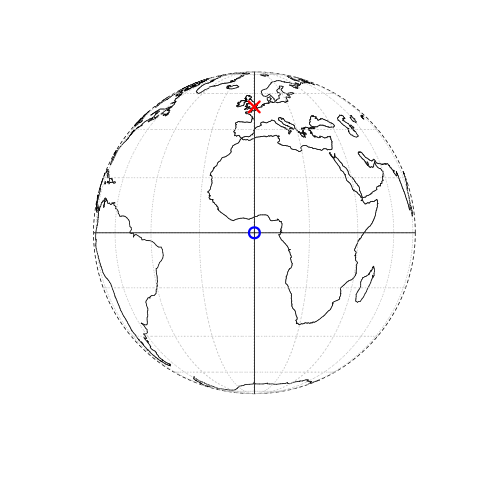
\includegraphics{images/vector_lonlat.png}\end{minipage}%
%
\begin{minipage}{0.50\linewidth}
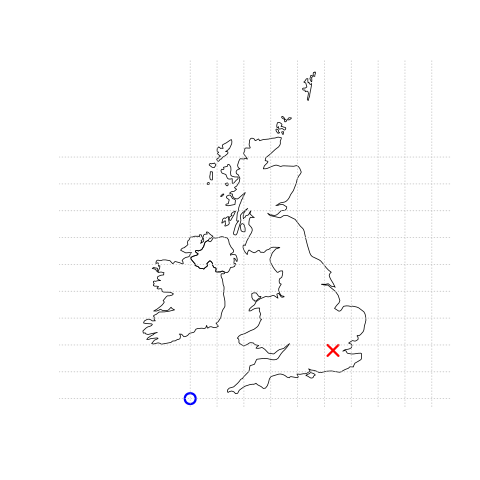
\includegraphics{images/vector_projected.png}\end{minipage}%

\caption{\label{fig-vector-london}Illustration of vector (point) data in
which location of London (the red X) is represented with reference to an
origin (the blue circle). The left plot represents a geographic CRS with
an origin at 0° longitude and latitude. The right plot represents a
projected CRS with an origin located in the sea west of the South West
Peninsula.}

\end{figure}%

There is more to CRSs, as described in
Section~\ref{sec-coordinate-reference-systems-intro} and
Chapter~\ref{sec-reproj-geo-data} but, for the purposes of this section,
it is sufficient to know that coordinates consist of two numbers
representing the distance from an origin, usually in \(x\) and \(y\)
dimensions.

\textbf{geopandas} (Bossche et al. 2023) provides classes for geographic
vector data and a consistent command-line interface for reproducible
geographic data analysis in Python. It also provides an interface to
three mature libraries for geocomputation, a strong foundation on which
many geographic applications are built:

\begin{itemize}
\tightlist
\item
  GDAL, for reading, writing, and manipulating a wide range of
  geographic data formats, covered in Chapter~\ref{sec-read-write}
\item
  PROJ, a powerful library for coordinate system transformations, which
  underlies the content covered in Chapter~\ref{sec-reproj-geo-data}
\item
  GEOS, a planar geometry engine for operations such as calculating
  buffers and centroids on data with a projected CRS, covered in
  Chapter~\ref{sec-geometric-operations}
\end{itemize}

Tight integration with these geographic libraries makes reproducible
geocomputation possible: an advantage of using a higher-level language
such as Python to access these libraries is that you do not need to know
the intricacies of the low-level components, enabling focus on the
methods rather than the implementation.

\subsection{Vector data classes}\label{vector-data-classes}

The main classes for working with geographic vector data in Python are
hierarchical, meaning that the `vector layer' class is composed of
simpler `geometry column' and individual `geometry' components. This
section introduces them in order, starting with the highest level class.
For many applications, the vector layer class, a data frame with
geometry columns, is all that's needed. However, it's important to
understand the structure of vector geographic objects and their
components for some applications and for a deep understanding. The three
main vector geographic data classes in Python are:

\begin{itemize}
\tightlist
\item
  \texttt{GeoDataFrame}, a class representing vector layers, with a
  geometry column (class \texttt{GeoSeries}) as one of the columns
\item
  \texttt{GeoSeries}, a class that is used to represent the geometry
  column in \texttt{GeoDataFrame} objects
\item
  \texttt{shapely} geometry objects, which represent individual
  geometries, such as a point or a polygon in \texttt{GeoSeries} objects
\end{itemize}

The first two classes (\texttt{GeoDataFrame} and \texttt{GeoSeries}) are
defined in \textbf{geopandas}. The third class is defined in the
\textbf{shapely} package, which deals with individual geometries, and is
a main dependency of the \textbf{geopandas} package.

\subsection{Vector layers}\label{sec-vector-layers}

The most commonly used geographic vector data structure is the vector
layer. There are several approaches for working with vector layers in
Python, ranging from low-level packages (e.g., \textbf{osgeo},
\textbf{fiona}) to the relatively high-level \textbf{geopandas} package
that is the focus of this section. Before writing and running code for
creating and working with geographic vector objects, we need to import
\textbf{geopandas} (by convention as \texttt{gpd} for more concise code)
and \textbf{shapely}.

\begin{Shaded}
\begin{Highlighting}[]
\ImportTok{import}\NormalTok{ pandas }\ImportTok{as}\NormalTok{ pd}
\ImportTok{import}\NormalTok{ shapely}
\ImportTok{import}\NormalTok{ geopandas }\ImportTok{as}\NormalTok{ gpd}
\end{Highlighting}
\end{Shaded}

We also limit the maximum number of printed rows to six, to save space,
using the \texttt{\textquotesingle{}display.max\_rows\textquotesingle{}}
option of \textbf{pandas}.

\begin{Shaded}
\begin{Highlighting}[]
\NormalTok{pd.set\_option(}\StringTok{\textquotesingle{}display.max\_rows\textquotesingle{}}\NormalTok{, }\DecValTok{6}\NormalTok{)}
\end{Highlighting}
\end{Shaded}

Projects often start by importing an existing vector layer saved as a
GeoPackage (\texttt{.gpkg}) file, an ESRI Shapefile (\texttt{.shp}), or
other geographic file format. The function \texttt{gpd.read\_file}
imports a GeoPackage file named \texttt{world.gpkg} located in the
\texttt{data} directory of Python's working directory into a
\texttt{GeoDataFrame} named \texttt{gdf}.

\begin{Shaded}
\begin{Highlighting}[]
\NormalTok{gdf }\OperatorTok{=}\NormalTok{ gpd.read\_file(}\StringTok{\textquotesingle{}data/world.gpkg\textquotesingle{}}\NormalTok{)}
\end{Highlighting}
\end{Shaded}

The result is an object of type (class) \texttt{GeoDataFrame} with 177
rows (features) and 11 columns, as shown in the output of the following
code:

\begin{Shaded}
\begin{Highlighting}[]
\BuiltInTok{type}\NormalTok{(gdf)}
\end{Highlighting}
\end{Shaded}

\phantomsection\label{typegdf}
\begin{verbatim}
geopandas.geodataframe.GeoDataFrame
\end{verbatim}

\begin{Shaded}
\begin{Highlighting}[]
\NormalTok{gdf.shape}
\end{Highlighting}
\end{Shaded}

\begin{verbatim}
(177, 11)
\end{verbatim}

The \texttt{GeoDataFrame} class is an extension of the
\texttt{DataFrame} class from the popular \textbf{pandas} package
(McKinney 2010). This means we can treat non-spatial attributes from a
vector layer as a table, and process them using the ordinary, i.e.,
non-spatial, established function methods. For example, standard data
frame subsetting methods can be used. The code below creates a subset of
the \texttt{gdf} dataset containing only the country name and the
geometry.

\begin{Shaded}
\begin{Highlighting}[]
\NormalTok{gdf }\OperatorTok{=}\NormalTok{ gdf[[}\StringTok{\textquotesingle{}name\_long\textquotesingle{}}\NormalTok{, }\StringTok{\textquotesingle{}geometry\textquotesingle{}}\NormalTok{]]}
\NormalTok{gdf}
\end{Highlighting}
\end{Shaded}

\begin{longtable}[]{@{}lll@{}}
\toprule\noalign{}
& name\_long & geometry \\
\midrule\noalign{}
\endhead
\bottomrule\noalign{}
\endlastfoot
0 & Fiji & MULTIPOLYGON (((-180 -16.55522,... \\
1 & Tanzania & MULTIPOLYGON (((33.90371 -0.95,... \\
2 & Western Sahara & MULTIPOLYGON (((-8.66559 27.656... \\
... & ... & ... \\
174 & Kosovo & MULTIPOLYGON (((20.59025 41.855... \\
175 & Trinidad and Tobago & MULTIPOLYGON (((-61.68 10.76, -... \\
176 & South Sudan & MULTIPOLYGON (((30.83385 3.5091... \\
\end{longtable}

The following expression creates a subdataset based on a condition, such
as equality of the value in the
\texttt{\textquotesingle{}name\_long\textquotesingle{}} column to the
string \texttt{\textquotesingle{}Egypt\textquotesingle{}}.

\begin{Shaded}
\begin{Highlighting}[]
\NormalTok{gdf[gdf[}\StringTok{\textquotesingle{}name\_long\textquotesingle{}}\NormalTok{] }\OperatorTok{==} \StringTok{\textquotesingle{}Egypt\textquotesingle{}}\NormalTok{]}
\end{Highlighting}
\end{Shaded}

\begin{longtable}[]{@{}lll@{}}
\toprule\noalign{}
& name\_long & geometry \\
\midrule\noalign{}
\endhead
\bottomrule\noalign{}
\endlastfoot
163 & Egypt & MULTIPOLYGON (((36.86623 22, 36... \\
\end{longtable}

Finally, to get a sense of the spatial component of the vector layer, it
can be plotted using the \texttt{.plot} method
(Figure~\ref{fig-gdf-plot}).

\begin{Shaded}
\begin{Highlighting}[]
\NormalTok{gdf.plot()}\OperatorTok{;}
\end{Highlighting}
\end{Shaded}

\begin{figure}[H]

\centering{

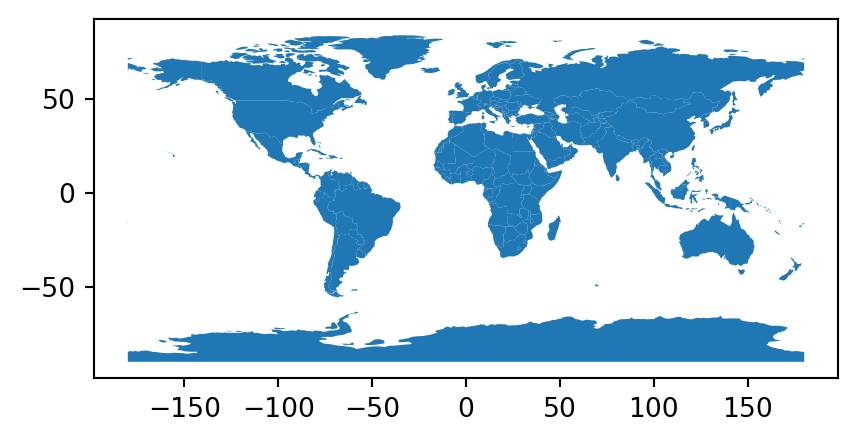
\includegraphics{01-spatial-data_files/figure-pdf/fig-gdf-plot-output-1.pdf}

}

\caption{\label{fig-gdf-plot}Basic plot of a \texttt{GeoDataFrame}}

\end{figure}%

Interactive maps of \texttt{GeoDataFrame} objects can be created with
the \texttt{.explore} method, as illustrated in
Figure~\ref{fig-gdf-explore} which was created with the following
command:

\begin{Shaded}
\begin{Highlighting}[]
\NormalTok{gdf.explore()}
\end{Highlighting}
\end{Shaded}

\begin{figure}

\centering{

\includegraphics{images/fig-gdf-explore.png}

}

\caption{\label{fig-gdf-explore}Basic interactive map with
\texttt{.explore}}

\end{figure}%

A subset of the data can be also plotted in a similar fashion.

\begin{Shaded}
\begin{Highlighting}[]
\NormalTok{gdf[gdf[}\StringTok{\textquotesingle{}name\_long\textquotesingle{}}\NormalTok{] }\OperatorTok{==} \StringTok{\textquotesingle{}Egypt\textquotesingle{}}\NormalTok{].explore()}
\end{Highlighting}
\end{Shaded}

\begin{figure}

\centering{

\includegraphics{images/fig-gdf-explore2.png}

}

\caption{\label{fig-gdf-explore2}Interactive map of a
\texttt{GeoDataFrame} subset}

\end{figure}%

\subsection{Geometry columns}\label{sec-geometry-columns}

The geometry column of class \texttt{GeoSeries} is an essential column
in a \texttt{GeoDataFrame}. It contains the geometric part of the vector
layer, and is the basis for all spatial operations. This column can be
accessed by name, which typically (e.g., when reading from a file) is
\texttt{\textquotesingle{}geometry\textquotesingle{}}, as in
\texttt{gdf{[}\textquotesingle{}geometry\textquotesingle{}{]}}. However,
the recommendation is to use the fixed \texttt{.geometry} property,
which refers to the geometry column regardless whether its name is
\texttt{\textquotesingle{}geometry\textquotesingle{}} or not. In the
case of the \texttt{gdf} object, the geometry column contains
\texttt{\textquotesingle{}MultiPolygon\textquotesingle{}}s associated
with each country.

\begin{Shaded}
\begin{Highlighting}[]
\NormalTok{gdf.geometry}
\end{Highlighting}
\end{Shaded}

\begin{verbatim}
0      MULTIPOLYGON (((-180 -16.55522,...
1      MULTIPOLYGON (((33.90371 -0.95,...
2      MULTIPOLYGON (((-8.66559 27.656...
                      ...                
174    MULTIPOLYGON (((20.59025 41.855...
175    MULTIPOLYGON (((-61.68 10.76, -...
176    MULTIPOLYGON (((30.83385 3.5091...
Name: geometry, Length: 177, dtype: geometry
\end{verbatim}

The geometry column also contains the spatial reference information, if
any (also accessible with the shortcut \texttt{gdf.crs}).

\begin{Shaded}
\begin{Highlighting}[]
\NormalTok{gdf.geometry.crs}
\end{Highlighting}
\end{Shaded}

\begin{verbatim}
<Geographic 2D CRS: EPSG:4326>
Name: WGS 84
Axis Info [ellipsoidal]:
- Lat[north]: Geodetic latitude (degree)
- Lon[east]: Geodetic longitude (degree)
Area of Use:
- name: World.
- bounds: (-180.0, -90.0, 180.0, 90.0)
Datum: World Geodetic System 1984 ensemble
- Ellipsoid: WGS 84
- Prime Meridian: Greenwich
\end{verbatim}

Many geometry operations, such as calculating the centroid, buffer, or
bounding box of each feature, involve just the geometry. Applying this
type of operation on a \texttt{GeoDataFrame} is therefore basically a
shortcut to applying it on the \texttt{GeoSeries} object in the geometry
column. For example, the two following commands return exactly the same
result, a \texttt{GeoSeries} containing bounding box polygons (using the
\texttt{.envelope} method).

\begin{Shaded}
\begin{Highlighting}[]
\NormalTok{gdf.envelope}
\end{Highlighting}
\end{Shaded}

\begin{verbatim}
0      POLYGON ((-180 -18.28799, 179.9...
1      POLYGON ((29.34 -11.72094, 40.3...
2      POLYGON ((-17.06342 20.99975, -...
                      ...                
174    POLYGON ((20.0707 41.84711, 21....
175    POLYGON ((-61.95 10, -60.895 10...
176    POLYGON ((23.88698 3.50917, 35....
Length: 177, dtype: geometry
\end{verbatim}

\begin{Shaded}
\begin{Highlighting}[]
\NormalTok{gdf.geometry.envelope}
\end{Highlighting}
\end{Shaded}

\begin{verbatim}
0      POLYGON ((-180 -18.28799, 179.9...
1      POLYGON ((29.34 -11.72094, 40.3...
2      POLYGON ((-17.06342 20.99975, -...
                      ...                
174    POLYGON ((20.0707 41.84711, 21....
175    POLYGON ((-61.95 10, -60.895 10...
176    POLYGON ((23.88698 3.50917, 35....
Length: 177, dtype: geometry
\end{verbatim}

Note that \texttt{.envelope}, and other similar operators in
\textbf{geopandas} such as \texttt{.centroid}
(Section~\ref{sec-centroids}), \texttt{.buffer}
(Section~\ref{sec-buffers}), or \texttt{.convex\_hull}, return only the
geometry (i.e., a \texttt{GeoSeries}), not a \texttt{GeoDataFrame} with
the original attribute data. In case we want the latter, we can create a
copy of the \texttt{GeoDataFrame} and then `overwrite' its geometry (or,
we can overwrite the geometries directly in case we do not need the
original ones, as in \texttt{gdf.geometry=gdf.envelope}).

\begin{Shaded}
\begin{Highlighting}[]
\NormalTok{gdf2 }\OperatorTok{=}\NormalTok{ gdf.copy()}
\NormalTok{gdf2.geometry }\OperatorTok{=}\NormalTok{ gdf.envelope}
\NormalTok{gdf2}
\end{Highlighting}
\end{Shaded}

\begin{longtable}[]{@{}lll@{}}
\toprule\noalign{}
& name\_long & geometry \\
\midrule\noalign{}
\endhead
\bottomrule\noalign{}
\endlastfoot
0 & Fiji & POLYGON ((-180 -18.28799, 179.9... \\
1 & Tanzania & POLYGON ((29.34 -11.72094, 40.3... \\
2 & Western Sahara & POLYGON ((-17.06342 20.99975, -... \\
... & ... & ... \\
174 & Kosovo & POLYGON ((20.0707 41.84711, 21.... \\
175 & Trinidad and Tobago & POLYGON ((-61.95 10, -60.895 10... \\
176 & South Sudan & POLYGON ((23.88698 3.50917, 35.... \\
\end{longtable}

Another useful property of the geometry column is the geometry type, as
shown in the following code. Note that the types of geometries contained
in a geometry column (and, thus, a vector layer) are not necessarily the
same for every row. It is possible to have multiple geometry types in a
single \texttt{GeoSeries}. Accordingly, the \texttt{.type} property
returns a \texttt{Series} (with values of type \texttt{str}, i.e.,
strings), rather than a single value (the same can be done with the
shortcut \texttt{gdf.geom\_type}).

\begin{Shaded}
\begin{Highlighting}[]
\NormalTok{gdf.geometry.}\BuiltInTok{type}
\end{Highlighting}
\end{Shaded}

\begin{verbatim}
0      MultiPolygon
1      MultiPolygon
2      MultiPolygon
           ...     
174    MultiPolygon
175    MultiPolygon
176    MultiPolygon
Length: 177, dtype: object
\end{verbatim}

To summarize the occurrence of different geometry types in a geometry
column, we can use the \textbf{pandas} \texttt{.value\_counts} method.
In this case, we see that the \texttt{gdf} layer contains only
\texttt{\textquotesingle{}MultiPolygon\textquotesingle{}} geometries.

\begin{Shaded}
\begin{Highlighting}[]
\NormalTok{gdf.geometry.}\BuiltInTok{type}\NormalTok{.value\_counts()}
\end{Highlighting}
\end{Shaded}

\begin{verbatim}
MultiPolygon    177
Name: count, dtype: int64
\end{verbatim}

A \texttt{GeoDataFrame} can also have multiple \texttt{GeoSeries}
columns, as demonstrated in the following code section.

\begin{Shaded}
\begin{Highlighting}[]
\NormalTok{gdf[}\StringTok{\textquotesingle{}bbox\textquotesingle{}}\NormalTok{] }\OperatorTok{=}\NormalTok{ gdf.envelope}
\NormalTok{gdf[}\StringTok{\textquotesingle{}polygon\textquotesingle{}}\NormalTok{] }\OperatorTok{=}\NormalTok{ gdf.geometry}
\NormalTok{gdf}
\end{Highlighting}
\end{Shaded}

Only one geometry column at a time is `active', in the sense that it is
being accessed in operations involving the geometries (such as
\texttt{.centroid}, \texttt{.crs}, etc.). To switch the active geometry
column from one \texttt{GeoSeries} column to another, we use
\texttt{.set\_geometry}. Figure~\ref{fig-switch-to-centroids} and
Figure~\ref{fig-switch-to-polygons} shows interactive maps of the
\texttt{gdf} layer with the
\texttt{\textquotesingle{}bbox\textquotesingle{}} and
\texttt{\textquotesingle{}polygon\textquotesingle{}} geometry columns
activated, respectively.

\begin{Shaded}
\begin{Highlighting}[]
\NormalTok{gdf }\OperatorTok{=}\NormalTok{ gdf.set\_geometry(}\StringTok{\textquotesingle{}bbox\textquotesingle{}}\NormalTok{)}
\NormalTok{gdf.explore()}
\end{Highlighting}
\end{Shaded}

\begin{figure}

\centering{

\includegraphics{images/fig-switch-to-centroids.png}

}

\caption{\label{fig-switch-to-centroids}Switching to the
\texttt{\textquotesingle{}bbox\textquotesingle{}} geometry column in the
\texttt{world} layer, and plotting it}

\end{figure}%

\begin{Shaded}
\begin{Highlighting}[]
\NormalTok{gdf }\OperatorTok{=}\NormalTok{ gdf.set\_geometry(}\StringTok{\textquotesingle{}polygon\textquotesingle{}}\NormalTok{)}
\NormalTok{gdf.explore()}
\end{Highlighting}
\end{Shaded}

\begin{figure}

\centering{

\includegraphics{images/fig-switch-to-polygons.png}

}

\caption{\label{fig-switch-to-polygons}Switching to the
\texttt{\textquotesingle{}polygons\textquotesingle{}} geometry column in
the \texttt{world} layer, and plotting it}

\end{figure}%

\subsection{The Simple Features standard}\label{sec-simple-features}

Geometries are the basic building blocks of vector layers. Although the
Simple Features standard defines about 20 types of geometries, we will
focus on the seven most commonly used types: \texttt{POINT},
\texttt{LINESTRING}, \texttt{POLYGON}, \texttt{MULTIPOINT},
\texttt{MULTILINESTRING}, \texttt{MULTIPOLYGON} and
\texttt{GEOMETRYCOLLECTION}. A useful list of possible geometry types
can be found in R's \textbf{sf} package documentation\footnote{\url{https://r-spatial.github.io/sf/articles/sf1.html\#simple-feature-geometry-types}}.

Simple feature geometries can be represented by well-known binary (WKB)
and well-known text (WKT) encodings. WKB representations are usually
hexadecimal strings easily readable for computers, and this is why GIS
software and spatial databases use WKB to transfer and store geometry
objects. WKT, on the other hand, is a human-readable text markup
description of Simple Features. Both formats are exchangeable, and if we
present one, we will naturally choose the WKT representation.

The foundation of each geometry type is the point. A point is simply a
coordinate in two-dimensional, three-dimensional, or four-dimensional
space such as shown in Figure~\ref{fig-point}.

\begin{Shaded}
\begin{Highlighting}[]
\NormalTok{POINT (5 2)}
\end{Highlighting}
\end{Shaded}

A linestring is a sequence of points with a straight line connecting the
points (Figure~\ref{fig-linestring}).

\begin{Shaded}
\begin{Highlighting}[]
\NormalTok{LINESTRING (1 5, 4 4, 4 1, 2 2, 3 2)}
\end{Highlighting}
\end{Shaded}

A polygon is a sequence of points that form a closed, non-intersecting
ring. Closed means that the first and the last point of a polygon have
the same coordinates (Figure~\ref{fig-polygon}).

\begin{Shaded}
\begin{Highlighting}[]
\NormalTok{POLYGON ((1 5, 2 2, 4 1, 4 4, 1 5))}
\end{Highlighting}
\end{Shaded}

So far we have created geometries with only one geometric entity per
feature. However, the Simple Features standard allows multiple
geometries to exist within a single feature, using `multi' versions of
each geometry type, as illustrated in Figure~\ref{fig-multipoint},
Figure~\ref{fig-multilinestring}, and Figure~\ref{fig-multipolygon1}.

\begin{Shaded}
\begin{Highlighting}[]
\NormalTok{MULTIPOINT (5 2, 1 3, 3 4, 3 2)}
\NormalTok{MULTILINESTRING ((1 5, 4 4, 4 1, 2 2, 3 2), (1 2, 2 4))}
\NormalTok{MULTIPOLYGON (((1 5, 2 2, 4 1, 4 4, 1 5), (0 2, 1 2, 1 3, 0 3, 0 2)))}
\end{Highlighting}
\end{Shaded}

Finally, a geometry collection can contain any combination of geometries
of the other six types, such as the combination of a multipoint and
linestring shown below (Figure~\ref{fig-geometrycollection}).

\begin{Shaded}
\begin{Highlighting}[]
\NormalTok{GEOMETRYCOLLECTION (MULTIPOINT (5 2, 1 3, 3 4, 3 2),}
\NormalTok{                    LINESTRING (1 5, 4 4, 4 1, 2 2, 3 2))}
\end{Highlighting}
\end{Shaded}

\subsection{Geometries}\label{sec-geometries}

Each element in the geometry column (\texttt{GeoSeries}) is a geometry
object of class \texttt{shapely} (Gillies et al. 2007-\/-). For example,
here is one specific geometry selected by implicit index (Canada, the
4\textsuperscript{th} element in \texttt{gdf}'s geometry column).

\begin{Shaded}
\begin{Highlighting}[]
\NormalTok{gdf.geometry.iloc[}\DecValTok{3}\NormalTok{]}
\end{Highlighting}
\end{Shaded}


\includegraphics{index_files/mediabag/01-spatial-data_files/figure-pdf/cell-34-output-1.pdf}

We can also select a specific geometry based on the
\texttt{\textquotesingle{}name\_long\textquotesingle{}} attribute (i.e.,
the 1\textsuperscript{st} and only element in the subset of \texttt{gdf}
where the country name is equal to \texttt{Egypt}):

\begin{Shaded}
\begin{Highlighting}[]
\NormalTok{gdf[gdf[}\StringTok{\textquotesingle{}name\_long\textquotesingle{}}\NormalTok{] }\OperatorTok{==} \StringTok{\textquotesingle{}Egypt\textquotesingle{}}\NormalTok{].geometry.iloc[}\DecValTok{0}\NormalTok{]}
\end{Highlighting}
\end{Shaded}


\includegraphics{index_files/mediabag/01-spatial-data_files/figure-pdf/cell-35-output-1.pdf}

The \textbf{shapely} package is compatible with the Simple Features
standard (Section~\ref{sec-simple-features}). Accordingly, seven types
of geometry types are supported. The following section demonstrates
creating a \texttt{shapely} geometry of each type from scratch. In the
first example (a \texttt{\textquotesingle{}Point\textquotesingle{}}) we
show two types of inputs to create a geometry: a list of coordinates or
a \texttt{string} in the WKT format. In the examples for the remaining
geometries we use the former approach.

Creating a \texttt{\textquotesingle{}Point\textquotesingle{}} geometry
from a list of coordinates uses the \texttt{shapely.Point} function in
the following expression (Figure~\ref{fig-point}).

\begin{Shaded}
\begin{Highlighting}[]
\NormalTok{point }\OperatorTok{=}\NormalTok{ shapely.Point([}\DecValTok{5}\NormalTok{, }\DecValTok{2}\NormalTok{])}
\NormalTok{point}
\end{Highlighting}
\end{Shaded}

\begin{figure}[H]

\centering{

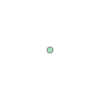
\includegraphics{index_files/mediabag/01-spatial-data_files/figure-pdf/fig-point-output-1.pdf}

}

\caption{\label{fig-point}A \texttt{Point} geometry (created either from
a \texttt{list} or WKT)}

\end{figure}%

Alternatively, we can use \texttt{shapely.from\_wkt} to transform a WKT
string to a \texttt{shapely} geometry object. Here is an example of
creating the same \texttt{\textquotesingle{}Point\textquotesingle{}}
geometry from WKT (Figure~\ref{fig-point}).

\begin{Shaded}
\begin{Highlighting}[]
\NormalTok{point }\OperatorTok{=}\NormalTok{ shapely.from\_wkt(}\StringTok{\textquotesingle{}POINT (5 2)\textquotesingle{}}\NormalTok{)}
\NormalTok{point}
\end{Highlighting}
\end{Shaded}

A \texttt{\textquotesingle{}LineString\textquotesingle{}} geometry can
be created based on a list of coordinate tuples or lists
(Figure~\ref{fig-linestring}).

\begin{Shaded}
\begin{Highlighting}[]
\NormalTok{linestring }\OperatorTok{=}\NormalTok{ shapely.LineString([(}\DecValTok{1}\NormalTok{,}\DecValTok{5}\NormalTok{), (}\DecValTok{4}\NormalTok{,}\DecValTok{4}\NormalTok{), (}\DecValTok{4}\NormalTok{,}\DecValTok{1}\NormalTok{), (}\DecValTok{2}\NormalTok{,}\DecValTok{2}\NormalTok{), (}\DecValTok{3}\NormalTok{,}\DecValTok{2}\NormalTok{)])}
\NormalTok{linestring}
\end{Highlighting}
\end{Shaded}

\begin{figure}[H]

\centering{

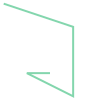
\includegraphics{index_files/mediabag/01-spatial-data_files/figure-pdf/fig-linestring-output-1.pdf}

}

\caption{\label{fig-linestring}A \texttt{LineString} geometry}

\end{figure}%

Creation of a \texttt{\textquotesingle{}Polygon\textquotesingle{}}
geometry is similar, but our first and last coordinate must be the same,
to ensure that the polygon is closed. Note that in the following
example, there is one list of coordinates that defines the exterior
outer hull of the polygon, followed by a \texttt{list} of \texttt{list}s
of coordinates that define the holes (if any) in the polygon
(Figure~\ref{fig-polygon}).

\begin{Shaded}
\begin{Highlighting}[]
\NormalTok{polygon }\OperatorTok{=}\NormalTok{ shapely.Polygon(}
\NormalTok{    [(}\DecValTok{1}\NormalTok{,}\DecValTok{5}\NormalTok{), (}\DecValTok{2}\NormalTok{,}\DecValTok{2}\NormalTok{), (}\DecValTok{4}\NormalTok{,}\DecValTok{1}\NormalTok{), (}\DecValTok{4}\NormalTok{,}\DecValTok{4}\NormalTok{), (}\DecValTok{1}\NormalTok{,}\DecValTok{5}\NormalTok{)],  }\CommentTok{\#\# Exterior}
\NormalTok{    [[(}\DecValTok{2}\NormalTok{,}\DecValTok{4}\NormalTok{), (}\DecValTok{3}\NormalTok{,}\DecValTok{4}\NormalTok{), (}\DecValTok{3}\NormalTok{,}\DecValTok{3}\NormalTok{), (}\DecValTok{2}\NormalTok{,}\DecValTok{3}\NormalTok{), (}\DecValTok{2}\NormalTok{,}\DecValTok{4}\NormalTok{)]]  }\CommentTok{\#\# Hole(s)}
\NormalTok{)}
\NormalTok{polygon}
\end{Highlighting}
\end{Shaded}

\begin{figure}[H]

\centering{


\includegraphics{index_files/mediabag/01-spatial-data_files/figure-pdf/fig-polygon-output-1.pdf}

}

\caption{\label{fig-polygon}A \texttt{Polygon} geometry}

\end{figure}%

A \texttt{\textquotesingle{}MultiPoint\textquotesingle{}} geometry is
also created from a list of coordinate tuples
(Figure~\ref{fig-multipoint}), where each element represents a single
point.

\begin{Shaded}
\begin{Highlighting}[]
\NormalTok{multipoint }\OperatorTok{=}\NormalTok{ shapely.MultiPoint([(}\DecValTok{5}\NormalTok{,}\DecValTok{2}\NormalTok{), (}\DecValTok{1}\NormalTok{,}\DecValTok{3}\NormalTok{), (}\DecValTok{3}\NormalTok{,}\DecValTok{4}\NormalTok{), (}\DecValTok{3}\NormalTok{,}\DecValTok{2}\NormalTok{)])}
\NormalTok{multipoint}
\end{Highlighting}
\end{Shaded}

\begin{figure}[H]

\centering{

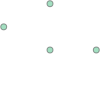
\includegraphics{index_files/mediabag/01-spatial-data_files/figure-pdf/fig-multipoint-output-1.pdf}

}

\caption{\label{fig-multipoint}A \texttt{MultiPoint} geometry}

\end{figure}%

A \texttt{\textquotesingle{}MultiLineString\textquotesingle{}} geometry,
on the other hand, has one list of coordinates for each line in the
\texttt{MultiLineString} (Figure~\ref{fig-multilinestring}).

\begin{Shaded}
\begin{Highlighting}[]
\NormalTok{multilinestring }\OperatorTok{=}\NormalTok{ shapely.MultiLineString([}
\NormalTok{    [(}\DecValTok{1}\NormalTok{,}\DecValTok{5}\NormalTok{), (}\DecValTok{4}\NormalTok{,}\DecValTok{4}\NormalTok{), (}\DecValTok{4}\NormalTok{,}\DecValTok{1}\NormalTok{), (}\DecValTok{2}\NormalTok{,}\DecValTok{2}\NormalTok{), (}\DecValTok{3}\NormalTok{,}\DecValTok{2}\NormalTok{)],  }\CommentTok{\#\# 1st sequence}
\NormalTok{    [(}\DecValTok{1}\NormalTok{,}\DecValTok{2}\NormalTok{), (}\DecValTok{2}\NormalTok{,}\DecValTok{4}\NormalTok{)]  }\CommentTok{\#\# 2nd sequence, etc.}
\NormalTok{])}
\NormalTok{multilinestring}
\end{Highlighting}
\end{Shaded}

\begin{figure}[H]

\centering{

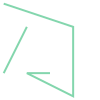
\includegraphics{index_files/mediabag/01-spatial-data_files/figure-pdf/fig-multilinestring-output-1.pdf}

}

\caption{\label{fig-multilinestring}A \texttt{MultiLineString} geometry}

\end{figure}%

A \texttt{\textquotesingle{}MultiPolygon\textquotesingle{}} geometry
(Figure~\ref{fig-multipolygon1}) is created from a \texttt{list} of
\texttt{Polygon} geometries. For example, here we are creating a
\texttt{\textquotesingle{}MultiPolygon\textquotesingle{}} with two
parts, both without holes.

\begin{Shaded}
\begin{Highlighting}[]
\NormalTok{multipolygon }\OperatorTok{=}\NormalTok{ shapely.MultiPolygon([}
\NormalTok{    [[(}\DecValTok{1}\NormalTok{,}\DecValTok{5}\NormalTok{), (}\DecValTok{2}\NormalTok{,}\DecValTok{2}\NormalTok{), (}\DecValTok{4}\NormalTok{,}\DecValTok{1}\NormalTok{), (}\DecValTok{4}\NormalTok{,}\DecValTok{4}\NormalTok{), (}\DecValTok{1}\NormalTok{,}\DecValTok{5}\NormalTok{)], []],  }\CommentTok{\#\# Polygon 1 }
\NormalTok{    [[(}\DecValTok{0}\NormalTok{,}\DecValTok{2}\NormalTok{), (}\DecValTok{1}\NormalTok{,}\DecValTok{2}\NormalTok{), (}\DecValTok{1}\NormalTok{,}\DecValTok{3}\NormalTok{), (}\DecValTok{0}\NormalTok{,}\DecValTok{3}\NormalTok{), (}\DecValTok{0}\NormalTok{,}\DecValTok{2}\NormalTok{)], []]   }\CommentTok{\#\# Polygon 2, etc.}
\NormalTok{])}
\NormalTok{multipolygon}
\end{Highlighting}
\end{Shaded}

\begin{figure}[H]

\centering{


\includegraphics{index_files/mediabag/01-spatial-data_files/figure-pdf/fig-multipolygon1-output-1.pdf}

}

\caption{\label{fig-multipolygon1}A \texttt{MultiPolygon} geometry}

\end{figure}%

Since the required input has four hierarchical levels, it may be more
clear to create the single-part
\texttt{\textquotesingle{}Polygon\textquotesingle{}} geometries in
advance, using the respective function (\texttt{shapely.Polygon}), and
then pass them to \texttt{shapely.MultiPolygon}
(Figure~\ref{fig-multipolygon1}). (The same technique can be used with
the other \texttt{shapely.Multi*} functions.)

\begin{Shaded}
\begin{Highlighting}[]
\NormalTok{multipolygon }\OperatorTok{=}\NormalTok{ shapely.MultiPolygon([}
\NormalTok{    shapely.Polygon([(}\DecValTok{1}\NormalTok{,}\DecValTok{5}\NormalTok{), (}\DecValTok{2}\NormalTok{,}\DecValTok{2}\NormalTok{), (}\DecValTok{4}\NormalTok{,}\DecValTok{1}\NormalTok{), (}\DecValTok{4}\NormalTok{,}\DecValTok{4}\NormalTok{), (}\DecValTok{1}\NormalTok{,}\DecValTok{5}\NormalTok{)]),  }\CommentTok{\#\# Polygon 1 }
\NormalTok{    shapely.Polygon([(}\DecValTok{0}\NormalTok{,}\DecValTok{2}\NormalTok{), (}\DecValTok{1}\NormalTok{,}\DecValTok{2}\NormalTok{), (}\DecValTok{1}\NormalTok{,}\DecValTok{3}\NormalTok{), (}\DecValTok{0}\NormalTok{,}\DecValTok{3}\NormalTok{), (}\DecValTok{0}\NormalTok{,}\DecValTok{2}\NormalTok{)])   }\CommentTok{\#\# Polygon 2, etc.}
\NormalTok{])}
\NormalTok{multipolygon}
\end{Highlighting}
\end{Shaded}

And, finally, a
\texttt{\textquotesingle{}GeometryCollection\textquotesingle{}} geometry
is a \texttt{list} with one or more of the other six geometry types
(Figure~\ref{fig-geometrycollection}):

\begin{Shaded}
\begin{Highlighting}[]
\NormalTok{geometrycollection }\OperatorTok{=}\NormalTok{ shapely.GeometryCollection([multipoint, multilinestring])}
\NormalTok{geometrycollection}
\end{Highlighting}
\end{Shaded}

\begin{figure}[H]

\centering{

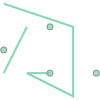
\includegraphics{index_files/mediabag/01-spatial-data_files/figure-pdf/fig-geometrycollection-output-1.pdf}

}

\caption{\label{fig-geometrycollection}A \texttt{GeometryCollection}
geometry}

\end{figure}%

\texttt{shapely} geometries act as atomic units of vector data, meaning
that there is no concept of geometry \emph{sets}: each operation accepts
individual geometry object(s) as input, and returns an individual
geometry as output. (The \texttt{GeoSeries} and \texttt{GeoDataFrame}
objects, defined in \textbf{geopandas}, are used to deal with sets of
\texttt{shapely} geometries, collectively.) For example, the following
expression calculates the difference (see Section~\ref{sec-clipping})
between the buffered (see Section~\ref{sec-buffers})
\texttt{multipolygon} (using distance of \texttt{0.2}) and itself
(Figure~\ref{fig-mpol-buffer-difference}):

\begin{Shaded}
\begin{Highlighting}[]
\NormalTok{multipolygon.}\BuiltInTok{buffer}\NormalTok{(}\FloatTok{0.2}\NormalTok{).difference(multipolygon)}
\end{Highlighting}
\end{Shaded}

\begin{figure}[H]

\centering{


\includegraphics{index_files/mediabag/01-spatial-data_files/figure-pdf/fig-mpol-buffer-difference-output-1.pdf}

}

\caption{\label{fig-mpol-buffer-difference}The difference between a
buffered \texttt{MultiPolygon} and itself}

\end{figure}%

As demonstrated in the last few figures, a \texttt{shapely} geometry
object is automatically evaluated to a small image of the geometry (when
using an interface capable of displaying it, such as Jupyter Notebook).
To print the WKT string instead, we can use the \texttt{print} function:

\begin{Shaded}
\begin{Highlighting}[]
\BuiltInTok{print}\NormalTok{(linestring)}
\end{Highlighting}
\end{Shaded}

\begin{verbatim}
LINESTRING (1 5, 4 4, 4 1, 2 2, 3 2)
\end{verbatim}

Finally, it is important to note that raw coordinates of
\texttt{shapely} geometries are accessible through a combination of the
\texttt{.coords}, \texttt{.geoms}, \texttt{.exterior}, and
\texttt{.interiors} properties (depending on the geometry type). These
access methods are helpful when we need to develop our own spatial
operators for specific tasks. For example, the following expression
returns the \texttt{list} of all coordinates of the \texttt{polygon}
geometry exterior:

\begin{Shaded}
\begin{Highlighting}[]
\BuiltInTok{list}\NormalTok{(polygon.exterior.coords)}
\end{Highlighting}
\end{Shaded}

\begin{verbatim}
[(1.0, 5.0), (2.0, 2.0), (4.0, 1.0), (4.0, 4.0), (1.0, 5.0)]
\end{verbatim}

Also see Section~\ref{sec-type-transformations}, where \texttt{.coords},
\texttt{.geoms}, and \texttt{.exterior} are used to transform a given
\texttt{shapely} geometry to a different type (e.g.,
\texttt{\textquotesingle{}Polygon\textquotesingle{}} to
\texttt{\textquotesingle{}MultiPoint\textquotesingle{}}).

\subsection{Vector layer from
scratch}\label{sec-vector-layer-from-scratch}

In the previous sections, we started with a vector layer
(\texttt{GeoDataFrame}), from an existing GeoPackage file, and
`decomposed' it to extract the geometry column (\texttt{GeoSeries},
Section~\ref{sec-geometry-columns}) and separate geometries
(\texttt{shapely}, see Section~\ref{sec-geometries}). In this section,
we will demonstrate the opposite process, constructing a
\texttt{GeoDataFrame} from \texttt{shapely} geometries, combined into a
\texttt{GeoSeries}. This will help you better understand the structure
of a \texttt{GeoDataFrame}, and may come in handy when you need to
programmatically construct simple vector layers, such as a line between
two given points.

Vector layers consist of two main parts: geometries and non-geographic
attributes. Figure~\ref{fig-gdf-flow} shows how a \texttt{GeoDataFrame}
object is created---geometries come from a \texttt{GeoSeries} object
(which consists of \texttt{shapely} geometries), while attributes are
taken from \texttt{Series} objects.

\begin{figure}

\centering{

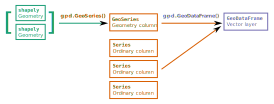
\includegraphics{index_files/mediabag/images/gdf-flow.pdf}

}

\caption{\label{fig-gdf-flow}Creating a \texttt{GeoDataFrame} from
scratch}

\end{figure}%

The final result, a vector layer (\texttt{GeoDataFrame}) is therefore a
hierarchical structure (Figure~\ref{fig-gdf-structure}), containing the
geometry column (\texttt{GeoSeries}), which in turn contains geometries
(\texttt{shapely}). Each of the `internal' components can be accessed,
or `extracted', which is sometimes necessary, as we will see later on.

\begin{figure}

\centering{

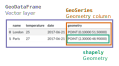
\includegraphics[width=0.5\textwidth,height=\textheight]{index_files/mediabag/images/gdf-structure.pdf}

}

\caption{\label{fig-gdf-structure}Structure of a \texttt{GeoDataFrame}}

\end{figure}%

Non-geographic attributes may represent the name of the feature, and
other attributes such as measured values, groups, etc. To illustrate
attributes, we will represent a temperature of 25°C in London on June
21st, 2023. This example contains a geometry (the coordinates), and
three attributes with three different classes (place name, temperature,
and date). Objects of class \texttt{GeoDataFrame} represent such data by
combining the attributes (\texttt{Series}) with the simple feature
geometry column (\texttt{GeoSeries}). First, we create a point geometry,
which we know how to do from Section~\ref{sec-geometries}
(Figure~\ref{fig-point-lnd}).

\begin{Shaded}
\begin{Highlighting}[]
\NormalTok{lnd\_point }\OperatorTok{=}\NormalTok{ shapely.Point(}\FloatTok{0.1}\NormalTok{, }\FloatTok{51.5}\NormalTok{)}
\NormalTok{lnd\_point}
\end{Highlighting}
\end{Shaded}

\begin{figure}[H]

\centering{

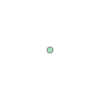
\includegraphics{index_files/mediabag/01-spatial-data_files/figure-pdf/fig-point-lnd-output-1.pdf}

}

\caption{\label{fig-point-lnd}A \texttt{shapely} point representing
London}

\end{figure}%

Next, we create a \texttt{GeoSeries} (of length 1), containing the point
and a CRS definition, in this case WGS84 (defined using its EPSG code
\texttt{4326}). Also note that the \texttt{shapely} geometries go into a
\texttt{list}, to illustrate that there can be more than one geometry
unlike in this example.

\begin{Shaded}
\begin{Highlighting}[]
\NormalTok{lnd\_geom }\OperatorTok{=}\NormalTok{ gpd.GeoSeries([lnd\_point], crs}\OperatorTok{=}\DecValTok{4326}\NormalTok{)}
\NormalTok{lnd\_geom}
\end{Highlighting}
\end{Shaded}

\begin{verbatim}
0    POINT (0.1 51.5)
dtype: geometry
\end{verbatim}

Next, we combine the \texttt{GeoSeries} with other attributes into a
\texttt{dict}. The geometry column is a \texttt{GeoSeries}, named
\texttt{geometry}. The other attributes (if any) may be defined using
\texttt{list} or \texttt{Series} objects. Here, for simplicity, we use
the \texttt{list} option for defining the three attributes
\texttt{name}, \texttt{temperature}, and \texttt{date}. Again, note that
the \texttt{list} can be of length \textgreater1, in case we are
creating a layer with more than one feature (i.e., multiple rows).

\begin{Shaded}
\begin{Highlighting}[]
\NormalTok{lnd\_data }\OperatorTok{=}\NormalTok{ \{}
  \StringTok{\textquotesingle{}name\textquotesingle{}}\NormalTok{: [}\StringTok{\textquotesingle{}London\textquotesingle{}}\NormalTok{],}
  \StringTok{\textquotesingle{}temperature\textquotesingle{}}\NormalTok{: [}\DecValTok{25}\NormalTok{],}
  \StringTok{\textquotesingle{}date\textquotesingle{}}\NormalTok{: [}\StringTok{\textquotesingle{}2023{-}06{-}21\textquotesingle{}}\NormalTok{],}
  \StringTok{\textquotesingle{}geometry\textquotesingle{}}\NormalTok{: lnd\_geom}
\NormalTok{\}}
\end{Highlighting}
\end{Shaded}

Finally, the \texttt{dict} can be converted to a \texttt{GeoDataFrame}
object, as shown in the following code.

\begin{Shaded}
\begin{Highlighting}[]
\NormalTok{lnd\_layer }\OperatorTok{=}\NormalTok{ gpd.GeoDataFrame(lnd\_data)}
\NormalTok{lnd\_layer}
\end{Highlighting}
\end{Shaded}

\begin{longtable}[]{@{}lllll@{}}
\toprule\noalign{}
& name & temperature & date & geometry \\
\midrule\noalign{}
\endhead
\bottomrule\noalign{}
\endlastfoot
0 & London & 25 & 2023-06-21 & POINT (0.1 51.5) \\
\end{longtable}

What just happened? First, the coordinates were used to create the
simple feature geometry (\texttt{shapely}). Second, the geometry was
converted into a simple feature geometry column (\texttt{GeoSeries}),
with a CRS. Third, attributes were combined with \texttt{GeoSeries}.
This results in an \texttt{GeoDataFrame} object, named
\texttt{lnd\_layer}.

To illustrate how does creating a layer with more than one feature looks
like, here is an example where we create a layer with two points, London
and Paris.

\begin{Shaded}
\begin{Highlighting}[]
\NormalTok{lnd\_point }\OperatorTok{=}\NormalTok{ shapely.Point(}\FloatTok{0.1}\NormalTok{, }\FloatTok{51.5}\NormalTok{)}
\NormalTok{paris\_point }\OperatorTok{=}\NormalTok{ shapely.Point(}\FloatTok{2.3}\NormalTok{, }\FloatTok{48.9}\NormalTok{)}
\NormalTok{towns\_geom }\OperatorTok{=}\NormalTok{ gpd.GeoSeries([lnd\_point, paris\_point], crs}\OperatorTok{=}\DecValTok{4326}\NormalTok{)}
\NormalTok{towns\_data }\OperatorTok{=}\NormalTok{ \{}
  \StringTok{\textquotesingle{}name\textquotesingle{}}\NormalTok{: [}\StringTok{\textquotesingle{}London\textquotesingle{}}\NormalTok{, }\StringTok{\textquotesingle{}Paris\textquotesingle{}}\NormalTok{],}
  \StringTok{\textquotesingle{}temperature\textquotesingle{}}\NormalTok{: [}\DecValTok{25}\NormalTok{, }\DecValTok{27}\NormalTok{],}
  \StringTok{\textquotesingle{}date\textquotesingle{}}\NormalTok{: [}\StringTok{\textquotesingle{}2013{-}06{-}21\textquotesingle{}}\NormalTok{, }\StringTok{\textquotesingle{}2013{-}06{-}21\textquotesingle{}}\NormalTok{],}
  \StringTok{\textquotesingle{}geometry\textquotesingle{}}\NormalTok{: towns\_geom}
\NormalTok{\}}
\NormalTok{towns\_layer }\OperatorTok{=}\NormalTok{ gpd.GeoDataFrame(towns\_data)}
\NormalTok{towns\_layer}
\end{Highlighting}
\end{Shaded}

\begin{longtable}[]{@{}lllll@{}}
\toprule\noalign{}
& name & temperature & date & geometry \\
\midrule\noalign{}
\endhead
\bottomrule\noalign{}
\endlastfoot
0 & London & 25 & 2013-06-21 & POINT (0.1 51.5) \\
1 & Paris & 27 & 2013-06-21 & POINT (2.3 48.9) \\
\end{longtable}

Now, we are able to create an interactive map of the
\texttt{towns\_layer} object
(Figure~\ref{fig-layer-from-scratch-explore}). To make the points easier
to see, we are customizing a fill color and size (we elaborate on
\texttt{.explore} options in Section~\ref{sec-interactive-maps}).

\begin{Shaded}
\begin{Highlighting}[]
\NormalTok{towns\_layer.explore(color}\OperatorTok{=}\StringTok{\textquotesingle{}red\textquotesingle{}}\NormalTok{, marker\_kwds}\OperatorTok{=}\NormalTok{\{}\StringTok{\textquotesingle{}radius\textquotesingle{}}\NormalTok{: }\DecValTok{10}\NormalTok{\})}
\end{Highlighting}
\end{Shaded}

\begin{figure}

\centering{

\includegraphics{images/fig-layer-from-scratch-explore.png}

}

\caption{\label{fig-layer-from-scratch-explore}\texttt{towns\_layer},
created from scratch, visualized using \texttt{.explore}}

\end{figure}%

A spatial (point) layer can be also created from a \texttt{DataFrame}
object (package \textbf{pandas}) that contains columns with coordinates.
To demonstrate, we hereby first create a \texttt{GeoSeries} object from
the coordinates, and then combine it with the \texttt{DataFrame} to form
a \texttt{GeoDataFrame}.

\begin{Shaded}
\begin{Highlighting}[]
\NormalTok{towns\_table }\OperatorTok{=}\NormalTok{ pd.DataFrame(\{}
  \StringTok{\textquotesingle{}name\textquotesingle{}}\NormalTok{: [}\StringTok{\textquotesingle{}London\textquotesingle{}}\NormalTok{, }\StringTok{\textquotesingle{}Paris\textquotesingle{}}\NormalTok{],}
  \StringTok{\textquotesingle{}temperature\textquotesingle{}}\NormalTok{: [}\DecValTok{25}\NormalTok{, }\DecValTok{27}\NormalTok{],}
  \StringTok{\textquotesingle{}date\textquotesingle{}}\NormalTok{: [}\StringTok{\textquotesingle{}2017{-}06{-}21\textquotesingle{}}\NormalTok{, }\StringTok{\textquotesingle{}2017{-}06{-}21\textquotesingle{}}\NormalTok{],}
  \StringTok{\textquotesingle{}x\textquotesingle{}}\NormalTok{: [}\FloatTok{0.1}\NormalTok{, }\FloatTok{2.3}\NormalTok{],}
  \StringTok{\textquotesingle{}y\textquotesingle{}}\NormalTok{: [}\FloatTok{51.5}\NormalTok{, }\FloatTok{48.9}\NormalTok{]}
\NormalTok{\})}
\NormalTok{towns\_geom }\OperatorTok{=}\NormalTok{ gpd.points\_from\_xy(towns\_table[}\StringTok{\textquotesingle{}x\textquotesingle{}}\NormalTok{], towns\_table[}\StringTok{\textquotesingle{}y\textquotesingle{}}\NormalTok{])}
\NormalTok{towns\_layer }\OperatorTok{=}\NormalTok{ gpd.GeoDataFrame(towns\_table, geometry}\OperatorTok{=}\NormalTok{towns\_geom, crs}\OperatorTok{=}\DecValTok{4326}\NormalTok{)}
\end{Highlighting}
\end{Shaded}

The output gives the same result as previous \texttt{towns\_layer}. This
approach is particularly useful when we need to read data from a CSV
file, e.g., using \texttt{pd.read\_csv}, and want to turn the resulting
\texttt{DataFrame} into a \texttt{GeoDataFrame} (see another example in
Section~\ref{sec-spatial-joining}).

\subsection{Derived numeric properties}\label{sec-area-length}

Vector layers are characterized by two essential derived numeric
properties: \emph{length} (\texttt{.length})---applicable to lines, and
\emph{area} (\texttt{.area})---applicable to polygons. Area and length
can be calculated for any data structures discussed above, either a
\texttt{shapely} geometry, in which case the returned value is a number,
or for \texttt{GeoSeries} or \texttt{DataFrame}, in which case the
returned value is a numeric \texttt{Series}.

\begin{Shaded}
\begin{Highlighting}[]
\NormalTok{linestring.length}
\end{Highlighting}
\end{Shaded}

\begin{verbatim}
9.39834563766817
\end{verbatim}

\begin{Shaded}
\begin{Highlighting}[]
\NormalTok{multipolygon.area}
\end{Highlighting}
\end{Shaded}

\begin{verbatim}
8.0
\end{verbatim}

\begin{Shaded}
\begin{Highlighting}[]
\NormalTok{gpd.GeoSeries([point, linestring, polygon, multipolygon]).area}
\end{Highlighting}
\end{Shaded}

\begin{verbatim}
0    0.0
1    0.0
2    6.0
3    8.0
dtype: float64
\end{verbatim}

Like all numeric calculations in \textbf{geopandas}, the results assume
a planar CRS and are returned in its native units. This means that
length and area measurements for geometries in WGS84 (\texttt{crs=4326})
are returned in decimal degrees and essentially meaningless (to see the
warning, try running \texttt{gdf.area}).

To obtain meaningful length and area measurements for data in a
geographic CRS, the geometries first need to be transformed to a
projected CRS (see Section~\ref{sec-reprojecting-vector-geometries})
applicable to the area of interest. For example, the area of Slovenia
can be calculated in the UTM zone 33N CRS (\texttt{crs=32633}). The
result is in \(m^2\), the units of the UTM zone 33N CRS.

\begin{Shaded}
\begin{Highlighting}[]
\NormalTok{gdf[gdf[}\StringTok{\textquotesingle{}name\_long\textquotesingle{}}\NormalTok{] }\OperatorTok{==} \StringTok{\textquotesingle{}Slovenia\textquotesingle{}}\NormalTok{].to\_crs(}\DecValTok{32633}\NormalTok{).area}
\end{Highlighting}
\end{Shaded}

\begin{verbatim}
150    1.910410e+10
dtype: float64
\end{verbatim}

\section{Raster data}\label{sec-raster-data}

The spatial raster data model represents the world with the continuous
grid of cells (often also called pixels;
Figure~\ref{fig-raster-intro-plot1} (A)). This data model often refers
to so-called regular grids, in which each cell has the same, constant
size---and we will focus only on regular grids in this book. However,
several other types of grids exist, including rotated, sheared,
rectilinear, and curvilinear grids (see Chapter 1 of Pebesma and Bivand
(2022) or Chapter 2 of Tennekes and Nowosad (2022)).

The raster data model usually consists of a raster header (or metadata)
and a matrix (with rows and columns) representing equally spaced cells
(often also called pixels; Figure~\ref{fig-raster-intro-plot1} (A)). The
raster header defines the coordinate reference system, the origin and
the resolution. The origin (or starting point) is typically the
coordinate of the lower-left corner of the matrix. The metadata defines
the origin, and the cell size, i.e., resolution. Combined with the
column and row count, the extent can also be derived. The matrix
representation avoids storing explicitly the coordinates for the four
corner points (in fact it only stores one coordinate, namely the origin)
of each cell, as would be the case for rectangular vector polygons. This
and map algebra (Section~\ref{sec-map-algebra}) makes raster processing
much more efficient and faster than vector data processing. However, in
contrast to vector data, the cell of one raster layer can only hold a
single value. The cell values are numeric, representing either a
continuous or a categorical variable
(Figure~\ref{fig-raster-intro-plot1} (C)).

\begin{figure}

\centering{

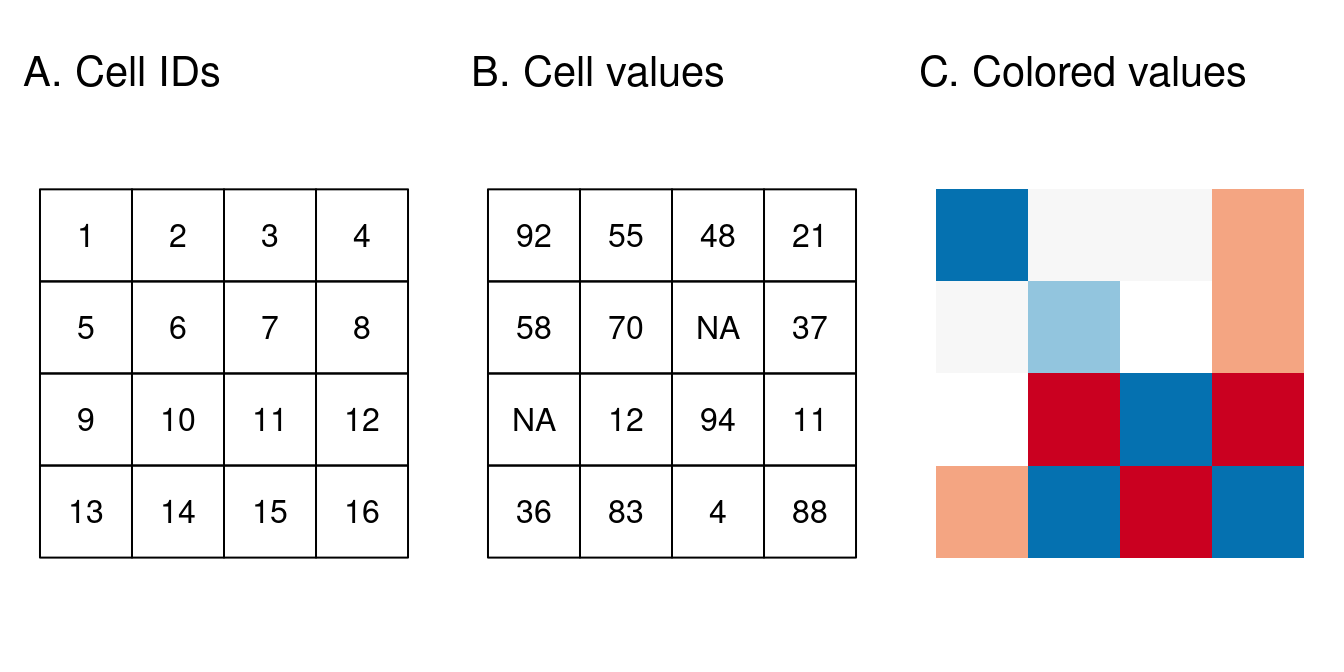
\includegraphics{images/raster-intro-plot1.png}

}

\caption{\label{fig-raster-intro-plot1}Raster data types: (A) cell IDs,
(B) cell values, (C) a colored raster map}

\end{figure}%

Raster maps usually represent continuous phenomena such as elevation,
temperature, population density, or spectral data. Discrete features
such as soil or land-cover classes can also be represented in the raster
data model. Both uses of raster datasets are illustrated in
Figure~\ref{fig-raster-intro-plot2}, which shows how the borders of
discrete features may become blurred in raster datasets. Depending on
the nature of the application, vector representations of discrete
features may be more suitable.

\begin{figure}

\centering{

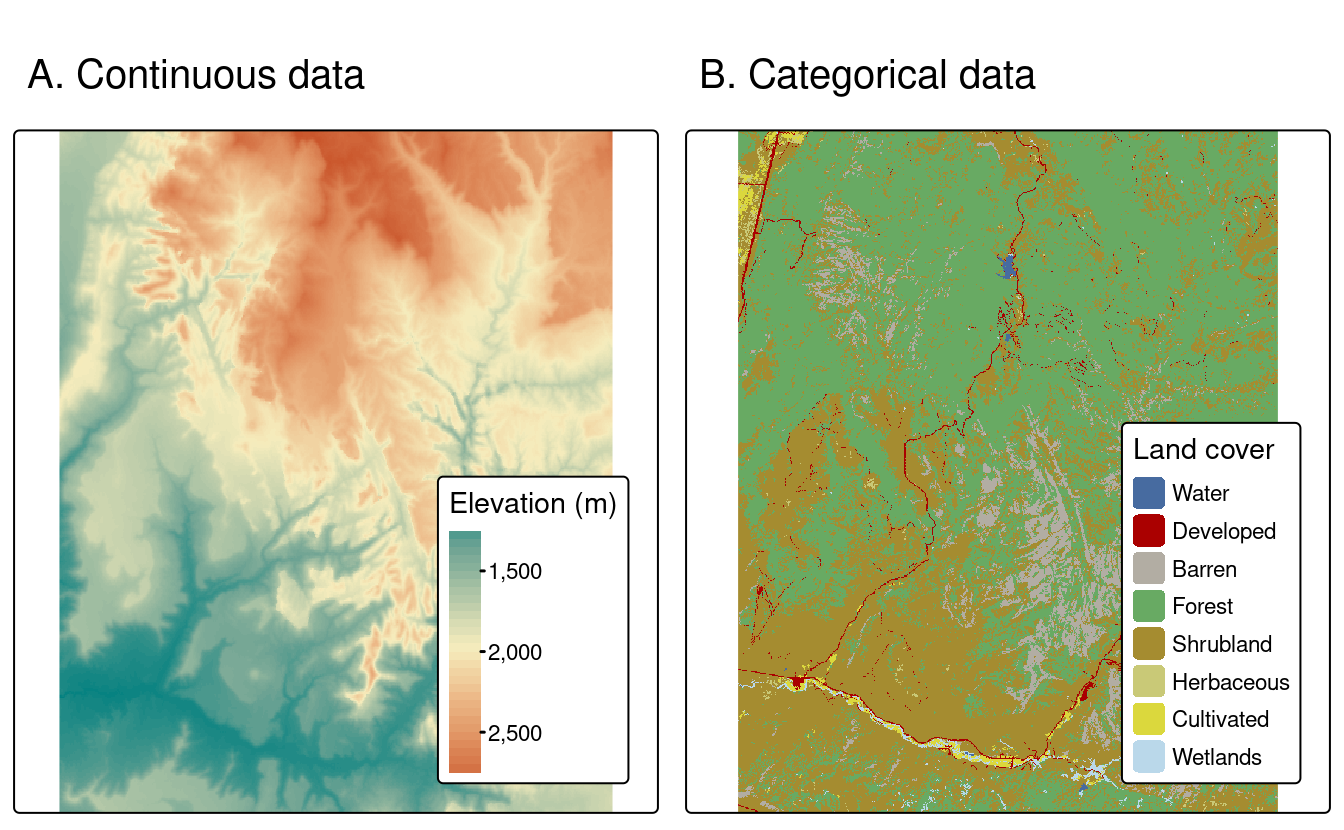
\includegraphics{images/raster-intro-plot2.png}

}

\caption{\label{fig-raster-intro-plot2}Examples of continuous and
categorical rasters}

\end{figure}%

As mentioned above, working with rasters in Python is less organized
around one comprehensive package as compared to the case for vector
layers and \textbf{geopandas}. Instead, several packages provide
alternative subsets of methods for working with raster data.

The two most notable approaches for working with rasters in Python are
provided by \textbf{rasterio} and \textbf{rioxarray} packages. As we
will see shortly, they differ in scope and underlying data models.
Specifically, \textbf{rasterio} represents rasters as \textbf{numpy}
arrays associated with a separate object holding the spatial metadata.
The \textbf{rioxarray} package, a wrapper of \textbf{rasterio}, however,
represents rasters with \textbf{xarray} `extended' arrays, which are an
extension of \textbf{numpy} array designed to hold axis labels and
attributes in the same object, together with the array of raster values.
Similar approaches are provided by less well-known
\textbf{xarray-spatial} and \textbf{geowombat} packages. Comparatively,
\textbf{rasterio} is more well-established, but it is more low-level
(which has both advantages and distadvantages).

All of the above-mentioned packages, however, are not exhaustive in the
same way \textbf{geopandas} is. For example, when working with
\textbf{rasterio}, more packages may be needed to accomplish common
tasks such as zonal statistics (package \textbf{rasterstats}) or
calculating topographic indices (package \textbf{richdem}).

In the following two sections, we introduce \textbf{rasterio}, which is
the raster-related package we are going to work with through the rest of
the book.

\subsection{\texorpdfstring{Using
\textbf{rasterio}}{Using rasterio}}\label{sec-using-rasterio}

To work with the \textbf{rasterio} package, we first need to import it.
Additionally, as the raster data is stored within \textbf{numpy} arrays,
we import the \textbf{numpy} package and make all its functions
accessible for effective data manipulation. Finally, we import the
\textbf{rasterio.plot} sub-module for its \texttt{rasterio.plot.show}
function that allows for quick visualization of rasters.

\begin{Shaded}
\begin{Highlighting}[]
\ImportTok{import}\NormalTok{ numpy }\ImportTok{as}\NormalTok{ np}
\ImportTok{import}\NormalTok{ rasterio}
\ImportTok{import}\NormalTok{ rasterio.plot}
\end{Highlighting}
\end{Shaded}

Rasters are typically imported from existing files. When working with
\textbf{rasterio}, importing a raster is actually a two-step process:

\begin{itemize}
\tightlist
\item
  First, we open a raster file `connection' using \texttt{rasterio.open}
\item
  Second, we read raster values from the connection using the
  \texttt{.read} method
\end{itemize}

This type of separation is analogous to basic Python functions for
reading from files, such as \texttt{open} and \texttt{.readline} to read
from a text file. The rationale is that we do not always want to read
all information from the file into memory, which is particularly
important as rasters size can be larger than RAM size. Accordingly, the
second step (\texttt{.read}) is selective, meaning that the user can
fine-tune the subset of values (bands, rows/columns, resolution, etc.)
that are actually being read. For example, we may want to read just one
raster band rather than reading all bands.

In the first step, we pass a file path to the \texttt{rasterio.open}
function to create a \texttt{DatasetReader} file connection, hereby
named \texttt{src}. For this example, we use a single-band raster
representing elevation in Zion National Park, stored in
\texttt{srtm.tif}.

\begin{Shaded}
\begin{Highlighting}[]
\NormalTok{src }\OperatorTok{=}\NormalTok{ rasterio.}\BuiltInTok{open}\NormalTok{(}\StringTok{\textquotesingle{}data/srtm.tif\textquotesingle{}}\NormalTok{)}
\NormalTok{src}
\end{Highlighting}
\end{Shaded}

\begin{verbatim}
<open DatasetReader name='data/srtm.tif' mode='r'>
\end{verbatim}

To get a first impression of the raster values, we can plot the raster
using the \texttt{rasterio.plot.show} function
(Figure~\ref{fig-rasterio-plot}):

\begin{Shaded}
\begin{Highlighting}[]
\NormalTok{rasterio.plot.show(src)}\OperatorTok{;}
\end{Highlighting}
\end{Shaded}

\begin{figure}[H]

\centering{

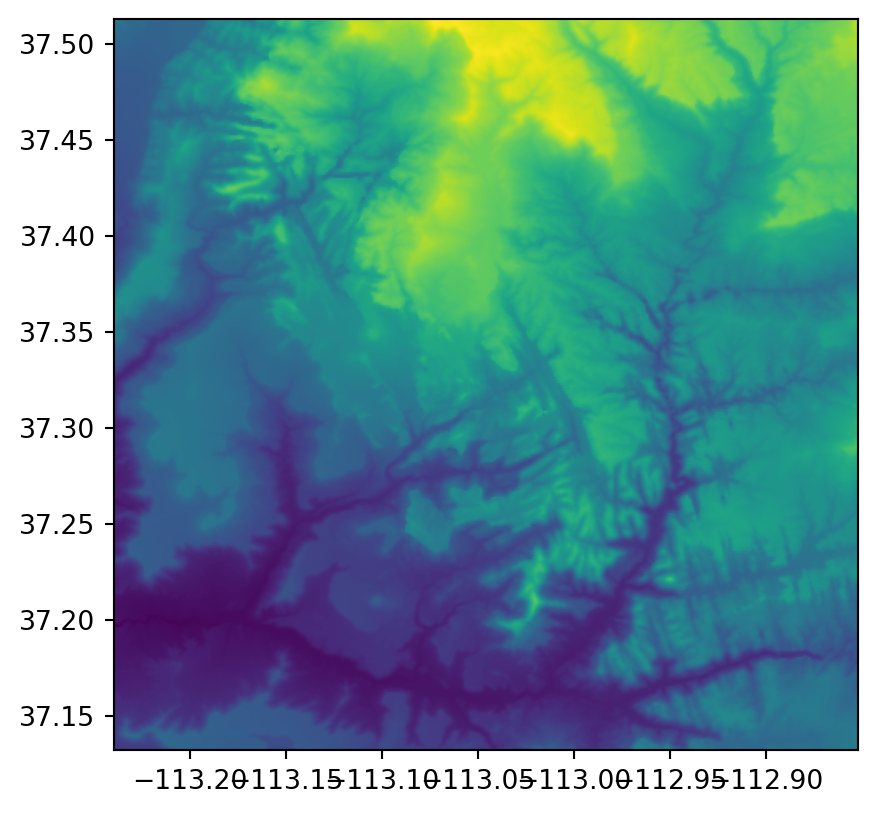
\includegraphics{01-spatial-data_files/figure-pdf/fig-rasterio-plot-output-1.pdf}

}

\caption{\label{fig-rasterio-plot}Basic plot of a raster, the data are
coming from a \textbf{rasterio} file connection}

\end{figure}%

The \texttt{DatasetReader} contains the raster metadata, that is, all of
the information other than the raster values. Let's examine it with the
\texttt{.meta} property.

\begin{Shaded}
\begin{Highlighting}[]
\NormalTok{src.meta}
\end{Highlighting}
\end{Shaded}

\begin{verbatim}
{'driver': 'GTiff',
 'dtype': 'uint16',
 'nodata': 65535.0,
 'width': 465,
 'height': 457,
 'count': 1,
 'crs': CRS.from_epsg(4326),
 'transform': Affine(0.0008333333332777796, 0.0, -113.23958321278403,
        0.0, -0.0008333333332777843, 37.512916763165805)}
\end{verbatim}

Namely, it allows us to see the following properties, which we will
elaborate on below, and in later chapters:

\begin{itemize}
\tightlist
\item
  \texttt{driver}---The raster file format (see
  Section~\ref{sec-data-output-raster})
\item
  \texttt{dtype}---Data type (see Table~\ref{tbl-numpy-data-types})
\item
  \texttt{nodata}---The value being used as `No Data' flag (see
  Section~\ref{sec-data-output-raster})
\item
  Dimensions:

  \begin{itemize}
  \tightlist
  \item
    \texttt{width}---Number of columns
  \item
    \texttt{height}---Number of rows
  \item
    \texttt{count}---Number of bands
  \end{itemize}
\item
  \texttt{crs}---Coordinate reference system (see
  Section~\ref{sec-querying-and-setting-coordinate-systems})
\item
  \texttt{transform}---The raster affine transformation matrix
\end{itemize}

The last item (i.e., \texttt{transform}) deserves more attention. To
position a raster in geographical space, in addition to the CRS, we must
specify the raster \emph{origin} (\(x_{min}\), \(y_{max}\)) and
resolution (\(delta_{x}\), \(delta_{y}\)). In the transformation matrix
notation, assuming a regular grid, these data items are stored as
follows:

\begin{Shaded}
\begin{Highlighting}[]
\NormalTok{Affine(delta\_x, 0.0, x\_min,}
\NormalTok{       0.0, delta\_y, y\_max)}
\end{Highlighting}
\end{Shaded}

Note that, by convention, raster y-axis origin is set to the maximum
value (\(y_{max}\)) rather than the minimum, and, accordingly, the
y-axis resolution (\(delta_{y}\)) is negative. In other words, since the
origin is in the \emph{top}-left corner, advancing along the y-axis is
done through negative steps (downwards).

In the second step, the \texttt{.read} method of the
\texttt{DatasetReader} is used to read the actual raster values.
Importantly, we can read:

\begin{itemize}
\tightlist
\item
  All layers (as in \texttt{.read()})
\item
  A particular layer, passing a numeric index (as in \texttt{.read(1)})
\item
  A subset of layers, passing a \texttt{list} of indices (as in
  \texttt{.read({[}1,2{]})})
\end{itemize}

Note that the layer indices start from \texttt{1}, contrary to the
Python convention of the first index being \texttt{0}.

The object returned by \texttt{.read} is a \textbf{numpy} array (Harris
et al. 2020), with either two or three dimensions:

\begin{itemize}
\tightlist
\item
  \emph{Three} dimensions, when reading more than one layer (e.g.,
  \texttt{.read()} or \texttt{.read({[}1,2{]})}). In such case, the
  dimensions pattern is \texttt{(layers,\ rows,\ columns)}
\item
  \emph{Two} dimensions, when reading one specific layer (e.g.,
  \texttt{.read(1)}). In such case, the dimensions pattern is
  \texttt{(rows,\ columns)}
\end{itemize}

Let's read the first (and only) layer from the \texttt{srtm.tif} raster,
using the file connection object \texttt{src} and the \texttt{.read}
method.

\begin{Shaded}
\begin{Highlighting}[]
\NormalTok{src.read(}\DecValTok{1}\NormalTok{)}
\end{Highlighting}
\end{Shaded}

\begin{verbatim}
array([[1728, 1718, 1715, ..., 2654, 2674, 2685],
       [1737, 1727, 1717, ..., 2649, 2677, 2693],
       [1739, 1734, 1727, ..., 2644, 2672, 2695],
       ...,
       [1326, 1328, 1329, ..., 1777, 1778, 1775],
       [1320, 1323, 1326, ..., 1771, 1770, 1772],
       [1319, 1319, 1322, ..., 1768, 1770, 1772]], dtype=uint16)
\end{verbatim}

The result is a two-dimensional \textbf{numpy} array where each value
represents the elevation of the corresponding pixel.

The relation between a \textbf{rasterio} file connection and the derived
properties is summarized in Figure~\ref{fig-rasterio-structure}. The
file connection (created with \texttt{rasterio.open}) gives access to
the two components of raster data: the metadata (via the \texttt{.meta}
property) and the values (via the \texttt{.read} method).

\begin{figure}

\centering{

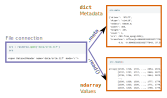
\includegraphics{index_files/mediabag/images/rasterio-structure.pdf}

}

\caption{\label{fig-rasterio-structure}A \textbf{rasterio} file
connection and its derived components, the metadata and the raster
values}

\end{figure}%

\subsection{Raster from scratch}\label{sec-raster-from-scratch}

In this section, we are going to demonstrate the creation of rasters
from scratch. We will construct two small rasters, \texttt{elev} and
\texttt{grain}, which we will use in examples later in the book. Unlike
creating a vector layer (see
Section~\ref{sec-vector-layer-from-scratch}), creating a raster from
scratch is rarely needed in practice because aligning a raster with the
proper spatial extent is challenging to do programmatically
(`georeferencing' tools in GIS software are a better fit for the job).
Nevertheless, the examples will be helpful to become more familiar with
the \textbf{rasterio} data structures.

Conceptually, a raster is an array combined with georeferencing
information, whereas the latter comprises:

\begin{itemize}
\tightlist
\item
  A transformation matrix, containing the origin and resolution, thus
  linking pixel indices with coordinates in a particular coordinate
  system
\item
  A CRS definition, specifying the association of that coordinate system
  with the surface of the earth (optional)
\end{itemize}

Therefore, to create a raster, we first need to have an array with the
values, and then supplement it with the georeferencing information.
Let's create the arrays \texttt{elev} and \texttt{grain}. The
\texttt{elev} array is a \(6 \times 6\) array with sequential values
from \texttt{1} to \texttt{36}. It can be created as follows using the
\texttt{np.arange} function and \texttt{.reshape} method from
\textbf{numpy}.

\begin{Shaded}
\begin{Highlighting}[]
\NormalTok{elev }\OperatorTok{=}\NormalTok{ np.arange(}\DecValTok{1}\NormalTok{, }\DecValTok{37}\NormalTok{, dtype}\OperatorTok{=}\NormalTok{np.uint8).reshape(}\DecValTok{6}\NormalTok{, }\DecValTok{6}\NormalTok{)}
\NormalTok{elev}
\end{Highlighting}
\end{Shaded}

\begin{verbatim}
array([[ 1,  2,  3,  4,  5,  6],
       [ 7,  8,  9, 10, 11, 12],
       [13, 14, 15, 16, 17, 18],
       [19, 20, 21, 22, 23, 24],
       [25, 26, 27, 28, 29, 30],
       [31, 32, 33, 34, 35, 36]], dtype=uint8)
\end{verbatim}

The \texttt{grain} array represents a categorical raster with values
\texttt{0}, \texttt{1}, \texttt{2}, corresponding to categories `clay',
`silt', `sand', respectively. We will create it from a specific
arrangement of pixel values, using \textbf{numpy}'s \texttt{np.array}
and \texttt{.reshape}.

\begin{Shaded}
\begin{Highlighting}[]
\NormalTok{v }\OperatorTok{=}\NormalTok{ [}
  \DecValTok{1}\NormalTok{, }\DecValTok{0}\NormalTok{, }\DecValTok{1}\NormalTok{, }\DecValTok{2}\NormalTok{, }\DecValTok{2}\NormalTok{, }\DecValTok{2}\NormalTok{, }
  \DecValTok{0}\NormalTok{, }\DecValTok{2}\NormalTok{, }\DecValTok{0}\NormalTok{, }\DecValTok{0}\NormalTok{, }\DecValTok{2}\NormalTok{, }\DecValTok{1}\NormalTok{, }
  \DecValTok{0}\NormalTok{, }\DecValTok{2}\NormalTok{, }\DecValTok{2}\NormalTok{, }\DecValTok{0}\NormalTok{, }\DecValTok{0}\NormalTok{, }\DecValTok{2}\NormalTok{, }
  \DecValTok{0}\NormalTok{, }\DecValTok{0}\NormalTok{, }\DecValTok{1}\NormalTok{, }\DecValTok{1}\NormalTok{, }\DecValTok{1}\NormalTok{, }\DecValTok{1}\NormalTok{, }
  \DecValTok{1}\NormalTok{, }\DecValTok{1}\NormalTok{, }\DecValTok{1}\NormalTok{, }\DecValTok{2}\NormalTok{, }\DecValTok{1}\NormalTok{, }\DecValTok{1}\NormalTok{, }
  \DecValTok{2}\NormalTok{, }\DecValTok{1}\NormalTok{, }\DecValTok{2}\NormalTok{, }\DecValTok{2}\NormalTok{, }\DecValTok{0}\NormalTok{, }\DecValTok{2}
\NormalTok{]}
\NormalTok{grain }\OperatorTok{=}\NormalTok{ np.array(v, dtype}\OperatorTok{=}\NormalTok{np.uint8).reshape(}\DecValTok{6}\NormalTok{, }\DecValTok{6}\NormalTok{)}
\NormalTok{grain}
\end{Highlighting}
\end{Shaded}

\begin{verbatim}
array([[1, 0, 1, 2, 2, 2],
       [0, 2, 0, 0, 2, 1],
       [0, 2, 2, 0, 0, 2],
       [0, 0, 1, 1, 1, 1],
       [1, 1, 1, 2, 1, 1],
       [2, 1, 2, 2, 0, 2]], dtype=uint8)
\end{verbatim}

Note that, in both cases, we are using the \texttt{uint8} (unsigned
integer in 8 bits, i.e., \texttt{0-255}) data type, which is sufficient
to represent all possible values of the given rasters (see
Table~\ref{tbl-numpy-data-types}). This is the recommended approach for
a minimal memory footprint.

What is missing now is the georeferencing information (see
Section~\ref{sec-using-rasterio}). In this case, since the rasters are
arbitrary, we also set up an arbitrary transformation matrix, where:

\begin{itemize}
\tightlist
\item
  The origin (\(x_{min}\), \(y_{max}\)) is at \texttt{-1.5,1.5}
\item
  The raster resolution (\(delta_{x}\), \(delta_{y}\)) is
  \texttt{0.5,-0.5}
\end{itemize}

We can add this information using
\texttt{rasterio.transform.from\_origin}, and specifying \texttt{west},
\texttt{north}, \texttt{xsize}, and \texttt{ysize} parameters. The
resulting transformation matrix object is hereby named
\texttt{new\_transform}.

\begin{Shaded}
\begin{Highlighting}[]
\NormalTok{new\_transform }\OperatorTok{=}\NormalTok{ rasterio.transform.from\_origin(}
\NormalTok{    west}\OperatorTok{={-}}\FloatTok{1.5}\NormalTok{, }
\NormalTok{    north}\OperatorTok{=}\FloatTok{1.5}\NormalTok{, }
\NormalTok{    xsize}\OperatorTok{=}\FloatTok{0.5}\NormalTok{, }
\NormalTok{    ysize}\OperatorTok{=}\FloatTok{0.5}
\NormalTok{)}
\NormalTok{new\_transform}
\end{Highlighting}
\end{Shaded}

\begin{verbatim}
Affine(0.5, 0.0, -1.5,
       0.0, -0.5, 1.5)
\end{verbatim}

Note that, confusingly, \(delta_{y}\) (i.e., \texttt{ysize}) is defined
in \texttt{rasterio.transform.from\_origin} using a positive value
(\texttt{0.5}), even though it is, in fact, negative (\texttt{-0.5}).

The raster can now be plotted in its coordinate system, passing the
array \texttt{elev} along with the transformation matrix
\texttt{new\_transform} to \texttt{rasterio.plot.show}
(Figure~\ref{fig-rasterio-plot-elev}).

\begin{Shaded}
\begin{Highlighting}[]
\NormalTok{rasterio.plot.show(elev, transform}\OperatorTok{=}\NormalTok{new\_transform)}\OperatorTok{;}
\end{Highlighting}
\end{Shaded}

\begin{figure}[H]

\centering{

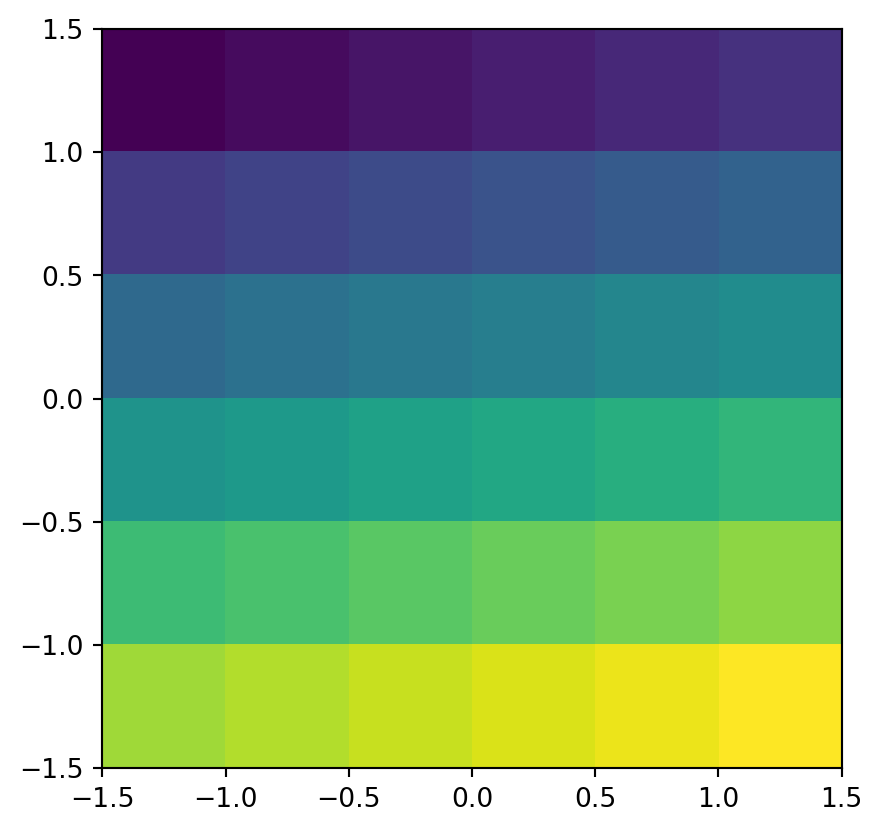
\includegraphics{01-spatial-data_files/figure-pdf/fig-rasterio-plot-elev-output-1.pdf}

}

\caption{\label{fig-rasterio-plot-elev}Plot of the \texttt{elev} raster,
a minimal example of a continuous raster, created from scratch}

\end{figure}%

The \texttt{grain} raster can be plotted the same way, as we are going
to use the same transformation matrix for it as well
(Figure~\ref{fig-rasterio-plot-grain}).

\begin{Shaded}
\begin{Highlighting}[]
\NormalTok{rasterio.plot.show(grain, transform}\OperatorTok{=}\NormalTok{new\_transform)}\OperatorTok{;}
\end{Highlighting}
\end{Shaded}

\begin{figure}[H]

\centering{

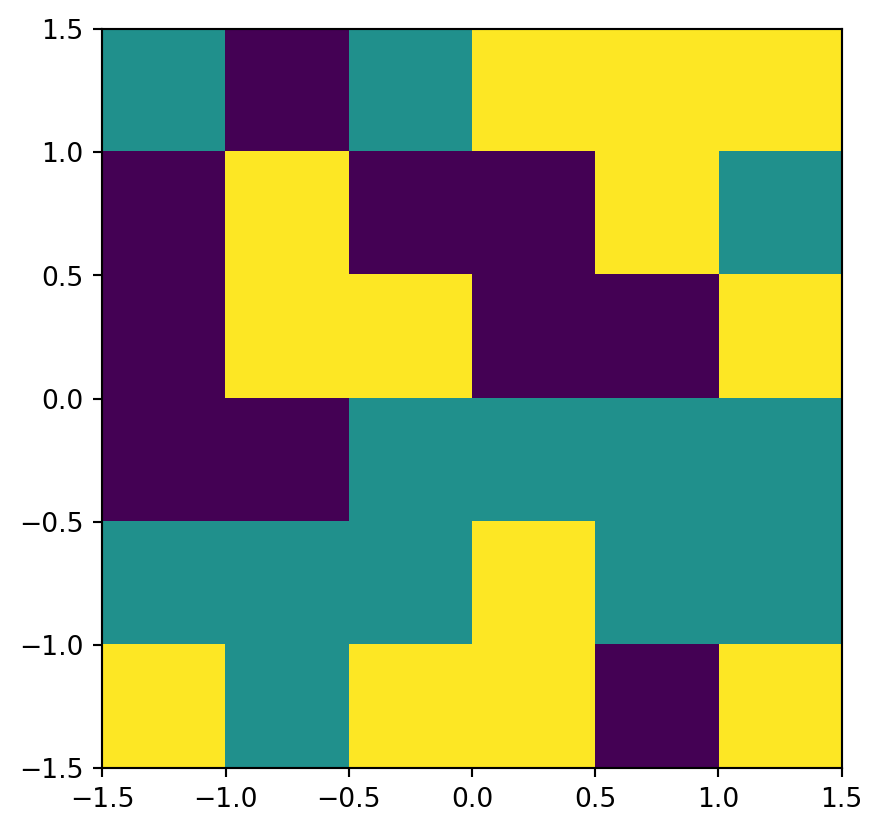
\includegraphics{01-spatial-data_files/figure-pdf/fig-rasterio-plot-grain-output-1.pdf}

}

\caption{\label{fig-rasterio-plot-grain}Plot of the \texttt{grain}
raster, a minimal example of a categorical raster, created from scratch}

\end{figure}%

At this point, we have two rasters, each composed of an array and
related transformation matrix. We can work with the raster using
\textbf{rasterio} by:

\begin{itemize}
\tightlist
\item
  Passing the transformation matrix wherever actual raster pixel
  coordinates are important (such as in function
  \texttt{rasterio.plot.show} above)
\item
  Keeping in mind that any other layer we use in the analysis is in the
  same CRS
\end{itemize}

Finally, to export the raster for permanent storage, along with the
spatial metadata, we need to go through the following steps:

\begin{enumerate}
\def\labelenumi{\arabic{enumi}.}
\tightlist
\item
  Create a raster file connection (where we set the transform and the
  CRS, among other settings)
\item
  Write the array with raster values into the connection
\item
  Close the connection
\end{enumerate}

Don't worry if the code below is unclear; the concepts related to
writing raster data to file will be explained in
Section~\ref{sec-data-output-raster}. For now, for completeness, and
also to use these rasters in subsequent chapters without having to
re-create them from scratch, we just provide the code for exporting the
\texttt{elev} and \texttt{grain} rasters into the \texttt{output}
directory. In the case of \texttt{elev}, we do it as follows with the
\texttt{rasterio.open}, \texttt{.write}, and \texttt{.close} functions
and methods of the \textbf{rasterio} package.

\begin{Shaded}
\begin{Highlighting}[]
\NormalTok{new\_dataset }\OperatorTok{=}\NormalTok{ rasterio.}\BuiltInTok{open}\NormalTok{(}
    \StringTok{\textquotesingle{}output/elev.tif\textquotesingle{}}\NormalTok{, }\StringTok{\textquotesingle{}w\textquotesingle{}}\NormalTok{, }
\NormalTok{    driver}\OperatorTok{=}\StringTok{\textquotesingle{}GTiff\textquotesingle{}}\NormalTok{,}
\NormalTok{    height}\OperatorTok{=}\NormalTok{elev.shape[}\DecValTok{0}\NormalTok{],}
\NormalTok{    width}\OperatorTok{=}\NormalTok{elev.shape[}\DecValTok{1}\NormalTok{],}
\NormalTok{    count}\OperatorTok{=}\DecValTok{1}\NormalTok{,}
\NormalTok{    dtype}\OperatorTok{=}\NormalTok{elev.dtype,}
\NormalTok{    crs}\OperatorTok{=}\DecValTok{4326}\NormalTok{,}
\NormalTok{    transform}\OperatorTok{=}\NormalTok{new\_transform}
\NormalTok{)}
\NormalTok{new\_dataset.write(elev, }\DecValTok{1}\NormalTok{)}
\NormalTok{new\_dataset.close()}
\end{Highlighting}
\end{Shaded}

Note that the CRS we (arbitrarily) set for the \texttt{elev} raster is
WGS84, defined using \texttt{crs=4326} according to the EPSG code.

Exporting the \texttt{grain} raster is done in the same way, with the
only differences being the file name and the array we write into the
connection.

\begin{Shaded}
\begin{Highlighting}[]
\NormalTok{new\_dataset }\OperatorTok{=}\NormalTok{ rasterio.}\BuiltInTok{open}\NormalTok{(}
    \StringTok{\textquotesingle{}output/grain.tif\textquotesingle{}}\NormalTok{, }\StringTok{\textquotesingle{}w\textquotesingle{}}\NormalTok{, }
\NormalTok{    driver}\OperatorTok{=}\StringTok{\textquotesingle{}GTiff\textquotesingle{}}\NormalTok{,}
\NormalTok{    height}\OperatorTok{=}\NormalTok{grain.shape[}\DecValTok{0}\NormalTok{],}
\NormalTok{    width}\OperatorTok{=}\NormalTok{grain.shape[}\DecValTok{1}\NormalTok{],}
\NormalTok{    count}\OperatorTok{=}\DecValTok{1}\NormalTok{,}
\NormalTok{    dtype}\OperatorTok{=}\NormalTok{grain.dtype,}
\NormalTok{    crs}\OperatorTok{=}\DecValTok{4326}\NormalTok{,}
\NormalTok{    transform}\OperatorTok{=}\NormalTok{new\_transform}
\NormalTok{)}
\NormalTok{new\_dataset.write(grain, }\DecValTok{1}\NormalTok{)}
\NormalTok{new\_dataset.close()}
\end{Highlighting}
\end{Shaded}

As a result, the files \texttt{elev.tif} and \texttt{grain.tif} are
written into the \texttt{output} directory. We are going to use these
small raster files later on in the examples (for example,
Section~\ref{sec-raster-subsetting}).

Note that the transform matrices and dimensions of \texttt{elev} and
\texttt{grain} are identical. This means that the rasters are
overlapping, and can be combined into one two-band raster, processed in
raster algebra operations (Section~\ref{sec-map-algebra}), etc.

\section{Coordinate Reference
Systems}\label{sec-coordinate-reference-systems-intro}

Vector and raster spatial data types share concepts intrinsic to spatial
data. Perhaps the most fundamental of these is the Coordinate Reference
System (CRS), which defines how the spatial elements of the data relate
to the surface of the Earth (or other bodies). CRSs are either
geographic or projected, as introduced at the beginning of this chapter
(Section~\ref{sec-vector-data}). This section explains each type, laying
the foundations for Chapter~\ref{sec-reproj-geo-data}, which provides a
deep dive into setting, transforming, and querying CRSs.

\subsection{Geographic coordinate
systems}\label{geographic-coordinate-systems}

Geographic coordinate systems identify any location on the Earth's
surface using two values---longitude and latitude (see left panel of
Figure~\ref{fig-zion-crs}). Longitude is a location in the East-West
direction in angular distance from the Prime Meridian plane, while
latitude is an angular distance North or South of the equatorial plane.
Distances in geographic CRSs are therefore not measured in meters. This
has important consequences, as demonstrated in
Chapter~\ref{sec-reproj-geo-data}.

A spherical or ellipsoidal surface represents the surface of the Earth
in geographic coordinate systems. Spherical models assume that the Earth
is a perfect sphere of a given radius---they have the advantage of
simplicity, but, at the same time, they are inaccurate: the Earth is not
a sphere! Ellipsoidal models are defined by two parameters: the
equatorial radius and the polar radius. These are suitable because the
Earth is compressed: the equatorial radius is around 11.5 \(km\) longer
than the polar radius. The Earth is not an ellipsoid either, but it is a
better approximation than a sphere.

Ellipsoids are part of a broader component of CRSs: the datum. It
contains information on what ellipsoid to use and the precise
relationship between the Cartesian coordinates and location on the
Earth's surface. There are two types of datum---geocentric (such as
WGS84) and local (such as NAD83). You can see examples of these two
types of datums in Figure~\ref{fig-geocentric-vs-local}. Black lines
represent a geocentric datum, whose center is located in the Earth's
center of gravity and is not optimized for a specific location. In a
local datum, shown as a purple dashed line, the ellipsoidal surface is
shifted to align with the surface at a particular location. These allow
local variations on Earth's surface, such as large mountain ranges, to
be accounted for in a local CRS. This can be seen in
Figure~\ref{fig-geocentric-vs-local}, where the local datum is fitted to
the area of Philippines, but is misaligned with most of the rest of the
planet's surface. Both datums in Figure~\ref{fig-geocentric-vs-local}
are put on top of a geoid---a model of global mean sea level.

\begin{figure}

\centering{

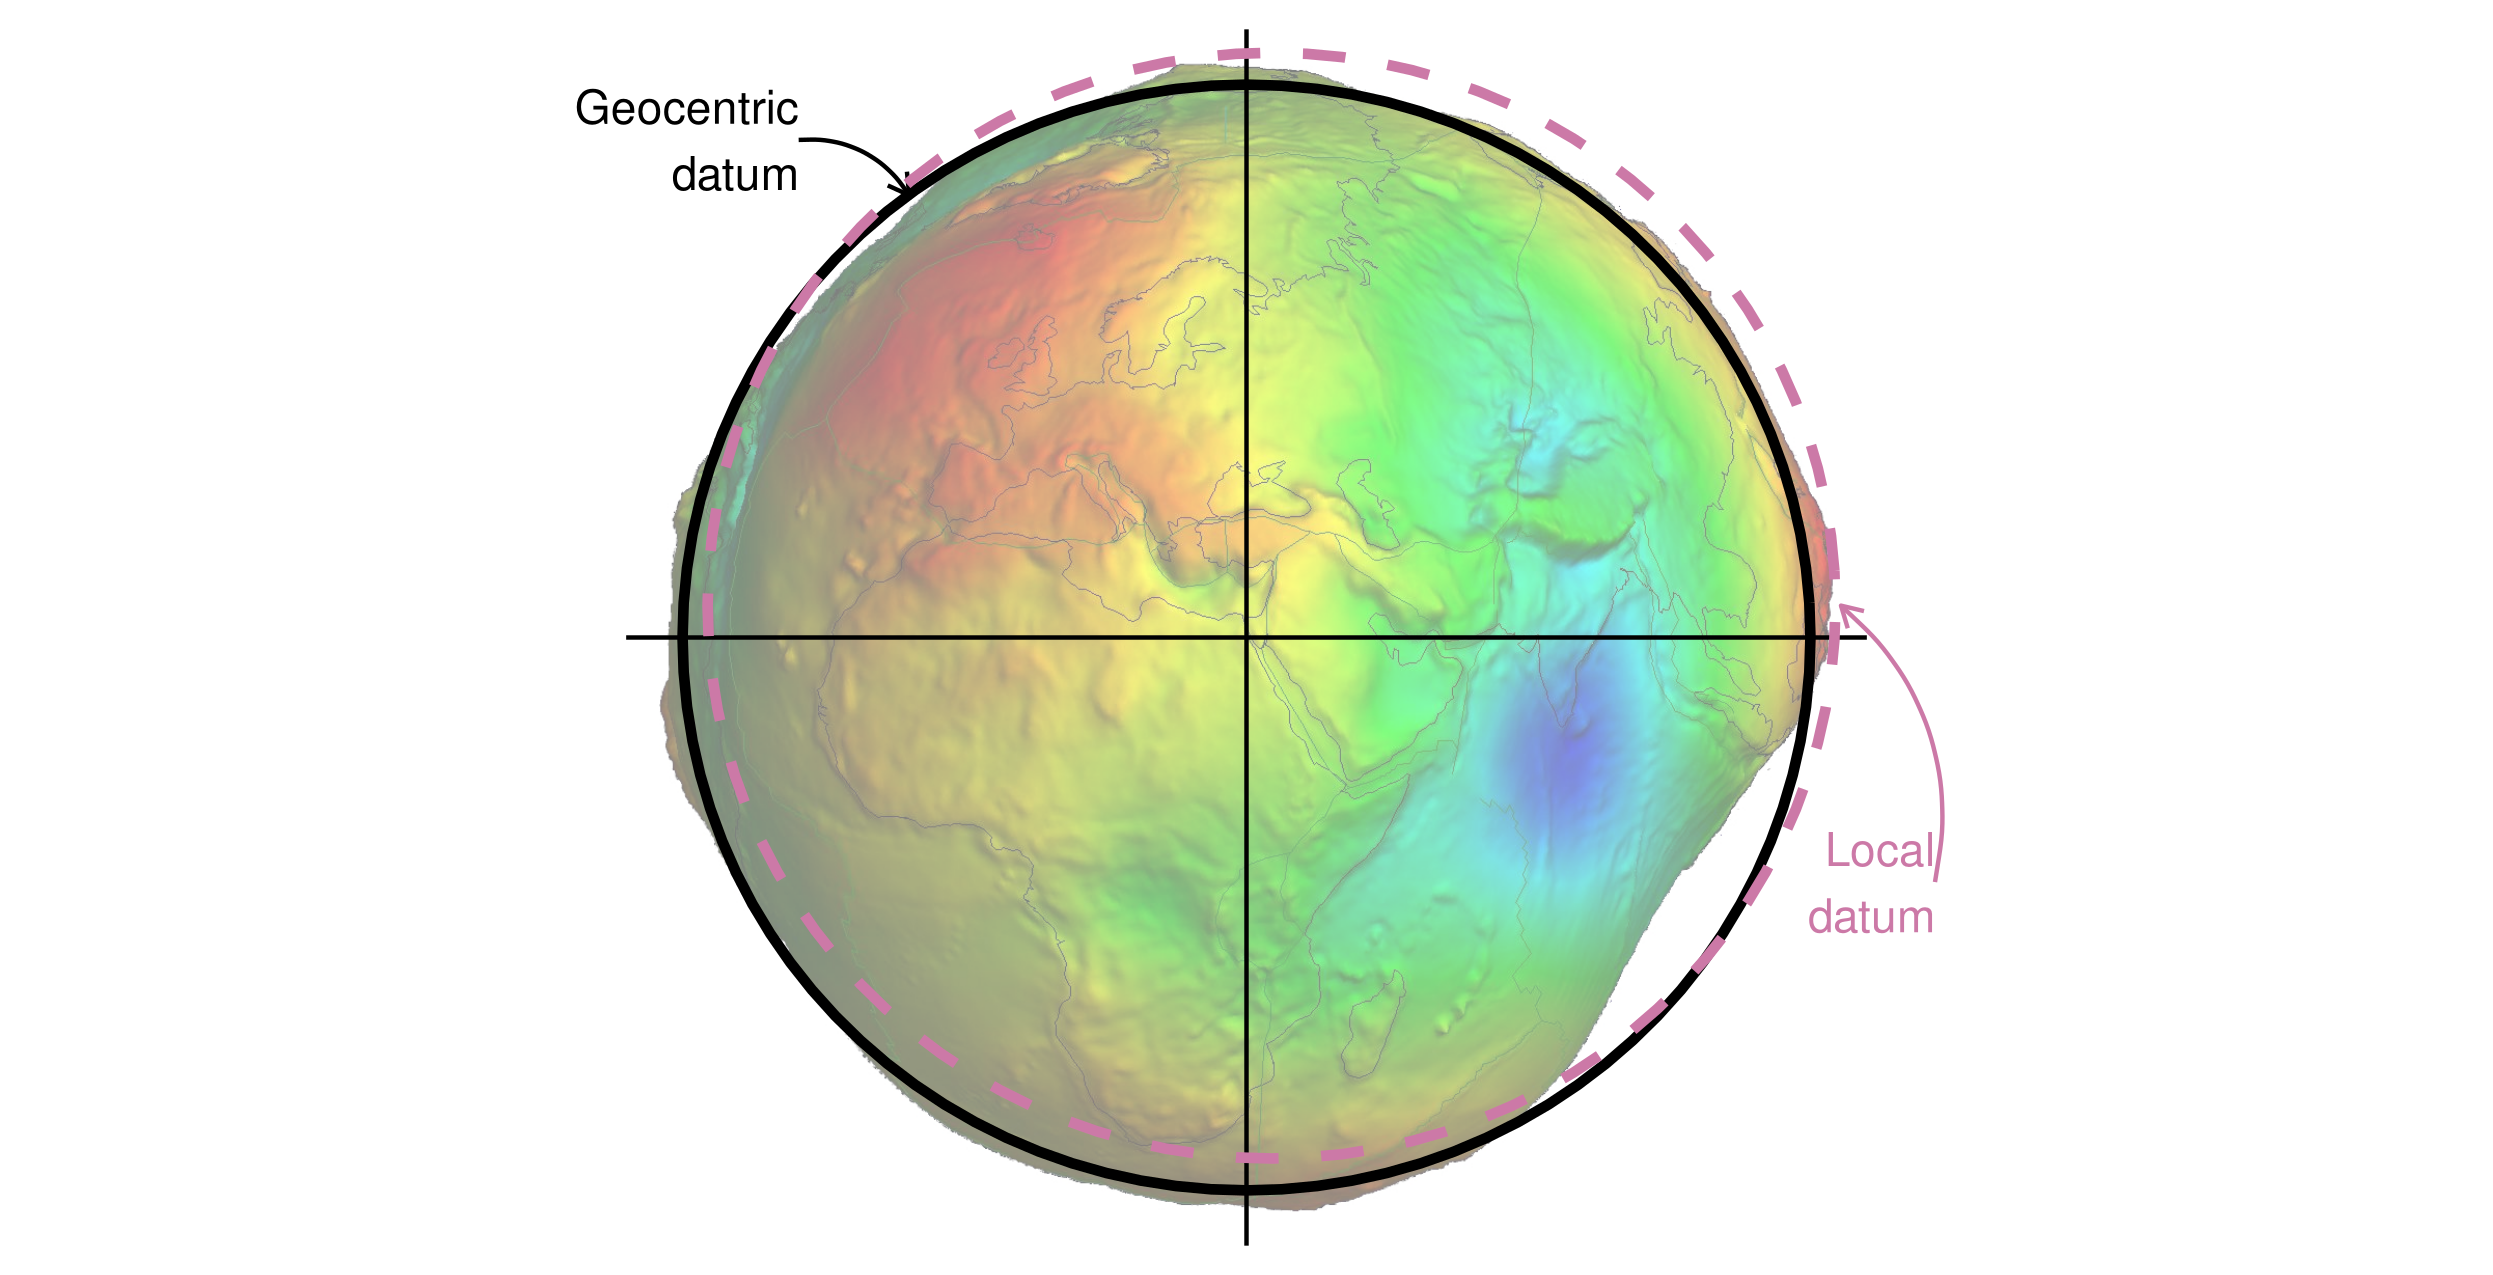
\includegraphics{images/geocompr_02_datum_fig.png}

}

\caption{\label{fig-geocentric-vs-local}Geocentric and local geodetic
datums shown on top of a geoid (in false color and the vertical
exaggeration by 10,000 scale factor). Image of the geoid is adapted from
the work of Ince et al. (2019).}

\end{figure}%

\subsection{Projected coordinate reference
systems}\label{sec-projected-coordinate-reference-systems}

All projected CRSs are based on a geographic CRS, described in the
previous section, and rely on map projections to convert the
three-dimensional surface of the Earth into Easting and Northing (x and
y) values in a projected CRS. Projected CRSs are based on Cartesian
coordinates on an implicitly flat surface (see right panel of
Figure~\ref{fig-zion-crs}). They have an origin, x and y axes, and a
linear unit of measurement such as meters.

This transition cannot be done without adding some deformations.
Therefore, some properties of the Earth's surface are distorted in this
process, such as area, direction, distance, and shape. A projected
coordinate system can preserve only one or two of those properties.
Projections are often named based on a property they preserve:
equal-area preserves area, azimuthal preserves direction, equidistant
preserves distance, and conformal preserves local shape.

There are three main groups of projection types: conic, cylindrical, and
planar (azimuthal). In a conic projection, the Earth's surface is
projected onto a cone along a single line of tangency or two lines of
tangency. Distortions are minimized along the tangency lines and rise
with the distance from those lines in this projection. Therefore, it is
best suited for maps of mid-latitude areas. A cylindrical projection
maps the surface onto a cylinder. This projection could also be created
by touching the Earth's surface along a single line of tangency or two
lines of tangency. Cylindrical projections are used most often when
mapping the entire world. A planar projection projects data onto a flat
surface touching the globe at a point or along a line of tangency. It is
typically used in mapping polar regions.

\subsection{CRS in Python}\label{sec-crs-python}

Like most open-source geospatial software, the \textbf{geopandas} and
\textbf{rasterio} packages use the PROJ software for CRS definition and
calculations. The \textbf{pyproj} package is a low-level interface to
PROJ. Using its functions, such as \texttt{get\_codes} and
\texttt{from\_epsg}, we can examine the list of projections supported by
PROJ.

\begin{Shaded}
\begin{Highlighting}[]
\ImportTok{import}\NormalTok{ pyproj}
\NormalTok{epsg\_codes }\OperatorTok{=}\NormalTok{ pyproj.get\_codes(}\StringTok{\textquotesingle{}EPSG\textquotesingle{}}\NormalTok{, }\StringTok{\textquotesingle{}CRS\textquotesingle{}}\NormalTok{)  }\CommentTok{\#\# Supported EPSG codes}
\NormalTok{epsg\_codes[:}\DecValTok{5}\NormalTok{]  }\CommentTok{\#\# Print first five supported EPSG codes}
\end{Highlighting}
\end{Shaded}

\begin{verbatim}
['10150', '10151', '10156', '10157', '10158']
\end{verbatim}

\begin{Shaded}
\begin{Highlighting}[]
\NormalTok{pyproj.CRS.from\_epsg(}\DecValTok{4326}\NormalTok{)  }\CommentTok{\#\# Printout of WGS84 CRS (EPSG:4326)}
\end{Highlighting}
\end{Shaded}

\begin{verbatim}
<Geographic 2D CRS: EPSG:4326>
Name: WGS 84
Axis Info [ellipsoidal]:
- Lat[north]: Geodetic latitude (degree)
- Lon[east]: Geodetic longitude (degree)
Area of Use:
- name: World.
- bounds: (-180.0, -90.0, 180.0, 90.0)
Datum: World Geodetic System 1984 ensemble
- Ellipsoid: WGS 84
- Prime Meridian: Greenwich
\end{verbatim}

A quick summary of different projections, their types, properties, and
suitability can be found at \url{https://www.geo-projections.com/}. We
will expand on CRSs and explain how to project from one CRS to another
in Chapter~\ref{sec-reproj-geo-data}. But, for now, it is sufficient to
know:

\begin{itemize}
\tightlist
\item
  That coordinate systems are a key component of geographic objects
\item
  Knowing which CRS your data is in, and whether it is in geographic
  (lon/lat) or projected (typically meters), is important and has
  consequences for how Python handles spatial and geometry operations
\item
  CRSs of \textbf{geopandas} (vector layer or geometry column) and
  \textbf{rasterio} (raster) objects can be queried with the
  \texttt{.crs} property
\end{itemize}

Here is a demonstration of the last bullet point, where we import a
vector layer and figure out its CRS (in this case, a projected CRS,
namely UTM Zone 12) using the \texttt{.crs} property.

\begin{Shaded}
\begin{Highlighting}[]
\NormalTok{zion }\OperatorTok{=}\NormalTok{ gpd.read\_file(}\StringTok{\textquotesingle{}data/zion.gpkg\textquotesingle{}}\NormalTok{)}
\NormalTok{zion.crs}
\end{Highlighting}
\end{Shaded}

\begin{verbatim}
<Bound CRS: PROJCS["UTM Zone 12, Northern Hemisphere",GEOGCS[" ...>
Name: UTM Zone 12, Northern Hemisphere
Axis Info [cartesian]:
- [east]: Easting (Meter)
- [north]: Northing (Meter)
Area of Use:
- undefined
Coordinate Operation:
- name: Transformation from GRS 1980(IUGG, 1980) to WGS84
- method: Position Vector transformation (geog2D domain)
Datum: unknown
- Ellipsoid: GRS80
- Prime Meridian: Greenwich
Source CRS: UTM Zone 12, Northern Hemisphere
\end{verbatim}

We can also illustrate the difference between a geographic and a
projected CRS by plotting the \texttt{zion} data in both CRSs
(Figure~\ref{fig-zion-crs}). Note that we are using the \texttt{.grid}
method of \textbf{matplotlib} to draw grid lines on top of the plot.

\begin{Shaded}
\begin{Highlighting}[]
\CommentTok{\# WGS84}
\NormalTok{zion.to\_crs(}\DecValTok{4326}\NormalTok{).plot(edgecolor}\OperatorTok{=}\StringTok{\textquotesingle{}black\textquotesingle{}}\NormalTok{, color}\OperatorTok{=}\StringTok{\textquotesingle{}lightgrey\textquotesingle{}}\NormalTok{).grid()}
\CommentTok{\# NAD83 / UTM zone 12N}
\NormalTok{zion.plot(edgecolor}\OperatorTok{=}\StringTok{\textquotesingle{}black\textquotesingle{}}\NormalTok{, color}\OperatorTok{=}\StringTok{\textquotesingle{}lightgrey\textquotesingle{}}\NormalTok{).grid()}\OperatorTok{;}
\end{Highlighting}
\end{Shaded}

\begin{figure}

\begin{minipage}{0.50\linewidth}

\centering{

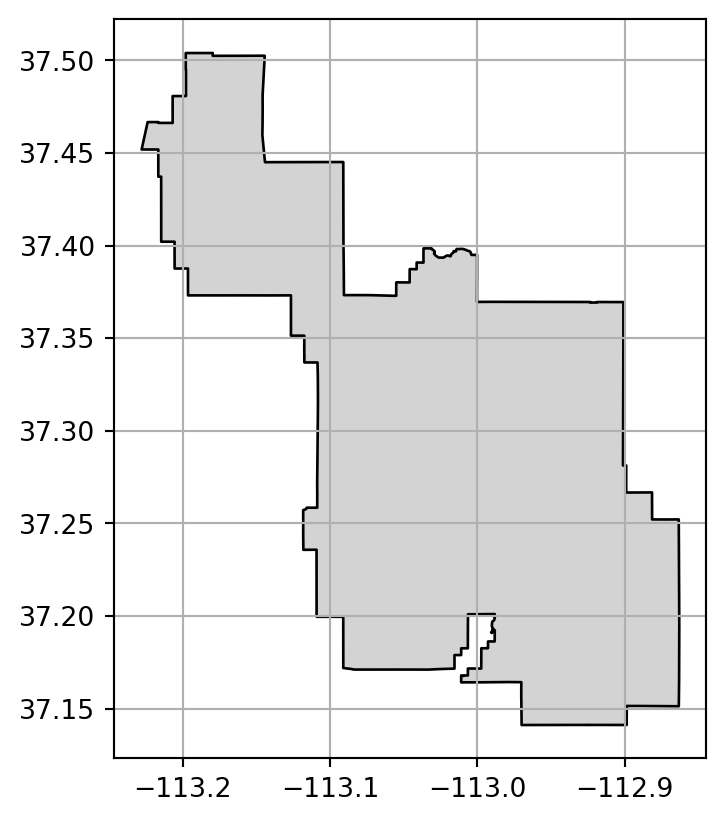
\includegraphics{01-spatial-data_files/figure-pdf/fig-zion-crs-output-1.pdf}

}

\subcaption{\label{fig-zion-crs-1}Geographic (WGS84)}

\end{minipage}%
%
\begin{minipage}{0.50\linewidth}

\centering{

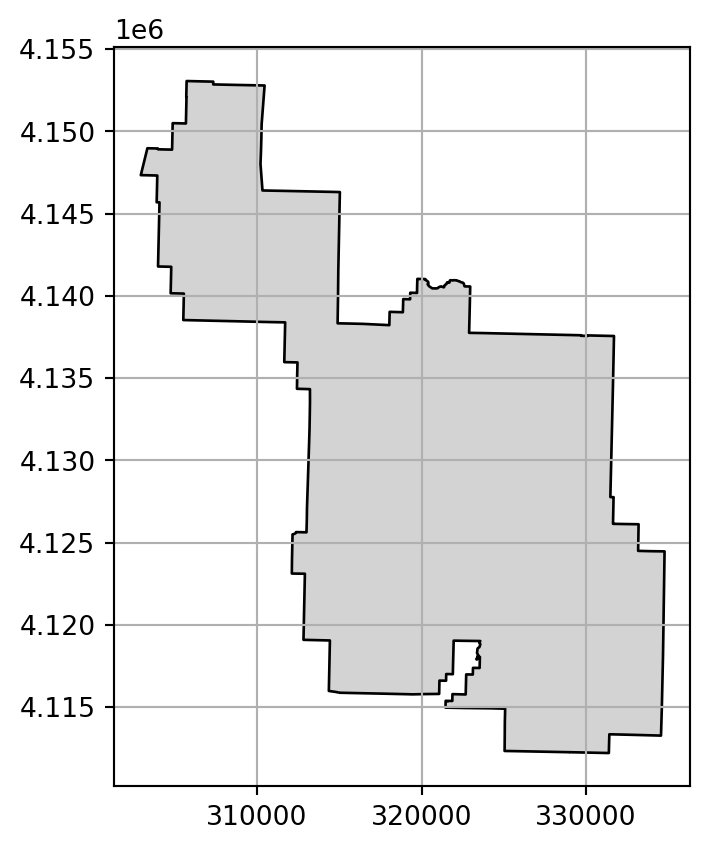
\includegraphics{01-spatial-data_files/figure-pdf/fig-zion-crs-output-2.pdf}

}

\subcaption{\label{fig-zion-crs-2}Projected (NAD83 / UTM zone 12N)}

\end{minipage}%

\caption{\label{fig-zion-crs}Examples of Coordinate Reference Systems
(CRS) for a vector layer}

\end{figure}%

We are going to elaborate on reprojection from one CRS to another
(\texttt{.to\_crs} in the above code section) in
Chapter~\ref{sec-reproj-geo-data}.

\section{Units}\label{units}

An important feature of CRSs is that they contain information about
spatial units. Clearly, it is vital to know whether a house's
measurements are in feet or meters, and the same applies to maps. It is
a good cartographic practice to add a scale bar or some other distance
indicator onto maps to demonstrate the relationship between distances on
the page or screen and distances on the ground. Likewise, it is
important for the user to be aware of the units in which the geometry
coordinates are, to ensure that subsequent calculations are done in the
right context.

Python spatial data structures in \textbf{geopandas} and
\textbf{rasterio} do not natively support the concept of measurement
units. The coordinates of a vector layer or a raster are plain numbers,
referring to an arbitrary plane. For example, according to the
\texttt{.transform} matrix of \texttt{srtm.tif} we can see that the
raster resolution is \texttt{0.000833} and that its CRS is WGS84 (EPSG:
\texttt{4326}):

\begin{Shaded}
\begin{Highlighting}[]
\NormalTok{src.meta}
\end{Highlighting}
\end{Shaded}

\begin{verbatim}
{'driver': 'GTiff',
 'dtype': 'uint16',
 'nodata': 65535.0,
 'width': 465,
 'height': 457,
 'count': 1,
 'crs': CRS.from_epsg(4326),
 'transform': Affine(0.0008333333332777796, 0.0, -113.23958321278403,
        0.0, -0.0008333333332777843, 37.512916763165805)}
\end{verbatim}

You may already know that the units of the WGS84 coordinate system
(EPSG:4326) are decimal degrees. However, that information is not
accounted for in any numeric calculation, meaning that operations such
as buffers can be returned in units of degrees, which is not appropriate
in most cases.

Consequently, you should always be aware of the CRS of your datasets and
the units they use. Typically, these are decimal degrees, in a
geographic CRS, or \(m\), in a projected CRS, although there are
exceptions. Geometric calculations such as length, area, or distance,
return plain numbers in the same units of the CRS (such as \(m\) or
\(m^2\)). It is up to the user to determine which units the result is
given in, and treat the result accordingly. For example, if the area
output was in \(m^2\) and we need the result in \(km^2\), then we need
to divide the result by \(1000^2\).

\bookmarksetup{startatroot}

\chapter{Attribute data operations}\label{sec-attr}

\section*{Prerequisites}\label{prerequisites-1}
\addcontentsline{toc}{section}{Prerequisites}

\markright{Prerequisites}

This chapter requires importing the following packages:

\begin{Shaded}
\begin{Highlighting}[]
\ImportTok{import}\NormalTok{ numpy }\ImportTok{as}\NormalTok{ np}
\ImportTok{import}\NormalTok{ matplotlib.pyplot }\ImportTok{as}\NormalTok{ plt}
\ImportTok{import}\NormalTok{ pandas }\ImportTok{as}\NormalTok{ pd}
\ImportTok{import}\NormalTok{ geopandas }\ImportTok{as}\NormalTok{ gpd}
\ImportTok{import}\NormalTok{ rasterio}
\end{Highlighting}
\end{Shaded}

It also relies on the following data files:

\begin{Shaded}
\begin{Highlighting}[]
\NormalTok{world }\OperatorTok{=}\NormalTok{ gpd.read\_file(}\StringTok{\textquotesingle{}data/world.gpkg\textquotesingle{}}\NormalTok{)}
\NormalTok{src\_elev }\OperatorTok{=}\NormalTok{ rasterio.}\BuiltInTok{open}\NormalTok{(}\StringTok{\textquotesingle{}output/elev.tif\textquotesingle{}}\NormalTok{)}
\NormalTok{src\_grain }\OperatorTok{=}\NormalTok{ rasterio.}\BuiltInTok{open}\NormalTok{(}\StringTok{\textquotesingle{}output/grain.tif\textquotesingle{}}\NormalTok{)}
\NormalTok{src\_multi\_rast }\OperatorTok{=}\NormalTok{ rasterio.}\BuiltInTok{open}\NormalTok{(}\StringTok{\textquotesingle{}data/landsat.tif\textquotesingle{}}\NormalTok{)}
\end{Highlighting}
\end{Shaded}

\section{Introduction}\label{introduction-1}

Attribute data is non-spatial information associated with geographic
(geometry) data. A bus stop provides a simple example: its position
would typically be represented by latitude and longitude coordinates
(geometry data), in addition to its name. A bus stop in London, for
example, has coordinates of \texttt{-0.098} degrees longitude and
\texttt{51.495} degrees latitude which can be represented as
\texttt{POINT\ (-0.098\ 51.495)} using the Simple Feature representation
described in Chapter~\ref{sec-spatial-class}. Attributes, such as the
name of the bus stop, are the topic of this chapter.

Another example of an attribute is the elevation value for a specific
grid cell in raster data. Unlike the vector data model, the raster data
model stores the coordinate of the grid cell indirectly, meaning the
distinction between attribute and spatial information is less clear.
Think of a pixel in the 3\textsuperscript{rd} row and the
4\textsuperscript{th} column of a raster matrix: its spatial location is
defined by its index in the matrix. In this case, we need to move four
cells in the x direction (typically east/right on maps) and three cells
in the y direction (typically south/down) from the origin. The raster's
resolution is also important as it defines the distance for each x- and
y-step. The resolution and the origin are stored in the raster's
metadata (header), which is a vital component of raster datasets which
specifies how pixels relate to geographic coordinates (see also
Chapter~\ref{sec-spatial-operations}).

This chapter teaches how to manipulate geographic objects based on
attributes such as the names of bus stops in a vector dataset and
elevations of pixels in a raster dataset. For vector data, this means
techniques such as subsetting and aggregation (see
Section~\ref{sec-vector-attribute-subsetting} and
Section~\ref{sec-vector-attribute-aggregation}). Moreover,
Section~\ref{sec-vector-attribute-joining} and
Section~\ref{sec-creating-attributes-and-removing-spatial-information}
demonstrate how to join data onto simple feature objects using a shared
ID and how to create new variables, respectively. Each of these
operations has a spatial equivalent: \texttt{{[}} operator for
subsetting a \texttt{(Geo)DataFrame} using a boolean \texttt{Series},
for example, is applicable both for subsetting objects based on their
attribute and spatial relations derived using methods such as
\texttt{.intersects}; you can also join attributes in two geographic
datasets using spatial joins. This is good news: skills developed in
this chapter are cross-transferable.
Chapter~\ref{sec-spatial-operations} extends the methods presented here
to the spatial world.

After a deep dive into various types of vector attribute operations in
the next section, raster attribute data operations are covered in
Section~\ref{sec-raster-subsetting}, which demonstrates extracting cell
values from one or more layers (raster subsetting).
Section~\ref{sec-summarizing-raster-objects} provides an overview of
`global' raster operations which can be used to summarize entire raster
datasets.

\section{Vector attribute
manipulation}\label{sec-vector-attribute-manipulation}

As mentioned in Section~\ref{sec-vector-layers}, vector layers
(\texttt{GeoDataFrame}, from package \textbf{geopandas}) are basically
extended tables (\texttt{DataFrame} from package \textbf{pandas}), the
only differences being the geometry column and class. Therefore, all
ordinary table-related operations from package \textbf{pandas} are
supported for \textbf{geopandas} vector layers as well, as shown below.

\subsection{Vector attribute
subsetting}\label{sec-vector-attribute-subsetting}

\textbf{pandas} supports several subsetting interfaces, though the most
recommended ones are \texttt{.loc}, which uses \textbf{pandas} indices,
and \texttt{.iloc}, which uses (implicit) \textbf{numpy}-style numeric
indices.

In both cases, the method is followed by square brackets, and two
indices, separated by a comma. Each index can be:

\begin{itemize}
\tightlist
\item
  A specific value, as in \texttt{1}
\item
  A \texttt{list}, as in \texttt{{[}0,2,4{]}}
\item
  A slice, as in \texttt{0:3}
\item
  \texttt{:}---indicating `all' indices, as in \texttt{{[}:{]}}
\end{itemize}

An exception to this guideline is selecting columns using a list, which
we do using shorter notation, as in
\texttt{df{[}{[}\textquotesingle{}a\textquotesingle{},\textquotesingle{}b\textquotesingle{}{]}{]}},
instead of
\texttt{df.loc{[}:,\ {[}\textquotesingle{}a\textquotesingle{},\textquotesingle{}b\textquotesingle{}{]}{]}},
to select columns \texttt{\textquotesingle{}a\textquotesingle{}} and
\texttt{\textquotesingle{}b\textquotesingle{}} from \texttt{df}.

Here are few examples of subsetting the \texttt{GeoDataFrame} of world
countries (Figure~\ref{fig-gdf-plot}). First, we are subsetting rows by
position. In the first example, we are using \texttt{{[}0:3,:{]}},
meaning `rows 1,2,3, all columns'. Keep in mind that indices in Python
start from 0, and slices are inclusive of the start and exclusive of the
end; therefore, \texttt{0:3} means indices \texttt{0}, \texttt{1},
\texttt{2}, i.e., first three rows in this example.

\begin{Shaded}
\begin{Highlighting}[]
\NormalTok{world.iloc[}\DecValTok{0}\NormalTok{:}\DecValTok{3}\NormalTok{, :]}
\end{Highlighting}
\end{Shaded}

\begin{longtable}[]{@{}llllll@{}}
\toprule\noalign{}
& iso\_a2 & name\_long & ... & gdpPercap & geometry \\
\midrule\noalign{}
\endhead
\bottomrule\noalign{}
\endlastfoot
0 & FJ & Fiji & ... & 8222.253784 & MULTIPOLYGON (((-180
-16.55522,... \\
1 & TZ & Tanzania & ... & 2402.099404 & MULTIPOLYGON (((33.90371
-0.95,... \\
2 & EH & Western Sahara & ... & NaN & MULTIPOLYGON (((-8.66559
27.656... \\
\end{longtable}

Subsetting columns by position requires specifying that we want to keep
all of the rows (\texttt{:}) and then the indexes of the columns we want
to keep.

\begin{Shaded}
\begin{Highlighting}[]
\NormalTok{world.iloc[:, }\DecValTok{0}\NormalTok{:}\DecValTok{3}\NormalTok{]}
\end{Highlighting}
\end{Shaded}

\begin{longtable}[]{@{}llll@{}}
\toprule\noalign{}
& iso\_a2 & name\_long & continent \\
\midrule\noalign{}
\endhead
\bottomrule\noalign{}
\endlastfoot
0 & FJ & Fiji & Oceania \\
1 & TZ & Tanzania & Africa \\
2 & EH & Western Sahara & Africa \\
... & ... & ... & ... \\
174 & XK & Kosovo & Europe \\
175 & TT & Trinidad and Tobago & North America \\
176 & SS & South Sudan & Africa \\
\end{longtable}

To subset rows and columns by position we need to specify both row and
column indices, separated by a comma.

\begin{Shaded}
\begin{Highlighting}[]
\NormalTok{world.iloc[}\DecValTok{0}\NormalTok{:}\DecValTok{3}\NormalTok{, }\DecValTok{0}\NormalTok{:}\DecValTok{3}\NormalTok{]}
\end{Highlighting}
\end{Shaded}

\begin{longtable}[]{@{}llll@{}}
\toprule\noalign{}
& iso\_a2 & name\_long & continent \\
\midrule\noalign{}
\endhead
\bottomrule\noalign{}
\endlastfoot
0 & FJ & Fiji & Oceania \\
1 & TZ & Tanzania & Africa \\
2 & EH & Western Sahara & Africa \\
\end{longtable}

Subsetting columns by name is not done with the \texttt{.iloc} method,
but instead requires specifying the column names in \texttt{.loc}, or
directly in a double square bracket \texttt{{[}{[}} notation.

\begin{Shaded}
\begin{Highlighting}[]
\NormalTok{world[[}\StringTok{\textquotesingle{}name\_long\textquotesingle{}}\NormalTok{, }\StringTok{\textquotesingle{}geometry\textquotesingle{}}\NormalTok{]]}
\end{Highlighting}
\end{Shaded}

\begin{longtable}[]{@{}lll@{}}
\toprule\noalign{}
& name\_long & geometry \\
\midrule\noalign{}
\endhead
\bottomrule\noalign{}
\endlastfoot
0 & Fiji & MULTIPOLYGON (((-180 -16.55522,... \\
1 & Tanzania & MULTIPOLYGON (((33.90371 -0.95,... \\
2 & Western Sahara & MULTIPOLYGON (((-8.66559 27.656... \\
... & ... & ... \\
174 & Kosovo & MULTIPOLYGON (((20.59025 41.855... \\
175 & Trinidad and Tobago & MULTIPOLYGON (((-61.68 10.76, -... \\
176 & South Sudan & MULTIPOLYGON (((30.83385 3.5091... \\
\end{longtable}

To select many successive columns, we can use the \texttt{:} (slice)
notation, as in
\texttt{world.loc{[}:,\ \textquotesingle{}name\_long\textquotesingle{}:\textquotesingle{}pop\textquotesingle{}{]}},
which selects all columns from \texttt{name\_long} to \texttt{pop}
(inclusive).

\begin{Shaded}
\begin{Highlighting}[]
\NormalTok{world.loc[:, }\StringTok{\textquotesingle{}name\_long\textquotesingle{}}\NormalTok{:}\StringTok{\textquotesingle{}pop\textquotesingle{}}\NormalTok{]}
\end{Highlighting}
\end{Shaded}

\begin{longtable}[]{@{}llllll@{}}
\toprule\noalign{}
& name\_long & continent & ... & area\_km2 & pop \\
\midrule\noalign{}
\endhead
\bottomrule\noalign{}
\endlastfoot
0 & Fiji & Oceania & ... & 19289.970733 & 885806.0 \\
1 & Tanzania & Africa & ... & 932745.792357 & 52234869.0 \\
2 & Western Sahara & Africa & ... & 96270.601041 & NaN \\
... & ... & ... & ... & ... & ... \\
174 & Kosovo & Europe & ... & 11230.261672 & 1821800.0 \\
175 & Trinidad and Tobago & North America & ... & 7737.809855 &
1354493.0 \\
176 & South Sudan & Africa & ... & 624909.099086 & 11530971.0 \\
\end{longtable}

Removing rows or columns is done using the \texttt{.drop} method. We can
remove specific rows by specifying their ids, e.g., dropping rows 2, 3,
and 5 in the following example.

\begin{Shaded}
\begin{Highlighting}[]
\NormalTok{world.drop([}\DecValTok{2}\NormalTok{, }\DecValTok{3}\NormalTok{, }\DecValTok{5}\NormalTok{])}
\end{Highlighting}
\end{Shaded}

\begin{longtable}[]{@{}llllll@{}}
\toprule\noalign{}
& iso\_a2 & name\_long & ... & gdpPercap & geometry \\
\midrule\noalign{}
\endhead
\bottomrule\noalign{}
\endlastfoot
0 & FJ & Fiji & ... & 8222.253784 & MULTIPOLYGON (((-180
-16.55522,... \\
1 & TZ & Tanzania & ... & 2402.099404 & MULTIPOLYGON (((33.90371
-0.95,... \\
4 & US & United States & ... & 51921.984639 & MULTIPOLYGON (((-171.73166
63.7... \\
... & ... & ... & ... & ... & ... \\
174 & XK & Kosovo & ... & 8698.291559 & MULTIPOLYGON (((20.59025
41.855... \\
175 & TT & Trinidad and Tobago & ... & 31181.821196 & MULTIPOLYGON
(((-61.68 10.76, -... \\
176 & SS & South Sudan & ... & 1935.879400 & MULTIPOLYGON (((30.83385
3.5091... \\
\end{longtable}

To remove specific columns we need to add an extra argument,
\texttt{axis=1} (i.e., columns).

\begin{Shaded}
\begin{Highlighting}[]
\NormalTok{world.drop([}\StringTok{\textquotesingle{}name\_long\textquotesingle{}}\NormalTok{, }\StringTok{\textquotesingle{}continent\textquotesingle{}}\NormalTok{], axis}\OperatorTok{=}\DecValTok{1}\NormalTok{)}
\end{Highlighting}
\end{Shaded}

\begin{longtable}[]{@{}llllll@{}}
\toprule\noalign{}
& iso\_a2 & region\_un & ... & gdpPercap & geometry \\
\midrule\noalign{}
\endhead
\bottomrule\noalign{}
\endlastfoot
0 & FJ & Oceania & ... & 8222.253784 & MULTIPOLYGON (((-180
-16.55522,... \\
1 & TZ & Africa & ... & 2402.099404 & MULTIPOLYGON (((33.90371
-0.95,... \\
2 & EH & Africa & ... & NaN & MULTIPOLYGON (((-8.66559 27.656... \\
... & ... & ... & ... & ... & ... \\
174 & XK & Europe & ... & 8698.291559 & MULTIPOLYGON (((20.59025
41.855... \\
175 & TT & Americas & ... & 31181.821196 & MULTIPOLYGON (((-61.68 10.76,
-... \\
176 & SS & Africa & ... & 1935.879400 & MULTIPOLYGON (((30.83385
3.5091... \\
\end{longtable}

We can also rename columns using the \texttt{.rename} method, in which
we pass a dictionary with items of the form \texttt{old\_name:new\_name}
to the \texttt{columns} argument.

\begin{Shaded}
\begin{Highlighting}[]
\NormalTok{world[[}\StringTok{\textquotesingle{}name\_long\textquotesingle{}}\NormalTok{, }\StringTok{\textquotesingle{}pop\textquotesingle{}}\NormalTok{]].rename(columns}\OperatorTok{=}\NormalTok{\{}\StringTok{\textquotesingle{}pop\textquotesingle{}}\NormalTok{: }\StringTok{\textquotesingle{}population\textquotesingle{}}\NormalTok{\})}
\end{Highlighting}
\end{Shaded}

\begin{longtable}[]{@{}lll@{}}
\toprule\noalign{}
& name\_long & population \\
\midrule\noalign{}
\endhead
\bottomrule\noalign{}
\endlastfoot
0 & Fiji & 885806.0 \\
1 & Tanzania & 52234869.0 \\
2 & Western Sahara & NaN \\
... & ... & ... \\
174 & Kosovo & 1821800.0 \\
175 & Trinidad and Tobago & 1354493.0 \\
176 & South Sudan & 11530971.0 \\
\end{longtable}

The standard \textbf{numpy} comparison operators
(Table~\ref{tbl-comparison-operators}) can be used in boolean subsetting
with \textbf{pandas}/\textbf{geopandas}.

\begin{longtable}[]{@{}cc@{}}
\caption{Comparison operators that return boolean values
(\texttt{True}/\texttt{False}).}\label{tbl-comparison-operators}\tabularnewline
\toprule\noalign{}
\texttt{Symbol} & \texttt{Name} \\
\midrule\noalign{}
\endfirsthead
\toprule\noalign{}
\texttt{Symbol} & \texttt{Name} \\
\midrule\noalign{}
\endhead
\bottomrule\noalign{}
\endlastfoot
\texttt{==} & Equal to \\
\texttt{!=} & Not equal to \\
\texttt{\textgreater{}}, \texttt{\textless{}} & Greater/Less than \\
\texttt{\textgreater{}=}, \texttt{\textless{}=} & Greater/Less than or
equal \\
\texttt{\&}, \texttt{\textbar{}}, \texttt{\textasciitilde{}} & Logical
operators: And, Or, Not \\
\end{longtable}

The following example demonstrates logical vectors for subsetting by
creating a new \texttt{GeoDataFrame} object called
\texttt{small\_countries} that contains only those countries and other
territories from the \texttt{world} object whose surface area is smaller
than 10,000 \(km^2\). The first step is to create a logical vector (a
\texttt{Series} object) that is \texttt{True} for countries with an area
smaller than 10,000 \(km^2\) and \texttt{False} otherwise. Then, we use
this vector to subset the \texttt{world} dataset, which returns a new
\texttt{GeoDataFrame} object containing only the small countries.

\begin{Shaded}
\begin{Highlighting}[]
\NormalTok{idx\_small }\OperatorTok{=}\NormalTok{ world[}\StringTok{\textquotesingle{}area\_km2\textquotesingle{}}\NormalTok{] }\OperatorTok{\textless{}} \DecValTok{10000}  \CommentTok{\#\# a logical \textquotesingle{}Series\textquotesingle{}}
\NormalTok{small\_countries }\OperatorTok{=}\NormalTok{ world[idx\_small]}
\NormalTok{small\_countries}
\end{Highlighting}
\end{Shaded}

\begin{longtable}[]{@{}llllll@{}}
\toprule\noalign{}
& iso\_a2 & name\_long & ... & gdpPercap & geometry \\
\midrule\noalign{}
\endhead
\bottomrule\noalign{}
\endlastfoot
45 & PR & Puerto Rico & ... & 35066.046376 & MULTIPOLYGON (((-66.28243
18.51... \\
79 & PS & Palestine & ... & 4319.528283 & MULTIPOLYGON (((35.39756
31.489... \\
89 & VU & Vanuatu & ... & 2892.341604 & MULTIPOLYGON (((166.79316
-15.6... \\
... & ... & ... & ... & ... & ... \\
160 & None & Northern Cyprus & ... & NaN & MULTIPOLYGON (((32.73178
35.140... \\
161 & CY & Cyprus & ... & 29786.365653 & MULTIPOLYGON (((32.73178
35.140... \\
175 & TT & Trinidad and Tobago & ... & 31181.821196 & MULTIPOLYGON
(((-61.68 10.76, -... \\
\end{longtable}

A more concise command, which omits the intermediary object by combining
the two steps into one, generates the same result.

\begin{Shaded}
\begin{Highlighting}[]
\NormalTok{small\_countries }\OperatorTok{=}\NormalTok{ world[world[}\StringTok{\textquotesingle{}area\_km2\textquotesingle{}}\NormalTok{] }\OperatorTok{\textless{}} \DecValTok{10000}\NormalTok{]}
\NormalTok{small\_countries}
\end{Highlighting}
\end{Shaded}

\begin{longtable}[]{@{}llllll@{}}
\toprule\noalign{}
& iso\_a2 & name\_long & ... & gdpPercap & geometry \\
\midrule\noalign{}
\endhead
\bottomrule\noalign{}
\endlastfoot
45 & PR & Puerto Rico & ... & 35066.046376 & MULTIPOLYGON (((-66.28243
18.51... \\
79 & PS & Palestine & ... & 4319.528283 & MULTIPOLYGON (((35.39756
31.489... \\
89 & VU & Vanuatu & ... & 2892.341604 & MULTIPOLYGON (((166.79316
-15.6... \\
... & ... & ... & ... & ... & ... \\
160 & None & Northern Cyprus & ... & NaN & MULTIPOLYGON (((32.73178
35.140... \\
161 & CY & Cyprus & ... & 29786.365653 & MULTIPOLYGON (((32.73178
35.140... \\
175 & TT & Trinidad and Tobago & ... & 31181.821196 & MULTIPOLYGON
(((-61.68 10.76, -... \\
\end{longtable}

We can also combine indexes using logical operators, such as \texttt{\&}
(and), \texttt{\textbar{}} (or), and \texttt{\textasciitilde{}} (not).

\begin{Shaded}
\begin{Highlighting}[]
\NormalTok{idx\_small }\OperatorTok{=}\NormalTok{ world[}\StringTok{\textquotesingle{}area\_km2\textquotesingle{}}\NormalTok{] }\OperatorTok{\textless{}} \DecValTok{10000}
\NormalTok{idx\_asia }\OperatorTok{=}\NormalTok{ world[}\StringTok{\textquotesingle{}continent\textquotesingle{}}\NormalTok{] }\OperatorTok{==} \StringTok{\textquotesingle{}Asia\textquotesingle{}}
\NormalTok{world.loc[idx\_small }\OperatorTok{\&}\NormalTok{ idx\_asia, [}\StringTok{\textquotesingle{}name\_long\textquotesingle{}}\NormalTok{, }\StringTok{\textquotesingle{}continent\textquotesingle{}}\NormalTok{, }\StringTok{\textquotesingle{}area\_km2\textquotesingle{}}\NormalTok{]]}
\end{Highlighting}
\end{Shaded}

\begin{longtable}[]{@{}llll@{}}
\toprule\noalign{}
& name\_long & continent & area\_km2 \\
\midrule\noalign{}
\endhead
\bottomrule\noalign{}
\endlastfoot
79 & Palestine & Asia & 5037.103826 \\
160 & Northern Cyprus & Asia & 3786.364506 \\
161 & Cyprus & Asia & 6207.006191 \\
\end{longtable}

The various methods shown above can be chained for any combination with
several subsetting steps. For example, the following code selects only
countries from Asia, keeps only the \texttt{name\_long} and
\texttt{continent} columns, and then selects the first five rows.

\begin{Shaded}
\begin{Highlighting}[]
\NormalTok{world[world[}\StringTok{\textquotesingle{}continent\textquotesingle{}}\NormalTok{] }\OperatorTok{==} \StringTok{\textquotesingle{}Asia\textquotesingle{}}\NormalTok{]  }\OperatorTok{\textbackslash{}}
\NormalTok{    .loc[:, [}\StringTok{\textquotesingle{}name\_long\textquotesingle{}}\NormalTok{, }\StringTok{\textquotesingle{}continent\textquotesingle{}}\NormalTok{]]  }\OperatorTok{\textbackslash{}}
\NormalTok{    .iloc[}\DecValTok{0}\NormalTok{:}\DecValTok{5}\NormalTok{, :]}
\end{Highlighting}
\end{Shaded}

\begin{longtable}[]{@{}lll@{}}
\toprule\noalign{}
& name\_long & continent \\
\midrule\noalign{}
\endhead
\bottomrule\noalign{}
\endlastfoot
5 & Kazakhstan & Asia \\
6 & Uzbekistan & Asia \\
8 & Indonesia & Asia \\
24 & Timor-Leste & Asia \\
76 & Israel & Asia \\
\end{longtable}

Logical operators \texttt{\&}, \texttt{\textbar{}}, and
\texttt{\textasciitilde{}} (Table~\ref{tbl-comparison-operators}) can be
used to combine multiple conditions. For example, here are all countries
in North America or South America. Keep in mind that the parentheses
around each condition (here, and in analogous cases using other
operators) are crucial; otherwise, due to Python's precedence
rules\footnote{\url{https://docs.python.org/3/reference/expressions.html\#operator-precedence}},
the \texttt{\textbar{}} operator is executed before \texttt{==} and we
get an error.

\begin{Shaded}
\begin{Highlighting}[]
\NormalTok{world[}
\NormalTok{        (world[}\StringTok{\textquotesingle{}continent\textquotesingle{}}\NormalTok{] }\OperatorTok{==} \StringTok{\textquotesingle{}North America\textquotesingle{}}\NormalTok{) }\OperatorTok{|} 
\NormalTok{        (world[}\StringTok{\textquotesingle{}continent\textquotesingle{}}\NormalTok{] }\OperatorTok{==}  \StringTok{\textquotesingle{}South America\textquotesingle{}}\NormalTok{)}
\NormalTok{    ]  }\OperatorTok{\textbackslash{}}
\NormalTok{    .loc[:, [}\StringTok{\textquotesingle{}name\_long\textquotesingle{}}\NormalTok{, }\StringTok{\textquotesingle{}continent\textquotesingle{}}\NormalTok{]]}
\end{Highlighting}
\end{Shaded}

\begin{longtable}[]{@{}lll@{}}
\toprule\noalign{}
& name\_long & continent \\
\midrule\noalign{}
\endhead
\bottomrule\noalign{}
\endlastfoot
3 & Canada & North America \\
4 & United States & North America \\
9 & Argentina & South America \\
... & ... & ... \\
47 & Cuba & North America \\
156 & Paraguay & South America \\
175 & Trinidad and Tobago & North America \\
\end{longtable}

However, specifically, expressions combining multiple comparisons with
\texttt{==} combined with \texttt{\textbar{}} can be replaced with the
\texttt{.isin} method and a \texttt{list} of values to compare with. The
advantage of \texttt{.isin} is more concise and easy to manage code,
especially when the number of comparisons is large. For example, the
following expression gives the same result as above.

\begin{Shaded}
\begin{Highlighting}[]
\NormalTok{world[world[}\StringTok{\textquotesingle{}continent\textquotesingle{}}\NormalTok{].isin([}\StringTok{\textquotesingle{}North America\textquotesingle{}}\NormalTok{, }\StringTok{\textquotesingle{}South America\textquotesingle{}}\NormalTok{])]  }\OperatorTok{\textbackslash{}}
\NormalTok{    .loc[:, [}\StringTok{\textquotesingle{}name\_long\textquotesingle{}}\NormalTok{, }\StringTok{\textquotesingle{}continent\textquotesingle{}}\NormalTok{]]}
\end{Highlighting}
\end{Shaded}

\begin{longtable}[]{@{}lll@{}}
\toprule\noalign{}
& name\_long & continent \\
\midrule\noalign{}
\endhead
\bottomrule\noalign{}
\endlastfoot
3 & Canada & North America \\
4 & United States & North America \\
9 & Argentina & South America \\
... & ... & ... \\
47 & Cuba & North America \\
156 & Paraguay & South America \\
175 & Trinidad and Tobago & North America \\
\end{longtable}

\subsection{Vector attribute
aggregation}\label{sec-vector-attribute-aggregation}

Aggregation involves summarizing data based on one or more
\emph{grouping variables} (typically values in a column; geographic
aggregation is covered in Section~\ref{sec-vector-spatial-aggregation}).
A classic example of this attribute-based aggregation is calculating the
number of people per continent based on country-level data (one row per
country). The \texttt{world} dataset contains the necessary ingredients:
the columns \texttt{pop} and \texttt{continent}, the target variable and
the grouping variable, respectively. The aim is to find the
\texttt{sum()} of country populations for each continent, resulting in a
smaller table or vector layer (of continents). Since aggregation is a
form of data reduction, it can be a useful early step when working with
large datasets.

Attribute-based aggregation can be achieved using a combination of
\texttt{.groupby} and \texttt{.sum} (package \textbf{pandas}), where the
former groups the data by the grouping variable(s) and the latter
calculates the sum of the specified column(s). The
\texttt{.reset\_index} method moves the grouping variable into an
ordinary column, rather than an index (the default), which is something
we typically want to do.

\begin{Shaded}
\begin{Highlighting}[]
\NormalTok{world\_agg1 }\OperatorTok{=}\NormalTok{ world.groupby(}\StringTok{\textquotesingle{}continent\textquotesingle{}}\NormalTok{)[[}\StringTok{\textquotesingle{}pop\textquotesingle{}}\NormalTok{]].}\BuiltInTok{sum}\NormalTok{().reset\_index()}
\NormalTok{world\_agg1}
\end{Highlighting}
\end{Shaded}

\begin{longtable}[]{@{}lll@{}}
\toprule\noalign{}
& continent & pop \\
\midrule\noalign{}
\endhead
\bottomrule\noalign{}
\endlastfoot
0 & Africa & 1.154947e+09 \\
1 & Antarctica & 0.000000e+00 \\
2 & Asia & 4.311408e+09 \\
... & ... & ... \\
5 & Oceania & 3.775783e+07 \\
6 & Seven seas (open ocean) & 0.000000e+00 \\
7 & South America & 4.120608e+08 \\
\end{longtable}

The result, in this case, is a (non-spatial) table with eight rows, one
per unique value in \texttt{continent}, and two columns reporting the
name and population of each continent.

If we want to include the geometry in the aggregation result, we can use
the \texttt{.dissolve} method. That way, in addition to the summed
population, we also get the associated geometry per continent, i.e., the
union of all countries. Note that we use the \texttt{by} parameter to
choose which column(s) are used for grouping, and the \texttt{aggfunc}
parameter to choose the aggregation function for non-geometry columns.
Again, note that the \texttt{.reset\_index} method is used (here, and
elsewhere in the book) to turn \textbf{pandas} and \textbf{geopandas}
row \emph{indices}, which are automatically created for grouping
variables in grouping operations such as \texttt{.dissolve}, `back' into
ordinary columns, which are more appropriate in the scope of this book.

\begin{Shaded}
\begin{Highlighting}[]
\NormalTok{world\_agg2 }\OperatorTok{=}\NormalTok{ world[[}\StringTok{\textquotesingle{}continent\textquotesingle{}}\NormalTok{, }\StringTok{\textquotesingle{}pop\textquotesingle{}}\NormalTok{, }\StringTok{\textquotesingle{}geometry\textquotesingle{}}\NormalTok{]] }\OperatorTok{\textbackslash{}}
\NormalTok{    .dissolve(by}\OperatorTok{=}\StringTok{\textquotesingle{}continent\textquotesingle{}}\NormalTok{, aggfunc}\OperatorTok{=}\StringTok{\textquotesingle{}sum\textquotesingle{}}\NormalTok{) }\OperatorTok{\textbackslash{}}
\NormalTok{    .reset\_index()}
\NormalTok{world\_agg2}
\end{Highlighting}
\end{Shaded}

\begin{longtable}[]{@{}llll@{}}
\toprule\noalign{}
& continent & geometry & pop \\
\midrule\noalign{}
\endhead
\bottomrule\noalign{}
\endlastfoot
0 & Africa & MULTIPOLYGON (((-11.43878 6.785... & 1.154947e+09 \\
1 & Antarctica & MULTIPOLYGON (((-61.13898 -79.9... & 0.000000e+00 \\
2 & Asia & MULTIPOLYGON (((48.67923 14.003... & 4.311408e+09 \\
... & ... & ... & ... \\
5 & Oceania & MULTIPOLYGON (((147.91405 -43.2... & 3.775783e+07 \\
6 & Seven seas (open ocean) & POLYGON ((68.935 -48.625, 68.86... &
0.000000e+00 \\
7 & South America & MULTIPOLYGON (((-68.63999 -55.5... & 4.120608e+08 \\
\end{longtable}

In this case, the resulting \texttt{world\_agg2} object is a
\texttt{GeoDataFrame} containing 8 features representing the continents
of the world that we can plot (Figure~\ref{fig-spatial-aggregation}).
The \texttt{plt.subplots} function is hereby used to control plot
dimensions (to make the plot wider and narrower) (see
Section~\ref{sec-static-styling}).

\begin{Shaded}
\begin{Highlighting}[]
\NormalTok{fig, ax }\OperatorTok{=}\NormalTok{ plt.subplots(figsize}\OperatorTok{=}\NormalTok{(}\DecValTok{6}\NormalTok{, }\DecValTok{3}\NormalTok{))}
\NormalTok{world\_agg2.plot(column}\OperatorTok{=}\StringTok{\textquotesingle{}pop\textquotesingle{}}\NormalTok{, edgecolor}\OperatorTok{=}\StringTok{\textquotesingle{}black\textquotesingle{}}\NormalTok{, legend}\OperatorTok{=}\VariableTok{True}\NormalTok{, ax}\OperatorTok{=}\NormalTok{ax)}\OperatorTok{;}
\end{Highlighting}
\end{Shaded}

\begin{figure}[H]

\centering{

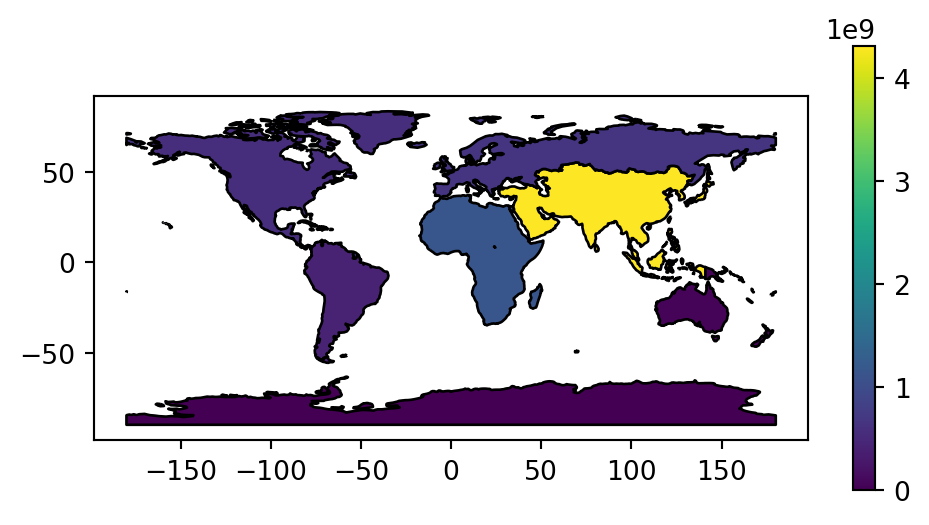
\includegraphics{02-attribute-operations_files/figure-pdf/fig-spatial-aggregation-output-1.pdf}

}

\caption{\label{fig-spatial-aggregation}Continents with summed
population}

\end{figure}%

Other options for the \texttt{aggfunc} parameter in \texttt{.dissolve}
\href{https://geopandas.org/en/stable/docs/user_guide/aggregation_with_dissolve.html}{include}
\texttt{\textquotesingle{}first\textquotesingle{}},
\texttt{\textquotesingle{}last\textquotesingle{}},
\texttt{\textquotesingle{}min\textquotesingle{}},
\texttt{\textquotesingle{}max\textquotesingle{}},
\texttt{\textquotesingle{}sum\textquotesingle{}},
\texttt{\textquotesingle{}mean\textquotesingle{}},
\texttt{\textquotesingle{}median\textquotesingle{}}. Additionally, we
can pass custom functions here.

As a more complex example, the following code shows how we can calculate
the total population, area, and count of countries, per continent. It is
done by passing a dictionary to the \texttt{aggfunc} parameter, where
the keys are the column names and the values are the aggregation
functions. The result is a \texttt{GeoDataFrame} object with 8 rows (one
per continent) and 4 columns (one for the continent name and one for
each of the three aggregated attributes). The \texttt{rename} method is
used to rename the
\texttt{\textquotesingle{}name\_long\textquotesingle{}} column into
\texttt{\textquotesingle{}n\textquotesingle{}}, as it now expresses the
count of names (i.e., the number of countries) rather than their names.

\begin{Shaded}
\begin{Highlighting}[]
\NormalTok{world\_agg3 }\OperatorTok{=}\NormalTok{ world.dissolve(}
\NormalTok{    by}\OperatorTok{=}\StringTok{\textquotesingle{}continent\textquotesingle{}}\NormalTok{, }
\NormalTok{    aggfunc}\OperatorTok{=}\NormalTok{\{}
        \StringTok{\textquotesingle{}name\_long\textquotesingle{}}\NormalTok{: }\StringTok{\textquotesingle{}count\textquotesingle{}}\NormalTok{,}
        \StringTok{\textquotesingle{}pop\textquotesingle{}}\NormalTok{: }\StringTok{\textquotesingle{}sum\textquotesingle{}}\NormalTok{,}
        \StringTok{\textquotesingle{}area\_km2\textquotesingle{}}\NormalTok{: }\StringTok{\textquotesingle{}sum\textquotesingle{}}
\NormalTok{    \}).rename(columns}\OperatorTok{=}\NormalTok{\{}\StringTok{\textquotesingle{}name\_long\textquotesingle{}}\NormalTok{: }\StringTok{\textquotesingle{}n\textquotesingle{}}\NormalTok{\}).reset\_index()}
\NormalTok{world\_agg3}
\end{Highlighting}
\end{Shaded}

\begin{longtable}[]{@{}llllll@{}}
\toprule\noalign{}
& continent & geometry & n & pop & area\_km2 \\
\midrule\noalign{}
\endhead
\bottomrule\noalign{}
\endlastfoot
0 & Africa & MULTIPOLYGON (((-11.43878 6.785... & 51 & 1.154947e+09 &
2.994620e+07 \\
1 & Antarctica & MULTIPOLYGON (((-61.13898 -79.9... & 1 & 0.000000e+00 &
1.233596e+07 \\
2 & Asia & MULTIPOLYGON (((48.67923 14.003... & 47 & 4.311408e+09 &
3.125246e+07 \\
... & ... & ... & ... & ... & ... \\
5 & Oceania & MULTIPOLYGON (((147.91405 -43.2... & 7 & 3.775783e+07 &
8.504489e+06 \\
6 & Seven seas (open ocean) & POLYGON ((68.935 -48.625, 68.86... & 1 &
0.000000e+00 & 1.160257e+04 \\
7 & South America & MULTIPOLYGON (((-68.63999 -55.5... & 13 &
4.120608e+08 & 1.776259e+07 \\
\end{longtable}

Figure~\ref{fig-spatial-aggregation-different-functions} visualizes the
three aggregated attributes of our resulting layer \texttt{world\_agg3}.

\begin{Shaded}
\begin{Highlighting}[]
\CommentTok{\# Summed population}
\NormalTok{fig, ax }\OperatorTok{=}\NormalTok{ plt.subplots(figsize}\OperatorTok{=}\NormalTok{(}\DecValTok{5}\NormalTok{, }\FloatTok{2.5}\NormalTok{))}
\NormalTok{world\_agg3.plot(column}\OperatorTok{=}\StringTok{\textquotesingle{}pop\textquotesingle{}}\NormalTok{, edgecolor}\OperatorTok{=}\StringTok{\textquotesingle{}black\textquotesingle{}}\NormalTok{, legend}\OperatorTok{=}\VariableTok{True}\NormalTok{, ax}\OperatorTok{=}\NormalTok{ax)}\OperatorTok{;}
\CommentTok{\# Summed area}
\NormalTok{fig, ax }\OperatorTok{=}\NormalTok{ plt.subplots(figsize}\OperatorTok{=}\NormalTok{(}\DecValTok{5}\NormalTok{, }\FloatTok{2.5}\NormalTok{))}
\NormalTok{world\_agg3.plot(column}\OperatorTok{=}\StringTok{\textquotesingle{}area\_km2\textquotesingle{}}\NormalTok{, edgecolor}\OperatorTok{=}\StringTok{\textquotesingle{}black\textquotesingle{}}\NormalTok{, legend}\OperatorTok{=}\VariableTok{True}\NormalTok{, ax}\OperatorTok{=}\NormalTok{ax)}\OperatorTok{;}
\CommentTok{\# Count of countries}
\NormalTok{fig, ax }\OperatorTok{=}\NormalTok{ plt.subplots(figsize}\OperatorTok{=}\NormalTok{(}\DecValTok{5}\NormalTok{, }\FloatTok{2.5}\NormalTok{))}
\NormalTok{world\_agg3.plot(column}\OperatorTok{=}\StringTok{\textquotesingle{}n\textquotesingle{}}\NormalTok{, edgecolor}\OperatorTok{=}\StringTok{\textquotesingle{}black\textquotesingle{}}\NormalTok{, legend}\OperatorTok{=}\VariableTok{True}\NormalTok{, ax}\OperatorTok{=}\NormalTok{ax)}\OperatorTok{;}
\end{Highlighting}
\end{Shaded}

\begin{figure}

\begin{minipage}{0.33\linewidth}

\centering{

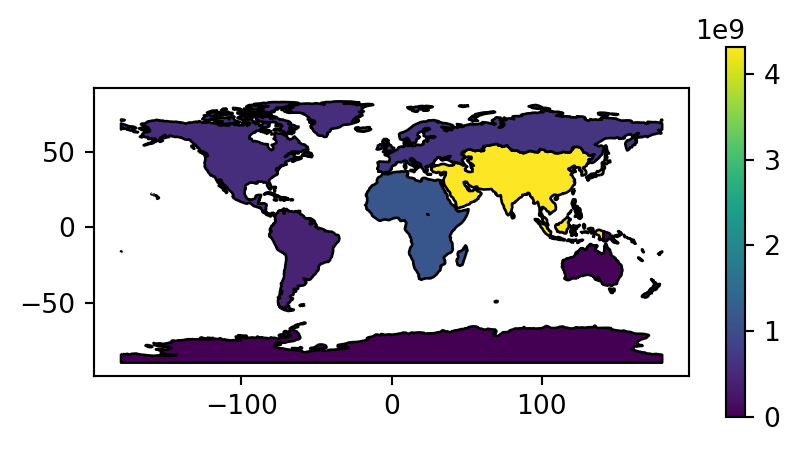
\includegraphics{02-attribute-operations_files/figure-pdf/fig-spatial-aggregation-different-functions-output-1.pdf}

}

\subcaption{\label{fig-spatial-aggregation-different-functions-1}Summed
population}

\end{minipage}%
%
\begin{minipage}{0.33\linewidth}

\centering{

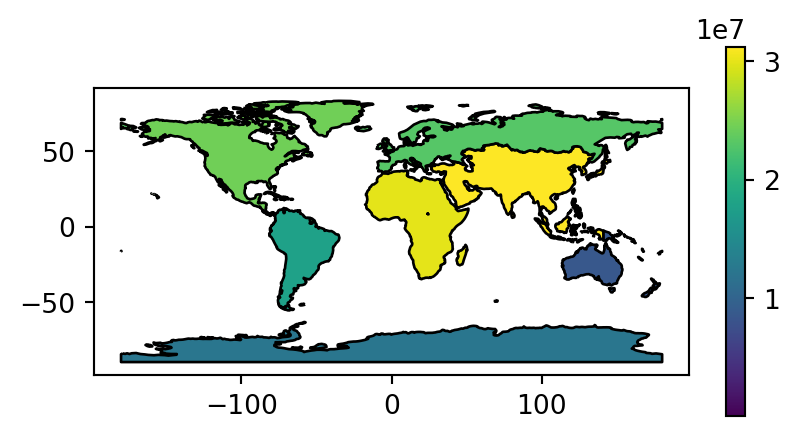
\includegraphics{02-attribute-operations_files/figure-pdf/fig-spatial-aggregation-different-functions-output-2.pdf}

}

\subcaption{\label{fig-spatial-aggregation-different-functions-2}Summed
area}

\end{minipage}%
%
\begin{minipage}{0.33\linewidth}

\centering{

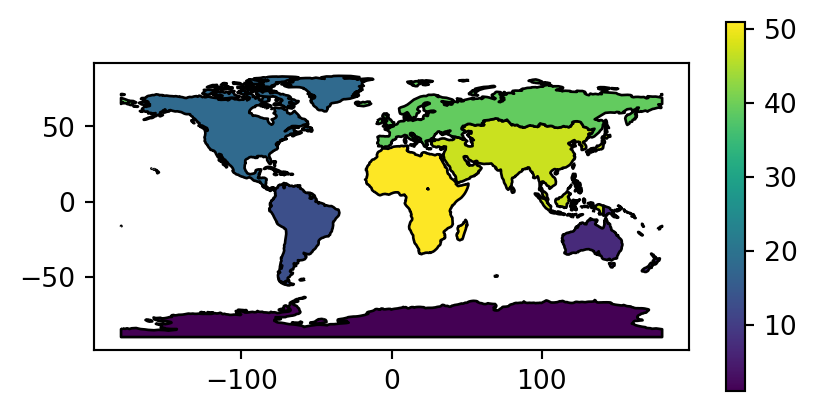
\includegraphics{02-attribute-operations_files/figure-pdf/fig-spatial-aggregation-different-functions-output-3.pdf}

}

\subcaption{\label{fig-spatial-aggregation-different-functions-3}Count
of countries}

\end{minipage}%

\caption{\label{fig-spatial-aggregation-different-functions}Continent's
properties, calculated using spatial aggregation using different
functions}

\end{figure}%

There are several other table-related operations that are possible, such
as creating new columns or sorting the values. In the following code
example, given the \texttt{world\_agg3} continent summary
(Figure~\ref{fig-spatial-aggregation-different-functions}), we:

\begin{itemize}
\tightlist
\item
  drop the geometry column,
\item
  calculate population density of each continent,
\item
  arrange continents by the number of countries each contains, and
\item
  keep only the 3 most country-rich continents.
\end{itemize}

\begin{Shaded}
\begin{Highlighting}[]
\NormalTok{world\_agg4 }\OperatorTok{=}\NormalTok{ world\_agg3.drop(columns}\OperatorTok{=}\NormalTok{[}\StringTok{\textquotesingle{}geometry\textquotesingle{}}\NormalTok{])}
\NormalTok{world\_agg4[}\StringTok{\textquotesingle{}density\textquotesingle{}}\NormalTok{] }\OperatorTok{=}\NormalTok{ world\_agg4[}\StringTok{\textquotesingle{}pop\textquotesingle{}}\NormalTok{] }\OperatorTok{/}\NormalTok{ world\_agg4[}\StringTok{\textquotesingle{}area\_km2\textquotesingle{}}\NormalTok{]}
\NormalTok{world\_agg4 }\OperatorTok{=}\NormalTok{ world\_agg4.sort\_values(by}\OperatorTok{=}\StringTok{\textquotesingle{}n\textquotesingle{}}\NormalTok{, ascending}\OperatorTok{=}\VariableTok{False}\NormalTok{)}
\NormalTok{world\_agg4 }\OperatorTok{=}\NormalTok{ world\_agg4.head(}\DecValTok{3}\NormalTok{)}
\NormalTok{world\_agg4}
\end{Highlighting}
\end{Shaded}

\begin{longtable}[]{@{}llllll@{}}
\toprule\noalign{}
& continent & n & pop & area\_km2 & density \\
\midrule\noalign{}
\endhead
\bottomrule\noalign{}
\endlastfoot
0 & Africa & 51 & 1.154947e+09 & 2.994620e+07 & 38.567388 \\
2 & Asia & 47 & 4.311408e+09 & 3.125246e+07 & 137.954201 \\
3 & Europe & 39 & 6.690363e+08 & 2.306522e+07 & 29.006283 \\
\end{longtable}

\subsection{Vector attribute
joining}\label{sec-vector-attribute-joining}

Combining data from different sources is a common task in data
preparation. Joins do this by combining tables based on a shared `key'
variable. \textbf{pandas} has a function named \texttt{pd.merge} for
joining \texttt{(Geo)DataFrames} based on common column(s) that follows
conventions used in the database language SQL (Grolemund and Wickham
2016). The \texttt{pd.merge} result can be either a \texttt{DataFrame}
or a \texttt{GeoDataFrame} object, depending on the inputs.

A common type of attribute join on spatial data is to join
\texttt{DataFrames} to \texttt{GeoDataFrames}. To achieve this, we use
\texttt{pd.merge} with a \texttt{GeoDataFrame} as the first argument and
add columns to it from a \texttt{DataFrame} specified as the second
argument. In the following example, we combine data on coffee production
with the \texttt{world} dataset. The coffee data is in a
\texttt{DataFrame} called \texttt{coffee\_data} imported from a CSV file
of major coffee-producing nations.

\begin{Shaded}
\begin{Highlighting}[]
\NormalTok{coffee\_data }\OperatorTok{=}\NormalTok{ pd.read\_csv(}\StringTok{\textquotesingle{}data/coffee\_data.csv\textquotesingle{}}\NormalTok{)}
\NormalTok{coffee\_data}
\end{Highlighting}
\end{Shaded}

\begin{longtable}[]{@{}llll@{}}
\toprule\noalign{}
& name\_long & coffee\_production\_2016 & coffee\_production\_2017 \\
\midrule\noalign{}
\endhead
\bottomrule\noalign{}
\endlastfoot
0 & Angola & NaN & NaN \\
1 & Bolivia & 3.0 & 4.0 \\
2 & Brazil & 3277.0 & 2786.0 \\
... & ... & ... & ... \\
44 & Zambia & 3.0 & NaN \\
45 & Zimbabwe & 1.0 & 1.0 \\
46 & Others & 23.0 & 26.0 \\
\end{longtable}

Its columns are \texttt{name\_long}---country name, and
\texttt{coffee\_production\_2016} and
\texttt{coffee\_production\_2017}---estimated values for coffee
production in units of 60-kg bags per year, for 2016 and 2017,
respectively.

A left join, which preserves the first dataset, merges \texttt{world}
with \texttt{coffee\_data}, based on the common
\texttt{\textquotesingle{}name\_long\textquotesingle{}} column:

\begin{Shaded}
\begin{Highlighting}[]
\NormalTok{world\_coffee }\OperatorTok{=}\NormalTok{ pd.merge(world, coffee\_data, on}\OperatorTok{=}\StringTok{\textquotesingle{}name\_long\textquotesingle{}}\NormalTok{, how}\OperatorTok{=}\StringTok{\textquotesingle{}left\textquotesingle{}}\NormalTok{)}
\NormalTok{world\_coffee}
\end{Highlighting}
\end{Shaded}

\begin{longtable}[]{@{}llllll@{}}
\toprule\noalign{}
& iso\_a2 & name\_long & ... & coffee\_production\_2016 &
coffee\_production\_2017 \\
\midrule\noalign{}
\endhead
\bottomrule\noalign{}
\endlastfoot
0 & FJ & Fiji & ... & NaN & NaN \\
1 & TZ & Tanzania & ... & 81.0 & 66.0 \\
2 & EH & Western Sahara & ... & NaN & NaN \\
... & ... & ... & ... & ... & ... \\
174 & XK & Kosovo & ... & NaN & NaN \\
175 & TT & Trinidad and Tobago & ... & NaN & NaN \\
176 & SS & South Sudan & ... & NaN & NaN \\
\end{longtable}

The result is a \texttt{GeoDataFrame} object identical to the original
\texttt{world} object, but with two new variables
(\texttt{coffee\_production\_2016} and
\texttt{coffee\_production\_2017}) on coffee production. This can be
plotted as a map, as illustrated (for \texttt{coffee\_production\_2017})
in Figure~\ref{fig-join-coffee-production}. Note that, here and in many
other examples in later chapters, we are using a technique to plot two
layers (all of the world countries outline, and coffee production with
symbology) at once, which will be `formally' introduced towards the end
of the book in Section~\ref{sec-plot-static-layers}.

\begin{Shaded}
\begin{Highlighting}[]
\NormalTok{base }\OperatorTok{=}\NormalTok{ world\_coffee.plot(color}\OperatorTok{=}\StringTok{\textquotesingle{}white\textquotesingle{}}\NormalTok{, edgecolor}\OperatorTok{=}\StringTok{\textquotesingle{}lightgrey\textquotesingle{}}\NormalTok{)}
\NormalTok{coffee\_map }\OperatorTok{=}\NormalTok{ world\_coffee.plot(ax}\OperatorTok{=}\NormalTok{base, column}\OperatorTok{=}\StringTok{\textquotesingle{}coffee\_production\_2017\textquotesingle{}}\NormalTok{)}\OperatorTok{;}
\end{Highlighting}
\end{Shaded}

\begin{figure}[H]

\centering{

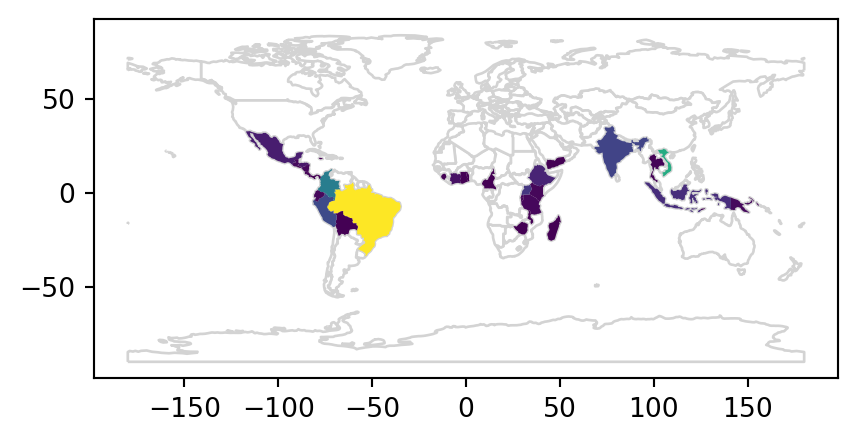
\includegraphics{02-attribute-operations_files/figure-pdf/fig-join-coffee-production-output-1.pdf}

}

\caption{\label{fig-join-coffee-production}World coffee production,
thousand 60-kg bags by country, in 2017 (source: International Coffee
Organization).}

\end{figure}%

To work, attribute-based joins need a `key variable' in both datasets
(\texttt{on} parameter of \texttt{pd.merge}). In the above example, both
\texttt{world\_coffee} and \texttt{world} DataFrames contained a column
called \texttt{name\_long}.

\begin{tcolorbox}[enhanced jigsaw, breakable, title=\textcolor{quarto-callout-note-color}{\faInfo}\hspace{0.5em}{Note}, arc=.35mm, opacitybacktitle=0.6, left=2mm, colback=white, bottomrule=.15mm, bottomtitle=1mm, toptitle=1mm, colframe=quarto-callout-note-color-frame, leftrule=.75mm, rightrule=.15mm, toprule=.15mm, titlerule=0mm, opacityback=0, colbacktitle=quarto-callout-note-color!10!white, coltitle=black]

By default, \texttt{pd.merge} uses all columns with matching names.
However, it is recommended to explicitly specify the names of the
columns to be used for matching, like we did in the last example.

\end{tcolorbox}

In case where column names are not the same, you can use
\texttt{left\_on} and \texttt{right\_on} to specify the respective
columns.

Note that the result \texttt{world\_coffee} has the same number of rows
as the original dataset \texttt{world}. Although there are only 47 rows
in \texttt{coffee\_data}, all 177 country records are kept intact in
\texttt{world\_coffee}. Rows in the original dataset with no match are
assigned \texttt{np.nan} values for the new coffee production variables.
This is a characteristic of a left join (specified with
\texttt{how=\textquotesingle{}left\textquotesingle{}}) and is what we
typically want to do.

What if we only want to keep countries that have a match in the key
variable? In that case an inner join can be used, which keeps only rows
with a match in both datasets. We can use it with the
\texttt{how=\textquotesingle{}inner\textquotesingle{}} argument.

\begin{Shaded}
\begin{Highlighting}[]
\NormalTok{pd.merge(world, coffee\_data, on}\OperatorTok{=}\StringTok{\textquotesingle{}name\_long\textquotesingle{}}\NormalTok{, how}\OperatorTok{=}\StringTok{\textquotesingle{}inner\textquotesingle{}}\NormalTok{)}
\end{Highlighting}
\end{Shaded}

\begin{longtable}[]{@{}llllll@{}}
\toprule\noalign{}
& iso\_a2 & name\_long & ... & coffee\_production\_2016 &
coffee\_production\_2017 \\
\midrule\noalign{}
\endhead
\bottomrule\noalign{}
\endlastfoot
0 & TZ & Tanzania & ... & 81.0 & 66.0 \\
1 & PG & Papua New Guinea & ... & 114.0 & 74.0 \\
2 & ID & Indonesia & ... & 742.0 & 360.0 \\
... & ... & ... & ... & ... & ... \\
42 & ET & Ethiopia & ... & 215.0 & 283.0 \\
43 & UG & Uganda & ... & 408.0 & 443.0 \\
44 & RW & Rwanda & ... & 36.0 & 42.0 \\
\end{longtable}

\subsection{Creating attributes and removing spatial
information}\label{sec-creating-attributes-and-removing-spatial-information}

Often, we would like to create a new column based on already existing
columns. For example, we want to calculate population density for each
country. For this we need to divide a population column, here
\texttt{pop}, by an area column, here \texttt{area\_km2}. Note that we
are working on a copy of \texttt{world} named \texttt{world2} so that we
do not modify the original layer.

\begin{Shaded}
\begin{Highlighting}[]
\NormalTok{world2 }\OperatorTok{=}\NormalTok{ world.copy()}
\NormalTok{world2[}\StringTok{\textquotesingle{}pop\_dens\textquotesingle{}}\NormalTok{] }\OperatorTok{=}\NormalTok{ world2[}\StringTok{\textquotesingle{}pop\textquotesingle{}}\NormalTok{] }\OperatorTok{/}\NormalTok{ world2[}\StringTok{\textquotesingle{}area\_km2\textquotesingle{}}\NormalTok{]}
\NormalTok{world2}
\end{Highlighting}
\end{Shaded}

\begin{longtable}[]{@{}llllll@{}}
\toprule\noalign{}
& iso\_a2 & name\_long & ... & geometry & pop\_dens \\
\midrule\noalign{}
\endhead
\bottomrule\noalign{}
\endlastfoot
0 & FJ & Fiji & ... & MULTIPOLYGON (((-180 -16.55522,... & 45.920547 \\
1 & TZ & Tanzania & ... & MULTIPOLYGON (((33.90371 -0.95,... &
56.001184 \\
2 & EH & Western Sahara & ... & MULTIPOLYGON (((-8.66559 27.656... &
NaN \\
... & ... & ... & ... & ... & ... \\
174 & XK & Kosovo & ... & MULTIPOLYGON (((20.59025 41.855... &
162.222400 \\
175 & TT & Trinidad and Tobago & ... & MULTIPOLYGON (((-61.68 10.76,
-... & 175.048628 \\
176 & SS & South Sudan & ... & MULTIPOLYGON (((30.83385 3.5091... &
18.452237 \\
\end{longtable}

To paste (i.e., concatenate) together existing columns, we can use the
ordinary Python string operator \texttt{+}, as if we are working with
individual strings rather than \texttt{Series}. For example, we want to
combine the \texttt{continent} and \texttt{region\_un} columns into a
new column named \texttt{con\_reg}, using
\texttt{\textquotesingle{}:\textquotesingle{}} as a separator.
Subsequently, we remove the original columns using \texttt{.drop}:

\begin{Shaded}
\begin{Highlighting}[]
\NormalTok{world2[}\StringTok{\textquotesingle{}con\_reg\textquotesingle{}}\NormalTok{] }\OperatorTok{=}\NormalTok{ world[}\StringTok{\textquotesingle{}continent\textquotesingle{}}\NormalTok{] }\OperatorTok{+} \StringTok{\textquotesingle{}:\textquotesingle{}} \OperatorTok{+}\NormalTok{ world2[}\StringTok{\textquotesingle{}region\_un\textquotesingle{}}\NormalTok{]}
\NormalTok{world2 }\OperatorTok{=}\NormalTok{ world2.drop([}\StringTok{\textquotesingle{}continent\textquotesingle{}}\NormalTok{, }\StringTok{\textquotesingle{}region\_un\textquotesingle{}}\NormalTok{], axis}\OperatorTok{=}\DecValTok{1}\NormalTok{)}
\NormalTok{world2}
\end{Highlighting}
\end{Shaded}

\begin{longtable}[]{@{}llllll@{}}
\toprule\noalign{}
& iso\_a2 & name\_long & ... & pop\_dens & con\_reg \\
\midrule\noalign{}
\endhead
\bottomrule\noalign{}
\endlastfoot
0 & FJ & Fiji & ... & 45.920547 & Oceania:Oceania \\
1 & TZ & Tanzania & ... & 56.001184 & Africa:Africa \\
2 & EH & Western Sahara & ... & NaN & Africa:Africa \\
... & ... & ... & ... & ... & ... \\
174 & XK & Kosovo & ... & 162.222400 & Europe:Europe \\
175 & TT & Trinidad and Tobago & ... & 175.048628 & North
America:Americas \\
176 & SS & South Sudan & ... & 18.452237 & Africa:Africa \\
\end{longtable}

The resulting \texttt{GeoDataFrame} object has a new column called
\texttt{con\_reg} representing the continent and region of each country,
e.g.,
\texttt{\textquotesingle{}South\ America:Americas\textquotesingle{}} for
Argentina and other South America countries. The opposite operation,
splitting one column into multiple columns based on a separator string,
is done using the \texttt{.str.split} method. As a result, we go back to
the previous state of two separate \texttt{continent} and
\texttt{region\_un} columns (only that their position is now last, since
they are newly created). The \texttt{str.split} method returns a column
of \texttt{list}s by default; to place the strings into separate
\texttt{str} columns we use the \texttt{expand=True} argument.

\begin{Shaded}
\begin{Highlighting}[]
\NormalTok{world2[[}\StringTok{\textquotesingle{}continent\textquotesingle{}}\NormalTok{, }\StringTok{\textquotesingle{}region\_un\textquotesingle{}}\NormalTok{]] }\OperatorTok{=}\NormalTok{ world2[}\StringTok{\textquotesingle{}con\_reg\textquotesingle{}}\NormalTok{] }\OperatorTok{\textbackslash{}}
\NormalTok{    .}\BuiltInTok{str}\NormalTok{.split(}\StringTok{\textquotesingle{}:\textquotesingle{}}\NormalTok{, expand}\OperatorTok{=}\VariableTok{True}\NormalTok{)}
\NormalTok{world2}
\end{Highlighting}
\end{Shaded}

\begin{longtable}[]{@{}llllll@{}}
\toprule\noalign{}
& iso\_a2 & name\_long & ... & continent & region\_un \\
\midrule\noalign{}
\endhead
\bottomrule\noalign{}
\endlastfoot
0 & FJ & Fiji & ... & Oceania & Oceania \\
1 & TZ & Tanzania & ... & Africa & Africa \\
2 & EH & Western Sahara & ... & Africa & Africa \\
... & ... & ... & ... & ... & ... \\
174 & XK & Kosovo & ... & Europe & Europe \\
175 & TT & Trinidad and Tobago & ... & North America & Americas \\
176 & SS & South Sudan & ... & Africa & Africa \\
\end{longtable}

Renaming one or more columns can be done using the \texttt{.rename}
method combined with the \texttt{columns} argument, which should be a
dictionary of the form \texttt{old\_name:new\_name}, as shown above
(Section~\ref{sec-vector-attribute-subsetting}). The following command,
for example, renames the lengthy \texttt{name\_long} column to simply
\texttt{name}.

\begin{Shaded}
\begin{Highlighting}[]
\NormalTok{world2.rename(columns}\OperatorTok{=}\NormalTok{\{}\StringTok{\textquotesingle{}name\_long\textquotesingle{}}\NormalTok{: }\StringTok{\textquotesingle{}name\textquotesingle{}}\NormalTok{\})}
\end{Highlighting}
\end{Shaded}

\begin{longtable}[]{@{}llllll@{}}
\toprule\noalign{}
& iso\_a2 & name & ... & continent & region\_un \\
\midrule\noalign{}
\endhead
\bottomrule\noalign{}
\endlastfoot
0 & FJ & Fiji & ... & Oceania & Oceania \\
1 & TZ & Tanzania & ... & Africa & Africa \\
2 & EH & Western Sahara & ... & Africa & Africa \\
... & ... & ... & ... & ... & ... \\
174 & XK & Kosovo & ... & Europe & Europe \\
175 & TT & Trinidad and Tobago & ... & North America & Americas \\
176 & SS & South Sudan & ... & Africa & Africa \\
\end{longtable}

To change all column names at once, we assign a \texttt{list} of the
`new' column names into the \texttt{.columns} property. The
\texttt{list} must be of the same length as the number of columns (i.e.,
\texttt{world.shape{[}1{]}}). This is illustrated below, which outputs
the same \texttt{world2} object, but with very short names.

\begin{Shaded}
\begin{Highlighting}[]
\NormalTok{new\_names }\OperatorTok{=}\NormalTok{ [}\StringTok{\textquotesingle{}a\textquotesingle{}}\NormalTok{, }\StringTok{\textquotesingle{}b\textquotesingle{}}\NormalTok{, }\StringTok{\textquotesingle{}c\textquotesingle{}}\NormalTok{, }\StringTok{\textquotesingle{}d\textquotesingle{}}\NormalTok{, }\StringTok{\textquotesingle{}e\textquotesingle{}}\NormalTok{, }\StringTok{\textquotesingle{}f\textquotesingle{}}\NormalTok{, }\StringTok{\textquotesingle{}g\textquotesingle{}}\NormalTok{, }\StringTok{\textquotesingle{}h\textquotesingle{}}\NormalTok{, }\StringTok{\textquotesingle{}geom\textquotesingle{}}\NormalTok{, }\StringTok{\textquotesingle{}i\textquotesingle{}}\NormalTok{, }\StringTok{\textquotesingle{}j\textquotesingle{}}\NormalTok{, }\StringTok{\textquotesingle{}k\textquotesingle{}}\NormalTok{, }\StringTok{\textquotesingle{}l\textquotesingle{}}\NormalTok{]}
\NormalTok{world2.columns }\OperatorTok{=}\NormalTok{ new\_names}
\NormalTok{world2}
\end{Highlighting}
\end{Shaded}

\begin{longtable}[]{@{}llllll@{}}
\toprule\noalign{}
& a & b & ... & k & l \\
\midrule\noalign{}
\endhead
\bottomrule\noalign{}
\endlastfoot
0 & FJ & Fiji & ... & Oceania & Oceania \\
1 & TZ & Tanzania & ... & Africa & Africa \\
2 & EH & Western Sahara & ... & Africa & Africa \\
... & ... & ... & ... & ... & ... \\
174 & XK & Kosovo & ... & Europe & Europe \\
175 & TT & Trinidad and Tobago & ... & North America & Americas \\
176 & SS & South Sudan & ... & Africa & Africa \\
\end{longtable}

To reorder columns, we can pass a modified columns list to the
subsetting operator \texttt{{[}}. For example, the following expressions
reorder \texttt{world2} columns in reverse alphabetical order.

\begin{Shaded}
\begin{Highlighting}[]
\NormalTok{names }\OperatorTok{=} \BuiltInTok{sorted}\NormalTok{(world2.columns, reverse}\OperatorTok{=}\VariableTok{True}\NormalTok{)}
\NormalTok{world2 }\OperatorTok{=}\NormalTok{ world2[names]}
\NormalTok{world2}
\end{Highlighting}
\end{Shaded}

\begin{longtable}[]{@{}llllll@{}}
\toprule\noalign{}
& l & k & ... & b & a \\
\midrule\noalign{}
\endhead
\bottomrule\noalign{}
\endlastfoot
0 & Oceania & Oceania & ... & Fiji & FJ \\
1 & Africa & Africa & ... & Tanzania & TZ \\
2 & Africa & Africa & ... & Western Sahara & EH \\
... & ... & ... & ... & ... & ... \\
174 & Europe & Europe & ... & Kosovo & XK \\
175 & Americas & North America & ... & Trinidad and Tobago & TT \\
176 & Africa & Africa & ... & South Sudan & SS \\
\end{longtable}

Each of these attribute data operations, even though they are defined in
the \textbf{pandas} package and applicable to any \texttt{DataFrame},
preserve the geometry column and the \texttt{GeoDataFrame} class.
Sometimes, however, it makes sense to remove the geometry, for example
to speed-up aggregation or to export just the attribute data for
statistical analysis. To go from \texttt{GeoDataFrame} to
\texttt{DataFrame} we need to.

\begin{enumerate}
\def\labelenumi{\arabic{enumi}.}
\tightlist
\item
  Drop the geometry column
\item
  Convert from \texttt{GeoDataFrame} into a \texttt{DataFrame}
\end{enumerate}

For example, by the end of the following code section \texttt{world2}
becomes a regular \texttt{DataFrame}.

\begin{Shaded}
\begin{Highlighting}[]
\NormalTok{world2 }\OperatorTok{=}\NormalTok{ world2.drop(}\StringTok{\textquotesingle{}geom\textquotesingle{}}\NormalTok{, axis}\OperatorTok{=}\DecValTok{1}\NormalTok{)}
\NormalTok{world2 }\OperatorTok{=}\NormalTok{ pd.DataFrame(world2)}
\NormalTok{world2}
\end{Highlighting}
\end{Shaded}

\begin{longtable}[]{@{}llllll@{}}
\toprule\noalign{}
& l & k & ... & b & a \\
\midrule\noalign{}
\endhead
\bottomrule\noalign{}
\endlastfoot
0 & Oceania & Oceania & ... & Fiji & FJ \\
1 & Africa & Africa & ... & Tanzania & TZ \\
2 & Africa & Africa & ... & Western Sahara & EH \\
... & ... & ... & ... & ... & ... \\
174 & Europe & Europe & ... & Kosovo & XK \\
175 & Americas & North America & ... & Trinidad and Tobago & TT \\
176 & Africa & Africa & ... & South Sudan & SS \\
\end{longtable}

\section{Manipulating raster
objects}\label{sec-manipulating-raster-objects}

Raster cell values can be considered the counterpart of vector attribute
values. In this section, we cover operations that deal with raster
values in a similar way, namely as a series of numbers. This type of
operations includes subsetting raster values
(Section~\ref{sec-raster-subsetting}) and calculating global summaries
of raster values (Section~\ref{sec-summarizing-raster-objects}).

\subsection{Raster subsetting}\label{sec-raster-subsetting}

When using \textbf{rasterio}, raster values are accessible through a
\textbf{numpy} array, which can be imported with the \texttt{.read}
method (as we saw in Section~\ref{sec-using-rasterio}). As shown in
Section~\ref{sec-using-rasterio}, reading a single raster layer (or the
only layer of a single-band raster, such as here) results in a
two-dimensional array:

\begin{Shaded}
\begin{Highlighting}[]
\NormalTok{elev }\OperatorTok{=}\NormalTok{ src\_elev.read(}\DecValTok{1}\NormalTok{)}
\NormalTok{elev}
\end{Highlighting}
\end{Shaded}

\begin{verbatim}
array([[ 1,  2,  3,  4,  5,  6],
       [ 7,  8,  9, 10, 11, 12],
       [13, 14, 15, 16, 17, 18],
       [19, 20, 21, 22, 23, 24],
       [25, 26, 27, 28, 29, 30],
       [31, 32, 33, 34, 35, 36]], dtype=uint8)
\end{verbatim}

Then, we can access any subset of cell values using \textbf{numpy}
methods, keeping in mind that dimensions order is
\texttt{(rows,columns)}. For example, \texttt{elev{[}1,2{]}} returns the
value at row 2, column 3.

\begin{Shaded}
\begin{Highlighting}[]
\NormalTok{elev[}\DecValTok{1}\NormalTok{, }\DecValTok{2}\NormalTok{]}
\end{Highlighting}
\end{Shaded}

\begin{verbatim}
np.uint8(9)
\end{verbatim}

Cell values can be modified by overwriting existing values in
conjunction with a subsetting operation, e.g., \texttt{elev{[}1,2{]}=0}
to set cell at row 2, column 3 of \texttt{elev} to \texttt{0}.

\begin{Shaded}
\begin{Highlighting}[]
\NormalTok{elev[}\DecValTok{1}\NormalTok{, }\DecValTok{2}\NormalTok{] }\OperatorTok{=} \DecValTok{0}
\NormalTok{elev}
\end{Highlighting}
\end{Shaded}

\begin{verbatim}
array([[ 1,  2,  3,  4,  5,  6],
       [ 7,  8,  0, 10, 11, 12],
       [13, 14, 15, 16, 17, 18],
       [19, 20, 21, 22, 23, 24],
       [25, 26, 27, 28, 29, 30],
       [31, 32, 33, 34, 35, 36]], dtype=uint8)
\end{verbatim}

Multiple cells can also be modified in this way, e.g.,
\texttt{elev{[}0,0:3{]}=0} to set the first three cells in the first row
to \texttt{0}.

\begin{Shaded}
\begin{Highlighting}[]
\NormalTok{elev[}\DecValTok{0}\NormalTok{, }\DecValTok{0}\NormalTok{:}\DecValTok{3}\NormalTok{] }\OperatorTok{=} \DecValTok{0}
\NormalTok{elev}
\end{Highlighting}
\end{Shaded}

\begin{verbatim}
array([[ 0,  0,  0,  4,  5,  6],
       [ 7,  8,  0, 10, 11, 12],
       [13, 14, 15, 16, 17, 18],
       [19, 20, 21, 22, 23, 24],
       [25, 26, 27, 28, 29, 30],
       [31, 32, 33, 34, 35, 36]], dtype=uint8)
\end{verbatim}

Alternatively, reading more than one layer, or all layers (even if there
is just one, such as here) results in a three-dimensional array.

\begin{Shaded}
\begin{Highlighting}[]
\NormalTok{elev3d }\OperatorTok{=}\NormalTok{ src\_elev.read()}
\NormalTok{elev3d}
\end{Highlighting}
\end{Shaded}

\begin{verbatim}
array([[[ 1,  2,  3,  4,  5,  6],
        [ 7,  8,  9, 10, 11, 12],
        [13, 14, 15, 16, 17, 18],
        [19, 20, 21, 22, 23, 24],
        [25, 26, 27, 28, 29, 30],
        [31, 32, 33, 34, 35, 36]]], dtype=uint8)
\end{verbatim}

\begin{tcolorbox}[enhanced jigsaw, breakable, title=\textcolor{quarto-callout-note-color}{\faInfo}\hspace{0.5em}{Note}, arc=.35mm, opacitybacktitle=0.6, left=2mm, colback=white, bottomrule=.15mm, bottomtitle=1mm, toptitle=1mm, colframe=quarto-callout-note-color-frame, leftrule=.75mm, rightrule=.15mm, toprule=.15mm, titlerule=0mm, opacityback=0, colbacktitle=quarto-callout-note-color!10!white, coltitle=black]

You can see that the above array is three-dimensional according to the
number of brackets \texttt{{[}}, or check explicitly using
\texttt{.shape} or \texttt{.ndim}.

\end{tcolorbox}

In three-dimensional arrays, we access cell values using three indices,
keeping in mind that dimensions order is \texttt{(layers,rows,columns)}
For example, to get the same value shown above, at row 2, column 3 (at
band 1), we use \texttt{elev{[}0,1,2{]}} instead of
\texttt{elev{[}1,2{]}}.

\begin{Shaded}
\begin{Highlighting}[]
\NormalTok{elev3d[}\DecValTok{0}\NormalTok{, }\DecValTok{1}\NormalTok{, }\DecValTok{2}\NormalTok{] }
\end{Highlighting}
\end{Shaded}

\begin{verbatim}
np.uint8(9)
\end{verbatim}

\subsection{Summarizing raster
objects}\label{sec-summarizing-raster-objects}

Global summaries of raster values can be calculated by applying
\textbf{numpy} summary functions on the array with raster values, e.g.,
\texttt{np.mean}.

\begin{Shaded}
\begin{Highlighting}[]
\NormalTok{np.mean(elev)}
\end{Highlighting}
\end{Shaded}

\begin{verbatim}
np.float64(18.083333333333332)
\end{verbatim}

Note that `No Data'-safe functions--such as \texttt{np.nanmean}---should
be used in case the raster contains `No Data' values which need to be
ignored. Before we can demonstrate that, we must convert the array from
\texttt{int} to \texttt{float}, as \texttt{int} arrays cannot contain
\texttt{np.nan} (due to computer memory limitations).

\begin{Shaded}
\begin{Highlighting}[]
\NormalTok{elev1 }\OperatorTok{=}\NormalTok{ elev.copy()}
\NormalTok{elev1 }\OperatorTok{=}\NormalTok{ elev1.astype(}\StringTok{\textquotesingle{}float64\textquotesingle{}}\NormalTok{)}
\NormalTok{elev1}
\end{Highlighting}
\end{Shaded}

\begin{verbatim}
array([[ 0.,  0.,  0.,  4.,  5.,  6.],
       [ 7.,  8.,  0., 10., 11., 12.],
       [13., 14., 15., 16., 17., 18.],
       [19., 20., 21., 22., 23., 24.],
       [25., 26., 27., 28., 29., 30.],
       [31., 32., 33., 34., 35., 36.]])
\end{verbatim}

Now we can insert an \texttt{np.nan} value into the array, for example
to a cell located in the first row and third column. (Doing so in the
original \texttt{elev} array raises an error, because an \texttt{int}
array cannot accommodate \texttt{np.nan}, as mentioned above; try it to
see for yourself.)

\begin{Shaded}
\begin{Highlighting}[]
\NormalTok{elev1[}\DecValTok{0}\NormalTok{, }\DecValTok{2}\NormalTok{] }\OperatorTok{=}\NormalTok{ np.nan}
\NormalTok{elev1}
\end{Highlighting}
\end{Shaded}

\begin{verbatim}
array([[ 0.,  0., nan,  4.,  5.,  6.],
       [ 7.,  8.,  0., 10., 11., 12.],
       [13., 14., 15., 16., 17., 18.],
       [19., 20., 21., 22., 23., 24.],
       [25., 26., 27., 28., 29., 30.],
       [31., 32., 33., 34., 35., 36.]])
\end{verbatim}

With the \texttt{np.nan} value inplace, the \texttt{np.mean} summary
value becomes unknown (\texttt{np.nan}).

\begin{Shaded}
\begin{Highlighting}[]
\NormalTok{np.mean(elev1)}
\end{Highlighting}
\end{Shaded}

\begin{verbatim}
np.float64(nan)
\end{verbatim}

To get a summary of all non-missing values, we need to use one of the
specialized \textbf{numpy} functions that ignore `No Data' values, such
as \texttt{np.nanmean}:

\begin{Shaded}
\begin{Highlighting}[]
\NormalTok{np.nanmean(elev1)}
\end{Highlighting}
\end{Shaded}

\begin{verbatim}
np.float64(18.6)
\end{verbatim}

Raster value statistics can be visualized in a variety of ways. One
approach is to `flatten' the raster values into a one-dimensional array
(using \texttt{.flatten}), then use a graphical function such as
\texttt{plt.hist} or \texttt{plt.boxplot} (from
\textbf{matplotlib.pyplot}). For example, the following code section
shows the distribution of values in \texttt{elev} using a histogram
(Figure~\ref{fig-raster-hist}).

\begin{Shaded}
\begin{Highlighting}[]
\NormalTok{plt.hist(elev.flatten())}\OperatorTok{;}
\end{Highlighting}
\end{Shaded}

\begin{figure}[H]

\centering{

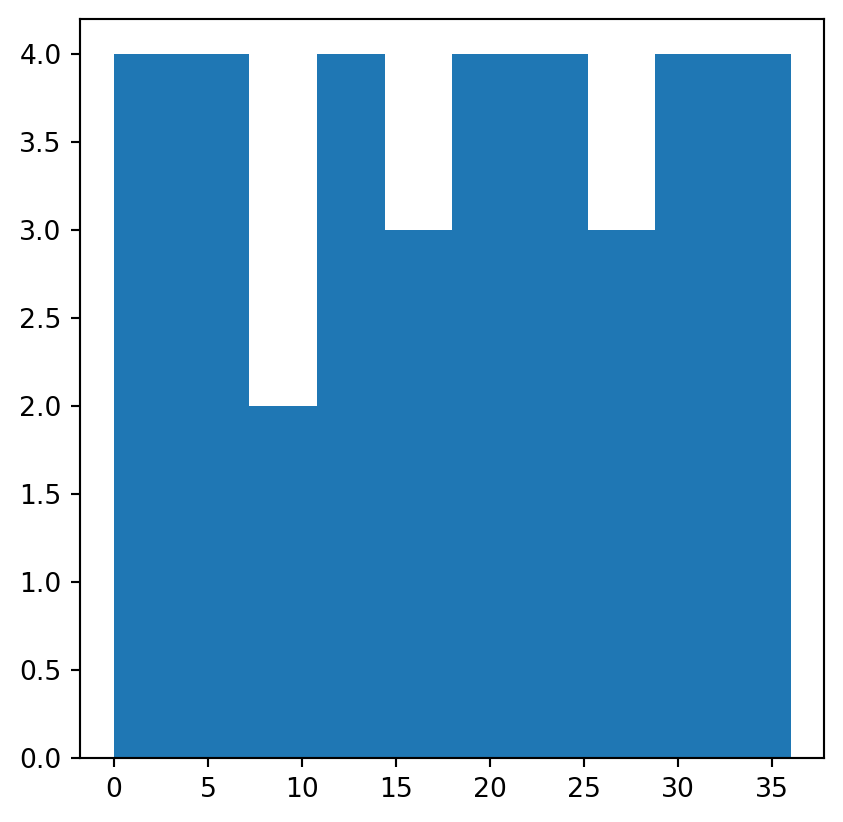
\includegraphics{02-attribute-operations_files/figure-pdf/fig-raster-hist-output-1.pdf}

}

\caption{\label{fig-raster-hist}Distribution of cell values in a
continuous raster (\texttt{elev.tif})}

\end{figure}%

To summarize the distribution of values in a categorical raster, we can
calculate the frequencies of unique values, and draw them using a
barplot. Let's demonstrate using the \texttt{grain.tif} small
categorical raster.

\begin{Shaded}
\begin{Highlighting}[]
\NormalTok{grain }\OperatorTok{=}\NormalTok{ src\_grain.read(}\DecValTok{1}\NormalTok{)}
\NormalTok{grain}
\end{Highlighting}
\end{Shaded}

\begin{verbatim}
array([[1, 0, 1, 2, 2, 2],
       [0, 2, 0, 0, 2, 1],
       [0, 2, 2, 0, 0, 2],
       [0, 0, 1, 1, 1, 1],
       [1, 1, 1, 2, 1, 1],
       [2, 1, 2, 2, 0, 2]], dtype=uint8)
\end{verbatim}

To calculate the frequency of unique values in an array, we use the
\texttt{np.unique} with the \texttt{return\_counts=True} option. The
result is a \texttt{tuple} with two corresponding arrays: the unique
values, and their counts.

\begin{Shaded}
\begin{Highlighting}[]
\NormalTok{freq }\OperatorTok{=}\NormalTok{ np.unique(grain, return\_counts}\OperatorTok{=}\VariableTok{True}\NormalTok{)}
\NormalTok{freq}
\end{Highlighting}
\end{Shaded}

\begin{verbatim}
(array([0, 1, 2], dtype=uint8), array([10, 13, 13]))
\end{verbatim}

These two arrays can be passed to the \texttt{plt.bar} function to draw
a barplot, as shown in Figure~\ref{fig-raster-bar}.

\begin{Shaded}
\begin{Highlighting}[]
\NormalTok{plt.bar(}\OperatorTok{*}\NormalTok{freq)}\OperatorTok{;}
\end{Highlighting}
\end{Shaded}

\begin{figure}[H]

\centering{

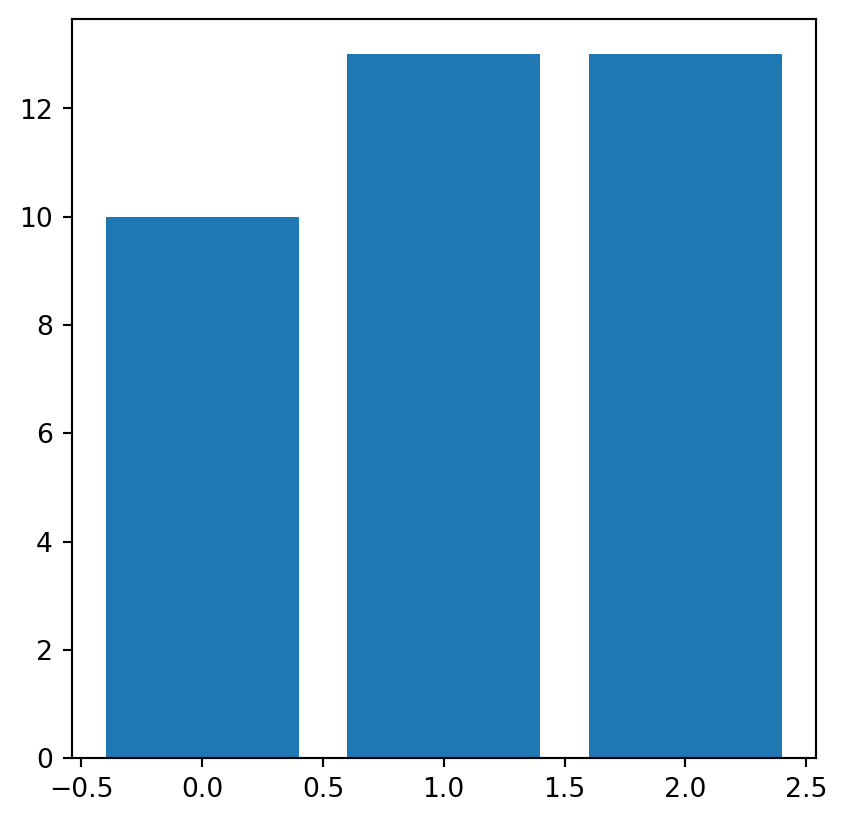
\includegraphics{02-attribute-operations_files/figure-pdf/fig-raster-bar-output-1.pdf}

}

\caption{\label{fig-raster-bar}Distribution of cell values in
categorical raster (\texttt{grain.tif})}

\end{figure}%

\bookmarksetup{startatroot}

\chapter{Spatial data operations}\label{sec-spatial-operations}

\section*{Prerequisites}\label{prerequisites-2}
\addcontentsline{toc}{section}{Prerequisites}

\markright{Prerequisites}

This chapter requires importing the following packages:

\begin{Shaded}
\begin{Highlighting}[]
\ImportTok{import}\NormalTok{ os}
\ImportTok{import}\NormalTok{ numpy }\ImportTok{as}\NormalTok{ np}
\ImportTok{import}\NormalTok{ matplotlib.pyplot }\ImportTok{as}\NormalTok{ plt}
\ImportTok{import}\NormalTok{ pandas }\ImportTok{as}\NormalTok{ pd}
\ImportTok{import}\NormalTok{ scipy.ndimage}
\ImportTok{import}\NormalTok{ scipy.stats}
\ImportTok{import}\NormalTok{ shapely}
\ImportTok{import}\NormalTok{ geopandas }\ImportTok{as}\NormalTok{ gpd}
\ImportTok{import}\NormalTok{ rasterio}
\ImportTok{import}\NormalTok{ rasterio.plot}
\ImportTok{import}\NormalTok{ rasterio.merge}
\ImportTok{import}\NormalTok{ rasterio.features}
\end{Highlighting}
\end{Shaded}

It also relies on the following data files:

\begin{Shaded}
\begin{Highlighting}[]
\NormalTok{nz }\OperatorTok{=}\NormalTok{ gpd.read\_file(}\StringTok{\textquotesingle{}data/nz.gpkg\textquotesingle{}}\NormalTok{)}
\NormalTok{nz\_height }\OperatorTok{=}\NormalTok{ gpd.read\_file(}\StringTok{\textquotesingle{}data/nz\_height.gpkg\textquotesingle{}}\NormalTok{)}
\NormalTok{world }\OperatorTok{=}\NormalTok{ gpd.read\_file(}\StringTok{\textquotesingle{}data/world.gpkg\textquotesingle{}}\NormalTok{)}
\NormalTok{cycle\_hire }\OperatorTok{=}\NormalTok{ gpd.read\_file(}\StringTok{\textquotesingle{}data/cycle\_hire.gpkg\textquotesingle{}}\NormalTok{)}
\NormalTok{cycle\_hire\_osm }\OperatorTok{=}\NormalTok{ gpd.read\_file(}\StringTok{\textquotesingle{}data/cycle\_hire\_osm.gpkg\textquotesingle{}}\NormalTok{)}
\NormalTok{src\_elev }\OperatorTok{=}\NormalTok{ rasterio.}\BuiltInTok{open}\NormalTok{(}\StringTok{\textquotesingle{}output/elev.tif\textquotesingle{}}\NormalTok{)}
\NormalTok{src\_landsat }\OperatorTok{=}\NormalTok{ rasterio.}\BuiltInTok{open}\NormalTok{(}\StringTok{\textquotesingle{}data/landsat.tif\textquotesingle{}}\NormalTok{)}
\NormalTok{src\_grain }\OperatorTok{=}\NormalTok{ rasterio.}\BuiltInTok{open}\NormalTok{(}\StringTok{\textquotesingle{}output/grain.tif\textquotesingle{}}\NormalTok{)}
\end{Highlighting}
\end{Shaded}

\section{Introduction}\label{introduction-2}

Spatial operations, including spatial joins between vector datasets and
local and focal operations on raster datasets, are a vital part of
geocomputation. This chapter shows how spatial objects can be modified
in a multitude of ways based on their location and shape. Many spatial
operations have a non-spatial (attribute) equivalent, so concepts such
as subsetting and joining datasets demonstrated in the previous chapter
are applicable here. This is especially true for vector operations:
Section~\ref{sec-vector-attribute-manipulation} on vector attribute
manipulation provides the basis for understanding its spatial
counterpart, namely spatial subsetting (covered in
Section~\ref{sec-spatial-subsetting-vector}). Spatial joining
(Section~\ref{sec-spatial-joining}) and aggregation
(Section~\ref{sec-vector-spatial-aggregation}) also have non-spatial
counterparts, covered in the previous chapter.

Spatial operations differ from non-spatial operations in a number of
ways, however. Spatial joins, for example, can be done in a number of
ways---including matching entities that intersect with or are within a
certain distance of the target dataset---while the attribution joins
discussed in Section~\ref{sec-vector-attribute-joining} in the previous
chapter can only be done in one way. Different types of spatial
relationships between objects, including intersects and disjoints, are
described in Section~\ref{sec-topological-relations}. Another unique
aspect of spatial objects is distance: all spatial objects are related
through space, and distance calculations can be used to explore the
strength of this relationship, as described in the context of vector
data in Section~\ref{sec-distance-relations}.

Spatial operations on raster objects include subsetting---covered in
Section~\ref{sec-spatial-subsetting-raster}---and merging several raster
`tiles' into a single object, as demonstrated in
Section~\ref{sec-merging-rasters}. Map algebra covers a range of
operations that modify raster cell values, with or without reference to
surrounding cell values. The concept of map algebra, vital for many
applications, is introduced in Section~\ref{sec-map-algebra}; local,
focal, and zonal map algebra operations are covered in sections
Section~\ref{sec-raster-local-operations},
Section~\ref{sec-focal-operations}, and
Section~\ref{sec-zonal-operations}, respectively. Global map algebra
operations, which generate summary statistics representing an entire
raster dataset, and distance calculations on rasters, are discussed in
Section Section~\ref{sec-global-operations-and-distances}.

\begin{tcolorbox}[enhanced jigsaw, breakable, title=\textcolor{quarto-callout-note-color}{\faInfo}\hspace{0.5em}{Note}, arc=.35mm, opacitybacktitle=0.6, left=2mm, colback=white, bottomrule=.15mm, bottomtitle=1mm, toptitle=1mm, colframe=quarto-callout-note-color-frame, leftrule=.75mm, rightrule=.15mm, toprule=.15mm, titlerule=0mm, opacityback=0, colbacktitle=quarto-callout-note-color!10!white, coltitle=black]

It is important to note that spatial operations that use two spatial
objects rely on both objects having the same coordinate reference
system, a topic that was introduced in
Section~\ref{sec-coordinate-reference-systems-intro} and which will be
covered in more depth in Chapter~\ref{sec-reproj-geo-data}.

\end{tcolorbox}

\section{Spatial operations on vector data}\label{sec-spatial-vec}

This section provides an overview of spatial operations on vector
geographic data represented as Simple Features using the
\textbf{shapely} and \textbf{geopandas} packages.
Section~\ref{sec-spatial-ras} then presents spatial operations on raster
datasets, using the \textbf{rasterio} and \textbf{scipy} packages.

\subsection{Spatial subsetting}\label{sec-spatial-subsetting-vector}

Spatial subsetting is the process of taking a spatial object and
returning a new object containing only features that relate in space to
another object. Analogous to attribute subsetting (covered in
Section~\ref{sec-vector-attribute-subsetting}), subsets of
\texttt{GeoDataFrame}s can be created with square bracket (\texttt{{[}})
operator using the syntax \texttt{x{[}y{]}}, where \texttt{x} is an
\texttt{GeoDataFrame} from which a subset of rows/features will be
returned, and \texttt{y} is a boolean \texttt{Series}. The difference
is, that, in spatial subsetting \texttt{y} is created based on another
geometry and using one of the binary geometry relation methods, such as
\texttt{.intersects} (see Section~\ref{sec-topological-relations}),
rather than based on comparison based on ordinary columns.

To demonstrate spatial subsetting, we will use the \texttt{nz} and
\texttt{nz\_height} layers, which contain geographic data on the 16 main
regions and 101 highest points in New Zealand, respectively
(Figure~\ref{fig-spatial-subset} (a)), in a projected coordinate system.
The following expression creates a new object, \texttt{canterbury},
representing only one region---Canterbury.

\begin{Shaded}
\begin{Highlighting}[]
\NormalTok{canterbury }\OperatorTok{=}\NormalTok{ nz[nz[}\StringTok{\textquotesingle{}Name\textquotesingle{}}\NormalTok{] }\OperatorTok{==} \StringTok{\textquotesingle{}Canterbury\textquotesingle{}}\NormalTok{]}
\NormalTok{canterbury}
\end{Highlighting}
\end{Shaded}

\begin{longtable}[]{@{}llllll@{}}
\toprule\noalign{}
& Name & Island & ... & Sex\_ratio & geometry \\
\midrule\noalign{}
\endhead
\bottomrule\noalign{}
\endlastfoot
10 & Canterbury & South & ... & 0.975327 & MULTIPOLYGON (((1686901.914
535... \\
\end{longtable}

Then, we use the \texttt{.intersects} method to evaluate, for each of
the \texttt{nz\_height} points, whether they intersect with Canterbury.
The result \texttt{canterbury\_height} is a boolean \texttt{Series} with
the `answers'.

\begin{Shaded}
\begin{Highlighting}[]
\NormalTok{sel }\OperatorTok{=}\NormalTok{ nz\_height.intersects(canterbury.geometry.iloc[}\DecValTok{0}\NormalTok{])}
\NormalTok{sel}
\end{Highlighting}
\end{Shaded}

\begin{verbatim}
0      False
1      False
2      False
       ...  
98     False
99     False
100    False
Length: 101, dtype: bool
\end{verbatim}

Finally, we can subset \texttt{nz\_height} using the obtained
\texttt{Series}, resulting in the subset \texttt{canterbury\_height}
with only those points that intersect with Canterbury.

\begin{Shaded}
\begin{Highlighting}[]
\NormalTok{canterbury\_height }\OperatorTok{=}\NormalTok{ nz\_height[sel]}
\NormalTok{canterbury\_height}
\end{Highlighting}
\end{Shaded}

\begin{longtable}[]{@{}llll@{}}
\toprule\noalign{}
& t50\_fid & elevation & geometry \\
\midrule\noalign{}
\endhead
\bottomrule\noalign{}
\endlastfoot
4 & 2362630 & 2749 & POINT (1378169.6 5158491.453) \\
5 & 2362814 & 2822 & POINT (1389460.041 5168749.086) \\
6 & 2362817 & 2778 & POINT (1390166.225 5169466.158) \\
... & ... & ... & ... \\
92 & 2380298 & 2877 & POINT (1652788.127 5348984.469) \\
93 & 2380300 & 2711 & POINT (1654213.379 5349962.973) \\
94 & 2380308 & 2885 & POINT (1654898.622 5350462.779) \\
\end{longtable}

Figure~\ref{fig-spatial-subset} compares the original
\texttt{nz\_height} layer (left) with the subset
\texttt{canterbury\_height} (right).

\begin{Shaded}
\begin{Highlighting}[]
\CommentTok{\# Original}
\NormalTok{base }\OperatorTok{=}\NormalTok{ nz.plot(color}\OperatorTok{=}\StringTok{\textquotesingle{}white\textquotesingle{}}\NormalTok{, edgecolor}\OperatorTok{=}\StringTok{\textquotesingle{}lightgrey\textquotesingle{}}\NormalTok{)}
\NormalTok{nz\_height.plot(ax}\OperatorTok{=}\NormalTok{base, color}\OperatorTok{=}\StringTok{\textquotesingle{}None\textquotesingle{}}\NormalTok{, edgecolor}\OperatorTok{=}\StringTok{\textquotesingle{}red\textquotesingle{}}\NormalTok{)}\OperatorTok{;}
\CommentTok{\# Subset (intersects)}
\NormalTok{base }\OperatorTok{=}\NormalTok{ nz.plot(color}\OperatorTok{=}\StringTok{\textquotesingle{}white\textquotesingle{}}\NormalTok{, edgecolor}\OperatorTok{=}\StringTok{\textquotesingle{}lightgrey\textquotesingle{}}\NormalTok{)}
\NormalTok{canterbury.plot(ax}\OperatorTok{=}\NormalTok{base, color}\OperatorTok{=}\StringTok{\textquotesingle{}lightgrey\textquotesingle{}}\NormalTok{, edgecolor}\OperatorTok{=}\StringTok{\textquotesingle{}darkgrey\textquotesingle{}}\NormalTok{)}
\NormalTok{canterbury\_height.plot(ax}\OperatorTok{=}\NormalTok{base, color}\OperatorTok{=}\StringTok{\textquotesingle{}None\textquotesingle{}}\NormalTok{, edgecolor}\OperatorTok{=}\StringTok{\textquotesingle{}red\textquotesingle{}}\NormalTok{)}\OperatorTok{;}
\end{Highlighting}
\end{Shaded}

\begin{figure}

\begin{minipage}{0.50\linewidth}

\centering{

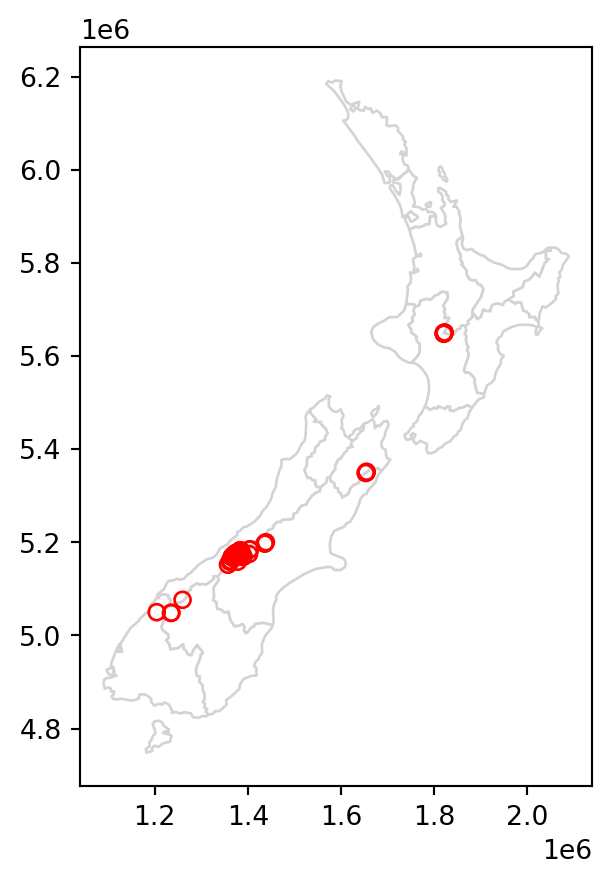
\includegraphics{03-spatial-operations_files/figure-pdf/fig-spatial-subset-output-1.pdf}

}

\subcaption{\label{fig-spatial-subset-1}Original points (red)}

\end{minipage}%
%
\begin{minipage}{0.50\linewidth}

\centering{

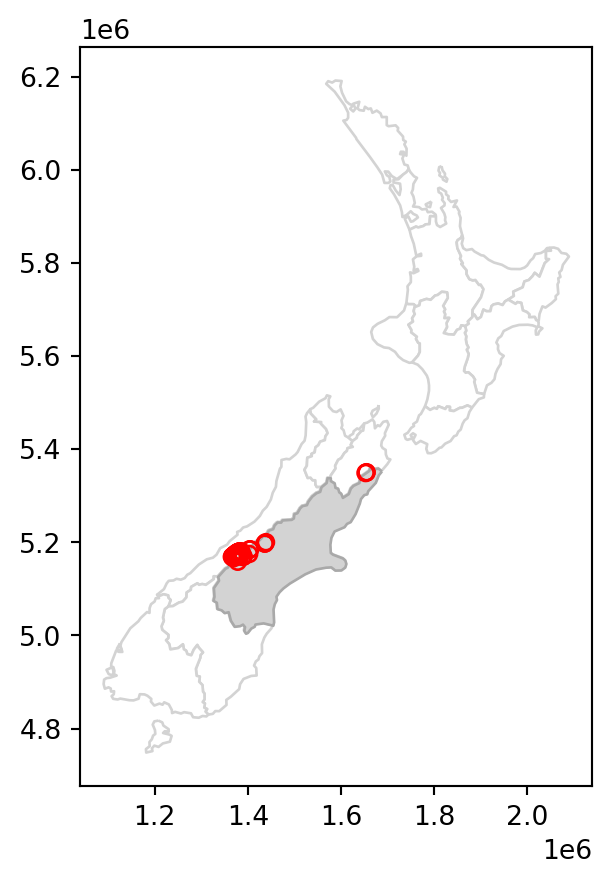
\includegraphics{03-spatial-operations_files/figure-pdf/fig-spatial-subset-output-2.pdf}

}

\subcaption{\label{fig-spatial-subset-2}Spatial subset based on
intersection (red), geometry used for subsetting (Canterbury) (grey)}

\end{minipage}%

\caption{\label{fig-spatial-subset}Spatial subsetting of points by
intersection with polygon}

\end{figure}%

Like in attribute subsetting
(Section~\ref{sec-vector-attribute-subsetting}), we are using a boolean
series (\texttt{sel}), of the same length as the number of rows in the
filtered table (\texttt{nz\_height}), created based on a condition
applied on itself. The difference is that the condition is not a
comparison of attribute values, but an evaluation of a spatial relation.
Namely, we evaluate whether each geometry of \texttt{nz\_height}
intersects with the \texttt{canterbury} geometry, using the
\texttt{.intersects} method.

Various topological relations can be used for spatial subsetting which
determine the type of spatial relationship that features in the target
object must have with the subsetting object to be selected. These
include touches, crosses, or within, as we will see shortly in
Section~\ref{sec-topological-relations}. Intersects
(\texttt{.intersects}), which we used in the last example, is the most
commonly used method. This is a `catch all' topological relation, that
will return features in the target that touch, cross or are within the
source `subsetting' object. As an example of another method, we can use
\texttt{.disjoint} to obtain all points that \emph{do not} intersect
with Canterbury.

\begin{Shaded}
\begin{Highlighting}[]
\NormalTok{sel }\OperatorTok{=}\NormalTok{ nz\_height.disjoint(canterbury.geometry.iloc[}\DecValTok{0}\NormalTok{])}
\NormalTok{canterbury\_height2 }\OperatorTok{=}\NormalTok{ nz\_height[sel]}
\end{Highlighting}
\end{Shaded}

The results are shown in Figure~\ref{fig-spatial-subset-disjoint}, which
compares the original \texttt{nz\_height} layer (left) with the subset
\texttt{canterbury\_height2} (right).

\begin{Shaded}
\begin{Highlighting}[]
\CommentTok{\# Original}
\NormalTok{base }\OperatorTok{=}\NormalTok{ nz.plot(color}\OperatorTok{=}\StringTok{\textquotesingle{}white\textquotesingle{}}\NormalTok{, edgecolor}\OperatorTok{=}\StringTok{\textquotesingle{}lightgrey\textquotesingle{}}\NormalTok{)}
\NormalTok{nz\_height.plot(ax}\OperatorTok{=}\NormalTok{base, color}\OperatorTok{=}\StringTok{\textquotesingle{}None\textquotesingle{}}\NormalTok{, edgecolor}\OperatorTok{=}\StringTok{\textquotesingle{}red\textquotesingle{}}\NormalTok{)}\OperatorTok{;}
\CommentTok{\# Subset (disjoint)}
\NormalTok{base }\OperatorTok{=}\NormalTok{ nz.plot(color}\OperatorTok{=}\StringTok{\textquotesingle{}white\textquotesingle{}}\NormalTok{, edgecolor}\OperatorTok{=}\StringTok{\textquotesingle{}lightgrey\textquotesingle{}}\NormalTok{)}
\NormalTok{canterbury.plot(ax}\OperatorTok{=}\NormalTok{base, color}\OperatorTok{=}\StringTok{\textquotesingle{}lightgrey\textquotesingle{}}\NormalTok{, edgecolor}\OperatorTok{=}\StringTok{\textquotesingle{}darkgrey\textquotesingle{}}\NormalTok{)}
\NormalTok{canterbury\_height2.plot(ax}\OperatorTok{=}\NormalTok{base, color}\OperatorTok{=}\StringTok{\textquotesingle{}None\textquotesingle{}}\NormalTok{, edgecolor}\OperatorTok{=}\StringTok{\textquotesingle{}red\textquotesingle{}}\NormalTok{)}\OperatorTok{;}
\end{Highlighting}
\end{Shaded}

\begin{figure}

\begin{minipage}{0.50\linewidth}

\centering{

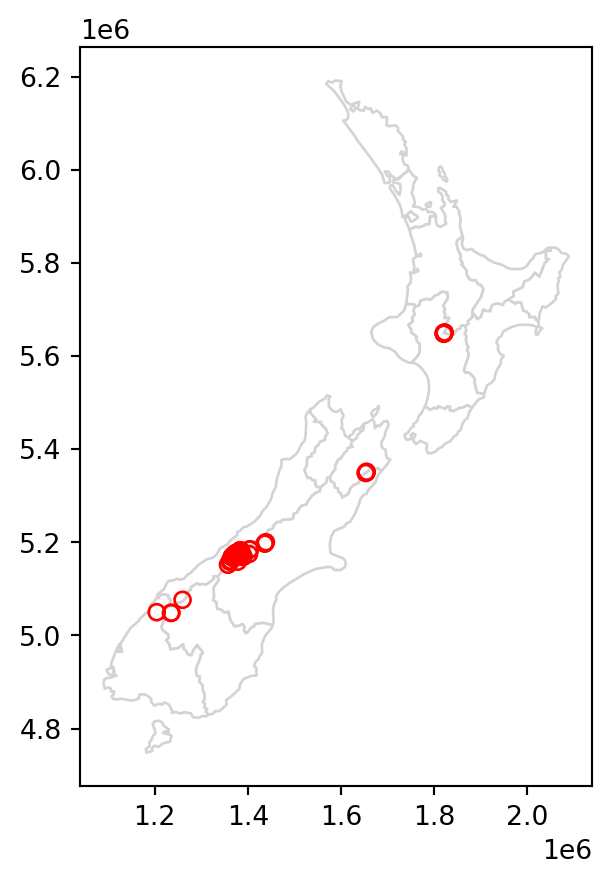
\includegraphics{03-spatial-operations_files/figure-pdf/fig-spatial-subset-disjoint-output-1.pdf}

}

\subcaption{\label{fig-spatial-subset-disjoint-1}Original points (red)}

\end{minipage}%
%
\begin{minipage}{0.50\linewidth}

\centering{

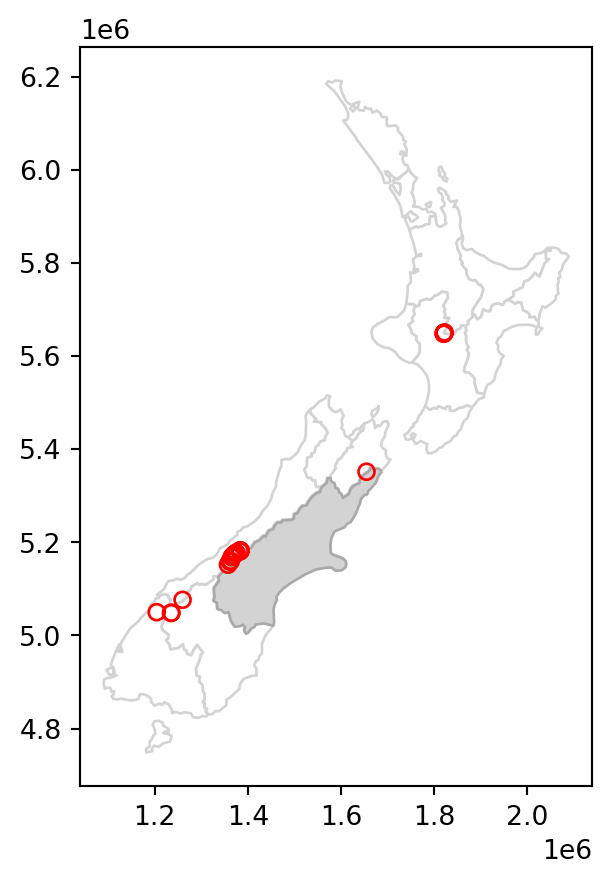
\includegraphics{03-spatial-operations_files/figure-pdf/fig-spatial-subset-disjoint-output-2.pdf}

}

\subcaption{\label{fig-spatial-subset-disjoint-2}Spatial subset based on
disjoint (red), geometry used for subsetting (Canterbury) (grey)}

\end{minipage}%

\caption{\label{fig-spatial-subset-disjoint}Spatial subsetting of points
disjoint from a polygon}

\end{figure}%

In case we need to subset according to several geometries at once, e.g.,
find out which points intersect with both Canterbury and Southland, we
can dissolve the filtering subset, using \texttt{.union\_all}, before
applying the \texttt{.intersects} (or any other) operator. For example,
here is how we can subset the \texttt{nz\_height} points which intersect
with Canterbury or Southland. (Note that we are also using the
\texttt{.isin} method, as demonstrated at the end of
Section~\ref{sec-vector-attribute-subsetting}.)

\begin{Shaded}
\begin{Highlighting}[]
\NormalTok{canterbury\_southland }\OperatorTok{=}\NormalTok{ nz[nz[}\StringTok{\textquotesingle{}Name\textquotesingle{}}\NormalTok{].isin([}\StringTok{\textquotesingle{}Canterbury\textquotesingle{}}\NormalTok{, }\StringTok{\textquotesingle{}Southland\textquotesingle{}}\NormalTok{])]}
\NormalTok{sel }\OperatorTok{=}\NormalTok{ nz\_height.intersects(canterbury\_southland.union\_all())}
\NormalTok{canterbury\_southland\_height }\OperatorTok{=}\NormalTok{ nz\_height[sel]}
\NormalTok{canterbury\_southland\_height}
\end{Highlighting}
\end{Shaded}

\begin{longtable}[]{@{}llll@{}}
\toprule\noalign{}
& t50\_fid & elevation & geometry \\
\midrule\noalign{}
\endhead
\bottomrule\noalign{}
\endlastfoot
0 & 2353944 & 2723 & POINT (1204142.603 5049971.287) \\
4 & 2362630 & 2749 & POINT (1378169.6 5158491.453) \\
5 & 2362814 & 2822 & POINT (1389460.041 5168749.086) \\
... & ... & ... & ... \\
92 & 2380298 & 2877 & POINT (1652788.127 5348984.469) \\
93 & 2380300 & 2711 & POINT (1654213.379 5349962.973) \\
94 & 2380308 & 2885 & POINT (1654898.622 5350462.779) \\
\end{longtable}

Figure~\ref{fig-spatial-subset2} shows the results of the spatial
subsetting of \texttt{nz\_height} points by intersection with Canterbury
and Southland.

\begin{Shaded}
\begin{Highlighting}[]
\CommentTok{\# Original}
\NormalTok{base }\OperatorTok{=}\NormalTok{ nz.plot(color}\OperatorTok{=}\StringTok{\textquotesingle{}white\textquotesingle{}}\NormalTok{, edgecolor}\OperatorTok{=}\StringTok{\textquotesingle{}lightgrey\textquotesingle{}}\NormalTok{)}
\NormalTok{nz\_height.plot(ax}\OperatorTok{=}\NormalTok{base, color}\OperatorTok{=}\StringTok{\textquotesingle{}None\textquotesingle{}}\NormalTok{, edgecolor}\OperatorTok{=}\StringTok{\textquotesingle{}red\textquotesingle{}}\NormalTok{)}\OperatorTok{;}
\CommentTok{\# Subset by intersection with two polygons}
\NormalTok{base }\OperatorTok{=}\NormalTok{ nz.plot(color}\OperatorTok{=}\StringTok{\textquotesingle{}white\textquotesingle{}}\NormalTok{, edgecolor}\OperatorTok{=}\StringTok{\textquotesingle{}lightgrey\textquotesingle{}}\NormalTok{)}
\NormalTok{canterbury\_southland.plot(ax}\OperatorTok{=}\NormalTok{base, color}\OperatorTok{=}\StringTok{\textquotesingle{}lightgrey\textquotesingle{}}\NormalTok{, edgecolor}\OperatorTok{=}\StringTok{\textquotesingle{}darkgrey\textquotesingle{}}\NormalTok{)}
\NormalTok{canterbury\_southland\_height.plot(ax}\OperatorTok{=}\NormalTok{base, color}\OperatorTok{=}\StringTok{\textquotesingle{}None\textquotesingle{}}\NormalTok{, edgecolor}\OperatorTok{=}\StringTok{\textquotesingle{}red\textquotesingle{}}\NormalTok{)}\OperatorTok{;}
\end{Highlighting}
\end{Shaded}

\begin{figure}

\begin{minipage}{0.50\linewidth}

\centering{

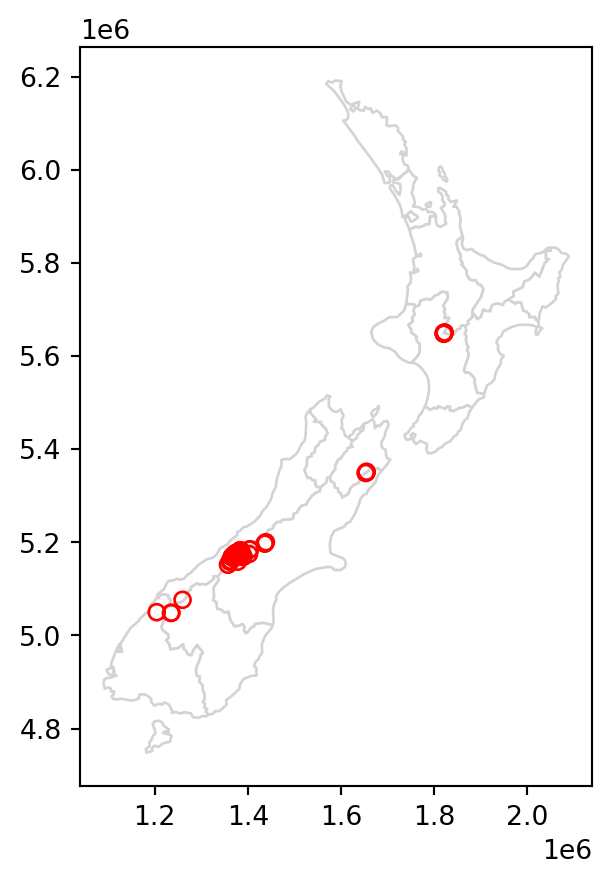
\includegraphics{03-spatial-operations_files/figure-pdf/fig-spatial-subset2-output-1.pdf}

}

\subcaption{\label{fig-spatial-subset2-1}Original points (red)}

\end{minipage}%
%
\begin{minipage}{0.50\linewidth}

\centering{

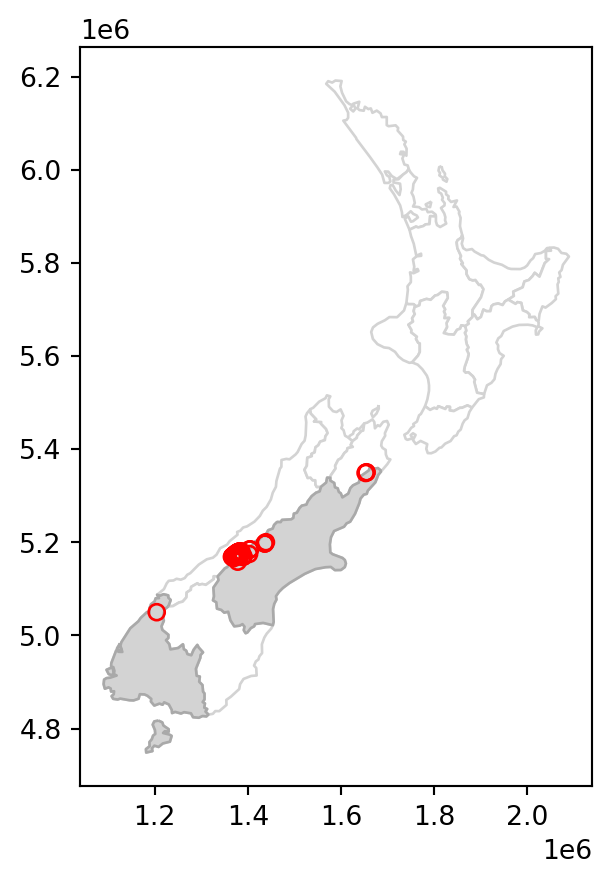
\includegraphics{03-spatial-operations_files/figure-pdf/fig-spatial-subset2-output-2.pdf}

}

\subcaption{\label{fig-spatial-subset2-2}Spatial subset based on
intersection (red), geometry used for subsetting (Canterbury and
Southland) (grey)}

\end{minipage}%

\caption{\label{fig-spatial-subset2}Spatial subsetting of points by
intersection with more than one polygon}

\end{figure}%

The next section further explores different types of spatial relations,
also known as binary predicates (of which \texttt{.intersects} and
\texttt{.disjoint} are two examples), that can be used to identify
whether or not two features are spatially related.

\subsection{Topological relations}\label{sec-topological-relations}

Topological relations describe the spatial relationships between
objects. `Binary topological relationships', to give them their full
name, are logical statements (in that the answer can only be
\texttt{True} or \texttt{False}) about the spatial relationships between
two objects defined by ordered sets of points (typically forming points,
lines, and polygons) in two or more dimensions (Egenhofer and Herring
1990). That may sound rather abstract and, indeed, the definition and
classification of topological relations is based on mathematical
foundations first published in book form in 1966 (Spanier 1995), with
the field of algebraic topology continuing into the 21st century (Dieck
2008).

Despite their mathematical origins, topological relations can be
understood intuitively with reference to visualizations of commonly used
functions that test for common types of spatial relationships.
Figure~\ref{fig-spatial-relations} shows a variety of geometry pairs and
their associated relations. The third and fourth pairs in
Figure~\ref{fig-spatial-relations} (from left to right and then down)
demonstrate that, for some relations, order is important: while the
relations equals, intersects, crosses, touches and overlaps are
symmetrical, meaning that if \texttt{x.relation(y)} is true,
\texttt{y.relation(x)} will also be true, relations in which the order
of the geometries are important such as contains and within are not.

\begin{tcolorbox}[enhanced jigsaw, breakable, title=\textcolor{quarto-callout-note-color}{\faInfo}\hspace{0.5em}{Note}, arc=.35mm, opacitybacktitle=0.6, left=2mm, colback=white, bottomrule=.15mm, bottomtitle=1mm, toptitle=1mm, colframe=quarto-callout-note-color-frame, leftrule=.75mm, rightrule=.15mm, toprule=.15mm, titlerule=0mm, opacityback=0, colbacktitle=quarto-callout-note-color!10!white, coltitle=black]

Notice that each geometry pair has a `DE-9IM'\footnotemark{} string such
as \texttt{FF2F11212}. DE-9IM strings describe the dimensionality
(0=points, 1=lines, 2=polygons) of the pairwise intersections of the
interior, boundary, and exterior, of two geometries (i.e., nine values
of 0/1/2 encoded into a string). This is an advanced topic beyond the
scope of this book, which can be useful to understand the difference
between relation types, or define custom types of relations. See the
DE-9IM strings section in Geocomputation with R (Lovelace, Nowosad, and
Muenchow 2019). Also note that the \textbf{shapely} package contains the
\texttt{.relate} and \texttt{.relate\_pattern} methods, to derive and to
test for DE-9IM patterns, respectively.

\end{tcolorbox}

\footnotetext{\url{https://en.wikipedia.org/wiki/DE-9IM}}

\begin{figure}

\centering{

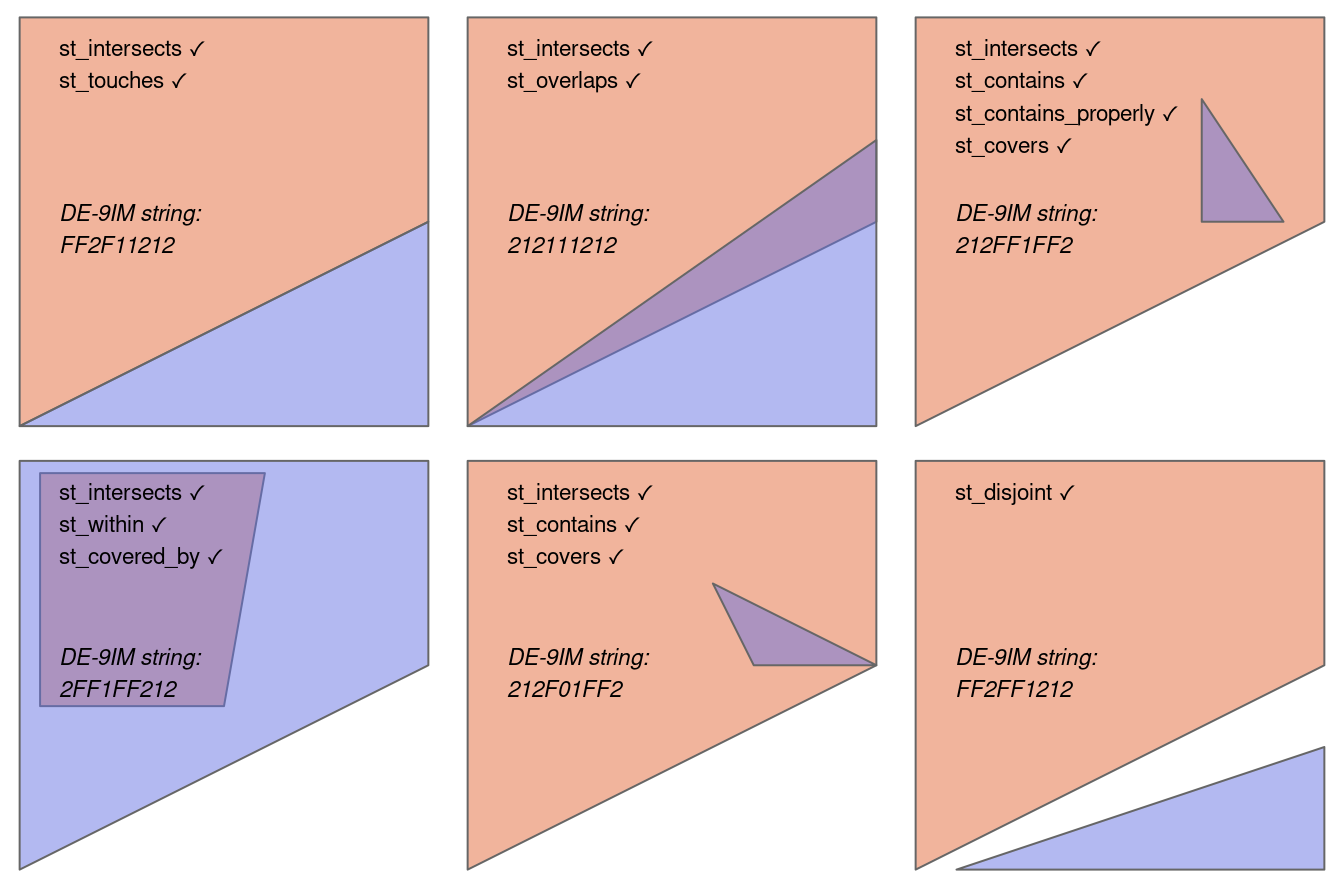
\includegraphics{images/relations-1.png}

}

\caption{\label{fig-spatial-relations}Topological relations between
vector geometries, inspired by Figures 1 and 2 in Egenhofer and Herring
(1990). The relations for which the \texttt{x.relation(y)} is true are
printed for each geometry pair, with \texttt{x} represented in pink and
\texttt{y} represented in blue. The nature of the spatial relationship
for each pair is described by the Dimensionally Extended 9-Intersection
Model string.}

\end{figure}%

In \textbf{shapely}, methods testing for different types of topological
relations are known as `relationships'. \textbf{geopandas} provides
their wrappers (with the same method name) which can be applied on
multiple geometries at once (such as \texttt{.intersects} and
\texttt{.disjoint} applied on all points in \texttt{nz\_height}, see
Section~\ref{sec-spatial-subsetting-vector}). To see how topological
relations work in practice, let's create a simple reproducible example,
building on the relations illustrated in
Figure~\ref{fig-spatial-relations} and consolidating knowledge of how
vector geometries are represented from a previous chapter
(Section~\ref{sec-geometry-columns} and Section~\ref{sec-geometries}).

\begin{Shaded}
\begin{Highlighting}[]
\NormalTok{points }\OperatorTok{=}\NormalTok{ gpd.GeoSeries([}
\NormalTok{  shapely.Point(}\FloatTok{0.2}\NormalTok{,}\FloatTok{0.1}\NormalTok{), }
\NormalTok{  shapely.Point(}\FloatTok{0.7}\NormalTok{,}\FloatTok{0.2}\NormalTok{), }
\NormalTok{  shapely.Point(}\FloatTok{0.4}\NormalTok{,}\FloatTok{0.8}\NormalTok{)}
\NormalTok{])}
\NormalTok{line }\OperatorTok{=}\NormalTok{ gpd.GeoSeries([}
\NormalTok{  shapely.LineString([(}\FloatTok{0.4}\NormalTok{,}\FloatTok{0.2}\NormalTok{), (}\DecValTok{1}\NormalTok{,}\FloatTok{0.5}\NormalTok{)])}
\NormalTok{])}
\NormalTok{poly }\OperatorTok{=}\NormalTok{ gpd.GeoSeries([}
\NormalTok{  shapely.Polygon([(}\DecValTok{0}\NormalTok{,}\DecValTok{0}\NormalTok{), (}\DecValTok{0}\NormalTok{,}\DecValTok{1}\NormalTok{), (}\DecValTok{1}\NormalTok{,}\DecValTok{1}\NormalTok{), (}\DecValTok{1}\NormalTok{,}\FloatTok{0.5}\NormalTok{), (}\DecValTok{0}\NormalTok{,}\DecValTok{0}\NormalTok{)])}
\NormalTok{])}
\end{Highlighting}
\end{Shaded}

The sample dataset which we created is composed of three
\texttt{GeoSeries}: named \texttt{points}, \texttt{line}, and
\texttt{poly}, which are visualized in
Figure~\ref{fig-spatial-relations-geoms}. The last expression is a
\texttt{for} loop used to add text labels (\texttt{0}, \texttt{1}, and
\texttt{2}) to identify the points; we are going to explain the concepts
of text annotations with \textbf{geopandas} \texttt{.plot} in
Section~\ref{sec-plot-static-labels}.

\begin{Shaded}
\begin{Highlighting}[]
\NormalTok{base }\OperatorTok{=}\NormalTok{ poly.plot(color}\OperatorTok{=}\StringTok{\textquotesingle{}lightgrey\textquotesingle{}}\NormalTok{, edgecolor}\OperatorTok{=}\StringTok{\textquotesingle{}red\textquotesingle{}}\NormalTok{)}
\NormalTok{line.plot(ax}\OperatorTok{=}\NormalTok{base, color}\OperatorTok{=}\StringTok{\textquotesingle{}black\textquotesingle{}}\NormalTok{, linewidth}\OperatorTok{=}\DecValTok{7}\NormalTok{)}
\NormalTok{points.plot(ax}\OperatorTok{=}\NormalTok{base, color}\OperatorTok{=}\StringTok{\textquotesingle{}none\textquotesingle{}}\NormalTok{, edgecolor}\OperatorTok{=}\StringTok{\textquotesingle{}black\textquotesingle{}}\NormalTok{)}
\ControlFlowTok{for}\NormalTok{ i }\KeywordTok{in} \BuiltInTok{enumerate}\NormalTok{(points):}
\NormalTok{    base.annotate(}
\NormalTok{        i[}\DecValTok{0}\NormalTok{], xy}\OperatorTok{=}\NormalTok{(i[}\DecValTok{1}\NormalTok{].x, i[}\DecValTok{1}\NormalTok{].y), }
\NormalTok{        xytext}\OperatorTok{=}\NormalTok{(}\DecValTok{3}\NormalTok{, }\DecValTok{3}\NormalTok{), textcoords}\OperatorTok{=}\StringTok{\textquotesingle{}offset points\textquotesingle{}}\NormalTok{, weight}\OperatorTok{=}\StringTok{\textquotesingle{}bold\textquotesingle{}}
\NormalTok{    )}
\end{Highlighting}
\end{Shaded}

\begin{figure}[H]

\centering{

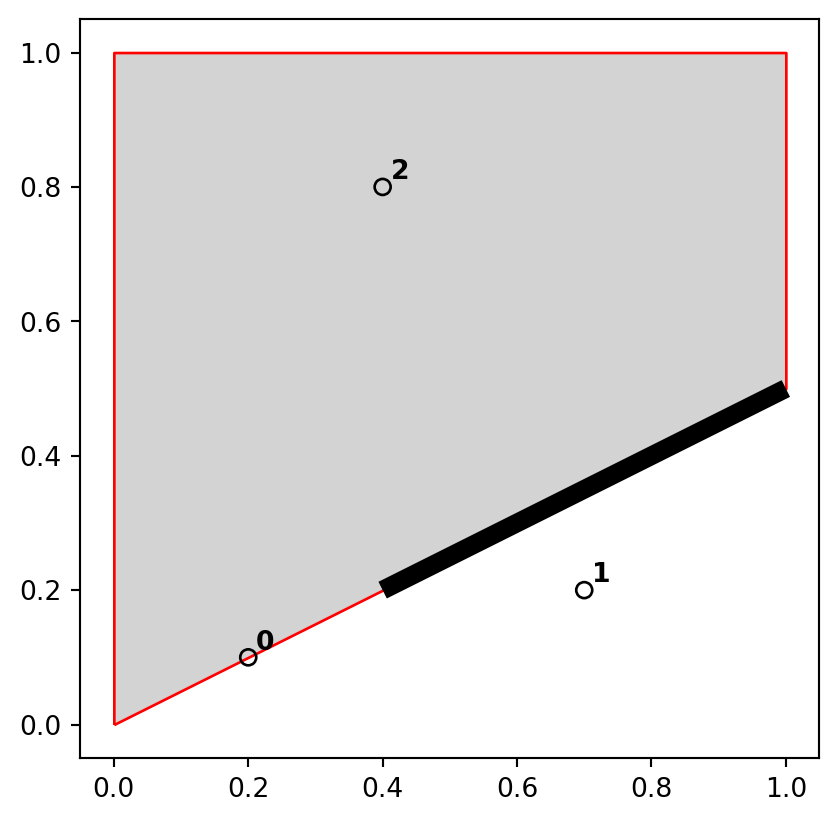
\includegraphics{03-spatial-operations_files/figure-pdf/fig-spatial-relations-geoms-output-1.pdf}

}

\caption{\label{fig-spatial-relations-geoms}Points (\texttt{points}),
line (\texttt{line}), and polygon (\texttt{poly}) objects used to
illustrate topological relations}

\end{figure}%

A simple query is: which of the points in \texttt{points} intersect in
some way with polygon \texttt{poly}? The question can be answered by
visual inspection (points \texttt{0} and \texttt{2} are touching and are
within the polygon, respectively). Alternatively, we can get the
solution with the \texttt{.intersects} method, which reports whether or
not each geometry in a \texttt{GeoSeries} (\texttt{points}) intersects
with a single \texttt{shapely} geometry (\texttt{poly.iloc{[}0{]}}).

\begin{Shaded}
\begin{Highlighting}[]
\NormalTok{points.intersects(poly.iloc[}\DecValTok{0}\NormalTok{])}
\end{Highlighting}
\end{Shaded}

\begin{verbatim}
0     True
1    False
2     True
dtype: bool
\end{verbatim}

The result shown above is a boolean \texttt{Series}. Its contents should
match our intuition: positive (\texttt{True}) results are returned for
the points \texttt{0} and \texttt{2}, and a negative result
(\texttt{False}) for point \texttt{1}. Each value in this
\texttt{Series} represents a feature in the first input
(\texttt{points}).

All earlier examples in this chapter demonstrate the `many-to-one' mode
of \texttt{.intersects} and analogous methods, where the relation is
evaluated between each of several geometries in a
\texttt{GeoSeries}/\texttt{GeoDataFrame}, and an individual
\texttt{shapely} geometry. A second mode of those methods (not
demonstrated here) is when both inputs are
\texttt{GeoSeries}/\texttt{GeoDataFrame} objects. In such case, a
`pairwise' evaluation takes place between geometries aligned by index
(\texttt{align=True}, the default) or by position
(\texttt{align=False}). For example, the expression
\texttt{nz.intersects(nz)} returns a \texttt{Series} of 16 \texttt{True}
values, indicating (unsurprisingly) that each geometry in \texttt{nz}
intersects with itself.

A third mode is when we are interested in a `many-to-many' evaluation,
i.e., obtaining a matrix of all pairwise combinations of geometries from
two \texttt{GeoSeries} objects. At the time of writing, there is no
built-in method to do this in \textbf{geopandas}. However, the
\texttt{.apply} method (package \textbf{pandas}) can be used to repeat a
`many-to-one' evaluation over all geometries in the second layer,
resulting in a matrix of \emph{pairwise} results. We will create another
\texttt{GeoSeries} with two polygons, named \texttt{poly2}, to
demonstrate this.

\begin{Shaded}
\begin{Highlighting}[]
\NormalTok{poly2 }\OperatorTok{=}\NormalTok{ gpd.GeoSeries([}
\NormalTok{  shapely.Polygon([(}\DecValTok{0}\NormalTok{,}\DecValTok{0}\NormalTok{), (}\DecValTok{0}\NormalTok{,}\DecValTok{1}\NormalTok{), (}\DecValTok{1}\NormalTok{,}\DecValTok{1}\NormalTok{), (}\DecValTok{1}\NormalTok{,}\FloatTok{0.5}\NormalTok{), (}\DecValTok{0}\NormalTok{,}\DecValTok{0}\NormalTok{)]),}
\NormalTok{  shapely.Polygon([(}\DecValTok{0}\NormalTok{,}\DecValTok{0}\NormalTok{), (}\DecValTok{1}\NormalTok{,}\FloatTok{0.5}\NormalTok{), (}\DecValTok{1}\NormalTok{,}\DecValTok{0}\NormalTok{), (}\DecValTok{0}\NormalTok{,}\DecValTok{0}\NormalTok{)])}
\NormalTok{])}
\end{Highlighting}
\end{Shaded}

Our two input objects, \texttt{points} and \texttt{poly2}, are
illustrated in Figure~\ref{fig-spatial-relations-geoms2}.

\begin{Shaded}
\begin{Highlighting}[]
\NormalTok{base }\OperatorTok{=}\NormalTok{ poly2.plot(color}\OperatorTok{=}\StringTok{\textquotesingle{}lightgrey\textquotesingle{}}\NormalTok{, edgecolor}\OperatorTok{=}\StringTok{\textquotesingle{}red\textquotesingle{}}\NormalTok{)}
\NormalTok{points.plot(ax}\OperatorTok{=}\NormalTok{base, color}\OperatorTok{=}\StringTok{\textquotesingle{}none\textquotesingle{}}\NormalTok{, edgecolor}\OperatorTok{=}\StringTok{\textquotesingle{}black\textquotesingle{}}\NormalTok{)}
\ControlFlowTok{for}\NormalTok{ i }\KeywordTok{in} \BuiltInTok{enumerate}\NormalTok{(points):}
\NormalTok{    base.annotate(}
\NormalTok{        i[}\DecValTok{0}\NormalTok{], xy}\OperatorTok{=}\NormalTok{(i[}\DecValTok{1}\NormalTok{].x, i[}\DecValTok{1}\NormalTok{].y), }
\NormalTok{        xytext}\OperatorTok{=}\NormalTok{(}\DecValTok{3}\NormalTok{, }\DecValTok{3}\NormalTok{), textcoords}\OperatorTok{=}\StringTok{\textquotesingle{}offset points\textquotesingle{}}\NormalTok{, weight}\OperatorTok{=}\StringTok{\textquotesingle{}bold\textquotesingle{}}
\NormalTok{    )}
\end{Highlighting}
\end{Shaded}

\begin{figure}[H]

\centering{

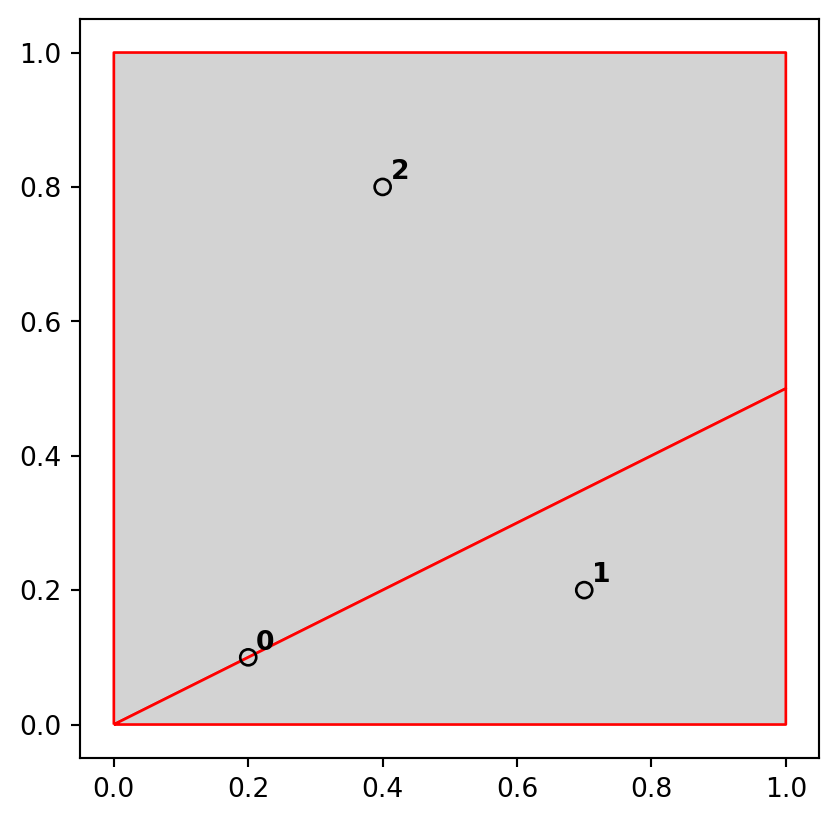
\includegraphics{03-spatial-operations_files/figure-pdf/fig-spatial-relations-geoms2-output-1.pdf}

}

\caption{\label{fig-spatial-relations-geoms2}Inputs for demonstrating
the evaluation of all pairwise intersection relations between three
points (\texttt{points}) and two polygons (\texttt{poly2})}

\end{figure}%

Now we can use \texttt{.apply} to get the intersection relations matrix.
The result is a \texttt{DataFrame}, where each row represents a
\texttt{points} geometry and each column represents a \texttt{poly2}
geometry. We can see that the point \texttt{0} intersects with both
polygons, while points \texttt{1} and \texttt{2} intersect with one of
the polygons each.

\begin{Shaded}
\begin{Highlighting}[]
\NormalTok{points.}\BuiltInTok{apply}\NormalTok{(}\KeywordTok{lambda}\NormalTok{ x: poly2.intersects(x))}
\end{Highlighting}
\end{Shaded}

\begin{longtable}[]{@{}lll@{}}
\toprule\noalign{}
& 0 & 1 \\
\midrule\noalign{}
\endhead
\bottomrule\noalign{}
\endlastfoot
0 & True & True \\
1 & False & True \\
2 & True & False \\
\end{longtable}

\begin{tcolorbox}[enhanced jigsaw, breakable, title=\textcolor{quarto-callout-note-color}{\faInfo}\hspace{0.5em}{Note}, arc=.35mm, opacitybacktitle=0.6, left=2mm, colback=white, bottomrule=.15mm, bottomtitle=1mm, toptitle=1mm, colframe=quarto-callout-note-color-frame, leftrule=.75mm, rightrule=.15mm, toprule=.15mm, titlerule=0mm, opacityback=0, colbacktitle=quarto-callout-note-color!10!white, coltitle=black]

The \texttt{.apply} method (package \textbf{pandas}) is used to apply a
function along one of the axes of a \texttt{DataFrame} (or
\texttt{GeoDataFrame}). That is, we can apply a function on all rows
(\texttt{axis=1}) or all columns (\texttt{axis=0}, the default). When
the function being applied returns a single value, the output of
\texttt{.apply} is a \texttt{Series} (e.g., \texttt{.apply(len)} returns
the lengths of all columns, because \texttt{len} returns a single
value). When the function returns a \texttt{Series}, then
\texttt{.apply} returns a \texttt{DataFrame} (such as in the above
example.)

\end{tcolorbox}

\begin{tcolorbox}[enhanced jigsaw, breakable, title=\textcolor{quarto-callout-note-color}{\faInfo}\hspace{0.5em}{Note}, arc=.35mm, opacitybacktitle=0.6, left=2mm, colback=white, bottomrule=.15mm, bottomtitle=1mm, toptitle=1mm, colframe=quarto-callout-note-color-frame, leftrule=.75mm, rightrule=.15mm, toprule=.15mm, titlerule=0mm, opacityback=0, colbacktitle=quarto-callout-note-color!10!white, coltitle=black]

Since the above result, like any pairwise matrix, (1) is composed of
values of the same type, and (2) has no contrasting role for rows and
columns, is may be more convenient to use a plain \textbf{numpy} array
to work with it. In such case, we can use the \texttt{.to\_numpy} method
to go from \texttt{DataFrame} to \texttt{ndarray}.

\begin{Shaded}
\begin{Highlighting}[]
\NormalTok{points.}\BuiltInTok{apply}\NormalTok{(}\KeywordTok{lambda}\NormalTok{ x: poly2.intersects(x)).to\_numpy()}
\end{Highlighting}
\end{Shaded}

\begin{verbatim}
array([[ True,  True],
       [False,  True],
       [ True, False]])
\end{verbatim}

\end{tcolorbox}

The \texttt{.intersects} method returns \texttt{True} even in cases
where the features just touch: intersects is a `catch-all' topological
operation which identifies many types of spatial relations, as
illustrated in Figure~\ref{fig-spatial-relations}. More restrictive
questions include which points lie within the polygon, and which
features are on or contain a shared boundary with it? The first question
can be answered with \texttt{.within}, and the second with
\texttt{.touches}.

\begin{Shaded}
\begin{Highlighting}[]
\NormalTok{points.within(poly.iloc[}\DecValTok{0}\NormalTok{])}
\end{Highlighting}
\end{Shaded}

\begin{verbatim}
0    False
1    False
2     True
dtype: bool
\end{verbatim}

\begin{Shaded}
\begin{Highlighting}[]
\NormalTok{points.touches(poly.iloc[}\DecValTok{0}\NormalTok{])}
\end{Highlighting}
\end{Shaded}

\begin{verbatim}
0     True
1    False
2    False
dtype: bool
\end{verbatim}

Note that although the point \texttt{0} touches the boundary polygon, it
is not within it; point \texttt{2} is within the polygon but does not
touch any part of its border. The opposite of \texttt{.intersects} is
\texttt{.disjoint}, which returns only objects that do not spatially
relate in any way to the selecting object.

\begin{Shaded}
\begin{Highlighting}[]
\NormalTok{points.disjoint(poly.iloc[}\DecValTok{0}\NormalTok{])}
\end{Highlighting}
\end{Shaded}

\begin{verbatim}
0    False
1     True
2    False
dtype: bool
\end{verbatim}

Another useful type of relation is `within distance', where we detect
features that intersect with the target buffered by particular distance.
Buffer distance determines how close target objects need to be before
they are selected. This can be done by literally buffering
(Section~\ref{sec-geometries}) the target geometry, and evaluating
intersection (\texttt{.intersects}). Another way is to calculate the
distances using the \texttt{.distance} method, and then evaluate whether
they are within a threshold distance.

\begin{Shaded}
\begin{Highlighting}[]
\NormalTok{points.distance(poly.iloc[}\DecValTok{0}\NormalTok{]) }\OperatorTok{\textless{}} \FloatTok{0.2}
\end{Highlighting}
\end{Shaded}

\begin{verbatim}
0    True
1    True
2    True
dtype: bool
\end{verbatim}

Note that although point \texttt{1} is more than \texttt{0.2} units of
distance from the nearest vertex of \texttt{poly}, it is still selected
when the distance is set to \texttt{0.2}. This is because distance is
measured to the nearest edge, in this case, the part of the polygon that
lies directly above point 2 in Figure
Figure~\ref{fig-spatial-relations}. We can verify that the actual
distance between point \texttt{1} and the polygon is \texttt{0.13}, as
follows.

\begin{Shaded}
\begin{Highlighting}[]
\NormalTok{points.iloc[}\DecValTok{1}\NormalTok{].distance(poly.iloc[}\DecValTok{0}\NormalTok{])}
\end{Highlighting}
\end{Shaded}

\begin{verbatim}
0.13416407864998736
\end{verbatim}

This is also a good opportunity to repeat that all distance-related
calculations in \textbf{geopandas} (and \textbf{shapely}) assume planar
geometry, and only take into account the coordinate values. It is up to
the user to make sure that all input layers are in the same projected
CRS, so that this type of calculations make sense (see
Section~\ref{sec-geometry-operations-on-projected-and-unprojected-data}
and Section~\ref{sec-when-to-reproject}).

\subsection{Spatial joining}\label{sec-spatial-joining}

Joining two non-spatial datasets uses a shared `key' variable, as
described in Section~\ref{sec-vector-attribute-joining}. Spatial data
joining applies the same concept, but instead relies on spatial
relations, described in the previous section. As with attribute data,
joining adds new columns to the target object (the argument \texttt{x}
in joining functions), from a source object (\texttt{y}).

The following example illustrates the process: imagine you have ten
points randomly distributed across the Earth's surface and you ask, for
the points that are on land, which countries are they in? Implementing
this idea in a reproducible example will build your geographic data
handling skills and show how spatial joins work. The starting point is
to create points that are randomly scattered over the planar surface
that represents Earth's geographic coordinates, in decimal degrees
(Figure~\ref{fig-spatial-join} (a)).

\begin{Shaded}
\begin{Highlighting}[]
\NormalTok{np.random.seed(}\DecValTok{11}\NormalTok{)       }\CommentTok{\#\# set seed for reproducibility}
\NormalTok{bb }\OperatorTok{=}\NormalTok{ world.total\_bounds  }\CommentTok{\#\# the world\textquotesingle{}s bounds}
\NormalTok{x }\OperatorTok{=}\NormalTok{ np.random.uniform(low}\OperatorTok{=}\NormalTok{bb[}\DecValTok{0}\NormalTok{], high}\OperatorTok{=}\NormalTok{bb[}\DecValTok{2}\NormalTok{], size}\OperatorTok{=}\DecValTok{10}\NormalTok{)}
\NormalTok{y }\OperatorTok{=}\NormalTok{ np.random.uniform(low}\OperatorTok{=}\NormalTok{bb[}\DecValTok{1}\NormalTok{], high}\OperatorTok{=}\NormalTok{bb[}\DecValTok{3}\NormalTok{], size}\OperatorTok{=}\DecValTok{10}\NormalTok{)}
\NormalTok{random\_points }\OperatorTok{=}\NormalTok{ gpd.points\_from\_xy(x, y, crs}\OperatorTok{=}\DecValTok{4326}\NormalTok{)}
\NormalTok{random\_points }\OperatorTok{=}\NormalTok{ gpd.GeoDataFrame(\{}\StringTok{\textquotesingle{}geometry\textquotesingle{}}\NormalTok{: random\_points\})}
\NormalTok{random\_points}
\end{Highlighting}
\end{Shaded}

\begin{longtable}[]{@{}ll@{}}
\toprule\noalign{}
& geometry \\
\midrule\noalign{}
\endhead
\bottomrule\noalign{}
\endlastfoot
0 & POINT (-115.10291 36.78178) \\
1 & POINT (-172.98891 -71.02938) \\
2 & POINT (-13.24134 65.23272) \\
... & ... \\
7 & POINT (-4.54623 -69.64082) \\
8 & POINT (159.05039 -34.99599) \\
9 & POINT (126.28622 -62.49509) \\
\end{longtable}

The scenario illustrated in Figure~\ref{fig-spatial-join} shows that the
\texttt{random\_points} object (top left) lacks attribute data, while
the world (top right) has attributes, including country names that are
shown for a sample of countries in the legend. Before creating the
joined dataset, we use spatial subsetting to create
\texttt{world\_random}, which contains only countries that contain
random points, to verify the number of country names returned in the
joined dataset should be four (see Figure~\ref{fig-spatial-join} (b)).

\begin{Shaded}
\begin{Highlighting}[]
\NormalTok{world\_random }\OperatorTok{=}\NormalTok{ world[world.intersects(random\_points.union\_all())]}
\NormalTok{world\_random}
\end{Highlighting}
\end{Shaded}

\begin{longtable}[]{@{}llllll@{}}
\toprule\noalign{}
& iso\_a2 & name\_long & ... & gdpPercap & geometry \\
\midrule\noalign{}
\endhead
\bottomrule\noalign{}
\endlastfoot
4 & US & United States & ... & 51921.984639 & MULTIPOLYGON (((-171.73166
63.7... \\
18 & RU & Russian Federation & ... & 25284.586202 & MULTIPOLYGON (((-180
64.97971, ... \\
52 & ML & Mali & ... & 1865.160622 & MULTIPOLYGON (((-11.51394
12.44... \\
159 & AQ & Antarctica & ... & NaN & MULTIPOLYGON (((-180 -89.9,
179... \\
\end{longtable}

Spatial joins are implemented with \texttt{x.sjoin(y)}, as illustrated
in the code chunk below. The output is the \texttt{random\_joined}
object which is illustrated in Figure~\ref{fig-spatial-join} (c).

\begin{Shaded}
\begin{Highlighting}[]
\NormalTok{random\_joined }\OperatorTok{=}\NormalTok{ random\_points.sjoin(world, how}\OperatorTok{=}\StringTok{\textquotesingle{}left\textquotesingle{}}\NormalTok{)}
\NormalTok{random\_joined}
\end{Highlighting}
\end{Shaded}

\begin{longtable}[]{@{}llllll@{}}
\toprule\noalign{}
& geometry & index\_right & ... & lifeExp & gdpPercap \\
\midrule\noalign{}
\endhead
\bottomrule\noalign{}
\endlastfoot
0 & POINT (-115.10291 36.78178) & 4.0 & ... & 78.841463 &
51921.984639 \\
1 & POINT (-172.98891 -71.02938) & NaN & ... & NaN & NaN \\
2 & POINT (-13.24134 65.23272) & NaN & ... & NaN & NaN \\
... & ... & ... & ... & ... & ... \\
7 & POINT (-4.54623 -69.64082) & NaN & ... & NaN & NaN \\
8 & POINT (159.05039 -34.99599) & NaN & ... & NaN & NaN \\
9 & POINT (126.28622 -62.49509) & NaN & ... & NaN & NaN \\
\end{longtable}

Figure~\ref{fig-spatial-join} shows the input points and countries, the
illustration of intersecting countries, and the join result.

\begin{Shaded}
\begin{Highlighting}[]
\CommentTok{\# Random points}
\NormalTok{base }\OperatorTok{=}\NormalTok{ world.plot(color}\OperatorTok{=}\StringTok{\textquotesingle{}white\textquotesingle{}}\NormalTok{, edgecolor}\OperatorTok{=}\StringTok{\textquotesingle{}lightgrey\textquotesingle{}}\NormalTok{)}
\NormalTok{random\_points.plot(ax}\OperatorTok{=}\NormalTok{base, color}\OperatorTok{=}\StringTok{\textquotesingle{}None\textquotesingle{}}\NormalTok{, edgecolor}\OperatorTok{=}\StringTok{\textquotesingle{}red\textquotesingle{}}\NormalTok{)}\OperatorTok{;}
\CommentTok{\# World countries intersecting with the points}
\NormalTok{base }\OperatorTok{=}\NormalTok{ world.plot(color}\OperatorTok{=}\StringTok{\textquotesingle{}white\textquotesingle{}}\NormalTok{, edgecolor}\OperatorTok{=}\StringTok{\textquotesingle{}lightgrey\textquotesingle{}}\NormalTok{)}
\NormalTok{world\_random.plot(ax}\OperatorTok{=}\NormalTok{base, column}\OperatorTok{=}\StringTok{\textquotesingle{}name\_long\textquotesingle{}}\NormalTok{)}\OperatorTok{;}
\CommentTok{\# Points with joined country names}
\NormalTok{base }\OperatorTok{=}\NormalTok{ world.plot(color}\OperatorTok{=}\StringTok{\textquotesingle{}white\textquotesingle{}}\NormalTok{, edgecolor}\OperatorTok{=}\StringTok{\textquotesingle{}lightgrey\textquotesingle{}}\NormalTok{)}
\NormalTok{random\_joined.geometry.plot(ax}\OperatorTok{=}\NormalTok{base, color}\OperatorTok{=}\StringTok{\textquotesingle{}grey\textquotesingle{}}\NormalTok{)}
\NormalTok{random\_joined.plot(ax}\OperatorTok{=}\NormalTok{base, column}\OperatorTok{=}\StringTok{\textquotesingle{}name\_long\textquotesingle{}}\NormalTok{, legend}\OperatorTok{=}\VariableTok{True}\NormalTok{)}\OperatorTok{;}
\end{Highlighting}
\end{Shaded}

\begin{figure}

\begin{minipage}{0.50\linewidth}

\centering{

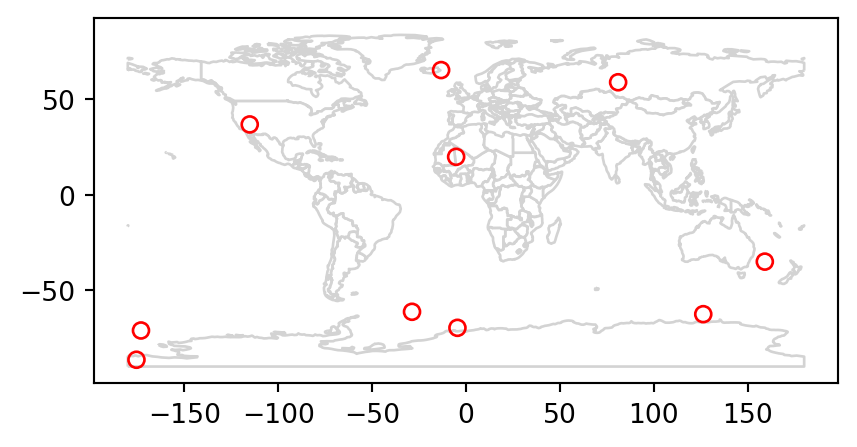
\includegraphics{03-spatial-operations_files/figure-pdf/fig-spatial-join-output-1.pdf}

}

\subcaption{\label{fig-spatial-join-1}A new attribute variable is added
to random points,}

\end{minipage}%
%
\begin{minipage}{0.50\linewidth}

\centering{

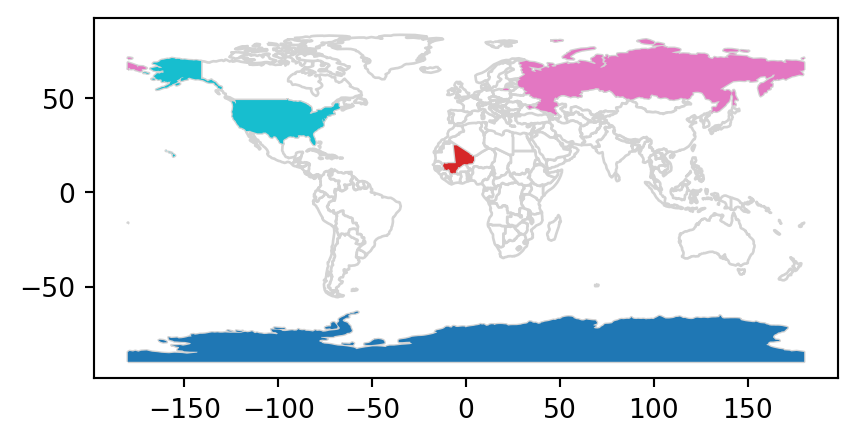
\includegraphics{03-spatial-operations_files/figure-pdf/fig-spatial-join-output-2.pdf}

}

\subcaption{\label{fig-spatial-join-2}from source world object,}

\end{minipage}%
\newline
\begin{minipage}{0.50\linewidth}

\centering{

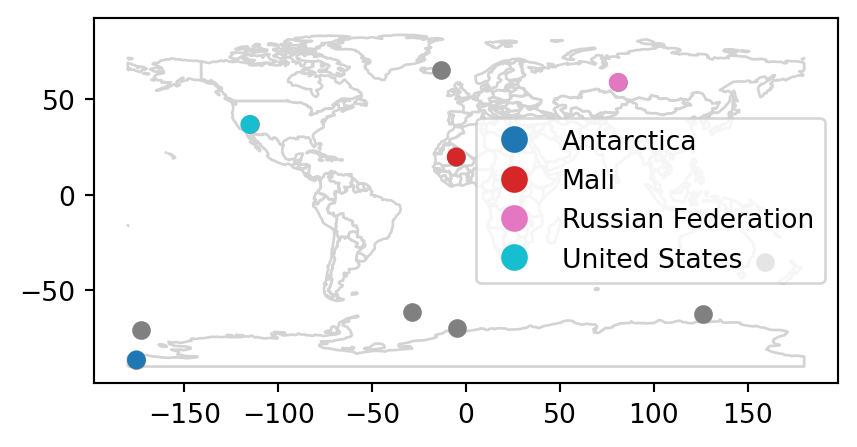
\includegraphics{03-spatial-operations_files/figure-pdf/fig-spatial-join-output-3.pdf}

}

\subcaption{\label{fig-spatial-join-3}resulting in points associated
with country names}

\end{minipage}%

\caption{\label{fig-spatial-join}Illustration of a spatial join}

\end{figure}%

\subsection{Non-overlapping joins}\label{non-overlapping-joins}

Sometimes two geographic datasets do not touch but still have a strong
geographic relationship. The datasets \texttt{cycle\_hire} and
\texttt{cycle\_hire\_osm} provide a good example. Plotting them reveals
that they are often closely related but they do not seem to touch, as
shown in Figure~\ref{fig-cycle-hire}.

\begin{Shaded}
\begin{Highlighting}[]
\NormalTok{base }\OperatorTok{=}\NormalTok{ cycle\_hire.plot(edgecolor}\OperatorTok{=}\StringTok{\textquotesingle{}blue\textquotesingle{}}\NormalTok{, color}\OperatorTok{=}\StringTok{\textquotesingle{}none\textquotesingle{}}\NormalTok{)}
\NormalTok{cycle\_hire\_osm.plot(ax}\OperatorTok{=}\NormalTok{base, edgecolor}\OperatorTok{=}\StringTok{\textquotesingle{}red\textquotesingle{}}\NormalTok{, color}\OperatorTok{=}\StringTok{\textquotesingle{}none\textquotesingle{}}\NormalTok{)}\OperatorTok{;}
\end{Highlighting}
\end{Shaded}

\begin{figure}[H]

\centering{

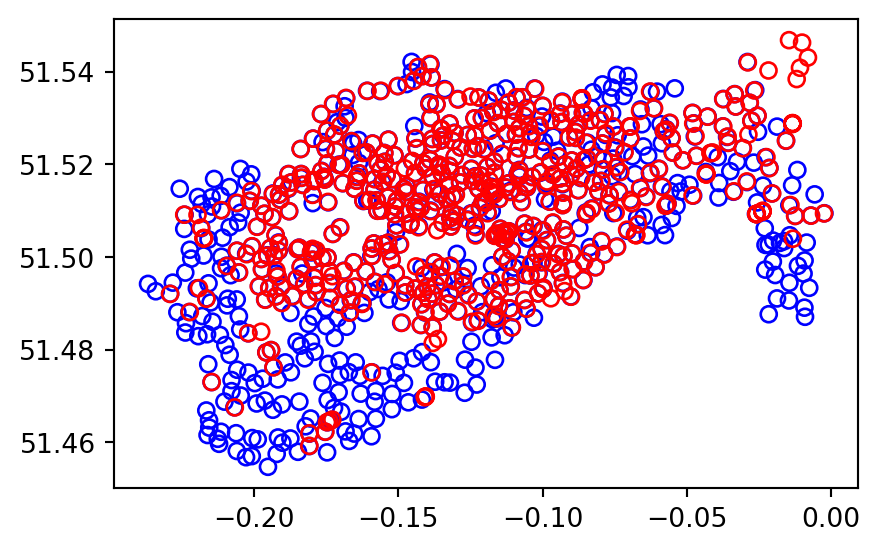
\includegraphics{03-spatial-operations_files/figure-pdf/fig-cycle-hire-output-1.pdf}

}

\caption{\label{fig-cycle-hire}The spatial distribution of cycle hire
points in London based on official data (blue) and OpenStreetMap data
(red).}

\end{figure}%

We can check if any of the points are the same by creating a pairwise
boolean matrix of \texttt{.intersects} relations, then evaluating
whether any of the values in it is \texttt{True}. Note that the
\texttt{.to\_numpy} method is applied to go from a \texttt{DataFrame} to
an \texttt{ndarray}, for which \texttt{.any} gives a global rather than
a row-wise summary. This is what we want in this case, because we are
interested in whether any of the points intersect, not whether any of
the points in each row intersect.

\begin{Shaded}
\begin{Highlighting}[]
\NormalTok{m }\OperatorTok{=}\NormalTok{ cycle\_hire.geometry.}\BuiltInTok{apply}\NormalTok{(}
  \KeywordTok{lambda}\NormalTok{ x: cycle\_hire\_osm.geometry.intersects(x)}
\NormalTok{)}
\NormalTok{m.to\_numpy().}\BuiltInTok{any}\NormalTok{()}
\end{Highlighting}
\end{Shaded}

\begin{verbatim}
np.False_
\end{verbatim}

Imagine that we need to join the capacity variable in
\texttt{cycle\_hire\_osm}
(\texttt{\textquotesingle{}capacity\textquotesingle{}}) onto the
official `target' data contained in \texttt{cycle\_hire}, which looks as
follows.

\begin{Shaded}
\begin{Highlighting}[]
\NormalTok{cycle\_hire}
\end{Highlighting}
\end{Shaded}

\begin{longtable}[]{@{}llllll@{}}
\toprule\noalign{}
& id & name & ... & nempty & geometry \\
\midrule\noalign{}
\endhead
\bottomrule\noalign{}
\endlastfoot
0 & 1 & River Street & ... & 14 & POINT (-0.10997 51.52916) \\
1 & 2 & Phillimore Gardens & ... & 34 & POINT (-0.19757 51.49961) \\
2 & 3 & Christopher Street & ... & 32 & POINT (-0.08461 51.52128) \\
... & ... & ... & ... & ... & ... \\
739 & 775 & Little Brook Green & ... & 17 & POINT (-0.22387 51.49666) \\
740 & 776 & Abyssinia Close & ... & 10 & POINT (-0.16703 51.46033) \\
741 & 777 & Limburg Road & ... & 11 & POINT (-0.1653 51.46192) \\
\end{longtable}

This is when a non-overlapping join is needed. Spatial join
(\texttt{gpd.sjoin}) along with buffered geometries (see
Section~\ref{sec-buffers}) can be used to do that, as demonstrated below
using a threshold distance of 20 \(m\). Note that we transform the data
to a projected CRS (\texttt{27700}) to use real buffer distances, in
meters (see
Section~\ref{sec-geometry-operations-on-projected-and-unprojected-data}).

\begin{Shaded}
\begin{Highlighting}[]
\NormalTok{crs }\OperatorTok{=} \DecValTok{27700}
\NormalTok{cycle\_hire\_buffers }\OperatorTok{=}\NormalTok{ cycle\_hire.copy().to\_crs(crs)}
\NormalTok{cycle\_hire\_buffers.geometry }\OperatorTok{=}\NormalTok{ cycle\_hire\_buffers.}\BuiltInTok{buffer}\NormalTok{(}\DecValTok{20}\NormalTok{)}
\NormalTok{cycle\_hire\_buffers }\OperatorTok{=}\NormalTok{ gpd.sjoin(}
\NormalTok{    cycle\_hire\_buffers, }
\NormalTok{    cycle\_hire\_osm.to\_crs(crs), }
\NormalTok{    how}\OperatorTok{=}\StringTok{\textquotesingle{}left\textquotesingle{}}
\NormalTok{)}
\NormalTok{cycle\_hire\_buffers}
\end{Highlighting}
\end{Shaded}

\begin{longtable}[]{@{}llllll@{}}
\toprule\noalign{}
& id & name\_left & ... & cyclestreets\_id & description \\
\midrule\noalign{}
\endhead
\bottomrule\noalign{}
\endlastfoot
0 & 1 & River Street & ... & None & None \\
1 & 2 & Phillimore Gardens & ... & None & None \\
2 & 3 & Christopher Street & ... & None & None \\
... & ... & ... & ... & ... & ... \\
739 & 775 & Little Brook Green & ... & NaN & NaN \\
740 & 776 & Abyssinia Close & ... & NaN & NaN \\
741 & 777 & Limburg Road & ... & NaN & NaN \\
\end{longtable}

Note that the number of rows in the joined result is greater than the
target. This is because some cycle hire stations in
\texttt{cycle\_hire\_buffers} have multiple matches in
\texttt{cycle\_hire\_osm}. To aggregate the values for the overlapping
points and return the mean, we can use the aggregation methods shown in
Section~\ref{sec-vector-attribute-aggregation}, resulting in an object
with the same number of rows as the target. We also go back from buffers
to points using \texttt{.centroid} method.

\begin{Shaded}
\begin{Highlighting}[]
\NormalTok{cycle\_hire\_buffers }\OperatorTok{=}\NormalTok{ cycle\_hire\_buffers[[}\StringTok{\textquotesingle{}id\textquotesingle{}}\NormalTok{, }\StringTok{\textquotesingle{}capacity\textquotesingle{}}\NormalTok{, }\StringTok{\textquotesingle{}geometry\textquotesingle{}}\NormalTok{]] }\OperatorTok{\textbackslash{}}
\NormalTok{    .dissolve(by}\OperatorTok{=}\StringTok{\textquotesingle{}id\textquotesingle{}}\NormalTok{, aggfunc}\OperatorTok{=}\StringTok{\textquotesingle{}mean\textquotesingle{}}\NormalTok{) }\OperatorTok{\textbackslash{}}
\NormalTok{    .reset\_index()}
\NormalTok{cycle\_hire\_buffers.geometry }\OperatorTok{=}\NormalTok{ cycle\_hire\_buffers.centroid}
\NormalTok{cycle\_hire\_buffers}
\end{Highlighting}
\end{Shaded}

\begin{longtable}[]{@{}llll@{}}
\toprule\noalign{}
& id & geometry & capacity \\
\midrule\noalign{}
\endhead
\bottomrule\noalign{}
\endlastfoot
0 & 1 & POINT (531203.517 182832.066) & 9.0 \\
1 & 2 & POINT (525208.067 179391.922) & 27.0 \\
2 & 3 & POINT (532985.807 182001.572) & NaN \\
... & ... & ... & ... \\
739 & 775 & POINT (523391.016 179020.043) & NaN \\
740 & 776 & POINT (527437.473 175077.168) & NaN \\
741 & 777 & POINT (527553.301 175257) & NaN \\
\end{longtable}

The capacity of nearby stations can be verified by comparing a plot of
the capacity of the source \texttt{cycle\_hire\_osm} data, with the join
results in the new object \texttt{cycle\_hire\_buffers}
(Figure~\ref{fig-cycle-hire-z}).

\begin{Shaded}
\begin{Highlighting}[]
\CommentTok{\# Input}
\NormalTok{fig, ax }\OperatorTok{=}\NormalTok{ plt.subplots(}\DecValTok{1}\NormalTok{, }\DecValTok{1}\NormalTok{, figsize}\OperatorTok{=}\NormalTok{(}\DecValTok{6}\NormalTok{, }\DecValTok{3}\NormalTok{))}
\NormalTok{cycle\_hire\_osm.plot(column}\OperatorTok{=}\StringTok{\textquotesingle{}capacity\textquotesingle{}}\NormalTok{, legend}\OperatorTok{=}\VariableTok{True}\NormalTok{, ax}\OperatorTok{=}\NormalTok{ax)}\OperatorTok{;}
\CommentTok{\# Join result}
\NormalTok{fig, ax }\OperatorTok{=}\NormalTok{ plt.subplots(}\DecValTok{1}\NormalTok{, }\DecValTok{1}\NormalTok{, figsize}\OperatorTok{=}\NormalTok{(}\DecValTok{6}\NormalTok{, }\DecValTok{3}\NormalTok{))}
\NormalTok{cycle\_hire\_buffers.plot(column}\OperatorTok{=}\StringTok{\textquotesingle{}capacity\textquotesingle{}}\NormalTok{, legend}\OperatorTok{=}\VariableTok{True}\NormalTok{, ax}\OperatorTok{=}\NormalTok{ax)}\OperatorTok{;}
\end{Highlighting}
\end{Shaded}

\begin{figure}

\begin{minipage}{0.50\linewidth}

\centering{

\includegraphics{03-spatial-operations_files/figure-pdf/fig-cycle-hire-z-output-1.pdf}

}

\subcaption{\label{fig-cycle-hire-z-1}Input (\texttt{cycle\_hire\_osm})}

\end{minipage}%
%
\begin{minipage}{0.50\linewidth}

\centering{

\includegraphics{03-spatial-operations_files/figure-pdf/fig-cycle-hire-z-output-2.pdf}

}

\subcaption{\label{fig-cycle-hire-z-2}Join result
(\texttt{cycle\_hire\_buffers})}

\end{minipage}%

\caption{\label{fig-cycle-hire-z}Non-overlapping join}

\end{figure}%

\subsection{Spatial aggregation}\label{sec-vector-spatial-aggregation}

As with attribute data aggregation, spatial data aggregation condenses
data: aggregated outputs have fewer rows than non-aggregated inputs.
Statistical aggregating functions, such as mean, average, or sum,
summarize multiple values of a variable, and return a single value per
grouping variable. Section~\ref{sec-vector-attribute-aggregation}
demonstrated how the \texttt{.groupby} method, combined with summary
functions such as \texttt{.sum}, condense data based on attribute
variables. This section shows how grouping by spatial objects can be
achieved using spatial joins combined with non-spatial aggregation.

Returning to the example of New Zealand, imagine you want to find out
the average height of \texttt{nz\_height} points in each region. It is
the geometry of the source (\texttt{nz}) that defines how values in the
target object (\texttt{nz\_height}) are grouped. This can be done in
three steps:

\begin{enumerate}
\def\labelenumi{\arabic{enumi}.}
\tightlist
\item
  Figuring out which \texttt{nz} region each \texttt{nz\_height} point
  falls in---using \texttt{gpd.sjoin}
\item
  Summarizing the average elevation per region---using \texttt{.groupby}
  and \texttt{.mean}
\item
  Joining the result back to \texttt{nz}---using \texttt{pd.merge}
\end{enumerate}

First, we `attach' the region classification of each point, using
spatial join (Section~\ref{sec-spatial-joining}). Note that we are using
the minimal set of columns required: the geometries (for the spatial
join to work), the point elevation (to later calculate an average), and
the region name (to use as key when joining the results back to
\texttt{nz}). The result tells us which \texttt{nz} region each
elevation point falls in.

\begin{Shaded}
\begin{Highlighting}[]
\NormalTok{nz\_height2 }\OperatorTok{=}\NormalTok{ gpd.sjoin(}
\NormalTok{  nz\_height[[}\StringTok{\textquotesingle{}elevation\textquotesingle{}}\NormalTok{, }\StringTok{\textquotesingle{}geometry\textquotesingle{}}\NormalTok{]], }
\NormalTok{  nz[[}\StringTok{\textquotesingle{}Name\textquotesingle{}}\NormalTok{, }\StringTok{\textquotesingle{}geometry\textquotesingle{}}\NormalTok{]], }
\NormalTok{  how}\OperatorTok{=}\StringTok{\textquotesingle{}left\textquotesingle{}}
\NormalTok{)}
\NormalTok{nz\_height2}
\end{Highlighting}
\end{Shaded}

\begin{longtable}[]{@{}lllll@{}}
\toprule\noalign{}
& elevation & geometry & index\_right & Name \\
\midrule\noalign{}
\endhead
\bottomrule\noalign{}
\endlastfoot
0 & 2723 & POINT (1204142.603 5049971.287) & 12 & Southland \\
1 & 2820 & POINT (1234725.325 5048309.302) & 11 & Otago \\
2 & 2830 & POINT (1235914.511 5048745.117) & 11 & Otago \\
... & ... & ... & ... & ... \\
98 & 2751 & POINT (1820659.873 5649488.235) & 2 & Waikato \\
99 & 2720 & POINT (1822262.592 5650428.656) & 2 & Waikato \\
100 & 2732 & POINT (1822492.184 5650492.304) & 2 & Waikato \\
\end{longtable}

Second, we calculate the average elevation, using ordinary (non-spatial)
aggregation (Section~\ref{sec-vector-attribute-aggregation}). This
result tells us the average elevation of all \texttt{nz\_height} points
located within each \texttt{nz} region.

\begin{Shaded}
\begin{Highlighting}[]
\NormalTok{nz\_height2 }\OperatorTok{=}\NormalTok{ nz\_height2.groupby(}\StringTok{\textquotesingle{}Name\textquotesingle{}}\NormalTok{)[[}\StringTok{\textquotesingle{}elevation\textquotesingle{}}\NormalTok{]].mean().reset\_index()}
\NormalTok{nz\_height2}
\end{Highlighting}
\end{Shaded}

\begin{longtable}[]{@{}lll@{}}
\toprule\noalign{}
& Name & elevation \\
\midrule\noalign{}
\endhead
\bottomrule\noalign{}
\endlastfoot
0 & Canterbury & 2994.600000 \\
1 & Manawatu-Wanganui & 2777.000000 \\
2 & Marlborough & 2720.000000 \\
... & ... & ... \\
4 & Southland & 2723.000000 \\
5 & Waikato & 2734.333333 \\
6 & West Coast & 2889.454545 \\
\end{longtable}

The third and final step is joining the averages back to the \texttt{nz}
layer.

\begin{Shaded}
\begin{Highlighting}[]
\NormalTok{nz2 }\OperatorTok{=}\NormalTok{ pd.merge(nz[[}\StringTok{\textquotesingle{}Name\textquotesingle{}}\NormalTok{, }\StringTok{\textquotesingle{}geometry\textquotesingle{}}\NormalTok{]], nz\_height2, on}\OperatorTok{=}\StringTok{\textquotesingle{}Name\textquotesingle{}}\NormalTok{, how}\OperatorTok{=}\StringTok{\textquotesingle{}left\textquotesingle{}}\NormalTok{)}
\NormalTok{nz2}
\end{Highlighting}
\end{Shaded}

\begin{longtable}[]{@{}llll@{}}
\toprule\noalign{}
& Name & geometry & elevation \\
\midrule\noalign{}
\endhead
\bottomrule\noalign{}
\endlastfoot
0 & Northland & MULTIPOLYGON (((1745493.196 600... & NaN \\
1 & Auckland & MULTIPOLYGON (((1803822.103 590... & NaN \\
2 & Waikato & MULTIPOLYGON (((1860345.005 585... & 2734.333333 \\
... & ... & ... & ... \\
13 & Tasman & MULTIPOLYGON (((1616642.877 542... & NaN \\
14 & Nelson & MULTIPOLYGON (((1624866.278 541... & NaN \\
15 & Marlborough & MULTIPOLYGON (((1686901.914 535... & 2720.000000 \\
\end{longtable}

We now have created the \texttt{nz2} layer, which gives the average
\texttt{nz\_height} elevation value per polygon. The result is shown in
Figure~\ref{fig-nz-avg-nz-height}. Note that the \texttt{missing\_kwds}
part determines the style of geometries where the symbology attribute
(\texttt{elevation}) is missing, because there were no
\texttt{nz\_height} points overlapping with them. The default is to omit
them, which is usually not what we want, but with
\texttt{\{\textquotesingle{}color\textquotesingle{}:\textquotesingle{}grey\textquotesingle{},\textquotesingle{}edgecolor\textquotesingle{}:\textquotesingle{}black\textquotesingle{}\}},
those polygons are shown with black outline and grey fill.

\begin{Shaded}
\begin{Highlighting}[]
\NormalTok{nz2.plot(}
\NormalTok{  column}\OperatorTok{=}\StringTok{\textquotesingle{}elevation\textquotesingle{}}\NormalTok{, }
\NormalTok{  legend}\OperatorTok{=}\VariableTok{True}\NormalTok{,}
\NormalTok{  cmap}\OperatorTok{=}\StringTok{\textquotesingle{}Blues\textquotesingle{}}\NormalTok{, edgecolor}\OperatorTok{=}\StringTok{\textquotesingle{}black\textquotesingle{}}\NormalTok{,}
\NormalTok{  missing\_kwds}\OperatorTok{=}\NormalTok{\{}\StringTok{\textquotesingle{}color\textquotesingle{}}\NormalTok{: }\StringTok{\textquotesingle{}grey\textquotesingle{}}\NormalTok{, }\StringTok{\textquotesingle{}edgecolor\textquotesingle{}}\NormalTok{: }\StringTok{\textquotesingle{}black\textquotesingle{}}\NormalTok{\}}
\NormalTok{)}\OperatorTok{;}
\end{Highlighting}
\end{Shaded}

\begin{figure}[H]

\centering{

\includegraphics{03-spatial-operations_files/figure-pdf/fig-nz-avg-nz-height-output-1.pdf}

}

\caption{\label{fig-nz-avg-nz-height}Average height of the top 101 high
points across the regions of New Zealand}

\end{figure}%

\subsection{Joining incongruent
layers}\label{sec-joining-incongruent-layers}

Spatial congruence is an important concept related to spatial
aggregation. An aggregating object (which we will refer to as
\texttt{y}) is congruent with the target object (\texttt{x}) if the two
objects have shared borders. Often this is the case for administrative
boundary data, whereby larger units---such as Middle Layer Super Output
Areas (MSOAs) in the UK, or districts in many other European
countries---are composed of many smaller units.

Incongruent aggregating objects, by contrast, do not share common
borders with the target (Qiu, Zhang, and Zhou 2012). This is problematic
for spatial aggregation (and other spatial operations) illustrated in
Figure~\ref{fig-nz-and-grid}: aggregating the centroid of each sub-zone
will not return accurate results. Areal interpolation overcomes this
issue by transferring values from one set of areal units to another,
using a range of algorithms including simple area-weighted approaches
and more sophisticated approaches such as `pycnophylactic' methods
(Tobler 1979).

To demonstrate joining incongruent layers, we will create a `synthetic'
layer comprising a regular grid of rectangles of size \(100\times100\)
\(km\), covering the extent of the \texttt{nz} layer. This recipe can be
used to create a regular grid covering any given layer (other than
\texttt{nz}), at the specified resolution (\texttt{res}). Most of the
functions have been explained in previous chapters; we leave it as an
exercise for the reader to explore how the code works.

\begin{Shaded}
\begin{Highlighting}[]
\CommentTok{\# Settings: grid extent, resolution, and CRS}
\NormalTok{bounds }\OperatorTok{=}\NormalTok{ nz.total\_bounds}
\NormalTok{crs }\OperatorTok{=}\NormalTok{ nz.crs}
\NormalTok{res }\OperatorTok{=} \DecValTok{100000}
\CommentTok{\# Calculating grid dimensions}
\NormalTok{xmin, ymin, xmax, ymax }\OperatorTok{=}\NormalTok{ bounds}
\NormalTok{cols }\OperatorTok{=} \BuiltInTok{list}\NormalTok{(}\BuiltInTok{range}\NormalTok{(}\BuiltInTok{int}\NormalTok{(np.floor(xmin)), }\BuiltInTok{int}\NormalTok{(np.ceil(xmax}\OperatorTok{+}\NormalTok{res)), res))}
\NormalTok{rows }\OperatorTok{=} \BuiltInTok{list}\NormalTok{(}\BuiltInTok{range}\NormalTok{(}\BuiltInTok{int}\NormalTok{(np.floor(ymin)), }\BuiltInTok{int}\NormalTok{(np.ceil(ymax}\OperatorTok{+}\NormalTok{res)), res))}
\NormalTok{rows.reverse()}
\CommentTok{\# For each cell, create \textquotesingle{}shapely\textquotesingle{} polygon (rectangle)}
\NormalTok{polygons }\OperatorTok{=}\NormalTok{ []}
\ControlFlowTok{for}\NormalTok{ x }\KeywordTok{in}\NormalTok{ cols:}
    \ControlFlowTok{for}\NormalTok{ y }\KeywordTok{in}\NormalTok{ rows:}
\NormalTok{        polygons.append(}
\NormalTok{            shapely.Polygon([(x,y), (x}\OperatorTok{+}\NormalTok{res, y), (x}\OperatorTok{+}\NormalTok{res, y}\OperatorTok{{-}}\NormalTok{res), (x, y}\OperatorTok{{-}}\NormalTok{res)])}
\NormalTok{        )}
\CommentTok{\# To \textquotesingle{}GeoDataFrame\textquotesingle{}}
\NormalTok{grid }\OperatorTok{=}\NormalTok{ gpd.GeoDataFrame(\{}\StringTok{\textquotesingle{}geometry\textquotesingle{}}\NormalTok{: polygons\}, crs}\OperatorTok{=}\NormalTok{crs)}
\CommentTok{\# Remove rows/columns beyond the extent}
\NormalTok{sel }\OperatorTok{=}\NormalTok{ grid.intersects(shapely.box(}\OperatorTok{*}\NormalTok{bounds))}
\NormalTok{grid }\OperatorTok{=}\NormalTok{ grid[sel]}
\CommentTok{\# Add consecultive IDs}
\NormalTok{grid[}\StringTok{\textquotesingle{}id\textquotesingle{}}\NormalTok{] }\OperatorTok{=}\NormalTok{ grid.index}
\NormalTok{grid}
\end{Highlighting}
\end{Shaded}

\begin{longtable}[]{@{}lll@{}}
\toprule\noalign{}
& geometry & id \\
\midrule\noalign{}
\endhead
\bottomrule\noalign{}
\endlastfoot
0 & POLYGON ((1090143 6248536, 1190... & 0 \\
1 & POLYGON ((1090143 6148536, 1190... & 1 \\
2 & POLYGON ((1090143 6048536, 1190... & 2 \\
... & ... & ... \\
156 & POLYGON ((1990143 5048536, 2090... & 156 \\
157 & POLYGON ((1990143 4948536, 2090... & 157 \\
158 & POLYGON ((1990143 4848536, 2090... & 158 \\
\end{longtable}

Figure~\ref{fig-nz-and-grid} shows the newly created \texttt{grid}
layer, along with the \texttt{nz} layer.

\begin{Shaded}
\begin{Highlighting}[]
\NormalTok{base }\OperatorTok{=}\NormalTok{ grid.plot(color}\OperatorTok{=}\StringTok{\textquotesingle{}none\textquotesingle{}}\NormalTok{, edgecolor}\OperatorTok{=}\StringTok{\textquotesingle{}grey\textquotesingle{}}\NormalTok{)}
\NormalTok{nz.plot(}
\NormalTok{    ax}\OperatorTok{=}\NormalTok{base, }
\NormalTok{    column}\OperatorTok{=}\StringTok{\textquotesingle{}Population\textquotesingle{}}\NormalTok{, }
\NormalTok{    edgecolor}\OperatorTok{=}\StringTok{\textquotesingle{}black\textquotesingle{}}\NormalTok{, }
\NormalTok{    legend}\OperatorTok{=}\VariableTok{True}\NormalTok{, }
\NormalTok{    cmap}\OperatorTok{=}\StringTok{\textquotesingle{}Reds\textquotesingle{}}
\NormalTok{)}\OperatorTok{;}
\end{Highlighting}
\end{Shaded}

\begin{figure}[H]

\centering{

\includegraphics{03-spatial-operations_files/figure-pdf/fig-nz-and-grid-output-1.pdf}

}

\caption{\label{fig-nz-and-grid}The \texttt{nz} layer, with population
size in each region, overlaid with a regular \texttt{grid} of
rectangles}

\end{figure}%

Our goal, now, is to `transfer' the
\texttt{\textquotesingle{}Population\textquotesingle{}} attribute
(Figure~\ref{fig-nz-and-grid}) to the rectangular grid polygons, which
is an example of a join between incongruent layers. To do that, we
basically need to calculate---for each \texttt{grid} cell---the weighted
sum of the population in \texttt{nz} polygons coinciding with that cell.
The weights in the weighted sum calculation are the ratios between the
area of the coinciding `part' out of the entire \texttt{nz} polygon.
That is, we (inevitably) assume that the population in each \texttt{nz}
polygon is equally distributed across space, therefore a partial
\texttt{nz} polygon contains the respective partial population size.

We start by calculating the entire area of each \texttt{nz} polygon, as
follows, using the \texttt{.area} method
(Section~\ref{sec-area-length}).

\begin{Shaded}
\begin{Highlighting}[]
\NormalTok{nz[}\StringTok{\textquotesingle{}area\textquotesingle{}}\NormalTok{] }\OperatorTok{=}\NormalTok{ nz.area}
\NormalTok{nz}
\end{Highlighting}
\end{Shaded}

\begin{longtable}[]{@{}llllll@{}}
\toprule\noalign{}
& Name & Island & ... & geometry & area \\
\midrule\noalign{}
\endhead
\bottomrule\noalign{}
\endlastfoot
0 & Northland & North & ... & MULTIPOLYGON (((1745493.196 600... &
1.289058e+10 \\
1 & Auckland & North & ... & MULTIPOLYGON (((1803822.103 590... &
4.911565e+09 \\
2 & Waikato & North & ... & MULTIPOLYGON (((1860345.005 585... &
2.458882e+10 \\
... & ... & ... & ... & ... & ... \\
13 & Tasman & South & ... & MULTIPOLYGON (((1616642.877 542... &
9.594918e+09 \\
14 & Nelson & South & ... & MULTIPOLYGON (((1624866.278 541... &
4.080754e+08 \\
15 & Marlborough & South & ... & MULTIPOLYGON (((1686901.914 535... &
1.046485e+10 \\
\end{longtable}

Next, we use the \texttt{.overlay} method to calculate the pairwise
intersections between \texttt{nz} and \texttt{grid}. As a result, we now
have a layer where each \texttt{nz} polygon is split according to the
\texttt{grid} polygons, hereby named \texttt{nz\_grid}.

\begin{Shaded}
\begin{Highlighting}[]
\NormalTok{nz\_grid }\OperatorTok{=}\NormalTok{ nz.overlay(grid)}
\NormalTok{nz\_grid }\OperatorTok{=}\NormalTok{ nz\_grid[[}\StringTok{\textquotesingle{}id\textquotesingle{}}\NormalTok{, }\StringTok{\textquotesingle{}area\textquotesingle{}}\NormalTok{, }\StringTok{\textquotesingle{}Population\textquotesingle{}}\NormalTok{, }\StringTok{\textquotesingle{}geometry\textquotesingle{}}\NormalTok{]]}
\NormalTok{nz\_grid}
\end{Highlighting}
\end{Shaded}

\begin{longtable}[]{@{}lllll@{}}
\toprule\noalign{}
& id & area & Population & geometry \\
\midrule\noalign{}
\endhead
\bottomrule\noalign{}
\endlastfoot
0 & 64 & 1.289058e+10 & 175500.0 & POLYGON ((1586362.965 6168009.0... \\
1 & 80 & 1.289058e+10 & 175500.0 & POLYGON ((1590143 6162776.641, ... \\
2 & 81 & 1.289058e+10 & 175500.0 & POLYGON ((1633099.964 6066188.0... \\
... & ... & ... & ... & ... \\
107 & 89 & 1.046485e+10 & 46200.0 & POLYGON ((1641283.955
5341361.1... \\
108 & 103 & 1.046485e+10 & 46200.0 & POLYGON ((1690724.332
5458875.4... \\
109 & 104 & 1.046485e+10 & 46200.0 & MULTIPOLYGON (((1694233.995
543... \\
\end{longtable}

Figure~\ref{fig-nz-and-grid-overlay} illustrates the effect of
\texttt{.overlay}:

\begin{Shaded}
\begin{Highlighting}[]
\NormalTok{nz\_grid.plot(color}\OperatorTok{=}\StringTok{\textquotesingle{}none\textquotesingle{}}\NormalTok{, edgecolor}\OperatorTok{=}\StringTok{\textquotesingle{}black\textquotesingle{}}\NormalTok{)}\OperatorTok{;}
\end{Highlighting}
\end{Shaded}

\begin{figure}[H]

\centering{

\includegraphics{03-spatial-operations_files/figure-pdf/fig-nz-and-grid-overlay-output-1.pdf}

}

\caption{\label{fig-nz-and-grid-overlay}The pairwise intersections of
\texttt{nz} and \texttt{grid}, calculated with \texttt{.overlay}}

\end{figure}%

We also need to calculate the areas of the intersections, here into a
new attribute \texttt{\textquotesingle{}area\_sub\textquotesingle{}}. If
an \texttt{nz} polygon was completely within a single \texttt{grid}
polygon, then \texttt{area\_sub} is going to be equal to \texttt{area};
otherwise, it is going to be smaller.

\begin{Shaded}
\begin{Highlighting}[]
\NormalTok{nz\_grid[}\StringTok{\textquotesingle{}area\_sub\textquotesingle{}}\NormalTok{] }\OperatorTok{=}\NormalTok{ nz\_grid.area}
\NormalTok{nz\_grid}
\end{Highlighting}
\end{Shaded}

\begin{longtable}[]{@{}llllll@{}}
\toprule\noalign{}
& id & area & Population & geometry & area\_sub \\
\midrule\noalign{}
\endhead
\bottomrule\noalign{}
\endlastfoot
0 & 64 & 1.289058e+10 & 175500.0 & POLYGON ((1586362.965 6168009.0... &
3.231015e+08 \\
1 & 80 & 1.289058e+10 & 175500.0 & POLYGON ((1590143 6162776.641, ... &
4.612641e+08 \\
2 & 81 & 1.289058e+10 & 175500.0 & POLYGON ((1633099.964 6066188.0... &
5.685656e+09 \\
... & ... & ... & ... & ... & ... \\
107 & 89 & 1.046485e+10 & 46200.0 & POLYGON ((1641283.955 5341361.1... &
1.826943e+09 \\
108 & 103 & 1.046485e+10 & 46200.0 & POLYGON ((1690724.332 5458875.4...
& 1.227037e+08 \\
109 & 104 & 1.046485e+10 & 46200.0 & MULTIPOLYGON (((1694233.995 543...
& 4.874611e+08 \\
\end{longtable}

The resulting layer \texttt{nz\_grid}, with the \texttt{area\_sub}
attribute, is shown in Figure~\ref{fig-nz-and-grid2}.

\begin{Shaded}
\begin{Highlighting}[]
\NormalTok{base }\OperatorTok{=}\NormalTok{ grid.plot(color}\OperatorTok{=}\StringTok{\textquotesingle{}none\textquotesingle{}}\NormalTok{, edgecolor}\OperatorTok{=}\StringTok{\textquotesingle{}grey\textquotesingle{}}\NormalTok{)}
\NormalTok{nz\_grid.plot(}
\NormalTok{    ax}\OperatorTok{=}\NormalTok{base, }
\NormalTok{    column}\OperatorTok{=}\StringTok{\textquotesingle{}area\_sub\textquotesingle{}}\NormalTok{, }
\NormalTok{    edgecolor}\OperatorTok{=}\StringTok{\textquotesingle{}black\textquotesingle{}}\NormalTok{,}
\NormalTok{    legend}\OperatorTok{=}\VariableTok{True}\NormalTok{, }
\NormalTok{    cmap}\OperatorTok{=}\StringTok{\textquotesingle{}Reds\textquotesingle{}}
\NormalTok{)}\OperatorTok{;}
\end{Highlighting}
\end{Shaded}

\begin{figure}[H]

\centering{

\includegraphics{03-spatial-operations_files/figure-pdf/fig-nz-and-grid2-output-1.pdf}

}

\caption{\label{fig-nz-and-grid2}The areas of pairwise intersections in
the \texttt{nz\_grid} layer}

\end{figure}%

Note that each of the intersections still holds the \texttt{Population}
attribute of its `origin' feature of \texttt{nz}, i.e., each portion of
the \texttt{nz} area is associated with the original complete population
count for that area. The real population size of each \texttt{nz\_grid}
feature, however, is smaller, or equal, depending on the geographic area
proportion that it occupies out of the original \texttt{nz} feature. To
make the correction, we first calculate the ratio (\texttt{area\_prop})
and then multiply it by the population. The new (lowercase) attribute
\texttt{population} now has the correct estimate of population sizes in
\texttt{nz\_grid}:

\begin{Shaded}
\begin{Highlighting}[]
\NormalTok{nz\_grid[}\StringTok{\textquotesingle{}area\_prop\textquotesingle{}}\NormalTok{] }\OperatorTok{=}\NormalTok{ nz\_grid[}\StringTok{\textquotesingle{}area\_sub\textquotesingle{}}\NormalTok{] }\OperatorTok{/}\NormalTok{ nz\_grid[}\StringTok{\textquotesingle{}area\textquotesingle{}}\NormalTok{]}
\NormalTok{nz\_grid[}\StringTok{\textquotesingle{}population\textquotesingle{}}\NormalTok{] }\OperatorTok{=}\NormalTok{ nz\_grid[}\StringTok{\textquotesingle{}Population\textquotesingle{}}\NormalTok{] }\OperatorTok{*}\NormalTok{ nz\_grid[}\StringTok{\textquotesingle{}area\_prop\textquotesingle{}}\NormalTok{]}
\NormalTok{nz\_grid}
\end{Highlighting}
\end{Shaded}

\begin{longtable}[]{@{}llllll@{}}
\toprule\noalign{}
& id & area & ... & area\_prop & population \\
\midrule\noalign{}
\endhead
\bottomrule\noalign{}
\endlastfoot
0 & 64 & 1.289058e+10 & ... & 0.025065 & 4398.897141 \\
1 & 80 & 1.289058e+10 & ... & 0.035783 & 6279.925114 \\
2 & 81 & 1.289058e+10 & ... & 0.441071 & 77407.916241 \\
... & ... & ... & ... & ... & ... \\
107 & 89 & 1.046485e+10 & ... & 0.174579 & 8065.550415 \\
108 & 103 & 1.046485e+10 & ... & 0.011725 & 541.709946 \\
109 & 104 & 1.046485e+10 & ... & 0.046581 & 2152.033881 \\
\end{longtable}

What is left to be done is to sum (see
Section~\ref{sec-vector-attribute-aggregation}) the population in all
parts forming the same grid cell and join (see
Section~\ref{sec-vector-attribute-joining}) them back to the
\texttt{grid} layer. Note that many of the grid cells have `No Data' for
population, because they have no intersection with \texttt{nz} at all
(Figure~\ref{fig-nz-and-grid}).

\begin{Shaded}
\begin{Highlighting}[]
\NormalTok{nz\_grid }\OperatorTok{=}\NormalTok{ nz\_grid.groupby(}\StringTok{\textquotesingle{}id\textquotesingle{}}\NormalTok{)[}\StringTok{\textquotesingle{}population\textquotesingle{}}\NormalTok{].}\BuiltInTok{sum}\NormalTok{().reset\_index()}
\NormalTok{grid }\OperatorTok{=}\NormalTok{ pd.merge(grid, nz\_grid[[}\StringTok{\textquotesingle{}id\textquotesingle{}}\NormalTok{, }\StringTok{\textquotesingle{}population\textquotesingle{}}\NormalTok{]], on}\OperatorTok{=}\StringTok{\textquotesingle{}id\textquotesingle{}}\NormalTok{, how}\OperatorTok{=}\StringTok{\textquotesingle{}left\textquotesingle{}}\NormalTok{)}
\NormalTok{grid}
\end{Highlighting}
\end{Shaded}

\begin{longtable}[]{@{}llll@{}}
\toprule\noalign{}
& geometry & id & population \\
\midrule\noalign{}
\endhead
\bottomrule\noalign{}
\endlastfoot
0 & POLYGON ((1090143 6248536, 1190... & 0 & NaN \\
1 & POLYGON ((1090143 6148536, 1190... & 1 & NaN \\
2 & POLYGON ((1090143 6048536, 1190... & 2 & NaN \\
... & ... & ... & ... \\
147 & POLYGON ((1990143 5048536, 2090... & 156 & NaN \\
148 & POLYGON ((1990143 4948536, 2090... & 157 & NaN \\
149 & POLYGON ((1990143 4848536, 2090... & 158 & NaN \\
\end{longtable}

Figure~\ref{fig-nz-and-grid3} shows the final result \texttt{grid} with
the incongruently-joined \texttt{population} attribute from \texttt{nz}.

\begin{Shaded}
\begin{Highlighting}[]
\NormalTok{base }\OperatorTok{=}\NormalTok{ grid.plot(}
\NormalTok{    column}\OperatorTok{=}\StringTok{\textquotesingle{}population\textquotesingle{}}\NormalTok{, }
\NormalTok{    edgecolor}\OperatorTok{=}\StringTok{\textquotesingle{}black\textquotesingle{}}\NormalTok{,}
\NormalTok{    legend}\OperatorTok{=}\VariableTok{True}\NormalTok{, }
\NormalTok{    cmap}\OperatorTok{=}\StringTok{\textquotesingle{}Reds\textquotesingle{}}
\NormalTok{)}\OperatorTok{;}
\NormalTok{nz.plot(ax}\OperatorTok{=}\NormalTok{base, color}\OperatorTok{=}\StringTok{\textquotesingle{}none\textquotesingle{}}\NormalTok{, edgecolor}\OperatorTok{=}\StringTok{\textquotesingle{}grey\textquotesingle{}}\NormalTok{, legend}\OperatorTok{=}\VariableTok{True}\NormalTok{)}\OperatorTok{;}
\end{Highlighting}
\end{Shaded}

\begin{figure}[H]

\centering{

\includegraphics{03-spatial-operations_files/figure-pdf/fig-nz-and-grid3-output-1.pdf}

}

\caption{\label{fig-nz-and-grid3}The \texttt{nz} layer and a regular
grid of rectangles: final result}

\end{figure}%

We can demonstrate that, expectedly, the summed population in
\texttt{nz} and \texttt{grid} is identical, even though the geometry is
different (since we created \texttt{grid} to completely cover
\texttt{nz}), by comparing the \texttt{.sum} of the \texttt{population}
attribute in both layers.

\begin{Shaded}
\begin{Highlighting}[]
\NormalTok{nz[}\StringTok{\textquotesingle{}Population\textquotesingle{}}\NormalTok{].}\BuiltInTok{sum}\NormalTok{()}
\end{Highlighting}
\end{Shaded}

\begin{verbatim}
np.float64(4787200.0)
\end{verbatim}

\begin{Shaded}
\begin{Highlighting}[]
\NormalTok{grid[}\StringTok{\textquotesingle{}population\textquotesingle{}}\NormalTok{].}\BuiltInTok{sum}\NormalTok{()}
\end{Highlighting}
\end{Shaded}

\begin{verbatim}
np.float64(4787199.999999998)
\end{verbatim}

The procedure in this section is known as an area-weighted interpolation
of a spatially \emph{extensive} (e.g., population) variable. In
extensive interpolation, we assume that the variable of interest
represents counts (such as, here, inhabitants) uniformly distributed
across space. In such case, each part of a given polygon captures the
respective proportion of counts (such as, half of a region with \(N\)
inhabitants contains \(N/2\) inhabitants). Accordingly, summing the
parts gives the total count of the total area.

An area-weighted interpolation of a spatially \emph{intensive} variable
(e.g., population density) is almost identical, except that we would
have to calculate the weighted \texttt{.mean} rather than \texttt{.sum},
to preserve the average rather than the sum. In intensive interpolation,
we assume that the variable of interest represents counts per unit area,
i.e., density. Since density is (assumed to be) uniform, any part of a
given polygon has exactly the same density as that of the whole polygon.
Density values are therefore computed as weighted averages, rather than
sums, of the parts. Also, see the `Area-weighted interpolation' section
in Pebesma and Bivand (2023).

\subsection{Distance relations}\label{sec-distance-relations}

While topological relations are binary---a feature either intersects
with another or does not---distance relations are continuous. The
distance between two objects is calculated with the \texttt{.distance}
method. The method is applied on a \texttt{GeoSeries} (or a
\texttt{GeoDataFrame}), with the argument being an individual
\texttt{shapely} geometry. The result is a \texttt{Series} of pairwise
distances.

\begin{tcolorbox}[enhanced jigsaw, breakable, title=\textcolor{quarto-callout-note-color}{\faInfo}\hspace{0.5em}{Note}, arc=.35mm, opacitybacktitle=0.6, left=2mm, colback=white, bottomrule=.15mm, bottomtitle=1mm, toptitle=1mm, colframe=quarto-callout-note-color-frame, leftrule=.75mm, rightrule=.15mm, toprule=.15mm, titlerule=0mm, opacityback=0, colbacktitle=quarto-callout-note-color!10!white, coltitle=black]

\textbf{geopandas} uses similar syntax and mode of operation for many of
its methods and functions, including:

\begin{itemize}
\tightlist
\item
  Numeric calculations, such as \texttt{.distance} (this section),
  returning numeric values
\item
  Topological evaluation methods, such as \texttt{.intersects} or
  \texttt{.disjoint} (Section~\ref{sec-topological-relations}),
  returning boolean values
\item
  Geometry generating-methods, such as \texttt{.intersection}
  (Section~\ref{sec-clipping}), returning geometries
\end{itemize}

In all cases, the input is a \texttt{GeoSeries} and (or a
\texttt{GeoDataFrame}) and a \texttt{shapely} geometry, and the output
is a \texttt{Series} or \texttt{GeoSeries} of results, contrasting each
geometry from the \texttt{GeoSeries} with the \texttt{shapely} geometry.
The examples in this book demonstrate this, so-called `many-to-one',
mode of the functions.

All of the above-mentioned methods also have a pairwise mode, perhaps
less useful and not used in the book, where we evaluate relations
between pairs of geometries in two \texttt{GeoSeries}, aligned either by
index or by position.

\end{tcolorbox}

To illustrate the \texttt{.distance} method, let's take the three
highest points in New Zealand with \texttt{.sort\_values} and
\texttt{.iloc}.

\begin{Shaded}
\begin{Highlighting}[]
\NormalTok{nz\_highest }\OperatorTok{=}\NormalTok{ nz\_height.sort\_values(by}\OperatorTok{=}\StringTok{\textquotesingle{}elevation\textquotesingle{}}\NormalTok{, ascending}\OperatorTok{=}\VariableTok{False}\NormalTok{).iloc[:}\DecValTok{3}\NormalTok{, :]}
\NormalTok{nz\_highest}
\end{Highlighting}
\end{Shaded}

\begin{longtable}[]{@{}llll@{}}
\toprule\noalign{}
& t50\_fid & elevation & geometry \\
\midrule\noalign{}
\endhead
\bottomrule\noalign{}
\endlastfoot
64 & 2372236 & 3724 & POINT (1369317.63 5169132.284) \\
63 & 2372235 & 3717 & POINT (1369512.866 5168235.616) \\
67 & 2372252 & 3688 & POINT (1369381.942 5168761.875) \\
\end{longtable}

Additionally, we need the geographic centroid of the Canterbury region
(\texttt{canterbury}, created in
Section~\ref{sec-spatial-subsetting-vector}).

\begin{Shaded}
\begin{Highlighting}[]
\NormalTok{canterbury\_centroid }\OperatorTok{=}\NormalTok{ canterbury.centroid.iloc[}\DecValTok{0}\NormalTok{]}
\end{Highlighting}
\end{Shaded}

Now we are able to apply \texttt{.distance} to calculate the distances
from each of the three elevation points to the centroid of the
Canterbury region.

\begin{Shaded}
\begin{Highlighting}[]
\NormalTok{nz\_highest.distance(canterbury\_centroid)}
\end{Highlighting}
\end{Shaded}

\begin{verbatim}
64    115539.995747
63    115390.248038
67    115493.594066
dtype: float64
\end{verbatim}

To obtain a distance matrix, i.e., a pairwise set of distances between
all combinations of features in objects \texttt{x} and \texttt{y}, we
need to use the \texttt{.apply} method (analogous to the way we created
the \texttt{.intersects} boolean matrix in
Section~\ref{sec-topological-relations}). To illustrate this, let's now
take two regions in \texttt{nz}, Otago and Canterbury, represented by
the object \texttt{co}.

\begin{Shaded}
\begin{Highlighting}[]
\NormalTok{sel }\OperatorTok{=}\NormalTok{ nz[}\StringTok{\textquotesingle{}Name\textquotesingle{}}\NormalTok{].}\BuiltInTok{str}\NormalTok{.contains(}\StringTok{\textquotesingle{}Canter|Otag\textquotesingle{}}\NormalTok{)}
\NormalTok{co }\OperatorTok{=}\NormalTok{ nz[sel]}
\NormalTok{co}
\end{Highlighting}
\end{Shaded}

\begin{longtable}[]{@{}llllll@{}}
\toprule\noalign{}
& Name & Island & ... & geometry & area \\
\midrule\noalign{}
\endhead
\bottomrule\noalign{}
\endlastfoot
10 & Canterbury & South & ... & MULTIPOLYGON (((1686901.914 535... &
4.532656e+10 \\
11 & Otago & South & ... & MULTIPOLYGON (((1335204.789 512... &
3.190356e+10 \\
\end{longtable}

The distance matrix (technically speaking, a \texttt{DataFrame})
\texttt{d} between each of the first three elevation points, and the two
regions, is then obtained as follows. In plain language, we take the
geometry from each each row in \texttt{nz\_height.iloc{[}:3,:{]}}, and
apply the \texttt{.distance} method on \texttt{co} with its rows as the
argument.

\begin{Shaded}
\begin{Highlighting}[]
\NormalTok{d }\OperatorTok{=}\NormalTok{ nz\_height.iloc[:}\DecValTok{3}\NormalTok{, :].}\BuiltInTok{apply}\NormalTok{(}\KeywordTok{lambda}\NormalTok{ x: co.distance(x.geometry), axis}\OperatorTok{=}\DecValTok{1}\NormalTok{)}
\NormalTok{d}
\end{Highlighting}
\end{Shaded}

\begin{longtable}[]{@{}lll@{}}
\toprule\noalign{}
& 10 & 11 \\
\midrule\noalign{}
\endhead
\bottomrule\noalign{}
\endlastfoot
0 & 123537.158269 & 15497.717252 \\
1 & 94282.773074 & 0.000000 \\
2 & 93018.560814 & 0.000000 \\
\end{longtable}

Note that the distance between the second and third features in
\texttt{nz\_height} and the second feature in \texttt{co} is zero. This
demonstrates the fact that distances between points and polygons refer
to the distance to any part of the polygon: the second and third points
in \texttt{nz\_height} are in Otago, which can be verified by plotting
them (two almost completely overlappling points in
Figure~\ref{fig-nz-height-and-otago}).

\begin{Shaded}
\begin{Highlighting}[]
\NormalTok{fig, ax }\OperatorTok{=}\NormalTok{ plt.subplots()}
\NormalTok{co.plot(color}\OperatorTok{=}\StringTok{\textquotesingle{}lightgrey\textquotesingle{}}\NormalTok{, edgecolor}\OperatorTok{=}\StringTok{\textquotesingle{}black\textquotesingle{}}\NormalTok{, ax}\OperatorTok{=}\NormalTok{ax)}
\NormalTok{co.}\BuiltInTok{apply}\NormalTok{(}
    \KeywordTok{lambda}\NormalTok{ x: ax.annotate(}
\NormalTok{        text}\OperatorTok{=}\NormalTok{x[}\StringTok{\textquotesingle{}Name\textquotesingle{}}\NormalTok{], }
\NormalTok{        xy}\OperatorTok{=}\NormalTok{x.geometry.centroid.coords[}\DecValTok{0}\NormalTok{], }
\NormalTok{        ha}\OperatorTok{=}\StringTok{\textquotesingle{}center\textquotesingle{}}
\NormalTok{    ), }
\NormalTok{    axis}\OperatorTok{=}\DecValTok{1}
\NormalTok{)}
\NormalTok{nz\_height.iloc[:}\DecValTok{3}\NormalTok{, :].plot(color}\OperatorTok{=}\StringTok{\textquotesingle{}none\textquotesingle{}}\NormalTok{, edgecolor}\OperatorTok{=}\StringTok{\textquotesingle{}black\textquotesingle{}}\NormalTok{, ax}\OperatorTok{=}\NormalTok{ax)}\OperatorTok{;}
\end{Highlighting}
\end{Shaded}

\begin{figure}[H]

\centering{

\includegraphics{03-spatial-operations_files/figure-pdf/fig-nz-height-and-otago-output-1.pdf}

}

\caption{\label{fig-nz-height-and-otago}The first three
\texttt{nz\_height} points, and the Otago and Canterbury regions from
\texttt{nz}}

\end{figure}%

\section{Spatial operations on raster data}\label{sec-spatial-ras}

This section builds on Section~\ref{sec-manipulating-raster-objects},
which highlights various basic methods for manipulating raster datasets,
to demonstrate more advanced and explicitly spatial raster operations,
and uses the \texttt{elev.tif} and \texttt{grain.tif} rasters manually
created in Section~\ref{sec-raster-from-scratch}.

\subsection{Spatial subsetting}\label{sec-spatial-subsetting-raster}

The previous chapter (and especially
Section~\ref{sec-manipulating-raster-objects}) demonstrated how to
retrieve values associated with specific row and column combinations
from a raster. Raster values can also be extracted by location
(coordinates) and other spatial objects. To use coordinates for
subsetting, we can use the \texttt{.sample} method of a
\texttt{rasterio} file connection object, combined with a list of
coordinate tuples. The method is demonstrated below to find the value of
the cell that covers a point located at coordinates of
\texttt{(0.1,0.1)} in \texttt{elev}. The returned object is a
\emph{generator}. The rationale for returning a generator, rather than a
\texttt{list}, is memory efficiency. The number of sampled points may be
huge, in which case we would want to generate the values one at a time
rather than all at once.

\begin{Shaded}
\begin{Highlighting}[]
\NormalTok{src\_elev.sample([(}\FloatTok{0.1}\NormalTok{, }\FloatTok{0.1}\NormalTok{)])}
\end{Highlighting}
\end{Shaded}

\begin{verbatim}
<generator object sample_gen at 0x78ff6f120f40>
\end{verbatim}

\begin{tcolorbox}[enhanced jigsaw, breakable, title=\textcolor{quarto-callout-note-color}{\faInfo}\hspace{0.5em}{Note}, arc=.35mm, opacitybacktitle=0.6, left=2mm, colback=white, bottomrule=.15mm, bottomtitle=1mm, toptitle=1mm, colframe=quarto-callout-note-color-frame, leftrule=.75mm, rightrule=.15mm, toprule=.15mm, titlerule=0mm, opacityback=0, colbacktitle=quarto-callout-note-color!10!white, coltitle=black]

The technical terms \emph{iterable}, \emph{iterator}, and
\emph{generator} in Python may be confusing, so here is a short summary,
ordered from most general to most specific:

\begin{itemize}
\tightlist
\item
  An \emph{iterable} is any object that we can iterate on, such as using
  a \texttt{for} loop. For example, a \texttt{list} is iterable.
\item
  An \emph{iterator} is an object that represents a stream of data,
  which we can go over, each time getting the next element using
  \texttt{next}. Iterators are also iterable, meaning that you can over
  them in a loop, but they are stateful (e.g., they remember which item
  was obtained using \texttt{next}), meaning that you can go over them
  just once.
\item
  A \emph{generator} is a function that returns an iterator. For
  example, the \texttt{.sample} method in the above example is a
  generator. The \textbf{rasterio} package makes use of generators in
  some of its functions, as we will see later on
  (Section~\ref{sec-raster-to-polygons}).
\end{itemize}

\end{tcolorbox}

In case we nevertheless want all values at once, such as when the number
of points is small, we can force the generatrion of all values from a
generator at once, using \texttt{list}. Since there was just one point,
the result is one extracted value, in this case \texttt{16}.

\begin{Shaded}
\begin{Highlighting}[]
\BuiltInTok{list}\NormalTok{(src\_elev.sample([(}\FloatTok{0.1}\NormalTok{, }\FloatTok{0.1}\NormalTok{)]))}
\end{Highlighting}
\end{Shaded}

\begin{verbatim}
[array([16], dtype=uint8)]
\end{verbatim}

We can use the same technique to extract the values of multiple points
at once. For example, here we extract the raster values at two points,
\texttt{(0.1,0.1)} and \texttt{(1.1,1.1)}. The resulting values are
\texttt{16} and \texttt{6}.

\begin{Shaded}
\begin{Highlighting}[]
\BuiltInTok{list}\NormalTok{(src\_elev.sample([(}\FloatTok{0.1}\NormalTok{, }\FloatTok{0.1}\NormalTok{), (}\FloatTok{1.1}\NormalTok{, }\FloatTok{1.1}\NormalTok{)]))}
\end{Highlighting}
\end{Shaded}

\begin{verbatim}
[array([16], dtype=uint8), array([6], dtype=uint8)]
\end{verbatim}

The location of the two sample points on top of the \texttt{elev.tif}
raster is illustrated in Figure~\ref{fig-elev-sample-points}.

\begin{Shaded}
\begin{Highlighting}[]
\NormalTok{fig, ax }\OperatorTok{=}\NormalTok{ plt.subplots()}
\NormalTok{rasterio.plot.show(src\_elev, ax}\OperatorTok{=}\NormalTok{ax)}
\NormalTok{gpd.GeoSeries([shapely.Point(}\FloatTok{0.1}\NormalTok{, }\FloatTok{0.1}\NormalTok{)]) }\OperatorTok{\textbackslash{}}
\NormalTok{    .plot(color}\OperatorTok{=}\StringTok{\textquotesingle{}black\textquotesingle{}}\NormalTok{, edgecolor}\OperatorTok{=}\StringTok{\textquotesingle{}white\textquotesingle{}}\NormalTok{, markersize}\OperatorTok{=}\DecValTok{50}\NormalTok{, ax}\OperatorTok{=}\NormalTok{ax)}
\NormalTok{gpd.GeoSeries([shapely.Point(}\FloatTok{1.1}\NormalTok{, }\FloatTok{1.1}\NormalTok{)]) }\OperatorTok{\textbackslash{}}
\NormalTok{    .plot(color}\OperatorTok{=}\StringTok{\textquotesingle{}black\textquotesingle{}}\NormalTok{, edgecolor}\OperatorTok{=}\StringTok{\textquotesingle{}white\textquotesingle{}}\NormalTok{, markersize}\OperatorTok{=}\DecValTok{50}\NormalTok{, ax}\OperatorTok{=}\NormalTok{ax)}\OperatorTok{;}
\end{Highlighting}
\end{Shaded}

\begin{figure}[H]

\centering{

\includegraphics{03-spatial-operations_files/figure-pdf/fig-elev-sample-points-output-1.pdf}

}

\caption{\label{fig-elev-sample-points}The \texttt{elev.tif} raster, and
two points where we extract its values}

\end{figure}%

\begin{tcolorbox}[enhanced jigsaw, breakable, title=\textcolor{quarto-callout-note-color}{\faInfo}\hspace{0.5em}{Note}, arc=.35mm, opacitybacktitle=0.6, left=2mm, colback=white, bottomrule=.15mm, bottomtitle=1mm, toptitle=1mm, colframe=quarto-callout-note-color-frame, leftrule=.75mm, rightrule=.15mm, toprule=.15mm, titlerule=0mm, opacityback=0, colbacktitle=quarto-callout-note-color!10!white, coltitle=black]

We elaborate on the plotting technique used to display the points and
the raster in Section~\ref{sec-plot-static-layers}. We will also
introduce a more user-friendly and general method to extract raster
values to points, using the \textbf{rasterstats} package, in
Section~\ref{sec-extraction-to-points}.

\end{tcolorbox}

Another common use case of spatial subsetting is using a boolean mask,
based on another raster with the same extent and resolution, or the
original one, as illustrated in Figure~\ref{fig-raster-subset}. To do
that, we erase the values in the array of one raster, according to
another corresponding mask raster. For example, let's read
(Section~\ref{sec-using-rasterio}) the \texttt{elev.tif} raster values
into an array named \texttt{elev} (Figure~\ref{fig-raster-subset} (a)).

\begin{Shaded}
\begin{Highlighting}[]
\NormalTok{elev }\OperatorTok{=}\NormalTok{ src\_elev.read(}\DecValTok{1}\NormalTok{)}
\NormalTok{elev}
\end{Highlighting}
\end{Shaded}

\begin{verbatim}
array([[ 1,  2,  3,  4,  5,  6],
       [ 7,  8,  9, 10, 11, 12],
       [13, 14, 15, 16, 17, 18],
       [19, 20, 21, 22, 23, 24],
       [25, 26, 27, 28, 29, 30],
       [31, 32, 33, 34, 35, 36]], dtype=uint8)
\end{verbatim}

and create a corresponding random boolean mask named \texttt{mask}
(Figure~\ref{fig-raster-subset} (b)), of the same shape as
\texttt{elev.tif} with values randomly assigned to \texttt{True} and
\texttt{False}.

\begin{Shaded}
\begin{Highlighting}[]
\NormalTok{np.random.seed(}\DecValTok{1}\NormalTok{)}
\NormalTok{mask }\OperatorTok{=}\NormalTok{ np.random.choice([}\VariableTok{True}\NormalTok{, }\VariableTok{False}\NormalTok{], src\_elev.shape)}
\NormalTok{mask}
\end{Highlighting}
\end{Shaded}

\begin{verbatim}
array([[False, False,  True,  True, False, False],
       [False, False, False,  True,  True, False],
       [ True, False, False,  True,  True, False],
       [ True,  True,  True, False,  True,  True],
       [False,  True,  True,  True, False,  True],
       [ True,  True, False, False, False, False]])
\end{verbatim}

Next, suppose that we want to keep only those values of \texttt{elev}
which are \texttt{False} in \texttt{mask} (i.e., they are \emph{not}
masked). In other words, we want to mask \texttt{elev} with
\texttt{mask}. The result will be stored in a copy named
\texttt{masked\_elev} (Figure~\ref{fig-raster-subset} (c)). In the case
of \texttt{elev.tif}, to be able to store \texttt{np.nan} in the array
of values, we also need to convert it to \texttt{float} (see
Section~\ref{sec-summarizing-raster-objects}). Afterwards, masking is a
matter of assigning \texttt{np.nan} into a subset defined by the mask,
using the `boolean array indexing' syntax of \textbf{numpy}.

\begin{Shaded}
\begin{Highlighting}[]
\NormalTok{masked\_elev }\OperatorTok{=}\NormalTok{ elev.copy()}
\NormalTok{masked\_elev }\OperatorTok{=}\NormalTok{ masked\_elev.astype(}\StringTok{\textquotesingle{}float64\textquotesingle{}}\NormalTok{)}
\NormalTok{masked\_elev[mask] }\OperatorTok{=}\NormalTok{ np.nan}
\NormalTok{masked\_elev}
\end{Highlighting}
\end{Shaded}

\begin{verbatim}
array([[ 1.,  2., nan, nan,  5.,  6.],
       [ 7.,  8.,  9., nan, nan, 12.],
       [nan, 14., 15., nan, nan, 18.],
       [nan, nan, nan, 22., nan, nan],
       [25., nan, nan, nan, 29., nan],
       [nan, nan, 33., 34., 35., 36.]])
\end{verbatim}

Figure~\ref{fig-raster-subset} shows the original \texttt{elev} raster,
the \texttt{mask} raster, and the resulting \texttt{masked\_elev}
raster.

\begin{Shaded}
\begin{Highlighting}[]
\NormalTok{rasterio.plot.show(elev)}\OperatorTok{;}
\NormalTok{rasterio.plot.show(mask)}\OperatorTok{;}
\NormalTok{rasterio.plot.show(masked\_elev)}\OperatorTok{;}
\end{Highlighting}
\end{Shaded}

\begin{figure}

\begin{minipage}{0.33\linewidth}

\centering{

\includegraphics{03-spatial-operations_files/figure-pdf/fig-raster-subset-output-1.pdf}

}

\subcaption{\label{fig-raster-subset-1}Original raster}

\end{minipage}%
%
\begin{minipage}{0.33\linewidth}

\centering{

\includegraphics{03-spatial-operations_files/figure-pdf/fig-raster-subset-output-2.pdf}

}

\subcaption{\label{fig-raster-subset-2}Raster mask}

\end{minipage}%
%
\begin{minipage}{0.33\linewidth}

\centering{

\includegraphics{03-spatial-operations_files/figure-pdf/fig-raster-subset-output-3.pdf}

}

\subcaption{\label{fig-raster-subset-3}Output masked raster}

\end{minipage}%

\caption{\label{fig-raster-subset}Subsetting raster values using a
boolean mask}

\end{figure}%

The mask can be created from the array itself, using condition(s). That
way, we can replace some values (e.g., values assumed to be wrong) with
\texttt{np.nan}, such as in the following example.

\begin{Shaded}
\begin{Highlighting}[]
\NormalTok{elev2 }\OperatorTok{=}\NormalTok{ elev.copy()}
\NormalTok{elev2 }\OperatorTok{=}\NormalTok{ elev2.astype(}\StringTok{\textquotesingle{}float64\textquotesingle{}}\NormalTok{)}
\NormalTok{elev2[elev2 }\OperatorTok{\textless{}} \DecValTok{20}\NormalTok{] }\OperatorTok{=}\NormalTok{ np.nan}
\NormalTok{elev2}
\end{Highlighting}
\end{Shaded}

\begin{verbatim}
array([[nan, nan, nan, nan, nan, nan],
       [nan, nan, nan, nan, nan, nan],
       [nan, nan, nan, nan, nan, nan],
       [nan, 20., 21., 22., 23., 24.],
       [25., 26., 27., 28., 29., 30.],
       [31., 32., 33., 34., 35., 36.]])
\end{verbatim}

This technique is also used to reclassify raster values (see
Section~\ref{sec-raster-local-operations}).

\subsection{Map algebra}\label{sec-map-algebra}

The term `map algebra' was coined in the late 1970s to describe a `set
of conventions, capabilities, and techniques' for the analysis of
geographic raster and (although less prominently) vector data (Tomlin
1994). In this context, we define map algebra more narrowly, as
operations that modify or summarize raster cell values, with reference
to surrounding cells, zones, or statistical functions that apply to
every cell.

Map algebra operations tend to be fast, because raster datasets only
implicitly store coordinates, hence the old adage `raster is faster but
vector is corrector'. The location of cells in raster datasets can be
calculated by using its matrix position and the resolution and origin of
the dataset (stored in the raster metadata,
Section~\ref{sec-using-rasterio}). For the processing, however, the
geographic position of a cell is barely relevant as long as we make sure
that the cell position is still the same after the processing.
Additionally, if two or more raster datasets share the same extent,
projection, and resolution, one could treat them as matrices for the
processing.

Map algebra (or cartographic modeling with raster data) divides raster
operations into four subclasses (Tomlin 1990), with each working on one
or several grids simultaneously:

\begin{itemize}
\tightlist
\item
  Local or per-cell operations
  (Section~\ref{sec-raster-local-operations})
\item
  Focal or neighborhood operations. Most often the output cell value is
  the result of a \(3 \times 3\) input cell block
  (Section~\ref{sec-focal-operations})
\item
  Zonal operations are similar to focal operations, but the surrounding
  pixel grid on which new values are computed can have irregular sizes
  and shapes (Section~\ref{sec-zonal-operations})
\item
  Global or per-raster operations; that means the output cell derives
  its value potentially from one or several entire rasters
  (Section~\ref{sec-global-operations-and-distances})
\end{itemize}

This typology classifies map algebra operations by the number of cells
used for each pixel processing step and the type of output. For the sake
of completeness, we should mention that raster operations can also be
classified by disciplines such as terrain, hydrological analysis, or
image classification. The following sections explain how each type of
map algebra operations can be used, with reference to worked examples.

\subsection{Local operations}\label{sec-raster-local-operations}

Local operations comprise all cell-by-cell operations in one or several
layers. Raster algebra is a classical use case of local
operations---this includes adding or subtracting values from a raster,
squaring, and multiplying rasters. Raster algebra also allows logical
operations such as finding all raster cells that are greater than a
specific value (e.g., \texttt{5} in our example below). Local operations
are applied using the \textbf{numpy} array operations syntax, as
demonstrated below.

First, let's take the array of \texttt{elev.tif} raster values, which we
already read earlier (Section~\ref{sec-spatial-subsetting-raster}).

\begin{Shaded}
\begin{Highlighting}[]
\NormalTok{elev}
\end{Highlighting}
\end{Shaded}

\begin{verbatim}
array([[ 1,  2,  3,  4,  5,  6],
       [ 7,  8,  9, 10, 11, 12],
       [13, 14, 15, 16, 17, 18],
       [19, 20, 21, 22, 23, 24],
       [25, 26, 27, 28, 29, 30],
       [31, 32, 33, 34, 35, 36]], dtype=uint8)
\end{verbatim}

Now, any element-wise array operation can be applied using
\textbf{numpy} arithmetic or conditional operators and functions,
comprising local raster operations in spatial analysis terminology. For
example, \texttt{elev+elev} adds the values of \texttt{elev} to itself,
resulting in a raster with double values.

\begin{Shaded}
\begin{Highlighting}[]
\NormalTok{elev }\OperatorTok{+}\NormalTok{ elev}
\end{Highlighting}
\end{Shaded}

\begin{verbatim}
array([[ 2,  4,  6,  8, 10, 12],
       [14, 16, 18, 20, 22, 24],
       [26, 28, 30, 32, 34, 36],
       [38, 40, 42, 44, 46, 48],
       [50, 52, 54, 56, 58, 60],
       [62, 64, 66, 68, 70, 72]], dtype=uint8)
\end{verbatim}

Note that some functions and operators automatically change the data
type to accommodate the resulting values, while other operators do not,
potentially resulting in overflow (i.e., incorrect values for results
beyond the data type range, such as trying to accommodate values above
\texttt{255} in an \texttt{int8} array). For example, \texttt{elev**2}
(\texttt{elev} squared) results in overflow. Since the \texttt{**}
operator does not automatically change the data type, leaving it as
\texttt{int8}, the resulting array has incorrect values for
\texttt{16**2}, \texttt{17**2}, etc., which are above \texttt{255} and
therefore cannot be accommodated.

\begin{Shaded}
\begin{Highlighting}[]
\NormalTok{elev}\OperatorTok{**}\DecValTok{2}
\end{Highlighting}
\end{Shaded}

\begin{verbatim}
array([[  1,   4,   9,  16,  25,  36],
       [ 49,  64,  81, 100, 121, 144],
       [169, 196, 225,   0,  33,  68],
       [105, 144, 185, 228,  17,  64],
       [113, 164, 217,  16,  73, 132],
       [193,   0,  65, 132, 201,  16]], dtype=uint8)
\end{verbatim}

To avoid this situation, we can, for instance, transform \texttt{elev}
to the standard \texttt{int64} data type, using \texttt{.astype} before
applying the \texttt{**} operator. That way, all results, up to
\texttt{36**2} (\texttt{1296}), can be easily accommodated, since the
\texttt{int64} data type supports values up to
\texttt{9223372036854775807} (Table~\ref{tbl-numpy-data-types}).

\begin{Shaded}
\begin{Highlighting}[]
\NormalTok{elev.astype(}\BuiltInTok{int}\NormalTok{)}\OperatorTok{**}\DecValTok{2}
\end{Highlighting}
\end{Shaded}

\begin{verbatim}
array([[   1,    4,    9,   16,   25,   36],
       [  49,   64,   81,  100,  121,  144],
       [ 169,  196,  225,  256,  289,  324],
       [ 361,  400,  441,  484,  529,  576],
       [ 625,  676,  729,  784,  841,  900],
       [ 961, 1024, 1089, 1156, 1225, 1296]])
\end{verbatim}

Now we get correct results.

Figure~\ref{fig-raster-local-operations} demonstrates the result of the
last two examples (\texttt{elev+elev} and \texttt{elev.astype(int)**2}),
and two other ones (\texttt{np.log(elev)} and
\texttt{elev\textgreater{}5}).

\begin{Shaded}
\begin{Highlighting}[]
\NormalTok{rasterio.plot.show(elev }\OperatorTok{+}\NormalTok{ elev, cmap}\OperatorTok{=}\StringTok{\textquotesingle{}Oranges\textquotesingle{}}\NormalTok{)}\OperatorTok{;}
\NormalTok{rasterio.plot.show(elev.astype(}\BuiltInTok{int}\NormalTok{)}\OperatorTok{**}\DecValTok{2}\NormalTok{, cmap}\OperatorTok{=}\StringTok{\textquotesingle{}Oranges\textquotesingle{}}\NormalTok{)}\OperatorTok{;}
\NormalTok{rasterio.plot.show(np.log(elev), cmap}\OperatorTok{=}\StringTok{\textquotesingle{}Oranges\textquotesingle{}}\NormalTok{)}\OperatorTok{;}
\NormalTok{rasterio.plot.show(elev }\OperatorTok{\textgreater{}} \DecValTok{5}\NormalTok{, cmap}\OperatorTok{=}\StringTok{\textquotesingle{}Oranges\textquotesingle{}}\NormalTok{)}\OperatorTok{;}
\end{Highlighting}
\end{Shaded}

\begin{figure}

\begin{minipage}{0.25\linewidth}

\centering{

\includegraphics{03-spatial-operations_files/figure-pdf/fig-raster-local-operations-output-1.pdf}

}

\subcaption{\label{fig-raster-local-operations-1}\texttt{elev+elev}}

\end{minipage}%
%
\begin{minipage}{0.25\linewidth}

\centering{

\includegraphics{03-spatial-operations_files/figure-pdf/fig-raster-local-operations-output-2.pdf}

}

\subcaption{\label{fig-raster-local-operations-2}\texttt{elev.astype(int)**2}}

\end{minipage}%
%
\begin{minipage}{0.25\linewidth}

\centering{

\includegraphics{03-spatial-operations_files/figure-pdf/fig-raster-local-operations-output-3.pdf}

}

\subcaption{\label{fig-raster-local-operations-3}\texttt{np.log(elev)}}

\end{minipage}%
%
\begin{minipage}{0.25\linewidth}

\centering{

\includegraphics{03-spatial-operations_files/figure-pdf/fig-raster-local-operations-output-4.pdf}

}

\subcaption{\label{fig-raster-local-operations-4}\texttt{elev\textgreater{}5}}

\end{minipage}%

\caption{\label{fig-raster-local-operations}Examples of different local
operations of the elev raster object: adding two rasters, squaring,
applying logarithmic transformation, and performing a logical
operation.}

\end{figure}%

Another good example of local operations is the classification of
intervals of numeric values into groups such as grouping a digital
elevation model into low (class \texttt{1}), middle (class \texttt{2})
and high (class \texttt{3}) elevations. Here, the raster values in the
ranges \texttt{0}--\texttt{12}, \texttt{12}--\texttt{24}, and
\texttt{24}--\texttt{36} are reclassified to take values \texttt{1},
\texttt{2}, and \texttt{3}, respectively.

\begin{Shaded}
\begin{Highlighting}[]
\NormalTok{recl }\OperatorTok{=}\NormalTok{ elev.copy()}
\NormalTok{recl[(elev }\OperatorTok{\textgreater{}} \DecValTok{0}\NormalTok{)  }\OperatorTok{\&}\NormalTok{ (elev }\OperatorTok{\textless{}=} \DecValTok{12}\NormalTok{)] }\OperatorTok{=} \DecValTok{1}
\NormalTok{recl[(elev }\OperatorTok{\textgreater{}} \DecValTok{12}\NormalTok{) }\OperatorTok{\&}\NormalTok{ (elev }\OperatorTok{\textless{}=} \DecValTok{24}\NormalTok{)] }\OperatorTok{=} \DecValTok{2}
\NormalTok{recl[(elev }\OperatorTok{\textgreater{}} \DecValTok{24}\NormalTok{) }\OperatorTok{\&}\NormalTok{ (elev }\OperatorTok{\textless{}=} \DecValTok{36}\NormalTok{)] }\OperatorTok{=} \DecValTok{3}
\end{Highlighting}
\end{Shaded}

Figure~\ref{fig-raster-reclassify} compares the original \texttt{elev}
raster with the reclassified \texttt{recl} one.

\begin{Shaded}
\begin{Highlighting}[]
\NormalTok{rasterio.plot.show(elev, cmap}\OperatorTok{=}\StringTok{\textquotesingle{}Oranges\textquotesingle{}}\NormalTok{)}\OperatorTok{;}
\NormalTok{rasterio.plot.show(recl, cmap}\OperatorTok{=}\StringTok{\textquotesingle{}Oranges\textquotesingle{}}\NormalTok{)}\OperatorTok{;}
\end{Highlighting}
\end{Shaded}

\begin{figure}

\begin{minipage}{0.50\linewidth}

\centering{

\includegraphics{03-spatial-operations_files/figure-pdf/fig-raster-reclassify-output-1.pdf}

}

\subcaption{\label{fig-raster-reclassify-1}Original}

\end{minipage}%
%
\begin{minipage}{0.50\linewidth}

\centering{

\includegraphics{03-spatial-operations_files/figure-pdf/fig-raster-reclassify-output-2.pdf}

}

\subcaption{\label{fig-raster-reclassify-2}Reclassified}

\end{minipage}%

\caption{\label{fig-raster-reclassify}Reclassifying a continuous raster
into three categories.}

\end{figure}%

The calculation of the Normalized Difference Vegetation Index
(NDVI)\footnote{\url{https://en.wikipedia.org/wiki/Normalized_difference_vegetation_index}}
is a well-known local (pixel-by-pixel) raster operation. It returns a
raster with values between \texttt{-1} and \texttt{1}; positive values
indicate the presence of living plants (mostly \textgreater{}
\texttt{0.2}). NDVI is calculated from red and near-infrared (NIR) bands
of remotely sensed imagery, typically from satellite systems such as
Landsat or Sentinel-2. Vegetation absorbs light heavily in the visible
light spectrum, and especially in the red channel, while reflecting NIR
light, which is emulated in the NVDI formula (Equation~\ref{eq-ndvi}),

\begin{equation}\phantomsection\label{eq-ndvi}{
NDVI=\frac{NIR-Red} {NIR+Red}
}\end{equation}

, where \(NIR\) is the near-infrared band and \(Red\) is the red band.

Let's calculate NDVI for the multispectral Landsat satellite file
(\texttt{landsat.tif}) of the Zion National Park. The file
\texttt{landsat.tif} contains surface reflectance values (range
\texttt{0}-\texttt{1}) in the blue, green, red, and near-infrared (NIR)
bands. We start by reading the file and extracting the NIR and red
bands, which are the fourth and third bands, respectively. Next, we
apply the formula to calculate the NDVI values.

\begin{Shaded}
\begin{Highlighting}[]
\NormalTok{landsat }\OperatorTok{=}\NormalTok{ src\_landsat.read()}
\NormalTok{nir }\OperatorTok{=}\NormalTok{ landsat[}\DecValTok{3}\NormalTok{]}
\NormalTok{red }\OperatorTok{=}\NormalTok{ landsat[}\DecValTok{2}\NormalTok{]}
\NormalTok{ndvi }\OperatorTok{=}\NormalTok{ (nir}\OperatorTok{{-}}\NormalTok{red)}\OperatorTok{/}\NormalTok{(nir}\OperatorTok{+}\NormalTok{red)}
\end{Highlighting}
\end{Shaded}

When plotting an RGB image using the \texttt{rasterio.plot.show}
function, the function assumes that values are in the range
\texttt{{[}0,1{]}} for floats, or \texttt{{[}0,255{]}} for integers
(otherwise clipped) and the order of bands is RGB. To prepare the
multi-band raster for \texttt{rasterio.plot.show}, we, therefore,
reverse the order of the first three bands (to go from B-G-R-NIR to
R-G-B), using the \texttt{{[}:3{]}} slice to select the first three
bands and then the \texttt{{[}::-1{]}} slice to reverse the bands order,
and divide by the raster maximum to set the maximum value to \texttt{1}.

\begin{Shaded}
\begin{Highlighting}[]
\NormalTok{landsat\_rgb }\OperatorTok{=}\NormalTok{ landsat[:}\DecValTok{3}\NormalTok{][::}\OperatorTok{{-}}\DecValTok{1}\NormalTok{] }\OperatorTok{/}\NormalTok{ landsat.}\BuiltInTok{max}\NormalTok{()}
\end{Highlighting}
\end{Shaded}

\begin{tcolorbox}[enhanced jigsaw, breakable, title=\textcolor{quarto-callout-note-color}{\faInfo}\hspace{0.5em}{Note}, arc=.35mm, opacitybacktitle=0.6, left=2mm, colback=white, bottomrule=.15mm, bottomtitle=1mm, toptitle=1mm, colframe=quarto-callout-note-color-frame, leftrule=.75mm, rightrule=.15mm, toprule=.15mm, titlerule=0mm, opacityback=0, colbacktitle=quarto-callout-note-color!10!white, coltitle=black]

Python slicing notation, which \textbf{numpy}, \textbf{pandas} and
\textbf{geopandas} also follow, is \texttt{object{[}start:stop:step{]}}.
The default is to start from the beginning, go to the end, and use steps
of \texttt{1}. Otherwise, \texttt{start} is inclusive and \texttt{end}
is exclusive, whereas negative \texttt{step} values imply going
backwards starting from the end. Also, always keep in mind that Python
indices start from \texttt{0}. When subsetting two- or three-dimensional
objects, indices for each dimension are separated by commas, where
either index can be set to \texttt{:} meaning `all values'. The last
dimensions can also be omitted implying \texttt{:}, e.g., to subset the
first three bands from a three-dimensional array \texttt{a} we can use
either \texttt{a{[}:3,:,:{]}} or \texttt{a{[}:3{]}}.

In the above example:

\begin{itemize}
\tightlist
\item
  The slicing expression \texttt{{[}:3{]}} therefore means layers
  \texttt{0}, \texttt{1}, \texttt{2} (up to \texttt{3}, exclusive)
\item
  The slicing expression \texttt{{[}::-1{]}} therefore means all (three)
  bands in reverse order
\end{itemize}

\end{tcolorbox}

Figure~\ref{fig-raster-ndvi} shows the RGB image and the NDVI values
calculated for the Landsat satellite image of the Zion National Park.

\begin{Shaded}
\begin{Highlighting}[]
\NormalTok{rasterio.plot.show(landsat\_rgb, cmap}\OperatorTok{=}\StringTok{\textquotesingle{}RdYlGn\textquotesingle{}}\NormalTok{)}\OperatorTok{;}
\NormalTok{rasterio.plot.show(ndvi, cmap}\OperatorTok{=}\StringTok{\textquotesingle{}Greens\textquotesingle{}}\NormalTok{)}\OperatorTok{;}
\end{Highlighting}
\end{Shaded}

\begin{figure}

\begin{minipage}{0.50\linewidth}

\centering{

\includegraphics{03-spatial-operations_files/figure-pdf/fig-raster-ndvi-output-1.pdf}

}

\subcaption{\label{fig-raster-ndvi-1}RGB image}

\end{minipage}%
%
\begin{minipage}{0.50\linewidth}

\centering{

\includegraphics{03-spatial-operations_files/figure-pdf/fig-raster-ndvi-output-2.pdf}

}

\subcaption{\label{fig-raster-ndvi-2}NDVI}

\end{minipage}%

\caption{\label{fig-raster-ndvi}RGB image and NDVI values calculated for
the Landsat satellite image of the Zion National Park}

\end{figure}%

\subsection{Focal operations}\label{sec-focal-operations}

While local functions operate on one cell at a time (though possibly
from multiple layers), focal operations take into account a central
(focal) cell and its neighbors. The neighborhood (also named kernel,
filter, or moving window) under consideration is typically of
\(3 \times 3\) cells (that is, the central cell and its eight
surrounding neighbors), but can take on any other (not necessarily
rectangular) shape as defined by the user. A focal operation applies an
aggregation function to all cells within the specified neighborhood,
uses the corresponding output as the new value for the central cell, and
moves on to the next central cell (Figure~\ref{fig-focal-filter}). Other
names for this operation are spatial filtering and convolution
(Burrough, McDonnell, and Lloyd 2015).

\begin{figure}

\centering{

\includegraphics{images/04_focal_example.png}

}

\caption{\label{fig-focal-filter}Input raster (left) and resulting
output raster (right) due to a focal operation---finding the minimum
value in \(3 \times 3\) moving windows.}

\end{figure}%

In Python, the \textbf{scipy.ndimage} (Virtanen et al. 2020) package has
a comprehensive collection of functions to perform filtering of
\textbf{numpy} arrays, such as:

\begin{itemize}
\tightlist
\item
  \texttt{scipy.ndimage.minimum\_filter},
\item
  \texttt{scipy.ndimage.maximum\_filter},
\item
  \texttt{scipy.ndimage.uniform\_filter} (i.e., mean filter),
\item
  \texttt{scipy.ndimage.median\_filter}, etc.
\end{itemize}

In this group of functions, we define the shape of the moving window
with either one of \texttt{size}---a single number (e.g., \texttt{3}),
or tuple (e.g., \texttt{(3,3)}), implying a filter of those dimensions,
or \texttt{footprint}---a boolean array, representing both the window
shape and the identity of elements being included.

In addition to specific built-in filters, \texttt{convolve}---applies
the sum function after multiplying by a custom \texttt{weights} array,
and \texttt{generic\_filter}---makes it possible to pass any custom
function, where the user can specify any type of custom window-based
calculation.

For example, here we apply the minimum filter with window size of
\texttt{3} on \texttt{elev}. As a result, we now have a new array
\texttt{elev\_min}, where each value is the minimum in the corresponding
\(3 \times 3\) neighborhood in \texttt{elev}.

\begin{Shaded}
\begin{Highlighting}[]
\NormalTok{elev\_min }\OperatorTok{=}\NormalTok{ scipy.ndimage.minimum\_filter(elev, size}\OperatorTok{=}\DecValTok{3}\NormalTok{)}
\NormalTok{elev\_min}
\end{Highlighting}
\end{Shaded}

\begin{verbatim}
array([[ 1,  1,  2,  3,  4,  5],
       [ 1,  1,  2,  3,  4,  5],
       [ 7,  7,  8,  9, 10, 11],
       [13, 13, 14, 15, 16, 17],
       [19, 19, 20, 21, 22, 23],
       [25, 25, 26, 27, 28, 29]], dtype=uint8)
\end{verbatim}

Special care should be given to the edge pixels -- how should they be
calculated? The \textbf{scipy.ndimage} filtering functions give several
options through the \texttt{mode} parameter (see the documentation of
any filtering function, such as \texttt{scipy.ndimage.median\_filter},
for the definition of each mode): \texttt{reflect} (the default),
\texttt{constant}, \texttt{nearest}, \texttt{mirror}, \texttt{wrap}.
Sometimes artificially extending raster edges is considered unsuitable.
In other words, we may wish the resulting raster to contain pixel values
with `complete' windows only, for example, to have a uniform sample size
or because values in all directions matter (such as in topographic
calculations). There is no specific option \emph{not} to extend edges in
\textbf{scipy.ndimage}. However, to get the same effect, the edges of
the filtered array can be assigned with \texttt{np.nan}, in a number of
rows and columns according to filter size. For example, when using a
filter of \texttt{size=3}, the outermost `layer' of pixels may be
assigned with \texttt{np.nan}, reflecting the fact that these pixels
have incomplete \(3 \times 3\) neighborhoods
(Figure~\ref{fig-focal-filter}):

\begin{Shaded}
\begin{Highlighting}[]
\NormalTok{elev\_min }\OperatorTok{=}\NormalTok{ elev\_min.astype(}\BuiltInTok{float}\NormalTok{)}
\NormalTok{elev\_min[:, [}\DecValTok{0}\NormalTok{, }\OperatorTok{{-}}\DecValTok{1}\NormalTok{]] }\OperatorTok{=}\NormalTok{ np.nan}
\NormalTok{elev\_min[[}\DecValTok{0}\NormalTok{, }\OperatorTok{{-}}\DecValTok{1}\NormalTok{], :] }\OperatorTok{=}\NormalTok{ np.nan}
\NormalTok{elev\_min}
\end{Highlighting}
\end{Shaded}

\begin{verbatim}
array([[nan, nan, nan, nan, nan, nan],
       [nan,  1.,  2.,  3.,  4., nan],
       [nan,  7.,  8.,  9., 10., nan],
       [nan, 13., 14., 15., 16., nan],
       [nan, 19., 20., 21., 22., nan],
       [nan, nan, nan, nan, nan, nan]])
\end{verbatim}

We can quickly check if the output meets our expectations. In our
example, the minimum value has to be always the upper left corner of the
moving window (remember we have created the input raster by row-wise
incrementing the cell values by one, starting at the upper left corner).

Focal functions or filters play a dominant role in image processing. For
example, low-pass or smoothing filters use the mean function to remove
extremes. By contrast, high-pass filters, often created with custom
neighborhood weights, accentuate features.

In the case of categorical data, we can replace the mean with the mode,
i.e., the most common value. To demonstrate applying a mode filter,
let's read the small sample categorical raster \texttt{grain.tif}.

\begin{Shaded}
\begin{Highlighting}[]
\NormalTok{grain }\OperatorTok{=}\NormalTok{ src\_grain.read(}\DecValTok{1}\NormalTok{)}
\NormalTok{grain}
\end{Highlighting}
\end{Shaded}

\begin{verbatim}
array([[1, 0, 1, 2, 2, 2],
       [0, 2, 0, 0, 2, 1],
       [0, 2, 2, 0, 0, 2],
       [0, 0, 1, 1, 1, 1],
       [1, 1, 1, 2, 1, 1],
       [2, 1, 2, 2, 0, 2]], dtype=uint8)
\end{verbatim}

There is no built-in filter function for a mode filter in
\textbf{scipy.ndimage}, but we can use the
\texttt{scipy.ndimage.generic\_filter} function along with a custom
filtering function, internally utilizing \texttt{scipy.stats.mode}.

\begin{Shaded}
\begin{Highlighting}[]
\NormalTok{grain\_mode }\OperatorTok{=}\NormalTok{ scipy.ndimage.generic\_filter(}
\NormalTok{    grain, }
    \KeywordTok{lambda}\NormalTok{ x: scipy.stats.mode(x.flatten())[}\DecValTok{0}\NormalTok{], }
\NormalTok{    size}\OperatorTok{=}\DecValTok{3}
\NormalTok{)}
\NormalTok{grain\_mode }\OperatorTok{=}\NormalTok{ grain\_mode.astype(}\BuiltInTok{float}\NormalTok{)}
\NormalTok{grain\_mode[:, [}\DecValTok{0}\NormalTok{, }\OperatorTok{{-}}\DecValTok{1}\NormalTok{]] }\OperatorTok{=}\NormalTok{ np.nan}
\NormalTok{grain\_mode[[}\DecValTok{0}\NormalTok{, }\OperatorTok{{-}}\DecValTok{1}\NormalTok{], :] }\OperatorTok{=}\NormalTok{ np.nan}
\NormalTok{grain\_mode}
\end{Highlighting}
\end{Shaded}

\begin{verbatim}
array([[nan, nan, nan, nan, nan, nan],
       [nan,  0.,  0.,  0.,  2., nan],
       [nan,  0.,  0.,  0.,  1., nan],
       [nan,  1.,  1.,  1.,  1., nan],
       [nan,  1.,  1.,  1.,  1., nan],
       [nan, nan, nan, nan, nan, nan]])
\end{verbatim}

\begin{tcolorbox}[enhanced jigsaw, breakable, title=\textcolor{quarto-callout-note-color}{\faInfo}\hspace{0.5em}{Note}, arc=.35mm, opacitybacktitle=0.6, left=2mm, colback=white, bottomrule=.15mm, bottomtitle=1mm, toptitle=1mm, colframe=quarto-callout-note-color-frame, leftrule=.75mm, rightrule=.15mm, toprule=.15mm, titlerule=0mm, opacityback=0, colbacktitle=quarto-callout-note-color!10!white, coltitle=black]

\texttt{scipy.stats.mode} is a function to summarize array values,
returning the mode (most common value). It is analogous to
\textbf{numpy} summary functions and methods, such as \texttt{.mean} or
\texttt{.max}. \textbf{numpy} itself does not provide the \emph{mode}
function, however, which is why we use \textbf{scipy} for that.

\end{tcolorbox}

Terrain processing is another important application of focal operations.
Such functions are provided by multiple Python packages, including the
general purpose \textbf{xarray} package, and more specialized packages
such as \textbf{richdem} and \textbf{pysheds}. Useful terrain metrics
include:

\begin{itemize}
\tightlist
\item
  Slope, measured in units of percent, degreees, or radians (Horn 1981)
\item
  Aspect, meaning each cell's downward slope direction (Horn 1981)
\item
  Slope curvature, including `planform' and `profile' curvature
  (Zevenbergen and Thorne 1987)
\end{itemize}

For example, each of these, and other, terrain metrics can be computed
with the \textbf{richdem} package.

\begin{tcolorbox}[enhanced jigsaw, breakable, title=\textcolor{quarto-callout-note-color}{\faInfo}\hspace{0.5em}{Note}, arc=.35mm, opacitybacktitle=0.6, left=2mm, colback=white, bottomrule=.15mm, bottomtitle=1mm, toptitle=1mm, colframe=quarto-callout-note-color-frame, leftrule=.75mm, rightrule=.15mm, toprule=.15mm, titlerule=0mm, opacityback=0, colbacktitle=quarto-callout-note-color!10!white, coltitle=black]

Terrain metrics are essentially focal filters with customized functions.
Using \texttt{scipy.ndimage.generic\_filter}, along with such custom
functions, is an option for those who would like to calculate terrain
metric through coding by hand and/or limiting their code dependencies.
For example, the \emph{How Aspect works}\footnotemark{} and \emph{How
Slope works}\footnotemark{} pages from the ArcGIS Pro documentation
provide explanations and formulas of the required functions for aspect
and slope metrics (Figure~\ref{fig-raster-slope}), respectively, which
can be translated to \textbf{numpy}-based functions to be used in
\texttt{scipy.ndimage.generic\_filter} to calculate those metrics.

\end{tcolorbox}

\footnotetext{\url{https://pro.arcgis.com/en/pro-app/latest/tool-reference/spatial-analyst/how-aspect-works.htm}}

\footnotetext{\url{https://pro.arcgis.com/en/pro-app/latest/tool-reference/spatial-analyst/how-slope-works.htm}}

Another extremely fast, memory-efficient, and concise, alternative, is
to the use the GDAL program called \texttt{gdaldem}. \texttt{gdaldem}
can be used to calculate slope, aspect, and other terrain metrics
through a single command, accepting an input file path and exporting the
result to a new file. This is our first example in the book where we
demonstrate a situation where it may be worthwhile to leave the Python
environment, and utilize a GDAL program directly, rather than through
their wrappers (such as \textbf{rasterio} and other Python packages),
whether to access a computational algorithm not easily accessible in a
Python package, or for GDAL's memory-efficiency and speed benefits.

\begin{tcolorbox}[enhanced jigsaw, breakable, title=\textcolor{quarto-callout-note-color}{\faInfo}\hspace{0.5em}{Note}, arc=.35mm, opacitybacktitle=0.6, left=2mm, colback=white, bottomrule=.15mm, bottomtitle=1mm, toptitle=1mm, colframe=quarto-callout-note-color-frame, leftrule=.75mm, rightrule=.15mm, toprule=.15mm, titlerule=0mm, opacityback=0, colbacktitle=quarto-callout-note-color!10!white, coltitle=black]

GDAL contains a collection of over 40 programs, mostly aimed at raster
processing. These include programs for fundamental operations, such as:

\begin{itemize}
\tightlist
\item
  \texttt{gdal\_translate}---convert between raster file formats
\item
  \texttt{gdalwarp}---raster reprojection
\item
  \texttt{gdal\_rasterize}---rasterize vector features
\item
  \texttt{gdal\_merge.py}---raster mosaic
\end{itemize}

In this book, we use \textbf{rasterio} for the above-mentioned
operations, although the GDAL programs are a good alternative for those
who are more comfortable with the command line. However, we do use two
GDAL programs for tasks that are lacking in \textbf{rasterio} and not
well-implemented in other Python packages: \texttt{gdaldem} (this
section), and \texttt{gdal\_contour}
(Section~\ref{sec-raster-to-contours}).

\end{tcolorbox}

GDAL, along with all of its programs, should be available in your Python
environment, since GDAL is a dependency of \textbf{rasterio}. The
following example, which should be run from the command line, takes the
\texttt{srtm\_32612.tif} raster (which we are going to create in
Section~\ref{sec-reprojecting-raster-geometries}, therefore it is in the
\texttt{\textquotesingle{}output\textquotesingle{}} directory),
calculates slope (in decimal degrees, between \texttt{0} and
\texttt{90}), and exports the result to a new file
\texttt{srtm\_32612\_slope.tif}. Note that the arguments of
\texttt{gdaldem} are the metric name (\texttt{slope}), then the input
file path, and finally the output file path.

\begin{Shaded}
\begin{Highlighting}[]
\NormalTok{os.system(}\StringTok{\textquotesingle{}gdaldem slope output/srtm\_32612.tif output/srtm\_32612\_slope.tif\textquotesingle{}}\NormalTok{)}
\end{Highlighting}
\end{Shaded}

Here we ran the \texttt{gdaldem} command through \texttt{os.system}, in
order to remain in the Python environment, even though we are calling an
external program. Alternatively, you can run the standalone command in
the command line interface you are using, such as the Anaconda Prompt:

\begin{Shaded}
\begin{Highlighting}[]
\NormalTok{gdaldem slope output/srtm\_32612.tif output/srtm\_32612\_slope.tif}
\end{Highlighting}
\end{Shaded}

Replacing the metric name, we can calculate other terrain properties.
For example, here is how we can calculate an aspect raster
\texttt{srtm\_32612\_aspect.tif}, also in degrees (between \texttt{0}
and \texttt{360}).

\begin{Shaded}
\begin{Highlighting}[]
\NormalTok{os.system(}\StringTok{\textquotesingle{}gdaldem aspect output/srtm\_32612.tif output/srtm\_32612\_aspect.tif\textquotesingle{}}\NormalTok{)}
\end{Highlighting}
\end{Shaded}

Figure~\ref{fig-raster-slope} shows the results, using our more familiar
plotting methods from \textbf{rasterio}. The code section is relatively
long due to the workaround to create a color key (see
Section~\ref{sec-plot-symbology}) and removing `No Data' flag values
from the arrays so that the color key does not include them. Also note
that we are using one of \textbf{matplotlib}'s cyclic color scales
(\texttt{\textquotesingle{}twilight\textquotesingle{}}) when plotting
aspect (Figure~\ref{fig-raster-slope} (c)).

\begin{Shaded}
\begin{Highlighting}[]
\CommentTok{\# Input DEM}
\NormalTok{src\_srtm }\OperatorTok{=}\NormalTok{ rasterio.}\BuiltInTok{open}\NormalTok{(}\StringTok{\textquotesingle{}output/srtm\_32612.tif\textquotesingle{}}\NormalTok{)}
\NormalTok{srtm }\OperatorTok{=}\NormalTok{ src\_srtm.read(}\DecValTok{1}\NormalTok{).astype(}\BuiltInTok{float}\NormalTok{)}
\NormalTok{srtm[srtm }\OperatorTok{==}\NormalTok{ src\_srtm.nodata] }\OperatorTok{=}\NormalTok{ np.nan}
\NormalTok{fig, ax }\OperatorTok{=}\NormalTok{ plt.subplots()}
\NormalTok{rasterio.plot.show(src\_srtm, cmap}\OperatorTok{=}\StringTok{\textquotesingle{}Spectral\_r\textquotesingle{}}\NormalTok{, ax}\OperatorTok{=}\NormalTok{ax)}
\NormalTok{fig.colorbar(ax.imshow(srtm, cmap}\OperatorTok{=}\StringTok{\textquotesingle{}Spectral\_r\textquotesingle{}}\NormalTok{), ax}\OperatorTok{=}\NormalTok{ax)}\OperatorTok{;}
\CommentTok{\# Slope}
\NormalTok{src\_srtm\_slope }\OperatorTok{=}\NormalTok{ rasterio.}\BuiltInTok{open}\NormalTok{(}\StringTok{\textquotesingle{}output/srtm\_32612\_slope.tif\textquotesingle{}}\NormalTok{)}
\NormalTok{srtm\_slope }\OperatorTok{=}\NormalTok{ src\_srtm\_slope.read(}\DecValTok{1}\NormalTok{)}
\NormalTok{srtm\_slope[srtm\_slope }\OperatorTok{==}\NormalTok{ src\_srtm\_slope.nodata] }\OperatorTok{=}\NormalTok{ np.nan}
\NormalTok{fig, ax }\OperatorTok{=}\NormalTok{ plt.subplots()}
\NormalTok{rasterio.plot.show(src\_srtm\_slope, cmap}\OperatorTok{=}\StringTok{\textquotesingle{}Spectral\_r\textquotesingle{}}\NormalTok{, ax}\OperatorTok{=}\NormalTok{ax)}
\NormalTok{fig.colorbar(ax.imshow(srtm\_slope, cmap}\OperatorTok{=}\StringTok{\textquotesingle{}Spectral\_r\textquotesingle{}}\NormalTok{), ax}\OperatorTok{=}\NormalTok{ax)}\OperatorTok{;}
\CommentTok{\# Aspect}
\NormalTok{src\_srtm\_aspect }\OperatorTok{=}\NormalTok{ rasterio.}\BuiltInTok{open}\NormalTok{(}\StringTok{\textquotesingle{}output/srtm\_32612\_aspect.tif\textquotesingle{}}\NormalTok{)}
\NormalTok{srtm\_aspect }\OperatorTok{=}\NormalTok{ src\_srtm\_aspect.read(}\DecValTok{1}\NormalTok{)}
\NormalTok{srtm\_aspect[srtm\_aspect }\OperatorTok{==}\NormalTok{ src\_srtm\_aspect.nodata] }\OperatorTok{=}\NormalTok{ np.nan}
\NormalTok{fig, ax }\OperatorTok{=}\NormalTok{ plt.subplots()}
\NormalTok{rasterio.plot.show(src\_srtm\_aspect, cmap}\OperatorTok{=}\StringTok{\textquotesingle{}twilight\textquotesingle{}}\NormalTok{, ax}\OperatorTok{=}\NormalTok{ax)}
\NormalTok{fig.colorbar(ax.imshow(srtm\_aspect, cmap}\OperatorTok{=}\StringTok{\textquotesingle{}twilight\textquotesingle{}}\NormalTok{), ax}\OperatorTok{=}\NormalTok{ax)}\OperatorTok{;}
\end{Highlighting}
\end{Shaded}

\begin{figure}

\begin{minipage}{0.33\linewidth}

\centering{

\includegraphics{03-spatial-operations_files/figure-pdf/fig-raster-slope-output-1.pdf}

}

\subcaption{\label{fig-raster-slope-1}Input DEM}

\end{minipage}%
%
\begin{minipage}{0.33\linewidth}

\centering{

\includegraphics{03-spatial-operations_files/figure-pdf/fig-raster-slope-output-2.pdf}

}

\subcaption{\label{fig-raster-slope-2}Slope (degrees)}

\end{minipage}%
%
\begin{minipage}{0.33\linewidth}

\centering{

\includegraphics{03-spatial-operations_files/figure-pdf/fig-raster-slope-output-3.pdf}

}

\subcaption{\label{fig-raster-slope-3}Aspect (degrees)}

\end{minipage}%

\caption{\label{fig-raster-slope}Slope and aspect calculation from a
DEM}

\end{figure}%

\subsection{Zonal operations}\label{sec-zonal-operations}

Just like focal operations, zonal operations apply an aggregation
function to multiple raster cells. However, a second raster, usually
with categorical values, defines the zonal filters (or `zones') in the
case of zonal operations, as opposed to a predefined neighborhood window
in the case of focal operation presented in the previous section.
Consequently, raster cells defining the zonal filter do not necessarily
have to be neighbors. Our \texttt{grain.tif} raster is a good example,
as illustrated in Figure~\ref{fig-rasterio-plot-grain}: different grain
sizes are spread irregularly throughout the raster. Finally, the result
of a zonal operation is a summary table grouped by zone, which is why
this operation is also known as zonal statistics in the GIS world. This
is in contrast to focal operations (Section~\ref{sec-focal-operations})
which return a raster object.

To demonstrate, let's get back to the \texttt{grain.tif} and
\texttt{elev.tif} rasters. To calculate zonal statistics, we use the
arrays with raster values, which we already imported earlier. Our
intention is to calculate the average (or any other summary function,
for that matter) of \emph{elevation} in each zone defined by
\emph{grain} values. To do that, first we first obtain the unique values
defining the zones using \texttt{np.unique}.

\begin{Shaded}
\begin{Highlighting}[]
\NormalTok{np.unique(grain)}
\end{Highlighting}
\end{Shaded}

\begin{verbatim}
array([0, 1, 2], dtype=uint8)
\end{verbatim}

Now, we can use dictionary comprehension (see note below) to split the
\texttt{elev} array into separate one-dimensional arrays with values per
\texttt{grain} group, with keys being the unique \texttt{grain} values.

\begin{Shaded}
\begin{Highlighting}[]
\NormalTok{z }\OperatorTok{=}\NormalTok{ \{i: elev[grain }\OperatorTok{==}\NormalTok{ i] }\ControlFlowTok{for}\NormalTok{ i }\KeywordTok{in}\NormalTok{ np.unique(grain)\}}
\NormalTok{z}
\end{Highlighting}
\end{Shaded}

\begin{verbatim}
{np.uint8(0): array([ 2,  7,  9, 10, 13, 16, 17, 19, 20, 35], dtype=uint8),
 np.uint8(1): array([ 1,  3, 12, 21, 22, 23, 24, 25, 26, 27, 29, 30, 32], dtype=uint8),
 np.uint8(2): array([ 4,  5,  6,  8, 11, 14, 15, 18, 28, 31, 33, 34, 36], dtype=uint8)}
\end{verbatim}

\begin{tcolorbox}[enhanced jigsaw, breakable, title=\textcolor{quarto-callout-note-color}{\faInfo}\hspace{0.5em}{Note}, arc=.35mm, opacitybacktitle=0.6, left=2mm, colback=white, bottomrule=.15mm, bottomtitle=1mm, toptitle=1mm, colframe=quarto-callout-note-color-frame, leftrule=.75mm, rightrule=.15mm, toprule=.15mm, titlerule=0mm, opacityback=0, colbacktitle=quarto-callout-note-color!10!white, coltitle=black]

\emph{List comprehension} and \emph{dictionary comprehension} are
concise ways to create a \texttt{list} or a \texttt{dict}, respectively,
from an iterable object. Both are, conceptually, a concise syntax to
replace \texttt{for} loops where we iterate over an object and return a
same-length object with the results. Here are minimal examples of list
and dictionary comprehension, respectively, to demonstrate the idea:

\begin{itemize}
\tightlist
\item
  \texttt{{[}i**2\ for\ i\ in\ {[}2,4,6{]}{]}}---Returns
  \texttt{{[}4,16,36{]}}
\item
  \texttt{\{i:\ i**2\ for\ i\ in\ {[}2,4,6{]}\}}---Returns
  \texttt{\{2:4,\ 4:16,\ 6:36\}}
\end{itemize}

List comprehension is more commonly encountered in practice. We use it
in Section~\ref{sec-subsetting-vs-clipping},
Section~\ref{sec-rasterizing-lines-and-polygons},
Section~\ref{sec-raster-to-polygons}, and
Section~\ref{sec-distance-to-nearest-geometry}. Dictionary comprehension
is only used in one place in the book (this section).

\end{tcolorbox}

At this stage, we can expand the dictionary comprehension expression to
calculate the mean elevation associated with each grain size class.
Namely, instead of placing the elevation values
(\texttt{elev{[}grain==i{]}}) into the dictionary values, we place their
(rounded) mean (\texttt{elev{[}grain==i{]}.mean().round(1)}).

\begin{Shaded}
\begin{Highlighting}[]
\NormalTok{z }\OperatorTok{=}\NormalTok{ \{i: elev[grain }\OperatorTok{==}\NormalTok{ i].mean().}\BuiltInTok{round}\NormalTok{(}\DecValTok{1}\NormalTok{) }\ControlFlowTok{for}\NormalTok{ i }\KeywordTok{in}\NormalTok{ np.unique(grain)\}}
\NormalTok{z}
\end{Highlighting}
\end{Shaded}

\begin{verbatim}
{np.uint8(0): np.float64(14.8),
 np.uint8(1): np.float64(21.2),
 np.uint8(2): np.float64(18.7)}
\end{verbatim}

This returns the statistics for each category, here the mean elevation
for each grain size class. For example, the mean elevation in pixels
characterized by grain size \texttt{0} is \texttt{14.8}, and so on.

\subsection{Global operations and
distances}\label{sec-global-operations-and-distances}

Global operations are a special case of zonal operations with the entire
raster dataset representing a single zone. The most common global
operations are descriptive statistics for the entire raster dataset such
as the minimum or maximum---we already discussed those in
Section~\ref{sec-summarizing-raster-objects}.

Aside from that, global operations are also useful for the computation
of distance and weight rasters. In the first case, one can calculate the
distance from each cell to specific target cells or vector geometries.
For example, one might want to compute the distance to the nearest coast
(see Section~\ref{sec-distance-to-nearest-geometry}). We might also want
to consider topography, that means, we are not only interested in the
pure distance but would like also to avoid the crossing of mountain
ranges when going to the coast. To do so, we can weight the distance
with elevation so that each additional altitudinal meter `prolongs' the
Euclidean distance (this is beyond the scope of the book). Visibility
and viewshed computations also belong to the family of global operations
(also beyond the scope of the book).

\subsection{Map algebra counterparts in vector
processing}\label{map-algebra-counterparts-in-vector-processing}

Many map algebra operations have a counterpart in vector processing (Liu
and Mason 2009). Computing a distance raster (global operation) while
only considering a maximum distance (logical focal operation) is the
equivalent of a vector buffer operation (Section~\ref{sec-buffers}).
Reclassifying raster data (either local or zonal function depending on
the input) is equivalent to dissolving vector data
(Section~\ref{sec-geometry-unions}). Overlaying two rasters (local
operation), where one contains `No Data' values representing a mask, is
similar to vector clipping (Section~\ref{sec-clipping}). Quite similar
to spatial clipping is intersecting two layers
(Section~\ref{sec-spatial-subsetting-vector},
Section~\ref{sec-joining-incongruent-layers}). The difference is that
these two layers (vector or raster) simply share an overlapping area.
However, be careful with the wording. Sometimes the same words have
slightly different meanings for raster and vector data models. While
aggregating polygon geometries means dissolving boundaries, for raster
data geometries it means increasing cell sizes and thereby reducing
spatial resolution. Zonal operations dissolve the cells of one raster in
accordance with the zones (categories) of another raster dataset using
an aggregating function.

\subsection{Merging rasters}\label{sec-merging-rasters}

Suppose we would like to compute the NDVI (see
Section~\ref{sec-raster-local-operations}), and additionally want to
compute terrain attributes from elevation data for observations within a
study area. Such computations rely on remotely sensed information. The
corresponding source imagery is often divided into scenes covering a
specific spatial extent (i.e., tiles), and frequently, a study area
covers more than one scene. Then, we would need to merge (also known as
mosaic) the scenes covering our study area. In case when all scenes are
aligned (i.e., share the same origin and resolution), this can be
thought of as simply gluing them into one big raster; otherwise, all
scenes need to be resampled (see Section~\ref{sec-raster-resampling}) to
the same grid (e.g., the one defined by the first scene).

For example, let's merge digital elevation data from two SRTM elevation
tiles, for Austria
(\texttt{\textquotesingle{}aut.tif\textquotesingle{}}) and Switzerland
(\texttt{\textquotesingle{}ch.tif\textquotesingle{}}). Merging can be
done using function \texttt{rasterio.merge.merge}, which accepts a
\texttt{list} of raster file connections, and returns the new
\texttt{ndarray} and the corresponding transform object, representing
the resulting mosaic.

\begin{Shaded}
\begin{Highlighting}[]
\NormalTok{src\_1 }\OperatorTok{=}\NormalTok{ rasterio.}\BuiltInTok{open}\NormalTok{(}\StringTok{\textquotesingle{}data/aut.tif\textquotesingle{}}\NormalTok{)}
\NormalTok{src\_2 }\OperatorTok{=}\NormalTok{ rasterio.}\BuiltInTok{open}\NormalTok{(}\StringTok{\textquotesingle{}data/ch.tif\textquotesingle{}}\NormalTok{)}
\NormalTok{out\_image, out\_transform }\OperatorTok{=}\NormalTok{ rasterio.merge.merge([src\_1, src\_2])}
\end{Highlighting}
\end{Shaded}

\begin{tcolorbox}[enhanced jigsaw, breakable, title=\textcolor{quarto-callout-note-color}{\faInfo}\hspace{0.5em}{Note}, arc=.35mm, opacitybacktitle=0.6, left=2mm, colback=white, bottomrule=.15mm, bottomtitle=1mm, toptitle=1mm, colframe=quarto-callout-note-color-frame, leftrule=.75mm, rightrule=.15mm, toprule=.15mm, titlerule=0mm, opacityback=0, colbacktitle=quarto-callout-note-color!10!white, coltitle=black]

Some Python packages (such as \texttt{rasterio}) are split into several
so-called sub-modules. The sub-modules are installed collectively when
installing the main package. However, each sub-module needs to be loaded
separately to be able to use its functions. For example, the
\texttt{rasterio.merge.merge} function (see last code block) comes from
the \texttt{rasterio.merge} sub-module of \texttt{rasterio}. Loading
\texttt{rasterio} with \texttt{import\ rasterio} does not expose the
\texttt{rasterio.merge.merge} function; instead, we have to load
\texttt{rasterio.merge} with \texttt{import\ rasterio.merge}, and only
then use \texttt{rasterio.merge.merge}.

Also check out the first code block in this chapter, where we load
\texttt{rasterio} as well as three sub-modules: \texttt{rasterio.plot},
\texttt{rasterio.merge}, and \texttt{rasterio.features}.

\end{tcolorbox}

Figure~\ref{fig-raster-merge} shows both inputs and the resulting
mosaic.

\begin{Shaded}
\begin{Highlighting}[]
\NormalTok{rasterio.plot.show(src\_1)}\OperatorTok{;}
\NormalTok{rasterio.plot.show(src\_2)}\OperatorTok{;}
\NormalTok{rasterio.plot.show(out\_image, transform}\OperatorTok{=}\NormalTok{out\_transform)}\OperatorTok{;}
\end{Highlighting}
\end{Shaded}

\begin{figure}

\begin{minipage}{0.33\linewidth}

\centering{

\includegraphics{03-spatial-operations_files/figure-pdf/fig-raster-merge-output-1.pdf}

}

\subcaption{\label{fig-raster-merge-1}\texttt{aut.tif}}

\end{minipage}%
%
\begin{minipage}{0.33\linewidth}

\centering{

\includegraphics{03-spatial-operations_files/figure-pdf/fig-raster-merge-output-2.pdf}

}

\subcaption{\label{fig-raster-merge-2}\texttt{ch.tif}}

\end{minipage}%
%
\begin{minipage}{0.33\linewidth}

\centering{

\includegraphics{03-spatial-operations_files/figure-pdf/fig-raster-merge-output-3.pdf}

}

\subcaption{\label{fig-raster-merge-3}Mosaic
(\texttt{aut.tif}+\texttt{ch.tif})}

\end{minipage}%

\caption{\label{fig-raster-merge}Raster merging}

\end{figure}%

By default in \texttt{rasterio.merge.merge}, areas of overlap retain the
value of the \emph{first} raster
(\texttt{method=\textquotesingle{}first\textquotesingle{}}). Other
possible methods are:

\begin{itemize}
\tightlist
\item
  \texttt{\textquotesingle{}last\textquotesingle{}}---Value of the last
  raster
\item
  \texttt{\textquotesingle{}min\textquotesingle{}}---Minimum value
\item
  \texttt{\textquotesingle{}max\textquotesingle{}}---Maximum value
\end{itemize}

When dealing with non-overlapping tiles, such as \texttt{aut.tif} and
\texttt{ch.tif} (above), the \texttt{method} argument has no practical
effect. However, it becomes relevant when we want to combine spectral
imagery from scenes that were taken on different dates. The above four
options for \texttt{method} do not cover the commonly required scenario
when we would like to compute the \emph{mean} value---for example to
calculate a seasonal average NDVI image from a set of partially
overlapping satellite images (such as Landsat). An alternative workflow
to \texttt{rasterio.merge.merge}, for calculating a mosaic as well as
averaging any overlaps, is to go through two steps:

\begin{itemize}
\tightlist
\item
  Resampling all scenes into a common `global' grid
  (Section~\ref{sec-raster-resampling}), thereby producing a series of
  matching rasters (with the area surrounding each scene set as `No
  Data')
\item
  Averaging the rasters through raster algebra
  (Section~\ref{sec-raster-local-operations}), using
  \texttt{np.mean(m,axis=0)} or \texttt{np.nanmean(m,axis=0)} (depending
  whether we prefer to ignore `No Data' or not), where \texttt{m} is the
  multi-band array, which would return a single-band array of averages
\end{itemize}

\bookmarksetup{startatroot}

\chapter{Geometry operations}\label{sec-geometric-operations}

\section*{Prerequisites}\label{prerequisites-3}
\addcontentsline{toc}{section}{Prerequisites}

\markright{Prerequisites}

This chapter requires importing the following packages:

\begin{Shaded}
\begin{Highlighting}[]
\ImportTok{import}\NormalTok{ sys}
\ImportTok{import}\NormalTok{ numpy }\ImportTok{as}\NormalTok{ np}
\ImportTok{import}\NormalTok{ matplotlib.pyplot }\ImportTok{as}\NormalTok{ plt}
\ImportTok{import}\NormalTok{ pandas }\ImportTok{as}\NormalTok{ pd}
\ImportTok{import}\NormalTok{ shapely}
\ImportTok{import}\NormalTok{ geopandas }\ImportTok{as}\NormalTok{ gpd}
\ImportTok{import}\NormalTok{ topojson }\ImportTok{as}\NormalTok{ tp}
\ImportTok{import}\NormalTok{ rasterio}
\ImportTok{import}\NormalTok{ rasterio.plot}
\ImportTok{import}\NormalTok{ rasterio.warp}
\ImportTok{import}\NormalTok{ rasterio.mask}
\end{Highlighting}
\end{Shaded}

It also relies on the following data files:

\begin{Shaded}
\begin{Highlighting}[]
\NormalTok{seine }\OperatorTok{=}\NormalTok{ gpd.read\_file(}\StringTok{\textquotesingle{}data/seine.gpkg\textquotesingle{}}\NormalTok{)}
\NormalTok{us\_states }\OperatorTok{=}\NormalTok{ gpd.read\_file(}\StringTok{\textquotesingle{}data/us\_states.gpkg\textquotesingle{}}\NormalTok{)}
\NormalTok{nz }\OperatorTok{=}\NormalTok{ gpd.read\_file(}\StringTok{\textquotesingle{}data/nz.gpkg\textquotesingle{}}\NormalTok{)}
\NormalTok{src }\OperatorTok{=}\NormalTok{ rasterio.}\BuiltInTok{open}\NormalTok{(}\StringTok{\textquotesingle{}data/dem.tif\textquotesingle{}}\NormalTok{)}
\NormalTok{src\_elev }\OperatorTok{=}\NormalTok{ rasterio.}\BuiltInTok{open}\NormalTok{(}\StringTok{\textquotesingle{}output/elev.tif\textquotesingle{}}\NormalTok{)}
\end{Highlighting}
\end{Shaded}

\section{Introduction}\label{introduction-3}

So far the book has explained the structure of geographic datasets
(Chapter~\ref{sec-spatial-class}), and how to manipulate them based on
their non-geographic attributes (Chapter~\ref{sec-attr}) and spatial
relations (Chapter~\ref{sec-spatial-operations}). This chapter focuses
on manipulating the geographic elements of geographic objects, for
example by simplifying and converting vector geometries, and by cropping
raster datasets. After reading it you should understand and have control
over the geometry column in vector layers and the extent and geographic
location of pixels represented in rasters in relation to other
geographic objects.

Section~\ref{sec-geo-vec} covers transforming vector geometries with
`unary' and `binary' operations. Unary operations work on a single
geometry in isolation, including simplification (of lines and polygons),
the creation of buffers and centroids, and shifting/scaling/rotating
single geometries using `affine transformations'
(Section~\ref{sec-simplification} to
Section~\ref{sec-affine-transformations}). Binary transformations modify
one geometry based on the shape of another, including clipping and
geometry unions, covered in Section~\ref{sec-clipping} and
Section~\ref{sec-geometry-unions}, respectively. Type transformations
(from a polygon to a line, for example) are demonstrated in
Section~\ref{sec-type-transformations}.

Section~\ref{sec-geo-ras} covers geometric transformations on raster
objects. This involves changing the size and number of the underlying
pixels, and assigning them new values. It teaches how to change the
extent and the origin of a raster manually
(Section~\ref{sec-extent-and-origin}), how to change the resolution in
fixed steps through aggregation and disaggregation
(Section~\ref{sec-raster-agg-disagg}), and finally how to resample a
raster into any existing template, which is the most general and often
most practical approach (Section~\ref{sec-raster-resampling}). These
operations are especially useful if one would like to align raster
datasets from diverse sources. Aligned raster objects share a one-to-one
correspondence between pixels, allowing them to be processed using map
algebra operations (Section~\ref{sec-raster-local-operations}).

In the next chapter (Chapter~\ref{sec-raster-vector}), we deal with the
special case of geometry operations that involve both a raster and a
vector layer together. It shows how raster values can be `masked' and
`extracted' by vector geometries. Importantly it shows how to
`polygonize' rasters and `rasterize' vector datasets, making the two
data models more interchangeable.

\section{Geometric operations on vector data}\label{sec-geo-vec}

This section is about operations that in some way change the geometry of
vector layers. It is more advanced than the spatial data operations
presented in the previous chapter (in Section~\ref{sec-spatial-vec}),
because here we drill down into the geometry: the functions discussed in
this section work on the geometric part (the geometry column, which is a
\texttt{GeoSeries} object), either as standalone object or as part of a
\texttt{GeoDataFrame}.

\subsection{Simplification}\label{sec-simplification}

Simplification is a process for generalization of vector objects (lines
and polygons) usually for use in smaller-scale maps. Another reason for
simplifying objects is to reduce the amount of memory, disk space, and
network bandwidth they consume: it may be wise to simplify complex
geometries before publishing them as interactive maps. The
\textbf{geopandas} package provides the \texttt{.simplify} method, which
uses the GEOS implementation of the Douglas-Peucker algorithm to reduce
the vertex count. \texttt{.simplify} uses \texttt{tolerance} to control
the level of generalization in map units (Douglas and Peucker 1973).

For example, a simplified geometry of a
\texttt{\textquotesingle{}LineString\textquotesingle{}} geometry,
representing the river Seine and tributaries, using tolerance of
\texttt{2000} meters, can be created using the
\texttt{seine.simplify(2000)} command (Figure~\ref{fig-simplify-lines}).

\begin{Shaded}
\begin{Highlighting}[]
\NormalTok{seine\_simp }\OperatorTok{=}\NormalTok{ seine.simplify(}\DecValTok{2000}\NormalTok{)}
\NormalTok{seine.plot()}\OperatorTok{;}
\NormalTok{seine\_simp.plot()}\OperatorTok{;}
\end{Highlighting}
\end{Shaded}

\begin{figure}

\begin{minipage}{0.50\linewidth}

\centering{

\includegraphics{04-geometry-operations_files/figure-pdf/fig-simplify-lines-output-1.pdf}

}

\subcaption{\label{fig-simplify-lines-1}Original}

\end{minipage}%
%
\begin{minipage}{0.50\linewidth}

\centering{

\includegraphics{04-geometry-operations_files/figure-pdf/fig-simplify-lines-output-2.pdf}

}

\subcaption{\label{fig-simplify-lines-2}Simplified (tolerance = 2000
\(m\))}

\end{minipage}%

\caption{\label{fig-simplify-lines}Simplification of the \texttt{seine}
line layer}

\end{figure}%

The resulting \texttt{seine\_simp} object is a copy of the original
\texttt{seine} but with fewer vertices. This is apparent, with the
result being visually simpler (Figure~\ref{fig-simplify-lines}, right)
and consuming about twice less memory than the original object, as shown
in the comparison below.

\begin{Shaded}
\begin{Highlighting}[]
\BuiltInTok{print}\NormalTok{(}\SpecialStringTok{f\textquotesingle{}Original: }\SpecialCharTok{\{}\NormalTok{sys}\SpecialCharTok{.}\NormalTok{getsizeof(seine)}\SpecialCharTok{\}}\SpecialStringTok{ bytes\textquotesingle{}}\NormalTok{)}
\BuiltInTok{print}\NormalTok{(}\SpecialStringTok{f\textquotesingle{}Simplified: }\SpecialCharTok{\{}\NormalTok{sys}\SpecialCharTok{.}\NormalTok{getsizeof(seine\_simp)}\SpecialCharTok{\}}\SpecialStringTok{ bytes\textquotesingle{}}\NormalTok{)}
\end{Highlighting}
\end{Shaded}

\begin{verbatim}
Original: 350 bytes
Simplified: 188 bytes
\end{verbatim}

Simplification is also applicable for polygons. This is illustrated
using \texttt{us\_states}, representing the contiguous United States. As
we show in Chapter~\ref{sec-reproj-geo-data}, for many calculations
\textbf{geopandas} (through \textbf{shapely}, and, ultimately, GEOS)
assumes that the data is in a projected CRS and this could lead to
unexpected results when applying distance-related operators. Therefore,
the first step is to project the data into some adequate projected CRS,
such as US National Atlas Equal Area (EPSG:\texttt{9311}) (on the left
in Figure Figure~\ref{fig-simplify-polygons}), using \texttt{.to\_crs}
(Section~\ref{sec-reprojecting-vector-geometries}).

\begin{Shaded}
\begin{Highlighting}[]
\NormalTok{us\_states9311 }\OperatorTok{=}\NormalTok{ us\_states.to\_crs(}\DecValTok{9311}\NormalTok{)}
\end{Highlighting}
\end{Shaded}

The \texttt{.simplify} method from \textbf{geopandas} works the same way
with a
\texttt{\textquotesingle{}Polygon\textquotesingle{}}/\texttt{\textquotesingle{}MultiPolygon\textquotesingle{}}
layer such as \texttt{us\_states9311}:

\begin{Shaded}
\begin{Highlighting}[]
\NormalTok{us\_states\_simp1 }\OperatorTok{=}\NormalTok{ us\_states9311.simplify(}\DecValTok{100000}\NormalTok{)}
\end{Highlighting}
\end{Shaded}

A limitation with \texttt{.simplify}, however, is that it simplifies
objects on a per-geometry basis. This means the topology is lost,
resulting in overlapping and `holey' areal units as illustrated in
Figure~\ref{fig-simplify-polygons} (b). The \texttt{.toposimplify}
method from package \textbf{topojson} provides an alternative that
overcomes this issue. The main advanatage of \texttt{.toposimplify} is
that it is topologically `aware': it simplifies the combined borders of
the polygons (rather than each polygon on its own), thus ensuring that
the overlap is maintained. The following code chunk uses
\texttt{.toposimplify} to simplify \texttt{us\_states9311}. Note that,
when using the \textbf{topojson} package, we first need to calculate a
topology object, using function \texttt{tp.Topology}, and then apply the
simplification function, such as \texttt{.toposimplify}, to obtain a
simplified layer. We are also using the \texttt{.to\_gdf} method to
return a \texttt{GeoDataFrame}.

\begin{Shaded}
\begin{Highlighting}[]
\NormalTok{topo }\OperatorTok{=}\NormalTok{ tp.Topology(us\_states9311, prequantize}\OperatorTok{=}\VariableTok{False}\NormalTok{)}
\NormalTok{us\_states\_simp2 }\OperatorTok{=}\NormalTok{ topo.toposimplify(}\DecValTok{100000}\NormalTok{).to\_gdf()}
\end{Highlighting}
\end{Shaded}

Figure~\ref{fig-simplify-polygons} compares the original input polygons
and two simplification methods applied to \texttt{us\_states9311}.

\begin{Shaded}
\begin{Highlighting}[]
\NormalTok{us\_states9311.plot(color}\OperatorTok{=}\StringTok{\textquotesingle{}lightgrey\textquotesingle{}}\NormalTok{, edgecolor}\OperatorTok{=}\StringTok{\textquotesingle{}black\textquotesingle{}}\NormalTok{)}\OperatorTok{;}
\NormalTok{us\_states\_simp1.plot(color}\OperatorTok{=}\StringTok{\textquotesingle{}lightgrey\textquotesingle{}}\NormalTok{, edgecolor}\OperatorTok{=}\StringTok{\textquotesingle{}black\textquotesingle{}}\NormalTok{)}\OperatorTok{;}
\NormalTok{us\_states\_simp2.plot(color}\OperatorTok{=}\StringTok{\textquotesingle{}lightgrey\textquotesingle{}}\NormalTok{, edgecolor}\OperatorTok{=}\StringTok{\textquotesingle{}black\textquotesingle{}}\NormalTok{)}\OperatorTok{;}
\end{Highlighting}
\end{Shaded}

\begin{figure}

\begin{minipage}{0.33\linewidth}

\centering{

\includegraphics{04-geometry-operations_files/figure-pdf/fig-simplify-polygons-output-1.pdf}

}

\subcaption{\label{fig-simplify-polygons-1}Original}

\end{minipage}%
%
\begin{minipage}{0.33\linewidth}

\centering{

\includegraphics{04-geometry-operations_files/figure-pdf/fig-simplify-polygons-output-2.pdf}

}

\subcaption{\label{fig-simplify-polygons-2}Simplified using
\textbf{geopandas}}

\end{minipage}%
%
\begin{minipage}{0.33\linewidth}

\centering{

\includegraphics{04-geometry-operations_files/figure-pdf/fig-simplify-polygons-output-3.pdf}

}

\subcaption{\label{fig-simplify-polygons-3}Simplified using
\textbf{topojson}}

\end{minipage}%

\caption{\label{fig-simplify-polygons}Polygon simplification in action,
comparing the original geometry of the contiguous United States with
simplified versions, generated with functions from the
\textbf{geopandas} (middle), and \textbf{topojson} (right), packages.}

\end{figure}%

\subsection{Centroids}\label{sec-centroids}

Centroid operations identify the center of geographic objects. Like
statistical measures of central tendency (including mean and median
definitions of `average'), there are many ways to define the geographic
center of an object. All of them create single-point representations of
more complex vector objects.

The most commonly used centroid operation is the geographic centroid.
This type of centroid operation (often referred to as `the centroid')
represents the center of mass in a spatial object (think of balancing a
plate on your finger). Geographic centroids have many uses, for example
to create a simple point representation of complex geometries, to
estimate distances between polygons, or to specify the location where
polygon text labels are placed. Centroids of the geometries in a
\texttt{GeoSeries} or a \texttt{GeoDataFrame} are accessible through the
\texttt{.centroid} property, as demonstrated in the code below, which
generates the geographic centroids of regions in New Zealand and
tributaries to the River Seine (black points in
Figure~\ref{fig-centroid-pnt-on-surface}).

\begin{Shaded}
\begin{Highlighting}[]
\NormalTok{nz\_centroid }\OperatorTok{=}\NormalTok{ nz.centroid}
\NormalTok{seine\_centroid }\OperatorTok{=}\NormalTok{ seine.centroid}
\end{Highlighting}
\end{Shaded}

Sometimes the geographic centroid falls outside the boundaries of their
parent objects (think of vector data in shape of a doughnut). In such
cases `point on surface' operations, created with the
\texttt{.representative\_point} method, can be used to guarantee the
point will be in the parent object (e.g., for labeling irregular
multipolygon objects such as island states), as illustrated by the red
points in Figure~\ref{fig-centroid-pnt-on-surface}. Notice that these
red points always lie on their parent objects.

\begin{Shaded}
\begin{Highlighting}[]
\NormalTok{nz\_pos }\OperatorTok{=}\NormalTok{ nz.representative\_point()}
\NormalTok{seine\_pos }\OperatorTok{=}\NormalTok{ seine.representative\_point()}
\end{Highlighting}
\end{Shaded}

The centroids and points on surface are illustrated in
Figure~\ref{fig-centroid-pnt-on-surface}.

\begin{Shaded}
\begin{Highlighting}[]
\CommentTok{\# New Zealand}
\NormalTok{base }\OperatorTok{=}\NormalTok{ nz.plot(color}\OperatorTok{=}\StringTok{\textquotesingle{}white\textquotesingle{}}\NormalTok{, edgecolor}\OperatorTok{=}\StringTok{\textquotesingle{}lightgrey\textquotesingle{}}\NormalTok{)}
\NormalTok{nz\_centroid.plot(ax}\OperatorTok{=}\NormalTok{base, color}\OperatorTok{=}\StringTok{\textquotesingle{}None\textquotesingle{}}\NormalTok{, edgecolor}\OperatorTok{=}\StringTok{\textquotesingle{}black\textquotesingle{}}\NormalTok{)}
\NormalTok{nz\_pos.plot(ax}\OperatorTok{=}\NormalTok{base, color}\OperatorTok{=}\StringTok{\textquotesingle{}None\textquotesingle{}}\NormalTok{, edgecolor}\OperatorTok{=}\StringTok{\textquotesingle{}red\textquotesingle{}}\NormalTok{)}\OperatorTok{;}
\CommentTok{\# Seine}
\NormalTok{base }\OperatorTok{=}\NormalTok{ seine.plot(color}\OperatorTok{=}\StringTok{\textquotesingle{}grey\textquotesingle{}}\NormalTok{)}
\NormalTok{seine\_pos.plot(ax}\OperatorTok{=}\NormalTok{base, color}\OperatorTok{=}\StringTok{\textquotesingle{}None\textquotesingle{}}\NormalTok{, edgecolor}\OperatorTok{=}\StringTok{\textquotesingle{}red\textquotesingle{}}\NormalTok{)}
\NormalTok{seine\_centroid.plot(ax}\OperatorTok{=}\NormalTok{base, color}\OperatorTok{=}\StringTok{\textquotesingle{}None\textquotesingle{}}\NormalTok{, edgecolor}\OperatorTok{=}\StringTok{\textquotesingle{}black\textquotesingle{}}\NormalTok{)}\OperatorTok{;}
\end{Highlighting}
\end{Shaded}

\begin{figure}

\begin{minipage}{0.50\linewidth}

\centering{

\includegraphics{04-geometry-operations_files/figure-pdf/fig-centroid-pnt-on-surface-output-1.pdf}

}

\subcaption{\label{fig-centroid-pnt-on-surface-1}New Zealand}

\end{minipage}%
%
\begin{minipage}{0.50\linewidth}

\centering{

\includegraphics{04-geometry-operations_files/figure-pdf/fig-centroid-pnt-on-surface-output-2.pdf}

}

\subcaption{\label{fig-centroid-pnt-on-surface-2}Seine}

\end{minipage}%

\caption{\label{fig-centroid-pnt-on-surface}Centroids (black) and points
on surface (red) of New Zealand and Seine datasets.}

\end{figure}%

\subsection{Buffers}\label{sec-buffers}

Buffers are polygons representing the area within a given distance of a
geometric feature: regardless of whether the input is a point, line or
polygon, the output is a polygon (when using positive buffer distance).
Unlike simplification, which is often used for visualization and
reducing file size, buffering tends to be used for geographic data
analysis. How many points are within a given distance of this line?
Which demographic groups are within travel distance of this new shop?
These kinds of questions can be answered and visualized by creating
buffers around the geographic entities of interest.

Figure~\ref{fig-buffers} illustrates buffers of two different sizes (5
and 50 \(km\)) surrounding the river Seine and tributaries. These
buffers were created with commands below, using the \texttt{.buffer}
method, applied to a \texttt{GeoSeries} or \texttt{GeoDataFrame}. The
\texttt{.buffer} method requires one important argument: the buffer
distance, provided in the units of the CRS, in this case, meters.

\begin{Shaded}
\begin{Highlighting}[]
\NormalTok{seine\_buff\_5km }\OperatorTok{=}\NormalTok{ seine.}\BuiltInTok{buffer}\NormalTok{(}\DecValTok{5000}\NormalTok{)}
\NormalTok{seine\_buff\_50km }\OperatorTok{=}\NormalTok{ seine.}\BuiltInTok{buffer}\NormalTok{(}\DecValTok{50000}\NormalTok{)}
\end{Highlighting}
\end{Shaded}

The results are shown in Figure~\ref{fig-buffers}.

\begin{Shaded}
\begin{Highlighting}[]
\NormalTok{seine\_buff\_5km.plot(color}\OperatorTok{=}\StringTok{\textquotesingle{}none\textquotesingle{}}\NormalTok{, edgecolor}\OperatorTok{=}\NormalTok{[}\StringTok{\textquotesingle{}c\textquotesingle{}}\NormalTok{, }\StringTok{\textquotesingle{}m\textquotesingle{}}\NormalTok{, }\StringTok{\textquotesingle{}y\textquotesingle{}}\NormalTok{])}\OperatorTok{;}
\NormalTok{seine\_buff\_50km.plot(color}\OperatorTok{=}\StringTok{\textquotesingle{}none\textquotesingle{}}\NormalTok{, edgecolor}\OperatorTok{=}\NormalTok{[}\StringTok{\textquotesingle{}c\textquotesingle{}}\NormalTok{, }\StringTok{\textquotesingle{}m\textquotesingle{}}\NormalTok{, }\StringTok{\textquotesingle{}y\textquotesingle{}}\NormalTok{])}\OperatorTok{;}
\end{Highlighting}
\end{Shaded}

\begin{figure}

\begin{minipage}{0.50\linewidth}

\centering{

\includegraphics{04-geometry-operations_files/figure-pdf/fig-buffers-output-1.pdf}

}

\subcaption{\label{fig-buffers-1}5 \(km\) buffer}

\end{minipage}%
%
\begin{minipage}{0.50\linewidth}

\centering{

\includegraphics{04-geometry-operations_files/figure-pdf/fig-buffers-output-2.pdf}

}

\subcaption{\label{fig-buffers-2}50 \(km\) buffer}

\end{minipage}%

\caption{\label{fig-buffers}Buffers around the Seine dataset of 5 \(km\)
and 50 \(km\). Note the colors, which reflect the fact that one buffer
is created per geometry feature.}

\end{figure}%

Note that both \texttt{.centroid} and \texttt{.buffer} return a
\texttt{GeoSeries} object, even when the input is a
\texttt{GeoDataFrame}.

\begin{Shaded}
\begin{Highlighting}[]
\NormalTok{seine\_buff\_5km}
\end{Highlighting}
\end{Shaded}

\begin{verbatim}
0    POLYGON ((657550.332 6852587.97...
1    POLYGON ((517151.801 6930724.10...
2    POLYGON ((701519.74 6813075.492...
dtype: geometry
\end{verbatim}

In the common scenario when the original attributes of the input
features need to be retained, you can replace the existing geometry with
the new \texttt{GeoSeries} by creating a copy of the original
\texttt{GeoDataFrame} and assigning the new buffer \texttt{GeoSeries} to
the \texttt{geometry} column.

\begin{Shaded}
\begin{Highlighting}[]
\NormalTok{seine\_buff\_5km }\OperatorTok{=}\NormalTok{ seine.copy()}
\NormalTok{seine\_buff\_5km.geometry }\OperatorTok{=}\NormalTok{ seine.}\BuiltInTok{buffer}\NormalTok{(}\DecValTok{5000}\NormalTok{)}
\NormalTok{seine\_buff\_5km}
\end{Highlighting}
\end{Shaded}

\begin{longtable}[]{@{}lll@{}}
\toprule\noalign{}
& name & geometry \\
\midrule\noalign{}
\endhead
\bottomrule\noalign{}
\endlastfoot
0 & Marne & POLYGON ((657550.332 6852587.97... \\
1 & Seine & POLYGON ((517151.801 6930724.10... \\
2 & Yonne & POLYGON ((701519.74 6813075.492... \\
\end{longtable}

An alternative option is to add a secondary geometry column directly to
the original \texttt{GeoDataFrame}.

\begin{Shaded}
\begin{Highlighting}[]
\NormalTok{seine[}\StringTok{\textquotesingle{}geometry\_5km\textquotesingle{}}\NormalTok{] }\OperatorTok{=}\NormalTok{ seine.}\BuiltInTok{buffer}\NormalTok{(}\DecValTok{5000}\NormalTok{)}
\NormalTok{seine}
\end{Highlighting}
\end{Shaded}

\begin{longtable}[]{@{}llll@{}}
\toprule\noalign{}
& name & geometry & geometry\_5km \\
\midrule\noalign{}
\endhead
\bottomrule\noalign{}
\endlastfoot
0 & Marne & MULTILINESTRING ((879955.277 67... & POLYGON ((657550.332
6852587.97... \\
1 & Seine & MULTILINESTRING ((828893.615 67... & POLYGON ((517151.801
6930724.10... \\
2 & Yonne & MULTILINESTRING ((773482.137 66... & POLYGON ((701519.74
6813075.492... \\
\end{longtable}

You can then switch to either geometry column (i.e., make it `active')
using \texttt{.set\_geometry}, as in:

\begin{Shaded}
\begin{Highlighting}[]
\NormalTok{seine }\OperatorTok{=}\NormalTok{ seine.set\_geometry(}\StringTok{\textquotesingle{}geometry\_5km\textquotesingle{}}\NormalTok{)}
\end{Highlighting}
\end{Shaded}

Let's revert to the original state of \texttt{seine} before moving on to
the next section.

\begin{Shaded}
\begin{Highlighting}[]
\NormalTok{seine }\OperatorTok{=}\NormalTok{ seine.set\_geometry(}\StringTok{\textquotesingle{}geometry\textquotesingle{}}\NormalTok{)}
\NormalTok{seine }\OperatorTok{=}\NormalTok{ seine.drop(}\StringTok{\textquotesingle{}geometry\_5km\textquotesingle{}}\NormalTok{, axis}\OperatorTok{=}\DecValTok{1}\NormalTok{)}
\end{Highlighting}
\end{Shaded}

\subsection{Affine transformations}\label{sec-affine-transformations}

Affine transformations include, among others, shifting (translation),
scaling and rotation, or any combination of these. They preserves lines
and parallelism, but angles and lengths are not necessarily preserved.
These transformations are an essential part of geocomputation. For
example, shifting is needed for labels placement, scaling is used in
non-contiguous area cartograms, and many affine transformations are
applied when reprojecting or improving the geometry that was created
based on a distorted or wrongly projected map.

The \textbf{geopandas} package implements affine transformation, for
objects of classes \texttt{GeoSeries} and \texttt{GeoDataFrame}. In both
cases, the method is applied on the \texttt{GeoSeries} part, returning
just the \texttt{GeoSeries} of transformed geometries.

Affine transformations of \texttt{GeoSeries} can be done using the
\texttt{.affine\_transform} method, which is a wrapper around the
\texttt{shapely.affinity.affine\_transform} function. A two-dimensional
affine transformation requires a six-parameter list
\texttt{{[}a,b,d,e,xoff,yoff{]}} which represents
Equation~\ref{eq-affine1} and Equation~\ref{eq-affine2} for transforming
the coordinates.

\begin{equation}\phantomsection\label{eq-affine1}{
x' = a x + b y + x_\mathrm{off}
}\end{equation}

\begin{equation}\phantomsection\label{eq-affine2}{
y' = d x + e y + y_\mathrm{off}
}\end{equation}

There are also simplified \texttt{GeoSeries} methods for specific
scenarios, such as:

\begin{itemize}
\tightlist
\item
  \texttt{.translate(xoff=0.0,\ yoff=0.0)}
\item
  \texttt{.scale(xfact=1.0,\ yfact=1.0,\ origin=\textquotesingle{}center\textquotesingle{})}
\item
  \texttt{.rotate(angle,\ origin=\textquotesingle{}center\textquotesingle{},\ use\_radians=False)}
\end{itemize}

For example, \emph{shifting} only requires the \(x_{off}\) and
\(y_{off}\), using \texttt{.translate}. The code below shifts the
y-coordinates of \texttt{nz} by 100 \(km\) to the north, but leaves the
x-coordinates untouched.

\begin{Shaded}
\begin{Highlighting}[]
\NormalTok{nz\_shift }\OperatorTok{=}\NormalTok{ nz.translate(}\DecValTok{0}\NormalTok{, }\DecValTok{100000}\NormalTok{)}
\NormalTok{nz\_shift}
\end{Highlighting}
\end{Shaded}

\begin{verbatim}
0     MULTIPOLYGON (((1745493.196 610...
1     MULTIPOLYGON (((1803822.103 600...
2     MULTIPOLYGON (((1860345.005 595...
                     ...                
13    MULTIPOLYGON (((1616642.877 552...
14    MULTIPOLYGON (((1624866.278 551...
15    MULTIPOLYGON (((1686901.914 545...
Length: 16, dtype: geometry
\end{verbatim}

\begin{tcolorbox}[enhanced jigsaw, breakable, title=\textcolor{quarto-callout-note-color}{\faInfo}\hspace{0.5em}{Note}, arc=.35mm, opacitybacktitle=0.6, left=2mm, colback=white, bottomrule=.15mm, bottomtitle=1mm, toptitle=1mm, colframe=quarto-callout-note-color-frame, leftrule=.75mm, rightrule=.15mm, toprule=.15mm, titlerule=0mm, opacityback=0, colbacktitle=quarto-callout-note-color!10!white, coltitle=black]

\textbf{shapely}, and consequently \textbf{geopandas}, operations,
typically ignore the z-dimension (if there is one) of geometries in
operations. For example,
\texttt{shapely.LineString({[}(0,0,0),(0,0,1){]}).length} returns
\texttt{0} (and not \texttt{1}), since \texttt{.length} ignores the
z-dimension. This is not an issue in this book (and in most real-world
spatial analysis applications), since we are dealing only with
two-dimensional geometries.

\end{tcolorbox}

Scaling enlarges or shrinks objects by a factor, and can be applied
either globally or locally. Global scaling increases or decreases all
coordinates values in relation to the origin coordinates, while keeping
all geometries topological relations intact. \textbf{geopandas}
implements scaling using the \texttt{.scale} method. Local scaling
treats geometries independently and requires points around which
geometries are going to be scaled, e.g., centroids. In the example
below, each geometry is shrunk by a factor of two around the centroids
(Figure~\ref{fig-affine-transformations} (b)). To achieve that, we pass
the \texttt{0.5} and \texttt{0.5} scaling factors (for x and y,
respectively), and the
\texttt{\textquotesingle{}centroid\textquotesingle{}} option for the
point of origin.

\begin{Shaded}
\begin{Highlighting}[]
\NormalTok{nz\_scale }\OperatorTok{=}\NormalTok{ nz.scale(}\FloatTok{0.5}\NormalTok{, }\FloatTok{0.5}\NormalTok{, origin}\OperatorTok{=}\StringTok{\textquotesingle{}centroid\textquotesingle{}}\NormalTok{)}
\NormalTok{nz\_scale}
\end{Highlighting}
\end{Shaded}

\begin{verbatim}
0     MULTIPOLYGON (((1710099.077 603...
1     MULTIPOLYGON (((1778686.524 591...
2     MULTIPOLYGON (((1839927.904 582...
                     ...                
13    MULTIPOLYGON (((1593619.59 5418...
14    MULTIPOLYGON (((1628907.395 542...
15    MULTIPOLYGON (((1665262.436 536...
Length: 16, dtype: geometry
\end{verbatim}

When setting the \texttt{origin} in \texttt{.scale}, other than
\texttt{\textquotesingle{}centroid\textquotesingle{}} it is possible to
use \texttt{\textquotesingle{}center\textquotesingle{}}, for the
bounding box center, or specific point coordinates, such as
\texttt{(0,0)}.

Rotating the geometries can be done using the \texttt{.rotate} method.
When rotating, we need to specify the rotation angle (positive values
imply clockwise rotation) and the \texttt{origin} points (using the same
options as in \texttt{.scale}). For example, the following expression
rotates \texttt{nz} by \(30\degree\) counter-clockwise, around the
geometry centroids.

\begin{Shaded}
\begin{Highlighting}[]
\NormalTok{nz\_rotate }\OperatorTok{=}\NormalTok{ nz.rotate(}\OperatorTok{{-}}\DecValTok{30}\NormalTok{, origin}\OperatorTok{=}\StringTok{\textquotesingle{}centroid\textquotesingle{}}\NormalTok{)}
\NormalTok{nz\_rotate}
\end{Highlighting}
\end{Shaded}

\begin{verbatim}
0     MULTIPOLYGON (((1701904.887 597...
1     MULTIPOLYGON (((1779714.772 587...
2     MULTIPOLYGON (((1890843.462 582...
                     ...                
13    MULTIPOLYGON (((1616991.636 539...
14    MULTIPOLYGON (((1617733.547 542...
15    MULTIPOLYGON (((1665898.669 533...
Length: 16, dtype: geometry
\end{verbatim}

Figure~\ref{fig-affine-transformations} shows the original layer
\texttt{nz}, and the shifting, scaling, and rotation results.

\begin{Shaded}
\begin{Highlighting}[]
\CommentTok{\# Shift}
\NormalTok{base }\OperatorTok{=}\NormalTok{ nz.plot(color}\OperatorTok{=}\StringTok{\textquotesingle{}lightgrey\textquotesingle{}}\NormalTok{, edgecolor}\OperatorTok{=}\StringTok{\textquotesingle{}darkgrey\textquotesingle{}}\NormalTok{)}
\NormalTok{nz\_shift.plot(ax}\OperatorTok{=}\NormalTok{base, color}\OperatorTok{=}\StringTok{\textquotesingle{}red\textquotesingle{}}\NormalTok{, edgecolor}\OperatorTok{=}\StringTok{\textquotesingle{}darkgrey\textquotesingle{}}\NormalTok{)}\OperatorTok{;}
\CommentTok{\# Scale}
\NormalTok{base }\OperatorTok{=}\NormalTok{ nz.plot(color}\OperatorTok{=}\StringTok{\textquotesingle{}lightgrey\textquotesingle{}}\NormalTok{, edgecolor}\OperatorTok{=}\StringTok{\textquotesingle{}darkgrey\textquotesingle{}}\NormalTok{)}
\NormalTok{nz\_scale.plot(ax}\OperatorTok{=}\NormalTok{base, color}\OperatorTok{=}\StringTok{\textquotesingle{}red\textquotesingle{}}\NormalTok{, edgecolor}\OperatorTok{=}\StringTok{\textquotesingle{}darkgrey\textquotesingle{}}\NormalTok{)}\OperatorTok{;}
\CommentTok{\# Rotate}
\NormalTok{base }\OperatorTok{=}\NormalTok{ nz.plot(color}\OperatorTok{=}\StringTok{\textquotesingle{}lightgrey\textquotesingle{}}\NormalTok{, edgecolor}\OperatorTok{=}\StringTok{\textquotesingle{}darkgrey\textquotesingle{}}\NormalTok{)}
\NormalTok{nz\_rotate.plot(ax}\OperatorTok{=}\NormalTok{base, color}\OperatorTok{=}\StringTok{\textquotesingle{}red\textquotesingle{}}\NormalTok{, edgecolor}\OperatorTok{=}\StringTok{\textquotesingle{}darkgrey\textquotesingle{}}\NormalTok{)}\OperatorTok{;}
\end{Highlighting}
\end{Shaded}

\begin{figure}

\begin{minipage}{0.33\linewidth}

\centering{

\includegraphics{04-geometry-operations_files/figure-pdf/fig-affine-transformations-output-1.pdf}

}

\subcaption{\label{fig-affine-transformations-1}Shift}

\end{minipage}%
%
\begin{minipage}{0.33\linewidth}

\centering{

\includegraphics{04-geometry-operations_files/figure-pdf/fig-affine-transformations-output-2.pdf}

}

\subcaption{\label{fig-affine-transformations-2}Scale}

\end{minipage}%
%
\begin{minipage}{0.33\linewidth}

\centering{

\includegraphics{04-geometry-operations_files/figure-pdf/fig-affine-transformations-output-3.pdf}

}

\subcaption{\label{fig-affine-transformations-3}Rotate}

\end{minipage}%

\caption{\label{fig-affine-transformations}Affine transformations of the
\texttt{nz} layer: shift, scale, and rotate}

\end{figure}%

\subsection{Pairwise geometry-generating operations}\label{sec-clipping}

Spatial clipping is a form of spatial subsetting that involves changes
to the geometry columns of at least some of the affected features.
Clipping can only apply to features more complex than points: lines,
polygons, and their `multi' equivalents. To illustrate the concept we
will start with a simple example: two overlapping circles with a center
point one unit away from each other and a radius of one
(Figure~\ref{fig-overlapping-circles}).

\begin{Shaded}
\begin{Highlighting}[]
\NormalTok{x }\OperatorTok{=}\NormalTok{ shapely.Point((}\DecValTok{0}\NormalTok{, }\DecValTok{0}\NormalTok{)).}\BuiltInTok{buffer}\NormalTok{(}\DecValTok{1}\NormalTok{)}
\NormalTok{y }\OperatorTok{=}\NormalTok{ shapely.Point((}\DecValTok{1}\NormalTok{, }\DecValTok{0}\NormalTok{)).}\BuiltInTok{buffer}\NormalTok{(}\DecValTok{1}\NormalTok{)}
\NormalTok{shapely.GeometryCollection([x, y])}
\end{Highlighting}
\end{Shaded}

\begin{figure}[H]

\centering{

\includegraphics{index_files/mediabag/04-geometry-operations_files/figure-pdf/fig-overlapping-circles-output-1.pdf}

}

\caption{\label{fig-overlapping-circles}Overlapping polygon (circle)
geometries \texttt{x} and \texttt{y}}

\end{figure}%

Imagine you want to select not one circle or the other, but the space
covered by both \texttt{x} and \texttt{y}. This can be done using the
\texttt{.intersection} method from \textbf{shapely}, illustrated using
objects named \texttt{x} and \texttt{y} which represent the left- and
right-hand circles (Figure~\ref{fig-intersection}).

\begin{Shaded}
\begin{Highlighting}[]
\NormalTok{x.intersection(y)}
\end{Highlighting}
\end{Shaded}

\begin{figure}[H]

\centering{

\includegraphics{index_files/mediabag/04-geometry-operations_files/figure-pdf/fig-intersection-output-1.pdf}

}

\caption{\label{fig-intersection}Intersection between \texttt{x} and
\texttt{y}}

\end{figure}%

More generally, clipping is an example of a `pairwise
geometry-generating operation', where new geometries are generated from
two inputs. Other than \texttt{.intersection}
(Figure~\ref{fig-intersection}), there are three other standard pairwise
operators: \texttt{.difference} (Figure~\ref{fig-difference}),
\texttt{.union} (Figure~\ref{fig-union}), and
\texttt{.symmetric\_difference} (Figure~\ref{fig-symmetric-difference}).

\begin{Shaded}
\begin{Highlighting}[]
\NormalTok{x.difference(y)}
\end{Highlighting}
\end{Shaded}

\begin{figure}[H]

\centering{

\includegraphics{index_files/mediabag/04-geometry-operations_files/figure-pdf/fig-difference-output-1.pdf}

}

\caption{\label{fig-difference}Difference between \texttt{x} and
\texttt{y} (namely, \texttt{x} `minus' \texttt{y})}

\end{figure}%

\begin{Shaded}
\begin{Highlighting}[]
\NormalTok{x.union(y)}
\end{Highlighting}
\end{Shaded}

\begin{figure}[H]

\centering{

\includegraphics{index_files/mediabag/04-geometry-operations_files/figure-pdf/fig-union-output-1.pdf}

}

\caption{\label{fig-union}Union of \texttt{x} and \texttt{y}}

\end{figure}%

\begin{Shaded}
\begin{Highlighting}[]
\NormalTok{x.symmetric\_difference(y)}
\end{Highlighting}
\end{Shaded}

\begin{figure}[H]

\centering{

\includegraphics{index_files/mediabag/04-geometry-operations_files/figure-pdf/fig-symmetric-difference-output-1.pdf}

}

\caption{\label{fig-symmetric-difference}Symmetric difference between
\texttt{x} and \texttt{y}}

\end{figure}%

Keep in mind that \texttt{x} and \texttt{y} are interchangeable in all
predicates except for \texttt{.difference}, where
\texttt{x.difference(y)} means \texttt{x} minus \texttt{y}, whereas
\texttt{y.difference(x)} means \texttt{y} minus \texttt{x}.

The latter examples demonstrate pairwise operations between individual
\texttt{shapely} geometries. The \textbf{geopandas} package, as is often
the case, contains wrappers of these \textbf{shapely} functions to be
applied to multiple, or pairwise, use cases. For example, applying
either of the pairwise methods on a \texttt{GeoSeries} or
\texttt{GeoDataFrame}, combined with a \texttt{shapely} geometry,
returns the pairwise (many-to-one) results (which is analogous to other
operators, like \texttt{.intersects} or \texttt{.distance}, see
Section~\ref{sec-spatial-subsetting-vector} and
Section~\ref{sec-distance-relations}, respectively).

Let's demonstrate the `many-to-one' scenario by calculating the
difference between each geometry in a \texttt{GeoSeries} and a fixed
\texttt{shapely} geometry. To create the latter, let's take \texttt{x}
and combine it with itself translated
(Section~\ref{sec-affine-transformations}) to a distance of \texttt{1}
and \texttt{2} units `upwards' on the y-axis.

\begin{Shaded}
\begin{Highlighting}[]
\NormalTok{geom1 }\OperatorTok{=}\NormalTok{ gpd.GeoSeries(x)}
\NormalTok{geom2 }\OperatorTok{=}\NormalTok{ geom1.translate(}\DecValTok{0}\NormalTok{, }\DecValTok{1}\NormalTok{)}
\NormalTok{geom3 }\OperatorTok{=}\NormalTok{ geom1.translate(}\DecValTok{0}\NormalTok{, }\DecValTok{2}\NormalTok{)}
\NormalTok{geom }\OperatorTok{=}\NormalTok{ pd.concat([geom1, geom2, geom3])}
\NormalTok{geom}
\end{Highlighting}
\end{Shaded}

\begin{verbatim}
0    POLYGON ((1 0, 0.99518 -0.09802...
0    POLYGON ((1 1, 0.99518 0.90198,...
0    POLYGON ((1 2, 0.99518 1.90198,...
dtype: geometry
\end{verbatim}

Figure~\ref{fig-geom-intersection} shows the \texttt{GeoSeries}
\texttt{geom} with the \texttt{shapely} geometry (in red) that we will
intersect with it.

\begin{Shaded}
\begin{Highlighting}[]
\NormalTok{fig, ax }\OperatorTok{=}\NormalTok{ plt.subplots()}
\NormalTok{geom.plot(color}\OperatorTok{=}\StringTok{\textquotesingle{}\#00000030\textquotesingle{}}\NormalTok{, edgecolor}\OperatorTok{=}\StringTok{\textquotesingle{}black\textquotesingle{}}\NormalTok{, ax}\OperatorTok{=}\NormalTok{ax)}
\NormalTok{gpd.GeoSeries(y).plot(color}\OperatorTok{=}\StringTok{\textquotesingle{}\#FF000040\textquotesingle{}}\NormalTok{, edgecolor}\OperatorTok{=}\StringTok{\textquotesingle{}black\textquotesingle{}}\NormalTok{, ax}\OperatorTok{=}\NormalTok{ax)}\OperatorTok{;}
\end{Highlighting}
\end{Shaded}

\begin{figure}[H]

\centering{

\includegraphics{04-geometry-operations_files/figure-pdf/fig-geom-intersection-output-1.pdf}

}

\caption{\label{fig-geom-intersection}A \texttt{GeoSeries} with three
circles (in grey), and a \texttt{shapely} geometry that we will subtract
from it (in red)}

\end{figure}%

Now, using \texttt{.intersection} automatically applies the
\textbf{shapely} method of the same name on each geometry in
\texttt{geom}, returning a new \texttt{GeoSeries}, which we name
\texttt{geom\_inter\_y}, with the pairwise intersections. Note the empty
third geometry (can you explain the meaning of this result?).

\begin{Shaded}
\begin{Highlighting}[]
\NormalTok{geom\_inter\_y }\OperatorTok{=}\NormalTok{ geom.intersection(y)}
\NormalTok{geom\_inter\_y}
\end{Highlighting}
\end{Shaded}

\begin{verbatim}
0    POLYGON ((0.99518 -0.09802, 0.9...
0    POLYGON ((0.99518 0.90198, 0.98...
0                         POLYGON EMPTY
dtype: geometry
\end{verbatim}

Figure~\ref{fig-geom-intersection2} is a plot of the result
\texttt{geom\_inter\_y}.

\begin{Shaded}
\begin{Highlighting}[]
\NormalTok{geom\_inter\_y.plot(color}\OperatorTok{=}\StringTok{\textquotesingle{}\#00000030\textquotesingle{}}\NormalTok{, edgecolor}\OperatorTok{=}\StringTok{\textquotesingle{}black\textquotesingle{}}\NormalTok{)}\OperatorTok{;}
\end{Highlighting}
\end{Shaded}

\begin{figure}[H]

\centering{

\includegraphics{04-geometry-operations_files/figure-pdf/fig-geom-intersection2-output-1.pdf}

}

\caption{\label{fig-geom-intersection2}The output \texttt{GeoSeries},
after subtracting a \texttt{shapely} geometry using
\texttt{.intersection}}

\end{figure}%

The \texttt{.overlay} method (see
Section~\ref{sec-joining-incongruent-layers}) further extends this
technique, making it possible to apply `many-to-many' pairwise geometry
generations between all pairs of two \texttt{GeoDataFrame}s. The output
is a new \texttt{GeoDataFrame} with the pairwise outputs, plus the
attributes of both inputs which were the inputs of the particular
pairwise output geometry. Also see the \emph{Set operations with
overlay}\footnote{\url{https://geopandas.org/en/stable/docs/user_guide/set_operations.html}}
article in the \textbf{geopandas} documentation for examples of
\texttt{.overlay}.

\subsection{Subsetting vs.~clipping}\label{sec-subsetting-vs-clipping}

In the last two chapters we have introduced two types of spatial
operators: boolean, such as \texttt{.intersects}
(Section~\ref{sec-spatial-subsetting-vector}), and geometry-generating,
such as \texttt{.intersection} (Section~\ref{sec-clipping}). Here, we
illustrate the difference between them. We do this using the specific
scenario of subsetting points by polygons, where (unlike in other cases)
both methods can be used for the same purpose and giving the same
result.

To illustrate the point, we will subset points that cover the bounding
box of the circles \texttt{x} and \texttt{y} from
Figure~\ref{fig-overlapping-circles}. Some points will be inside just
one circle, some will be inside both, and some will be inside neither.
The following code sections generate the sample data for this section, a
simple random distribution of points within the extent of circles
\texttt{x} and \texttt{y}, resulting in output illustrated in
Figure~\ref{fig-random-points}. We create the sample points in two
steps. First, we figure out the bounds where random points are to be
generated.

\begin{Shaded}
\begin{Highlighting}[]
\NormalTok{bounds }\OperatorTok{=}\NormalTok{ x.union(y).bounds}
\NormalTok{bounds}
\end{Highlighting}
\end{Shaded}

\begin{verbatim}
(-1.0, -1.0, 2.0, 1.0)
\end{verbatim}

Second, we use \texttt{np.random.uniform} to calculate \texttt{n} random
x- and y-coordinates within the given bounds.

\begin{Shaded}
\begin{Highlighting}[]
\NormalTok{np.random.seed(}\DecValTok{1}\NormalTok{)}
\NormalTok{n }\OperatorTok{=} \DecValTok{10}
\NormalTok{coords\_x }\OperatorTok{=}\NormalTok{ np.random.uniform(bounds[}\DecValTok{0}\NormalTok{], bounds[}\DecValTok{2}\NormalTok{], n)}
\NormalTok{coords\_y }\OperatorTok{=}\NormalTok{ np.random.uniform(bounds[}\DecValTok{1}\NormalTok{], bounds[}\DecValTok{3}\NormalTok{], n)}
\NormalTok{coords }\OperatorTok{=} \BuiltInTok{list}\NormalTok{(}\BuiltInTok{zip}\NormalTok{(coords\_x, coords\_y))}
\NormalTok{coords}
\end{Highlighting}
\end{Shaded}

\begin{verbatim}
[(np.float64(0.2510660141077219), np.float64(-0.1616109711934104)),
 (np.float64(1.1609734803264744), np.float64(0.370439000793519)),
 (np.float64(-0.9996568755479653), np.float64(-0.5910955005369651)),
 (np.float64(-0.0930022821044807), np.float64(0.7562348727818908)),
 (np.float64(-0.5597323275486609), np.float64(-0.9452248136041477)),
 (np.float64(-0.7229842156936066), np.float64(0.34093502035680445)),
 (np.float64(-0.4412193658669873), np.float64(-0.16539039526574606)),
 (np.float64(0.03668218112914312), np.float64(0.11737965689150331)),
 (np.float64(0.1903024226920098), np.float64(-0.7192261228095325)),
 (np.float64(0.6164502020100708), np.float64(-0.6037970218302424))]
\end{verbatim}

Third, we transform the list of coordinates into a \texttt{list} of
\texttt{shapely} points, and then to a \texttt{GeoSeries}.

\begin{Shaded}
\begin{Highlighting}[]
\NormalTok{pnt }\OperatorTok{=}\NormalTok{ [shapely.Point(i) }\ControlFlowTok{for}\NormalTok{ i }\KeywordTok{in}\NormalTok{ coords]}
\NormalTok{pnt }\OperatorTok{=}\NormalTok{ gpd.GeoSeries(pnt)}
\end{Highlighting}
\end{Shaded}

The result \texttt{pnt}, with \texttt{x} and \texttt{y} circles in the
background, is shown in Figure~\ref{fig-random-points}.

\begin{Shaded}
\begin{Highlighting}[]
\NormalTok{base }\OperatorTok{=}\NormalTok{ pnt.plot(color}\OperatorTok{=}\StringTok{\textquotesingle{}none\textquotesingle{}}\NormalTok{, edgecolor}\OperatorTok{=}\StringTok{\textquotesingle{}black\textquotesingle{}}\NormalTok{)}
\NormalTok{gpd.GeoSeries(x).plot(ax}\OperatorTok{=}\NormalTok{base, color}\OperatorTok{=}\StringTok{\textquotesingle{}none\textquotesingle{}}\NormalTok{, edgecolor}\OperatorTok{=}\StringTok{\textquotesingle{}darkgrey\textquotesingle{}}\NormalTok{)}\OperatorTok{;}
\NormalTok{gpd.GeoSeries(y).plot(ax}\OperatorTok{=}\NormalTok{base, color}\OperatorTok{=}\StringTok{\textquotesingle{}none\textquotesingle{}}\NormalTok{, edgecolor}\OperatorTok{=}\StringTok{\textquotesingle{}darkgrey\textquotesingle{}}\NormalTok{)}\OperatorTok{;}
\end{Highlighting}
\end{Shaded}

\begin{figure}[H]

\centering{

\includegraphics{04-geometry-operations_files/figure-pdf/fig-random-points-output-1.pdf}

}

\caption{\label{fig-random-points}Randomly distributed points within the
bounding box enclosing circles \texttt{x} and \texttt{y}}

\end{figure}%

Now, we can get back to our question: how to subset the points to only
return the points that intersect with both \texttt{x} and \texttt{y}?
The code chunks below demonstrate two ways to achieve the same result.
In the first approach, we can calculate a boolean \texttt{Series},
evaluating whether each point of \texttt{pnt} intersects with the
intersection of \texttt{x} and \texttt{y} (see
Section~\ref{sec-spatial-subsetting-vector}), and then use it to subset
\texttt{pnt} to get the result \texttt{pnt1}.

\begin{Shaded}
\begin{Highlighting}[]
\NormalTok{sel }\OperatorTok{=}\NormalTok{ pnt.intersects(x.intersection(y))}
\NormalTok{pnt1 }\OperatorTok{=}\NormalTok{ pnt[sel]}
\NormalTok{pnt1}
\end{Highlighting}
\end{Shaded}

\begin{verbatim}
0    POINT (0.25107 -0.16161)
7     POINT (0.03668 0.11738)
9     POINT (0.61645 -0.6038)
dtype: geometry
\end{verbatim}

In the second approach, we can also find the intersection between the
input points represented by \texttt{pnt}, using the intersection of
\texttt{x} and \texttt{y} as the subsetting/clipping object. Since the
second argument is an individual \texttt{shapely} geometry
(\texttt{x.intersection(y)}), we get `pairwise' intersections of each
\texttt{pnt} with it (see Section~\ref{sec-clipping}):

\begin{Shaded}
\begin{Highlighting}[]
\NormalTok{pnt2 }\OperatorTok{=}\NormalTok{ pnt.intersection(x.intersection(y))}
\NormalTok{pnt2}
\end{Highlighting}
\end{Shaded}

\begin{verbatim}
0    POINT (0.25107 -0.16161)
1                 POINT EMPTY
2                 POINT EMPTY
               ...           
7     POINT (0.03668 0.11738)
8                 POINT EMPTY
9     POINT (0.61645 -0.6038)
Length: 10, dtype: geometry
\end{verbatim}

The subset \texttt{pnt2} is shown in
Figure~\ref{fig-intersection-points}.

\begin{Shaded}
\begin{Highlighting}[]
\NormalTok{base }\OperatorTok{=}\NormalTok{ pnt.plot(color}\OperatorTok{=}\StringTok{\textquotesingle{}none\textquotesingle{}}\NormalTok{, edgecolor}\OperatorTok{=}\StringTok{\textquotesingle{}black\textquotesingle{}}\NormalTok{)}
\NormalTok{gpd.GeoSeries(x).plot(ax}\OperatorTok{=}\NormalTok{base, color}\OperatorTok{=}\StringTok{\textquotesingle{}none\textquotesingle{}}\NormalTok{, edgecolor}\OperatorTok{=}\StringTok{\textquotesingle{}darkgrey\textquotesingle{}}\NormalTok{)}\OperatorTok{;}
\NormalTok{gpd.GeoSeries(y).plot(ax}\OperatorTok{=}\NormalTok{base, color}\OperatorTok{=}\StringTok{\textquotesingle{}none\textquotesingle{}}\NormalTok{, edgecolor}\OperatorTok{=}\StringTok{\textquotesingle{}darkgrey\textquotesingle{}}\NormalTok{)}\OperatorTok{;}
\NormalTok{pnt2.plot(ax}\OperatorTok{=}\NormalTok{base, color}\OperatorTok{=}\StringTok{\textquotesingle{}red\textquotesingle{}}\NormalTok{)}\OperatorTok{;}
\end{Highlighting}
\end{Shaded}

\begin{figure}[H]

\centering{

\includegraphics{04-geometry-operations_files/figure-pdf/fig-intersection-points-output-1.pdf}

}

\caption{\label{fig-intersection-points}Randomly distributed points
within the bounding box enclosing circles \texttt{x} and \texttt{y}. The
points that intersect with both objects \texttt{x} and \texttt{y} are
highlighted.}

\end{figure}%

The only difference between the two approaches is that
\texttt{.intersection} returns all intersections, even if they are
empty. When these are filtered out, \texttt{pnt2} becomes identical to
\texttt{pnt1}:

\begin{Shaded}
\begin{Highlighting}[]
\NormalTok{pnt2 }\OperatorTok{=}\NormalTok{ pnt2[}\OperatorTok{\textasciitilde{}}\NormalTok{pnt2.is\_empty]}
\NormalTok{pnt2}
\end{Highlighting}
\end{Shaded}

\begin{verbatim}
0    POINT (0.25107 -0.16161)
7     POINT (0.03668 0.11738)
9     POINT (0.61645 -0.6038)
dtype: geometry
\end{verbatim}

The example above is rather contrived and provided for educational
rather than applied purposes. However, we encourage the reader to
reproduce the results to deepen your understanding of handling
geographic vector objects in Python.

\subsection{Geometry unions}\label{sec-geometry-unions}

Spatial aggregation can silently dissolve the geometries of touching
polygons in the same group, as we saw in
Section~\ref{sec-vector-attribute-aggregation}. This is demonstrated in
the code chunk below, in which 49 \texttt{us\_states} are aggregated
into 4 regions using the \texttt{.dissolve} method.

\begin{Shaded}
\begin{Highlighting}[]
\NormalTok{regions }\OperatorTok{=}\NormalTok{ us\_states[[}\StringTok{\textquotesingle{}REGION\textquotesingle{}}\NormalTok{, }\StringTok{\textquotesingle{}geometry\textquotesingle{}}\NormalTok{, }\StringTok{\textquotesingle{}total\_pop\_15\textquotesingle{}}\NormalTok{]] }\OperatorTok{\textbackslash{}}
\NormalTok{    .dissolve(by}\OperatorTok{=}\StringTok{\textquotesingle{}REGION\textquotesingle{}}\NormalTok{, aggfunc}\OperatorTok{=}\StringTok{\textquotesingle{}sum\textquotesingle{}}\NormalTok{).reset\_index()}
\NormalTok{regions}
\end{Highlighting}
\end{Shaded}

\begin{longtable}[]{@{}llll@{}}
\toprule\noalign{}
& REGION & geometry & total\_pop\_15 \\
\midrule\noalign{}
\endhead
\bottomrule\noalign{}
\endlastfoot
0 & Midwest & MULTIPOLYGON (((-89.10077 36.94... & 67546398.0 \\
1 & Norteast & MULTIPOLYGON (((-75.61724 39.83... & 55989520.0 \\
2 & South & MULTIPOLYGON (((-81.3855 30.273... & 118575377.0 \\
3 & West & MULTIPOLYGON (((-118.36998 32.8... & 72264052.0 \\
\end{longtable}

Figure~\ref{fig-dissolve} compares the original \texttt{us\_states}
layer with the aggregated \texttt{regions} layer.

\begin{Shaded}
\begin{Highlighting}[]
\CommentTok{\# States}
\NormalTok{fig, ax }\OperatorTok{=}\NormalTok{ plt.subplots(figsize}\OperatorTok{=}\NormalTok{(}\DecValTok{9}\NormalTok{, }\FloatTok{2.5}\NormalTok{))}
\NormalTok{us\_states.plot(ax}\OperatorTok{=}\NormalTok{ax, edgecolor}\OperatorTok{=}\StringTok{\textquotesingle{}black\textquotesingle{}}\NormalTok{, column}\OperatorTok{=}\StringTok{\textquotesingle{}total\_pop\_15\textquotesingle{}}\NormalTok{, legend}\OperatorTok{=}\VariableTok{True}\NormalTok{)}\OperatorTok{;}
\CommentTok{\# Regions}
\NormalTok{fig, ax }\OperatorTok{=}\NormalTok{ plt.subplots(figsize}\OperatorTok{=}\NormalTok{(}\DecValTok{9}\NormalTok{, }\FloatTok{2.5}\NormalTok{))}
\NormalTok{regions.plot(ax}\OperatorTok{=}\NormalTok{ax, edgecolor}\OperatorTok{=}\StringTok{\textquotesingle{}black\textquotesingle{}}\NormalTok{, column}\OperatorTok{=}\StringTok{\textquotesingle{}total\_pop\_15\textquotesingle{}}\NormalTok{, legend}\OperatorTok{=}\VariableTok{True}\NormalTok{)}\OperatorTok{;}
\end{Highlighting}
\end{Shaded}

\begin{figure}

\begin{minipage}{0.50\linewidth}

\centering{

\includegraphics{04-geometry-operations_files/figure-pdf/fig-dissolve-output-1.pdf}

}

\subcaption{\label{fig-dissolve-1}49 States}

\end{minipage}%
%
\begin{minipage}{0.50\linewidth}

\centering{

\includegraphics{04-geometry-operations_files/figure-pdf/fig-dissolve-output-2.pdf}

}

\subcaption{\label{fig-dissolve-2}4 Regions}

\end{minipage}%

\caption{\label{fig-dissolve}Spatial aggregation on contiguous polygons,
illustrated by aggregating the population of 49 US states into 4
regions, with population represented by color. Note the operation
automatically dissolves boundaries between states.}

\end{figure}%

What is happening with the geometries here? Behind the scenes,
\texttt{.dissolve} combines the geometries and dissolves the boundaries
between them using the \texttt{.union\_all} method per group. This is
demonstrated in the code chunk below which creates a united western US
using the standalone \texttt{.union\_all} operation. Note that the
result is a \texttt{shapely} geometry, as the individual attributes are
`lost' as part of dissolving (Figure~\ref{fig-dissolve2}).

\begin{Shaded}
\begin{Highlighting}[]
\NormalTok{us\_west }\OperatorTok{=}\NormalTok{ us\_states[us\_states[}\StringTok{\textquotesingle{}REGION\textquotesingle{}}\NormalTok{] }\OperatorTok{==} \StringTok{\textquotesingle{}West\textquotesingle{}}\NormalTok{]}
\NormalTok{us\_west\_union }\OperatorTok{=}\NormalTok{ us\_west.geometry.union\_all()}
\NormalTok{us\_west\_union}
\end{Highlighting}
\end{Shaded}

\begin{figure}[H]

\centering{

\includegraphics{index_files/mediabag/04-geometry-operations_files/figure-pdf/fig-dissolve2-output-1.pdf}

}

\caption{\label{fig-dissolve2}Western US}

\end{figure}%

To dissolve two (or more) groups of a \texttt{GeoDataFrame} into one
geometry, we can either (a) use a combined condition or (b) concatenate
the two separate subsets and then dissolve using \texttt{.union\_all}.

\begin{Shaded}
\begin{Highlighting}[]
\CommentTok{\# Approach 1}
\NormalTok{sel }\OperatorTok{=}\NormalTok{ (us\_states[}\StringTok{\textquotesingle{}REGION\textquotesingle{}}\NormalTok{] }\OperatorTok{==} \StringTok{\textquotesingle{}West\textquotesingle{}}\NormalTok{) }\OperatorTok{|}\NormalTok{ (us\_states[}\StringTok{\textquotesingle{}NAME\textquotesingle{}}\NormalTok{] }\OperatorTok{==} \StringTok{\textquotesingle{}Texas\textquotesingle{}}\NormalTok{)}
\NormalTok{texas\_union }\OperatorTok{=}\NormalTok{ us\_states[sel]}
\NormalTok{texas\_union }\OperatorTok{=}\NormalTok{ texas\_union.geometry.union\_all()}
\CommentTok{\# Approach 2}
\NormalTok{us\_west }\OperatorTok{=}\NormalTok{ us\_states[us\_states[}\StringTok{\textquotesingle{}REGION\textquotesingle{}}\NormalTok{] }\OperatorTok{==} \StringTok{\textquotesingle{}West\textquotesingle{}}\NormalTok{]}
\NormalTok{texas }\OperatorTok{=}\NormalTok{ us\_states[us\_states[}\StringTok{\textquotesingle{}NAME\textquotesingle{}}\NormalTok{] }\OperatorTok{==} \StringTok{\textquotesingle{}Texas\textquotesingle{}}\NormalTok{]}
\NormalTok{texas\_union }\OperatorTok{=}\NormalTok{ pd.concat([us\_west, texas]).union\_all()}
\end{Highlighting}
\end{Shaded}

The result is identical in both cases, shown in
Figure~\ref{fig-dissolve3}.

\begin{Shaded}
\begin{Highlighting}[]
\NormalTok{texas\_union}
\end{Highlighting}
\end{Shaded}

\begin{figure}[H]

\centering{

\includegraphics{index_files/mediabag/04-geometry-operations_files/figure-pdf/fig-dissolve3-output-1.pdf}

}

\caption{\label{fig-dissolve3}Western US and Texas}

\end{figure}%

\subsection{Type transformations}\label{sec-type-transformations}

Transformation of geometries, from one type to another, also known as
`geometry casting', is often required to facilitate spatial analysis.
Either the \textbf{geopandas} or the \textbf{shapely} packages can be
used for geometry casting, depending on the type of transformation, and
the way that the input is organized (whether as individual geometry, or
a vector layer). Therefore, the exact expression(s) depend on the
specific transformation we are interested in.

In general, you need to figure out the required input of the respective
constructor function according to the `destination' geometry (e.g.,
\texttt{shapely.LineString}, etc.), then reshape the input of the source
geometry into the right form to be passed to that function. Or, when
available, you can use a wrapper from \textbf{geopandas}.

In this section, we demonstrate several common scenarios. We start with
transformations of individual geometries from one type to another, using
\textbf{shapely} methods:

\begin{itemize}
\tightlist
\item
  \texttt{\textquotesingle{}MultiPoint\textquotesingle{}} to
  \texttt{\textquotesingle{}LineString\textquotesingle{}}
  (Figure~\ref{fig-type-transform-linestring})
\item
  \texttt{\textquotesingle{}MultiPoint\textquotesingle{}} to
  \texttt{\textquotesingle{}Polygon\textquotesingle{}}
  (Figure~\ref{fig-type-transform-polygon})
\item
  \texttt{\textquotesingle{}LineString\textquotesingle{}} to
  \texttt{\textquotesingle{}MultiPoint\textquotesingle{}}
  (Figure~\ref{fig-type-transform-multipoint2})
\item
  \texttt{\textquotesingle{}Polygon\textquotesingle{}} to
  \texttt{\textquotesingle{}MultiPoint\textquotesingle{}}
  (Figure~\ref{fig-type-transform-polygon2})
\item
  \texttt{\textquotesingle{}Polygon\textquotesingle{}}s to
  \texttt{\textquotesingle{}MultiPolygon\textquotesingle{}}
  (Figure~\ref{fig-type-transform-multipolygon})
\item
  \texttt{\textquotesingle{}MultiPolygon\textquotesingle{}}s to
  \texttt{\textquotesingle{}Polygon\textquotesingle{}}s
  (Figure~\ref{fig-type-transform-multipolygon1},
  Figure~\ref{fig-type-transform-multipolygon2})
\end{itemize}

Then, we move on and demonstrate casting workflows on
\texttt{GeoDataFrame}s, where we have further considerations, such as
keeping track of geometry attributes, and the possibility of dissolving,
rather than just combining, geometries. As we will see, these are done
either by manually applying \textbf{shapely} methods on all geometries
in the given layer, or using \textbf{geopandas} wrapper methods which do
it automatically:

\begin{itemize}
\tightlist
\item
  \texttt{\textquotesingle{}MultiLineString\textquotesingle{}} to
  \texttt{\textquotesingle{}LineString\textquotesingle{}}s (using
  \texttt{.explode}) (Figure~\ref{fig-multilinestring-to-linestring})
\item
  \texttt{\textquotesingle{}LineString\textquotesingle{}} to
  \texttt{\textquotesingle{}MultiPoint\textquotesingle{}}s (using
  \texttt{.apply}) (Figure~\ref{fig-linestring-to-multipoint})
\item
  \texttt{\textquotesingle{}LineString\textquotesingle{}}s to
  \texttt{\textquotesingle{}MultiLineString\textquotesingle{}} (using
  \texttt{.dissolve})
\item
  \texttt{\textquotesingle{}Polygon\textquotesingle{}}s to
  \texttt{\textquotesingle{}MultiPolygon\textquotesingle{}} (using
  \texttt{.dissolve} or \texttt{.agg}) (Figure~\ref{fig-combine-geoms})
\item
  \texttt{\textquotesingle{}Polygon\textquotesingle{}} to
  \texttt{\textquotesingle{}(Multi)LineString\textquotesingle{}} (using
  \texttt{.boundary} or \texttt{.exterior}) (demonstrated in a
  subsequent chapter, see
  Section~\ref{sec-rasterizing-lines-and-polygons})
\end{itemize}

Let's start with the simple individual-geometry casting examples, to
illustrate how geometry casting works on \textbf{shapely} geometry
objects. First, let's create a
\texttt{\textquotesingle{}MultiPoint\textquotesingle{}}
(Figure~\ref{fig-type-transform-multipoint}).

\begin{Shaded}
\begin{Highlighting}[]
\NormalTok{multipoint }\OperatorTok{=}\NormalTok{ shapely.MultiPoint([(}\DecValTok{1}\NormalTok{,}\DecValTok{1}\NormalTok{), (}\DecValTok{3}\NormalTok{,}\DecValTok{3}\NormalTok{), (}\DecValTok{5}\NormalTok{,}\DecValTok{1}\NormalTok{)])}
\NormalTok{multipoint}
\end{Highlighting}
\end{Shaded}

\begin{figure}[H]

\centering{

\includegraphics{index_files/mediabag/04-geometry-operations_files/figure-pdf/fig-type-transform-multipoint-output-1.pdf}

}

\caption{\label{fig-type-transform-multipoint}A
\texttt{\textquotesingle{}MultiPoint\textquotesingle{}} geometry used to
demonstrate \textbf{shapely} type transformations}

\end{figure}%

A \texttt{\textquotesingle{}LineString\textquotesingle{}} can be created
using \texttt{shapely.LineString} from a \texttt{list} of points. Thus,
a \texttt{\textquotesingle{}MultiPoint\textquotesingle{}} can be
converted to a \texttt{\textquotesingle{}LineString\textquotesingle{}}
by passing the points into a \texttt{list}, then passing them to
\texttt{shapely.LineString}
(Figure~\ref{fig-type-transform-linestring}). The \texttt{.geoms}
property, mentioned in Section~\ref{sec-geometries}, gives access to the
individual parts that comprise a multi-part geometry, as an iterable
object similar to a \texttt{list}; it is one of the \textbf{shapely}
access methods to internal parts of a geometry.

\begin{Shaded}
\begin{Highlighting}[]
\NormalTok{linestring }\OperatorTok{=}\NormalTok{ shapely.LineString(multipoint.geoms)}
\NormalTok{linestring}
\end{Highlighting}
\end{Shaded}

\begin{figure}[H]

\centering{

\includegraphics{index_files/mediabag/04-geometry-operations_files/figure-pdf/fig-type-transform-linestring-output-1.pdf}

}

\caption{\label{fig-type-transform-linestring}A
\texttt{\textquotesingle{}LineString\textquotesingle{}} created from the
\texttt{\textquotesingle{}MultiPoint\textquotesingle{}} in
Figure~\ref{fig-type-transform-multipoint}}

\end{figure}%

Similarly, a \texttt{\textquotesingle{}Polygon\textquotesingle{}} can be
created using function \texttt{shapely.Polygon}, which accepts a
sequence of point coordinates. In principle, the last coordinate must be
equal to the first, in order to form a closed shape. However,
\texttt{shapely.Polygon} is able to complete the last coordinate
automatically, and therefore we can pass all of the coordinates of the
\texttt{\textquotesingle{}MultiPoint\textquotesingle{}} directly to
\texttt{shapely.Polygon} (Figure~\ref{fig-type-transform-polygon}).

\begin{Shaded}
\begin{Highlighting}[]
\NormalTok{polygon }\OperatorTok{=}\NormalTok{ shapely.Polygon(multipoint.geoms)}
\NormalTok{polygon}
\end{Highlighting}
\end{Shaded}

\begin{figure}[H]

\centering{

\includegraphics{index_files/mediabag/04-geometry-operations_files/figure-pdf/fig-type-transform-polygon-output-1.pdf}

}

\caption{\label{fig-type-transform-polygon}A
\texttt{\textquotesingle{}Polygon\textquotesingle{}} created from the
\texttt{\textquotesingle{}MultiPoint\textquotesingle{}} in
Figure~\ref{fig-type-transform-multipoint}}

\end{figure}%

The source \texttt{\textquotesingle{}MultiPoint\textquotesingle{}}
geometry, and the derived
\texttt{\textquotesingle{}LineString\textquotesingle{}} and
\texttt{\textquotesingle{}Polygon\textquotesingle{}} geometries are
shown in Figure~\ref{fig-casting1}. Note that we convert the
\texttt{shapely} geometries to \texttt{GeoSeries} to be able to use the
\textbf{geopandas} \texttt{.plot} method.

\begin{Shaded}
\begin{Highlighting}[]
\NormalTok{gpd.GeoSeries(multipoint).plot()}\OperatorTok{;}
\NormalTok{gpd.GeoSeries(linestring).plot()}\OperatorTok{;}
\NormalTok{gpd.GeoSeries(polygon).plot()}\OperatorTok{;}
\end{Highlighting}
\end{Shaded}

\begin{figure}

\begin{minipage}{0.33\linewidth}

\centering{

\includegraphics{04-geometry-operations_files/figure-pdf/fig-casting1-output-1.pdf}

}

\subcaption{\label{fig-casting1-1}\texttt{\textquotesingle{}MultiPoint\textquotesingle{}}}

\end{minipage}%
%
\begin{minipage}{0.33\linewidth}

\centering{

\includegraphics{04-geometry-operations_files/figure-pdf/fig-casting1-output-2.pdf}

}

\subcaption{\label{fig-casting1-2}\texttt{\textquotesingle{}LineString\textquotesingle{}}}

\end{minipage}%
%
\begin{minipage}{0.33\linewidth}

\centering{

\includegraphics{04-geometry-operations_files/figure-pdf/fig-casting1-output-3.pdf}

}

\subcaption{\label{fig-casting1-3}\texttt{\textquotesingle{}Polygon\textquotesingle{}}}

\end{minipage}%

\caption{\label{fig-casting1}Examples of
\texttt{\textquotesingle{}LineString}' and
\texttt{\textquotesingle{}Polygon\textquotesingle{}} casted from a
\texttt{\textquotesingle{}MultiPoint\textquotesingle{}} geometry}

\end{figure}%

Conversion from \texttt{\textquotesingle{}MultiPoint\textquotesingle{}}
to \texttt{\textquotesingle{}LineString\textquotesingle{}}, shown above
(Figure~\ref{fig-type-transform-linestring}), is a common operation that
creates a line object from ordered point observations, such as GPS
measurements or geotagged media. This allows spatial operations, such as
calculating the length of the path traveled. Conversion from
\texttt{\textquotesingle{}MultiPoint\textquotesingle{}} or
\texttt{\textquotesingle{}LineString\textquotesingle{}} to
\texttt{\textquotesingle{}Polygon\textquotesingle{}}
(Figure~\ref{fig-type-transform-polygon}) is often used to calculate an
area, for example from the set of GPS measurements taken around a lake
or from the corners of a building lot.

Our \texttt{\textquotesingle{}LineString\textquotesingle{}} geometry can
be converted back to a
\texttt{\textquotesingle{}MultiPoint\textquotesingle{}} geometry by
passing its coordinates directly to \texttt{shapely.MultiPoint}
(Figure~\ref{fig-type-transform-multipoint2}).

\begin{Shaded}
\begin{Highlighting}[]
\NormalTok{shapely.MultiPoint(linestring.coords)}
\end{Highlighting}
\end{Shaded}

\begin{figure}[H]

\centering{

\includegraphics{index_files/mediabag/04-geometry-operations_files/figure-pdf/fig-type-transform-multipoint2-output-1.pdf}

}

\caption{\label{fig-type-transform-multipoint2}A
\texttt{\textquotesingle{}MultiPoint\textquotesingle{}} created from the
\texttt{\textquotesingle{}LineString\textquotesingle{}} in
Figure~\ref{fig-type-transform-linestring}}

\end{figure}%

A \texttt{\textquotesingle{}Polygon\textquotesingle{}} (exterior)
coordinates can be passed to \texttt{shapely.MultiPoint}, to go back to
a \texttt{\textquotesingle{}MultiPoint\textquotesingle{}} geometry, as
well (Figure~\ref{fig-type-transform-polygon2}).

\begin{Shaded}
\begin{Highlighting}[]
\NormalTok{shapely.MultiPoint(polygon.exterior.coords)}
\end{Highlighting}
\end{Shaded}

\begin{figure}[H]

\centering{

\includegraphics{index_files/mediabag/04-geometry-operations_files/figure-pdf/fig-type-transform-polygon2-output-1.pdf}

}

\caption{\label{fig-type-transform-polygon2}A
\texttt{\textquotesingle{}MultiPoint\textquotesingle{}} created from the
\texttt{\textquotesingle{}Polygon\textquotesingle{}} in
Figure~\ref{fig-type-transform-polygon}}

\end{figure}%

Using these methods, we can transform between
\texttt{\textquotesingle{}Point\textquotesingle{}},
\texttt{\textquotesingle{}LineString\textquotesingle{}}, and
\texttt{\textquotesingle{}Polygon\textquotesingle{}} geometries,
assuming there is a sufficient number of points (at least two for a
line, and at least three for a polygon). When dealing with multi-part
geometries using \textbf{shapely}, we can:

\begin{itemize}
\tightlist
\item
  Access single-part geometries (e.g., each
  \texttt{\textquotesingle{}Polygion\textquotesingle{}} in a
  \texttt{\textquotesingle{}MultiPolygon\textquotesingle{}} geometry)
  using \texttt{.geoms{[}i{]}}, where \texttt{i} is the index of the
  geometry
\item
  Combine single-part geometries into a multi-part geometry, by passing
  a \texttt{list} of the latter to the constructor function
\end{itemize}

For example, here is how we combine two
\texttt{\textquotesingle{}Polygon\textquotesingle{}} geometries into a
\texttt{\textquotesingle{}MultiPolygon\textquotesingle{}} (while also
using a \textbf{shapely} affine function
\texttt{shapely.affinity.translate}, which is underlying the
\textbf{geopandas} \texttt{.translate} method used earlier, see
Section~\ref{sec-affine-transformations})
(Figure~\ref{fig-type-transform-multipolygon}):

\begin{Shaded}
\begin{Highlighting}[]
\NormalTok{multipolygon }\OperatorTok{=}\NormalTok{ shapely.MultiPolygon([}
\NormalTok{    polygon, }
\NormalTok{    shapely.affinity.translate(polygon.centroid.}\BuiltInTok{buffer}\NormalTok{(}\FloatTok{1.5}\NormalTok{), }\DecValTok{3}\NormalTok{, }\DecValTok{2}\NormalTok{)}
\NormalTok{])}
\NormalTok{multipolygon}
\end{Highlighting}
\end{Shaded}

\begin{figure}[H]

\centering{

\includegraphics{index_files/mediabag/04-geometry-operations_files/figure-pdf/fig-type-transform-multipolygon-output-1.pdf}

}

\caption{\label{fig-type-transform-multipolygon}A
\texttt{\textquotesingle{}MultiPolygon\textquotesingle{}} created from
the \texttt{\textquotesingle{}Polygon\textquotesingle{}} in
Figure~\ref{fig-type-transform-polygon} and another polygon}

\end{figure}%

Given \texttt{multipolygon}, here is how we can get back the
\texttt{\textquotesingle{}Polygon\textquotesingle{}} part 1
(Figure~\ref{fig-type-transform-multipolygon1}):

\begin{Shaded}
\begin{Highlighting}[]
\NormalTok{multipolygon.geoms[}\DecValTok{0}\NormalTok{]}
\end{Highlighting}
\end{Shaded}

\begin{figure}[H]

\centering{

\includegraphics{index_files/mediabag/04-geometry-operations_files/figure-pdf/fig-type-transform-multipolygon1-output-1.pdf}

}

\caption{\label{fig-type-transform-multipolygon1}The
1\textsuperscript{st} part extracted from the
\texttt{\textquotesingle{}MultiPolygon\textquotesingle{}} in
Figure~\ref{fig-type-transform-multipolygon}}

\end{figure}%

and part 2 (Figure~\ref{fig-type-transform-multipolygon2}):

\begin{Shaded}
\begin{Highlighting}[]
\NormalTok{multipolygon.geoms[}\DecValTok{1}\NormalTok{]}
\end{Highlighting}
\end{Shaded}

\begin{figure}[H]

\centering{

\includegraphics{index_files/mediabag/04-geometry-operations_files/figure-pdf/fig-type-transform-multipolygon2-output-1.pdf}

}

\caption{\label{fig-type-transform-multipolygon2}The
2\textsuperscript{nd} part extracted from the
\texttt{\textquotesingle{}MultiPolygon\textquotesingle{}} in
Figure~\ref{fig-type-transform-multipolygon}}

\end{figure}%

However, dealing with multi-part geometries can be easier with
\textbf{geopandas}. Thanks to the fact that geometries in a
\texttt{GeoDataFrame} are associated with attributes, we can keep track
of the origin of each geometry: duplicating the attributes when going
from multi-part to single-part (using \texttt{.explode}, see below), or
`collapsing' the attributes through aggregation when going from
single-part to multi-part (using \texttt{.dissolve}, see
Section~\ref{sec-geometry-unions}).

Let's demonstrate going from multi-part to single-part
(Figure~\ref{fig-multilinestring-to-linestring}) and then back to
multi-part (Section~\ref{sec-geometry-unions}), using a small line
layer. As input, we will create a
\texttt{\textquotesingle{}MultiLineString\textquotesingle{}} geometry
composed of three lines
(Figure~\ref{fig-type-transform-multilinestring3}).

\begin{Shaded}
\begin{Highlighting}[]
\NormalTok{l1 }\OperatorTok{=}\NormalTok{ shapely.LineString([(}\DecValTok{1}\NormalTok{, }\DecValTok{5}\NormalTok{), (}\DecValTok{4}\NormalTok{, }\DecValTok{3}\NormalTok{)])}
\NormalTok{l2 }\OperatorTok{=}\NormalTok{ shapely.LineString([(}\DecValTok{4}\NormalTok{, }\DecValTok{4}\NormalTok{), (}\DecValTok{4}\NormalTok{, }\DecValTok{1}\NormalTok{)])}
\NormalTok{l3 }\OperatorTok{=}\NormalTok{ shapely.LineString([(}\DecValTok{2}\NormalTok{, }\DecValTok{2}\NormalTok{), (}\DecValTok{4}\NormalTok{, }\DecValTok{2}\NormalTok{)])}
\NormalTok{ml }\OperatorTok{=}\NormalTok{ shapely.MultiLineString([l1, l2, l3])}
\NormalTok{ml}
\end{Highlighting}
\end{Shaded}

\begin{figure}[H]

\centering{

\includegraphics{index_files/mediabag/04-geometry-operations_files/figure-pdf/fig-type-transform-multilinestring3-output-1.pdf}

}

\caption{\label{fig-type-transform-multilinestring3}A
\texttt{\textquotesingle{}MultiLineString\textquotesingle{}} geometry
composed of three lines}

\end{figure}%

Let's place it into a \texttt{GeoSeries}.

\begin{Shaded}
\begin{Highlighting}[]
\NormalTok{geom }\OperatorTok{=}\NormalTok{ gpd.GeoSeries(ml)}
\NormalTok{geom}
\end{Highlighting}
\end{Shaded}

\begin{verbatim}
0    MULTILINESTRING ((1 5, 4 3), (4...
dtype: geometry
\end{verbatim}

Then, put it into a \texttt{GeoDataFrame} with an attribute called
\texttt{\textquotesingle{}id\textquotesingle{}}:

\begin{Shaded}
\begin{Highlighting}[]
\NormalTok{dat }\OperatorTok{=}\NormalTok{ gpd.GeoDataFrame(geometry}\OperatorTok{=}\NormalTok{geom, data}\OperatorTok{=}\NormalTok{pd.DataFrame(\{}\StringTok{\textquotesingle{}id\textquotesingle{}}\NormalTok{: [}\DecValTok{1}\NormalTok{]\}))}
\NormalTok{dat}
\end{Highlighting}
\end{Shaded}

\begin{longtable}[]{@{}lll@{}}
\toprule\noalign{}
& id & geometry \\
\midrule\noalign{}
\endhead
\bottomrule\noalign{}
\endlastfoot
0 & 1 & MULTILINESTRING ((1 5, 4 3), (4... \\
\end{longtable}

You can imagine it as a road or river network. The above layer
\texttt{dat} has only one row that defines all the lines. This restricts
the number of operations that can be done, for example, it prevents
adding names to each line segment or calculating lengths of single
lines. Using \textbf{shapely} methods with which we are already familiar
with (see above), the individual single-part geometries (i.e., the
`parts') can be accessed through the \texttt{.geoms} property.

\begin{Shaded}
\begin{Highlighting}[]
\BuiltInTok{list}\NormalTok{(ml.geoms)}
\end{Highlighting}
\end{Shaded}

\begin{verbatim}
[<LINESTRING (1 5, 4 3)>, <LINESTRING (4 4, 4 1)>, <LINESTRING (2 2, 4 2)>]
\end{verbatim}

However, specifically for the `multi-part to single part' type
transformation scenario, there is also a method called
\texttt{.explode}, which can convert an entire multi-part
\texttt{GeoDataFrame} to a single-part one. The advantage is that the
original attributes (such as \texttt{id}) are retained, so that we can
keep track of the original multi-part geometry properties that each part
came from. The \texttt{index\_parts=True} argument also lets us keep
track of the original multipart geometry indices, and part indices,
named \texttt{level\_0} and \texttt{level\_1}, respectively.

\begin{Shaded}
\begin{Highlighting}[]
\NormalTok{dat1 }\OperatorTok{=}\NormalTok{ dat.explode(index\_parts}\OperatorTok{=}\VariableTok{True}\NormalTok{).reset\_index()}
\NormalTok{dat1}
\end{Highlighting}
\end{Shaded}

\begin{longtable}[]{@{}lllll@{}}
\toprule\noalign{}
& level\_0 & level\_1 & id & geometry \\
\midrule\noalign{}
\endhead
\bottomrule\noalign{}
\endlastfoot
0 & 0 & 0 & 1 & LINESTRING (1 5, 4 3) \\
1 & 0 & 1 & 1 & LINESTRING (4 4, 4 1) \\
2 & 0 & 2 & 1 & LINESTRING (2 2, 4 2) \\
\end{longtable}

For example, here we see that all
\texttt{\textquotesingle{}LineString\textquotesingle{}} geometries came
from the same multi-part geometry (\texttt{level\_0}=\texttt{0}), which
had three parts (\texttt{level\_1}=\texttt{0},\texttt{1},\texttt{2}).
Figure~\ref{fig-multilinestring-to-linestring} demonstrates the effect
of \texttt{.explode} in converting a layer with multi-part geometries
into a layer with single-part geometries.

\begin{Shaded}
\begin{Highlighting}[]
\NormalTok{dat.plot(column}\OperatorTok{=}\StringTok{\textquotesingle{}id\textquotesingle{}}\NormalTok{, linewidth}\OperatorTok{=}\DecValTok{7}\NormalTok{)}\OperatorTok{;}
\NormalTok{dat1.plot(column}\OperatorTok{=}\StringTok{\textquotesingle{}level\_1\textquotesingle{}}\NormalTok{, linewidth}\OperatorTok{=}\DecValTok{7}\NormalTok{)}\OperatorTok{;}
\end{Highlighting}
\end{Shaded}

\begin{figure}

\begin{minipage}{0.50\linewidth}

\centering{

\includegraphics{04-geometry-operations_files/figure-pdf/fig-multilinestring-to-linestring-output-1.pdf}

}

\subcaption{\label{fig-multilinestring-to-linestring-1}\texttt{\textquotesingle{}MultiLineString\textquotesingle{}}
layer}

\end{minipage}%
%
\begin{minipage}{0.50\linewidth}

\centering{

\includegraphics{04-geometry-operations_files/figure-pdf/fig-multilinestring-to-linestring-output-2.pdf}

}

\subcaption{\label{fig-multilinestring-to-linestring-2}\texttt{\textquotesingle{}LineString\textquotesingle{}}
layer, after applying \texttt{.explode}}

\end{minipage}%

\caption{\label{fig-multilinestring-to-linestring}Transformation of a
\texttt{\textquotesingle{}MultiLineString\textquotesingle{}} layer with
one feature, into a
\texttt{\textquotesingle{}LineString\textquotesingle{}} layer with three
features, using \texttt{.explode}}

\end{figure}%

As a side-note, let's demonstrate how the above \textbf{shapely} casting
methods can be translated to \textbf{geopandas}. Suppose that we want to
transform \texttt{dat1}, which is a layer of type
\texttt{\textquotesingle{}LineString\textquotesingle{}} with three
features, to a layer of type
\texttt{\textquotesingle{}MultiPoint\textquotesingle{}} (also with three
features). Recall that for a single geometry, we use the expression
\texttt{shapely.MultiPoint(x.coords)}, where \texttt{x} is a
\texttt{\textquotesingle{}LineString\textquotesingle{}}
(Figure~\ref{fig-type-transform-multipoint2}). When dealing with a
\texttt{GeoDataFrame}, we wrap the conversion into \texttt{.apply}, to
apply it to all geometries:

\begin{Shaded}
\begin{Highlighting}[]
\NormalTok{dat2 }\OperatorTok{=}\NormalTok{ dat1.copy()}
\NormalTok{dat2.geometry }\OperatorTok{=}\NormalTok{ dat2.geometry.}\BuiltInTok{apply}\NormalTok{(}\KeywordTok{lambda}\NormalTok{ x: shapely.MultiPoint(x.coords))}
\NormalTok{dat2}
\end{Highlighting}
\end{Shaded}

\begin{longtable}[]{@{}lllll@{}}
\toprule\noalign{}
& level\_0 & level\_1 & id & geometry \\
\midrule\noalign{}
\endhead
\bottomrule\noalign{}
\endlastfoot
0 & 0 & 0 & 1 & MULTIPOINT (1 5, 4 3) \\
1 & 0 & 1 & 1 & MULTIPOINT (4 4, 4 1) \\
2 & 0 & 2 & 1 & MULTIPOINT (2 2, 4 2) \\
\end{longtable}

The result is illustrated in Figure~\ref{fig-linestring-to-multipoint}.

\begin{Shaded}
\begin{Highlighting}[]
\NormalTok{dat1.plot(column}\OperatorTok{=}\StringTok{\textquotesingle{}level\_1\textquotesingle{}}\NormalTok{, linewidth}\OperatorTok{=}\DecValTok{7}\NormalTok{)}\OperatorTok{;}
\NormalTok{dat2.plot(column}\OperatorTok{=}\StringTok{\textquotesingle{}level\_1\textquotesingle{}}\NormalTok{, markersize}\OperatorTok{=}\DecValTok{50}\NormalTok{)}\OperatorTok{;}
\end{Highlighting}
\end{Shaded}

\begin{figure}

\begin{minipage}{0.50\linewidth}

\centering{

\includegraphics{04-geometry-operations_files/figure-pdf/fig-linestring-to-multipoint-output-1.pdf}

}

\subcaption{\label{fig-linestring-to-multipoint-1}\texttt{\textquotesingle{}LineString\textquotesingle{}}
layer}

\end{minipage}%
%
\begin{minipage}{0.50\linewidth}

\centering{

\includegraphics{04-geometry-operations_files/figure-pdf/fig-linestring-to-multipoint-output-2.pdf}

}

\subcaption{\label{fig-linestring-to-multipoint-2}\texttt{\textquotesingle{}MultiPoint\textquotesingle{}}
layer}

\end{minipage}%

\caption{\label{fig-linestring-to-multipoint}Transformation of a
\texttt{\textquotesingle{}LineString\textquotesingle{}} layer with three
features, into a \texttt{\textquotesingle{}MultiPoint\textquotesingle{}}
layer (also with three features), using \texttt{.apply} and
\textbf{shapely} methods}

\end{figure}%

The opposite transformation, i.e., `single-part to multi-part', is
achieved using the \texttt{.dissolve} method (which we are already
familiar with, see Section~\ref{sec-geometry-unions}). For example, here
is how we can get from the
\texttt{\textquotesingle{}LineString\textquotesingle{}} layer with three
features back to the
\texttt{\textquotesingle{}MultiLineString\textquotesingle{}} layer with
one feature (since, in this case, there is just one group):

\begin{Shaded}
\begin{Highlighting}[]
\NormalTok{dat1.dissolve(by}\OperatorTok{=}\StringTok{\textquotesingle{}id\textquotesingle{}}\NormalTok{).reset\_index()}
\end{Highlighting}
\end{Shaded}

\begin{longtable}[]{@{}lllll@{}}
\toprule\noalign{}
& id & geometry & level\_0 & level\_1 \\
\midrule\noalign{}
\endhead
\bottomrule\noalign{}
\endlastfoot
0 & 1 & MULTILINESTRING ((1 5, 4 3), (4... & 0 & 0 \\
\end{longtable}

The next code chunk is another example, dissolving the 16 polygons in
\texttt{nz} into two geometries of the north and south parts (i.e., the
two \texttt{\textquotesingle{}Island\textquotesingle{}} groups).

\begin{Shaded}
\begin{Highlighting}[]
\NormalTok{nz\_dis1 }\OperatorTok{=}\NormalTok{ nz[[}\StringTok{\textquotesingle{}Island\textquotesingle{}}\NormalTok{, }\StringTok{\textquotesingle{}Population\textquotesingle{}}\NormalTok{, }\StringTok{\textquotesingle{}geometry\textquotesingle{}}\NormalTok{]] }\OperatorTok{\textbackslash{}}
\NormalTok{    .dissolve(by}\OperatorTok{=}\StringTok{\textquotesingle{}Island\textquotesingle{}}\NormalTok{, aggfunc}\OperatorTok{=}\StringTok{\textquotesingle{}sum\textquotesingle{}}\NormalTok{) }\OperatorTok{\textbackslash{}}
\NormalTok{    .reset\_index()}
\NormalTok{nz\_dis1}
\end{Highlighting}
\end{Shaded}

\begin{longtable}[]{@{}llll@{}}
\toprule\noalign{}
& Island & geometry & Population \\
\midrule\noalign{}
\endhead
\bottomrule\noalign{}
\endlastfoot
0 & North & MULTIPOLYGON (((1865558.829 546... & 3671600.0 \\
1 & South & MULTIPOLYGON (((1229729.735 479... & 1115600.0 \\
\end{longtable}

Note that \texttt{.dissolve} not only combines single-part into
multi-part geometries, but also dissolves any internal borders. So, in
fact, the resulting geometries may be single-part (in case when all
parts touch each other, unlike in \texttt{nz}). If, for some reason, we
want to combine geometries into multi-part \emph{without} dissolving, we
can fall back to the \textbf{pandas} \texttt{.agg} method (custom table
aggregation), supplemented with a \textbf{shapely} function specifying
how exactly we want to transform each group of geometries into a new
single geometry. In the following example, for instance, we collect all
\texttt{\textquotesingle{}Polygon\textquotesingle{}} and
\texttt{\textquotesingle{}MultiPolygon\textquotesingle{}} parts of
\texttt{nz} into a single
\texttt{\textquotesingle{}MultiPolygon\textquotesingle{}} geometry with
many separate parts (i.e., without dissolving), per group.

\begin{Shaded}
\begin{Highlighting}[]
\NormalTok{nz\_dis2 }\OperatorTok{=}\NormalTok{ nz }\OperatorTok{\textbackslash{}}
\NormalTok{    .groupby(}\StringTok{\textquotesingle{}Island\textquotesingle{}}\NormalTok{) }\OperatorTok{\textbackslash{}}
\NormalTok{    .agg(\{}
        \StringTok{\textquotesingle{}Population\textquotesingle{}}\NormalTok{: }\StringTok{\textquotesingle{}sum\textquotesingle{}}\NormalTok{,}
        \StringTok{\textquotesingle{}geometry\textquotesingle{}}\NormalTok{: }\KeywordTok{lambda}\NormalTok{ x: shapely.MultiPolygon(x.explode().to\_list())}
\NormalTok{    \}) }\OperatorTok{\textbackslash{}}
\NormalTok{    .reset\_index()}
\NormalTok{nz\_dis2 }\OperatorTok{=}\NormalTok{ gpd.GeoDataFrame(nz\_dis2).set\_geometry(}\StringTok{\textquotesingle{}geometry\textquotesingle{}}\NormalTok{).set\_crs(nz.crs)}
\NormalTok{nz\_dis2}
\end{Highlighting}
\end{Shaded}

\begin{longtable}[]{@{}llll@{}}
\toprule\noalign{}
& Island & Population & geometry \\
\midrule\noalign{}
\endhead
\bottomrule\noalign{}
\endlastfoot
0 & North & 3671600.0 & MULTIPOLYGON (((1745493.196 600... \\
1 & South & 1115600.0 & MULTIPOLYGON (((1557042.169 531... \\
\end{longtable}

The difference between the last two results \texttt{nz\_dis1} and
\texttt{nz\_dis2} (with and without dissolving, respectively) is not
evident in the printout: in both cases we got a layer with two features
of type \texttt{\textquotesingle{}MultiPolygon\textquotesingle{}}.
However, in the first case internal borders were dissolved, while in the
second case they were not. This is illustrated in
Figure~\ref{fig-combine-geoms}:

\begin{Shaded}
\begin{Highlighting}[]
\NormalTok{nz\_dis1.plot(color}\OperatorTok{=}\StringTok{\textquotesingle{}lightgrey\textquotesingle{}}\NormalTok{, edgecolor}\OperatorTok{=}\StringTok{\textquotesingle{}black\textquotesingle{}}\NormalTok{)}\OperatorTok{;}
\NormalTok{nz\_dis2.plot(color}\OperatorTok{=}\StringTok{\textquotesingle{}lightgrey\textquotesingle{}}\NormalTok{, edgecolor}\OperatorTok{=}\StringTok{\textquotesingle{}black\textquotesingle{}}\NormalTok{)}\OperatorTok{;}
\end{Highlighting}
\end{Shaded}

\begin{figure}

\begin{minipage}{0.50\linewidth}

\centering{

\includegraphics{04-geometry-operations_files/figure-pdf/fig-combine-geoms-output-1.pdf}

}

\subcaption{\label{fig-combine-geoms-1}Dissolving (using the
\textbf{geopandas} \texttt{.dissolve} method)}

\end{minipage}%
%
\begin{minipage}{0.50\linewidth}

\centering{

\includegraphics{04-geometry-operations_files/figure-pdf/fig-combine-geoms-output-2.pdf}

}

\subcaption{\label{fig-combine-geoms-2}Combining into multi-part without
dissolving (using \texttt{.agg} and a custom \textbf{shapely}-based
function)}

\end{minipage}%

\caption{\label{fig-combine-geoms}Combining New Zealand geometries into
one, for each island, with and without dissolving}

\end{figure}%

It is also worthwhile to note the \texttt{.boundary} and
\texttt{.exterior} properties of \texttt{GeoSeries}, which are used to
cast polygons to lines, with or without interior rings, respectively
(see Section~\ref{sec-rasterizing-lines-and-polygons}).

\section{Geometric operations on raster data}\label{sec-geo-ras}

Geometric raster operations include the shift, flipping, mirroring,
scaling, rotation, or warping of images. These operations are necessary
for a variety of applications including georeferencing, used to allow
images to be overlaid on an accurate map with a known CRS (Liu and Mason
2009). A variety of georeferencing techniques exist, including:

\begin{itemize}
\tightlist
\item
  Georectification based on known ground control points
\item
  Orthorectification, which also accounts for local topography
\item
  Image registration is used to combine images of the same thing but
  shot from different sensors, by aligning one image with another (in
  terms of coordinate system and resolution)
\end{itemize}

Python is rather unsuitable for the first two points since these often
require manual intervention which is why they are usually done with the
help of dedicated GIS software. On the other hand, aligning several
images is possible in Python and this section shows among others how to
do so. This often includes changing the extent, the resolution, and the
origin of an image. A matching projection is of course also required but
is already covered in Section~\ref{sec-reprojecting-raster-geometries}.

In any case, there are other reasons to perform a geometric operation on
a single raster image. For instance, a common reason for aggregating a
raster is to decrease run-time or save disk space. Of course, this
approach is only recommended if the task at hand allows a coarser
resolution of raster data.

\subsection{Extent and origin}\label{sec-extent-and-origin}

When merging or performing map algebra on rasters, their resolution,
projection, origin, and/or extent have to match. Otherwise, how should
we add the values of one raster with a resolution of \texttt{0.2}
decimal degrees to a second raster with a resolution of \texttt{1}
decimal degree? The same problem arises when we would like to merge
satellite imagery from different sensors with different projections and
resolutions. We can deal with such mismatches by aligning the rasters.
Typically, raster alignment is done through resampling---that way, it is
guaranteed that the rasters match exactly
(Section~\ref{sec-raster-resampling}). However, sometimes it can be
useful to modify raster placement and extent manually, by adding or
removing rows and columns, or by modifying the origin, that is, slightly
shifting the raster. Sometimes, there are reasons other than alignment
with a second raster for manually modifying raster extent and placement.
For example, it may be useful to add extra rows and columns to a raster
prior to focal operations, so that it is easier to operate on the edges.

Let's demostrate the first operation, raster padding. First, we will
read the array with the \texttt{elev.tif} values:

\begin{Shaded}
\begin{Highlighting}[]
\NormalTok{r }\OperatorTok{=}\NormalTok{ src\_elev.read(}\DecValTok{1}\NormalTok{)}
\NormalTok{r}
\end{Highlighting}
\end{Shaded}

\begin{verbatim}
array([[ 1,  2,  3,  4,  5,  6],
       [ 7,  8,  9, 10, 11, 12],
       [13, 14, 15, 16, 17, 18],
       [19, 20, 21, 22, 23, 24],
       [25, 26, 27, 28, 29, 30],
       [31, 32, 33, 34, 35, 36]], dtype=uint8)
\end{verbatim}

To pad an \texttt{ndarray}, we can use the \texttt{np.pad} function. The
function accepts an array, and a tuple of the form
\texttt{((rows\_top,rows\_bottom),(columns\_left,\ columns\_right))}.
Also, we can specify the value that's being used for padding with
\texttt{constant\_values} (e.g., \texttt{18}). For example, here we pad
\texttt{r} with one extra row and two extra columns, on both sides,
resulting in the array \texttt{r\_pad}:

\begin{Shaded}
\begin{Highlighting}[]
\NormalTok{rows }\OperatorTok{=} \DecValTok{1}
\NormalTok{cols }\OperatorTok{=} \DecValTok{2}
\NormalTok{r\_pad }\OperatorTok{=}\NormalTok{ np.pad(r, ((rows,rows),(cols,cols)), constant\_values}\OperatorTok{=}\DecValTok{18}\NormalTok{)}
\NormalTok{r\_pad}
\end{Highlighting}
\end{Shaded}

\begin{verbatim}
array([[18, 18, 18, 18, 18, 18, 18, 18, 18, 18],
       [18, 18,  1,  2,  3,  4,  5,  6, 18, 18],
       [18, 18,  7,  8,  9, 10, 11, 12, 18, 18],
       [18, 18, 13, 14, 15, 16, 17, 18, 18, 18],
       [18, 18, 19, 20, 21, 22, 23, 24, 18, 18],
       [18, 18, 25, 26, 27, 28, 29, 30, 18, 18],
       [18, 18, 31, 32, 33, 34, 35, 36, 18, 18],
       [18, 18, 18, 18, 18, 18, 18, 18, 18, 18]], dtype=uint8)
\end{verbatim}

However, for \texttt{r\_pad} to be used in any spatial operation, we
also have to update its transformation matrix. Whenever we add extra
columns on the left, or extra rows on top, the raster \emph{origin}
changes. To reflect this fact, we have to take to `original' origin and
add the required multiple of pixel widths or heights (i.e., raster
resolution steps). The transformation matrix of a raster is accessible
from the raster file metadata (Section~\ref{sec-raster-from-scratch})
or, as a shortcut, through the \texttt{.transform} property of the
raster file connection. For example, the next code chunk shows the
transformation matrix of \texttt{elev.tif}.

\begin{Shaded}
\begin{Highlighting}[]
\NormalTok{src\_elev.transform }
\end{Highlighting}
\end{Shaded}

\begin{verbatim}
Affine(0.5, 0.0, -1.5,
       0.0, -0.5, 1.5)
\end{verbatim}

From the transformation matrix, we are able to extract the origin.

\begin{Shaded}
\begin{Highlighting}[]
\NormalTok{xmin, ymax }\OperatorTok{=}\NormalTok{ src\_elev.transform[}\DecValTok{2}\NormalTok{], src\_elev.transform[}\DecValTok{5}\NormalTok{]}
\NormalTok{xmin, ymax}
\end{Highlighting}
\end{Shaded}

\begin{verbatim}
(-1.5, 1.5)
\end{verbatim}

We can also get the resolution of the data, which is the distance
between two adjacent pixels.

\begin{Shaded}
\begin{Highlighting}[]
\NormalTok{dx, dy }\OperatorTok{=}\NormalTok{ src\_elev.transform[}\DecValTok{0}\NormalTok{], src\_elev.transform[}\DecValTok{4}\NormalTok{]}
\NormalTok{dx, dy}
\end{Highlighting}
\end{Shaded}

\begin{verbatim}
(0.5, -0.5)
\end{verbatim}

These two parts of information are enough to calculate the new origin
(\texttt{xmin\_new,ymax\_new}) of the padded raster.

\begin{Shaded}
\begin{Highlighting}[]
\NormalTok{xmin\_new }\OperatorTok{=}\NormalTok{ xmin }\OperatorTok{{-}}\NormalTok{ dx }\OperatorTok{*}\NormalTok{ cols}
\NormalTok{ymax\_new }\OperatorTok{=}\NormalTok{ ymax }\OperatorTok{{-}}\NormalTok{ dy }\OperatorTok{*}\NormalTok{ rows}
\NormalTok{xmin\_new, ymax\_new}
\end{Highlighting}
\end{Shaded}

\begin{verbatim}
(-2.5, 2.0)
\end{verbatim}

Using the updated origin, we can update the transformation matrix
(Section~\ref{sec-raster-from-scratch}). Keep in mind that the meaning
of the last two arguments is \texttt{xsize}, \texttt{ysize}, so we need
to pass the absolute value of \texttt{dy} (since it is negative).

\begin{Shaded}
\begin{Highlighting}[]
\NormalTok{new\_transform }\OperatorTok{=}\NormalTok{ rasterio.transform.from\_origin(}
\NormalTok{    west}\OperatorTok{=}\NormalTok{xmin\_new, }
\NormalTok{    north}\OperatorTok{=}\NormalTok{ymax\_new, }
\NormalTok{    xsize}\OperatorTok{=}\NormalTok{dx, }
\NormalTok{    ysize}\OperatorTok{=}\BuiltInTok{abs}\NormalTok{(dy)}
\NormalTok{)}
\NormalTok{new\_transform}
\end{Highlighting}
\end{Shaded}

\begin{verbatim}
Affine(0.5, 0.0, -2.5,
       0.0, -0.5, 2.0)
\end{verbatim}

Figure~\ref{fig-raster-shift-origin} shows the padded raster, with the
outline of the original \texttt{elev.tif} (in red), demonstrating that
the origin was shifted correctly and the \texttt{new\_transform} works
fine.

\begin{Shaded}
\begin{Highlighting}[]
\NormalTok{fig, ax }\OperatorTok{=}\NormalTok{ plt.subplots()}
\NormalTok{rasterio.plot.show(r\_pad, transform}\OperatorTok{=}\NormalTok{new\_transform, cmap}\OperatorTok{=}\StringTok{\textquotesingle{}Greys\textquotesingle{}}\NormalTok{, ax}\OperatorTok{=}\NormalTok{ax)}
\NormalTok{elev\_bbox }\OperatorTok{=}\NormalTok{ gpd.GeoSeries(shapely.box(}\OperatorTok{*}\NormalTok{src\_elev.bounds))}
\NormalTok{elev\_bbox.plot(color}\OperatorTok{=}\StringTok{\textquotesingle{}none\textquotesingle{}}\NormalTok{, edgecolor}\OperatorTok{=}\StringTok{\textquotesingle{}red\textquotesingle{}}\NormalTok{, ax}\OperatorTok{=}\NormalTok{ax)}\OperatorTok{;}
\end{Highlighting}
\end{Shaded}

\begin{figure}[H]

\centering{

\includegraphics{04-geometry-operations_files/figure-pdf/fig-raster-shift-origin-output-1.pdf}

}

\caption{\label{fig-raster-shift-origin}The padded \texttt{elev.tif}
raster, and the extent of the original \texttt{elev.tif} raster (in
red)}

\end{figure}%

We can shift a raster origin not just when padding, but in any other use
case, just by changing its transformation matrix. The effect is that the
raster is going to be shifted (which is analogous to \texttt{.translate}
for shifting a vector layer, see
Section~\ref{sec-affine-transformations}). Manually shifting a raster to
arbitrary distance is rarely needed in real-life scenarios, but it is
useful to know how to do it at least for a better understanding of the
concept of \emph{raster origin}. As an example, let's shift the origin
of \texttt{elev.tif} by \texttt{(-0.25,0.25)}. First, we need to
calculate the new origin.

\begin{Shaded}
\begin{Highlighting}[]
\NormalTok{xmin\_new }\OperatorTok{=}\NormalTok{ xmin }\OperatorTok{{-}} \FloatTok{0.25}  \CommentTok{\# shift xmin to the left}
\NormalTok{ymax\_new }\OperatorTok{=}\NormalTok{ ymax }\OperatorTok{+} \FloatTok{0.25}  \CommentTok{\# shift ymax upwards}
\NormalTok{xmin\_new, ymax\_new}
\end{Highlighting}
\end{Shaded}

\begin{verbatim}
(-1.75, 1.75)
\end{verbatim}

To shift the origin in other directions we should change the two
operators (\texttt{-}, \texttt{+}) accordingly.

Then, same as when padding (see above), we create an updated
transformation matrix.

\begin{Shaded}
\begin{Highlighting}[]
\NormalTok{new\_transform }\OperatorTok{=}\NormalTok{ rasterio.transform.from\_origin(}
\NormalTok{    west}\OperatorTok{=}\NormalTok{xmin\_new, }
\NormalTok{    north}\OperatorTok{=}\NormalTok{ymax\_new, }
\NormalTok{    xsize}\OperatorTok{=}\NormalTok{dx, }
\NormalTok{    ysize}\OperatorTok{=}\BuiltInTok{abs}\NormalTok{(dy)}
\NormalTok{)}
\NormalTok{new\_transform}
\end{Highlighting}
\end{Shaded}

\begin{verbatim}
Affine(0.5, 0.0, -1.75,
       0.0, -0.5, 1.75)
\end{verbatim}

Figure~\ref{fig-raster-shift-origin2} shows the shifted raster and the
outline of the original \texttt{elev.tif} raster (in red).

\begin{Shaded}
\begin{Highlighting}[]
\NormalTok{fig, ax }\OperatorTok{=}\NormalTok{ plt.subplots()}
\NormalTok{rasterio.plot.show(r, transform}\OperatorTok{=}\NormalTok{new\_transform, cmap}\OperatorTok{=}\StringTok{\textquotesingle{}Greys\textquotesingle{}}\NormalTok{, ax}\OperatorTok{=}\NormalTok{ax)}
\NormalTok{elev\_bbox.plot(color}\OperatorTok{=}\StringTok{\textquotesingle{}none\textquotesingle{}}\NormalTok{, edgecolor}\OperatorTok{=}\StringTok{\textquotesingle{}red\textquotesingle{}}\NormalTok{, ax}\OperatorTok{=}\NormalTok{ax)}\OperatorTok{;}
\end{Highlighting}
\end{Shaded}

\begin{figure}[H]

\centering{

\includegraphics{04-geometry-operations_files/figure-pdf/fig-raster-shift-origin2-output-1.pdf}

}

\caption{\label{fig-raster-shift-origin2}The \texttt{elev.tif} raster
shifted by \texttt{(0.25,0.25)}, and its original extent (in red)}

\end{figure}%

\subsection{Aggregation and disaggregation}\label{sec-raster-agg-disagg}

Raster datasets vary based on their resolution, from high-resolution
datasets that enable individual trees to be seen, to low-resolution
datasets covering large swaths of the Earth. Raster datasets can be
transformed to either decrease (aggregate) or increase (disaggregate)
their resolution, for a number of reasons. For example, aggregation can
be used to reduce computational resource requirements of raster storage
and subsequent steps, while disaggregation can be used to match other
datasets, or to add detail.

\begin{tcolorbox}[enhanced jigsaw, breakable, title=\textcolor{quarto-callout-note-color}{\faInfo}\hspace{0.5em}{Note}, arc=.35mm, opacitybacktitle=0.6, left=2mm, colback=white, bottomrule=.15mm, bottomtitle=1mm, toptitle=1mm, colframe=quarto-callout-note-color-frame, leftrule=.75mm, rightrule=.15mm, toprule=.15mm, titlerule=0mm, opacityback=0, colbacktitle=quarto-callout-note-color!10!white, coltitle=black]

Raster aggregation is, in fact, a special case of raster resampling (see
Section~\ref{sec-raster-resampling}), where the target raster grid is
aligned with the original raster, only with coarser pixels. Conversely,
raster resampling is the general case where the new grid is not
necessarily an aggregation of the original one, but any other type of
grid (i.e., shifted and or having increased/reduced resolution, by any
factor).

\end{tcolorbox}

As an example, we here change the spatial resolution of \texttt{dem.tif}
by a factor of \texttt{5} (Figure~\ref{fig-raster-aggregate}). To
aggregate a raster using \textbf{rasterio}, we go through two steps:

\begin{itemize}
\tightlist
\item
  Reading the raster values (using \texttt{.read}) into an
  \texttt{out\_shape} that is different from the original
  \texttt{.shape}
\item
  Updating the \texttt{transform} according to \texttt{out\_shape}
\end{itemize}

Let's demonstrate it, using the \texttt{dem.tif} file. Note the original
shape of the raster; it has \texttt{117} rows and \texttt{117} columns.

\begin{Shaded}
\begin{Highlighting}[]
\NormalTok{src.read(}\DecValTok{1}\NormalTok{).shape}
\end{Highlighting}
\end{Shaded}

\begin{verbatim}
(117, 117)
\end{verbatim}

Also note the transform, which tells us that the raster resolution is
about 30.85 \(m\).

\begin{Shaded}
\begin{Highlighting}[]
\NormalTok{src.transform}
\end{Highlighting}
\end{Shaded}

\begin{verbatim}
Affine(30.849999999999604, 0.0, 794599.1076146346,
       0.0, -30.84999999999363, 8935384.324602526)
\end{verbatim}

To aggregate, instead of reading the raster values the usual way, as in
\texttt{src.read(1)}, we can specify \texttt{out\_shape} to read the
values into a different shape. Here, we calculate a new shape which is
downscaled by a factor of \texttt{5}, i.e., the number of rows and
columns is multiplied by \texttt{0.2}. We must truncate any partial rows
and columns, e.g., using \texttt{int}. Each new pixel is now obtained,
or resampled, from \(\sim 5 \times 5 = \sim 25\) `old' raster values. It
is crucial to choose an appropriate \emph{resampling method} through the
\texttt{resampling} parameter. Here we use
\texttt{rasterio.enums.Resampling.average}, i.e., the new `large' pixel
value is the average of all coinciding small pixels, which makes sense
for our elevation data in \texttt{dem.tif}. See
Section~\ref{sec-raster-resampling} for a list of other available
methods.

\begin{Shaded}
\begin{Highlighting}[]
\NormalTok{factor }\OperatorTok{=} \FloatTok{0.2}
\NormalTok{r }\OperatorTok{=}\NormalTok{ src.read(}\DecValTok{1}\NormalTok{,}
\NormalTok{    out\_shape}\OperatorTok{=}\NormalTok{(}
        \BuiltInTok{int}\NormalTok{(src.height }\OperatorTok{*}\NormalTok{ factor),}
        \BuiltInTok{int}\NormalTok{(src.width }\OperatorTok{*}\NormalTok{ factor)}
\NormalTok{        ),}
\NormalTok{    resampling}\OperatorTok{=}\NormalTok{rasterio.enums.Resampling.average}
\NormalTok{)}
\end{Highlighting}
\end{Shaded}

As expected, the resulting array \texttt{r} has \textasciitilde5 times
smaller dimensions, as shown below.

\begin{Shaded}
\begin{Highlighting}[]
\NormalTok{r.shape}
\end{Highlighting}
\end{Shaded}

\begin{verbatim}
(23, 23)
\end{verbatim}

What's left to be done is the second step, to update the transform,
taking into account the change in raster shape. This can be done as
follows, using \texttt{.transform.scale}.

\begin{Shaded}
\begin{Highlighting}[]
\NormalTok{new\_transform }\OperatorTok{=}\NormalTok{ src.transform }\OperatorTok{*}\NormalTok{ src.transform.scale(}
\NormalTok{    (src.width }\OperatorTok{/}\NormalTok{ r.shape[}\DecValTok{1}\NormalTok{]),}
\NormalTok{    (src.height }\OperatorTok{/}\NormalTok{ r.shape[}\DecValTok{0}\NormalTok{])}
\NormalTok{)}
\NormalTok{new\_transform}
\end{Highlighting}
\end{Shaded}

\begin{verbatim}
Affine(156.93260869565017, 0.0, 794599.1076146346,
       0.0, -156.9326086956198, 8935384.324602526)
\end{verbatim}

Figure~\ref{fig-raster-aggregate} shows the original raster and the
aggregated one.

\begin{Shaded}
\begin{Highlighting}[]
\NormalTok{rasterio.plot.show(src)}\OperatorTok{;}
\NormalTok{rasterio.plot.show(r, transform}\OperatorTok{=}\NormalTok{new\_transform)}\OperatorTok{;}
\end{Highlighting}
\end{Shaded}

\begin{figure}

\begin{minipage}{0.50\linewidth}

\centering{

\includegraphics{04-geometry-operations_files/figure-pdf/fig-raster-aggregate-output-1.pdf}

}

\subcaption{\label{fig-raster-aggregate-1}Original}

\end{minipage}%
%
\begin{minipage}{0.50\linewidth}

\centering{

\includegraphics{04-geometry-operations_files/figure-pdf/fig-raster-aggregate-output-2.pdf}

}

\subcaption{\label{fig-raster-aggregate-2}Aggregated (using average
resampling)}

\end{minipage}%

\caption{\label{fig-raster-aggregate}Aggregating a raster by a factor of
5, using average resampling}

\end{figure}%

This is a good opportunity to demonstrate exporting a raster with
modified dimensions and transformation matrix. We can update the raster
metadata required for writing with the \texttt{update} method.

\begin{Shaded}
\begin{Highlighting}[]
\NormalTok{dst\_kwargs }\OperatorTok{=}\NormalTok{ src.meta.copy()}
\NormalTok{dst\_kwargs.update(\{}
    \StringTok{\textquotesingle{}transform\textquotesingle{}}\NormalTok{: new\_transform,}
    \StringTok{\textquotesingle{}width\textquotesingle{}}\NormalTok{: r.shape[}\DecValTok{1}\NormalTok{],}
    \StringTok{\textquotesingle{}height\textquotesingle{}}\NormalTok{: r.shape[}\DecValTok{0}\NormalTok{],}
\NormalTok{\})}
\NormalTok{dst\_kwargs}
\end{Highlighting}
\end{Shaded}

\begin{verbatim}
{'driver': 'GTiff',
 'dtype': 'float32',
 'nodata': nan,
 'width': 23,
 'height': 23,
 'count': 1,
 'crs': CRS.from_epsg(32717),
 'transform': Affine(156.93260869565017, 0.0, 794599.1076146346,
        0.0, -156.9326086956198, 8935384.324602526)}
\end{verbatim}

Then we can create a new file (\texttt{dem\_agg5.tif}) in writing mode,
and write the values from the aggregated array \texttt{r} into the
1\textsuperscript{st} band of the file (see
Section~\ref{sec-data-output-raster} for a detailed explanation of
writing raster files with \textbf{rasterio}).

\begin{Shaded}
\begin{Highlighting}[]
\NormalTok{dst }\OperatorTok{=}\NormalTok{ rasterio.}\BuiltInTok{open}\NormalTok{(}\StringTok{\textquotesingle{}output/dem\_agg5.tif\textquotesingle{}}\NormalTok{, }\StringTok{\textquotesingle{}w\textquotesingle{}}\NormalTok{, }\OperatorTok{**}\NormalTok{dst\_kwargs)}
\NormalTok{dst.write(r, }\DecValTok{1}\NormalTok{)}
\NormalTok{dst.close()}
\end{Highlighting}
\end{Shaded}

\begin{tcolorbox}[enhanced jigsaw, breakable, title=\textcolor{quarto-callout-note-color}{\faInfo}\hspace{0.5em}{Note}, arc=.35mm, opacitybacktitle=0.6, left=2mm, colback=white, bottomrule=.15mm, bottomtitle=1mm, toptitle=1mm, colframe=quarto-callout-note-color-frame, leftrule=.75mm, rightrule=.15mm, toprule=.15mm, titlerule=0mm, opacityback=0, colbacktitle=quarto-callout-note-color!10!white, coltitle=black]

The \texttt{**} syntax in Python is known as variable-length
`\emph{keyword} arguments'. It is used to pass a dictionary of numerous
\texttt{parameter:argument} pairs to named arguments of a function. In
\texttt{rasterio.open} writing mode, the `keyword arguments' syntax
often comes in handy, because, instead of specifying each and every
property of a new file, we pass a (modified) \texttt{.meta} dictionary
based on another, template, raster.

Technically, keep in mind that the expression:

\begin{verbatim}
rasterio.open('out.tif', 'w', **dst_kwargs)
\end{verbatim}

where \texttt{dst\_kwargs} is a \texttt{dict} of the following form
(typically coming from a template raster, possibly with few updated
properties using \texttt{.update}, see above):

\begin{verbatim}
{'driver': 'GTiff',
 'dtype': 'float32',
 'nodata': nan,
 ...
}
\end{verbatim}

is a shortcut of:

\begin{verbatim}
rasterio.open(
    'out.tif', 'w', 
    driver=dst_kwargs['driver'], 
    dtype=dst_kwargs['dtype'], 
    nodata=dst_kwargs['nodata'], 
    ...
)
\end{verbatim}

\emph{Positional} arguments is a related technique; see note in
Section~\ref{sec-reprojecting-raster-geometries}.

\end{tcolorbox}

The opposite operation, namely disaggregation, is when we increase the
resolution of raster objects. Either of the supported resampling methods
(see Section~\ref{sec-raster-resampling}) can be used. However, since we
are not actually summarizing information but transferring the value of a
large pixel into multiple small pixels, it makes sense to use either:

\begin{itemize}
\tightlist
\item
  Nearest neighbor resampling
  (\texttt{rasterio.enums.Resampling.nearest}), when we want to keep the
  original values as-is, since modifying them would be incorrect (such
  as in categorical rasters)
\item
  Smoothing techniques, such as bilinear resampling
  (\texttt{rasterio.enums.Resampling.bilinear}), when we would like the
  smaller pixels to reflect gradual change between the original values,
  e.g., when the disaggregated raster is used for visualization purposes
\end{itemize}

To disaggregate a raster, we go through exactly the same workflow as for
aggregation, only using a different scaling factor, such as
\texttt{factor=5} instead of \texttt{factor=0.2}, i.e.,
\emph{increasing} the number of raster pixels instead of decreasing. In
the example below, we disaggregate using bilinear interpolation, to get
a smoothed high-resolution raster.

\begin{Shaded}
\begin{Highlighting}[]
\NormalTok{factor }\OperatorTok{=} \DecValTok{5}
\NormalTok{r2 }\OperatorTok{=}\NormalTok{ src.read(}\DecValTok{1}\NormalTok{,}
\NormalTok{    out\_shape}\OperatorTok{=}\NormalTok{(}
        \BuiltInTok{int}\NormalTok{(src.height }\OperatorTok{*}\NormalTok{ factor),}
        \BuiltInTok{int}\NormalTok{(src.width }\OperatorTok{*}\NormalTok{ factor)}
\NormalTok{        ),}
\NormalTok{    resampling}\OperatorTok{=}\NormalTok{rasterio.enums.Resampling.bilinear}
\NormalTok{)}
\end{Highlighting}
\end{Shaded}

As expected, the dimensions of the disaggregated raster are this time
\textasciitilde5 times \emph{bigger} than the original ones.

\begin{Shaded}
\begin{Highlighting}[]
\NormalTok{r2.shape}
\end{Highlighting}
\end{Shaded}

\begin{verbatim}
(585, 585)
\end{verbatim}

To calculate the new transform, we use the same expression as for
aggregation, only with the new \texttt{r2} shape.

\begin{Shaded}
\begin{Highlighting}[]
\NormalTok{new\_transform2 }\OperatorTok{=}\NormalTok{ src.transform }\OperatorTok{*}\NormalTok{ src.transform.scale(}
\NormalTok{    (src.width }\OperatorTok{/}\NormalTok{ r2.shape[}\DecValTok{1}\NormalTok{]),}
\NormalTok{    (src.height }\OperatorTok{/}\NormalTok{ r2.shape[}\DecValTok{0}\NormalTok{])}
\NormalTok{)}
\NormalTok{new\_transform2}
\end{Highlighting}
\end{Shaded}

\begin{verbatim}
Affine(6.169999999999921, 0.0, 794599.1076146346,
       0.0, -6.169999999998726, 8935384.324602526)
\end{verbatim}

The original raster \texttt{dem.tif} was already quite detailed, so it
would be difficult to see any difference when plotting it along with the
disaggregation result. A zoom-in of a small section of the rasters works
better. Figure~\ref{fig-raster-disaggregate} shows the top-left corners
of the original raster and the disaggregated one, demonstrating the
increase in the number of pixels through disaggregation.

\begin{Shaded}
\begin{Highlighting}[]
\NormalTok{rasterio.plot.show(src.read(}\DecValTok{1}\NormalTok{)[:}\DecValTok{5}\NormalTok{, :}\DecValTok{5}\NormalTok{], transform}\OperatorTok{=}\NormalTok{src.transform)}\OperatorTok{;}
\NormalTok{rasterio.plot.show(r2[:}\DecValTok{25}\NormalTok{, :}\DecValTok{25}\NormalTok{], transform}\OperatorTok{=}\NormalTok{new\_transform2)}\OperatorTok{;}
\end{Highlighting}
\end{Shaded}

\begin{figure}

\begin{minipage}{0.50\linewidth}

\centering{

\includegraphics{04-geometry-operations_files/figure-pdf/fig-raster-disaggregate-output-1.pdf}

}

\subcaption{\label{fig-raster-disaggregate-1}Original}

\end{minipage}%
%
\begin{minipage}{0.50\linewidth}

\centering{

\includegraphics{04-geometry-operations_files/figure-pdf/fig-raster-disaggregate-output-2.pdf}

}

\subcaption{\label{fig-raster-disaggregate-2}Disaggregated (using
bilinear resampling)}

\end{minipage}%

\caption{\label{fig-raster-disaggregate}Disaggregating a raster by a
factor of 5, using bilinear tresampling. Only a small portion (top-left
corner) of the rasters is shown, to zoom-in and demonstrate the effect
of disaggregation.}

\end{figure}%

Code to export the disaggregated raster would be identical to the one
used above for the aggregated raster.

\subsection{Resampling}\label{sec-raster-resampling}

Raster aggregation and disaggregation
(Section~\ref{sec-raster-agg-disagg}) are only suitable when we want to
change just the resolution of our raster by a fixed factor. However,
what to do when we have two or more rasters with different resolutions
and origins? This is the role of resampling---a process of computing
values for new pixel locations. In short, this process takes the values
of our original raster and recalculates new values for a target raster
with custom resolution and origin (Figure~\ref{fig-raster-resample}).

There are several methods for estimating values for a raster with
different resolutions/origins (Figure~\ref{fig-raster-resample}). The
main resampling methods include:

\begin{itemize}
\tightlist
\item
  Nearest neighbor---assigns the value of the nearest cell of the
  original raster to the cell of the target one. This is a fast simple
  technique that is usually suitable for resampling categorical rasters
\item
  Bilinear interpolation---assigns a weighted average of the four
  nearest cells from the original raster to the cell of the target one.
  This is the fastest method that is appropriate for continuous rasters
\item
  Cubic interpolation---uses values of the 16 nearest cells of the
  original raster to determine the output cell value, applying
  third-order polynomial functions. Used for continuous rasters and
  results in a smoother surface compared to bilinear interpolation, but
  is computationally more demanding
\item
  Cubic spline interpolation---also uses values of the 16 nearest cells
  of the original raster to determine the output cell value, but applies
  cubic splines (piecewise third-order polynomial functions). Used for
  continuous rasters
\item
  Lanczos windowed sinc resampling---uses values of the 36 nearest cells
  of the original raster to determine the output cell value. Used for
  continuous rasters
\item
  Additionally, we can use straightforward summary methods, taking into
  account all pixels that coincide with the target pixel, such as
  average (Figure~\ref{fig-raster-aggregate}), minimum, maximum
  (Figure~\ref{fig-raster-resample}), median, mode, and sum
\end{itemize}

The above explanation highlights that only nearest neighbor resampling
is suitable for categorical rasters, while all remaining methods can be
used (with different outcomes) for continuous rasters.

With \textbf{rasterio}, resampling can be done using the
\texttt{rasterio.warp.reproject} function. To clarify this naming
convention, note that raster \emph{reprojection} is not fundamentally
different from \emph{resampling}---the difference is just whether the
target grid is in the same CRS as the origin (resampling) or in a
different CRS (reprojection). In other words, reprojection is
\emph{resampling} into a grid that is in a different CRS. Accordingly,
both resampling and reprojection are done using the same function
\texttt{rasterio.warp.reproject}. We will demonstrate
\emph{reprojection} using \texttt{rasterio.warp.reproject} later in
Section~\ref{sec-reprojecting-raster-geometries}.

The information required for \texttt{rasterio.warp.reproject}, whether
we are resampling or reprojecting, is:

\begin{itemize}
\tightlist
\item
  The source and target \emph{CRS}. These may be identical, when
  resampling, or different, when reprojecting
\item
  The source and target \emph{transform}
\end{itemize}

Importantly, \texttt{rasterio.warp.reproject} can work with file
connections, such as a connection to an output file in write
(\texttt{\textquotesingle{}w\textquotesingle{}}) mode. This makes the
function efficient for large rasters.

The target and destination CRS are straightforward to specify, depending
on our choice. The source transform is also readily available, through
the \texttt{.transform} property of the source file connection. The only
complicated part is to figure out the \emph{destination transform}. When
resampling, the transform is typically derived either from a
\emph{template} raster, such as an existing raster file that we would
like our origin raster to match, or from a numeric specification of our
target grid (see below). Otherwise, when the exact grid is not of
importance, we can simply aggregate or disaggregate our raster as shown
above (Section~\ref{sec-raster-agg-disagg}). (Note that when
\emph{reprojecting}, the target transform is more difficult to figure
out, therefore we further use the
\texttt{rasterio.warp.calculate\_default\_transform} function to compute
it, as will be shown in
Section~\ref{sec-reprojecting-raster-geometries}.)

Finally, the resampling method is specified through the
\texttt{resampling} parameter of \texttt{rasterio.warp.reproject}. The
default is nearest neighbor resampling. However, as mentioned above, you
should be aware of the distinction between resampling methods, and
choose the appropriate one according to the data type
(continuous/categorical), the input and output resolution, and
resampling purposes. Possible arguments for \texttt{resampling} include:

\begin{itemize}
\tightlist
\item
  \texttt{rasterio.enums.Resampling.nearest}---Nearest neighbor
\item
  \texttt{rasterio.enums.Resampling.bilinear}---Bilinear
\item
  \texttt{rasterio.enums.Resampling.cubic}---Cubic
\item
  \texttt{rasterio.enums.Resampling.lanczos}---Lanczos windowed
\item
  \texttt{rasterio.enums.Resampling.average}---Average
\item
  \texttt{rasterio.enums.Resampling.mode}---Mode. i.e., most common
  value
\item
  \texttt{rasterio.enums.Resampling.min}---Minimum
\item
  \texttt{rasterio.enums.Resampling.max}---Maximum
\item
  \texttt{rasterio.enums.Resampling.med}---Median
\item
  \texttt{rasterio.enums.Resampling.sum}---Sum
\end{itemize}

Let's demonstrate resampling into a destination grid which is specified
through numeric constraints, such as the extent and resolution. Again,
these could have been specified manually (such as here), or obtained
from a template raster metadata that we would like to match. Note that
the resolution of the destination grid is \textasciitilde10 times more
coarse (300 \(m\)) than the original resolution of \texttt{dem.tif}
(\textasciitilde30 \(m\)) (Figure~\ref{fig-raster-resample}).

\begin{Shaded}
\begin{Highlighting}[]
\NormalTok{xmin }\OperatorTok{=} \DecValTok{794650}
\NormalTok{xmax }\OperatorTok{=} \DecValTok{798250}
\NormalTok{ymin }\OperatorTok{=} \DecValTok{8931750} 
\NormalTok{ymax }\OperatorTok{=} \DecValTok{8935350}
\NormalTok{res }\OperatorTok{=} \DecValTok{300}
\end{Highlighting}
\end{Shaded}

The corresponding transform based on these constraints can be created
using the \texttt{rasterio.transform.from\_origin} function, as follows:

\begin{Shaded}
\begin{Highlighting}[]
\NormalTok{dst\_transform }\OperatorTok{=}\NormalTok{ rasterio.transform.from\_origin(}
\NormalTok{    west}\OperatorTok{=}\NormalTok{xmin, }
\NormalTok{    north}\OperatorTok{=}\NormalTok{ymax, }
\NormalTok{    xsize}\OperatorTok{=}\NormalTok{res, }
\NormalTok{    ysize}\OperatorTok{=}\NormalTok{res}
\NormalTok{)}
\NormalTok{dst\_transform}
\end{Highlighting}
\end{Shaded}

\begin{verbatim}
Affine(300.0, 0.0, 794650.0,
       0.0, -300.0, 8935350.0)
\end{verbatim}

In case we needed to resample into a grid specified by an existing
template raster, we could have skipped this step and simply read the
transform from the template file, as in
\texttt{rasterio.open(\textquotesingle{}template.tif\textquotesingle{}).transform}.

We can move on to creating the destination file connection. For that, we
also have to know the raster dimensions, which can be derived from the
extent and the resolution.

\begin{Shaded}
\begin{Highlighting}[]
\NormalTok{width }\OperatorTok{=} \BuiltInTok{int}\NormalTok{((xmax }\OperatorTok{{-}}\NormalTok{ xmin) }\OperatorTok{/}\NormalTok{ res)}
\NormalTok{height }\OperatorTok{=} \BuiltInTok{int}\NormalTok{((ymax }\OperatorTok{{-}}\NormalTok{ ymin) }\OperatorTok{/}\NormalTok{ res)}
\NormalTok{width, height}
\end{Highlighting}
\end{Shaded}

\begin{verbatim}
(12, 12)
\end{verbatim}

Now we can create the destination file connection. We are using the same
metadata as the source file, except for the dimensions and the
transform, which are going to be different and reflect the resampling
process.

\begin{Shaded}
\begin{Highlighting}[]
\NormalTok{dst\_kwargs }\OperatorTok{=}\NormalTok{ src.meta.copy()}
\NormalTok{dst\_kwargs.update(\{}
    \StringTok{\textquotesingle{}transform\textquotesingle{}}\NormalTok{: dst\_transform,}
    \StringTok{\textquotesingle{}width\textquotesingle{}}\NormalTok{: width,}
    \StringTok{\textquotesingle{}height\textquotesingle{}}\NormalTok{: height}
\NormalTok{\})}
\NormalTok{dst }\OperatorTok{=}\NormalTok{ rasterio.}\BuiltInTok{open}\NormalTok{(}\StringTok{\textquotesingle{}output/dem\_resample\_nearest.tif\textquotesingle{}}\NormalTok{, }\StringTok{\textquotesingle{}w\textquotesingle{}}\NormalTok{, }\OperatorTok{**}\NormalTok{dst\_kwargs)}
\end{Highlighting}
\end{Shaded}

Finally, we reproject using function \texttt{rasterio.warp.reproject}.
Note that the source and destination are specified using
\texttt{rasterio.band} applied on both file connections, reflecting the
fact that we operate on a specific layer of the rasters. The resampling
method being used here is nearest neighbor resampling
(\texttt{rasterio.enums.Resampling.nearest}).

\begin{Shaded}
\begin{Highlighting}[]
\NormalTok{rasterio.warp.reproject(}
\NormalTok{    source}\OperatorTok{=}\NormalTok{rasterio.band(src, }\DecValTok{1}\NormalTok{),}
\NormalTok{    destination}\OperatorTok{=}\NormalTok{rasterio.band(dst, }\DecValTok{1}\NormalTok{),}
\NormalTok{    src\_transform}\OperatorTok{=}\NormalTok{src.transform,}
\NormalTok{    src\_crs}\OperatorTok{=}\NormalTok{src.crs,}
\NormalTok{    dst\_transform}\OperatorTok{=}\NormalTok{dst\_transform,}
\NormalTok{    dst\_crs}\OperatorTok{=}\NormalTok{src.crs,}
\NormalTok{    resampling}\OperatorTok{=}\NormalTok{rasterio.enums.Resampling.nearest}
\NormalTok{)}
\end{Highlighting}
\end{Shaded}

\begin{verbatim}
(Band(ds=<open DatasetWriter name='output/dem_resample_nearest.tif' mode='w'>, bidx=1, dtype='float32', shape=(12, 12)),
 Affine(300.0, 0.0, 794650.0,
        0.0, -300.0, 8935350.0))
\end{verbatim}

In the end, we close the file connection, thus finalizing the new file
\texttt{output/dem\_resample\_nearest.tif} with the resampling result
(Figure~\ref{fig-raster-resample}).

\begin{Shaded}
\begin{Highlighting}[]
\NormalTok{dst.close()}
\end{Highlighting}
\end{Shaded}

Here is another code section just to demonstrate a different resampling
method, the maximum resampling, i.e., every new pixel gets the maximum
value of all the original pixels it coincides with
(Figure~\ref{fig-raster-resample}). Note that all arguments in the
\texttt{rasterio.warp.reproject} function call are identical to the
previous example, except for the \texttt{resampling} method.

\begin{Shaded}
\begin{Highlighting}[]
\NormalTok{dst }\OperatorTok{=}\NormalTok{ rasterio.}\BuiltInTok{open}\NormalTok{(}\StringTok{\textquotesingle{}output/dem\_resample\_maximum.tif\textquotesingle{}}\NormalTok{, }\StringTok{\textquotesingle{}w\textquotesingle{}}\NormalTok{, }\OperatorTok{**}\NormalTok{dst\_kwargs)}
\NormalTok{rasterio.warp.reproject(}
\NormalTok{    source}\OperatorTok{=}\NormalTok{rasterio.band(src, }\DecValTok{1}\NormalTok{),}
\NormalTok{    destination}\OperatorTok{=}\NormalTok{rasterio.band(dst, }\DecValTok{1}\NormalTok{),}
\NormalTok{    src\_transform}\OperatorTok{=}\NormalTok{src.transform,}
\NormalTok{    src\_crs}\OperatorTok{=}\NormalTok{src.crs,}
\NormalTok{    dst\_transform}\OperatorTok{=}\NormalTok{dst\_transform,}
\NormalTok{    dst\_crs}\OperatorTok{=}\NormalTok{src.crs,}
\NormalTok{    resampling}\OperatorTok{=}\NormalTok{rasterio.enums.Resampling.}\BuiltInTok{max}
\NormalTok{)}
\NormalTok{dst.close()}
\end{Highlighting}
\end{Shaded}

The original raster \texttt{dem.tif}, and the two resampling results
\texttt{dem\_resample\_nearest.tif} and
\texttt{dem\_resample\_maximum.tif}, are shown in
Figure~\ref{fig-raster-resample}.

\begin{Shaded}
\begin{Highlighting}[]
\CommentTok{\# Input}
\NormalTok{fig, ax }\OperatorTok{=}\NormalTok{ plt.subplots(figsize}\OperatorTok{=}\NormalTok{(}\DecValTok{4}\NormalTok{,}\DecValTok{4}\NormalTok{))}
\NormalTok{rasterio.plot.show(src, ax}\OperatorTok{=}\NormalTok{ax)}\OperatorTok{;}
\CommentTok{\# Nearest neighbor}
\NormalTok{fig, ax }\OperatorTok{=}\NormalTok{ plt.subplots(figsize}\OperatorTok{=}\NormalTok{(}\DecValTok{4}\NormalTok{,}\DecValTok{4}\NormalTok{))}
\NormalTok{rasterio.plot.show(rasterio.}\BuiltInTok{open}\NormalTok{(}\StringTok{\textquotesingle{}output/dem\_resample\_nearest.tif\textquotesingle{}}\NormalTok{), ax}\OperatorTok{=}\NormalTok{ax)}\OperatorTok{;}
\CommentTok{\# Maximum}
\NormalTok{fig, ax }\OperatorTok{=}\NormalTok{ plt.subplots(figsize}\OperatorTok{=}\NormalTok{(}\DecValTok{4}\NormalTok{,}\DecValTok{4}\NormalTok{))}
\NormalTok{rasterio.plot.show(rasterio.}\BuiltInTok{open}\NormalTok{(}\StringTok{\textquotesingle{}output/dem\_resample\_maximum.tif\textquotesingle{}}\NormalTok{), ax}\OperatorTok{=}\NormalTok{ax)}\OperatorTok{;}
\end{Highlighting}
\end{Shaded}

\begin{figure}

\begin{minipage}{0.33\linewidth}

\centering{

\includegraphics{04-geometry-operations_files/figure-pdf/fig-raster-resample-output-1.pdf}

}

\subcaption{\label{fig-raster-resample-1}Input}

\end{minipage}%
%
\begin{minipage}{0.33\linewidth}

\centering{

\includegraphics{04-geometry-operations_files/figure-pdf/fig-raster-resample-output-2.pdf}

}

\subcaption{\label{fig-raster-resample-2}Nearest neighbor}

\end{minipage}%
%
\begin{minipage}{0.33\linewidth}

\centering{

\includegraphics{04-geometry-operations_files/figure-pdf/fig-raster-resample-output-3.pdf}

}

\subcaption{\label{fig-raster-resample-3}Maximum}

\end{minipage}%

\caption{\label{fig-raster-resample}The original raster \texttt{dem.tif}
and two different resampling method results}

\end{figure}%

\bookmarksetup{startatroot}

\chapter{Raster-vector interactions}\label{sec-raster-vector}

\section*{Prerequisites}\label{prerequisites-4}
\addcontentsline{toc}{section}{Prerequisites}

\markright{Prerequisites}

This chapter requires importing the following packages:

\begin{Shaded}
\begin{Highlighting}[]
\ImportTok{import}\NormalTok{ os}
\ImportTok{import}\NormalTok{ math}
\ImportTok{import}\NormalTok{ numpy }\ImportTok{as}\NormalTok{ np}
\ImportTok{import}\NormalTok{ matplotlib.pyplot }\ImportTok{as}\NormalTok{ plt}
\ImportTok{import}\NormalTok{ pandas }\ImportTok{as}\NormalTok{ pd}
\ImportTok{import}\NormalTok{ shapely}
\ImportTok{import}\NormalTok{ geopandas }\ImportTok{as}\NormalTok{ gpd}
\ImportTok{import}\NormalTok{ rasterio}
\ImportTok{import}\NormalTok{ rasterio.plot}
\ImportTok{import}\NormalTok{ rasterio.mask}
\ImportTok{import}\NormalTok{ rasterio.features}
\ImportTok{import}\NormalTok{ rasterstats}
\end{Highlighting}
\end{Shaded}

It also relies on the following data files:

\begin{Shaded}
\begin{Highlighting}[]
\NormalTok{src\_srtm }\OperatorTok{=}\NormalTok{ rasterio.}\BuiltInTok{open}\NormalTok{(}\StringTok{\textquotesingle{}data/srtm.tif\textquotesingle{}}\NormalTok{)}
\NormalTok{src\_nlcd }\OperatorTok{=}\NormalTok{ rasterio.}\BuiltInTok{open}\NormalTok{(}\StringTok{\textquotesingle{}data/nlcd.tif\textquotesingle{}}\NormalTok{)}
\NormalTok{src\_grain }\OperatorTok{=}\NormalTok{ rasterio.}\BuiltInTok{open}\NormalTok{(}\StringTok{\textquotesingle{}output/grain.tif\textquotesingle{}}\NormalTok{)}
\NormalTok{src\_elev }\OperatorTok{=}\NormalTok{ rasterio.}\BuiltInTok{open}\NormalTok{(}\StringTok{\textquotesingle{}output/elev.tif\textquotesingle{}}\NormalTok{)}
\NormalTok{src\_dem }\OperatorTok{=}\NormalTok{ rasterio.}\BuiltInTok{open}\NormalTok{(}\StringTok{\textquotesingle{}data/dem.tif\textquotesingle{}}\NormalTok{)}
\NormalTok{zion }\OperatorTok{=}\NormalTok{ gpd.read\_file(}\StringTok{\textquotesingle{}data/zion.gpkg\textquotesingle{}}\NormalTok{)}
\NormalTok{zion\_points }\OperatorTok{=}\NormalTok{ gpd.read\_file(}\StringTok{\textquotesingle{}data/zion\_points.gpkg\textquotesingle{}}\NormalTok{)}
\NormalTok{cycle\_hire\_osm }\OperatorTok{=}\NormalTok{ gpd.read\_file(}\StringTok{\textquotesingle{}data/cycle\_hire\_osm.gpkg\textquotesingle{}}\NormalTok{)}
\NormalTok{us\_states }\OperatorTok{=}\NormalTok{ gpd.read\_file(}\StringTok{\textquotesingle{}data/us\_states.gpkg\textquotesingle{}}\NormalTok{)}
\NormalTok{nz }\OperatorTok{=}\NormalTok{ gpd.read\_file(}\StringTok{\textquotesingle{}data/nz.gpkg\textquotesingle{}}\NormalTok{)}
\NormalTok{src\_nz\_elev }\OperatorTok{=}\NormalTok{ rasterio.}\BuiltInTok{open}\NormalTok{(}\StringTok{\textquotesingle{}data/nz\_elev.tif\textquotesingle{}}\NormalTok{)}
\end{Highlighting}
\end{Shaded}

\section{Introduction}\label{introduction-4}

This chapter focuses on interactions between raster and vector
geographic data models, both introduced in
Chapter~\ref{sec-spatial-class}. It includes three main techniques:

\begin{itemize}
\tightlist
\item
  Raster cropping and masking using vector objects
  (Section~\ref{sec-raster-cropping})
\item
  Extracting raster values using different types of vector data
  (Section~\ref{sec-raster-extraction})
\item
  Raster-vector conversion (Section~\ref{sec-rasterization} and
  Section~\ref{sec-spatial-vectorization})
\end{itemize}

These concepts are demonstrated using data from previous chapters, to
understand their potential real-world applications.

\section{Raster masking and cropping}\label{sec-raster-cropping}

Many geographic data projects involve integrating data from many
different sources, such as remote sensing images (rasters) and
administrative boundaries (vectors). Often the extent of input raster
datasets is larger than the area of interest. In this case, raster
\emph{masking}, \emph{cropping}, or both, are useful for unifying the
spatial extent of input data (Figure~\ref{fig-raster-crop} (b) and (c),
and the following two examples, illustrate the difference between
masking and cropping). Both operations reduce object memory use and
associated computational resources for subsequent analysis steps, and
may be a necessary preprocessing step before creating attractive maps
involving raster data.

We will use two layers to illustrate raster cropping:

\begin{itemize}
\tightlist
\item
  The \texttt{srtm.tif} raster representing elevation, in meters above
  sea level, in south-western Utah: a \textbf{rasterio} file connection
  named \texttt{src\_srtm} (see Figure~\ref{fig-raster-crop} (a))
\item
  The \texttt{zion.gpkg} vector layer representing the Zion National
  Park boundaries (a \texttt{GeoDataFrame} named \texttt{zion})
\end{itemize}

Both target and cropping objects must have the same projection. Since it
is easier and more precise to reproject vector layers, compared to
rasters, we use the following expression to reproject
(Section~\ref{sec-reprojecting-vector-geometries}) the vector layer
\texttt{zion} into the CRS of the raster \texttt{src\_srtm}.

\begin{Shaded}
\begin{Highlighting}[]
\NormalTok{zion }\OperatorTok{=}\NormalTok{ zion.to\_crs(src\_srtm.crs)}
\end{Highlighting}
\end{Shaded}

To mask the image, i.e., convert all pixels which do not intersect with
the \texttt{zion} polygon to `No Data', we use the
\texttt{rasterio.mask.mask} function.

\begin{Shaded}
\begin{Highlighting}[]
\NormalTok{out\_image\_mask, out\_transform\_mask }\OperatorTok{=}\NormalTok{ rasterio.mask.mask(}
\NormalTok{    src\_srtm, }
\NormalTok{    zion.geometry, }
\NormalTok{    crop}\OperatorTok{=}\VariableTok{False}\NormalTok{, }
\NormalTok{    nodata}\OperatorTok{=}\DecValTok{9999}
\NormalTok{)}
\end{Highlighting}
\end{Shaded}

Note that we need to choose and specify a `No Data' value, within the
valid range according to the data type. Since \texttt{srtm.tif} is of
type \texttt{uint16} (how can we check?), we choose \texttt{9999} (a
positive integer that is guaranteed not to occur in the raster). Also
note that \textbf{rasterio} does not directly support \textbf{geopandas}
data structures, so we need to pass a `collection' of \textbf{shapely}
geometries: a \texttt{GeoSeries} (see above) or a \texttt{list} of
\textbf{shapely} geometries (see next example) both work. The output
consists of two objects. The first one is the \texttt{out\_image} array
with the masked values.

\begin{Shaded}
\begin{Highlighting}[]
\NormalTok{out\_image\_mask}
\end{Highlighting}
\end{Shaded}

\begin{verbatim}
array([[[9999, 9999, 9999, ..., 9999, 9999, 9999],
        [9999, 9999, 9999, ..., 9999, 9999, 9999],
        [9999, 9999, 9999, ..., 9999, 9999, 9999],
        ...,
        [9999, 9999, 9999, ..., 9999, 9999, 9999],
        [9999, 9999, 9999, ..., 9999, 9999, 9999],
        [9999, 9999, 9999, ..., 9999, 9999, 9999]]], dtype=uint16)
\end{verbatim}

The second one is a new transformation matrix \texttt{out\_transform}.

\begin{Shaded}
\begin{Highlighting}[]
\NormalTok{out\_transform\_mask}
\end{Highlighting}
\end{Shaded}

\begin{verbatim}
Affine(0.0008333333332777796, 0.0, -113.23958321278403,
       0.0, -0.0008333333332777843, 37.512916763165805)
\end{verbatim}

Note that masking (without cropping!) does not modify the raster extent.
Therefore, the new transform is identical to the original
(\texttt{src\_srtm.transform}).

Unfortunately, the \texttt{out\_image} and \texttt{out\_transform}
objects do not contain any information indicating that \texttt{9999}
represents `No Data'. To associate the information with the raster, we
must write it to file along with the corresponding metadata. For
example, to write the masked raster to file, we first need to modify the
`No Data' setting in the metadata.

\begin{Shaded}
\begin{Highlighting}[]
\NormalTok{dst\_kwargs }\OperatorTok{=}\NormalTok{ src\_srtm.meta}
\NormalTok{dst\_kwargs.update(nodata}\OperatorTok{=}\DecValTok{9999}\NormalTok{)}
\NormalTok{dst\_kwargs}
\end{Highlighting}
\end{Shaded}

\begin{verbatim}
{'driver': 'GTiff',
 'dtype': 'uint16',
 'nodata': 9999,
 'width': 465,
 'height': 457,
 'count': 1,
 'crs': CRS.from_epsg(4326),
 'transform': Affine(0.0008333333332777796, 0.0, -113.23958321278403,
        0.0, -0.0008333333332777843, 37.512916763165805)}
\end{verbatim}

Then we can write the masked raster to file with the updated metadata
object.

\begin{Shaded}
\begin{Highlighting}[]
\NormalTok{new\_dataset }\OperatorTok{=}\NormalTok{ rasterio.}\BuiltInTok{open}\NormalTok{(}\StringTok{\textquotesingle{}output/srtm\_masked.tif\textquotesingle{}}\NormalTok{, }\StringTok{\textquotesingle{}w\textquotesingle{}}\NormalTok{, }\OperatorTok{**}\NormalTok{dst\_kwargs)}
\NormalTok{new\_dataset.write(out\_image\_mask)}
\NormalTok{new\_dataset.close()}
\end{Highlighting}
\end{Shaded}

Now we can re-import the raster and check that the `No Data' value is
correctly set.

\begin{Shaded}
\begin{Highlighting}[]
\NormalTok{src\_srtm\_mask }\OperatorTok{=}\NormalTok{ rasterio.}\BuiltInTok{open}\NormalTok{(}\StringTok{\textquotesingle{}output/srtm\_masked.tif\textquotesingle{}}\NormalTok{)}
\end{Highlighting}
\end{Shaded}

The \texttt{.meta} property contains the \texttt{nodata} entry. Now, any
relevant operation (such as plotting, see Figure~\ref{fig-raster-crop}
(b)) will take `No Data' into account.

\begin{Shaded}
\begin{Highlighting}[]
\NormalTok{src\_srtm\_mask.meta}
\end{Highlighting}
\end{Shaded}

\begin{verbatim}
{'driver': 'GTiff',
 'dtype': 'uint16',
 'nodata': 9999.0,
 'width': 465,
 'height': 457,
 'count': 1,
 'crs': CRS.from_epsg(4326),
 'transform': Affine(0.0008333333332777796, 0.0, -113.23958321278403,
        0.0, -0.0008333333332777843, 37.512916763165805)}
\end{verbatim}

The related operation, cropping, reduces the raster extent to the extent
of the vector layer:

\begin{itemize}
\tightlist
\item
  To crop \emph{and} mask, we can use \texttt{rasterio.mask.mask}, same
  as above for masking, while setting \texttt{crop=True}
  (Figure~\ref{fig-raster-crop} (d))
\item
  To just crop, \emph{without} masking, we can derive the bounding box
  polygon of the vector layer, and then crop using that polygon, also
  combined with \texttt{crop=True} (Figure~\ref{fig-raster-crop} (c))
\end{itemize}

For the example of cropping only, the extent polygon of \texttt{zion}
can be obtained as a \texttt{shapely} geometry object using
\texttt{.union\_all().envelope} (Figure~\ref{fig-zion-bbox}).

\begin{Shaded}
\begin{Highlighting}[]
\NormalTok{bb }\OperatorTok{=}\NormalTok{ zion.union\_all().envelope}
\NormalTok{bb}
\end{Highlighting}
\end{Shaded}

\begin{figure}[H]

\centering{

\includegraphics{index_files/mediabag/05-raster-vector_files/figure-pdf/fig-zion-bbox-output-1.pdf}

}

\caption{\label{fig-zion-bbox}Bounding box
\texttt{\textquotesingle{}Polygon\textquotesingle{}} geometry of the
\texttt{zion} layer}

\end{figure}%

The extent can now be used for masking. Here, we are also using the
\texttt{all\_touched=True} option, so that pixels which are partially
overlapping with the extent are also included in the output.

\begin{Shaded}
\begin{Highlighting}[]
\NormalTok{out\_image\_crop, out\_transform\_crop }\OperatorTok{=}\NormalTok{ rasterio.mask.mask(}
\NormalTok{    src\_srtm, }
\NormalTok{    [bb], }
\NormalTok{    crop}\OperatorTok{=}\VariableTok{True}\NormalTok{, }
\NormalTok{    all\_touched}\OperatorTok{=}\VariableTok{True}\NormalTok{, }
\NormalTok{    nodata}\OperatorTok{=}\DecValTok{9999}
\NormalTok{)}
\end{Highlighting}
\end{Shaded}

In the case of cropping, there is no particular reason to write the
result to file for easier plotting, such as in the other two examples,
since there are no `No Data' values (Figure~\ref{fig-raster-crop} (c)).

\begin{tcolorbox}[enhanced jigsaw, breakable, title=\textcolor{quarto-callout-note-color}{\faInfo}\hspace{0.5em}{Note}, arc=.35mm, opacitybacktitle=0.6, left=2mm, colback=white, bottomrule=.15mm, bottomtitle=1mm, toptitle=1mm, colframe=quarto-callout-note-color-frame, leftrule=.75mm, rightrule=.15mm, toprule=.15mm, titlerule=0mm, opacityback=0, colbacktitle=quarto-callout-note-color!10!white, coltitle=black]

As mentioned above, \textbf{rasterio} functions typically accept vector
geometries in the form of \texttt{list}s of \texttt{shapely} objects.
\texttt{GeoSeries} are conceptually very similar, and also accepted.
However, even an individual geometry has to be in a \texttt{list}, which
is why we pass \texttt{{[}bb{]}}, and not \texttt{bb}, in the above
\texttt{rasterio.mask.mask} function call (the latter would raise an
error).

\end{tcolorbox}

Finally, the third example is where we perform both crop and mask
operations, using \texttt{rasterio.mask.mask} with \texttt{crop=True}
passing \texttt{zion.geometry}.

\begin{Shaded}
\begin{Highlighting}[]
\NormalTok{out\_image\_mask\_crop, out\_transform\_mask\_crop }\OperatorTok{=}\NormalTok{ rasterio.mask.mask(}
\NormalTok{    src\_srtm, }
\NormalTok{    zion.geometry, }
\NormalTok{    crop}\OperatorTok{=}\VariableTok{True}\NormalTok{, }
\NormalTok{    nodata}\OperatorTok{=}\DecValTok{9999}
\NormalTok{)}
\end{Highlighting}
\end{Shaded}

When writing the result to a file, it is here crucial to update the
transform and dimensions, since they were modified as a result of
cropping. Also note that \texttt{out\_image\_mask\_crop} is a
three-dimensional array (even though it has one band in this case), so
the number of rows and columns are in \texttt{.shape{[}1{]}} and
\texttt{.shape{[}2{]}} (rather than \texttt{.shape{[}0{]}} and
\texttt{.shape{[}1{]}}), respectively.

\begin{Shaded}
\begin{Highlighting}[]
\NormalTok{dst\_kwargs }\OperatorTok{=}\NormalTok{ src\_srtm.meta}
\NormalTok{dst\_kwargs.update(\{}
    \StringTok{\textquotesingle{}nodata\textquotesingle{}}\NormalTok{: }\DecValTok{9999}\NormalTok{,}
    \StringTok{\textquotesingle{}transform\textquotesingle{}}\NormalTok{: out\_transform\_mask\_crop,}
    \StringTok{\textquotesingle{}width\textquotesingle{}}\NormalTok{: out\_image\_mask\_crop.shape[}\DecValTok{2}\NormalTok{],}
    \StringTok{\textquotesingle{}height\textquotesingle{}}\NormalTok{: out\_image\_mask\_crop.shape[}\DecValTok{1}\NormalTok{]}
\NormalTok{\})}
\NormalTok{new\_dataset }\OperatorTok{=}\NormalTok{ rasterio.}\BuiltInTok{open}\NormalTok{(}
    \StringTok{\textquotesingle{}output/srtm\_masked\_cropped.tif\textquotesingle{}}\NormalTok{, }
    \StringTok{\textquotesingle{}w\textquotesingle{}}\NormalTok{, }
    \OperatorTok{**}\NormalTok{dst\_kwargs}
\NormalTok{)}
\NormalTok{new\_dataset.write(out\_image\_mask\_crop)}
\NormalTok{new\_dataset.close()}
\end{Highlighting}
\end{Shaded}

Let's also create a file connection to the newly created file
\texttt{srtm\_masked\_cropped.tif} in order to plot it
(Figure~\ref{fig-raster-crop} (d)).

\begin{Shaded}
\begin{Highlighting}[]
\NormalTok{src\_srtm\_mask\_crop }\OperatorTok{=}\NormalTok{ rasterio.}\BuiltInTok{open}\NormalTok{(}\StringTok{\textquotesingle{}output/srtm\_masked\_cropped.tif\textquotesingle{}}\NormalTok{)}
\end{Highlighting}
\end{Shaded}

Figure~\ref{fig-raster-crop} shows the original raster, and the three
masking and/or cropping results.

\begin{Shaded}
\begin{Highlighting}[]
\CommentTok{\# Original}
\NormalTok{fig, ax }\OperatorTok{=}\NormalTok{ plt.subplots(figsize}\OperatorTok{=}\NormalTok{(}\FloatTok{3.5}\NormalTok{, }\FloatTok{3.5}\NormalTok{))}
\NormalTok{rasterio.plot.show(src\_srtm, ax}\OperatorTok{=}\NormalTok{ax)}
\NormalTok{zion.plot(ax}\OperatorTok{=}\NormalTok{ax, color}\OperatorTok{=}\StringTok{\textquotesingle{}none\textquotesingle{}}\NormalTok{, edgecolor}\OperatorTok{=}\StringTok{\textquotesingle{}black\textquotesingle{}}\NormalTok{)}\OperatorTok{;}
\CommentTok{\# Masked}
\NormalTok{fig, ax }\OperatorTok{=}\NormalTok{ plt.subplots(figsize}\OperatorTok{=}\NormalTok{(}\FloatTok{3.5}\NormalTok{, }\FloatTok{3.5}\NormalTok{))}
\NormalTok{rasterio.plot.show(src\_srtm\_mask, ax}\OperatorTok{=}\NormalTok{ax)}
\NormalTok{zion.plot(ax}\OperatorTok{=}\NormalTok{ax, color}\OperatorTok{=}\StringTok{\textquotesingle{}none\textquotesingle{}}\NormalTok{, edgecolor}\OperatorTok{=}\StringTok{\textquotesingle{}black\textquotesingle{}}\NormalTok{)}\OperatorTok{;}
\CommentTok{\# Cropped}
\NormalTok{fig, ax }\OperatorTok{=}\NormalTok{ plt.subplots(figsize}\OperatorTok{=}\NormalTok{(}\FloatTok{3.5}\NormalTok{, }\FloatTok{3.5}\NormalTok{))}
\NormalTok{rasterio.plot.show(out\_image\_crop, transform}\OperatorTok{=}\NormalTok{out\_transform\_crop, ax}\OperatorTok{=}\NormalTok{ax)}
\NormalTok{zion.plot(ax}\OperatorTok{=}\NormalTok{ax, color}\OperatorTok{=}\StringTok{\textquotesingle{}none\textquotesingle{}}\NormalTok{, edgecolor}\OperatorTok{=}\StringTok{\textquotesingle{}black\textquotesingle{}}\NormalTok{)}\OperatorTok{;}
\CommentTok{\# Masked+Cropped}
\NormalTok{fig, ax }\OperatorTok{=}\NormalTok{ plt.subplots(figsize}\OperatorTok{=}\NormalTok{(}\FloatTok{3.5}\NormalTok{, }\FloatTok{3.5}\NormalTok{))}
\NormalTok{rasterio.plot.show(src\_srtm\_mask\_crop, ax}\OperatorTok{=}\NormalTok{ax)}
\NormalTok{zion.plot(ax}\OperatorTok{=}\NormalTok{ax, color}\OperatorTok{=}\StringTok{\textquotesingle{}none\textquotesingle{}}\NormalTok{, edgecolor}\OperatorTok{=}\StringTok{\textquotesingle{}black\textquotesingle{}}\NormalTok{)}\OperatorTok{;}
\end{Highlighting}
\end{Shaded}

\begin{figure}

\begin{minipage}{0.50\linewidth}

\centering{

\includegraphics{05-raster-vector_files/figure-pdf/fig-raster-crop-output-1.pdf}

}

\subcaption{\label{fig-raster-crop-1}Original}

\end{minipage}%
%
\begin{minipage}{0.50\linewidth}

\centering{

\includegraphics{05-raster-vector_files/figure-pdf/fig-raster-crop-output-2.pdf}

}

\subcaption{\label{fig-raster-crop-2}Masked}

\end{minipage}%
\newline
\begin{minipage}{0.50\linewidth}

\centering{

\includegraphics{05-raster-vector_files/figure-pdf/fig-raster-crop-output-3.pdf}

}

\subcaption{\label{fig-raster-crop-3}Cropped}

\end{minipage}%
%
\begin{minipage}{0.50\linewidth}

\centering{

\includegraphics{05-raster-vector_files/figure-pdf/fig-raster-crop-output-4.pdf}

}

\subcaption{\label{fig-raster-crop-4}Masked+Cropped}

\end{minipage}%

\caption{\label{fig-raster-crop}Raster masking and cropping}

\end{figure}%

\section{Raster extraction}\label{sec-raster-extraction}

Raster extraction is the process of identifying and returning the values
associated with a `target' raster at specific locations, based on a
(typically vector) geographic `selector' object. The reverse of raster
extraction---assigning raster cell values based on vector objects---is
rasterization, described in Section~\ref{sec-rasterization}.

In the following examples, we use a package called \textbf{rasterstats},
which is specifically aimed at extracting raster values:

\begin{itemize}
\tightlist
\item
  To \emph{points} (Section~\ref{sec-extraction-to-points}) or to
  \emph{lines} (Section~\ref{sec-extraction-to-lines}), via the
  \texttt{rasterstats.point\_query} function
\item
  To \emph{polygons} (Section~\ref{sec-extraction-to-polygons}), via the
  \texttt{rasterstats.zonal\_stats} function
\end{itemize}

\subsection{Extraction to points}\label{sec-extraction-to-points}

The simplest type of raster extraction is getting the values of raster
cells at specific points. To demonstrate extraction to points, we will
use \texttt{zion\_points}, which contains a sample of 30 locations
within the Zion National Park (Figure~\ref{fig-zion-points}).

\begin{Shaded}
\begin{Highlighting}[]
\NormalTok{fig, ax }\OperatorTok{=}\NormalTok{ plt.subplots()}
\NormalTok{rasterio.plot.show(src\_srtm, ax}\OperatorTok{=}\NormalTok{ax)}
\NormalTok{zion\_points.plot(ax}\OperatorTok{=}\NormalTok{ax, color}\OperatorTok{=}\StringTok{\textquotesingle{}black\textquotesingle{}}\NormalTok{, edgecolor}\OperatorTok{=}\StringTok{\textquotesingle{}white\textquotesingle{}}\NormalTok{)}\OperatorTok{;}
\end{Highlighting}
\end{Shaded}

\begin{figure}[H]

\centering{

\includegraphics{05-raster-vector_files/figure-pdf/fig-zion-points-output-1.pdf}

}

\caption{\label{fig-zion-points}30-point locations within the Zion
National Park, with elevation in the background}

\end{figure}%

The following expression extracts elevation values from
\texttt{srtm.tif} according to \texttt{zion\_points}, using
\texttt{rasterstats.point\_query}.

\begin{Shaded}
\begin{Highlighting}[]
\NormalTok{result1 }\OperatorTok{=}\NormalTok{ rasterstats.point\_query(}
\NormalTok{    zion\_points, }
\NormalTok{    src\_srtm.read(}\DecValTok{1}\NormalTok{), }
\NormalTok{    nodata }\OperatorTok{=}\NormalTok{ src\_srtm.nodata, }
\NormalTok{    affine }\OperatorTok{=}\NormalTok{ src\_srtm.transform,}
\NormalTok{    interpolate}\OperatorTok{=}\StringTok{\textquotesingle{}nearest\textquotesingle{}}
\NormalTok{)}
\end{Highlighting}
\end{Shaded}

The first two arguments are the vector layer and the array with raster
values. The \texttt{nodata} and \texttt{affine} arguments are used to
align the array values into the CRS, and to correctly treat `No Data'
flags. Finally, the \texttt{interpolate} argument controls the way that
the cell values are assigned to the point;
\texttt{interpolate=\textquotesingle{}nearest\textquotesingle{}}
typically makes more sense, as opposed to the other option
\texttt{interpolate=\textquotesingle{}bilinear\textquotesingle{}} which
is the default.

Alternatively, we can pass a raster file path to
\texttt{rasterstats.point\_query}, in which case \texttt{nodata} and
\texttt{affine} are not necessary, as the function can understand those
properties directly from the raster file.

\begin{Shaded}
\begin{Highlighting}[]
\NormalTok{result2 }\OperatorTok{=}\NormalTok{ rasterstats.point\_query(}
\NormalTok{    zion\_points, }
    \StringTok{\textquotesingle{}data/srtm.tif\textquotesingle{}}\NormalTok{,}
\NormalTok{    interpolate}\OperatorTok{=}\StringTok{\textquotesingle{}nearest\textquotesingle{}}
\NormalTok{)}
\end{Highlighting}
\end{Shaded}

Either way, the resulting object is a \texttt{list} of raster values,
corresponding to \texttt{zion\_points}. For example, here are the
elevations of the first five points.

\begin{Shaded}
\begin{Highlighting}[]
\NormalTok{result1[:}\DecValTok{5}\NormalTok{]}
\end{Highlighting}
\end{Shaded}

\begin{verbatim}
[1802, 2433, 1886, 1370, 1452]
\end{verbatim}

To get a \texttt{GeoDataFrame} with the original points geometries (and
other attributes, if any), as well as the extracted raster values, we
can assign the extraction result into a new column. As you can see, both
approaches give the same result.

\begin{Shaded}
\begin{Highlighting}[]
\NormalTok{zion\_points[}\StringTok{\textquotesingle{}elev1\textquotesingle{}}\NormalTok{] }\OperatorTok{=}\NormalTok{ result1}
\NormalTok{zion\_points[}\StringTok{\textquotesingle{}elev2\textquotesingle{}}\NormalTok{] }\OperatorTok{=}\NormalTok{ result2}
\NormalTok{zion\_points}
\end{Highlighting}
\end{Shaded}

\begin{longtable}[]{@{}llll@{}}
\toprule\noalign{}
& geometry & elev1 & elev2 \\
\midrule\noalign{}
\endhead
\bottomrule\noalign{}
\endlastfoot
0 & POINT (-112.91587 37.20013) & 1802 & 1802 \\
1 & POINT (-113.09369 37.39263) & 2433 & 2433 \\
2 & POINT (-113.02462 37.33466) & 1886 & 1886 \\
... & ... & ... & ... \\
27 & POINT (-113.03655 37.23446) & 1372 & 1372 \\
28 & POINT (-113.13933 37.39004) & 1905 & 1905 \\
29 & POINT (-113.09677 37.24237) & 1574 & 1574 \\
\end{longtable}

The function supports extracting from just one raster band at a time.
When passing an array, we can read the required band (as in,
\texttt{.read(1)}, \texttt{.read(2)}, etc.). When passing a raster file
path, we can set the band using the \texttt{band\_num} argument (the
default being \texttt{band\_num=1}).

\subsection{Extraction to lines}\label{sec-extraction-to-lines}

Raster extraction is also applicable with line selectors. The typical
line extraction algorithm is to extract one value for each raster cell
touched by a line. However, this particular approach is not recommended
to obtain values along the transects, as it is hard to get the correct
distance between each pair of extracted raster values.

For line extraction, a better approach is to split the line into many
points (at equal distances along the line) and then extract the values
for these points using the `extraction to points' technique
(Section~\ref{sec-extraction-to-points}). To demonstrate this, the code
below creates (see Section~\ref{sec-vector-data} for recap)
\texttt{zion\_transect}, a straight line going from northwest to
southeast of the Zion National Park.

\begin{Shaded}
\begin{Highlighting}[]
\NormalTok{coords }\OperatorTok{=}\NormalTok{ [[}\OperatorTok{{-}}\FloatTok{113.2}\NormalTok{, }\FloatTok{37.45}\NormalTok{], [}\OperatorTok{{-}}\FloatTok{112.9}\NormalTok{, }\FloatTok{37.2}\NormalTok{]]}
\NormalTok{zion\_transect }\OperatorTok{=}\NormalTok{ shapely.LineString(coords)}
\BuiltInTok{print}\NormalTok{(zion\_transect)}
\end{Highlighting}
\end{Shaded}

\begin{verbatim}
LINESTRING (-113.2 37.45, -112.9 37.2)
\end{verbatim}

The utility of extracting heights from a linear selector is illustrated
by imagining that you are planning a hike. The method demonstrated below
provides an `elevation profile' of the route (the line does not need to
be straight), useful for estimating how long it will take due to long
climbs.

First, we need to create a layer consisting of points along our line
(\texttt{zion\_transect}), at specified intervals (e.g., \texttt{250}).
To do that, we need to transform the line into a projected CRS (so that
we work with true distances, in \(m\)), such as UTM. This requires going
through a \texttt{GeoSeries}, as \textbf{shapely} geometries have no CRS
definition nor concept of reprojection (see
Section~\ref{sec-vector-layer-from-scratch}).

\begin{Shaded}
\begin{Highlighting}[]
\NormalTok{zion\_transect\_utm }\OperatorTok{=}\NormalTok{ gpd.GeoSeries(zion\_transect, crs}\OperatorTok{=}\DecValTok{4326}\NormalTok{).to\_crs(}\DecValTok{32612}\NormalTok{)}
\NormalTok{zion\_transect\_utm }\OperatorTok{=}\NormalTok{ zion\_transect\_utm.iloc[}\DecValTok{0}\NormalTok{]}
\end{Highlighting}
\end{Shaded}

The printout of the new geometry shows this is still a straight line
between two points, only with coordinates in a projected CRS.

\begin{Shaded}
\begin{Highlighting}[]
\BuiltInTok{print}\NormalTok{(zion\_transect\_utm)}
\end{Highlighting}
\end{Shaded}

\begin{verbatim}
LINESTRING (305399.67208180577 4147066.650206682, 331380.8917453843 4118750.0947884847)
\end{verbatim}

Next, we need to calculate the distances, along the line, where points
are going to be generated. We do this using \texttt{np.arange}. The
result is a numeric sequence starting at \texttt{0}, going up to line
\texttt{.length}, in steps of \texttt{250} (\(m\)).

\begin{Shaded}
\begin{Highlighting}[]
\NormalTok{distances }\OperatorTok{=}\NormalTok{ np.arange(}\DecValTok{0}\NormalTok{, zion\_transect\_utm.length, }\DecValTok{250}\NormalTok{)}
\NormalTok{distances[:}\DecValTok{7}\NormalTok{]  }\CommentTok{\#\# First 7 distance cutoff points}
\end{Highlighting}
\end{Shaded}

\begin{verbatim}
array([   0.,  250.,  500.,  750., 1000., 1250., 1500.])
\end{verbatim}

The distance cutoffs are used to sample (`interpolate') points along the
line. The \textbf{shapely} \texttt{.interpolate} method is used to
generate the points, which then are reprojected back to the geographic
CRS of the raster (EPSG:\texttt{4326}).

\begin{Shaded}
\begin{Highlighting}[]
\NormalTok{zion\_transect\_pnt }\OperatorTok{=}\NormalTok{ [zion\_transect\_utm.interpolate(d) }\ControlFlowTok{for}\NormalTok{ d }\KeywordTok{in}\NormalTok{ distances]}
\NormalTok{zion\_transect\_pnt }\OperatorTok{=}\NormalTok{ gpd.GeoSeries(zion\_transect\_pnt, crs}\OperatorTok{=}\DecValTok{32612}\NormalTok{) }\OperatorTok{\textbackslash{}}
\NormalTok{    .to\_crs(src\_srtm.crs)}
\NormalTok{zion\_transect\_pnt}
\end{Highlighting}
\end{Shaded}

\begin{verbatim}
0             POINT (-113.2 37.45)
1      POINT (-113.19804 37.44838)
2      POINT (-113.19608 37.44675)
                  ...             
151    POINT (-112.90529 37.20443)
152     POINT (-112.90334 37.2028)
153     POINT (-112.9014 37.20117)
Length: 154, dtype: geometry
\end{verbatim}

Finally, we extract the elevation values for each point in our transect
and combine the information with \texttt{zion\_transect\_pnt} (after
`promoting' it to a \texttt{GeoDataFrame}, to accommodate extra
attributes), using the point extraction method shown earlier
(Section~\ref{sec-extraction-to-points}). We also attach the respective
distance cutoff points \texttt{distances}.

\begin{Shaded}
\begin{Highlighting}[]
\NormalTok{result }\OperatorTok{=}\NormalTok{ rasterstats.point\_query(}
\NormalTok{    zion\_transect\_pnt, }
\NormalTok{    src\_srtm.read(}\DecValTok{1}\NormalTok{), }
\NormalTok{    nodata }\OperatorTok{=}\NormalTok{ src\_srtm.nodata, }
\NormalTok{    affine }\OperatorTok{=}\NormalTok{ src\_srtm.transform,}
\NormalTok{    interpolate}\OperatorTok{=}\StringTok{\textquotesingle{}nearest\textquotesingle{}}
\NormalTok{)}
\NormalTok{zion\_transect\_pnt }\OperatorTok{=}\NormalTok{ gpd.GeoDataFrame(geometry}\OperatorTok{=}\NormalTok{zion\_transect\_pnt)}
\NormalTok{zion\_transect\_pnt[}\StringTok{\textquotesingle{}dist\textquotesingle{}}\NormalTok{] }\OperatorTok{=}\NormalTok{ distances}
\NormalTok{zion\_transect\_pnt[}\StringTok{\textquotesingle{}elev\textquotesingle{}}\NormalTok{] }\OperatorTok{=}\NormalTok{ result}
\NormalTok{zion\_transect\_pnt}
\end{Highlighting}
\end{Shaded}

\begin{longtable}[]{@{}llll@{}}
\toprule\noalign{}
& geometry & dist & elev \\
\midrule\noalign{}
\endhead
\bottomrule\noalign{}
\endlastfoot
0 & POINT (-113.2 37.45) & 0.0 & 2001 \\
1 & POINT (-113.19804 37.44838) & 250.0 & 2037 \\
2 & POINT (-113.19608 37.44675) & 500.0 & 1949 \\
... & ... & ... & ... \\
151 & POINT (-112.90529 37.20443) & 37750.0 & 1837 \\
152 & POINT (-112.90334 37.2028) & 38000.0 & 1841 \\
153 & POINT (-112.9014 37.20117) & 38250.0 & 1819 \\
\end{longtable}

The information in \texttt{zion\_transect\_pnt}, namely the
\texttt{\textquotesingle{}dist\textquotesingle{}} and
\texttt{\textquotesingle{}elev\textquotesingle{}} attributes, can now be
used to draw an elevation profile, as illustrated in
Figure~\ref{fig-zion-transect}.

\begin{Shaded}
\begin{Highlighting}[]
\CommentTok{\# Raster and a line transect}
\NormalTok{fig, ax }\OperatorTok{=}\NormalTok{ plt.subplots()}
\NormalTok{rasterio.plot.show(src\_srtm, ax}\OperatorTok{=}\NormalTok{ax)}
\NormalTok{gpd.GeoSeries(zion\_transect).plot(ax}\OperatorTok{=}\NormalTok{ax, color}\OperatorTok{=}\StringTok{\textquotesingle{}black\textquotesingle{}}\NormalTok{)}
\NormalTok{zion.plot(ax}\OperatorTok{=}\NormalTok{ax, color}\OperatorTok{=}\StringTok{\textquotesingle{}none\textquotesingle{}}\NormalTok{, edgecolor}\OperatorTok{=}\StringTok{\textquotesingle{}white\textquotesingle{}}\NormalTok{)}\OperatorTok{;}
\CommentTok{\# Elevation profile}
\NormalTok{fig, ax }\OperatorTok{=}\NormalTok{ plt.subplots()}
\NormalTok{zion\_transect\_pnt.set\_index(}\StringTok{\textquotesingle{}dist\textquotesingle{}}\NormalTok{)[}\StringTok{\textquotesingle{}elev\textquotesingle{}}\NormalTok{].plot(ax}\OperatorTok{=}\NormalTok{ax)}
\NormalTok{ax.set\_xlabel(}\StringTok{\textquotesingle{}Distance (m)\textquotesingle{}}\NormalTok{)}
\NormalTok{ax.set\_ylabel(}\StringTok{\textquotesingle{}Elevation (m)\textquotesingle{}}\NormalTok{)}\OperatorTok{;}
\end{Highlighting}
\end{Shaded}

\begin{figure}

\begin{minipage}{0.50\linewidth}

\centering{

\includegraphics{05-raster-vector_files/figure-pdf/fig-zion-transect-output-1.pdf}

}

\subcaption{\label{fig-zion-transect-1}Raster and a line transect}

\end{minipage}%
%
\begin{minipage}{0.50\linewidth}

\centering{

\includegraphics{05-raster-vector_files/figure-pdf/fig-zion-transect-output-2.pdf}

}

\subcaption{\label{fig-zion-transect-2}Extracted elevation profile}

\end{minipage}%

\caption{\label{fig-zion-transect}Extracting a raster values profile to
line}

\end{figure}%

\subsection{Extraction to polygons}\label{sec-extraction-to-polygons}

The final type of geographic vector object for raster extraction is
polygons. Like lines, polygons tend to return many raster values per
vector geometry. For continuous rasters
(Figure~\ref{fig-raster-extract-to-polygon} (a)), we typically want to
generate summary statistics for raster values per polygon, for example
to characterize a single region or to compare many regions. The
generation of raster summary statistics, by polygons, is demonstrated in
the code below using \texttt{rasterstats.zonal\_stats}, which creates a
list of summary statistics (in this case a list of length 1, since there
is just one polygon).

\begin{Shaded}
\begin{Highlighting}[]
\NormalTok{result }\OperatorTok{=}\NormalTok{ rasterstats.zonal\_stats(}
\NormalTok{    zion, }
\NormalTok{    src\_srtm.read(}\DecValTok{1}\NormalTok{), }
\NormalTok{    nodata }\OperatorTok{=}\NormalTok{ src\_srtm.nodata, }
\NormalTok{    affine }\OperatorTok{=}\NormalTok{ src\_srtm.transform, }
\NormalTok{    stats }\OperatorTok{=}\NormalTok{ [}\StringTok{\textquotesingle{}mean\textquotesingle{}}\NormalTok{, }\StringTok{\textquotesingle{}min\textquotesingle{}}\NormalTok{, }\StringTok{\textquotesingle{}max\textquotesingle{}}\NormalTok{]}
\NormalTok{)}
\NormalTok{result}
\end{Highlighting}
\end{Shaded}

\begin{verbatim}
[{'min': 1122.0, 'max': 2661.0, 'mean': 1818.211830154405}]
\end{verbatim}

\begin{tcolorbox}[enhanced jigsaw, breakable, title=\textcolor{quarto-callout-note-color}{\faInfo}\hspace{0.5em}{Note}, arc=.35mm, opacitybacktitle=0.6, left=2mm, colback=white, bottomrule=.15mm, bottomtitle=1mm, toptitle=1mm, colframe=quarto-callout-note-color-frame, leftrule=.75mm, rightrule=.15mm, toprule=.15mm, titlerule=0mm, opacityback=0, colbacktitle=quarto-callout-note-color!10!white, coltitle=black]

\texttt{rasterstats.zonal\_stats}, just like
\texttt{rasterstats.point\_query}
(Section~\ref{sec-extraction-to-points}), supports raster input as file
paths, rather than arrays plus \texttt{nodata} and \texttt{affine}
arguments.

\end{tcolorbox}

Transformation of the \texttt{list} to a \texttt{DataFrame} (e.g., to
attach the derived attributes to the original polygon layer), is
straightforward with the \texttt{pd.DataFrame} constructor.

\begin{Shaded}
\begin{Highlighting}[]
\NormalTok{pd.DataFrame(result)}
\end{Highlighting}
\end{Shaded}

\begin{longtable}[]{@{}llll@{}}
\toprule\noalign{}
& min & max & mean \\
\midrule\noalign{}
\endhead
\bottomrule\noalign{}
\endlastfoot
0 & 1122.0 & 2661.0 & 1818.21183 \\
\end{longtable}

Because there is only one polygon in the example, a \texttt{DataFrame}
with a single row is returned. However, if \texttt{zion} was composed of
more than one polygon, we would accordingly get more rows in the
\texttt{DataFrame}. The result provides useful summaries, for example
that the maximum height in the park is \texttt{2661} \(m\) above see
level.

Note the \texttt{stats} argument, where we determine what type of
statistics are calculated per polygon. Possible values other than
\texttt{\textquotesingle{}mean\textquotesingle{}},
\texttt{\textquotesingle{}min\textquotesingle{}}, and
\texttt{\textquotesingle{}max\textquotesingle{}} include:

\begin{itemize}
\tightlist
\item
  \texttt{\textquotesingle{}count\textquotesingle{}}---The number of
  valid (i.e., excluding `No Data') pixels
\item
  \texttt{\textquotesingle{}nodata\textquotesingle{}}---The number of
  pixels with `No Data'
\item
  \texttt{\textquotesingle{}majority\textquotesingle{}}---The most
  frequently occurring value
\item
  \texttt{\textquotesingle{}median\textquotesingle{}}---The median value
\end{itemize}

See the documentation of \texttt{rasterstats.zonal\_stats} for the
complete list. Additionally, the \texttt{rasterstats.zonal\_stats}
function accepts user-defined functions for calculating any custom
statistics.

To count occurrences of categorical raster values within polygons
(Figure~\ref{fig-raster-extract-to-polygon} (b)), we can use masking
(Section~\ref{sec-raster-cropping}) combined with \texttt{np.unique}, as
follows.

\begin{Shaded}
\begin{Highlighting}[]
\NormalTok{out\_image, out\_transform }\OperatorTok{=}\NormalTok{ rasterio.mask.mask(}
\NormalTok{    src\_nlcd, }
\NormalTok{    zion.geometry.to\_crs(src\_nlcd.crs), }
\NormalTok{    crop}\OperatorTok{=}\VariableTok{False}\NormalTok{, }
\NormalTok{    nodata}\OperatorTok{=}\NormalTok{src\_nlcd.nodata}
\NormalTok{)}
\NormalTok{counts }\OperatorTok{=}\NormalTok{ np.unique(out\_image, return\_counts}\OperatorTok{=}\VariableTok{True}\NormalTok{)}
\NormalTok{counts}
\end{Highlighting}
\end{Shaded}

\begin{verbatim}
(array([  2,   3,   4,   5,   6,   7,   8, 255], dtype=uint8),
 array([  4205,  98285, 298299, 203701,    235,     62,    679, 852741]))
\end{verbatim}

According to the result, for example, the value \texttt{2} (`Developed'
class) appears in \texttt{4205} pixels within the Zion polygon.

Figure~\ref{fig-raster-extract-to-polygon} illustrates the two types of
raster extraction to polygons described above.

\begin{Shaded}
\begin{Highlighting}[]
\CommentTok{\# Continuous raster}
\NormalTok{fig, ax }\OperatorTok{=}\NormalTok{ plt.subplots()}
\NormalTok{rasterio.plot.show(src\_srtm, ax}\OperatorTok{=}\NormalTok{ax)}
\NormalTok{zion.plot(ax}\OperatorTok{=}\NormalTok{ax, color}\OperatorTok{=}\StringTok{\textquotesingle{}none\textquotesingle{}}\NormalTok{, edgecolor}\OperatorTok{=}\StringTok{\textquotesingle{}black\textquotesingle{}}\NormalTok{)}\OperatorTok{;}
\CommentTok{\# Categorical raster}
\NormalTok{fig, ax }\OperatorTok{=}\NormalTok{ plt.subplots()}
\NormalTok{rasterio.plot.show(src\_nlcd, ax}\OperatorTok{=}\NormalTok{ax, cmap}\OperatorTok{=}\StringTok{\textquotesingle{}Set3\textquotesingle{}}\NormalTok{)}
\NormalTok{zion.to\_crs(src\_nlcd.crs).plot(ax}\OperatorTok{=}\NormalTok{ax, color}\OperatorTok{=}\StringTok{\textquotesingle{}none\textquotesingle{}}\NormalTok{, edgecolor}\OperatorTok{=}\StringTok{\textquotesingle{}black\textquotesingle{}}\NormalTok{)}\OperatorTok{;}
\end{Highlighting}
\end{Shaded}

\begin{figure}

\begin{minipage}{0.50\linewidth}

\centering{

\includegraphics{05-raster-vector_files/figure-pdf/fig-raster-extract-to-polygon-output-1.pdf}

}

\subcaption{\label{fig-raster-extract-to-polygon-1}Continuous raster}

\end{minipage}%
%
\begin{minipage}{0.50\linewidth}

\centering{

\includegraphics{05-raster-vector_files/figure-pdf/fig-raster-extract-to-polygon-output-2.pdf}

}

\subcaption{\label{fig-raster-extract-to-polygon-2}Categorical raster}

\end{minipage}%

\caption{\label{fig-raster-extract-to-polygon}Sample data used for
continuous and categorical raster extraction to a polygon}

\end{figure}%

\section{Rasterization}\label{sec-rasterization}

Rasterization is the conversion of vector objects into their
representation in raster objects. Usually, the output raster is used for
quantitative analysis (e.g., analysis of terrain) or modeling. As we saw
in Chapter~\ref{sec-spatial-class}, the raster data model has some
characteristics that make it conducive to certain methods. Furthermore,
the process of rasterization can help simplify datasets because the
resulting values all have the same spatial resolution: rasterization can
be seen as a special type of geographic data aggregation.

The \textbf{rasterio} package contains the
\texttt{rasterio.features.rasterize} function for doing this work. To
make it happen, we need to have the `template' grid definition, i.e.,
the `template' raster defining the extent, resolution and CRS of the
output, in the \texttt{out\_shape} (the output dimensions) and
\texttt{transform} (the transformation matrix) arguments of
\texttt{rasterio.features.rasterize}. In case we have an existing
template raster, we simply need to query its \texttt{.shape} and
\texttt{.transform}. On the other hand, if we need to create a custom
template, e.g., covering the vector layer extent with specified
resolution, there is some extra work to calculate both of these objects
(see next example).

As for the vector geometries and their associated values, the
\texttt{rasterio.features.rasterize} function requires the input vector
shapes in the form of an iterable object of \texttt{geometry,value}
pairs, where:

\begin{itemize}
\tightlist
\item
  \texttt{geometry} is the given geometry (\textbf{shapely} geometry
  object)
\item
  \texttt{value} is the value to be `burned' into pixels coinciding with
  the geometry (\texttt{int} or \texttt{float})
\end{itemize}

Furthermore, we define how to deal with multiple values burned into the
same pixel, using the \texttt{merge\_alg} parameter. The default
\texttt{merge\_alg=rasterio.enums.MergeAlg.replace} means that `later'
values replace `earlier' ones, i.e., the pixel gets the `last' burned
value. The other option \texttt{merge\_alg=rasterio.enums.MergeAlg.add}
means that burned values are summed, i.e., the pixel gets the sum of all
burned values.

When rasterizing lines and polygons, we also have the choice between two
pixel-matching algorithms. The default, \texttt{all\_touched=False},
implies pixels that are selected by Bresenham's line
algorithm\footnote{\url{https://en.wikipedia.org/wiki/Bresenham\%27s_line_algorithm}}
(for lines) or pixels whose center is within the polygon (for polygons).
The other option \texttt{all\_touched=True}, as the name suggests,
implies that all pixels intersecting with the geometry are matched.

Finally, we can set the \texttt{fill} value, which is the value that
`unaffected' pixels get, with \texttt{fill=0} being the default.

How the \texttt{rasterio.features.rasterize} function works with all of
these various parameters will be made clear in the next examples.

The geographic resolution of the `template' raster has a major impact on
the results: if it is too low (cell size is too large), the result may
miss the full geographic variability of the vector data; if it is too
high, computational times may be excessive. There are no simple rules to
follow when deciding an appropriate geographic resolution, which is
heavily dependent on the intended use of the results. Often the target
resolution is imposed on the user, for example when the output of
rasterization needs to be aligned to an existing raster.

Depending on the input data, rasterization typically takes one of two
forms which we demonstrate next:

\begin{itemize}
\tightlist
\item
  in \emph{point} rasterization (Section~\ref{sec-rasterizing-points}),
  we typically choose how to treat multiple points: either to summarize
  presence/absence, point count, or summed attribute values
  (Figure~\ref{fig-rasterize-points})
\item
  in \emph{line} and \emph{polygon} rasterization
  (Section~\ref{sec-rasterizing-lines-and-polygons}), there are
  typically no such `overlaps' and we simply `burn' attribute values, or
  fixed values, into pixels coinciding with the given geometries
  (Figure~\ref{fig-rasterize-lines-polygons})
\end{itemize}

\subsection{Rasterizing points}\label{sec-rasterizing-points}

To demonstrate point rasterization, we will prepare a `template' raster
that has the same extent and CRS as the input vector data
\texttt{cycle\_hire\_osm\_projected} (a dataset on cycle hire points in
London, illustrated in Figure~\ref{fig-rasterize-points} (a)) and a
spatial resolution of 1000 \(m\). To do that, we first take our point
layer and transform it to a projected CRS.

\begin{Shaded}
\begin{Highlighting}[]
\NormalTok{cycle\_hire\_osm\_projected }\OperatorTok{=}\NormalTok{ cycle\_hire\_osm.to\_crs(}\DecValTok{27700}\NormalTok{)}
\end{Highlighting}
\end{Shaded}

Next, we calculate the \texttt{out\_shape} and \texttt{transform} of the
template raster. To calculate the transform, we combine the top-left
corner of the \texttt{cycle\_hire\_osm\_projected} bounding box with the
required resolution (e.g., 1000 \(m\)).

\begin{Shaded}
\begin{Highlighting}[]
\NormalTok{bounds }\OperatorTok{=}\NormalTok{ cycle\_hire\_osm\_projected.total\_bounds}
\NormalTok{res }\OperatorTok{=} \DecValTok{1000}
\NormalTok{transform }\OperatorTok{=}\NormalTok{ rasterio.transform.from\_origin(}
\NormalTok{    west}\OperatorTok{=}\NormalTok{bounds[}\DecValTok{0}\NormalTok{], }
\NormalTok{    north}\OperatorTok{=}\NormalTok{bounds[}\DecValTok{3}\NormalTok{], }
\NormalTok{    xsize}\OperatorTok{=}\NormalTok{res, }
\NormalTok{    ysize}\OperatorTok{=}\NormalTok{res}
\NormalTok{)}
\NormalTok{transform}
\end{Highlighting}
\end{Shaded}

\begin{verbatim}
Affine(1000.0, 0.0, np.float64(523038.61452275474),
       0.0, -1000.0, np.float64(184971.40854297992))
\end{verbatim}

To calculate the \texttt{out\_shape}, we divide the x-axis and y-axis
extent by the resolution, taking the ceiling of the results.

\begin{Shaded}
\begin{Highlighting}[]
\NormalTok{rows }\OperatorTok{=}\NormalTok{ math.ceil((bounds[}\DecValTok{3}\NormalTok{] }\OperatorTok{{-}}\NormalTok{ bounds[}\DecValTok{1}\NormalTok{]) }\OperatorTok{/}\NormalTok{ res)}
\NormalTok{cols }\OperatorTok{=}\NormalTok{ math.ceil((bounds[}\DecValTok{2}\NormalTok{] }\OperatorTok{{-}}\NormalTok{ bounds[}\DecValTok{0}\NormalTok{]) }\OperatorTok{/}\NormalTok{ res)}
\NormalTok{shape }\OperatorTok{=}\NormalTok{ (rows, cols)}
\NormalTok{shape}
\end{Highlighting}
\end{Shaded}

\begin{verbatim}
(11, 16)
\end{verbatim}

Finally, we are ready to rasterize. As mentioned above, point
rasterization can be a very flexible operation: the results depend not
only on the nature of the template raster, but also on the pixel
`activation' method, namely the way we deal with multiple points
matching the same pixel.

To illustrate this flexibility, we will try three different approaches
to point rasterization (Figure~\ref{fig-rasterize-points} (b)-(d)).
First, we create a raster representing the presence or absence of cycle
hire points (known as presence/absence rasters). In this case, we
transfer the value of \texttt{1} to all pixels where at least one point
falls in. In the \textbf{rasterio} framework, we use the
\texttt{rasterio.features.rasterize} function, which requires an
iterable object of \texttt{geometry,value} pairs. In this first example,
we transform the point \texttt{GeoDataFrame} into a \texttt{list} of
\texttt{shapely} geometries and the (fixed) value of \texttt{1}, using
list comprehension, as follows. The first five elements of the
\texttt{list} are hereby printed to illustrate its structure.

\begin{Shaded}
\begin{Highlighting}[]
\NormalTok{g }\OperatorTok{=}\NormalTok{ [(g, }\DecValTok{1}\NormalTok{) }\ControlFlowTok{for}\NormalTok{ g }\KeywordTok{in}\NormalTok{ cycle\_hire\_osm\_projected.geometry]}
\NormalTok{g[:}\DecValTok{5}\NormalTok{]}
\end{Highlighting}
\end{Shaded}

\begin{verbatim}
[(<POINT (532353.838 182857.655)>, 1),
 (<POINT (529848.35 183337.175)>, 1),
 (<POINT (530635.62 182608.992)>, 1),
 (<POINT (532540.398 182495.756)>, 1),
 (<POINT (530432.094 182906.846)>, 1)]
\end{verbatim}

The list of \texttt{geometry,value} pairs is passed to
\texttt{rasterio.features.rasterize}, along with the \texttt{out\_shape}
and \texttt{transform} which define the raster template. The result
\texttt{ch\_raster1} is an \texttt{ndarray} with the burned values of
\texttt{1} where the pixel coincides with at least one point, and
\texttt{0} in `unaffected' pixels. Note that
\texttt{merge\_alg=rasterio.enums.MergeAlg.replace} (the default) is
used here, which means that a pixel gets \texttt{1} when one or more
points fall in it, or keeps the original \texttt{0} value otherwise.

\begin{Shaded}
\begin{Highlighting}[]
\NormalTok{ch\_raster1 }\OperatorTok{=}\NormalTok{ rasterio.features.rasterize(}
\NormalTok{    shapes}\OperatorTok{=}\NormalTok{g,}
\NormalTok{    out\_shape}\OperatorTok{=}\NormalTok{shape, }
\NormalTok{    transform}\OperatorTok{=}\NormalTok{transform}
\NormalTok{)}
\NormalTok{ch\_raster1}
\end{Highlighting}
\end{Shaded}

\begin{verbatim}
array([[0, 0, 0, 0, 0, 1, 1, 0, 0, 0, 0, 0, 0, 1, 1, 1],
       [0, 0, 0, 1, 1, 1, 1, 1, 1, 1, 1, 1, 1, 1, 1, 0],
       [0, 0, 0, 1, 1, 1, 1, 1, 1, 1, 1, 1, 1, 1, 1, 0],
       [0, 1, 1, 1, 1, 1, 1, 1, 1, 1, 1, 1, 1, 1, 1, 0],
       [1, 1, 1, 1, 1, 1, 1, 1, 1, 1, 1, 1, 0, 0, 1, 1],
       [1, 1, 1, 1, 1, 1, 1, 1, 1, 1, 1, 0, 0, 0, 0, 0],
       [1, 0, 1, 1, 1, 1, 1, 1, 1, 1, 0, 0, 0, 0, 0, 0],
       [0, 1, 1, 0, 0, 1, 1, 0, 1, 0, 0, 0, 0, 0, 0, 0],
       [0, 1, 1, 0, 1, 0, 1, 0, 0, 0, 0, 0, 0, 0, 0, 0],
       [0, 1, 0, 1, 0, 0, 0, 0, 0, 0, 0, 0, 0, 0, 0, 0],
       [0, 0, 0, 1, 0, 0, 0, 0, 0, 0, 0, 0, 0, 0, 0, 0]], dtype=uint8)
\end{verbatim}

In our second variant of point rasterization, we count the number of
bike hire stations. To do that, we use the fixed value of \texttt{1}
(same as in the last example), but this time combined with the
\texttt{merge\_alg=rasterio.enums.MergeAlg.add} argument. That way,
multiple values burned into the same pixel are \emph{summed}, rather
than replaced keeping last (which is the default). The new output,
\texttt{ch\_raster2}, shows the number of cycle hire points in each grid
cell.

\begin{Shaded}
\begin{Highlighting}[]
\NormalTok{g }\OperatorTok{=}\NormalTok{ [(g, }\DecValTok{1}\NormalTok{) }\ControlFlowTok{for}\NormalTok{ g }\KeywordTok{in}\NormalTok{ cycle\_hire\_osm\_projected.geometry]}
\NormalTok{ch\_raster2 }\OperatorTok{=}\NormalTok{ rasterio.features.rasterize(}
\NormalTok{    shapes}\OperatorTok{=}\NormalTok{g,}
\NormalTok{    out\_shape}\OperatorTok{=}\NormalTok{shape,}
\NormalTok{    transform}\OperatorTok{=}\NormalTok{transform,}
\NormalTok{    merge\_alg}\OperatorTok{=}\NormalTok{rasterio.enums.MergeAlg.add}
\NormalTok{)}
\NormalTok{ch\_raster2}
\end{Highlighting}
\end{Shaded}

\begin{verbatim}
array([[ 0,  0,  0,  0,  0,  1,  1,  0,  0,  0,  0,  0,  0,  1,  3,  3],
       [ 0,  0,  0,  1,  3,  3,  5,  5,  8,  9,  1,  3,  2,  6,  7,  0],
       [ 0,  0,  0,  8,  5,  4, 11, 10, 12,  9, 11,  4,  8,  5,  4,  0],
       [ 0,  1,  4, 10, 10, 11, 18, 16, 13, 12,  8,  6,  5,  2,  3,  0],
       [ 3,  3,  9,  3,  5, 14, 10, 15,  9,  9,  5,  8,  0,  0, 12,  2],
       [ 4,  5,  9, 11,  6,  7,  7,  3, 10,  9,  4,  0,  0,  0,  0,  0],
       [ 4,  0,  7,  8,  8,  4, 11, 10,  7,  3,  0,  0,  0,  0,  0,  0],
       [ 0,  1,  3,  0,  0,  1,  4,  0,  1,  0,  0,  0,  0,  0,  0,  0],
       [ 0,  1,  1,  0,  1,  0,  4,  0,  0,  0,  0,  0,  0,  0,  0,  0],
       [ 0,  1,  0,  5,  0,  0,  0,  0,  0,  0,  0,  0,  0,  0,  0,  0],
       [ 0,  0,  0,  1,  0,  0,  0,  0,  0,  0,  0,  0,  0,  0,  0,  0]],
      dtype=uint8)
\end{verbatim}

The cycle hire locations have different numbers of bicycles described by
the capacity variable, raising the question, what is the capacity in
each grid cell? To calculate that, in our third point rasterization
variant we sum the field
(\texttt{\textquotesingle{}capacity\textquotesingle{}}) rather than the
fixed values of \texttt{1}. This requires using a more complex list
comprehension expression, where we also (1) extract both geometries and
the attribute of interest, and (2) filter out `No Data' values, which
can be done as follows. You are invited to run the separate parts to see
how this works; the important point is that, in the end, we get the list
\texttt{g} with the \texttt{geometry,value} pairs to be burned, only
that the \texttt{value} is now variable, rather than fixed, among
points.

\begin{Shaded}
\begin{Highlighting}[]
\NormalTok{g }\OperatorTok{=}\NormalTok{ [(g, v) }\ControlFlowTok{for}\NormalTok{ g, v }\KeywordTok{in}\NormalTok{ cycle\_hire\_osm\_projected[[}\StringTok{\textquotesingle{}geometry\textquotesingle{}}\NormalTok{, }\StringTok{\textquotesingle{}capacity\textquotesingle{}}\NormalTok{]] }\OperatorTok{\textbackslash{}}
\NormalTok{        .dropna(subset}\OperatorTok{=}\StringTok{\textquotesingle{}capacity\textquotesingle{}}\NormalTok{)}
\NormalTok{        .to\_numpy() }\OperatorTok{\textbackslash{}}
\NormalTok{        .tolist()]}
\NormalTok{g[:}\DecValTok{5}\NormalTok{]}
\end{Highlighting}
\end{Shaded}

\begin{verbatim}
[(<POINT (532353.838 182857.655)>, 14.0),
 (<POINT (530635.62 182608.992)>, 11.0),
 (<POINT (532620.775 181944.736)>, 20.0),
 (<POINT (527891.578 181374.392)>, 6.0),
 (<POINT (530399.064 181205.925)>, 17.0)]
\end{verbatim}

Now we rasterize the points, again using
\texttt{merge\_alg=rasterio.enums.MergeAlg.add} to sum the capacity
values per pixel.

\begin{Shaded}
\begin{Highlighting}[]
\NormalTok{ch\_raster3 }\OperatorTok{=}\NormalTok{ rasterio.features.rasterize(}
\NormalTok{    shapes}\OperatorTok{=}\NormalTok{g,}
\NormalTok{    out\_shape}\OperatorTok{=}\NormalTok{shape,}
\NormalTok{    transform}\OperatorTok{=}\NormalTok{transform,}
\NormalTok{    merge\_alg}\OperatorTok{=}\NormalTok{rasterio.enums.MergeAlg.add}
\NormalTok{)}
\NormalTok{ch\_raster3}
\end{Highlighting}
\end{Shaded}

\begin{verbatim}
array([[  0.,   0.,   0.,   0.,   0.,  11.,  34.,   0.,   0.,   0.,   0.,
          0.,   0.,  11.,  35.,  24.],
       [  0.,   0.,   0.,   7.,  30.,  46.,  60.,  73.,  72.,  75.,   6.,
         50.,  25.,  47.,  36.,   0.],
       [  0.,   0.,   0.,  89.,  36.,  31., 167.,  97., 115.,  80., 138.,
         61.,  65., 109.,  43.,   0.],
       [  0.,  11.,  42., 104., 108., 138., 259., 206., 203., 135., 107.,
         37.,   0.,  25.,  60.,   0.],
       [ 88.,  41.,  83.,  28.,  64., 115.,  99., 249., 107., 117.,  60.,
         33.,   0.,   0.,   0.,   0.],
       [  0.,  89., 107.,  95.,  73., 119.,  69.,  23., 140., 141.,  46.,
          0.,   0.,   0.,   0.,   0.],
       [  0.,   0.,  55.,  97., 101.,  59., 119., 109.,  75.,  12.,   0.,
          0.,   0.,   0.,   0.,   0.],
       [  0.,  10.,  23.,   0.,   0.,   5.,  41.,   0.,   8.,   0.,   0.,
          0.,   0.,   0.,   0.,   0.],
       [  0.,  19.,   9.,   0.,   0.,   0.,   0.,   0.,   0.,   0.,   0.,
          0.,   0.,   0.,   0.,   0.],
       [  0.,  29.,   0.,   0.,   0.,   0.,   0.,   0.,   0.,   0.,   0.,
          0.,   0.,   0.,   0.,   0.],
       [  0.,   0.,   0.,   0.,   0.,   0.,   0.,   0.,   0.,   0.,   0.,
          0.,   0.,   0.,   0.,   0.]], dtype=float32)
\end{verbatim}

The result \texttt{ch\_raster3} shows the total capacity of cycle hire
points in each grid cell.

The input point layer \texttt{cycle\_hire\_osm\_projected} and the three
variants of rasterizing it \texttt{ch\_raster1}, \texttt{ch\_raster2},
and \texttt{ch\_raster3} are shown in Figure~\ref{fig-rasterize-points}.

\begin{Shaded}
\begin{Highlighting}[]
\CommentTok{\# Input points}
\NormalTok{fig, ax }\OperatorTok{=}\NormalTok{ plt.subplots()}
\NormalTok{cycle\_hire\_osm\_projected.plot(column}\OperatorTok{=}\StringTok{\textquotesingle{}capacity\textquotesingle{}}\NormalTok{, ax}\OperatorTok{=}\NormalTok{ax)}\OperatorTok{;}
\CommentTok{\# Presence/Absence}
\NormalTok{fig, ax }\OperatorTok{=}\NormalTok{ plt.subplots()}
\NormalTok{rasterio.plot.show(ch\_raster1, transform}\OperatorTok{=}\NormalTok{transform, ax}\OperatorTok{=}\NormalTok{ax)}\OperatorTok{;}
\CommentTok{\# Point counts}
\NormalTok{fig, ax }\OperatorTok{=}\NormalTok{ plt.subplots()}
\NormalTok{rasterio.plot.show(ch\_raster2, transform}\OperatorTok{=}\NormalTok{transform, ax}\OperatorTok{=}\NormalTok{ax)}\OperatorTok{;}
\CommentTok{\# Summed attribute values}
\NormalTok{fig, ax }\OperatorTok{=}\NormalTok{ plt.subplots()}
\NormalTok{rasterio.plot.show(ch\_raster3, transform}\OperatorTok{=}\NormalTok{transform, ax}\OperatorTok{=}\NormalTok{ax)}\OperatorTok{;}
\end{Highlighting}
\end{Shaded}

\begin{figure}

\begin{minipage}{0.50\linewidth}

\centering{

\includegraphics{05-raster-vector_files/figure-pdf/fig-rasterize-points-output-1.pdf}

}

\subcaption{\label{fig-rasterize-points-1}Input points}

\end{minipage}%
%
\begin{minipage}{0.50\linewidth}

\centering{

\includegraphics{05-raster-vector_files/figure-pdf/fig-rasterize-points-output-2.pdf}

}

\subcaption{\label{fig-rasterize-points-2}Presence/Absence}

\end{minipage}%
\newline
\begin{minipage}{0.50\linewidth}

\centering{

\includegraphics{05-raster-vector_files/figure-pdf/fig-rasterize-points-output-3.pdf}

}

\subcaption{\label{fig-rasterize-points-3}Point counts}

\end{minipage}%
%
\begin{minipage}{0.50\linewidth}

\centering{

\includegraphics{05-raster-vector_files/figure-pdf/fig-rasterize-points-output-4.pdf}

}

\subcaption{\label{fig-rasterize-points-4}Summed attribute values}

\end{minipage}%

\caption{\label{fig-rasterize-points}Original data and three variants of
point rasterization}

\end{figure}%

\subsection{Rasterizing lines and
polygons}\label{sec-rasterizing-lines-and-polygons}

Another dataset based on California's polygons and borders (created
below) illustrates rasterization of lines. There are three preliminary
steps. First, we subset the California polygon.

\begin{Shaded}
\begin{Highlighting}[]
\NormalTok{california }\OperatorTok{=}\NormalTok{ us\_states[us\_states[}\StringTok{\textquotesingle{}NAME\textquotesingle{}}\NormalTok{] }\OperatorTok{==} \StringTok{\textquotesingle{}California\textquotesingle{}}\NormalTok{]}
\NormalTok{california}
\end{Highlighting}
\end{Shaded}

\begin{longtable}[]{@{}llllll@{}}
\toprule\noalign{}
& GEOID & NAME & ... & total\_pop\_15 & geometry \\
\midrule\noalign{}
\endhead
\bottomrule\noalign{}
\endlastfoot
26 & 06 & California & ... & 38421464.0 & MULTIPOLYGON (((-118.60338
33.4... \\
\end{longtable}

Second, we `cast' the polygon into a
\texttt{\textquotesingle{}MultiLineString\textquotesingle{}} geometry,
using the \texttt{.boundary} property that \texttt{GeoSeries} and
\texttt{DataFrame}s have.

\begin{Shaded}
\begin{Highlighting}[]
\NormalTok{california\_borders }\OperatorTok{=}\NormalTok{ california.boundary}
\NormalTok{california\_borders}
\end{Highlighting}
\end{Shaded}

\begin{verbatim}
26    MULTILINESTRING ((-118.60338 33...
dtype: geometry
\end{verbatim}

Third, we create the \texttt{transform} and \texttt{shape} describing
our template raster, with a resolution of \texttt{0.5} degree, using the
same approach as in Section~\ref{sec-rasterizing-points}.

\begin{Shaded}
\begin{Highlighting}[]
\NormalTok{bounds }\OperatorTok{=}\NormalTok{ california\_borders.total\_bounds}
\NormalTok{res }\OperatorTok{=} \FloatTok{0.5}
\NormalTok{transform }\OperatorTok{=}\NormalTok{ rasterio.transform.from\_origin(}
\NormalTok{    west}\OperatorTok{=}\NormalTok{bounds[}\DecValTok{0}\NormalTok{], }
\NormalTok{    north}\OperatorTok{=}\NormalTok{bounds[}\DecValTok{3}\NormalTok{], }
\NormalTok{    xsize}\OperatorTok{=}\NormalTok{res, }
\NormalTok{    ysize}\OperatorTok{=}\NormalTok{res}
\NormalTok{)}
\NormalTok{rows }\OperatorTok{=}\NormalTok{ math.ceil((bounds[}\DecValTok{3}\NormalTok{] }\OperatorTok{{-}}\NormalTok{ bounds[}\DecValTok{1}\NormalTok{]) }\OperatorTok{/}\NormalTok{ res)}
\NormalTok{cols }\OperatorTok{=}\NormalTok{ math.ceil((bounds[}\DecValTok{2}\NormalTok{] }\OperatorTok{{-}}\NormalTok{ bounds[}\DecValTok{0}\NormalTok{]) }\OperatorTok{/}\NormalTok{ res)}
\NormalTok{shape }\OperatorTok{=}\NormalTok{ (rows, cols)}
\NormalTok{shape}
\end{Highlighting}
\end{Shaded}

\begin{verbatim}
(19, 21)
\end{verbatim}

Finally, we rasterize \texttt{california\_borders} based on the
calculated template's \texttt{shape} and \texttt{transform}. When
considering line or polygon rasterization, one useful additional
argument is \texttt{all\_touched}. By default it is \texttt{False}, but
when changed to \texttt{True}---all cells that are touched by a line or
polygon border get a value. Line rasterization with
\texttt{all\_touched=True} is demonstrated in the code below
(Figure~\ref{fig-rasterize-lines-polygons}, left). We are also using
\texttt{fill=np.nan} to set `background' values to `No Data'.

\begin{Shaded}
\begin{Highlighting}[]
\NormalTok{california\_raster1 }\OperatorTok{=}\NormalTok{ rasterio.features.rasterize(}
\NormalTok{    [(g, }\DecValTok{1}\NormalTok{) }\ControlFlowTok{for}\NormalTok{ g }\KeywordTok{in}\NormalTok{ california\_borders],}
\NormalTok{    out\_shape}\OperatorTok{=}\NormalTok{shape,}
\NormalTok{    transform}\OperatorTok{=}\NormalTok{transform,}
\NormalTok{    all\_touched}\OperatorTok{=}\VariableTok{True}\NormalTok{,}
\NormalTok{    fill}\OperatorTok{=}\NormalTok{np.nan,}
\NormalTok{    dtype}\OperatorTok{=}\NormalTok{np.float64}
\NormalTok{)}
\end{Highlighting}
\end{Shaded}

Compare it to polygon rasterization, with \texttt{all\_touched=False}
(the default), which selects only raster cells whose centroids are
inside the selector polygon, as illustrated in
Figure~\ref{fig-rasterize-lines-polygons} (right).

\begin{Shaded}
\begin{Highlighting}[]
\NormalTok{california\_raster2 }\OperatorTok{=}\NormalTok{ rasterio.features.rasterize(}
\NormalTok{    [(g, }\DecValTok{1}\NormalTok{) }\ControlFlowTok{for}\NormalTok{ g }\KeywordTok{in}\NormalTok{ california.geometry],}
\NormalTok{    out\_shape}\OperatorTok{=}\NormalTok{shape,}
\NormalTok{    transform}\OperatorTok{=}\NormalTok{transform,}
\NormalTok{    fill}\OperatorTok{=}\NormalTok{np.nan,}
\NormalTok{    dtype}\OperatorTok{=}\NormalTok{np.float64}
\NormalTok{)}
\end{Highlighting}
\end{Shaded}

To illustrate which raster pixels are actually selected as part of
rasterization, we also show them as points. This also requires the
following code section to calculate the points, which we explain in
Section~\ref{sec-spatial-vectorization}.

\begin{Shaded}
\begin{Highlighting}[]
\NormalTok{height }\OperatorTok{=}\NormalTok{ california\_raster1.shape[}\DecValTok{0}\NormalTok{]}
\NormalTok{width }\OperatorTok{=}\NormalTok{ california\_raster1.shape[}\DecValTok{1}\NormalTok{]}
\NormalTok{cols, rows }\OperatorTok{=}\NormalTok{ np.meshgrid(np.arange(width), np.arange(height))}
\NormalTok{x, y }\OperatorTok{=}\NormalTok{ rasterio.transform.xy(transform, rows, cols)}
\NormalTok{x }\OperatorTok{=}\NormalTok{ np.array(x).flatten()}
\NormalTok{y }\OperatorTok{=}\NormalTok{ np.array(y).flatten()}
\NormalTok{z }\OperatorTok{=}\NormalTok{ california\_raster1.flatten()}
\NormalTok{geom }\OperatorTok{=}\NormalTok{ gpd.points\_from\_xy(x, y, crs}\OperatorTok{=}\NormalTok{california.crs)}
\NormalTok{pnt }\OperatorTok{=}\NormalTok{ gpd.GeoDataFrame(data}\OperatorTok{=}\NormalTok{\{}\StringTok{\textquotesingle{}value\textquotesingle{}}\NormalTok{:z\}, geometry}\OperatorTok{=}\NormalTok{geom)}
\NormalTok{pnt}
\end{Highlighting}
\end{Shaded}

\begin{longtable}[]{@{}lll@{}}
\toprule\noalign{}
& value & geometry \\
\midrule\noalign{}
\endhead
\bottomrule\noalign{}
\endlastfoot
0 & 1.0 & POINT (-124.15959 41.75952) \\
1 & 1.0 & POINT (-123.65959 41.75952) \\
2 & 1.0 & POINT (-123.15959 41.75952) \\
... & ... & ... \\
396 & 1.0 & POINT (-115.15959 32.75952) \\
397 & 1.0 & POINT (-114.65959 32.75952) \\
398 & NaN & POINT (-114.15959 32.75952) \\
\end{longtable}

Figure~\ref{fig-rasterize-lines-polygons} shows the input vector layer,
the rasterization results, and the points \texttt{pnt}.

\begin{Shaded}
\begin{Highlighting}[]
\CommentTok{\# Line rasterization}
\NormalTok{fig, ax }\OperatorTok{=}\NormalTok{ plt.subplots()}
\NormalTok{rasterio.plot.show(california\_raster1, transform}\OperatorTok{=}\NormalTok{transform, ax}\OperatorTok{=}\NormalTok{ax, cmap}\OperatorTok{=}\StringTok{\textquotesingle{}Set3\textquotesingle{}}\NormalTok{)}
\NormalTok{gpd.GeoSeries(california\_borders).plot(ax}\OperatorTok{=}\NormalTok{ax, edgecolor}\OperatorTok{=}\StringTok{\textquotesingle{}darkgrey\textquotesingle{}}\NormalTok{, linewidth}\OperatorTok{=}\DecValTok{1}\NormalTok{)}
\NormalTok{pnt.plot(ax}\OperatorTok{=}\NormalTok{ax, color}\OperatorTok{=}\StringTok{\textquotesingle{}black\textquotesingle{}}\NormalTok{, markersize}\OperatorTok{=}\DecValTok{1}\NormalTok{)}\OperatorTok{;}
\CommentTok{\# Polygon rasterization}
\NormalTok{fig, ax }\OperatorTok{=}\NormalTok{ plt.subplots()}
\NormalTok{rasterio.plot.show(california\_raster2, transform}\OperatorTok{=}\NormalTok{transform, ax}\OperatorTok{=}\NormalTok{ax, cmap}\OperatorTok{=}\StringTok{\textquotesingle{}Set3\textquotesingle{}}\NormalTok{)}
\NormalTok{california.plot(ax}\OperatorTok{=}\NormalTok{ax, color}\OperatorTok{=}\StringTok{\textquotesingle{}none\textquotesingle{}}\NormalTok{, edgecolor}\OperatorTok{=}\StringTok{\textquotesingle{}darkgrey\textquotesingle{}}\NormalTok{, linewidth}\OperatorTok{=}\DecValTok{1}\NormalTok{)}
\NormalTok{pnt.plot(ax}\OperatorTok{=}\NormalTok{ax, color}\OperatorTok{=}\StringTok{\textquotesingle{}black\textquotesingle{}}\NormalTok{, markersize}\OperatorTok{=}\DecValTok{1}\NormalTok{)}\OperatorTok{;}
\end{Highlighting}
\end{Shaded}

\begin{figure}

\begin{minipage}{0.50\linewidth}

\centering{

\includegraphics{05-raster-vector_files/figure-pdf/fig-rasterize-lines-polygons-output-1.pdf}

}

\subcaption{\label{fig-rasterize-lines-polygons-1}Line rasterization w/
\texttt{all\_touched=True}}

\end{minipage}%
%
\begin{minipage}{0.50\linewidth}

\centering{

\includegraphics{05-raster-vector_files/figure-pdf/fig-rasterize-lines-polygons-output-2.pdf}

}

\subcaption{\label{fig-rasterize-lines-polygons-2}Polygon rasterization
w/ \texttt{all\_touched=False}}

\end{minipage}%

\caption{\label{fig-rasterize-lines-polygons}Examples of line and
polygon rasterization}

\end{figure}%

\section{Spatial vectorization}\label{sec-spatial-vectorization}

Spatial vectorization is the counterpart of rasterization
(Section~\ref{sec-rasterization}). It involves converting spatially
continuous raster data into spatially discrete vector data such as
points, lines, or polygons. There are three standard methods to convert
a raster to a vector layer, which we cover next:

\begin{itemize}
\tightlist
\item
  Raster to polygons (Section~\ref{sec-raster-to-polygons})---converting
  raster cells to rectangular polygons, representing pixel areas
\item
  Raster to points (Section~\ref{sec-raster-to-points})---converting
  raster cells to points, representing pixel centroids
\item
  Raster to contours (Section~\ref{sec-raster-to-contours})
\end{itemize}

Let us demonstrate all three in the given order.

\subsection{Raster to polygons}\label{sec-raster-to-polygons}

The \texttt{rasterio.features.shapes} gives access to raster pixels as
polygon geometries, along with the associated raster values. The
returned object is a generator (see note in
Section~\ref{sec-spatial-subsetting-raster}), yielding
\texttt{geometry,value} pairs.

For example, the following expression returns a generator named
\texttt{shapes}, referring to the pixel polygons.

\begin{Shaded}
\begin{Highlighting}[]
\NormalTok{shapes }\OperatorTok{=}\NormalTok{ rasterio.features.shapes(rasterio.band(src\_grain, }\DecValTok{1}\NormalTok{))}
\NormalTok{shapes}
\end{Highlighting}
\end{Shaded}

\begin{verbatim}
<generator object shapes at 0x71e71b6e5d40>
\end{verbatim}

We can generate all shapes at once into a \texttt{list} named
\texttt{pol} with \texttt{list(shapes)}.

\begin{Shaded}
\begin{Highlighting}[]
\NormalTok{pol }\OperatorTok{=} \BuiltInTok{list}\NormalTok{(shapes)}
\end{Highlighting}
\end{Shaded}

Each element in \texttt{pol} is a \texttt{tuple} of length 2, containing
the GeoJSON-like \texttt{dict}---representing the polygon geometry and
the value of the pixel(s) which comprise the polygon. For example, here
is the first element of \texttt{pol}.

\begin{Shaded}
\begin{Highlighting}[]
\NormalTok{pol[}\DecValTok{0}\NormalTok{]}
\end{Highlighting}
\end{Shaded}

\begin{verbatim}
({'type': 'Polygon',
  'coordinates': [[(-1.5, 1.5),
    (-1.5, 1.0),
    (-1.0, 1.0),
    (-1.0, 1.5),
    (-1.5, 1.5)]]},
 1.0)
\end{verbatim}

\begin{tcolorbox}[enhanced jigsaw, breakable, title=\textcolor{quarto-callout-note-color}{\faInfo}\hspace{0.5em}{Note}, arc=.35mm, opacitybacktitle=0.6, left=2mm, colback=white, bottomrule=.15mm, bottomtitle=1mm, toptitle=1mm, colframe=quarto-callout-note-color-frame, leftrule=.75mm, rightrule=.15mm, toprule=.15mm, titlerule=0mm, opacityback=0, colbacktitle=quarto-callout-note-color!10!white, coltitle=black]

Note that, when transforming a raster cell into a polygon,
five-coordinate pairs need to be kept in memory to represent its
geometry (explaining why rasters are often fast compared with vectors!).

\end{tcolorbox}

To transform the \texttt{list} coming out of
\texttt{rasterio.features.shapes} into the familiar
\texttt{GeoDataFrame}, we need few more steps of data reshaping. First,
we apply the \texttt{shapely.geometry.shape} function to go from a
\texttt{list} of GeoJSON-like \texttt{dict}s to a \texttt{list} of
\texttt{shapely} geometry objects. The \texttt{list} can then be
converted to a \texttt{GeoSeries} (see
Section~\ref{sec-vector-layer-from-scratch}).

\begin{Shaded}
\begin{Highlighting}[]
\NormalTok{geom }\OperatorTok{=}\NormalTok{ [shapely.geometry.shape(i[}\DecValTok{0}\NormalTok{]) }\ControlFlowTok{for}\NormalTok{ i }\KeywordTok{in}\NormalTok{ pol]}
\NormalTok{geom }\OperatorTok{=}\NormalTok{ gpd.GeoSeries(geom, crs}\OperatorTok{=}\NormalTok{src\_grain.crs)}
\NormalTok{geom}
\end{Highlighting}
\end{Shaded}

\begin{verbatim}
0     POLYGON ((-1.5 1.5, -1.5 1, -1 ...
1     POLYGON ((-1 1.5, -1 1, -0.5 1,...
2     POLYGON ((-0.5 1.5, -0.5 1, 0 1...
                     ...                
11    POLYGON ((0 -0.5, 0 -1, -0.5 -1...
12    POLYGON ((0.5 -1, 0.5 -1.5, 1 -...
13    POLYGON ((1 -1, 1 -1.5, 1.5 -1....
Length: 14, dtype: geometry
\end{verbatim}

The values can also be extracted from the
\texttt{rasterio.features.shapes} result and turned into a corresponding
\texttt{Series}.

\begin{Shaded}
\begin{Highlighting}[]
\NormalTok{values }\OperatorTok{=}\NormalTok{ [i[}\DecValTok{1}\NormalTok{] }\ControlFlowTok{for}\NormalTok{ i }\KeywordTok{in}\NormalTok{ pol]}
\NormalTok{values }\OperatorTok{=}\NormalTok{ pd.Series(values)}
\NormalTok{values}
\end{Highlighting}
\end{Shaded}

\begin{verbatim}
0     1.0
1     0.0
2     1.0
     ... 
11    2.0
12    0.0
13    2.0
Length: 14, dtype: float64
\end{verbatim}

Finally, the two can be combined into a \texttt{GeoDataFrame}, hereby
named \texttt{result}.

\begin{Shaded}
\begin{Highlighting}[]
\NormalTok{result }\OperatorTok{=}\NormalTok{ gpd.GeoDataFrame(\{}\StringTok{\textquotesingle{}value\textquotesingle{}}\NormalTok{: values, }\StringTok{\textquotesingle{}geometry\textquotesingle{}}\NormalTok{: geom\})}
\NormalTok{result}
\end{Highlighting}
\end{Shaded}

\begin{longtable}[]{@{}lll@{}}
\toprule\noalign{}
& value & geometry \\
\midrule\noalign{}
\endhead
\bottomrule\noalign{}
\endlastfoot
0 & 1.0 & POLYGON ((-1.5 1.5, -1.5 1, -1 ... \\
1 & 0.0 & POLYGON ((-1 1.5, -1 1, -0.5 1,... \\
2 & 1.0 & POLYGON ((-0.5 1.5, -0.5 1, 0 1... \\
... & ... & ... \\
11 & 2.0 & POLYGON ((0 -0.5, 0 -1, -0.5 -1... \\
12 & 0.0 & POLYGON ((0.5 -1, 0.5 -1.5, 1 -... \\
13 & 2.0 & POLYGON ((1 -1, 1 -1.5, 1.5 -1.... \\
\end{longtable}

The polygon layer \texttt{result} is shown in
Figure~\ref{fig-raster-to-polygons}.

\begin{Shaded}
\begin{Highlighting}[]
\NormalTok{result.plot(column}\OperatorTok{=}\StringTok{\textquotesingle{}value\textquotesingle{}}\NormalTok{, edgecolor}\OperatorTok{=}\StringTok{\textquotesingle{}black\textquotesingle{}}\NormalTok{, legend}\OperatorTok{=}\VariableTok{True}\NormalTok{)}\OperatorTok{;}
\end{Highlighting}
\end{Shaded}

\begin{figure}[H]

\centering{

\includegraphics{05-raster-vector_files/figure-pdf/fig-raster-to-polygons-output-1.pdf}

}

\caption{\label{fig-raster-to-polygons}\texttt{grain.tif} converted to a
polygon layer}

\end{figure}%

As highlighted using
\texttt{edgecolor=\textquotesingle{}black\textquotesingle{}},
neighboring pixels sharing the same raster value are dissolved into
larger polygons. The \texttt{rasterio.features.shapes} function
unfortunately does not offer a way to avoid this type of dissolving. One
\href{https://gis.stackexchange.com/questions/455980/vectorizing-all-pixels-as-separate-polygons-using-rasterio\#answer-456251}{suggestion}
is to add unique values between \texttt{0} and \texttt{0.9999} to all
pixels, convert to polygons, and then get back to the original values
using \texttt{np.floor}.

\subsection{Raster to points}\label{sec-raster-to-points}

To transform a raster to points, we can use the
\texttt{rasterio.transform.xy} function. As the name suggests, the
function accepts row and column indices, and transforms them into x- and
y-coordinates (using the raster's transformation matrix). For example,
the coordinates of the top-left pixel can be calculated passing the
\texttt{(row,col)} indices of \texttt{(0,0)}.

\begin{Shaded}
\begin{Highlighting}[]
\NormalTok{src }\OperatorTok{=}\NormalTok{ rasterio.}\BuiltInTok{open}\NormalTok{(}\StringTok{\textquotesingle{}output/elev.tif\textquotesingle{}}\NormalTok{)}
\NormalTok{rasterio.transform.xy(src.transform, }\DecValTok{0}\NormalTok{, }\DecValTok{0}\NormalTok{)}
\end{Highlighting}
\end{Shaded}

\begin{verbatim}
(np.float64(-1.25), np.float64(1.25))
\end{verbatim}

\begin{tcolorbox}[enhanced jigsaw, breakable, title=\textcolor{quarto-callout-note-color}{\faInfo}\hspace{0.5em}{Note}, arc=.35mm, opacitybacktitle=0.6, left=2mm, colback=white, bottomrule=.15mm, bottomtitle=1mm, toptitle=1mm, colframe=quarto-callout-note-color-frame, leftrule=.75mm, rightrule=.15mm, toprule=.15mm, titlerule=0mm, opacityback=0, colbacktitle=quarto-callout-note-color!10!white, coltitle=black]

Keep in mind that the coordinates of the top-left pixel
(\texttt{(-1.25,\ 1.25)}), as calculated in the above expression, refer
to the pixel \emph{centroid}. Therefore, they are not identical to the
raster origin coordinates (\texttt{(-1.5,1.5)}), as specified in the
transformation matrix, which are the coordinates of the top-left
edge/corner of the raster (see Figure~\ref{fig-raster-to-points}).

\begin{Shaded}
\begin{Highlighting}[]
\NormalTok{src.transform}
\end{Highlighting}
\end{Shaded}

\begin{verbatim}
Affine(0.5, 0.0, -1.5,
       0.0, -0.5, 1.5)
\end{verbatim}

\end{tcolorbox}

To generalize the above expression to calculate the coordinates of
\emph{all} pixels, we first need to generate a grid of all possible
row/column index combinations. This can be done using
\texttt{np.meshgrid}, as follows.

\begin{Shaded}
\begin{Highlighting}[]
\NormalTok{height }\OperatorTok{=}\NormalTok{ src.shape[}\DecValTok{0}\NormalTok{]}
\NormalTok{width }\OperatorTok{=}\NormalTok{ src.shape[}\DecValTok{1}\NormalTok{]}
\NormalTok{cols, rows }\OperatorTok{=}\NormalTok{ np.meshgrid(np.arange(width), np.arange(height))}
\end{Highlighting}
\end{Shaded}

We now have two arrays, \texttt{rows} and \texttt{cols}, matching the
shape of \texttt{elev.tif} and containing the corresponding row and
column indices.

\begin{Shaded}
\begin{Highlighting}[]
\NormalTok{rows}
\end{Highlighting}
\end{Shaded}

\begin{verbatim}
array([[0, 0, 0, 0, 0, 0],
       [1, 1, 1, 1, 1, 1],
       [2, 2, 2, 2, 2, 2],
       [3, 3, 3, 3, 3, 3],
       [4, 4, 4, 4, 4, 4],
       [5, 5, 5, 5, 5, 5]])
\end{verbatim}

\begin{Shaded}
\begin{Highlighting}[]
\NormalTok{cols}
\end{Highlighting}
\end{Shaded}

\begin{verbatim}
array([[0, 1, 2, 3, 4, 5],
       [0, 1, 2, 3, 4, 5],
       [0, 1, 2, 3, 4, 5],
       [0, 1, 2, 3, 4, 5],
       [0, 1, 2, 3, 4, 5],
       [0, 1, 2, 3, 4, 5]])
\end{verbatim}

These can be passed to \texttt{rasterio.transform.xy} to transform the
indices into point coordinates, accordingly stored in lists of arrays
\texttt{x} and \texttt{y}.

\begin{Shaded}
\begin{Highlighting}[]
\NormalTok{x, y }\OperatorTok{=}\NormalTok{ rasterio.transform.xy(src.transform, rows, cols)}
\end{Highlighting}
\end{Shaded}

\begin{Shaded}
\begin{Highlighting}[]
\NormalTok{x}
\end{Highlighting}
\end{Shaded}

\begin{verbatim}
[array([-1.25, -0.75, -0.25,  0.25,  0.75,  1.25]),
 array([-1.25, -0.75, -0.25,  0.25,  0.75,  1.25]),
 array([-1.25, -0.75, -0.25,  0.25,  0.75,  1.25]),
 array([-1.25, -0.75, -0.25,  0.25,  0.75,  1.25]),
 array([-1.25, -0.75, -0.25,  0.25,  0.75,  1.25]),
 array([-1.25, -0.75, -0.25,  0.25,  0.75,  1.25])]
\end{verbatim}

\begin{Shaded}
\begin{Highlighting}[]
\NormalTok{y}
\end{Highlighting}
\end{Shaded}

\begin{verbatim}
[array([1.25, 1.25, 1.25, 1.25, 1.25, 1.25]),
 array([0.75, 0.75, 0.75, 0.75, 0.75, 0.75]),
 array([0.25, 0.25, 0.25, 0.25, 0.25, 0.25]),
 array([-0.25, -0.25, -0.25, -0.25, -0.25, -0.25]),
 array([-0.75, -0.75, -0.75, -0.75, -0.75, -0.75]),
 array([-1.25, -1.25, -1.25, -1.25, -1.25, -1.25])]
\end{verbatim}

Typically we want to work with the points in the form of a
\texttt{GeoDataFrame} which also holds the attribute(s) value(s) as
point attributes. To get there, we can transform the coordinates as well
as any attributes to 1-dimensional arrays, and then use methods we are
already familiar with (Section~\ref{sec-vector-layer-from-scratch}) to
combine them into a \texttt{GeoDataFrame}.

\begin{Shaded}
\begin{Highlighting}[]
\NormalTok{x }\OperatorTok{=}\NormalTok{ np.array(x).flatten()}
\NormalTok{y }\OperatorTok{=}\NormalTok{ np.array(y).flatten()}
\NormalTok{z }\OperatorTok{=}\NormalTok{ src.read(}\DecValTok{1}\NormalTok{).flatten()}
\NormalTok{geom }\OperatorTok{=}\NormalTok{ gpd.points\_from\_xy(x, y, crs}\OperatorTok{=}\NormalTok{src.crs)}
\NormalTok{pnt }\OperatorTok{=}\NormalTok{ gpd.GeoDataFrame(data}\OperatorTok{=}\NormalTok{\{}\StringTok{\textquotesingle{}value\textquotesingle{}}\NormalTok{:z\}, geometry}\OperatorTok{=}\NormalTok{geom)}
\NormalTok{pnt}
\end{Highlighting}
\end{Shaded}

\begin{longtable}[]{@{}lll@{}}
\toprule\noalign{}
& value & geometry \\
\midrule\noalign{}
\endhead
\bottomrule\noalign{}
\endlastfoot
0 & 1 & POINT (-1.25 1.25) \\
1 & 2 & POINT (-0.75 1.25) \\
2 & 3 & POINT (-0.25 1.25) \\
... & ... & ... \\
33 & 34 & POINT (0.25 -1.25) \\
34 & 35 & POINT (0.75 -1.25) \\
35 & 36 & POINT (1.25 -1.25) \\
\end{longtable}

This `high-level' workflow, like many other \textbf{rasterio}-based
workflows covered in the book, is a commonly used one but lacking from
the package itself. From the user's perspective, it may be a good idea
to wrap the workflow into a function (e.g.,
\texttt{raster\_to\_points(src)}, returning a \texttt{GeoDataFrame}), to
be re-used whenever we need it.

Figure~\ref{fig-raster-to-points} shows the input raster and the
resulting point layer.

\begin{Shaded}
\begin{Highlighting}[]
\CommentTok{\# Input raster}
\NormalTok{fig, ax }\OperatorTok{=}\NormalTok{ plt.subplots()}
\NormalTok{pnt.plot(column}\OperatorTok{=}\StringTok{\textquotesingle{}value\textquotesingle{}}\NormalTok{, legend}\OperatorTok{=}\VariableTok{True}\NormalTok{, ax}\OperatorTok{=}\NormalTok{ax)}
\NormalTok{rasterio.plot.show(src\_elev, ax}\OperatorTok{=}\NormalTok{ax)}\OperatorTok{;}
\CommentTok{\# Points}
\NormalTok{fig, ax }\OperatorTok{=}\NormalTok{ plt.subplots()}
\NormalTok{pnt.plot(column}\OperatorTok{=}\StringTok{\textquotesingle{}value\textquotesingle{}}\NormalTok{, legend}\OperatorTok{=}\VariableTok{True}\NormalTok{, edgecolor}\OperatorTok{=}\StringTok{\textquotesingle{}black\textquotesingle{}}\NormalTok{, ax}\OperatorTok{=}\NormalTok{ax)}
\NormalTok{rasterio.plot.show(src\_elev, alpha}\OperatorTok{=}\DecValTok{0}\NormalTok{, ax}\OperatorTok{=}\NormalTok{ax)}\OperatorTok{;}
\end{Highlighting}
\end{Shaded}

\begin{figure}

\begin{minipage}{0.50\linewidth}

\centering{

\includegraphics{05-raster-vector_files/figure-pdf/fig-raster-to-points-output-1.pdf}

}

\subcaption{\label{fig-raster-to-points-1}Input raster}

\end{minipage}%
%
\begin{minipage}{0.50\linewidth}

\centering{

\includegraphics{05-raster-vector_files/figure-pdf/fig-raster-to-points-output-2.pdf}

}

\subcaption{\label{fig-raster-to-points-2}Points}

\end{minipage}%

\caption{\label{fig-raster-to-points}Raster and point representation of
\texttt{elev.tif}}

\end{figure}%

Note that `No Data' pixels can be filtered out from the conversion, if
necessary (see Section~\ref{sec-distance-to-nearest-geometry}).

\subsection{Raster to contours}\label{sec-raster-to-contours}

Another common type of spatial vectorization is the creation of contour
lines, representing lines of continuous height or temperatures
(\emph{isotherms}), for example. We will use a real-world digital
elevation model (DEM) because the artificial raster \texttt{elev.tif}
produces parallel lines (task for the reader: verify this and explain
why this happens). \emph{Plotting} contour lines is straightforward,
using the \texttt{contour=True} option of \texttt{rasterio.plot.show}
(Figure~\ref{fig-raster-contours1}).

\begin{Shaded}
\begin{Highlighting}[]
\NormalTok{fig, ax }\OperatorTok{=}\NormalTok{ plt.subplots()}
\NormalTok{rasterio.plot.show(src\_dem, ax}\OperatorTok{=}\NormalTok{ax)}
\NormalTok{rasterio.plot.show(}
\NormalTok{    src\_dem, }
\NormalTok{    ax}\OperatorTok{=}\NormalTok{ax, }
\NormalTok{    contour}\OperatorTok{=}\VariableTok{True}\NormalTok{, }
\NormalTok{    levels}\OperatorTok{=}\NormalTok{np.arange(}\DecValTok{0}\NormalTok{,}\DecValTok{1200}\NormalTok{,}\DecValTok{50}\NormalTok{), }
\NormalTok{    colors}\OperatorTok{=}\StringTok{\textquotesingle{}black\textquotesingle{}}
\NormalTok{)}\OperatorTok{;}
\end{Highlighting}
\end{Shaded}

\begin{figure}[H]

\centering{

\includegraphics{05-raster-vector_files/figure-pdf/fig-raster-contours1-output-1.pdf}

}

\caption{\label{fig-raster-contours1}Displaying raster contours}

\end{figure}%

Unfortunately, \textbf{rasterio} does not provide any way of extracting
the contour lines in the form of a vector layer, for uses other than
plotting.

There are two possible workarounds:

\begin{enumerate}
\def\labelenumi{\arabic{enumi}.}
\tightlist
\item
  Using \texttt{gdal\_contour} on the command line (see below), or
  through its Python interface \textbf{osgeo}
\item
  Writing a custom function to export contour coordinates generated by,
  e.g., \textbf{matplotlib} or \textbf{skimage}
\end{enumerate}

We demonstrate the first approach, using \texttt{gdal\_contour}.
Although we deviate from the Python-focused approach towards more direct
interaction with GDAL, the benefit of \texttt{gdal\_contour} is the
proven algorithm, customized to spatial data, and with many relevant
options. Both the \texttt{gdal\_contour} program (along with other GDAL
programs) and its \textbf{osgeo} Python wrapper, should already be
installed on your system since GDAL is a dependency of
\textbf{rasterio}. Using the command line pathway, generating 50 \(m\)
contours of the \texttt{dem.tif} file can be done as follows.

\begin{Shaded}
\begin{Highlighting}[]
\NormalTok{os.system(}\StringTok{\textquotesingle{}gdal\_contour {-}a elev data/dem.tif output/dem\_contour.gpkg {-}i 50.0\textquotesingle{}}\NormalTok{)}
\end{Highlighting}
\end{Shaded}

Like all GDAL programs (also see \texttt{gdaldem} example in
Section~\ref{sec-focal-operations}), \texttt{gdal\_contour} works with
files. Here, the input is the \texttt{data/dem.tif} file and the result
is exported to the \texttt{output/dem\_contour.gpkg} file.

To illustrate the result, let's read the resulting
\texttt{dem\_contour.gpkg} layer back into the Python environment. Note
that the layer contains an attribute named
\texttt{\textquotesingle{}elev\textquotesingle{}} (as specified using
\texttt{-a\ elev}) with the contour elevation values.

\begin{Shaded}
\begin{Highlighting}[]
\NormalTok{contours1 }\OperatorTok{=}\NormalTok{ gpd.read\_file(}\StringTok{\textquotesingle{}output/dem\_contour.gpkg\textquotesingle{}}\NormalTok{)}
\NormalTok{contours1}
\end{Highlighting}
\end{Shaded}

\begin{longtable}[]{@{}llll@{}}
\toprule\noalign{}
& ID & elev & geometry \\
\midrule\noalign{}
\endhead
\bottomrule\noalign{}
\endlastfoot
0 & 0 & 750.0 & LINESTRING (795382.355 8935384.... \\
1 & 1 & 800.0 & LINESTRING (795237.703 8935384.... \\
2 & 2 & 650.0 & LINESTRING (798098.379 8935384.... \\
... & ... & ... & ... \\
29 & 29 & 450.0 & LINESTRING (795324.083 8931774.... \\
30 & 30 & 450.0 & LINESTRING (795488.616 8931774.... \\
31 & 31 & 450.0 & LINESTRING (795717.42 8931774.8... \\
\end{longtable}

Figure~\ref{fig-raster-contours2} shows the input raster and the
resulting contour layer.

\begin{Shaded}
\begin{Highlighting}[]
\NormalTok{fig, ax }\OperatorTok{=}\NormalTok{ plt.subplots()}
\NormalTok{rasterio.plot.show(src\_dem, ax}\OperatorTok{=}\NormalTok{ax)}
\NormalTok{contours1.plot(ax}\OperatorTok{=}\NormalTok{ax, edgecolor}\OperatorTok{=}\StringTok{\textquotesingle{}black\textquotesingle{}}\NormalTok{)}\OperatorTok{;}
\end{Highlighting}
\end{Shaded}

\begin{figure}[H]

\centering{

\includegraphics{05-raster-vector_files/figure-pdf/fig-raster-contours2-output-1.pdf}

}

\caption{\label{fig-raster-contours2}Contours of the \texttt{dem.tif}
raster, calculated using the \texttt{gdal\_contour} program}

\end{figure}%

\section{Distance to nearest
geometry}\label{sec-distance-to-nearest-geometry}

Calculating a raster of distances to the nearest geometry is an example
of a `global' raster operation
(Section~\ref{sec-global-operations-and-distances}). To demonstrate it,
suppose that we need to calculate a raster representing the distance to
the nearest coast in New Zealand. This example also wraps many of the
concepts introduced in this chapter and in previous chapters, such as
raster aggregation (Section~\ref{sec-raster-agg-disagg}), raster
conversion to points (Section~\ref{sec-raster-to-points}), and
rasterizing points (Section~\ref{sec-rasterizing-points}).

For the coastline, we will dissolve the New Zealand administrative
division polygon layer and `extract' the boundary as a
\texttt{\textquotesingle{}MultiLineString\textquotesingle{}} geometry
(Figure~\ref{fig-nz-coastline}). Note that \texttt{.dissolve(by=None)}
(Section~\ref{sec-vector-attribute-aggregation}) calls
\texttt{.union\_all} on all geometries (i.e., aggregates everything into
one group), which is what we want to do here.

\begin{Shaded}
\begin{Highlighting}[]
\NormalTok{coastline }\OperatorTok{=}\NormalTok{ nz.dissolve().to\_crs(src\_nz\_elev.crs).boundary.iloc[}\DecValTok{0}\NormalTok{]}
\NormalTok{coastline}
\end{Highlighting}
\end{Shaded}

\begin{figure}[H]

\centering{

\includegraphics{index_files/mediabag/05-raster-vector_files/figure-pdf/fig-nz-coastline-output-1.pdf}

}

\caption{\label{fig-nz-coastline}New Zealand coastline geometry}

\end{figure}%

For a `template' raster, we will aggregate the New Zealand DEM, in the
\texttt{nz\_elev.tif} file, to 5 times coarser resolution. The code
section below follows the aggregation example in
Section~\ref{sec-raster-agg-disagg}.

\begin{Shaded}
\begin{Highlighting}[]
\NormalTok{factor }\OperatorTok{=} \FloatTok{0.2}
\CommentTok{\# Reading aggregated array}
\NormalTok{r }\OperatorTok{=}\NormalTok{ src\_nz\_elev.read(}\DecValTok{1}\NormalTok{,}
\NormalTok{    out\_shape}\OperatorTok{=}\NormalTok{(}
        \BuiltInTok{int}\NormalTok{(src\_nz\_elev.height }\OperatorTok{*}\NormalTok{ factor),}
        \BuiltInTok{int}\NormalTok{(src\_nz\_elev.width }\OperatorTok{*}\NormalTok{ factor)}
\NormalTok{        ),}
\NormalTok{    resampling}\OperatorTok{=}\NormalTok{rasterio.enums.Resampling.average}
\NormalTok{)}
\CommentTok{\# Updating the transform}
\NormalTok{new\_transform }\OperatorTok{=}\NormalTok{ src\_nz\_elev.transform }\OperatorTok{*}\NormalTok{ src\_nz\_elev.transform.scale(}
\NormalTok{    (src\_nz\_elev.width }\OperatorTok{/}\NormalTok{ r.shape[}\DecValTok{1}\NormalTok{]),}
\NormalTok{    (src\_nz\_elev.height }\OperatorTok{/}\NormalTok{ r.shape[}\DecValTok{0}\NormalTok{])}
\NormalTok{)}
\end{Highlighting}
\end{Shaded}

The resulting array \texttt{r}/\texttt{new\_transform} and the lines
layer \texttt{coastline} are plotted in
Figure~\ref{fig-raster-distances1}. Note that the raster values are
average elevations based on \(5 \times 5\) pixels, but this is
irrelevant for the subsequent calculation; the raster is going to be
used as a template, and all of its values will be replaced with
distances to coastline (Figure~\ref{fig-raster-distances2}).

\begin{Shaded}
\begin{Highlighting}[]
\NormalTok{fig, ax }\OperatorTok{=}\NormalTok{ plt.subplots()}
\NormalTok{rasterio.plot.show(r, transform}\OperatorTok{=}\NormalTok{new\_transform, ax}\OperatorTok{=}\NormalTok{ax)}
\NormalTok{gpd.GeoSeries(coastline).plot(ax}\OperatorTok{=}\NormalTok{ax, edgecolor}\OperatorTok{=}\StringTok{\textquotesingle{}red\textquotesingle{}}\NormalTok{)}\OperatorTok{;}
\end{Highlighting}
\end{Shaded}

\begin{figure}[H]

\centering{

\includegraphics{05-raster-vector_files/figure-pdf/fig-raster-distances1-output-1.pdf}

}

\caption{\label{fig-raster-distances1}Template to calculate distance to
nearest geometry (coastlines, in red)}

\end{figure}%

To calculate the actual distances, we must convert each pixel to a
vector (point) geometry. For this purpose, we use the technique
demonstrated in Section~\ref{sec-raster-to-points}, but we're keeping
the points as a \texttt{list} of \texttt{shapely} geometries, rather
than a \texttt{GeoDataFrame}, since such a list is sufficient for the
subsequent calculation.

\begin{Shaded}
\begin{Highlighting}[]
\NormalTok{height }\OperatorTok{=}\NormalTok{ r.shape[}\DecValTok{0}\NormalTok{]}
\NormalTok{width }\OperatorTok{=}\NormalTok{ r.shape[}\DecValTok{1}\NormalTok{]}
\NormalTok{cols, rows }\OperatorTok{=}\NormalTok{ np.meshgrid(np.arange(width), np.arange(height))}
\NormalTok{x, y }\OperatorTok{=}\NormalTok{ rasterio.transform.xy(new\_transform, rows, cols)}
\NormalTok{x }\OperatorTok{=}\NormalTok{ np.array(x).flatten()}
\NormalTok{y }\OperatorTok{=}\NormalTok{ np.array(y).flatten()}
\NormalTok{z }\OperatorTok{=}\NormalTok{ r.flatten()}
\NormalTok{x }\OperatorTok{=}\NormalTok{ x[}\OperatorTok{\textasciitilde{}}\NormalTok{np.isnan(z)]}
\NormalTok{y }\OperatorTok{=}\NormalTok{ y[}\OperatorTok{\textasciitilde{}}\NormalTok{np.isnan(z)]}
\NormalTok{geom }\OperatorTok{=}\NormalTok{ gpd.points\_from\_xy(x, y, crs}\OperatorTok{=}\NormalTok{california.crs)}
\NormalTok{geom }\OperatorTok{=} \BuiltInTok{list}\NormalTok{(geom)}
\NormalTok{geom[:}\DecValTok{5}\NormalTok{]}
\end{Highlighting}
\end{Shaded}

\begin{verbatim}
[<POINT (1572956.546 6189460.927)>,
 <POINT (1577956.546 6189460.927)>,
 <POINT (1582956.546 6189460.927)>,
 <POINT (1587956.546 6189460.927)>,
 <POINT (1592956.546 6189460.927)>]
\end{verbatim}

The result \texttt{geom} is a \texttt{list} of \texttt{shapely}
geometries, representing raster cell centroids (excluding
\texttt{np.nan} pixels, which were filtered out).

Now we can calculate the corresponding \texttt{list} of point geometries
and associated distances, using the \texttt{.distance} method from
\textbf{shapely}:

\begin{Shaded}
\begin{Highlighting}[]
\NormalTok{distances }\OperatorTok{=}\NormalTok{ [(i, i.distance(coastline)) }\ControlFlowTok{for}\NormalTok{ i }\KeywordTok{in}\NormalTok{ geom]}
\NormalTok{distances[}\DecValTok{0}\NormalTok{]}
\end{Highlighting}
\end{Shaded}

\begin{verbatim}
(<POINT (1572956.546 6189460.927)>, 826.7523956221047)
\end{verbatim}

Finally, we rasterize (see Section~\ref{sec-rasterizing-points}) the
distances into our raster template.

\begin{Shaded}
\begin{Highlighting}[]
\NormalTok{image }\OperatorTok{=}\NormalTok{ rasterio.features.rasterize(}
\NormalTok{    distances,}
\NormalTok{    out\_shape}\OperatorTok{=}\NormalTok{r.shape,}
\NormalTok{    dtype}\OperatorTok{=}\NormalTok{np.float64,}
\NormalTok{    transform}\OperatorTok{=}\NormalTok{new\_transform,}
\NormalTok{    fill}\OperatorTok{=}\NormalTok{np.nan}
\NormalTok{)}
\NormalTok{image}
\end{Highlighting}
\end{Shaded}

\begin{verbatim}
array([[nan, nan, nan, ..., nan, nan, nan],
       [nan, nan, nan, ..., nan, nan, nan],
       [nan, nan, nan, ..., nan, nan, nan],
       ...,
       [nan, nan, nan, ..., nan, nan, nan],
       [nan, nan, nan, ..., nan, nan, nan],
       [nan, nan, nan, ..., nan, nan, nan]])
\end{verbatim}

The final result, a raster of distances to the nearest coastline, is
shown in Figure~\ref{fig-raster-distances2}.

\begin{Shaded}
\begin{Highlighting}[]
\NormalTok{fig, ax }\OperatorTok{=}\NormalTok{ plt.subplots()}
\NormalTok{rasterio.plot.show(image, transform}\OperatorTok{=}\NormalTok{new\_transform, ax}\OperatorTok{=}\NormalTok{ax)}
\NormalTok{gpd.GeoSeries(coastline).plot(ax}\OperatorTok{=}\NormalTok{ax, edgecolor}\OperatorTok{=}\StringTok{\textquotesingle{}red\textquotesingle{}}\NormalTok{)}\OperatorTok{;}
\end{Highlighting}
\end{Shaded}

\begin{figure}[H]

\centering{

\includegraphics{05-raster-vector_files/figure-pdf/fig-raster-distances2-output-1.pdf}

}

\caption{\label{fig-raster-distances2}Distance to nearest coastline in
New Zealand}

\end{figure}%

\bookmarksetup{startatroot}

\chapter{Reprojecting geographic data}\label{sec-reproj-geo-data}

\section*{Prerequisites}\label{prerequisites-5}
\addcontentsline{toc}{section}{Prerequisites}

\markright{Prerequisites}

This chapter requires importing the following packages:

\begin{Shaded}
\begin{Highlighting}[]
\ImportTok{import}\NormalTok{ shutil}
\ImportTok{import}\NormalTok{ math}
\ImportTok{import}\NormalTok{ numpy }\ImportTok{as}\NormalTok{ np}
\ImportTok{import}\NormalTok{ matplotlib.pyplot }\ImportTok{as}\NormalTok{ plt}
\ImportTok{import}\NormalTok{ shapely}
\ImportTok{import}\NormalTok{ pyproj}
\ImportTok{import}\NormalTok{ geopandas }\ImportTok{as}\NormalTok{ gpd}
\ImportTok{import}\NormalTok{ rasterio}
\ImportTok{import}\NormalTok{ rasterio.plot}
\ImportTok{import}\NormalTok{ rasterio.warp}
\end{Highlighting}
\end{Shaded}

It also relies on the following data files:

\begin{Shaded}
\begin{Highlighting}[]
\NormalTok{src\_srtm }\OperatorTok{=}\NormalTok{ rasterio.}\BuiltInTok{open}\NormalTok{(}\StringTok{\textquotesingle{}data/srtm.tif\textquotesingle{}}\NormalTok{)}
\NormalTok{src\_nlcd }\OperatorTok{=}\NormalTok{ rasterio.}\BuiltInTok{open}\NormalTok{(}\StringTok{\textquotesingle{}data/nlcd.tif\textquotesingle{}}\NormalTok{)}
\NormalTok{zion }\OperatorTok{=}\NormalTok{ gpd.read\_file(}\StringTok{\textquotesingle{}data/zion.gpkg\textquotesingle{}}\NormalTok{)}
\NormalTok{world }\OperatorTok{=}\NormalTok{ gpd.read\_file(}\StringTok{\textquotesingle{}data/world.gpkg\textquotesingle{}}\NormalTok{)}
\NormalTok{cycle\_hire\_osm }\OperatorTok{=}\NormalTok{ gpd.read\_file(}\StringTok{\textquotesingle{}data/cycle\_hire\_osm.gpkg\textquotesingle{}}\NormalTok{)}
\end{Highlighting}
\end{Shaded}

\section{Introduction}\label{introduction-5}

Section~\ref{sec-coordinate-reference-systems-intro} introduced
coordinate reference systems (CRSs), with a focus on the two major
types: geographic (`lon/lat', with units in degrees longitude and
latitude) and projected (typically with units of meters from a datum)
coordinate systems. This chapter builds on that knowledge and goes
further. It demonstrates how to set and transform geographic data from
one CRS to another and, furthermore, highlights specific issues that can
arise due to ignoring CRSs that you should be aware of, especially if
your data is stored with lon/lat coordinates.

It is important to know if your data is in a projected or geographic
coordinate system, and the consequences of this for geometry operations.
However, if you know the CRS of your data and the consequences for
geometry operations (covered in the next section), CRSs should just work
behind the scenes: people often suddenly need to learn about CRSs when
things go wrong. Having a clearly defined project CRS that all project
data is in, plus understanding how and why to use different CRSs, can
ensure that things do not go wrong. Furthermore, learning about
coordinate systems will deepen your knowledge of geographic datasets and
how to use them effectively.

This chapter teaches the fundamentals of CRSs, demonstrates the
consequences of using different CRSs (including what can go wrong), and
how to `reproject' datasets from one coordinate system to another. In
the next section we introduce CRSs in Python, followed by
Section~\ref{sec-querying-and-setting-coordinate-systems} which shows
how to get and set CRSs associated with spatial objects.
Section~\ref{sec-geometry-operations-on-projected-and-unprojected-data}
demonstrates the importance of knowing what CRS your data is in with
reference to a worked example of creating buffers. We tackle questions
of when to reproject and which CRS to use in
Section~\ref{sec-when-to-reproject} and
Section~\ref{sec-which-crs-to-use}, respectively. Finally, we cover
reprojecting vector and raster objects in
Section~\ref{sec-reprojecting-vector-geometries} and
Section~\ref{sec-reprojecting-raster-geometries} and using custom
projections in Section~\ref{sec-custom-map-projections}.

\section{Coordinate Reference
Systems}\label{sec-coordinate-reference-systems}

Most modern geographic tools that require CRS conversions, including
Python packages and desktop GIS software such as QGIS, interface with
PROJ, an open source C++ library that `transforms coordinates from one
coordinate reference system (CRS) to another'. CRSs can be described in
many ways, including the following:

\begin{itemize}
\tightlist
\item
  Simple, yet potentially ambiguous, statements, such as `it's in
  lon/lat coordinates'
\item
  Formalized, yet now outdated, `proj-strings', such as
  \texttt{+proj=longlat\ +ellps=WGS84\ +datum=WGS84\ +no\_defs}
\item
  With an identifying `authority:code' text string, such as
  \texttt{EPSG:4326}
\end{itemize}

Each refers to the same thing: the `WGS84' coordinate system that forms
the basis of Global Positioning System (GPS) coordinates and many other
datasets. But which one is correct?

The short answer is that the third way to identify CRSs is correct:
\texttt{EPSG:4326} is understood by \textbf{geopandas} and
\textbf{rasterio} packages covered in this book, plus many other
software projects for working with geographic data including QGIS and
PROJ. \texttt{EPSG:4326} is future-proof. Furthermore, although it is
machine readable, unlike the proj-string representation
\texttt{EPSG:4326} is short, easy to remember and highly `findable'
online (searching for \texttt{EPSG:4326} yields a dedicated page on the
website epsg.io\footnote{\url{https://epsg.io/4326}}, for example). The
more concise identifier \texttt{4326} is also understood by
\textbf{geopandas} and \textbf{rasterio}.

The longer answer is that none of the three descriptions is sufficient,
and more detail is needed for unambiguous CRS handling and
transformations: due to the complexity of CRSs, it is not possible to
capture all relevant information about them in such short text strings.
For this reason, the Open Geospatial Consortium (OGC, which also
developed the Simple Features specification that the \textbf{geopandas}
package implements) developed an open standard format for describing
CRSs that is called WKT (Well Known Text). This is detailed in a 100+
page document that `defines the structure and content of a text string
implementation of the abstract model for coordinate reference systems
described in ISO 19111:2019' (Open Geospatial Consortium 2019). The WKT
representation of the WGS84 CRS, which has the identifier
\texttt{EPSG:4326} is as follows.

\begin{Shaded}
\begin{Highlighting}[]
\NormalTok{crs }\OperatorTok{=}\NormalTok{ pyproj.CRS.from\_string(}\StringTok{\textquotesingle{}EPSG:4326\textquotesingle{}}\NormalTok{) }\CommentTok{\# or \textquotesingle{}.from\_epsg(4326)\textquotesingle{}}
\BuiltInTok{print}\NormalTok{(crs.to\_wkt(pretty}\OperatorTok{=}\VariableTok{True}\NormalTok{))}
\end{Highlighting}
\end{Shaded}

\begin{verbatim}
GEOGCRS["WGS 84",
    ENSEMBLE["World Geodetic System 1984 ensemble",
        MEMBER["World Geodetic System 1984 (Transit)"],
        MEMBER["World Geodetic System 1984 (G730)"],
        MEMBER["World Geodetic System 1984 (G873)"],
        MEMBER["World Geodetic System 1984 (G1150)"],
        MEMBER["World Geodetic System 1984 (G1674)"],
        MEMBER["World Geodetic System 1984 (G1762)"],
        MEMBER["World Geodetic System 1984 (G2139)"],
        ELLIPSOID["WGS 84",6378137,298.257223563,
            LENGTHUNIT["metre",1]],
        ENSEMBLEACCURACY[2.0]],
    PRIMEM["Greenwich",0,
        ANGLEUNIT["degree",0.0174532925199433]],
    CS[ellipsoidal,2],
        AXIS["geodetic latitude (Lat)",north,
            ORDER[1],
            ANGLEUNIT["degree",0.0174532925199433]],
        AXIS["geodetic longitude (Lon)",east,
            ORDER[2],
            ANGLEUNIT["degree",0.0174532925199433]],
    USAGE[
        SCOPE["Horizontal component of 3D system."],
        AREA["World."],
        BBOX[-90,-180,90,180]],
    ID["EPSG",4326]]
\end{verbatim}

The output of the command shows how the CRS identifier (also known as a
Spatial Reference Identifier, or SRID) works: it is simply a look-up,
providing a unique identifier associated with a more complete WKT
representation of the CRS. This raises the question: what happens if
there is a mismatch between the identifier and the longer WKT
representation of a CRS? On this point Open Geospatial Consortium (Open
Geospatial Consortium 2019) is clear, the verbose WKT representation
takes precedence over the identifier:

\begin{quote}
Should any attributes or values given in the cited identifier be in
conflict with attributes or values given explicitly in the WKT
description, the WKT values shall prevail.
\end{quote}

The convention of referring to CRSs identifiers in the form
\texttt{AUTHORITY:CODE} allows a wide range of formally defined
coordinate systems to be referred to. The most commonly used authority
in CRS identifiers is EPSG, an acronym for the European Petroleum Survey
Group which published a standardized list of CRSs. Other authorities can
be used in CRS identifiers. \texttt{ESRI:54030}, for example, refers to
ESRI's implementation of the Robinson projection, which has the
following WKT string.

\begin{Shaded}
\begin{Highlighting}[]
\NormalTok{crs }\OperatorTok{=}\NormalTok{ pyproj.CRS.from\_string(}\StringTok{\textquotesingle{}ESRI:54030\textquotesingle{}}\NormalTok{)}
\BuiltInTok{print}\NormalTok{(crs.to\_wkt(pretty}\OperatorTok{=}\VariableTok{True}\NormalTok{))}
\end{Highlighting}
\end{Shaded}

\begin{verbatim}
PROJCRS["World_Robinson",
    BASEGEOGCRS["WGS 84",
        DATUM["World Geodetic System 1984",
            ELLIPSOID["WGS 84",6378137,298.257223563,
                LENGTHUNIT["metre",1]]],
        PRIMEM["Greenwich",0,
            ANGLEUNIT["Degree",0.0174532925199433]]],
    CONVERSION["World_Robinson",
        METHOD["Robinson"],
        PARAMETER["Longitude of natural origin",0,
            ANGLEUNIT["Degree",0.0174532925199433],
            ID["EPSG",8802]],
        PARAMETER["False easting",0,
            LENGTHUNIT["metre",1],
            ID["EPSG",8806]],
        PARAMETER["False northing",0,
            LENGTHUNIT["metre",1],
            ID["EPSG",8807]]],
    CS[Cartesian,2],
        AXIS["(E)",east,
            ORDER[1],
            LENGTHUNIT["metre",1]],
        AXIS["(N)",north,
            ORDER[2],
            LENGTHUNIT["metre",1]],
    USAGE[
        SCOPE["Not known."],
        AREA["World."],
        BBOX[-90,-180,90,180]],
    ID["ESRI",54030]]
\end{verbatim}

WKT strings are exhaustive, detailed, and precise, allowing for
unambiguous CRSs storage and transformations. They contain all relevant
information about any given CRS, including its datum and ellipsoid,
prime meridian, projection, and units.

Recent PROJ versions (6+) still allow use of proj-strings to define
coordinate operations, but some proj-string keys (\texttt{+nadgrids},
\texttt{+towgs84}, \texttt{+k}, \texttt{+init=epsg:}) are either no
longer supported or are discouraged. Additionally, only three datums
(i.e., WGS84, NAD83, and NAD27) can be directly set in proj-string.
Longer explanations of the evolution of CRS definitions and the PROJ
library can be found in Bivand (2021), Chapter 2 of Pebesma and Bivand
(2022), and a blog post by Floris Vanderhaeghe\footnote{\url{https://inbo.github.io/tutorials/tutorials/spatial_crs_coding/}}.

\begin{tcolorbox}[enhanced jigsaw, breakable, title=\textcolor{quarto-callout-note-color}{\faInfo}\hspace{0.5em}{Note}, arc=.35mm, opacitybacktitle=0.6, left=2mm, colback=white, bottomrule=.15mm, bottomtitle=1mm, toptitle=1mm, colframe=quarto-callout-note-color-frame, leftrule=.75mm, rightrule=.15mm, toprule=.15mm, titlerule=0mm, opacityback=0, colbacktitle=quarto-callout-note-color!10!white, coltitle=black]

As outlined in the PROJ documentation, there are different versions of
the WKT CRS format including WKT1 and two variants of WKT2, the latter
of which (WKT2, 2018 specification) corresponds to the ISO 19111:2019
(Open Geospatial Consortium 2019).

\end{tcolorbox}

\section{Querying and setting coordinate
systems}\label{sec-querying-and-setting-coordinate-systems}

Let's see how CRSs are stored in Python spatial objects and how they can
be queried and set. First, we will look at getting and setting CRSs in
vector geographic data objects. Consider the \texttt{GeoDataFrame}
object named \texttt{world}, imported from a file \texttt{world.gpkg}
that represents countries worldwide. Its CRS can be retrieved using the
\texttt{.crs} property.

\begin{Shaded}
\begin{Highlighting}[]
\NormalTok{world.crs}
\end{Highlighting}
\end{Shaded}

\begin{verbatim}
<Geographic 2D CRS: EPSG:4326>
Name: WGS 84
Axis Info [ellipsoidal]:
- Lat[north]: Geodetic latitude (degree)
- Lon[east]: Geodetic longitude (degree)
Area of Use:
- name: World.
- bounds: (-180.0, -90.0, 180.0, 90.0)
Datum: World Geodetic System 1984 ensemble
- Ellipsoid: WGS 84
- Prime Meridian: Greenwich
\end{verbatim}

The output specifies the following pieces of information:

\begin{enumerate}
\def\labelenumi{\arabic{enumi}.}
\tightlist
\item
  The CRS type (\texttt{Geographic\ 2D\ CRS}) and SRID code
  (\texttt{EPSG:4326})
\item
  The CRS name (\texttt{WGS\ 84})
\item
  The axes (\texttt{latitude}, \texttt{longitude}) and their units
  (\texttt{degree})
\item
  The applicable area name (\texttt{World}) and bounding box
  (\texttt{(-180.0,\ -90.0,\ 180.0,\ 90.0)})
\item
  The datum (\texttt{WGS\ 84})
\end{enumerate}

The WKT representation, which is internally used when saving the object
to a file or doing any coordinate operations, can be extracted using
\texttt{.crs.to\_wkt()} as shown above
(Section~\ref{sec-coordinate-reference-systems}). We can also see that
the \texttt{world} object has the WGS84 ellipsoid, the latitude and
longitude axis order, and uses the Greenwich prime meridian. We also
have the suitable suitable area specification for the use of this CRS,
and CRS identifier: \texttt{EPSG:4326}.

The CRS specification object, such as \texttt{world.crs}, has several
useful properties and methods to explicitly retrieve information about
the used CRS. For example, we can check whether the CRS is geographic
with the \texttt{.is\_geographic} property.

\begin{Shaded}
\begin{Highlighting}[]
\NormalTok{world.crs.is\_geographic}
\end{Highlighting}
\end{Shaded}

\begin{verbatim}
True
\end{verbatim}

CRS units of both axes (typically identical) can be retrieved with the
\texttt{.axis\_info} property.

\begin{Shaded}
\begin{Highlighting}[]
\NormalTok{world.crs.axis\_info[}\DecValTok{0}\NormalTok{].unit\_name, world.crs.axis\_info[}\DecValTok{1}\NormalTok{].unit\_name}
\end{Highlighting}
\end{Shaded}

\begin{verbatim}
('degree', 'degree')
\end{verbatim}

\texttt{AUTHORITY} and \texttt{CODE} strings may be obtained with the
\texttt{.to\_authority()} method.

\begin{Shaded}
\begin{Highlighting}[]
\NormalTok{world.crs.to\_authority()}
\end{Highlighting}
\end{Shaded}

\begin{verbatim}
('EPSG', '4326')
\end{verbatim}

In cases when a coordinate reference system (CRS) is missing or the
wrong CRS is set, the \texttt{.set\_crs} method can be used on a
\texttt{GeoSeries} or a \texttt{GeoDataFrame} to set it. The CRS can be
specified using an EPSG code as the first argument. In case the object
already has a different CRS definition, we must also specify
\texttt{allow\_override=True} to replace it (otherwise we get an error).
In the first example we set the \texttt{EPSG:4326} CRS, which has no
effect because \texttt{world} already has that exact CRS definition,
while the second example replaces the existing CRS with a new definition
of \texttt{EPSG:3857}.

\begin{Shaded}
\begin{Highlighting}[]
\NormalTok{world2 }\OperatorTok{=}\NormalTok{ world.set\_crs(}\DecValTok{4326}\NormalTok{)}
\NormalTok{world3 }\OperatorTok{=}\NormalTok{ world.set\_crs(}\DecValTok{3857}\NormalTok{, allow\_override}\OperatorTok{=}\VariableTok{True}\NormalTok{)}
\end{Highlighting}
\end{Shaded}

The provided number is interpreted as an \texttt{EPSG} code. We can also
use strings, as in
\texttt{\textquotesingle{}EPSG:4326\textquotesingle{}}, which is useful
to make the code more clear and when using other authorities than
\texttt{EPSG}.

\begin{Shaded}
\begin{Highlighting}[]
\NormalTok{world4 }\OperatorTok{=}\NormalTok{ world.set\_crs(}\StringTok{\textquotesingle{}ESRI:54009\textquotesingle{}}\NormalTok{, allow\_override}\OperatorTok{=}\VariableTok{True}\NormalTok{)}
\end{Highlighting}
\end{Shaded}

In \textbf{rasterio}, the CRS information is stored as part of a raster
file connection metadata (Section~\ref{sec-using-rasterio}). Replacing
the CRS definition for a \textbf{rasterio} file connection is typically
not necessary, because it is not considered in any operation; only the
transformation matrix and coordinates are. One exception is when writing
the raster, in which case we need to construct the metadata of the
raster file to be written, and therein specify the CRS anyway
(Section~\ref{sec-raster-from-scratch}). However, if we, for some
reason, need to change the CRS definition in the file connection
metadata, we can do that when opening the file in \texttt{r+} (reading
and writing) mode. To demonstrate, we will create a copy of the
\texttt{nlcd.tif} file, named \texttt{nlcd\_modified\_crs.tif},

\begin{Shaded}
\begin{Highlighting}[]
\NormalTok{shutil.copy(}\StringTok{\textquotesingle{}data/nlcd.tif\textquotesingle{}}\NormalTok{, }\StringTok{\textquotesingle{}output/nlcd\_modified\_crs.tif\textquotesingle{}}\NormalTok{)}
\end{Highlighting}
\end{Shaded}

\begin{verbatim}
'output/nlcd_modified_crs.tif'
\end{verbatim}

and examine its existing CRS.

\begin{Shaded}
\begin{Highlighting}[]
\NormalTok{src\_nlcd2 }\OperatorTok{=}\NormalTok{ rasterio.}\BuiltInTok{open}\NormalTok{(}\StringTok{\textquotesingle{}output/nlcd\_modified\_crs.tif\textquotesingle{}}\NormalTok{, }\StringTok{\textquotesingle{}r+\textquotesingle{}}\NormalTok{)}
\NormalTok{src\_nlcd2.crs}
\end{Highlighting}
\end{Shaded}

\begin{verbatim}
CRS.from_epsg(26912)
\end{verbatim}

\begin{tcolorbox}[enhanced jigsaw, breakable, title=\textcolor{quarto-callout-note-color}{\faInfo}\hspace{0.5em}{Note}, arc=.35mm, opacitybacktitle=0.6, left=2mm, colback=white, bottomrule=.15mm, bottomtitle=1mm, toptitle=1mm, colframe=quarto-callout-note-color-frame, leftrule=.75mm, rightrule=.15mm, toprule=.15mm, titlerule=0mm, opacityback=0, colbacktitle=quarto-callout-note-color!10!white, coltitle=black]

The \texttt{rasterio.open} function \texttt{mode}s generally follows
Python's standard file connection modes, with possible arguments being
\texttt{\textquotesingle{}r\textquotesingle{}} (read),
\texttt{\textquotesingle{}w\textquotesingle{}} (write),
\texttt{\textquotesingle{}r+\textquotesingle{}} (read/write), and
\texttt{\textquotesingle{}w+\textquotesingle{}} (write/read) (the
\texttt{\textquotesingle{}a\textquotesingle{}} `append' mode is
irrelevant for raster files). In the book, and in general, the most
commonly used modes are \texttt{\textquotesingle{}r\textquotesingle{}}
(read) and \texttt{\textquotesingle{}w\textquotesingle{}} (write).
\texttt{\textquotesingle{}r+\textquotesingle{}}, used in the last
example, means `read/write'. Unlike with
\texttt{\textquotesingle{}w\textquotesingle{}},
\texttt{\textquotesingle{}r+\textquotesingle{}} does not delete the
existing content on open, making
\texttt{\textquotesingle{}r+\textquotesingle{}} suitable for making
changes in an existing file (such as here, replacing the CRS).

\end{tcolorbox}

To replace the definition with a new one, such as \texttt{EPSG:3857}, we
can use the \texttt{.crs} method, as shown below.

\begin{Shaded}
\begin{Highlighting}[]
\NormalTok{src\_nlcd2.crs }\OperatorTok{=} \DecValTok{3857}
\NormalTok{src\_nlcd2.close()}
\end{Highlighting}
\end{Shaded}

Next, examining the file connection demonstrates that the CRS was indeed
changed.

\begin{Shaded}
\begin{Highlighting}[]
\NormalTok{rasterio.}\BuiltInTok{open}\NormalTok{(}\StringTok{\textquotesingle{}output/nlcd\_modified\_crs.tif\textquotesingle{}}\NormalTok{).crs}
\end{Highlighting}
\end{Shaded}

\begin{verbatim}
CRS.from_epsg(3857)
\end{verbatim}

Importantly, the \texttt{.set\_crs} (for vector layers) or the
assignment to \texttt{.crs} (for rasters), as shown above, do not alter
coordinates' values or geometries. Their role is only to set a metadata
information about the object CRS. Consequently, the objects we created,
\texttt{world3}, \texttt{world4}, and \texttt{src\_nlcd2} are
`incorrect', in the sense that the geometries are in fact given in a
different CRS than specified in the associated CRS definition.

In some cases, the CRS of a geographic object is unknown, as is the case
in the London dataset created in the code chunk below, building on the
example of London introduced in
Section~\ref{sec-vector-layer-from-scratch}.

\begin{Shaded}
\begin{Highlighting}[]
\NormalTok{lnd\_point }\OperatorTok{=}\NormalTok{ shapely.Point(}\OperatorTok{{-}}\FloatTok{0.1}\NormalTok{, }\FloatTok{51.5}\NormalTok{)}
\NormalTok{lnd\_geom }\OperatorTok{=}\NormalTok{ gpd.GeoSeries([lnd\_point])}
\NormalTok{lnd\_layer }\OperatorTok{=}\NormalTok{ gpd.GeoDataFrame(\{}\StringTok{\textquotesingle{}geometry\textquotesingle{}}\NormalTok{: lnd\_geom\})}
\NormalTok{lnd\_layer}
\end{Highlighting}
\end{Shaded}

\begin{longtable}[]{@{}ll@{}}
\toprule\noalign{}
& geometry \\
\midrule\noalign{}
\endhead
\bottomrule\noalign{}
\endlastfoot
0 & POINT (-0.1 51.5) \\
\end{longtable}

Querying the \texttt{.crs} of such a layer returns \texttt{None},
therefore nothing is printed.

\begin{Shaded}
\begin{Highlighting}[]
\NormalTok{lnd\_layer.crs}
\end{Highlighting}
\end{Shaded}

This implies that \textbf{geopandas} does not know what the CRS is and
is unwilling to guess. Unless a CRS is manually specified or is loaded
from a source that has CRS metadata, \textbf{geopandas} does not make
any explicit assumptions about which coordinate systems, other than to
say `I don't know'. This behavior makes sense given the diversity of
available CRSs but differs from some approaches, such as the GeoJSON
file format specification, which makes the simplifying assumption that
all coordinates have a lon/lat CRS: \texttt{EPSG:4326}.

A CRS can be added to \texttt{GeoSeries} or \texttt{GeoDataFrame}
objects using the \texttt{.set\_crs} method, as mentioned above.

\begin{Shaded}
\begin{Highlighting}[]
\NormalTok{lnd\_layer }\OperatorTok{=}\NormalTok{ lnd\_layer.set\_crs(}\DecValTok{4326}\NormalTok{)}
\end{Highlighting}
\end{Shaded}

When working with \textbf{geopandas} and \textbf{rasterio}, datasets
without a specified CRS are not an issue in most workflows, since only
the coordinates are considered. It is up to the user to make sure that,
when working with more than one layer, all of the coordinates are given
in the same CRS (whether specified or not). When exporting the results,
though, it is important to keep the CRS definition in place, because
other software typically \emph{do} use, and require, the CRS definition
in calculations. It should also be mentioned that, in some cases the CRS
specification is left unspecified on purpose, for example when working
with layers in arbitrary or non-geographic space (simulations, internal
building plans, analysis of plot-scale ecological patterns, etc.).

\section{Geometry operations on projected and unprojected
data}\label{sec-geometry-operations-on-projected-and-unprojected-data}

The \textbf{geopandas} package, through its dependency \textbf{shapely},
assumes planar geometry and works with distance/area values assumed to
be in CRS units. In fact, the CRS definition is typically ignored, and
the respective functions (such as in plotting and distance calculations)
are applied on the `bare' \textbf{shapely} geometries. Accordingly, it
is crucial to make sure that:

\begin{itemize}
\tightlist
\item
  Geometric calculations are only applied in projected CRS
\item
  If there is more than one layer involved---all layers have to be in
  the same (projected) CRS
\item
  Distance and area values, are passed, and returned, in CRS units
\end{itemize}

For example, to calculate a buffer of 100 \(km\) around London, we need
to work with a layer representing London in a projected CRS (e.g.,
\texttt{EPSG:27700}) and pass the distance value in the CRS units (e.g.,
\texttt{100000} \(m\)).

In the following code chunk we create, from scratch, a point layer
\texttt{lnd\_layer\_proj} with a point representing London (compare it
to \texttt{lnd\_layer}, in a geographical CRS which we created above,
see Section~\ref{sec-querying-and-setting-coordinate-systems}).

\begin{Shaded}
\begin{Highlighting}[]
\NormalTok{lnd\_point\_proj }\OperatorTok{=}\NormalTok{ shapely.Point(}\DecValTok{530000}\NormalTok{, }\DecValTok{180000}\NormalTok{)}
\NormalTok{lnd\_geom\_proj }\OperatorTok{=}\NormalTok{ gpd.GeoSeries([lnd\_point\_proj], crs}\OperatorTok{=}\DecValTok{27700}\NormalTok{)}
\NormalTok{lnd\_layer\_proj }\OperatorTok{=}\NormalTok{ gpd.GeoDataFrame(\{}\StringTok{\textquotesingle{}geometry\textquotesingle{}}\NormalTok{: lnd\_geom\_proj\})}
\NormalTok{lnd\_layer\_proj}
\end{Highlighting}
\end{Shaded}

\begin{longtable}[]{@{}ll@{}}
\toprule\noalign{}
& geometry \\
\midrule\noalign{}
\endhead
\bottomrule\noalign{}
\endlastfoot
0 & POINT (530000 180000) \\
\end{longtable}

Now, we can use the \texttt{.buffer} method (Section~\ref{sec-buffers})
to calculate the buffer of 100 \(km\) around London.

\begin{Shaded}
\begin{Highlighting}[]
\NormalTok{lnd\_layer\_proj\_buff }\OperatorTok{=}\NormalTok{ lnd\_layer\_proj.}\BuiltInTok{buffer}\NormalTok{(}\DecValTok{100000}\NormalTok{)}
\NormalTok{lnd\_layer\_proj\_buff}
\end{Highlighting}
\end{Shaded}

\begin{verbatim}
0    POLYGON ((630000 180000, 629518...
dtype: geometry
\end{verbatim}

The resulting buffer is shown in the left panel of
Figure~\ref{fig-reprojection-geo-proj}.

Calculating a 100-\(km\) buffer directly for \texttt{lnd\_layer}, which
is in a geographical CRS, is impossible. Since the \texttt{lnd\_layer}
is in decimal degrees, the closest thing to a 100-\(km\) buffer would be
to use a distance of 1 degree, which is roughly equivalent to 100 \(km\)
(1 degree is about 111 \(km\) at the equator):

\begin{Shaded}
\begin{Highlighting}[]
\NormalTok{lnd\_layer\_buff }\OperatorTok{=}\NormalTok{ lnd\_layer.}\BuiltInTok{buffer}\NormalTok{(}\DecValTok{1}\NormalTok{)}
\NormalTok{lnd\_layer\_buff}
\end{Highlighting}
\end{Shaded}

\begin{verbatim}
/tmp/ipykernel_25403/855451079.py:1: UserWarning: Geometry is in a geographic CRS. Results from 'buffer' are likely incorrect. Use 'GeoSeries.to_crs()' to re-project geometries to a projected CRS before this operation.

  lnd_layer_buff = lnd_layer.buffer(1)
\end{verbatim}

\begin{verbatim}
0    POLYGON ((0.9 51.5, 0.89518 51....
dtype: geometry
\end{verbatim}

However, this is incorrect, as told by the warning message and shown in
the right panel of Figure~\ref{fig-reprojection-geo-proj}. The
association between degrees and true distance varies over the surface of
the earth and we cannot assume it is fixed.

\begin{Shaded}
\begin{Highlighting}[]
\NormalTok{uk }\OperatorTok{=}\NormalTok{ world[world[}\StringTok{\textquotesingle{}name\_long\textquotesingle{}}\NormalTok{] }\OperatorTok{==} \StringTok{\textquotesingle{}United Kingdom\textquotesingle{}}\NormalTok{]}
\NormalTok{uk\_proj }\OperatorTok{=}\NormalTok{ uk.to\_crs(}\DecValTok{27700}\NormalTok{)}
\CommentTok{\# Around projected point}
\NormalTok{base }\OperatorTok{=}\NormalTok{ uk\_proj.plot(color}\OperatorTok{=}\StringTok{\textquotesingle{}none\textquotesingle{}}\NormalTok{, edgecolor}\OperatorTok{=}\StringTok{\textquotesingle{}darkgrey\textquotesingle{}}\NormalTok{, linewidth}\OperatorTok{=}\FloatTok{0.5}\NormalTok{)}
\NormalTok{lnd\_layer\_proj\_buff.plot(color}\OperatorTok{=}\StringTok{\textquotesingle{}grey\textquotesingle{}}\NormalTok{, edgecolor}\OperatorTok{=}\StringTok{\textquotesingle{}black\textquotesingle{}}\NormalTok{, alpha}\OperatorTok{=}\FloatTok{0.5}\NormalTok{, ax}\OperatorTok{=}\NormalTok{base)}
\NormalTok{lnd\_layer\_proj.plot(color}\OperatorTok{=}\StringTok{\textquotesingle{}red\textquotesingle{}}\NormalTok{, ax}\OperatorTok{=}\NormalTok{base)}\OperatorTok{;}
\CommentTok{\# Around point in lon/lat}
\NormalTok{base }\OperatorTok{=}\NormalTok{ uk.plot(color}\OperatorTok{=}\StringTok{\textquotesingle{}none\textquotesingle{}}\NormalTok{, edgecolor}\OperatorTok{=}\StringTok{\textquotesingle{}darkgrey\textquotesingle{}}\NormalTok{, linewidth}\OperatorTok{=}\FloatTok{0.5}\NormalTok{)}
\NormalTok{lnd\_layer\_buff.plot(color}\OperatorTok{=}\StringTok{\textquotesingle{}grey\textquotesingle{}}\NormalTok{, edgecolor}\OperatorTok{=}\StringTok{\textquotesingle{}black\textquotesingle{}}\NormalTok{, alpha}\OperatorTok{=}\FloatTok{0.5}\NormalTok{, ax}\OperatorTok{=}\NormalTok{base)}
\NormalTok{lnd\_layer.plot(color}\OperatorTok{=}\StringTok{\textquotesingle{}red\textquotesingle{}}\NormalTok{, ax}\OperatorTok{=}\NormalTok{base)}\OperatorTok{;}
\end{Highlighting}
\end{Shaded}

\begin{figure}

\begin{minipage}{0.50\linewidth}

\centering{

\includegraphics{06-reproj_files/figure-pdf/fig-reprojection-geo-proj-output-1.pdf}

}

\subcaption{\label{fig-reprojection-geo-proj-1}Around a projected point
and distance of 100 \(km\)}

\end{minipage}%
%
\begin{minipage}{0.50\linewidth}

\centering{

\includegraphics{06-reproj_files/figure-pdf/fig-reprojection-geo-proj-output-2.pdf}

}

\subcaption{\label{fig-reprojection-geo-proj-2}Around a point in lon/lat
using distance of 1 degree (incorrectly approximating 100 \(km\))}

\end{minipage}%

\caption{\label{fig-reprojection-geo-proj}Buffers around London}

\end{figure}%

\begin{tcolorbox}[enhanced jigsaw, breakable, title=\textcolor{quarto-callout-note-color}{\faInfo}\hspace{0.5em}{Note}, arc=.35mm, opacitybacktitle=0.6, left=2mm, colback=white, bottomrule=.15mm, bottomtitle=1mm, toptitle=1mm, colframe=quarto-callout-note-color-frame, leftrule=.75mm, rightrule=.15mm, toprule=.15mm, titlerule=0mm, opacityback=0, colbacktitle=quarto-callout-note-color!10!white, coltitle=black]

The distance between two lines of longitude, called meridians, is around
111 \(km\) at the equator (execute
\texttt{import\ geopy.distance;geopy.distance.geodesic((0,0),(0,1))} to
find the precise distance). This shrinks to zero at the poles. At the
latitude of London, for example, meridians are less than 70 \(km\) apart
(challenge: execute code that verifies this). Lines of latitude, by
contrast, are equidistant from each other irrespective of latitude: they
are always around 111 \(km\) apart, including at the equator and near
the poles.

\end{tcolorbox}

\begin{tcolorbox}[enhanced jigsaw, breakable, title=\textcolor{quarto-callout-note-color}{\faInfo}\hspace{0.5em}{Note}, arc=.35mm, opacitybacktitle=0.6, left=2mm, colback=white, bottomrule=.15mm, bottomtitle=1mm, toptitle=1mm, colframe=quarto-callout-note-color-frame, leftrule=.75mm, rightrule=.15mm, toprule=.15mm, titlerule=0mm, opacityback=0, colbacktitle=quarto-callout-note-color!10!white, coltitle=black]

The \textbf{spherely}\footnotemark{} package, in early stages of
development at the time of writing, is aimed at providing a
spherical-geometry counterpart to \textbf{shapely}, so that true
distances (in \(m\)) and areas (in \(m^2\)) can be directly calculated
on geometries in geographic CRS.

\end{tcolorbox}

\footnotetext{\url{https://github.com/benbovy/spherely}}

\section{When to reproject?}\label{sec-when-to-reproject}

The previous section showed how to set the CRS manually, with an
expression such as \texttt{lnd\_layer.set\_crs(4326)}. In real-world
applications, however, CRSs are usually set automatically when data is
read-in. Thus, in many projects the main CRS-related task is to
transform objects, from one CRS into another. But when should data be
transformed? And into which CRS? There are no clear-cut answers to these
questions and CRS selection always involves trade-offs (Maling 1992).
However, there are some general principles provided in this section that
can help you decide.

First, it's worth considering when to transform. In some cases,
transformation to a geographic CRS is essential, such as when publishing
data online (for example, a Leaflet-based map using Python package
\textbf{folium}). Another case is when two objects with different CRSs
must be compared or combined, as shown when we try to find the distance
between two objects with different CRSs.

\begin{Shaded}
\begin{Highlighting}[]
\NormalTok{lnd\_layer.distance(lnd\_layer\_proj)}
\end{Highlighting}
\end{Shaded}

\begin{verbatim}
/tmp/ipykernel_25403/2145313019.py:1: UserWarning: Geometry is in a geographic CRS. Results from 'distance' are likely incorrect. Use 'GeoSeries.to_crs()' to re-project geometries to a projected CRS before this operation.

  lnd_layer.distance(lnd_layer_proj)
/tmp/ipykernel_25403/2145313019.py:1: UserWarning: CRS mismatch between the CRS of left geometries and the CRS of right geometries.
Use `to_crs()` to reproject one of the input geometries to match the CRS of the other.

Left CRS: EPSG:4326
Right CRS: EPSG:27700

  lnd_layer.distance(lnd_layer_proj)
\end{verbatim}

\begin{verbatim}
0    559715.614087
dtype: float64
\end{verbatim}

Here, we got a meaningless distance value of \texttt{559715}, and a
warning.

To make the \texttt{lnd\_layer} and \texttt{lnd\_layer\_proj} objects
geographically comparable, one of them must be transformed into the CRS
of the other. But which CRS to use? The answer depends on context: many
projects, especially those involving web mapping, require outputs in
\texttt{EPSG:4326}, in which case it is worth transforming the projected
object. If, however, the project requires geometric calculations,
implying planar geometry, e.g., calculating buffers
(Section~\ref{sec-geometry-operations-on-projected-and-unprojected-data}),
it is necessary to transform data with a geographic CRS into an
equivalent object with a projected CRS, such as the British National
Grid (\texttt{EPSG:27700}). That is the subject of
Section~\ref{sec-which-crs-to-use}.

\section{Which CRS to use?}\label{sec-which-crs-to-use}

The question of which CRS is tricky, and there is rarely a `right'
answer: `There exist no all-purpose projections, all involve distortion
when far from the center of the specified frame' (Bivand, Pebesma, and
Gómez-Rubio 2013). Additionally, you should not be attached just to one
projection for every task. It is possible to use one projection for some
part of the analysis, another projection for a different part, and even
some other for visualization. Always try to pick the CRS that serves
your goal best!

When selecting \emph{geographic} CRSs, the answer is often WGS84. It is
used not only for web mapping, but also because GPS datasets and
thousands of raster and vector datasets are provided in this CRS by
default. WGS84 is the most common CRS in the world, so it is worth
knowing its EPSG code: \texttt{4326}. This `magic number' can be used to
convert objects with unusual projected CRSs into something that is
widely understood.

What about when a \emph{projected} CRS is required? In some cases, it is
not something that we are free to decide: `often the choice of
projection is made by a public mapping agency' (Bivand, Pebesma, and
Gómez-Rubio 2013). This means that when working with local data sources,
it is likely preferable to work with the CRS in which the data was
provided, to ensure compatibility, even if the official CRS is not the
most accurate. The example of London was easy to answer because the
British National Grid (with its associated EPSG code \texttt{27700}) is
well known, and the original dataset (\texttt{lnd\_layer}) already had
that CRS.

A commonly used default is Universal Transverse Mercator (UTM), a set of
CRSs that divide the Earth into 60 longitudinal wedges and 20
latitudinal segments. The transverse Mercator projection used by UTM
CRSs is conformal but distorts areas and distances with increasing
severity with distance from the center of the UTM zone. Documentation
from the GIS software Manifold therefore suggests restricting the
longitudinal extent of projects using UTM zones to 6 degrees from the
central meridian\footnote{\url{http://www.manifold.net/doc/mfd9/universal_transverse_mercator_projection.htm}}.
Therefore, we recommend using UTM only when your focus is on preserving
angles for a relatively small area!

Almost every place on Earth has a UTM code, such as
\texttt{\textquotesingle{}60H\textquotesingle{}} which refers, among
others, to northern New Zealand. UTM EPSG codes run sequentially from
\texttt{32601} to \texttt{32660} for northern hemisphere locations and
from \texttt{32701} to \texttt{32760} for southern hemisphere locations.

To show how the system works, let's create a function,
\texttt{lonlat2UTM} to calculate the EPSG code associated with any point
on the planet.

\begin{Shaded}
\begin{Highlighting}[]
\KeywordTok{def}\NormalTok{ lonlat2UTM(lon, lat):}
\NormalTok{    utm }\OperatorTok{=}\NormalTok{ (math.floor((lon }\OperatorTok{+} \DecValTok{180}\NormalTok{) }\OperatorTok{/} \DecValTok{6}\NormalTok{) }\OperatorTok{\%} \DecValTok{60}\NormalTok{) }\OperatorTok{+} \DecValTok{1}
    \ControlFlowTok{if}\NormalTok{ lat }\OperatorTok{\textgreater{}} \DecValTok{0}\NormalTok{:}
\NormalTok{        utm }\OperatorTok{+=} \DecValTok{32600}
    \ControlFlowTok{else}\NormalTok{:}
\NormalTok{        utm }\OperatorTok{+=} \DecValTok{32700}
    \ControlFlowTok{return}\NormalTok{ utm}
\end{Highlighting}
\end{Shaded}

The following command uses this function to identify the UTM zone and
associated EPSG code for Auckland.

\begin{Shaded}
\begin{Highlighting}[]
\NormalTok{lonlat2UTM(}\FloatTok{174.7}\NormalTok{, }\OperatorTok{{-}}\FloatTok{36.9}\NormalTok{)}
\end{Highlighting}
\end{Shaded}

\begin{verbatim}
32760
\end{verbatim}

Here is another example for London (where we `unpack' the coordinates of
the 1\textsuperscript{st} geometry in \texttt{lnd\_layer} into the
\texttt{lonlat2UTM} function arguments).

\begin{Shaded}
\begin{Highlighting}[]
\NormalTok{lonlat2UTM(}\OperatorTok{*}\NormalTok{lnd\_layer.geometry.iloc[}\DecValTok{0}\NormalTok{].coords[}\DecValTok{0}\NormalTok{])}
\end{Highlighting}
\end{Shaded}

\begin{verbatim}
32630
\end{verbatim}

Currently, we also have tools helping us to select a proper CRS. For
example, the webpage \url{https://crs-explorer.proj.org/} lists CRSs
based on selected location and type. Important note: while these tools
are helpful in many situations, you need to be aware of the properties
of the recommended CRS before you apply it.

In cases where an appropriate CRS is not immediately clear, the choice
of CRS should depend on the properties that are most important to
preserve in the subsequent maps and analysis. All CRSs are either
equal-area, equidistant, conformal (with shapes remaining unchanged), or
some combination of compromises of those
(Section~\ref{sec-projected-coordinate-reference-systems}). Custom CRSs
with local parameters can be created for a region of interest and
multiple CRSs can be used in projects when no single CRS suits all
tasks. `Geodesic calculations' can provide a fall-back if no CRSs are
appropriate\footnote{\url{https://proj.org/geodesic.html}}. Regardless
of the projected CRS used, the results may not be accurate for
geometries covering hundreds of kilometers.

When deciding on a custom CRS, we recommend the following:

\begin{itemize}
\tightlist
\item
  A Lambert azimuthal equal-area (LAEA) projection for a custom local
  projection (set latitude and longitude of origin to the center of the
  study area), which is an equal-area projection at all locations but
  distorts shapes beyond thousands of kilometers
\item
  Azimuthal equidistant (AEQD) projections for a specifically accurate
  straight-line distance between a point and the center point of the
  local projection
\item
  Lambert conformal conic (LCC) projections for regions covering
  thousands of kilometers, with the cone set to keep distance and area
  properties reasonable between the secant lines
\item
  Stereographic (STERE) projections for polar regions, but taking care
  not to rely on area and distance calculations thousands of kilometers
  from the center
\end{itemize}

One possible approach to automatically select a projected CRS specific
to a local dataset is to create an azimuthal equidistant (AEQD)
projection for the center-point of the study area. This involves
creating a custom CRS (with no EPSG code) with units of meters based on
the center point of a dataset. Note that this approach should be used
with caution: no other datasets will be compatible with the custom CRS
created and results may not be accurate when used on extensive datasets
covering hundreds of kilometers.

The principles outlined in this section apply equally to vector and
raster datasets. Some features of CRS transformation however are unique
to each geographic data model. We will cover the particularities of
vector data transformation in
Section~\ref{sec-reprojecting-vector-geometries} and those of raster
transformation in Section~\ref{sec-reprojecting-raster-geometries}. The
last section, Section~\ref{sec-custom-map-projections}, shows how to
create custom map projections.

\section{Reprojecting vector
geometries}\label{sec-reprojecting-vector-geometries}

Section~\ref{sec-vector-data} demonstrated how vector geometries are
made-up of points, and how points form the basis of more complex objects
such as lines and polygons. Reprojecting vectors thus consists of
transforming the coordinates of these points, which form the vertices of
lines and polygons.

Section~\ref{sec-geometry-operations-on-projected-and-unprojected-data}
contains an example in which at a \texttt{GeoDataFrame} had to be
transformed into an equivalent object, with a different CRS, to
calculate the distance between two objects. Reprojection of vector
layers is done using the \texttt{.to\_crs} method.

\begin{Shaded}
\begin{Highlighting}[]
\NormalTok{lnd\_layer2 }\OperatorTok{=}\NormalTok{ lnd\_layer.to\_crs(}\DecValTok{27700}\NormalTok{)}
\end{Highlighting}
\end{Shaded}

Now that a transformed version of \texttt{lnd\_layer} has been created,
the distance between the two representations of London can be found
using the \texttt{.distance} method.

\begin{Shaded}
\begin{Highlighting}[]
\NormalTok{lnd\_layer2.distance(lnd\_layer\_proj)}
\end{Highlighting}
\end{Shaded}

\begin{verbatim}
0    2017.949587
dtype: float64
\end{verbatim}

It may come as a surprise that \texttt{lnd\_layer} and
\texttt{lnd\_layer2} are just over 2 \(km\) apart! The difference in
location between the two points is not due to imperfections in the
transforming operation (which is in fact very accurate) but the low
precision of the manually specified coordinates when creating
\texttt{lnd\_layer} and \texttt{lnd\_layer\_proj}.

Reprojecting to a different CRS is also demonstrated below using
\texttt{cycle\_hire\_osm}, a point layer that represents `docking
stations' where you can hire bicycles in London. The contents of the CRS
object associated with a given geometry column are changed when the
object's CRS is transformed. In the code chunk below, we create a new
version of \texttt{cycle\_hire\_osm} with a projected CRS.

\begin{Shaded}
\begin{Highlighting}[]
\NormalTok{cycle\_hire\_osm\_projected }\OperatorTok{=}\NormalTok{ cycle\_hire\_osm.to\_crs(}\DecValTok{27700}\NormalTok{)}
\NormalTok{cycle\_hire\_osm\_projected.crs}
\end{Highlighting}
\end{Shaded}

\begin{verbatim}
<Projected CRS: EPSG:27700>
Name: OSGB36 / British National Grid
Axis Info [cartesian]:
- E[east]: Easting (metre)
- N[north]: Northing (metre)
Area of Use:
- name: United Kingdom (UK) - offshore to boundary of UKCS within 49°45'N to 61°N and 9°W to 2°E; onshore Great Britain (England, Wales and Scotland). Isle of Man onshore.
- bounds: (-9.01, 49.75, 2.01, 61.01)
Coordinate Operation:
- name: British National Grid
- method: Transverse Mercator
Datum: Ordnance Survey of Great Britain 1936
- Ellipsoid: Airy 1830
- Prime Meridian: Greenwich
\end{verbatim}

The resulting object has a new CRS according to the EPSG code
\texttt{27700}. How to find out more details about this EPSG code, or
any code? One option is to search for it online. Another option is to
create a standalone CRS object within the Python environment (using
\texttt{pyproj.CRS.from\_string} or \texttt{pyproj.CRS.from\_epsg}, see
Section~\ref{sec-coordinate-reference-systems}), and then query its
properties, such as \texttt{.name} and \texttt{.to\_wkt()}.

\begin{Shaded}
\begin{Highlighting}[]
\NormalTok{crs\_lnd\_new }\OperatorTok{=}\NormalTok{ pyproj.CRS.from\_epsg(}\DecValTok{27700}\NormalTok{)}
\NormalTok{crs\_lnd\_new.name, crs\_lnd\_new.to\_wkt()}
\end{Highlighting}
\end{Shaded}

\begin{verbatim}
('OSGB36 / British National Grid',
 'PROJCRS["OSGB36 / British National Grid",BASEGEOGCRS["OSGB36",DATUM["Ordnance Survey of Great Britain 1936",ELLIPSOID["Airy 1830",6377563.396,299.3249646,LENGTHUNIT["metre",1]]],PRIMEM["Greenwich",0,ANGLEUNIT["degree",0.0174532925199433]],ID["EPSG",4277]],CONVERSION["British National Grid",METHOD["Transverse Mercator",ID["EPSG",9807]],PARAMETER["Latitude of natural origin",49,ANGLEUNIT["degree",0.0174532925199433],ID["EPSG",8801]],PARAMETER["Longitude of natural origin",-2,ANGLEUNIT["degree",0.0174532925199433],ID["EPSG",8802]],PARAMETER["Scale factor at natural origin",0.9996012717,SCALEUNIT["unity",1],ID["EPSG",8805]],PARAMETER["False easting",400000,LENGTHUNIT["metre",1],ID["EPSG",8806]],PARAMETER["False northing",-100000,LENGTHUNIT["metre",1],ID["EPSG",8807]]],CS[Cartesian,2],AXIS["(E)",east,ORDER[1],LENGTHUNIT["metre",1]],AXIS["(N)",north,ORDER[2],LENGTHUNIT["metre",1]],USAGE[SCOPE["Engineering survey, topographic mapping."],AREA["United Kingdom (UK) - offshore to boundary of UKCS within 49°45\'N to 61°N and 9°W to 2°E; onshore Great Britain (England, Wales and Scotland). Isle of Man onshore."],BBOX[49.75,-9.01,61.01,2.01]],ID["EPSG",27700]]')
\end{verbatim}

The result shows that the EPSG code \texttt{27700} represents the
British National Grid, a result that could have been found by searching
online for `EPSG 27700'.

\section{Reprojecting raster
geometries}\label{sec-reprojecting-raster-geometries}

The CRSs concepts described in the previous section apply equally to
rasters. However, there are important differences in reprojection of
vectors and rasters: transforming a vector object involves changing the
coordinates of every vertex, but this does not apply to raster data.
Rasters are composed of rectangular cells of the same size (expressed by
map units, such as degrees or meters), so it is usually impracticable to
transform coordinates of pixels separately. Raster reprojection involves
creating a new raster object in the destination CRS, often with a
different number of columns and rows than the original. The attributes
must subsequently be re-estimated, allowing the new pixels to be
`filled' with appropriate values. In other words, raster reprojection
can be thought of as two separate spatial operations: a vector
reprojection of the raster extent to another CRS
(Section~\ref{sec-reprojecting-vector-geometries}), and computation of
new pixel values through resampling
(Section~\ref{sec-raster-resampling}). Due to this additional
complexity, in most cases when both raster and vector data are used, it
is better to avoid reprojecting rasters and reproject vectors instead.

\begin{tcolorbox}[enhanced jigsaw, breakable, title=\textcolor{quarto-callout-note-color}{\faInfo}\hspace{0.5em}{Note}, arc=.35mm, opacitybacktitle=0.6, left=2mm, colback=white, bottomrule=.15mm, bottomtitle=1mm, toptitle=1mm, colframe=quarto-callout-note-color-frame, leftrule=.75mm, rightrule=.15mm, toprule=.15mm, titlerule=0mm, opacityback=0, colbacktitle=quarto-callout-note-color!10!white, coltitle=black]

Reprojection of regular rasters is also known as warping. Additionally,
there is a second similar operation called `transformation'. Instead of
resampling all of the values, it leaves all values intact but recomputes
new coordinates for every raster cell, changing the grid geometry. For
example, it could convert the input raster (a regular grid) into a
curvilinear grid. The \textbf{rasterio}, like common raster file formats
(such as GeoTIFF), does not support curvilinear grids. The
\textbf{xarray} package, for instance, can be used to work with
curvilinear grids.

\end{tcolorbox}

The raster reprojection process is done using two functions from the
\texttt{rasterio.warp} sub-package:

\begin{enumerate}
\def\labelenumi{\arabic{enumi}.}
\tightlist
\item
  \texttt{rasterio.warp.calculate\_default\_transform}, used to
  calculate the new transformation matrix in the destination CRS,
  according to the source raster dimensions and bounds. Alternatively,
  the destination transformation matrix can be obtained from an existing
  raster; this is common practice when we need to align one raster with
  another, for instance to be able to combine them in raster algebra
  operations (Section~\ref{sec-raster-local-operations}) (see below)
\item
  \texttt{rasterio.warp.reproject}, introduced in
  Section~\ref{sec-raster-resampling}, calculates cell values in the
  destination grid, using the user-selected resampling method (such as
  nearest neighbor, or bilinear)
\end{enumerate}

Let's take a look at two examples of raster transformation: using
categorical and continuous data. Land cover data are usually represented
by categorical maps. The \texttt{nlcd.tif} file provides information for
a small area in Utah, USA obtained from National Land Cover Database
2011 in the NAD83 / UTM zone 12N CRS. We already created a connection to
the \texttt{nlcd.tif} file at the beginning of this chapter, named
\texttt{src\_nlcd}.

\begin{Shaded}
\begin{Highlighting}[]
\NormalTok{src\_nlcd}
\end{Highlighting}
\end{Shaded}

\begin{verbatim}
<open DatasetReader name='data/nlcd.tif' mode='r'>
\end{verbatim}

Recall from previous chapters that the raster transformation matrix and
dimensions are accessible from the file connection using
\texttt{src\_nlcd.transform}, \texttt{src\_nlcd.width},
\texttt{src\_nlcd.height}, and \texttt{src\_nlcd.bounds}, respectively.

This information will be required to calculate the destination
transformation matrix.

First, let's define the destination CRS. In this case, we choose WGS84
(EPSG code \texttt{4326}).

\begin{Shaded}
\begin{Highlighting}[]
\NormalTok{dst\_crs }\OperatorTok{=} \StringTok{\textquotesingle{}EPSG:4326\textquotesingle{}}
\end{Highlighting}
\end{Shaded}

Now, we are ready to calculate the destination raster transformation
matrix (\texttt{dst\_transform}), and the destination dimensions
(\texttt{dst\_width}, \texttt{dst\_height}), using
\texttt{rasterio.warp.calculate\_default\_transform}, as follows:

\begin{Shaded}
\begin{Highlighting}[]
\NormalTok{dst\_transform, dst\_width, dst\_height }\OperatorTok{=}\NormalTok{ rasterio.warp.calculate\_default\_transform(}
\NormalTok{    src\_nlcd.crs,}
\NormalTok{    dst\_crs,}
\NormalTok{    src\_nlcd.width,}
\NormalTok{    src\_nlcd.height,}
    \OperatorTok{*}\NormalTok{src\_nlcd.bounds}
\NormalTok{)}
\end{Highlighting}
\end{Shaded}

Here is the result.

\begin{Shaded}
\begin{Highlighting}[]
\NormalTok{dst\_transform}
\end{Highlighting}
\end{Shaded}

\begin{verbatim}
Affine(0.00031506316853514724, 0.0, -113.24138811813536,
       0.0, -0.00031506316853514724, 37.51912722777022)
\end{verbatim}

\begin{Shaded}
\begin{Highlighting}[]
\NormalTok{dst\_width}
\end{Highlighting}
\end{Shaded}

\begin{verbatim}
1244
\end{verbatim}

\begin{Shaded}
\begin{Highlighting}[]
\NormalTok{dst\_height}
\end{Highlighting}
\end{Shaded}

\begin{verbatim}
1246
\end{verbatim}

\begin{tcolorbox}[enhanced jigsaw, breakable, title=\textcolor{quarto-callout-note-color}{\faInfo}\hspace{0.5em}{Note}, arc=.35mm, opacitybacktitle=0.6, left=2mm, colback=white, bottomrule=.15mm, bottomtitle=1mm, toptitle=1mm, colframe=quarto-callout-note-color-frame, leftrule=.75mm, rightrule=.15mm, toprule=.15mm, titlerule=0mm, opacityback=0, colbacktitle=quarto-callout-note-color!10!white, coltitle=black]

The \texttt{*} syntax in Python is known as variable-length
`\emph{positional} arguments'. It is used to pass a \texttt{list} or
\texttt{tuple} (or other iterables object) to positional arguments of a
function.

For example, in the last code block, \texttt{*}, in
\texttt{*src\_nlcd.bounds}, is used to unpack \texttt{src\_nlcd.bounds}
(an iterable of length 4) to four separate arguments (\texttt{left},
\texttt{bottom}, \texttt{right}, and \texttt{top}), which
\texttt{rasterio.warp.calculate\_default\_transform} requires in that
order. In other words, the expression from the last example:

\begin{verbatim}
rasterio.warp.calculate_default_transform(
    src_nlcd.crs,
    dst_crs,
    src_nlcd.width,
    src_nlcd.height,
    *src_nlcd.bounds
)
\end{verbatim}

is a shortcut of:

\begin{verbatim}
rasterio.warp.calculate_default_transform(
    src_nlcd.crs,
    dst_crs,
    src_nlcd.width,
    src_nlcd.height,
    src_nlcd.bounds[0],
    src_nlcd.bounds[1],
    src_nlcd.bounds[2],
    src_nlcd.bounds[3]
)
\end{verbatim}

`\emph{Keyword} arguments' is a related technique; see note in
Section~\ref{sec-raster-agg-disagg}.

\end{tcolorbox}

Recall from Section~\ref{sec-raster-resampling} that resampling using
\texttt{rasterio.warp.reproject} can take place directly into a
`destination' raster file connection. Therefore, our next step is to
create the metadata file used for writing the reprojected raster to
file. For convenience, we are taking the metadata of the source raster
(\texttt{src\_nlcd.meta}), making a copy (\texttt{dst\_kwargs}), and
then updating those specific properties that need to be changed. Note
that the reprojection process typically creates `No Data' pixels, even
when there were none in the input raster, since the raster orientation
changes and the edges need to be `filled' to get back a rectangular
extent. For example, a reprojected raster may appear as a `tilted'
rectangle, inside a larger straight rectangular extent, whereas the
margins around the tilted rectangle are inevitably filled with `No Data'
(e.g., the white stripes surrounding the edges in
Figure~\ref{fig-raster-reproject-nlcd} (b) are `No Data' pixels created
as a result of reprojection). We need to specify a `No Data' value of
our choice, if there is no existing definition, or keep the existing
source raster `No Data' setting, such as \texttt{255} in this case.

\begin{Shaded}
\begin{Highlighting}[]
\NormalTok{dst\_kwargs }\OperatorTok{=}\NormalTok{ src\_nlcd.meta.copy()}
\NormalTok{dst\_kwargs.update(\{}
    \StringTok{\textquotesingle{}crs\textquotesingle{}}\NormalTok{: dst\_crs,}
    \StringTok{\textquotesingle{}transform\textquotesingle{}}\NormalTok{: dst\_transform,}
    \StringTok{\textquotesingle{}width\textquotesingle{}}\NormalTok{: dst\_width,}
    \StringTok{\textquotesingle{}height\textquotesingle{}}\NormalTok{: dst\_height}
\NormalTok{\})}
\NormalTok{dst\_kwargs}
\end{Highlighting}
\end{Shaded}

\begin{verbatim}
{'driver': 'GTiff',
 'dtype': 'uint8',
 'nodata': 255.0,
 'width': 1244,
 'height': 1246,
 'count': 1,
 'crs': 'EPSG:4326',
 'transform': Affine(0.00031506316853514724, 0.0, -113.24138811813536,
        0.0, -0.00031506316853514724, 37.51912722777022)}
\end{verbatim}

Now, we are ready to create the reprojected raster. Here, reprojection
takes place between two file connections, meaning that the raster value
arrays are not being read into memory at once. (It is also possible to
reproject into an in-memory \texttt{ndarray} object.)

To write the reprojected raster, we first create a destination file
connection \texttt{dst\_nlcd}, pointing at the output file path of our
choice
(\texttt{\textquotesingle{}output/nlcd\_4326.tif\textquotesingle{}}),
using the updated metadata object created earlier
(\texttt{dst\_kwargs}):

\begin{Shaded}
\begin{Highlighting}[]
\NormalTok{dst\_nlcd }\OperatorTok{=}\NormalTok{ rasterio.}\BuiltInTok{open}\NormalTok{(}\StringTok{\textquotesingle{}output/nlcd\_4326.tif\textquotesingle{}}\NormalTok{, }\StringTok{\textquotesingle{}w\textquotesingle{}}\NormalTok{, }\OperatorTok{**}\NormalTok{dst\_kwargs)}
\end{Highlighting}
\end{Shaded}

Then, we use the \texttt{rasterio.warp.reproject} function to calculate
and write the reprojection result into the \texttt{dst\_nlcd} file
connection.

\begin{Shaded}
\begin{Highlighting}[]
\NormalTok{rasterio.warp.reproject(}
\NormalTok{    source}\OperatorTok{=}\NormalTok{rasterio.band(src\_nlcd, }\DecValTok{1}\NormalTok{),}
\NormalTok{    destination}\OperatorTok{=}\NormalTok{rasterio.band(dst\_nlcd, }\DecValTok{1}\NormalTok{),}
\NormalTok{    src\_transform}\OperatorTok{=}\NormalTok{src\_nlcd.transform,}
\NormalTok{    src\_crs}\OperatorTok{=}\NormalTok{src\_nlcd.crs,}
\NormalTok{    dst\_transform}\OperatorTok{=}\NormalTok{dst\_transform,}
\NormalTok{    dst\_crs}\OperatorTok{=}\NormalTok{dst\_crs,}
\NormalTok{    resampling}\OperatorTok{=}\NormalTok{rasterio.enums.Resampling.nearest}
\NormalTok{)}
\end{Highlighting}
\end{Shaded}

Note--like in the example in Section~\ref{sec-raster-resampling}---that
the \texttt{source} and \texttt{destination} accept a `band' object,
created using \texttt{rasterio.band}. In this case, there is just one
band. If there were more bands, we would have to repeat the procedure
for each band, using \texttt{i} instead of \texttt{1} inside a loop.
Finally, we close the file connection so that the data are actually
written.

\begin{Shaded}
\begin{Highlighting}[]
\NormalTok{dst\_nlcd.close()}
\end{Highlighting}
\end{Shaded}

Many properties of the new object differ from the previous one,
including the number of columns and rows (and therefore number of
cells), resolution (transformed from meters into degrees), and extent,
as summarized below by comparing the \texttt{.meta} object of the source
and destination rasters.

\begin{Shaded}
\begin{Highlighting}[]
\NormalTok{src\_nlcd.meta}
\end{Highlighting}
\end{Shaded}

\begin{verbatim}
{'driver': 'GTiff',
 'dtype': 'uint8',
 'nodata': 255.0,
 'width': 1073,
 'height': 1359,
 'count': 1,
 'crs': CRS.from_epsg(26912),
 'transform': Affine(31.530298224786595, 0.0, 301903.344386758,
        0.0, -31.52465870178793, 4154086.47216415)}
\end{verbatim}

\begin{Shaded}
\begin{Highlighting}[]
\NormalTok{src\_nlcd\_4326 }\OperatorTok{=}\NormalTok{ rasterio.}\BuiltInTok{open}\NormalTok{(}\StringTok{\textquotesingle{}output/nlcd\_4326.tif\textquotesingle{}}\NormalTok{)}
\NormalTok{src\_nlcd\_4326.meta}
\end{Highlighting}
\end{Shaded}

\begin{verbatim}
{'driver': 'GTiff',
 'dtype': 'uint8',
 'nodata': 255.0,
 'width': 1244,
 'height': 1246,
 'count': 1,
 'crs': CRS.from_epsg(4326),
 'transform': Affine(0.00031506316853514724, 0.0, -113.24138811813536,
        0.0, -0.00031506316853514724, 37.51912722777022)}
\end{verbatim}

Examining the unique raster values tells us that the new raster has the
same categories, plus the value \texttt{255} representing `No Data':

\begin{Shaded}
\begin{Highlighting}[]
\NormalTok{np.unique(src\_nlcd.read(}\DecValTok{1}\NormalTok{))}
\end{Highlighting}
\end{Shaded}

\begin{verbatim}
array([1, 2, 3, 4, 5, 6, 7, 8], dtype=uint8)
\end{verbatim}

\begin{Shaded}
\begin{Highlighting}[]
\NormalTok{np.unique(src\_nlcd\_4326.read(}\DecValTok{1}\NormalTok{))}
\end{Highlighting}
\end{Shaded}

\begin{verbatim}
array([  1,   2,   3,   4,   5,   6,   7,   8, 255], dtype=uint8)
\end{verbatim}

Figure~\ref{fig-raster-reproject-nlcd} illustrates the effect of
reprojection, comparing \texttt{nlcd.tif} (the input) and
\texttt{nlcd\_4326.tif} (the reprojection result), visually.

\begin{Shaded}
\begin{Highlighting}[]
\NormalTok{rasterio.plot.show(src\_nlcd, cmap}\OperatorTok{=}\StringTok{\textquotesingle{}Set3\textquotesingle{}}\NormalTok{)}\OperatorTok{;}
\NormalTok{rasterio.plot.show(src\_nlcd\_4326, cmap}\OperatorTok{=}\StringTok{\textquotesingle{}Set3\textquotesingle{}}\NormalTok{)}\OperatorTok{;}
\end{Highlighting}
\end{Shaded}

\begin{figure}

\begin{minipage}{0.50\linewidth}

\centering{

\includegraphics{06-reproj_files/figure-pdf/fig-raster-reproject-nlcd-output-1.pdf}

}

\subcaption{\label{fig-raster-reproject-nlcd-1}Original
(\texttt{EPSG:26912})}

\end{minipage}%
%
\begin{minipage}{0.50\linewidth}

\centering{

\includegraphics{06-reproj_files/figure-pdf/fig-raster-reproject-nlcd-output-2.pdf}

}

\subcaption{\label{fig-raster-reproject-nlcd-2}Reprojected
(\texttt{EPSG:4326})}

\end{minipage}%

\caption{\label{fig-raster-reproject-nlcd}Reprojecting a categorical
raster using nearest neighbor resampling}

\end{figure}%

In the above example, we automatically calculated an optimal (i.e., most
information preserving) destination grid using
\texttt{rasterio.warp.calculate\_default\_transform}. This is
appropriate when there are no specific requirements for the destination
raster spatial properties. Namely, we are not required to obtain a
specific origin and resolution, but just wish to preserve the raster
values as much as possible. To do that,
\texttt{rasterio.warp.calculate\_default\_transform} `tries' to keep the
extent and resolution of the destination raster as similar as possible
to the source. In other situations, however, we need to reproject a
raster into a specific `template', so that it corresponds, for instance,
with other rasters we use in the analysis. In the following code
examples, we reproject the \texttt{nlcd.tif} raster, again, but this
time using the \texttt{nlcd\_4326.tif} reprojection result as the
`template' to demonstrate this alternative workflow.

First, we create a connection to our `template' raster to read its
metadata.

\begin{Shaded}
\begin{Highlighting}[]
\NormalTok{template }\OperatorTok{=}\NormalTok{ rasterio.}\BuiltInTok{open}\NormalTok{(}\StringTok{\textquotesingle{}output/nlcd\_4326.tif\textquotesingle{}}\NormalTok{)}
\NormalTok{template.meta}
\end{Highlighting}
\end{Shaded}

\begin{verbatim}
{'driver': 'GTiff',
 'dtype': 'uint8',
 'nodata': 255.0,
 'width': 1244,
 'height': 1246,
 'count': 1,
 'crs': CRS.from_epsg(4326),
 'transform': Affine(0.00031506316853514724, 0.0, -113.24138811813536,
        0.0, -0.00031506316853514724, 37.51912722777022)}
\end{verbatim}

Then, we create a write-mode connection to our destination raster, using
this exact metadata, meaning that the resampling result is going to have
identical properties as the `template'.

\begin{Shaded}
\begin{Highlighting}[]
\NormalTok{dst\_nlcd\_2 }\OperatorTok{=}\NormalTok{ rasterio.}\BuiltInTok{open}\NormalTok{(}\StringTok{\textquotesingle{}output/nlcd\_4326\_2.tif\textquotesingle{}}\NormalTok{, }\StringTok{\textquotesingle{}w\textquotesingle{}}\NormalTok{, }\OperatorTok{**}\NormalTok{template.meta)}
\end{Highlighting}
\end{Shaded}

Now, we can resample and write the result with
\texttt{rasterio.warp.reproject}.

\begin{Shaded}
\begin{Highlighting}[]
\NormalTok{rasterio.warp.reproject(}
\NormalTok{    source}\OperatorTok{=}\NormalTok{rasterio.band(src\_nlcd, }\DecValTok{1}\NormalTok{),}
\NormalTok{    destination}\OperatorTok{=}\NormalTok{rasterio.band(dst\_nlcd\_2, }\DecValTok{1}\NormalTok{),}
\NormalTok{    src\_transform}\OperatorTok{=}\NormalTok{src\_nlcd.transform,}
\NormalTok{    src\_crs}\OperatorTok{=}\NormalTok{src\_nlcd.crs,}
\NormalTok{    dst\_transform}\OperatorTok{=}\NormalTok{dst\_nlcd\_2.transform,}
\NormalTok{    dst\_crs}\OperatorTok{=}\NormalTok{dst\_nlcd\_2.crs,}
\NormalTok{    resampling}\OperatorTok{=}\NormalTok{rasterio.enums.Resampling.nearest}
\NormalTok{)}
\NormalTok{dst\_nlcd\_2.close()}
\end{Highlighting}
\end{Shaded}

Naturally, the outputs of the last two
examples---\texttt{nlcd\_4326.tif} and \texttt{nlcd\_4326\_2.tif}---are
identical, as we used the same destination grid and the same source
data. We can check it with \texttt{np.all}.

\begin{Shaded}
\begin{Highlighting}[]
\NormalTok{d }\OperatorTok{=}\NormalTok{ rasterio.}\BuiltInTok{open}\NormalTok{(}\StringTok{\textquotesingle{}output/nlcd\_4326.tif\textquotesingle{}}\NormalTok{).read(}\DecValTok{1}\NormalTok{) }\OperatorTok{==} \OperatorTok{\textbackslash{}}
\NormalTok{    rasterio.}\BuiltInTok{open}\NormalTok{(}\StringTok{\textquotesingle{}output/nlcd\_4326\_2.tif\textquotesingle{}}\NormalTok{).read(}\DecValTok{1}\NormalTok{)}
\NormalTok{np.}\BuiltInTok{all}\NormalTok{(d)}
\end{Highlighting}
\end{Shaded}

\begin{verbatim}
np.True_
\end{verbatim}

The difference is that in the first example we calculated the template
automatically, using
\texttt{rasterio.warp.calculate\_default\_transform}, while in the
second example we used an existing raster as the `template'.

Importantly, when the template raster has much more `coarse' resolution
than the source raster, the \texttt{rasterio.enums.Resampling.average}
(for continuous rasters) or \texttt{rasterio.enums.Resampling.mode} (for
categorical rasters) resampling methods should be used, instead of
\texttt{rasterio.enums.Resampling.nearest}. Otherwise, much of the data
will be lost, as the `nearest' method can capture one-pixel value only
for each destination raster pixel.

Reprojecting continuous rasters (with numeric or, in this case, integer
values) follows an almost identical procedure. This is demonstrated
below with \texttt{srtm.tif} from the Shuttle Radar Topography Mission
(SRTM), which represents height in meters above sea level (elevation)
with the WGS84 CRS.

We will reproject this dataset into a projected CRS, but not with the
nearest neighbor method. Instead, we will use the bilinear method which
computes the output cell value based on the four nearest cells in the
original raster. The values in the projected dataset are the
distance-weighted average of the values from these four cells: the
closer the input cell is to the center of the output cell, the greater
its weight. The following code section creates a text string
representing WGS 84 / UTM zone 12N, and reprojects the raster into this
CRS, using the bilinear method. The code is practically the same as in
the first example in this section, except for changing the source and
destination file names, and replacing
\texttt{rasterio.enums.Resampling.nearest} with
\texttt{rasterio.enums.Resampling.bilinear}.

\begin{Shaded}
\begin{Highlighting}[]
\NormalTok{dst\_crs }\OperatorTok{=} \StringTok{\textquotesingle{}EPSG:32612\textquotesingle{}}
\NormalTok{dst\_transform, dst\_width, dst\_height }\OperatorTok{=}\NormalTok{ rasterio.warp.calculate\_default\_transform(}
\NormalTok{    src\_srtm.crs,}
\NormalTok{    dst\_crs,}
\NormalTok{    src\_srtm.width,}
\NormalTok{    src\_srtm.height,}
    \OperatorTok{*}\NormalTok{src\_srtm.bounds}
\NormalTok{)}
\NormalTok{dst\_kwargs }\OperatorTok{=}\NormalTok{ src\_srtm.meta.copy()}
\NormalTok{dst\_kwargs.update(\{}
    \StringTok{\textquotesingle{}crs\textquotesingle{}}\NormalTok{: dst\_crs,}
    \StringTok{\textquotesingle{}transform\textquotesingle{}}\NormalTok{: dst\_transform,}
    \StringTok{\textquotesingle{}width\textquotesingle{}}\NormalTok{: dst\_width,}
    \StringTok{\textquotesingle{}height\textquotesingle{}}\NormalTok{: dst\_height}
\NormalTok{\})}
\NormalTok{dst\_srtm }\OperatorTok{=}\NormalTok{ rasterio.}\BuiltInTok{open}\NormalTok{(}\StringTok{\textquotesingle{}output/srtm\_32612.tif\textquotesingle{}}\NormalTok{, }\StringTok{\textquotesingle{}w\textquotesingle{}}\NormalTok{, }\OperatorTok{**}\NormalTok{dst\_kwargs)}
\NormalTok{rasterio.warp.reproject(}
\NormalTok{    source}\OperatorTok{=}\NormalTok{rasterio.band(src\_srtm, }\DecValTok{1}\NormalTok{),}
\NormalTok{    destination}\OperatorTok{=}\NormalTok{rasterio.band(dst\_srtm, }\DecValTok{1}\NormalTok{),}
\NormalTok{    src\_transform}\OperatorTok{=}\NormalTok{src\_srtm.transform,}
\NormalTok{    src\_crs}\OperatorTok{=}\NormalTok{src\_srtm.crs,}
\NormalTok{    dst\_transform}\OperatorTok{=}\NormalTok{dst\_transform,}
\NormalTok{    dst\_crs}\OperatorTok{=}\NormalTok{dst\_crs,}
\NormalTok{    resampling}\OperatorTok{=}\NormalTok{rasterio.enums.Resampling.bilinear}
\NormalTok{)}
\NormalTok{dst\_srtm.close()}
\end{Highlighting}
\end{Shaded}

Figure~\ref{fig-raster-reproject-srtm} shows the input and the
reprojected SRTM rasters.

\begin{Shaded}
\begin{Highlighting}[]
\NormalTok{rasterio.plot.show(src\_srtm)}\OperatorTok{;}
\NormalTok{rasterio.plot.show(rasterio.}\BuiltInTok{open}\NormalTok{(}\StringTok{\textquotesingle{}output/srtm\_32612.tif\textquotesingle{}}\NormalTok{))}\OperatorTok{;}
\end{Highlighting}
\end{Shaded}

\begin{figure}

\begin{minipage}{0.50\linewidth}

\centering{

\includegraphics{06-reproj_files/figure-pdf/fig-raster-reproject-srtm-output-1.pdf}

}

\subcaption{\label{fig-raster-reproject-srtm-1}Original
(\texttt{EPSG:4326})}

\end{minipage}%
%
\begin{minipage}{0.50\linewidth}

\centering{

\includegraphics{06-reproj_files/figure-pdf/fig-raster-reproject-srtm-output-2.pdf}

}

\subcaption{\label{fig-raster-reproject-srtm-2}Reprojected
(\texttt{EPSG:32612})}

\end{minipage}%

\caption{\label{fig-raster-reproject-srtm}Reprojecting a continuous
raster using bilinear resampling}

\end{figure}%

\section{Custom map projections}\label{sec-custom-map-projections}

Established CRSs captured by \texttt{AUTHORITY:CODE} identifiers such as
\texttt{EPSG:4326} are well suited for many applications. However, it is
desirable to use alternative projections or to create custom CRSs in
some cases. Section~\ref{sec-which-crs-to-use} mentioned reasons for
using custom CRSs, and provided several possible approaches. Here, we
show how to apply these ideas in Python.

One approach is to take an existing WKT definition of a CRS, modify some
of its elements, and then use the new definition for reprojecting, using
the reprojection methods shown above for vector layers
(Section~\ref{sec-reprojecting-vector-geometries}) and rasters
(Section~\ref{sec-reprojecting-raster-geometries}). For example, let's
transform the \texttt{zion.gpkg} vector layer to a custom azimuthal
equidistant (AEQD) CRS. Using a custom AEQD CRS requires knowing the
coordinates of the center point of a dataset in degrees (geographic
CRS). In our case, this information can be extracted by calculating the
centroid of the \texttt{zion} layer transformed into WGS84:

\begin{Shaded}
\begin{Highlighting}[]
\NormalTok{lon, lat }\OperatorTok{=}\NormalTok{ zion.to\_crs(}\DecValTok{4326}\NormalTok{).union\_all().centroid.coords[}\DecValTok{0}\NormalTok{]}
\NormalTok{lon, lat}
\end{Highlighting}
\end{Shaded}

\begin{verbatim}
(-113.02644198455553, 37.298236985233885)
\end{verbatim}

Next, we can use the obtained lon/lat coordinates in \texttt{coords} to
update the WKT definition of the azimuthal equidistant (AEQD) CRS seen
below. Notice that we modified just two values
below---\texttt{"Central\_Meridian"} to the longitude and
\texttt{"Latitude\_Of\_Origin"} to the latitude of our centroid.

\begin{Shaded}
\begin{Highlighting}[]
\NormalTok{my\_wkt }\OperatorTok{=} \SpecialStringTok{f\textquotesingle{}\textquotesingle{}\textquotesingle{}PROJCS["Custom\_AEQD",}
\SpecialStringTok{ GEOGCS["GCS\_WGS\_1984",}
\SpecialStringTok{  DATUM["WGS\_1984",}
\SpecialStringTok{   SPHEROID["WGS\_1984",6378137.0,298.257223563]],}
\SpecialStringTok{  PRIMEM["Greenwich",0.0],}
\SpecialStringTok{  UNIT["Degree",0.0174532925199433]],}
\SpecialStringTok{ PROJECTION["Azimuthal\_Equidistant"],}
\SpecialStringTok{ PARAMETER["Central\_Meridian",}\SpecialCharTok{\{}\NormalTok{lon}\SpecialCharTok{\}}\SpecialStringTok{],}
\SpecialStringTok{ PARAMETER["Latitude\_Of\_Origin",}\SpecialCharTok{\{}\NormalTok{lat}\SpecialCharTok{\}}\SpecialStringTok{],}
\SpecialStringTok{ UNIT["Meter",1.0]]\textquotesingle{}\textquotesingle{}\textquotesingle{}}
\BuiltInTok{print}\NormalTok{(my\_wkt)}
\end{Highlighting}
\end{Shaded}

\begin{verbatim}
PROJCS["Custom_AEQD",
 GEOGCS["GCS_WGS_1984",
  DATUM["WGS_1984",
   SPHEROID["WGS_1984",6378137.0,298.257223563]],
  PRIMEM["Greenwich",0.0],
  UNIT["Degree",0.0174532925199433]],
 PROJECTION["Azimuthal_Equidistant"],
 PARAMETER["Central_Meridian",-113.02644198455553],
 PARAMETER["Latitude_Of_Origin",37.298236985233885],
 UNIT["Meter",1.0]]
\end{verbatim}

\begin{tcolorbox}[enhanced jigsaw, breakable, title=\textcolor{quarto-callout-note-color}{\faInfo}\hspace{0.5em}{Note}, arc=.35mm, opacitybacktitle=0.6, left=2mm, colback=white, bottomrule=.15mm, bottomtitle=1mm, toptitle=1mm, colframe=quarto-callout-note-color-frame, leftrule=.75mm, rightrule=.15mm, toprule=.15mm, titlerule=0mm, opacityback=0, colbacktitle=quarto-callout-note-color!10!white, coltitle=black]

The above expression uses the so-called `f-strings' syntax, which is one
of several Python techniques to embed values inside a string (as
alternatives to concatenating with \texttt{+}). For example, given:

\begin{verbatim}
x = 5
\end{verbatim}

the expression:

\begin{verbatim}
f'the value of x is {x}'
\end{verbatim}

is a shortcut to:

\begin{verbatim}
'the value of x is ' + str(x)
\end{verbatim}

both returning the string
\texttt{\textquotesingle{}the\ value\ of\ x\ is\ 5\textquotesingle{}}.

\end{tcolorbox}

This approach's last step is to transform our original object
(\texttt{zion}) to our new custom CRS (\texttt{zion\_aeqd}).

\begin{Shaded}
\begin{Highlighting}[]
\NormalTok{zion\_aeqd }\OperatorTok{=}\NormalTok{ zion.to\_crs(my\_wkt)}
\end{Highlighting}
\end{Shaded}

Custom projections can also be made interactively, for example, using
the Projection Wizard\footnote{\url{https://projectionwizard.org/\#}}
web application (Šavrič, Jenny, and Jenny 2016). This website allows you
to select a spatial extent of your data and a distortion property, and
returns a list of possible projections. The list also contains WKT
definitions of the projections that you can copy and use for
reprojections. See Open Geospatial Consortium (Open Geospatial
Consortium 2019) for details on creating custom CRS definitions with WKT
strings.

PROJ strings can also be used to create custom projections, accepting
the limitations inherent to projections, especially of geometries
covering large geographic areas, as mentioned in
Section~\ref{sec-coordinate-reference-systems}. Many projections have
been developed and can be set with the \texttt{+proj=} element of PROJ
strings, with dozens of projections described in detail on the PROJ
website alone.

When mapping the world while preserving area relationships, the
Mollweide projection, illustrated in Figure~\ref{fig-mollweide}, is a
popular and often sensible choice (Jenny et al. 2017). To use this
projection, we need to specify it using the proj-string element,
\texttt{\textquotesingle{}+proj=moll\textquotesingle{}}, in the
\texttt{.to\_crs} method:

\begin{Shaded}
\begin{Highlighting}[]
\NormalTok{world.to\_crs(}\StringTok{\textquotesingle{}+proj=moll\textquotesingle{}}\NormalTok{).plot(color}\OperatorTok{=}\StringTok{\textquotesingle{}none\textquotesingle{}}\NormalTok{, edgecolor}\OperatorTok{=}\StringTok{\textquotesingle{}black\textquotesingle{}}\NormalTok{)}\OperatorTok{;}
\end{Highlighting}
\end{Shaded}

\begin{figure}[H]

\centering{

\includegraphics{06-reproj_files/figure-pdf/fig-mollweide-output-1.pdf}

}

\caption{\label{fig-mollweide}Mollweide projection of the world}

\end{figure}%

It is often desirable to minimize distortion for all spatial properties
(area, direction, distance) when mapping the world. One of the most
popular projections to achieve this is Winkel tripel
(\texttt{\textquotesingle{}+proj=wintri\textquotesingle{}}), illustrated
in Figure~\ref{fig-wintri}.

\begin{Shaded}
\begin{Highlighting}[]
\NormalTok{world.to\_crs(}\StringTok{\textquotesingle{}+proj=wintri\textquotesingle{}}\NormalTok{).plot(color}\OperatorTok{=}\StringTok{\textquotesingle{}none\textquotesingle{}}\NormalTok{, edgecolor}\OperatorTok{=}\StringTok{\textquotesingle{}black\textquotesingle{}}\NormalTok{)}\OperatorTok{;}
\end{Highlighting}
\end{Shaded}

\begin{figure}[H]

\centering{

\includegraphics{06-reproj_files/figure-pdf/fig-wintri-output-1.pdf}

}

\caption{\label{fig-wintri}Winkel tripel projection of the world}

\end{figure}%

Moreover, proj-string parameters can be modified in most CRS
definitions, for example, the center of the projection can be adjusted
using the \texttt{+lon\_0} and \texttt{+lat\_0} parameters. The below
code transforms the coordinates to the Lambert azimuthal equal-area
projection centered on the longitude and latitude of New York City
(Figure~\ref{fig-azimuthal-equal-area}).

\begin{Shaded}
\begin{Highlighting}[]
\NormalTok{world.to\_crs(}\StringTok{\textquotesingle{}+proj=laea +x\_0=0 +y\_0=0 +lon\_0={-}74 +lat\_0=40\textquotesingle{}}\NormalTok{) }\OperatorTok{\textbackslash{}}
\NormalTok{    .plot(color}\OperatorTok{=}\StringTok{\textquotesingle{}none\textquotesingle{}}\NormalTok{, edgecolor}\OperatorTok{=}\StringTok{\textquotesingle{}black\textquotesingle{}}\NormalTok{)}\OperatorTok{;}
\end{Highlighting}
\end{Shaded}

\begin{figure}[H]

\centering{

\includegraphics{06-reproj_files/figure-pdf/fig-azimuthal-equal-area-output-1.pdf}

}

\caption{\label{fig-azimuthal-equal-area}Lambert azimuthal equal-area
projection of the world centered on New York City}

\end{figure}%

More information on CRS modifications can be found in the Using PROJ
documentation\footnote{\url{https://proj.org/usage/index.html}}.

\bookmarksetup{startatroot}

\chapter{Geographic data I/O}\label{sec-read-write}

\section*{Prerequisites}\label{prerequisites-6}
\addcontentsline{toc}{section}{Prerequisites}

\markright{Prerequisites}

This chapter requires importing the following packages:

\begin{Shaded}
\begin{Highlighting}[]
\ImportTok{import}\NormalTok{ urllib.request}
\ImportTok{import}\NormalTok{ zipfile}
\ImportTok{import}\NormalTok{ numpy }\ImportTok{as}\NormalTok{ np}
\ImportTok{import}\NormalTok{ matplotlib.pyplot }\ImportTok{as}\NormalTok{ plt}
\ImportTok{import}\NormalTok{ pandas }\ImportTok{as}\NormalTok{ pd}
\ImportTok{import}\NormalTok{ shapely}
\ImportTok{import}\NormalTok{ pyogrio}
\ImportTok{import}\NormalTok{ geopandas }\ImportTok{as}\NormalTok{ gpd}
\ImportTok{import}\NormalTok{ rasterio}
\ImportTok{import}\NormalTok{ rasterio.plot}
\ImportTok{import}\NormalTok{ cartopy}
\ImportTok{import}\NormalTok{ osmnx }\ImportTok{as}\NormalTok{ ox}
\end{Highlighting}
\end{Shaded}

It also relies on the following data files:

\begin{Shaded}
\begin{Highlighting}[]
\NormalTok{nz }\OperatorTok{=}\NormalTok{ gpd.read\_file(}\StringTok{\textquotesingle{}data/nz.gpkg\textquotesingle{}}\NormalTok{)}
\NormalTok{nz\_elev }\OperatorTok{=}\NormalTok{ rasterio.}\BuiltInTok{open}\NormalTok{(}\StringTok{\textquotesingle{}data/nz\_elev.tif\textquotesingle{}}\NormalTok{)}
\end{Highlighting}
\end{Shaded}

\section{Introduction}\label{introduction-6}

This chapter is about reading and writing geographic data. Geographic
data input is essential for geocomputation: real-world applications are
impossible without data. Data output is also vital, enabling others to
use valuable new or improved datasets resulting from your work. Taken
together, these processes of input/output can be referred to as data
I/O.

Geographic data I/O is often done with few lines of code at the
beginning and end of projects. It is often overlooked as a simple
one-step process. However, mistakes made at the outset of projects
(e.g., using an out-of-date or in some way faulty dataset) can lead to
large problems later down the line, so it is worth putting considerable
time into identifying which datasets are available, where they can be
found and how to retrieve them. These topics are covered in
Section~\ref{sec-retrieving-open-data}, which describes several
geoportals, which collectively contain many terabytes of data, and how
to use them. To further ease data access, a number of packages for
downloading geographic data have been developed, as demonstrated in
Section~\ref{sec-geographic-data-packages}.

There are many geographic file formats, each of which has pros and cons,
described in Section~\ref{sec-file-formats}. The process of reading and
writing files efficiently is covered in Sections
Section~\ref{sec-data-input} and Section~\ref{sec-data-output},
respectively.

\section{Retrieving open data}\label{sec-retrieving-open-data}

A vast and ever-increasing amount of geographic data is available on the
internet, much of which is free to access and use (with appropriate
credit given to its providers)\footnote{For example, visit
  \url{https://freegisdata.rtwilson.com/} for a vast list of websites
  with freely available geographic datasets.}. In some ways there is now
too much data, in the sense that there are often multiple places to
access the same dataset. Some datasets are of poor quality. In this
context, it is vital to know where to look, so the first section covers
some of the most important sources. Various `geoportals' (web services
providing geospatial datasets, such as Data.gov\footnote{\url{https://catalog.data.gov/dataset?metadata_type=geospatial}})
are a good place to start, providing a wide range of data but often only
for specific locations (as illustrated in the updated Wikipedia
page\footnote{\url{https://en.wikipedia.org/wiki/Geoportal}} on the
topic).

Some global geoportals overcome this issue. The GEOSS portal\footnote{\url{http://www.geoportal.org/}}
and the Copernicus Data Space Ecosystem\footnote{\url{https://dataspace.copernicus.eu//}},
for example, contain many raster datasets with global coverage. A wealth
of vector datasets can be accessed from the SEDAC\footnote{\url{http://sedac.ciesin.columbia.edu/}}
portal run by the National Aeronautics and Space Administration (NASA)
and the European Union's INSPIRE geoportal\footnote{\url{http://inspire-geoportal.ec.europa.eu/}},
with global and regional coverage.

Most geoportals provide a graphical interface allowing datasets to be
queried based on characteristics such as spatial and temporal extent,
the United States Geological Survey's EarthExplorer\footnote{\url{https://earthexplorer.usgs.gov/}}
and NASA's EarthData Search\footnote{\url{https://search.earthdata.nasa.gov/search}}
being prime examples. Exploring datasets interactively on a browser is
an effective way of understanding available layers. From reproducibility
and efficiency perspectives, downloading data is, however, best done
with code. Downloads can be initiated from the command line using a
variety of techniques, primarily via URLs and APIs (see the Sentinel
API\footnote{\url{https://scihub.copernicus.eu/twiki/do/view/SciHubWebPortal/APIHubDescription}},
for example).

Files hosted on static URLs can be downloaded with the following method,
as illustrated in the code chunk below which accesses the Natural Earth
Data\footnote{\url{https://www.naturalearthdata.com/}} website to
download the world airports layer zip file and to extract the contained
ESRI Shapefile. Note that the download code is complicated by the fact
that the server checks the \texttt{User-agent} header of the request,
basically to make sure that the download takes place through a browser.
To overcome this, we add a header corresponding to a request coming from
a browser (such as Firefox) in our code.

\begin{Shaded}
\begin{Highlighting}[]
\CommentTok{\# Set URL+filename}
\NormalTok{url }\OperatorTok{=} \StringTok{\textquotesingle{}https://www.naturalearthdata.com/http//www.naturalearthdata.com/\textquotesingle{}}
\NormalTok{url }\OperatorTok{+=} \StringTok{\textquotesingle{}download/10m/cultural/ne\_10m\_airports.zip\textquotesingle{}}
\NormalTok{filename }\OperatorTok{=} \StringTok{\textquotesingle{}output/ne\_10m\_airports.zip\textquotesingle{}}
\CommentTok{\# Download}
\NormalTok{opener }\OperatorTok{=}\NormalTok{ urllib.request.build\_opener()}
\NormalTok{opener.addheaders }\OperatorTok{=}\NormalTok{ [(}
    \StringTok{\textquotesingle{}User{-}agent\textquotesingle{}}\NormalTok{, }
    \StringTok{\textquotesingle{}Mozilla/5.0 (X11; Ubuntu; Linux x86\_64; rv:109.0) \textquotesingle{}} \OperatorTok{+}
      \StringTok{\textquotesingle{}Gecko/20100101 Firefox/116.0\textquotesingle{}}
\NormalTok{)]}
\NormalTok{urllib.request.install\_opener(opener)}
\NormalTok{urllib.request.urlretrieve(url, filename)}
\CommentTok{\# Extract}
\NormalTok{f }\OperatorTok{=}\NormalTok{ zipfile.ZipFile(filename, }\StringTok{\textquotesingle{}r\textquotesingle{}}\NormalTok{)}
\NormalTok{f.extractall(}\StringTok{\textquotesingle{}output\textquotesingle{}}\NormalTok{)}
\NormalTok{f.close()}
\end{Highlighting}
\end{Shaded}

The ESRI Shapefile that has been created in the \texttt{output}
directory can then be imported and plotted
(Figure~\ref{fig-ne-airports}) as follows using \textbf{geopandas}.

\begin{Shaded}
\begin{Highlighting}[]
\NormalTok{ne }\OperatorTok{=}\NormalTok{ gpd.read\_file(filename.replace(}\StringTok{\textquotesingle{}.zip\textquotesingle{}}\NormalTok{, }\StringTok{\textquotesingle{}.shp\textquotesingle{}}\NormalTok{))}
\NormalTok{ne.plot()}\OperatorTok{;}
\end{Highlighting}
\end{Shaded}

\begin{figure}[H]

\centering{

\includegraphics{07-read-write_files/figure-pdf/fig-ne-airports-output-1.pdf}

}

\caption{\label{fig-ne-airports}World airports layer, downloaded from
the Natural Earth Data website using Python}

\end{figure}%

\section{Geographic data packages}\label{sec-geographic-data-packages}

Several Python packages have been developed for accessing geographic
data, two of which are demonstrated below. These provide interfaces to
one or more spatial libraries or geoportals and aim to make data access
even quicker from the command line.

Administrative borders are often useful in spatial analysis. These can
be accessed with the \texttt{cartopy.io.shapereader.natural\_earth}
function from the \textbf{cartopy} package (Met Office 2010-2015). For
example, the following code loads the
\texttt{\textquotesingle{}admin\_2\_counties\textquotesingle{}} dataset
of US counties into a \texttt{GeoDataFrame}.

\begin{Shaded}
\begin{Highlighting}[]
\NormalTok{filename }\OperatorTok{=}\NormalTok{ cartopy.io.shapereader.natural\_earth(}
\NormalTok{    resolution}\OperatorTok{=}\StringTok{\textquotesingle{}10m\textquotesingle{}}\NormalTok{,}
\NormalTok{    category}\OperatorTok{=}\StringTok{\textquotesingle{}cultural\textquotesingle{}}\NormalTok{,}
\NormalTok{    name}\OperatorTok{=}\StringTok{\textquotesingle{}admin\_2\_counties\textquotesingle{}}
\NormalTok{)}
\NormalTok{counties }\OperatorTok{=}\NormalTok{ gpd.read\_file(filename)}
\NormalTok{counties}
\end{Highlighting}
\end{Shaded}

\begin{longtable}[]{@{}llllll@{}}
\toprule\noalign{}
& FEATURECLA & SCALERANK & ... & NAME\_ZHT & geometry \\
\midrule\noalign{}
\endhead
\bottomrule\noalign{}
\endlastfoot
0 & Admin-2 scale rank & 0 & ... & 霍特科姆縣 & MULTIPOLYGON
(((-122.75302 48.9... \\
1 & Admin-2 scale rank & 0 & ... & 奧卡諾根縣 & POLYGON ((-120.85196
48.99251, ... \\
2 & Admin-2 scale rank & 0 & ... & 費里縣 & POLYGON ((-118.83688
48.99251, ... \\
... & ... & ... & ... & ... & ... \\
3221 & Admin-2 scale rank & 0 & ... & 維拉爾巴 & POLYGON ((-66.44407
18.17665, -... \\
3222 & Admin-2 scale rank & 0 & ... & 大薩瓦納 & POLYGON ((-66.88464
18.02481, -... \\
3223 & Admin-2 scale rank & 0 & ... & 馬里考 & POLYGON ((-66.89856
18.1879, -6... \\
\end{longtable}

The resulting layer \texttt{counties} is shown in
Figure~\ref{fig-ne-counties}.

\begin{Shaded}
\begin{Highlighting}[]
\NormalTok{counties.plot()}\OperatorTok{;}
\end{Highlighting}
\end{Shaded}

\begin{figure}[H]

\centering{

\includegraphics{07-read-write_files/figure-pdf/fig-ne-counties-output-1.pdf}

}

\caption{\label{fig-ne-counties}US counties, downloaded from the Natural
Earth Data website using package \textbf{cartopy}}

\end{figure}%

Note that Figure~\ref{fig-ne-counties} x-axis spans the entire range of
longitudes, between \texttt{-180} and \texttt{180}, since the Aleutian
Islands county (which is small and difficult to see on the map) crosses
the International Date Line.

Other layers can from NaturalEarth be accessed the same way. You need to
specify the \texttt{resolution}, \texttt{category}, and \texttt{name} of
the requested dataset in Natural Earth Data, then run the
\texttt{cartopy.io.shapereader.natural\_earth}, which downloads the
file(s) and returns the path, and read the file into the Python
environment, e.g., using \texttt{gpd.read\_file}. This is an alternative
approach to `directly' downloading files as shown earlier
(Section~\ref{sec-retrieving-open-data}).

The second example uses the \textbf{osmnx} package (Boeing 2017) to find
parks from the OpenStreetMap (OSM) database. As illustrated in the code
chunk below, OpenStreetMap data can be obtained using the
\texttt{ox.features.features\_from\_place} function. The first argument
is a string which is geocoded to a polygon (the
\texttt{ox.features.features\_from\_bbox} and
\texttt{ox.features.features\_from\_polygon} can also be used to query a
custom area of interest). The second argument specifies the OSM
tag(s)\footnote{\url{https://wiki.openstreetmap.org/wiki/Map_features}},
selecting which OSM elements we're interested in (parks, in this case),
represented by key-value pairs.

\begin{Shaded}
\begin{Highlighting}[]
\NormalTok{parks }\OperatorTok{=}\NormalTok{ ox.features.features\_from\_place(}
\NormalTok{    query}\OperatorTok{=}\StringTok{\textquotesingle{}leeds uk\textquotesingle{}}\NormalTok{, }
\NormalTok{    tags}\OperatorTok{=}\NormalTok{\{}\StringTok{\textquotesingle{}leisure\textquotesingle{}}\NormalTok{: }\StringTok{\textquotesingle{}park\textquotesingle{}}\NormalTok{\}}
\NormalTok{)}
\end{Highlighting}
\end{Shaded}

The result is a \texttt{GeoDataFrame} with the parks in Leeds. Now, we
can plot the geometries with the \texttt{name} property in the tooltips
using \texttt{explore} (Figure~\ref{fig-ox-features}).

\begin{Shaded}
\begin{Highlighting}[]
\NormalTok{parks[[}\StringTok{\textquotesingle{}name\textquotesingle{}}\NormalTok{, }\StringTok{\textquotesingle{}geometry\textquotesingle{}}\NormalTok{]].explore()}
\end{Highlighting}
\end{Shaded}

\begin{figure}

\centering{

\includegraphics{images/fig-ox-features.png}

}

\caption{\label{fig-ox-features}Parks in Leeds, based on OpenStreetMap
data, downloaded using package \textbf{osmnx}}

\end{figure}%

It should be noted that the \textbf{osmnx} package downloads OSM data
from the Overpass API\footnote{\url{https://wiki.openstreetmap.org/wiki/Overpass_API}},
which is rate limited and therefore unsuitable for queries covering very
large areas. To overcome this limitation, you can download OSM data
extracts, such as in Shapefile format from Geofabrik\footnote{\url{https://download.geofabrik.de/}},
and then load them from the file into the Python environment.

OpenStreetMap is a vast global database of crowd-sourced data, is
growing daily, and has a wider ecosystem of tools enabling easy access
to the data, from the Overpass turbo\footnote{\url{https://overpass-turbo.eu/}}
web service for rapid development and testing of OSM queries to
\texttt{osm2pgsql} for importing the data into a PostGIS database.
Although the quality of datasets derived from OSM varies, the data
source and wider OSM ecosystems have many advantages: they provide
datasets that are available globally, free of charge, and constantly
improving thanks to an army of volunteers. Using OSM encourages `citizen
science' and contributions back to the digital commons (you can start
editing data representing a part of the world you know well at
\url{https://www.openstreetmap.org/}).

One way to obtain spatial information is to perform
geocoding---transform a description of a location, usually an address,
into a set of coordinates. This is typically done by sending a query to
an online service and getting the location as a result. Many such
services exist that differ in the used method of geocoding, usage
limitations, costs, or API key requirements. Nominatim\footnote{\url{https://nominatim.openstreetmap.org/ui/about.html}}
is a well-known free service, based on OpenStreetMap data, and there are
many other free and commercial geocoding services.

\textbf{geopandas} provides the \texttt{gpd.tools.geocode}, which can
geocode addresses to a \texttt{GeoDataFrame}. Internally it uses the
\textbf{geopy} package, supporting several providers through the
\texttt{provider} parameter (use
\texttt{geopy.geocoders.SERVICE\_TO\_GEOCODER} to see possible options).
The example below searches for John Snow blue plaque\footnote{\url{https://en.m.wikipedia.org/wiki/John_Snow_(public_house)}}
coordinates located on a building in the Soho district of London. The
result is a \texttt{GeoDataFrame} with the address we passed to
\texttt{gpd.tools.geocode}, and the detected point location.

\begin{Shaded}
\begin{Highlighting}[]
\NormalTok{result }\OperatorTok{=}\NormalTok{ gpd.tools.geocode(}\StringTok{\textquotesingle{}54 Frith St, London W1D 4SJ, UK\textquotesingle{}}\NormalTok{, timeout}\OperatorTok{=}\DecValTok{10}\NormalTok{)}
\NormalTok{result}
\end{Highlighting}
\end{Shaded}

\begin{longtable}[]{@{}lll@{}}
\toprule\noalign{}
& geometry & address \\
\midrule\noalign{}
\endhead
\bottomrule\noalign{}
\endlastfoot
0 & POINT (-0.13178 51.51377) & 54, Frith Street, W1D 3JD, Frit... \\
\end{longtable}

Importantly, (1) we can pass a \texttt{list} of multiple addresses
instead of just one, resulting in a \texttt{GeoDataFrame} with
corresponding multiple rows, and (2) `No Results' responses are
represented by \texttt{POINT\ EMPTY} geometries, as shown in the
following example.

\begin{Shaded}
\begin{Highlighting}[]
\NormalTok{result }\OperatorTok{=}\NormalTok{ gpd.tools.geocode(}
\NormalTok{    [}\StringTok{\textquotesingle{}54 Frith St, London W1D 4SJ, UK\textquotesingle{}}\NormalTok{, }\StringTok{\textquotesingle{}abcdefghijklmnopqrstuvwxyz\textquotesingle{}}\NormalTok{], }
\NormalTok{    timeout}\OperatorTok{=}\DecValTok{10}
\NormalTok{)}
\NormalTok{result}
\end{Highlighting}
\end{Shaded}

\begin{longtable}[]{@{}lll@{}}
\toprule\noalign{}
& geometry & address \\
\midrule\noalign{}
\endhead
\bottomrule\noalign{}
\endlastfoot
0 & POINT (-0.13178 51.51377) & 54, Frith Street, W1D 3JD, Frit... \\
1 & POINT EMPTY & None \\
\end{longtable}

The result is visualized in Figure~\ref{fig-ox-geocode} using the
\texttt{.explore} function. We are using the \texttt{marker\_kwds}
parameter of \texttt{.explore} to make the marker larger (see
Section~\ref{sec-interactive-styling}).

\begin{Shaded}
\begin{Highlighting}[]
\NormalTok{result.iloc[[}\DecValTok{0}\NormalTok{]].explore(color}\OperatorTok{=}\StringTok{\textquotesingle{}red\textquotesingle{}}\NormalTok{, marker\_kwds}\OperatorTok{=}\NormalTok{\{}\StringTok{\textquotesingle{}radius\textquotesingle{}}\NormalTok{:}\DecValTok{20}\NormalTok{\})}
\end{Highlighting}
\end{Shaded}

\begin{figure}

\centering{

\includegraphics{images/fig-ox-geocode.png}

}

\caption{\label{fig-ox-geocode}Specific address in London, geocoded into
a \texttt{GeoDataFrame}}

\end{figure}%

\section{File formats}\label{sec-file-formats}

Geographic datasets are usually stored as files or in spatial databases.
File formats usually can either store vector or raster data, while
spatial databases such as PostGIS can store both. The large variety of
file formats may seem bewildering, but there has been much consolidation
and standardization since the beginnings of GIS software in the 1960s
when the first widely distributed program SYMAP for spatial analysis was
created at Harvard University (Coppock and Rhind 1991).

GDAL (which originally was pronounced as `goo-dal', with the double `o'
making a reference to object-orientation), the Geospatial Data
Abstraction Library, has resolved many issues associated with
incompatibility between geographic file formats since its release in
2000. GDAL provides a unified and high-performance interface for reading
and writing of many raster and vector data formats. Many open and
proprietary GIS programs, including GRASS, ArcGIS and QGIS, use GDAL
behind their GUIs for doing the legwork of ingesting and spitting out
geographic data in appropriate formats. Most Python packages for working
with spatial data, including \textbf{geopandas} and \textbf{rasterio}
used in this book, also rely on GDAL for importing and exporting spatial
data files.

GDAL provides access to more than 200 vector and raster data formats.
Table~\ref{tbl-file-formats} presents some basic information about
selected and often-used spatial file formats.

\begin{longtable}[]{@{}
  >{\raggedright\arraybackslash}p{(\columnwidth - 8\tabcolsep) * \real{0.1900}}
  >{\raggedright\arraybackslash}p{(\columnwidth - 8\tabcolsep) * \real{0.1100}}
  >{\raggedright\arraybackslash}p{(\columnwidth - 8\tabcolsep) * \real{0.4500}}
  >{\raggedright\arraybackslash}p{(\columnwidth - 8\tabcolsep) * \real{0.1300}}
  >{\raggedright\arraybackslash}p{(\columnwidth - 8\tabcolsep) * \real{0.1300}}@{}}
\caption{Commonly used spatial data file
formats}\label{tbl-file-formats}\tabularnewline
\toprule\noalign{}
\begin{minipage}[b]{\linewidth}\raggedright
Name
\end{minipage} & \begin{minipage}[b]{\linewidth}\raggedright
Extension
\end{minipage} & \begin{minipage}[b]{\linewidth}\raggedright
Info
\end{minipage} & \begin{minipage}[b]{\linewidth}\raggedright
Type
\end{minipage} & \begin{minipage}[b]{\linewidth}\raggedright
Model
\end{minipage} \\
\midrule\noalign{}
\endfirsthead
\toprule\noalign{}
\begin{minipage}[b]{\linewidth}\raggedright
Name
\end{minipage} & \begin{minipage}[b]{\linewidth}\raggedright
Extension
\end{minipage} & \begin{minipage}[b]{\linewidth}\raggedright
Info
\end{minipage} & \begin{minipage}[b]{\linewidth}\raggedright
Type
\end{minipage} & \begin{minipage}[b]{\linewidth}\raggedright
Model
\end{minipage} \\
\midrule\noalign{}
\endhead
\bottomrule\noalign{}
\endlastfoot
ESRI Shapefile & \texttt{.shp} (the main file) & Popular format
consisting of at least three files. No support for: files \textgreater{}
2GB; mixed types; names \textgreater{} 10 chars; cols \textgreater{}
255. & Vector & Partially open \\
GeoJSON & \texttt{.geojson} & Extends the JSON exchange format by
including a subset of the simple feature representation; mostly used for
storing coordinates in longitude and latitude; it is extended by the
TopoJSON format. & Vector & Open \\
KML & \texttt{.kml} & XML-based format for spatial visualization,
developed for use with Google Earth. Zipped KML file forms the KMZ
format. & Vector & Open \\
GPX & \texttt{.gpx} & XML schema created for exchange of GPS data. &
Vector & Open \\
FlatGeobuf & \texttt{.fgb} & Single file format allowing for quick
reading and writing of vector data. Has streaming capabilities. & Vector
& Open \\
GeoTIFF & \texttt{.tif/.tiff} & Popular raster format. A TIFF file
containing additional spatial metadata. & Raster & Open \\
Arc ASCII & \texttt{.asc} & Text format where the first six lines
represent the raster header, followed by the raster cell values arranged
in rows and columns. & Raster & Open \\
SQLite/SpatiaLite & \texttt{.sqlite} & Standalone relational database,
SpatiaLite is the spatial extension of SQLite. & Vector and raster &
Open \\
ESRI FileGDB & \texttt{.gdb} & Spatial and nonspatial objects created by
ArcGIS. Allows: multiple feature classes; topology. Limited support from
GDAL. & Vector and raster & Proprietary \\
GeoPackage & \texttt{.gpkg} & Lightweight database container based on
SQLite allowing an easy and platform-independent exchange of geodata. &
Vector and (very limited) raster & Open \\
\end{longtable}

An important development ensuring the standardization and open-sourcing
of file formats was the founding of the Open Geospatial Consortium (OGC)
in 1994. Beyond defining the Simple Features data model (see
Section~\ref{sec-simple-features}), the OGC also coordinates the
development of open standards, for example as used in file formats such
as KML and GeoPackage. Open file formats of the kind endorsed by the OGC
have several advantages over proprietary formats: the standards are
published, ensure transparency and open up the possibility for users to
further develop and adjust the file formats to their specific needs.

ESRI Shapefile is the most popular vector data exchange format; however,
it is not a fully open format (though its specification is open). It was
developed in the early 1990s and, from a modern standpoint, has a number
of limitations. First of all, it is a multi-file format, which consists
of at least three files. It also only supports 255 columns, its column
names are restricted to ten characters and the file size limit is 2 GB.
Furthermore, ESRI Shapefile does not support all possible geometry
types, for example, it is unable to distinguish between a polygon and a
multipolygon. Despite these limitations, a viable alternative had been
missing for a long time. In 2014, GeoPackage emerged, and seems to be a
more than suitable replacement candidate for ESRI Shapefile. GeoPackage
is a format for exchanging geospatial information and an OGC standard.
This standard describes the rules on how to store geospatial information
in a tiny SQLite container. Hence, GeoPackage is a lightweight spatial
database container, which allows the storage of vector and raster data
but also of non-spatial data and extensions. Aside from GeoPackage,
there are other geospatial data exchange formats worth checking out
(Table~\ref{tbl-file-formats}).

The GeoTIFF format seems to be the most prominent raster data format. It
allows spatial information, such as the CRS definition and the
transformation matrix (see Section~\ref{sec-using-rasterio}), to be
embedded within a TIFF file. Similar to ESRI Shapefile, this format was
firstly developed in the 1990s, but as an open format. Additionally,
GeoTIFF is still being expanded and improved. One of the most
significant recent additions to the GeoTIFF format is its variant called
COG (Cloud Optimized GeoTIFF). Raster objects saved as COGs can be
hosted on HTTP servers, so other people can read only parts of the file
without downloading the whole file (Section~\ref{sec-input-raster}).

There is also a plethora of other spatial data formats that we do not
explain in detail or mention in Table~\ref{tbl-file-formats} due to the
book limits. If you need to use other formats, we encourage you to read
the GDAL documentation about vector and raster drivers. Additionally,
some spatial data formats can store other data models (types) than
vector or raster. Two examples are LAS and LAZ formats for storing lidar
point clouds, and NetCDF and HDF for storing multidimensional arrays.

Finally, spatial data are also often stored using tabular (non-spatial)
text formats, including CSV files or Excel spreadsheets. This can be
convenient to share spatial (point) datasets with people who, or
software that, struggle with spatial data formats. If necessary, the
table can be converted to a point layer (see examples in
Section~\ref{sec-vector-layer-from-scratch} and
Section~\ref{sec-spatial-joining}).

\section{Data input (I)}\label{sec-data-input}

Executing commands such as \texttt{gpd.read\_file} (the main function we
use for loading vector data) or \texttt{rasterio.open}+\texttt{.read}
(the main group of functions used for loading raster data) silently sets
off a chain of events that reads data from files. Moreover, there are
many Python packages containing a wide range of geographic data or
providing simple access to different data sources. All of them load the
data into the Python environment or, more precisely, assign objects to
your workspace, stored in RAM and accessible within the Python session.
The latter is the most straightforward approach, suitable when RAM is
not a limiting factor. For large vector layers and rasters, partial
reading may be required. For vector layers, we will demonstrate how to
read subsets of vector layers, filtered by attributes or by location
(Section~\ref{sec-input-vector}). For rasters, we already showed earlier
in the book how the user can choose which specific bands to read
(Section~\ref{sec-using-rasterio}), or read resampled data to a lower
resolution (Section~\ref{sec-raster-agg-disagg}). In this section, we
also show how to read specific rectangular extents (`windows') from a
raster file (Section~\ref{sec-input-raster}).

\subsection{Vector data}\label{sec-input-vector}

Spatial vector data comes in a wide variety of file formats. Most
popular representations such as \texttt{.shp}, \texttt{.geojson}, and
\texttt{.gpkg} files can be imported and exported with
\textbf{geopandas} functions \texttt{read\_file} and \texttt{to\_file}
(covered in Section~\ref{sec-data-output}), respectively.

\textbf{geopandas} uses GDAL to read and write data, via
\textbf{pyogrio} since \texttt{geopandas} version \texttt{1.0.0}
(previously via \textbf{fiona}). After \textbf{pyogrio} is imported,
\texttt{pyogrio.list\_drivers} can be used to list drivers available to
GDAL, including whether they can read
(\texttt{\textquotesingle{}r\textquotesingle{}}), append
(\texttt{\textquotesingle{}a\textquotesingle{}}), or write
(\texttt{\textquotesingle{}w\textquotesingle{}}) data, or all three.

\begin{Shaded}
\begin{Highlighting}[]
\NormalTok{pyogrio.list\_drivers()}
\end{Highlighting}
\end{Shaded}

\begin{verbatim}
{'PCIDSK': 'rw',
 'PDS4': 'rw',
 ...
 'AVCE00': 'r',
 'HTTP': 'r'}
\end{verbatim}

The first argument of the \textbf{geopandas} versatile data import
function \texttt{gpd.read\_file} is \texttt{filename}, which is
typically a string, but can also be a file connection. The content of a
string could vary between different drivers. In most cases, as with the
ESRI Shapefile (\texttt{.shp}) or the GeoPackage format
(\texttt{.gpkg}), the \texttt{filename} argument would be a path or a
URL to an actual file, such as \texttt{geodata.gpkg}. The driver is
automatically selected based on the file extension, as demonstrated for
a \texttt{.gpkg} file below.

\begin{Shaded}
\begin{Highlighting}[]
\NormalTok{world }\OperatorTok{=}\NormalTok{ gpd.read\_file(}\StringTok{\textquotesingle{}data/world.gpkg\textquotesingle{}}\NormalTok{)}
\end{Highlighting}
\end{Shaded}

For some drivers, such as a File Geodatabase (\texttt{OpenFileGDB}),
\texttt{filename} could be provided as a folder name. GeoJSON, a plain
text format, on the other hand, can be read from a \texttt{.geojson}
file, but also from a string.

\begin{Shaded}
\begin{Highlighting}[]
\NormalTok{gpd.read\_file(}\StringTok{\textquotesingle{}\{"type":"Point","coordinates":[34.838848,31.296301]\}\textquotesingle{}}\NormalTok{)}
\end{Highlighting}
\end{Shaded}

\begin{longtable}[]{@{}ll@{}}
\toprule\noalign{}
& geometry \\
\midrule\noalign{}
\endhead
\bottomrule\noalign{}
\endlastfoot
0 & POINT (34.83885 31.2963) \\
\end{longtable}

Some vector formats, such as GeoPackage, can store multiple data layers.
By default, \texttt{gpd.read\_file} reads the first layer of the file
specified in \texttt{filename}. However, using the \texttt{layer}
argument you can specify any other layer. To list the available layers,
we can use function \texttt{gpd.list\_layers} (or
\texttt{pyogrio.list\_layers}).

The \texttt{gpd.read\_file} function also allows for reading just parts
of the file into RAM with two possible mechanisms. The first one is
related to the \texttt{where} argument, which allows specifying what
part of the data to read using an SQL \texttt{WHERE} expression. An
example below extracts data for Tanzania only from the
\texttt{world.gpkg} file (Figure~\ref{fig-read-shp-query} (a)). It is
done by specifying that we want to get all rows for which
\texttt{name\_long} equals to
\texttt{\textquotesingle{}Tanzania\textquotesingle{}}.

\begin{Shaded}
\begin{Highlighting}[]
\NormalTok{tanzania }\OperatorTok{=}\NormalTok{ gpd.read\_file(}\StringTok{\textquotesingle{}data/world.gpkg\textquotesingle{}}\NormalTok{, where}\OperatorTok{=}\StringTok{\textquotesingle{}name\_long="Tanzania"\textquotesingle{}}\NormalTok{)}
\NormalTok{tanzania}
\end{Highlighting}
\end{Shaded}

\begin{longtable}[]{@{}llllll@{}}
\toprule\noalign{}
& iso\_a2 & name\_long & ... & gdpPercap & geometry \\
\midrule\noalign{}
\endhead
\bottomrule\noalign{}
\endlastfoot
0 & TZ & Tanzania & ... & 2402.099404 & MULTIPOLYGON (((33.90371
-0.95,... \\
\end{longtable}

If you do not know the names of the available columns, a good approach
is to read the layer metadata using \texttt{pyogrio.read\_info}. The
resulting object contains, among other properties, the column names
(\texttt{fields}) and data types (\texttt{dtypes}):

\begin{Shaded}
\begin{Highlighting}[]
\NormalTok{info }\OperatorTok{=}\NormalTok{ pyogrio.read\_info(}\StringTok{\textquotesingle{}data/world.gpkg\textquotesingle{}}\NormalTok{)}
\NormalTok{info[}\StringTok{\textquotesingle{}fields\textquotesingle{}}\NormalTok{]}
\end{Highlighting}
\end{Shaded}

\begin{verbatim}
array(['iso_a2', 'name_long', 'continent', 'region_un', 'subregion',
       'type', 'area_km2', 'pop', 'lifeExp', 'gdpPercap'], dtype=object)
\end{verbatim}

\begin{Shaded}
\begin{Highlighting}[]
\NormalTok{info[}\StringTok{\textquotesingle{}dtypes\textquotesingle{}}\NormalTok{]}
\end{Highlighting}
\end{Shaded}

\begin{verbatim}
array(['object', 'object', 'object', 'object', 'object', 'object',
       'float64', 'float64', 'float64', 'float64'], dtype=object)
\end{verbatim}

The second mechanism uses the \texttt{mask} argument to filter data
based on intersection with an existing geometry. This argument expects a
geometry (\texttt{GeoDataFrame}, \texttt{GeoSeries}, or \texttt{shapely}
geometry) representing the area where we want to extract the data. Let's
try it using a small example---we want to read polygons from our file
that intersect with the buffer of 50,000 \(m\) of Tanzania's borders. To
do it, we need to transform the geometry to a projected CRS (such as
\texttt{EPSG:32736}), prepare our `filter' by creating the buffer
(Section~\ref{sec-buffers}), and transform back to the original CRS to
be used as a mask (Figure~\ref{fig-read-shp-query} (a)).

\begin{Shaded}
\begin{Highlighting}[]
\NormalTok{tanzania\_buf }\OperatorTok{=}\NormalTok{ tanzania.to\_crs(}\DecValTok{32736}\NormalTok{).}\BuiltInTok{buffer}\NormalTok{(}\DecValTok{50000}\NormalTok{).to\_crs(}\DecValTok{4326}\NormalTok{)}
\end{Highlighting}
\end{Shaded}

Now, we can pass the `filter' geometry \texttt{tanzania\_buf} to the
\texttt{mask} argument of \texttt{gpd.read\_file}.

\begin{Shaded}
\begin{Highlighting}[]
\NormalTok{tanzania\_neigh }\OperatorTok{=}\NormalTok{ gpd.read\_file(}\StringTok{\textquotesingle{}data/world.gpkg\textquotesingle{}}\NormalTok{, mask}\OperatorTok{=}\NormalTok{tanzania\_buf)}
\end{Highlighting}
\end{Shaded}

Our result, shown in Figure~\ref{fig-read-shp-query} (b), contains
Tanzania and every country intersecting with its 50,000 \(m\) buffer.
Note that the last two expressions are used to add text labels with the
\texttt{name\_long} of each country, placed at the country centroid.

\begin{Shaded}
\begin{Highlighting}[]
\CommentTok{\# Using \textquotesingle{}where\textquotesingle{}}
\NormalTok{fig, ax }\OperatorTok{=}\NormalTok{ plt.subplots()}
\NormalTok{tanzania.plot(ax}\OperatorTok{=}\NormalTok{ax, color}\OperatorTok{=}\StringTok{\textquotesingle{}lightgrey\textquotesingle{}}\NormalTok{, edgecolor}\OperatorTok{=}\StringTok{\textquotesingle{}grey\textquotesingle{}}\NormalTok{)}
\NormalTok{tanzania.}\BuiltInTok{apply}\NormalTok{(}
    \KeywordTok{lambda}\NormalTok{ x: ax.annotate(text}\OperatorTok{=}\NormalTok{x[}\StringTok{\textquotesingle{}name\_long\textquotesingle{}}\NormalTok{], }
\NormalTok{    xy}\OperatorTok{=}\NormalTok{x.geometry.centroid.coords[}\DecValTok{0}\NormalTok{], ha}\OperatorTok{=}\StringTok{\textquotesingle{}center\textquotesingle{}}\NormalTok{), axis}\OperatorTok{=}\DecValTok{1}
\NormalTok{)}\OperatorTok{;}
\CommentTok{\# Using \textquotesingle{}mask\textquotesingle{}}
\NormalTok{fig, ax }\OperatorTok{=}\NormalTok{ plt.subplots()}
\NormalTok{tanzania\_neigh.plot(ax}\OperatorTok{=}\NormalTok{ax, color}\OperatorTok{=}\StringTok{\textquotesingle{}lightgrey\textquotesingle{}}\NormalTok{, edgecolor}\OperatorTok{=}\StringTok{\textquotesingle{}grey\textquotesingle{}}\NormalTok{)}
\NormalTok{tanzania\_buf.plot(ax}\OperatorTok{=}\NormalTok{ax, color}\OperatorTok{=}\StringTok{\textquotesingle{}none\textquotesingle{}}\NormalTok{, edgecolor}\OperatorTok{=}\StringTok{\textquotesingle{}red\textquotesingle{}}\NormalTok{)}
\NormalTok{tanzania\_neigh.}\BuiltInTok{apply}\NormalTok{(}
    \KeywordTok{lambda}\NormalTok{ x: ax.annotate(text}\OperatorTok{=}\NormalTok{x[}\StringTok{\textquotesingle{}name\_long\textquotesingle{}}\NormalTok{],}
\NormalTok{    xy}\OperatorTok{=}\NormalTok{x.geometry.centroid.coords[}\DecValTok{0}\NormalTok{], ha}\OperatorTok{=}\StringTok{\textquotesingle{}center\textquotesingle{}}\NormalTok{), axis}\OperatorTok{=}\DecValTok{1}
\NormalTok{)}\OperatorTok{;}
\end{Highlighting}
\end{Shaded}

\begin{figure}

\begin{minipage}{0.50\linewidth}

\centering{

\includegraphics{07-read-write_files/figure-pdf/fig-read-shp-query-output-1.pdf}

}

\subcaption{\label{fig-read-shp-query-1}Using a \texttt{where} query
(matching \texttt{\textquotesingle{}Tanzania\textquotesingle{}})}

\end{minipage}%
%
\begin{minipage}{0.50\linewidth}

\centering{

\includegraphics{07-read-write_files/figure-pdf/fig-read-shp-query-output-2.pdf}

}

\subcaption{\label{fig-read-shp-query-2}Using a \texttt{mask} (a
geometry shown in red)}

\end{minipage}%

\caption{\label{fig-read-shp-query}Reading a subset of the vector layer
file \texttt{world.gpkg}}

\end{figure}%

A different, \texttt{gpd.read\_postgis}, function can be used to read a
vector layer from a PostGIS database.

Often we need to read CSV files (or other tabular formats) which have x
and y coordinate columns, and turn them into a \texttt{GeoDataFrame}
with point geometries. To do that, we can import the file using
\textbf{pandas} (e.g., using \texttt{pd.read\_csv} or
\texttt{pd.read\_excel}), then go from \texttt{DataFrame} to
\texttt{GeoDataFrame} using the \texttt{gpd.points\_from\_xy} function,
as shown earlier in the book (See
Section~\ref{sec-vector-layer-from-scratch} and
Section~\ref{sec-spatial-joining}). For example, the table
\texttt{cycle\_hire\_xy.csv}, where the coordinates are stored in the
\texttt{X} and \texttt{Y} columns in \texttt{EPSG:4326}, can be
imported, converted to a \texttt{GeoDataFrame}, and plotted, as follows
(Figure~\ref{fig-cycle_hire_xy-layer}).

\begin{Shaded}
\begin{Highlighting}[]
\NormalTok{cycle\_hire }\OperatorTok{=}\NormalTok{ pd.read\_csv(}\StringTok{\textquotesingle{}data/cycle\_hire\_xy.csv\textquotesingle{}}\NormalTok{)}
\NormalTok{geom }\OperatorTok{=}\NormalTok{ gpd.points\_from\_xy(cycle\_hire[}\StringTok{\textquotesingle{}X\textquotesingle{}}\NormalTok{], cycle\_hire[}\StringTok{\textquotesingle{}Y\textquotesingle{}}\NormalTok{], crs}\OperatorTok{=}\DecValTok{4326}\NormalTok{)}
\NormalTok{geom }\OperatorTok{=}\NormalTok{ gpd.GeoSeries(geom)}
\NormalTok{cycle\_hire\_xy }\OperatorTok{=}\NormalTok{ gpd.GeoDataFrame(data}\OperatorTok{=}\NormalTok{cycle\_hire, geometry}\OperatorTok{=}\NormalTok{geom)}
\NormalTok{cycle\_hire\_xy.plot()}\OperatorTok{;}
\end{Highlighting}
\end{Shaded}

\begin{figure}[H]

\centering{

\includegraphics{07-read-write_files/figure-pdf/fig-cycle_hire_xy-layer-output-1.pdf}

}

\caption{\label{fig-cycle_hire_xy-layer}The \texttt{cycle\_hire\_xy.csv}
table transformed to a point layer}

\end{figure}%

Instead of columns describing `XY' coordinates, a single column can also
contain the geometry information, not necessarily points but possibly
any other geometry type. Well-known text (WKT), well-known binary (WKB),
and GeoJSON are examples of formats used to encode geometry in such a
column. For instance, the \texttt{world\_wkt.csv} file has a column
named \texttt{\textquotesingle{}WKT\textquotesingle{}}, representing
polygons of the world's countries (in WKT format). When importing the
CSV file into a \texttt{DataFrame}, the
\texttt{\textquotesingle{}WKT\textquotesingle{}} column is interpreted
just like any other string column.

\begin{Shaded}
\begin{Highlighting}[]
\NormalTok{world\_wkt }\OperatorTok{=}\NormalTok{ pd.read\_csv(}\StringTok{\textquotesingle{}data/world\_wkt.csv\textquotesingle{}}\NormalTok{)}
\NormalTok{world\_wkt}
\end{Highlighting}
\end{Shaded}

\begin{longtable}[]{@{}llllll@{}}
\toprule\noalign{}
& WKT & iso\_a2 & ... & lifeExp & gdpPercap \\
\midrule\noalign{}
\endhead
\bottomrule\noalign{}
\endlastfoot
0 & MULTIPOLYGON (((180.0 -16.06713... & FJ & ... & 69.960000 &
8222.253784 \\
1 & MULTIPOLYGON (((33.903711197104... & TZ & ... & 64.163000 &
2402.099404 \\
2 & MULTIPOLYGON (((-8.665589565454... & EH & ... & NaN & NaN \\
... & ... & ... & ... & ... & ... \\
174 & MULTIPOLYGON (((20.590246546680... & XK & ... & 71.097561 &
8698.291559 \\
175 & MULTIPOLYGON (((-61.68 10.76,-6... & TT & ... & 70.426000 &
31181.821196 \\
176 & MULTIPOLYGON (((30.833852421715... & SS & ... & 55.817000 &
1935.879400 \\
\end{longtable}

To convert it to a \texttt{GeoDataFrame}, we can apply the
\texttt{gpd.GeoSeries.from\_wkt} function (which is analogous to
\texttt{shapely}'s \texttt{shapely.from\_wkt}, see
Section~\ref{sec-geometries}) on the WKT strings, to convert the series
of WKT strings into a \texttt{GeoSeries} with the geometries.

\begin{Shaded}
\begin{Highlighting}[]
\NormalTok{world\_wkt[}\StringTok{\textquotesingle{}geometry\textquotesingle{}}\NormalTok{] }\OperatorTok{=}\NormalTok{ gpd.GeoSeries.from\_wkt(world\_wkt[}\StringTok{\textquotesingle{}WKT\textquotesingle{}}\NormalTok{])}
\NormalTok{world\_wkt }\OperatorTok{=}\NormalTok{ gpd.GeoDataFrame(world\_wkt)}
\NormalTok{world\_wkt}
\end{Highlighting}
\end{Shaded}

\begin{longtable}[]{@{}llllll@{}}
\toprule\noalign{}
& WKT & iso\_a2 & ... & gdpPercap & geometry \\
\midrule\noalign{}
\endhead
\bottomrule\noalign{}
\endlastfoot
0 & MULTIPOLYGON (((180.0 -16.06713... & FJ & ... & 8222.253784 &
MULTIPOLYGON (((180 -16.06713, ... \\
1 & MULTIPOLYGON (((33.903711197104... & TZ & ... & 2402.099404 &
MULTIPOLYGON (((33.90371 -0.95,... \\
2 & MULTIPOLYGON (((-8.665589565454... & EH & ... & NaN & MULTIPOLYGON
(((-8.66559 27.656... \\
... & ... & ... & ... & ... & ... \\
174 & MULTIPOLYGON (((20.590246546680... & XK & ... & 8698.291559 &
MULTIPOLYGON (((20.59025 41.855... \\
175 & MULTIPOLYGON (((-61.68 10.76,-6... & TT & ... & 31181.821196 &
MULTIPOLYGON (((-61.68 10.76, -... \\
176 & MULTIPOLYGON (((30.833852421715... & SS & ... & 1935.879400 &
MULTIPOLYGON (((30.83385 3.5091... \\
\end{longtable}

The resulting layer is shown in Figure~\ref{fig-world_wkt-layer}.

\begin{Shaded}
\begin{Highlighting}[]
\NormalTok{world\_wkt.plot()}\OperatorTok{;}
\end{Highlighting}
\end{Shaded}

\begin{figure}[H]

\centering{

\includegraphics{07-read-write_files/figure-pdf/fig-world_wkt-layer-output-1.pdf}

}

\caption{\label{fig-world_wkt-layer}The \texttt{world\_wkt.csv} table
transformed to a polygon layer}

\end{figure}%

As a final example, we will show how \textbf{geopandas} also reads KML
files. A KML file stores geographic information in XML format---a data
format for the creation of web pages and the transfer of data in an
application-independent way (Nolan and Lang 2014). Here, we access a KML
file from the web.

The sample KML file \texttt{KML\_Samples.kml} contains more than one
layer.

\begin{Shaded}
\begin{Highlighting}[]
\NormalTok{u }\OperatorTok{=} \StringTok{\textquotesingle{}https://developers.google.com/kml/documentation/KML\_Samples.kml\textquotesingle{}}
\NormalTok{gpd.list\_layers(u)}
\end{Highlighting}
\end{Shaded}

\begin{longtable}[]{@{}lll@{}}
\toprule\noalign{}
& name & geometry\_type \\
\midrule\noalign{}
\endhead
\bottomrule\noalign{}
\endlastfoot
0 & Placemarks & Point Z \\
1 & Highlighted Icon & Point Z \\
2 & Paths & LineString Z \\
3 & Google Campus & Polygon Z \\
4 & Extruded Polygon & Polygon Z \\
5 & Absolute and Relative & Polygon Z \\
\end{longtable}

We can choose, for instance, the first layer
\texttt{\textquotesingle{}Placemarks\textquotesingle{}} and read it,
using \texttt{gpd.read\_file} with an additional \texttt{layer}
argument.

\begin{Shaded}
\begin{Highlighting}[]
\NormalTok{placemarks }\OperatorTok{=}\NormalTok{ gpd.read\_file(u, layer}\OperatorTok{=}\StringTok{\textquotesingle{}Placemarks\textquotesingle{}}\NormalTok{)}
\NormalTok{placemarks}
\end{Highlighting}
\end{Shaded}

\begin{longtable}[]{@{}llll@{}}
\toprule\noalign{}
& Name & Description & geometry \\
\midrule\noalign{}
\endhead
\bottomrule\noalign{}
\endlastfoot
0 & Simple placemark & Attached to the ground. Intelli... & POINT Z
(-122.0822 37.42229 0) \\
1 & Floating placemark & Floats a defined distance above... & POINT Z
(-122.08408 37.422 50) \\
2 & Extruded placemark & Tethered to the ground by a cus... & POINT Z
(-122.08577 37.42157 50) \\
\end{longtable}

\subsection{Raster data}\label{sec-input-raster}

Similar to vector data, raster data comes in many file formats, some of
which support multilayer files. \texttt{rasterio.open} is used to create
a file connection to a raster file, which can be subsequently used to
read the metadata and/or the values, as shown previously
(Section~\ref{sec-using-rasterio}).

\begin{Shaded}
\begin{Highlighting}[]
\NormalTok{src }\OperatorTok{=}\NormalTok{ rasterio.}\BuiltInTok{open}\NormalTok{(}\StringTok{\textquotesingle{}data/srtm.tif\textquotesingle{}}\NormalTok{)}
\NormalTok{src}
\end{Highlighting}
\end{Shaded}

\begin{verbatim}
<open DatasetReader name='data/srtm.tif' mode='r'>
\end{verbatim}

All of the previous examples, like the one above, read spatial
information from files stored on your hard drive. However, GDAL also
allows reading data directly from online resources, such as
HTTP/HTTPS/FTP web resources. Let's try it by connecting to the global
monthly snow probability at 500 \(m\) resolution for the period
2000-2012 (Hengl 2021). Snow probability for December is stored as a
Cloud Optimized GeoTIFF (COG) file (see Section~\ref{sec-file-formats})
and can be accessed by its HTTPS URI.

\begin{Shaded}
\begin{Highlighting}[]
\NormalTok{url }\OperatorTok{=} \StringTok{\textquotesingle{}https://zenodo.org/record/5774954/files/\textquotesingle{}}
\NormalTok{url }\OperatorTok{+=} \StringTok{\textquotesingle{}clm\_snow.prob\_esacci.dec\_p.90\_500m\_s0..0cm\_2000..2012\_v2.0.tif\textquotesingle{}}
\NormalTok{src }\OperatorTok{=}\NormalTok{ rasterio.}\BuiltInTok{open}\NormalTok{(url)}
\NormalTok{src}
\end{Highlighting}
\end{Shaded}

\begin{verbatim}
<open DatasetReader name='https://zenodo.org/record/5774954/files/clm_snow.prob_esacci.dec_p.90_500m_s0..0cm_2000..2012_v2.0.tif' mode='r'>
\end{verbatim}

In the example above \texttt{rasterio.open} creates a connection to the
file without obtaining any values, as we did for the local
\texttt{srtm.tif} file. The values can be read into an \texttt{ndarray}
using the \texttt{.read} method of the file connection
(Section~\ref{sec-using-rasterio}). Using parameters of \texttt{.read}
allows us to just read a small portion of the data, without downloading
the entire file. This is very useful when working with large datasets
hosted online from resource-constrained computing environments such as
laptops.

For example, we can read a specified rectangular extent of the raster.
With \textbf{rasterio}, this is done using the so-called \emph{windowed
reading} capabilities. Note that, with windowed reading, we import just
a subset of the raster extent into an \texttt{ndarray} covering any
partial extent. Windowed reading is therefore memory- (and, in this
case, bandwidth-) efficient, since it avoids reading the entire raster
into memory. It can also be considered an alternative pathway to
\emph{cropping} (Section~\ref{sec-raster-cropping}).

To read a raster \emph{window}, let's first define the bounding box
coordinates. For example, here we use a \(10 \times 10\) degrees extent
coinciding with Reykjavik.

\begin{Shaded}
\begin{Highlighting}[]
\NormalTok{xmin}\OperatorTok{={-}}\DecValTok{30}
\NormalTok{xmax}\OperatorTok{={-}}\DecValTok{20}
\NormalTok{ymin}\OperatorTok{=}\DecValTok{60}
\NormalTok{ymax}\OperatorTok{=}\DecValTok{70}
\end{Highlighting}
\end{Shaded}

Using the extent coordinates along with the raster transformation
matrix, we create a window object, using the
\texttt{rasterio.windows.from\_bounds} function. This function basically
`translates' the extent from coordinates, to row/column ranges.

\begin{Shaded}
\begin{Highlighting}[]
\NormalTok{w }\OperatorTok{=}\NormalTok{ rasterio.windows.from\_bounds(}
\NormalTok{    left}\OperatorTok{=}\NormalTok{xmin, }
\NormalTok{    bottom}\OperatorTok{=}\NormalTok{ymin,}
\NormalTok{    right}\OperatorTok{=}\NormalTok{xmax,}
\NormalTok{    top}\OperatorTok{=}\NormalTok{ymax, }
\NormalTok{    transform}\OperatorTok{=}\NormalTok{src.transform}
\NormalTok{)}
\NormalTok{w}
\end{Highlighting}
\end{Shaded}

\begin{verbatim}
Window(col_off=35999.99999999998, row_off=4168.799999999996, width=2399.9999999999927, height=2400.0)
\end{verbatim}

Now we can read the partial array, according to the specified window
\texttt{w}, by passing it to the \texttt{.read} method.

\begin{Shaded}
\begin{Highlighting}[]
\NormalTok{r }\OperatorTok{=}\NormalTok{ src.read(}\DecValTok{1}\NormalTok{, window}\OperatorTok{=}\NormalTok{w)}
\NormalTok{r}
\end{Highlighting}
\end{Shaded}

\begin{verbatim}
array([[100, 100, 100, ..., 255, 255, 255],
       [100, 100, 100, ..., 255, 255, 255],
       [100, 100, 100, ..., 255, 255, 255],
       ...,
       [255, 255, 255, ..., 255, 255, 255],
       [255, 255, 255, ..., 255, 255, 255],
       [255, 255, 255, ..., 255, 255, 255]], dtype=uint8)
\end{verbatim}

Note that the transformation matrix of the window is not the same as
that of the original raster (unless it incidentally starts from the
top-left corner)! Therefore, we must re-create the transformation
matrix, with the modified origin (\texttt{xmin},\texttt{ymax}), yet the
same resolution, as follows.

\begin{Shaded}
\begin{Highlighting}[]
\NormalTok{w\_transform }\OperatorTok{=}\NormalTok{ rasterio.transform.from\_origin(}
\NormalTok{    west}\OperatorTok{=}\NormalTok{xmin, }
\NormalTok{    north}\OperatorTok{=}\NormalTok{ymax, }
\NormalTok{    xsize}\OperatorTok{=}\NormalTok{src.transform[}\DecValTok{0}\NormalTok{],}
\NormalTok{    ysize}\OperatorTok{=}\BuiltInTok{abs}\NormalTok{(src.transform[}\DecValTok{4}\NormalTok{])}
\NormalTok{)}
\NormalTok{w\_transform}
\end{Highlighting}
\end{Shaded}

\begin{verbatim}
Affine(0.00416666666666667, 0.0, -30.0,
       0.0, -0.00416666666666667, 70.0)
\end{verbatim}

The array \texttt{r} along with the updated transformation matrix
\texttt{w\_transform} comprise the partial window, which we can keep
working with just like with any other raster, as shown in previous
chapters. Figure~\ref{fig-raster-window} shows the result, along with
the location of Reykjavik.

\begin{Shaded}
\begin{Highlighting}[]
\NormalTok{fig, ax }\OperatorTok{=}\NormalTok{ plt.subplots()}
\NormalTok{rasterio.plot.show(r, transform}\OperatorTok{=}\NormalTok{w\_transform, ax}\OperatorTok{=}\NormalTok{ax)}
\NormalTok{gpd.GeoSeries(shapely.Point(}\OperatorTok{{-}}\FloatTok{21.94}\NormalTok{, }\FloatTok{64.15}\NormalTok{)).plot(ax}\OperatorTok{=}\NormalTok{ax, color}\OperatorTok{=}\StringTok{\textquotesingle{}red\textquotesingle{}}\NormalTok{)}\OperatorTok{;}
\end{Highlighting}
\end{Shaded}

\begin{figure}[H]

\centering{

\includegraphics{07-read-write_files/figure-pdf/fig-raster-window-output-1.pdf}

}

\caption{\label{fig-raster-window}Raster window read from a remote Cloud
Optimized GeoTIFF (COG) file source}

\end{figure}%

Another option is to extract raster values at particular points,
directly from the file connection, using the \texttt{.sample} method
(see Section~\ref{sec-spatial-subsetting-raster}). For example, we can
get the snow probability for December in Reykjavik (70\%) by specifying
its coordinates and applying \texttt{.sample}.

\begin{Shaded}
\begin{Highlighting}[]
\NormalTok{coords }\OperatorTok{=}\NormalTok{ (}\OperatorTok{{-}}\FloatTok{21.94}\NormalTok{, }\FloatTok{64.15}\NormalTok{)}
\NormalTok{values }\OperatorTok{=}\NormalTok{ src.sample([coords])}
\BuiltInTok{list}\NormalTok{(values)}
\end{Highlighting}
\end{Shaded}

\begin{verbatim}
[array([70], dtype=uint8)]
\end{verbatim}

The example above efficiently extracts and downloads a single value
instead of the entire GeoTIFF file, saving valuable resources.

Note that URIs can also identify \emph{vector} datasets, enabling you to
import datasets from online storage with \textbf{geopandas}, including
datasets within ZIP archives hosted on the web.

\begin{Shaded}
\begin{Highlighting}[]
\NormalTok{gpd.read\_file(}\StringTok{"zip+https://github.com/Toblerity/Fiona/files/11151652/coutwildrnp.zip"}\NormalTok{)}
\end{Highlighting}
\end{Shaded}

\begin{longtable}[]{@{}llllll@{}}
\toprule\noalign{}
& PERIMETER & FEATURE2 & ... & STATE & geometry \\
\midrule\noalign{}
\endhead
\bottomrule\noalign{}
\endlastfoot
0 & 1.221070 & None & ... & UT & POLYGON ((-111.73528 41.99509, ... \\
1 & 0.755827 & None & ... & UT & POLYGON ((-112.00385 41.5527, -... \\
2 & 1.708510 & None & ... & CO & POLYGON ((-106.79289 40.98353, ... \\
... & ... & ... & ... & ... & ... \\
64 & 0.263251 & None & ... & CO & POLYGON ((-108.35329 37.26869, ... \\
65 & 0.119581 & None & ... & CO & POLYGON ((-108.44212 37.29754, ... \\
66 & 0.120627 & None & ... & CO & POLYGON ((-108.5527 37.28285, -... \\
\end{longtable}

\section{Data output (O)}\label{sec-data-output}

Writing geographic data allows you to convert from one format to another
and to save newly created objects for permanent storage. Depending on
the data type (vector or raster), object class (e.g.,
\texttt{GeoDataFrame}), and type and amount of stored information (e.g.,
object size, range of values), it is important to know how to store
spatial files in the most efficient way. The next two subsections will
demonstrate how to do this.

\subsection{Vector data}\label{vector-data}

The counterpart of \texttt{gpd.read\_file} is the \texttt{.to\_file}
method that a \texttt{GeoDataFrame} has. It allows you to write
\texttt{GeoDataFrame} objects to a wide range of geographic vector file
formats, including the most common ones, such as \texttt{.geojson},
\texttt{.shp} and \texttt{.gpkg}. Based on the file name,
\texttt{.to\_file} decides automatically which driver to use. The speed
of the writing process depends also on the driver.

For example, to export the \texttt{world} layer to a GeoPackage file, we
can use \texttt{.to\_file} and specify the output file name.

\begin{Shaded}
\begin{Highlighting}[]
\NormalTok{world.to\_file(}\StringTok{\textquotesingle{}output/world.gpkg\textquotesingle{}}\NormalTok{)}
\end{Highlighting}
\end{Shaded}

Note, that if you try to write to the same data source again, the
function will overwrite the file.

\begin{Shaded}
\begin{Highlighting}[]
\NormalTok{world.to\_file(}\StringTok{\textquotesingle{}output/world.gpkg\textquotesingle{}}\NormalTok{)}
\end{Highlighting}
\end{Shaded}

Instead of overwriting the file, we could add new rows to the file with
\texttt{mode=\textquotesingle{}a\textquotesingle{}} (`append' mode, as
opposed to the default
\texttt{mode=\textquotesingle{}w\textquotesingle{}} for the `write'
mode). Appending is supported by several spatial formats, including
GeoPackage.

\begin{Shaded}
\begin{Highlighting}[]
\NormalTok{world.to\_file(}\StringTok{\textquotesingle{}output/w\_many\_features.gpkg\textquotesingle{}}\NormalTok{)}
\NormalTok{world.to\_file(}\StringTok{\textquotesingle{}output/w\_many\_features.gpkg\textquotesingle{}}\NormalTok{, mode}\OperatorTok{=}\StringTok{\textquotesingle{}a\textquotesingle{}}\NormalTok{)}
\end{Highlighting}
\end{Shaded}

Now, \texttt{w\_many\_features.gpkg} contains a polygonal layer named
\texttt{world} with two `copies' of each country (that is 177×2=354
features, whereas the \texttt{world} layer has 177 features).

\begin{Shaded}
\begin{Highlighting}[]
\NormalTok{gpd.read\_file(}\StringTok{\textquotesingle{}output/w\_many\_features.gpkg\textquotesingle{}}\NormalTok{).shape}
\end{Highlighting}
\end{Shaded}

\begin{verbatim}
(354, 11)
\end{verbatim}

Alternatively, you can create another, separate, layer, within the same
file, which is supported by some formats, including GeoPackage.

\begin{Shaded}
\begin{Highlighting}[]
\NormalTok{world.to\_file(}\StringTok{\textquotesingle{}output/w\_many\_layers.gpkg\textquotesingle{}}\NormalTok{)}
\NormalTok{world.to\_file(}\StringTok{\textquotesingle{}output/w\_many\_layers.gpkg\textquotesingle{}}\NormalTok{, layer}\OperatorTok{=}\StringTok{\textquotesingle{}world2\textquotesingle{}}\NormalTok{)}
\end{Highlighting}
\end{Shaded}

In this case, \texttt{w\_many\_layers.gpkg} has two `layers':
\texttt{w\_many\_layers} (same as the file name, when \texttt{layer} is
unspecified) and \texttt{world2}. Incidentally, the contents of the two
layers are identical, but this does not have to be. Each layer from such
a file can be imported separately using the \texttt{layer} argument of
\texttt{gpd.read\_file}.

\begin{Shaded}
\begin{Highlighting}[]
\NormalTok{layer1 }\OperatorTok{=}\NormalTok{ gpd.read\_file(}\StringTok{\textquotesingle{}output/w\_many\_layers.gpkg\textquotesingle{}}\NormalTok{, layer}\OperatorTok{=}\StringTok{\textquotesingle{}w\_many\_layers\textquotesingle{}}\NormalTok{)}
\NormalTok{layer2 }\OperatorTok{=}\NormalTok{ gpd.read\_file(}\StringTok{\textquotesingle{}output/w\_many\_layers.gpkg\textquotesingle{}}\NormalTok{, layer}\OperatorTok{=}\StringTok{\textquotesingle{}world2\textquotesingle{}}\NormalTok{)}
\end{Highlighting}
\end{Shaded}

\subsection{Raster data}\label{sec-data-output-raster}

To write a raster file using \textbf{rasterio}, we need to pass a raster
file path to \texttt{rasterio.open} in writing
(\texttt{\textquotesingle{}w\textquotesingle{}}) mode. This implies
creating a new empty file (or overwriting an existing one). Next, we
need to write the raster values to the file using the \texttt{.write}
method of the file connection. Finally, we should close the file
connection using the \texttt{.close} method.

As opposed to reading mode
(\texttt{\textquotesingle{}r\textquotesingle{}}, the default) mode, the
\texttt{rasterio.open} function in writing mode needs quite a lot of
information, in addition to the file path and mode:

\begin{itemize}
\tightlist
\item
  \texttt{driver}---The file format. The general recommendation is
  \texttt{\textquotesingle{}GTiff\textquotesingle{}} for GeoTIFF, but
  other formats are also supported (see Table~\ref{tbl-file-formats})
\item
  \texttt{height}---Number of rows
\item
  \texttt{width}---Number of columns
\item
  \texttt{count}---Number of bands
\item
  \texttt{nodata}---The value which represents `No Data', if any
\item
  \texttt{dtype}---The raster data type, one of \textbf{numpy} types
  supported by the \texttt{driver} (e.g., \texttt{np.int64}) (see
  Table~\ref{tbl-numpy-data-types})
\item
  \texttt{crs}---The CRS, e.g., using an EPSG code (such as
  \texttt{4326})
\item
  \texttt{transform}---The transform matrix
\item
  \texttt{compress}---A compression method to apply, such as
  \texttt{\textquotesingle{}lzw\textquotesingle{}}. This is optional and
  most useful for large rasters. Note that, at the time of writing, this
  \href{https://gis.stackexchange.com/questions/404738/why-does-rasterio-compression-reduces-image-size-with-single-band-but-not-with-m}{does
  not work well} for writing multiband rasters
\end{itemize}

\begin{tcolorbox}[enhanced jigsaw, breakable, title=\textcolor{quarto-callout-note-color}{\faInfo}\hspace{0.5em}{Note}, arc=.35mm, opacitybacktitle=0.6, left=2mm, colback=white, bottomrule=.15mm, bottomtitle=1mm, toptitle=1mm, colframe=quarto-callout-note-color-frame, leftrule=.75mm, rightrule=.15mm, toprule=.15mm, titlerule=0mm, opacityback=0, colbacktitle=quarto-callout-note-color!10!white, coltitle=black]

Note that \texttt{\textquotesingle{}GTiff} (GeoTIFF, \texttt{.tif}),
which is the recommended driver, supports just some of the possible
\textbf{numpy} data types (see Table~\ref{tbl-numpy-data-types}).
Importantly, it does not support \texttt{np.int64}, the default
\texttt{int} type. The recommendation in such case it to use
\texttt{np.int32} (if the range is sufficient), or \texttt{np.float64}.

\end{tcolorbox}

Once the file connection with the right metadata is ready, we do the
actual writing using the \texttt{.write} method of the file connection.
If there are several bands we may execute the \texttt{.write} method
several times, as in \texttt{.write(a,n)}, where \texttt{a} is a
two-dimensional array representing a single band, and \texttt{n} is the
band index (starting from \texttt{1}, see below). Alternatively, we can
write all bands at once, as in \texttt{.write(a)}, where \texttt{a} is a
three-dimensional array. When done, we close the file connection using
the \texttt{.close} method. Some functions, such as
\texttt{rasterio.warp.reproject} used for resampling and reprojecting
(Section~\ref{sec-raster-resampling} and
Section~\ref{sec-reprojecting-raster-geometries}) directly accept a file
connection in \texttt{\textquotesingle{}w\textquotesingle{}} mode, thus
handling the writing (of a resampled or reprojected raster) for us.

Most of the properties are either straightforward to choose, based on
our aims, (e.g., \texttt{driver}, \texttt{crs}, \texttt{compress},
\texttt{nodata}), or directly derived from the array with the raster
values itself (e.g., \texttt{height}, \texttt{width}, \texttt{count},
\texttt{dtype}). The most complicated property is the
\texttt{transform}, which specifies the raster origin and resolution.
The \texttt{transform} is typically either obtained from an existing
raster (serving as a `template'), created from scratch based on manually
specified origin and resolution values (e.g., using
\texttt{rasterio.transform.from\_origin}), or calculated automatically
(e.g., using \texttt{rasterio.warp.calculate\_default\_transform}), as
shown in previous chapters.

Earlier in the book, we have already demonstrated five common scenarios
of writing rasters, covering the above-mentioned considerations:

\begin{itemize}
\tightlist
\item
  Creating from scratch (Section~\ref{sec-raster-from-scratch})---we
  created and wrote two rasters from scratch by associating the
  \texttt{elev} and \texttt{grain} arrays with an arbitrary spatial
  extent. The custom arbitrary transformation matrix was created using
  \texttt{rasterio.transform.from\_origin}
\item
  Aggregating (Section~\ref{sec-raster-agg-disagg})---we wrote an
  aggregated a raster, by resampling from an exising raster file, then
  updating the transformation matrix using \texttt{.transform.scale}
\item
  Resampling (Section~\ref{sec-raster-resampling})---we resampled a
  raster into a custom grid, manually creating the transformation matrix
  using \texttt{rasterio.transform.from\_origin}, then resampling and
  writing the output using \texttt{rasterio.warp.reproject}
\item
  Masking and cropping (Section~\ref{sec-raster-cropping})---we wrote
  masked and/or cropped arrays from a raster, possibly updating the
  transformation matrix and dimensions (when cropping)
\item
  Reprojecting (Section~\ref{sec-reprojecting-raster-geometries})---we
  reprojected a raster into another CRS, by automatically calculating an
  optimal \texttt{transform} using
  \texttt{rasterio.warp.calculate\_default\_transform}, then resampling
  and writing the output using \texttt{rasterio.warp.reproject}
\end{itemize}

To summarize, the raster-writing scenarios differ in two aspects:

\begin{enumerate}
\def\labelenumi{\arabic{enumi}.}
\tightlist
\item
  The way that the transformation matrix for the output raster is
  obtained:

  \begin{itemize}
  \tightlist
  \item
    Imported from an existing raster (see below)
  \item
    Created from scratch, using \texttt{rasterio.transform.from\_origin}
    (Section~\ref{sec-raster-from-scratch})
  \item
    Calculate automatically, using
    \texttt{rasterio.warp.calculate\_default\_transform}
    (Section~\ref{sec-reprojecting-raster-geometries})
  \end{itemize}
\item
  The way that the raster is written:

  \begin{itemize}
  \tightlist
  \item
    Using the \texttt{.write} method, given an existing array
    (Section~\ref{sec-raster-from-scratch},
    Section~\ref{sec-raster-agg-disagg})
  \item
    Using \texttt{rasterio.warp.reproject} to calculate and write a
    resampled or reprojected array (Section~\ref{sec-raster-resampling},
    Section~\ref{sec-reprojecting-raster-geometries})
  \end{itemize}
\end{enumerate}

A miminal example of writing a raster file named \texttt{r.tif} from
scratch, to remind the main concepts, is given below. First, we create a
small \(2 \times 2\) array.

\begin{Shaded}
\begin{Highlighting}[]
\NormalTok{r }\OperatorTok{=}\NormalTok{ np.array([}\DecValTok{1}\NormalTok{,}\DecValTok{2}\NormalTok{,}\DecValTok{3}\NormalTok{,}\DecValTok{4}\NormalTok{]).reshape(}\DecValTok{2}\NormalTok{,}\DecValTok{2}\NormalTok{).astype(np.int8)}
\NormalTok{r}
\end{Highlighting}
\end{Shaded}

\begin{verbatim}
array([[1, 2],
       [3, 4]], dtype=int8)
\end{verbatim}

Next, we define a transformation matrix, specifying the origin and
resolution.

\begin{Shaded}
\begin{Highlighting}[]
\NormalTok{new\_transform }\OperatorTok{=}\NormalTok{ rasterio.transform.from\_origin(}
\NormalTok{    west}\OperatorTok{={-}}\FloatTok{0.5}\NormalTok{, }
\NormalTok{    north}\OperatorTok{=}\FloatTok{51.5}\NormalTok{, }
\NormalTok{    xsize}\OperatorTok{=}\DecValTok{2}\NormalTok{, }
\NormalTok{    ysize}\OperatorTok{=}\DecValTok{2}
\NormalTok{)}
\NormalTok{new\_transform}
\end{Highlighting}
\end{Shaded}

\begin{verbatim}
Affine(2.0, 0.0, -0.5,
       0.0, -2.0, 51.5)
\end{verbatim}

Then, we establish the writing-mode file connection to \texttt{r.tif},
which will be either created or overwritten.

\begin{Shaded}
\begin{Highlighting}[]
\NormalTok{dst }\OperatorTok{=}\NormalTok{ rasterio.}\BuiltInTok{open}\NormalTok{(}
    \StringTok{\textquotesingle{}output/r.tif\textquotesingle{}}\NormalTok{, }\StringTok{\textquotesingle{}w\textquotesingle{}}\NormalTok{, }
\NormalTok{    driver }\OperatorTok{=} \StringTok{\textquotesingle{}GTiff\textquotesingle{}}\NormalTok{,}
\NormalTok{    height }\OperatorTok{=}\NormalTok{ r.shape[}\DecValTok{0}\NormalTok{],}
\NormalTok{    width }\OperatorTok{=}\NormalTok{ r.shape[}\DecValTok{1}\NormalTok{],}
\NormalTok{    count }\OperatorTok{=} \DecValTok{1}\NormalTok{,}
\NormalTok{    dtype }\OperatorTok{=}\NormalTok{ r.dtype,}
\NormalTok{    crs }\OperatorTok{=} \DecValTok{4326}\NormalTok{,}
\NormalTok{    transform }\OperatorTok{=}\NormalTok{ new\_transform}
\NormalTok{)}
\NormalTok{dst}
\end{Highlighting}
\end{Shaded}

\begin{verbatim}
<open DatasetWriter name='output/r.tif' mode='w'>
\end{verbatim}

Next, we write the array of values into the file connection with the
\texttt{.write} method. Keep in mind that \texttt{r} here is a
two-dimensional array representing one band, and \texttt{1} is the band
index where the array is written into the file.

\begin{Shaded}
\begin{Highlighting}[]
\NormalTok{dst.write(r, }\DecValTok{1}\NormalTok{)}
\end{Highlighting}
\end{Shaded}

Finally, we close the connection.

\begin{Shaded}
\begin{Highlighting}[]
\NormalTok{dst.close()}
\end{Highlighting}
\end{Shaded}

These expressions, taken together, create a new file
\texttt{output/r.tif}, which is a \(2 \times 2\) raster, having a 2
decimal degree resolution, with the top-left corner placed over London.

To make the picture of raster export complete, there are three important
concepts we have not covered yet: array and raster data types, writing
multiband rasters, and handling `No Data' values.

Arrays (i.e., \texttt{ndarray} objects defined in package
\textbf{numpy}) are used to store raster values when reading them from
file, using \texttt{.read} (Section~\ref{sec-using-rasterio}). All
values in an array are of the same type, whereas the \textbf{numpy}
package supports numerous numeric data types of various precision (and,
accordingly, memory footprint). Raster formats, such as GeoTIFF, support
(a subset of) exactly the same data types as \textbf{numpy}, which means
that reading a raster file uses as little RAM as possible. The most
useful types for raster data, and their support in GeoTIFF are
summarized in Table~\ref{tbl-numpy-data-types}.

\begin{longtable}[]{@{}
  >{\raggedright\arraybackslash}p{(\columnwidth - 4\tabcolsep) * \real{0.1209}}
  >{\raggedright\arraybackslash}p{(\columnwidth - 4\tabcolsep) * \real{0.7692}}
  >{\centering\arraybackslash}p{(\columnwidth - 4\tabcolsep) * \real{0.1099}}@{}}
\caption{Commonly used \textbf{numpy} data types for rasters, and
whether they are supported by the GeoTIFF
(\texttt{\textquotesingle{}GTiff\textquotesingle{}}) file
format}\label{tbl-numpy-data-types}\tabularnewline
\toprule\noalign{}
\begin{minipage}[b]{\linewidth}\raggedright
Data type
\end{minipage} & \begin{minipage}[b]{\linewidth}\raggedright
Description
\end{minipage} & \begin{minipage}[b]{\linewidth}\centering
GeoTIFF
\end{minipage} \\
\midrule\noalign{}
\endfirsthead
\toprule\noalign{}
\begin{minipage}[b]{\linewidth}\raggedright
Data type
\end{minipage} & \begin{minipage}[b]{\linewidth}\raggedright
Description
\end{minipage} & \begin{minipage}[b]{\linewidth}\centering
GeoTIFF
\end{minipage} \\
\midrule\noalign{}
\endhead
\bottomrule\noalign{}
\endlastfoot
\texttt{int8} & Integer in a single byte (\texttt{-128} to \texttt{127})
& \\
\texttt{int16} & Integer in 16 bits (\texttt{-32768} to \texttt{32767})
& + \\
\texttt{int32} & Integer in 32 bits (\texttt{-2147483648} to
\texttt{2147483647}) & + \\
\texttt{int64} & Integer in 64 bits (\texttt{-9223372036854775808} to
\texttt{9223372036854775807}) & \\
\texttt{uint8} & Unsigned integer in 8 bits (\texttt{0} to \texttt{255})
& + \\
\texttt{uint16} & Unsigned integer in 16 bits (\texttt{0} to
\texttt{65535}) & + \\
\texttt{uint32} & Unsigned integer in 32 bits (\texttt{0} to
\texttt{4294967295}) & + \\
\texttt{uint64} & Unsigned integer in 64 bits (\texttt{0} to
\texttt{18446744073709551615}) & \\
\texttt{float16} & Half-precision (16 bit) float (\texttt{-65504} to
\texttt{65504}) & \\
\texttt{float32} & Single-precision (32 bit) float (\texttt{1e-38} to
\texttt{1e38}) & + \\
\texttt{float64} & Double-precision (64 bit) float (\texttt{1e-308} to
\texttt{1e308}) & + \\
\end{longtable}

The raster data type needs to be specified when writing a raster,
typically using the same type as that of the array to be written (e.g.,
see the \texttt{dtype=r.dtype} part in the last example). For an
existing raster file, the data type can be queried through the
\texttt{.dtype} property of the metadata
(\texttt{.meta{[}\textquotesingle{}dtype\textquotesingle{}{]}}).

\begin{Shaded}
\begin{Highlighting}[]
\NormalTok{rasterio.}\BuiltInTok{open}\NormalTok{(}\StringTok{\textquotesingle{}output/r.tif\textquotesingle{}}\NormalTok{).meta[}\StringTok{\textquotesingle{}dtype\textquotesingle{}}\NormalTok{]}
\end{Highlighting}
\end{Shaded}

\begin{verbatim}
'int8'
\end{verbatim}

The above expression shows that the GeoTIFF file \texttt{r.tif} has the
data type \texttt{np.int8}, as specified when creating the file with
\texttt{rasterio.open}, according to the data type of the array we wrote
into the file (\texttt{dtype=r.dtype}).

\begin{Shaded}
\begin{Highlighting}[]
\NormalTok{r.dtype}
\end{Highlighting}
\end{Shaded}

\begin{verbatim}
dtype('int8')
\end{verbatim}

When reading the raster file back into the Python session, the exact
same array is recreated.

\begin{Shaded}
\begin{Highlighting}[]
\NormalTok{rasterio.}\BuiltInTok{open}\NormalTok{(}\StringTok{\textquotesingle{}output/r.tif\textquotesingle{}}\NormalTok{).read().dtype}
\end{Highlighting}
\end{Shaded}

\begin{verbatim}
dtype('int8')
\end{verbatim}

These code sections demonstrate the agreement between GeoTIFF (and other
file formats) data types, which are universal and understood by many
programs and programming languages, and the corresponding
\texttt{ndarray} data types which are defined by \textbf{numpy}
(Table~\ref{tbl-numpy-data-types}).

Writing multiband rasters is similar to writing single-band rasters,
only that we need to:

\begin{itemize}
\tightlist
\item
  Define a number of bands other than \texttt{count=1}, according to the
  number of bands we are going to write
\item
  Execute the \texttt{.write} method multiple times, once for each layer
\end{itemize}

For completeness, let's demonstrate writing a multi-band raster named
\texttt{r3.tif}, which is similar to \texttt{r.tif}, but having three
bands with values \texttt{r*1}, \texttt{r*2}, and \texttt{r*3} (i.e.,
the array \texttt{r} multiplied by \texttt{1}, \texttt{2}, or
\texttt{3}). Since most of the metadata is going to be the same, this is
also a good opportunity to (re-)demonstrate updating an existing
metadata object rather than creating one from scratch. First, let's make
a copy of the metadata we already have in \texttt{r.tif}.

\begin{Shaded}
\begin{Highlighting}[]
\NormalTok{dst\_kwds }\OperatorTok{=}\NormalTok{ rasterio.}\BuiltInTok{open}\NormalTok{(}\StringTok{\textquotesingle{}output/r.tif\textquotesingle{}}\NormalTok{).meta}
\NormalTok{dst\_kwds}
\end{Highlighting}
\end{Shaded}

\begin{verbatim}
{'driver': 'GTiff',
 'dtype': 'int8',
 'nodata': None,
 'width': 2,
 'height': 2,
 'count': 1,
 'crs': CRS.from_epsg(4326),
 'transform': Affine(2.0, 0.0, -0.5,
        0.0, -2.0, 51.5)}
\end{verbatim}

Second, we update the \texttt{count} entry, replacing \texttt{1}
(single-band) with \texttt{3} (three-band) using the \texttt{.update}
method.

\begin{Shaded}
\begin{Highlighting}[]
\NormalTok{dst\_kwds.update(count}\OperatorTok{=}\DecValTok{3}\NormalTok{)}
\NormalTok{dst\_kwds}
\end{Highlighting}
\end{Shaded}

\begin{verbatim}
{'driver': 'GTiff',
 'dtype': 'int8',
 'nodata': None,
 'width': 2,
 'height': 2,
 'count': 3,
 'crs': CRS.from_epsg(4326),
 'transform': Affine(2.0, 0.0, -0.5,
        0.0, -2.0, 51.5)}
\end{verbatim}

Finally, we can create a file connection using the updated metadata,
write the values of the three bands, and close the connection (note that
we are switching to the `keyword argument' syntax of Python function
calls here; see note in Section~\ref{sec-raster-agg-disagg}).

\begin{Shaded}
\begin{Highlighting}[]
\NormalTok{dst }\OperatorTok{=}\NormalTok{ rasterio.}\BuiltInTok{open}\NormalTok{(}\StringTok{\textquotesingle{}output/r3.tif\textquotesingle{}}\NormalTok{, }\StringTok{\textquotesingle{}w\textquotesingle{}}\NormalTok{, }\OperatorTok{**}\NormalTok{dst\_kwds)}
\NormalTok{dst.write(r}\OperatorTok{*}\DecValTok{1}\NormalTok{, }\DecValTok{1}\NormalTok{)}
\NormalTok{dst.write(r}\OperatorTok{*}\DecValTok{2}\NormalTok{, }\DecValTok{2}\NormalTok{)}
\NormalTok{dst.write(r}\OperatorTok{*}\DecValTok{3}\NormalTok{, }\DecValTok{3}\NormalTok{)}
\NormalTok{dst.close()}
\end{Highlighting}
\end{Shaded}

As a result, a three-band raster named \texttt{r3.tif} is created.

Rasters often contain `No Data' values, representing missing data, for
example, unreliable measurements due to clouds or pixels outside of the
photographed extent. In a \textbf{numpy} \texttt{ndarray} object, `No
Data' values may be represented by the special \texttt{np.nan} value.
However, due to computer memory limitations, only arrays of type
\texttt{float} can contain \texttt{np.nan}, while arrays of type
\texttt{int} cannot. For \texttt{int} rasters containing `No Data', we
typically mark missing data with a specific value beyond the valid range
(e.g., \texttt{-9999}). The missing data `flag' definition is stored in
the file (set through the \texttt{nodata} property of the file
connection, see above). When reading an \texttt{int} raster with `No
Data' back into Python, we need to be aware of the flag, if any. Let's
demonstrate it through examples.

We will start with the simpler case, rasters of type \texttt{float}.
Since \texttt{float} arrays may contain the `native' value
\texttt{np.nan}, representing `No Data' is straightforward. For example,
suppose that we have a \texttt{float} array of size \(2 \times 2\)
containing one \texttt{np.nan} value.

\begin{Shaded}
\begin{Highlighting}[]
\NormalTok{r }\OperatorTok{=}\NormalTok{ np.array([}\FloatTok{1.1}\NormalTok{,}\FloatTok{2.1}\NormalTok{,np.nan,}\FloatTok{4.1}\NormalTok{]).reshape(}\DecValTok{2}\NormalTok{,}\DecValTok{2}\NormalTok{)}
\NormalTok{r}
\end{Highlighting}
\end{Shaded}

\begin{verbatim}
array([[1.1, 2.1],
       [nan, 4.1]])
\end{verbatim}

\begin{Shaded}
\begin{Highlighting}[]
\NormalTok{r.dtype}
\end{Highlighting}
\end{Shaded}

\begin{verbatim}
dtype('float64')
\end{verbatim}

When writing this type of array to a raster file, we do not need to
specify any particular \texttt{nodata} `flag' value.

\begin{Shaded}
\begin{Highlighting}[]
\NormalTok{dst }\OperatorTok{=}\NormalTok{ rasterio.}\BuiltInTok{open}\NormalTok{(}
    \StringTok{\textquotesingle{}output/r\_nodata\_float.tif\textquotesingle{}}\NormalTok{, }\StringTok{\textquotesingle{}w\textquotesingle{}}\NormalTok{, }
\NormalTok{    driver }\OperatorTok{=} \StringTok{\textquotesingle{}GTiff\textquotesingle{}}\NormalTok{,}
\NormalTok{    height }\OperatorTok{=}\NormalTok{ r.shape[}\DecValTok{0}\NormalTok{],}
\NormalTok{    width }\OperatorTok{=}\NormalTok{ r.shape[}\DecValTok{1}\NormalTok{],}
\NormalTok{    count }\OperatorTok{=} \DecValTok{1}\NormalTok{,}
\NormalTok{    dtype }\OperatorTok{=}\NormalTok{ r.dtype,}
\NormalTok{    crs }\OperatorTok{=} \DecValTok{4326}\NormalTok{,}
\NormalTok{    transform }\OperatorTok{=}\NormalTok{ new\_transform}
\NormalTok{)}
\NormalTok{dst.write(r, }\DecValTok{1}\NormalTok{)}
\NormalTok{dst.close()}
\end{Highlighting}
\end{Shaded}

This is equivalent to \texttt{nodata=None}.

\begin{Shaded}
\begin{Highlighting}[]
\NormalTok{rasterio.}\BuiltInTok{open}\NormalTok{(}\StringTok{\textquotesingle{}output/r\_nodata\_float.tif\textquotesingle{}}\NormalTok{).meta}
\end{Highlighting}
\end{Shaded}

\begin{verbatim}
{'driver': 'GTiff',
 'dtype': 'float64',
 'nodata': None,
 'width': 2,
 'height': 2,
 'count': 1,
 'crs': CRS.from_epsg(4326),
 'transform': Affine(2.0, 0.0, -0.5,
        0.0, -2.0, 51.5)}
\end{verbatim}

Reading from the raster back into the Python session reproduces the same
exact array, including \texttt{np.nan}.

\begin{Shaded}
\begin{Highlighting}[]
\NormalTok{rasterio.}\BuiltInTok{open}\NormalTok{(}\StringTok{\textquotesingle{}output/r\_nodata\_float.tif\textquotesingle{}}\NormalTok{).read()}
\end{Highlighting}
\end{Shaded}

\begin{verbatim}
array([[[1.1, 2.1],
        [nan, 4.1]]])
\end{verbatim}

Now, conversely, suppose that we have an \texttt{int} array with missing
data, where the `missing' value must inevitably be marked using a
specific \texttt{int} `flag' value, such as \texttt{-9999} (remember
that we can't store \texttt{np.nan} in an \texttt{int} array!).

\begin{Shaded}
\begin{Highlighting}[]
\NormalTok{r }\OperatorTok{=}\NormalTok{ np.array([}\DecValTok{1}\NormalTok{,}\DecValTok{2}\NormalTok{,}\OperatorTok{{-}}\DecValTok{9999}\NormalTok{,}\DecValTok{4}\NormalTok{]).reshape(}\DecValTok{2}\NormalTok{,}\DecValTok{2}\NormalTok{).astype(np.int32)}
\NormalTok{r}
\end{Highlighting}
\end{Shaded}

\begin{verbatim}
array([[    1,     2],
       [-9999,     4]], dtype=int32)
\end{verbatim}

\begin{Shaded}
\begin{Highlighting}[]
\NormalTok{r.dtype}
\end{Highlighting}
\end{Shaded}

\begin{verbatim}
dtype('int32')
\end{verbatim}

When writing the array to file, we must specify \texttt{nodata=-9999} to
keep track of our `No Data' flag.

\begin{Shaded}
\begin{Highlighting}[]
\NormalTok{dst }\OperatorTok{=}\NormalTok{ rasterio.}\BuiltInTok{open}\NormalTok{(}
    \StringTok{\textquotesingle{}output/r\_nodata\_int.tif\textquotesingle{}}\NormalTok{, }\StringTok{\textquotesingle{}w\textquotesingle{}}\NormalTok{, }
\NormalTok{    driver }\OperatorTok{=} \StringTok{\textquotesingle{}GTiff\textquotesingle{}}\NormalTok{,}
\NormalTok{    height }\OperatorTok{=}\NormalTok{ r.shape[}\DecValTok{0}\NormalTok{],}
\NormalTok{    width }\OperatorTok{=}\NormalTok{ r.shape[}\DecValTok{1}\NormalTok{],}
\NormalTok{    count }\OperatorTok{=} \DecValTok{1}\NormalTok{,}
\NormalTok{    dtype }\OperatorTok{=}\NormalTok{ r.dtype,}
\NormalTok{    nodata }\OperatorTok{=} \OperatorTok{{-}}\DecValTok{9999}\NormalTok{,}
\NormalTok{    crs }\OperatorTok{=} \DecValTok{4326}\NormalTok{,}
\NormalTok{    transform }\OperatorTok{=}\NormalTok{ new\_transform}
\NormalTok{)}
\NormalTok{dst.write(r, }\DecValTok{1}\NormalTok{)}
\NormalTok{dst.close()}
\end{Highlighting}
\end{Shaded}

Examining the metadata of the file we've just created confirms that the
\texttt{nodata=-9999} setting was stored in the file
\texttt{r\_nodata\_int.tif}.

\begin{Shaded}
\begin{Highlighting}[]
\NormalTok{rasterio.}\BuiltInTok{open}\NormalTok{(}\StringTok{\textquotesingle{}output/r\_nodata\_int.tif\textquotesingle{}}\NormalTok{).meta}
\end{Highlighting}
\end{Shaded}

\begin{verbatim}
{'driver': 'GTiff',
 'dtype': 'int32',
 'nodata': -9999.0,
 'width': 2,
 'height': 2,
 'count': 1,
 'crs': CRS.from_epsg(4326),
 'transform': Affine(2.0, 0.0, -0.5,
        0.0, -2.0, 51.5)}
\end{verbatim}

If you try to open the file in GIS software, such as QGIS, you will see
the missing data interpreted (e.g., the pixel shown as blank), meaning
that the software is aware of the flag. However, reading the data back
into Python reproduces an \texttt{int} array with \texttt{-9999}, due to
the limitation of \texttt{int} arrays stated before.

\begin{Shaded}
\begin{Highlighting}[]
\NormalTok{src }\OperatorTok{=}\NormalTok{ rasterio.}\BuiltInTok{open}\NormalTok{(}\StringTok{\textquotesingle{}output/r\_nodata\_int.tif\textquotesingle{}}\NormalTok{)}
\NormalTok{r }\OperatorTok{=}\NormalTok{ src.read()}
\NormalTok{r}
\end{Highlighting}
\end{Shaded}

\begin{verbatim}
array([[[    1,     2],
        [-9999,     4]]], dtype=int32)
\end{verbatim}

The Python user must therefore be mindful of `No Data' \texttt{int}
rasters, for example to avoid interpreting the value \texttt{-9999}
literally. For instance, if we `forget' about the \texttt{nodata} flag,
the literal calculation of the \texttt{.mean} would incorrectly include
the value \texttt{-9999}.

\begin{Shaded}
\begin{Highlighting}[]
\NormalTok{r.mean()}
\end{Highlighting}
\end{Shaded}

\begin{verbatim}
np.float64(-2498.0)
\end{verbatim}

There are two basic ways to deal with the situation: either converting
the raster to \texttt{float}, or using a `No Data' mask. The first
approach, simple and particularly relevant for small rasters where
memory constraints are irrelevant, is to go from \texttt{int} to
\texttt{float}, to gain the ability of the natural \texttt{np.nan}
representation. Here is how we can do this with
\texttt{r\_nodata\_int.tif}. We detect the missing data flag, convert
the raster to \texttt{float}, then assign \texttt{np.nan} into the cells
that are supposed to be missing.

\begin{Shaded}
\begin{Highlighting}[]
\NormalTok{mask }\OperatorTok{=}\NormalTok{ r }\OperatorTok{==}\NormalTok{ src.nodata}
\NormalTok{r }\OperatorTok{=}\NormalTok{ r.astype(np.float64)}
\NormalTok{r[mask] }\OperatorTok{=}\NormalTok{ np.nan}
\NormalTok{r}
\end{Highlighting}
\end{Shaded}

\begin{verbatim}
array([[[ 1.,  2.],
        [nan,  4.]]])
\end{verbatim}

From there on, we deal with \texttt{np.nan} the usual way, such as using
\texttt{np.nanmean} to calculate the mean excluding `No Data'.

\begin{Shaded}
\begin{Highlighting}[]
\NormalTok{np.nanmean(r)}
\end{Highlighting}
\end{Shaded}

\begin{verbatim}
np.float64(2.3333333333333335)
\end{verbatim}

The second approach is to read the values into a so-called
\emph{`masked' array}, using the argument \texttt{masked=True} of the
\texttt{.read} method. A masked array can be thought of as an extended
\texttt{ndarray}, with two components: \texttt{.data} (the values) and
\texttt{.mask} (a corresponding boolean array marking `No Data' values).

\begin{Shaded}
\begin{Highlighting}[]
\NormalTok{r }\OperatorTok{=}\NormalTok{ src.read(masked}\OperatorTok{=}\VariableTok{True}\NormalTok{)}
\NormalTok{r}
\end{Highlighting}
\end{Shaded}

\begin{verbatim}
masked_array(
  data=[[[1, 2],
         [--, 4]]],
  mask=[[[False, False],
         [ True, False]]],
  fill_value=-9999,
  dtype=int32)
\end{verbatim}

Complete treatment of masked arrays is beyond the scope of this book.
However, the basic idea is that many \textbf{numpy} operations `honor'
the mask, so that the user does not have to keep track of the way that
`No Data' values are marked, similarly to the natural \texttt{np.nan}
representation and regardless of the data type. For example, the
\texttt{.mean} of a masked array ignores the value \texttt{-9999},
because it is masked, taking into account just the valid values
\texttt{1}, \texttt{2}, and \texttt{4}.

\begin{Shaded}
\begin{Highlighting}[]
\NormalTok{r.mean()}
\end{Highlighting}
\end{Shaded}

\begin{verbatim}
np.float64(2.3333333333333335)
\end{verbatim}

Switching to \texttt{float} and assigning \texttt{np.nan} is the simpler
approach, since that way we can keep working with the familiar
\texttt{ndarray} data structure for all raster types, whether
\texttt{int} or \texttt{float}. Nevertheless, learning how to work with
masked arrays can be beneficial when we have good reasons to keep our
raster data in \texttt{int} arrays (for example, due to RAM limits) and
still perform operations that take missing values into account.

Finally, keep in mind that, confusingly, \texttt{float} rasters may
represent `No Data' using a specific `flag' (such as \texttt{-9999.0}),
instead, or in addition to (!), the native \texttt{np.nan}
representation. In such cases, the same considerations shown for
\texttt{int} apply to \texttt{float} rasters as well.

\bookmarksetup{startatroot}

\chapter{Making maps with Python}\label{sec-map-making}

\section*{Prerequisites}\label{prerequisites-7}
\addcontentsline{toc}{section}{Prerequisites}

\markright{Prerequisites}

This chapter requires importing the following packages:

\begin{Shaded}
\begin{Highlighting}[]
\ImportTok{import}\NormalTok{ matplotlib.pyplot }\ImportTok{as}\NormalTok{ plt}
\ImportTok{import}\NormalTok{ geopandas }\ImportTok{as}\NormalTok{ gpd}
\ImportTok{import}\NormalTok{ rasterio}
\ImportTok{import}\NormalTok{ rasterio.plot}
\ImportTok{import}\NormalTok{ contextily }\ImportTok{as}\NormalTok{ cx}
\ImportTok{import}\NormalTok{ folium}
\end{Highlighting}
\end{Shaded}

It also relies on the following data files:

\begin{Shaded}
\begin{Highlighting}[]
\NormalTok{nz }\OperatorTok{=}\NormalTok{ gpd.read\_file(}\StringTok{\textquotesingle{}data/nz.gpkg\textquotesingle{}}\NormalTok{)}
\NormalTok{nz\_height }\OperatorTok{=}\NormalTok{ gpd.read\_file(}\StringTok{\textquotesingle{}data/nz\_height.gpkg\textquotesingle{}}\NormalTok{)}
\NormalTok{nz\_elev }\OperatorTok{=}\NormalTok{ rasterio.}\BuiltInTok{open}\NormalTok{(}\StringTok{\textquotesingle{}data/nz\_elev.tif\textquotesingle{}}\NormalTok{)}
\NormalTok{tanzania }\OperatorTok{=}\NormalTok{ gpd.read\_file(}\StringTok{\textquotesingle{}data/world.gpkg\textquotesingle{}}\NormalTok{, where}\OperatorTok{=}\StringTok{\textquotesingle{}name\_long="Tanzania"\textquotesingle{}}\NormalTok{)}
\NormalTok{tanzania\_buf }\OperatorTok{=}\NormalTok{ tanzania.to\_crs(}\DecValTok{32736}\NormalTok{).}\BuiltInTok{buffer}\NormalTok{(}\DecValTok{50000}\NormalTok{).to\_crs(}\DecValTok{4326}\NormalTok{)}
\NormalTok{tanzania\_neigh }\OperatorTok{=}\NormalTok{ gpd.read\_file(}\StringTok{\textquotesingle{}data/world.gpkg\textquotesingle{}}\NormalTok{, mask}\OperatorTok{=}\NormalTok{tanzania\_buf)}
\end{Highlighting}
\end{Shaded}

\section{Introduction}\label{introduction-7}

A satisfying and important aspect of geographic research is
communicating the results. Map making---the art of cartography---is an
ancient skill that involves communication, intuition, and an element of
creativity. In addition to being fun and creative, cartography also has
important practical applications. A carefully crafted map can be the
best way of communicating the results of your work, but poorly designed
maps can leave a bad impression. Common design issues include poor
placement, size and readability of text and careless selection of
colors, as outlined in the style guide of the Journal of Maps.
Furthermore, poor map making can hinder the communication of results
(Brewer 2015):

\begin{quote}
Amateur-looking maps can undermine your audience's ability to understand
important information and weaken the presentation of a professional data
investigation.
\end{quote}

Maps have been used for several thousand years for a wide variety of
purposes. Historic examples include maps of buildings and land ownership
in the Old Babylonian dynasty more than 3000 years ago and Ptolemy's
world map in his masterpiece Geography nearly 2000 years ago (Talbert
2014).

Map making has historically been an activity undertaken only by, or on
behalf of, the elite. This has changed with the emergence of open-source
mapping software such as mapping packages in Python, R, and other
languages, and the `print composer' in QGIS, which enable anyone to make
high-quality maps, enabling `citizen science'. Maps are also often the
best way to present the findings of geocomputational research in a way
that is accessible. Map making is therefore a critical part of
geocomputation and its emphasis not only on describing, but also
changing the world.

Basic static display of vector layers in Python is done with the
\texttt{.plot} method or the \texttt{rasterio.plot.show} function, for
vector layers and rasters, as we saw in Sections
Section~\ref{sec-vector-layers} and Section~\ref{sec-using-rasterio},
respectively. Other, more advanced uses of these methods, were also
encountered in subsequent chapters, when demonstrating the various
outputs we got. In this chapter, we provide a comprehensive summary of
the most useful workflows of these two methods for creating static maps
(Section~\ref{sec-static-maps}). Static maps can be easily shared and
viewed (whether digitally or in print), however they can only convey as
much information as a static image can. Interactive maps provide much
more flexibility in terms of user experience and amount of information,
however they often require more work to design and effectively share.
Thus, in Section~\ref{sec-interactive-maps}, we move on to elaborate on
the \texttt{.explore} method for creating interactive maps, which was
also briefly introduced earlier in Section~\ref{sec-vector-layers}.

\section{Static maps}\label{sec-static-maps}

Static maps are the most common type of visual output from
geocomputation. For example, we have been using \texttt{.plot} and
\texttt{rasterio.plot.show} throughout the book, to display
\textbf{geopandas} and \textbf{rasterio} geocomputation results,
respectively. In this section, we systematically review and elaborate on
the various properties that can be customized when using those
functions.

A static map is basically a digital image. When stored in a file,
standard formats include \texttt{.png} and \texttt{.pdf} for graphical
raster and vector outputs, respectively. Thanks to their simplicity,
static maps can be shared in a wide variety of ways: in print, through
files sent by e-mail, embedded in documents and web pages, etc.

Nevertheless, there are many aesthetic considerations when making a
static map, and there is also a wide variety of ways to create static
maps using novel presentation methods. This is the focus of the field of
cartography, and beyond the scope of this book.

Let's move on to the basics of static mapping with Python.

\subsection{Minimal examples}\label{minimal-examples}

A vector layer (\texttt{GeoDataFrame}) or a geometry column
(\texttt{GeoSeries}) can be displayed using their \texttt{.plot} method
(Section~\ref{sec-vector-layers}). A minimal example of a vector layer
map is obtained using \texttt{.plot} with nothing but the defaults
(Figure~\ref{fig-vector-minimal}).

\begin{Shaded}
\begin{Highlighting}[]
\NormalTok{nz.plot()}\OperatorTok{;}
\end{Highlighting}
\end{Shaded}

\begin{figure}[H]

\centering{

\includegraphics{08-mapping_files/figure-pdf/fig-vector-minimal-output-1.pdf}

}

\caption{\label{fig-vector-minimal}Minimal example of a static vector
layer plot with \texttt{.plot}}

\end{figure}%

A \texttt{rasterio} raster file connection, or a numpy \texttt{ndarray},
can be displayed using \texttt{rasterio.plot.show}
(Section~\ref{sec-using-rasterio}). Figure~\ref{fig-raster-minimal}
shows a minimal example of a static raster map.

\begin{Shaded}
\begin{Highlighting}[]
\NormalTok{rasterio.plot.show(nz\_elev)}\OperatorTok{;}
\end{Highlighting}
\end{Shaded}

\begin{figure}[H]

\centering{

\includegraphics{08-mapping_files/figure-pdf/fig-raster-minimal-output-1.pdf}

}

\caption{\label{fig-raster-minimal}Minimal example of a static raster
plot with \texttt{rasterio.plot.show}}

\end{figure}%

\subsection{Styling}\label{sec-static-styling}

The most useful visual properties of the geometries, that can be
specified in \texttt{.plot}, include \texttt{color}, \texttt{edgecolor},
and \texttt{markersize} (for points) (Figure~\ref{fig-basic-plot}).

\begin{Shaded}
\begin{Highlighting}[]
\NormalTok{nz.plot(color}\OperatorTok{=}\StringTok{\textquotesingle{}lightgrey\textquotesingle{}}\NormalTok{)}\OperatorTok{;}
\NormalTok{nz.plot(color}\OperatorTok{=}\StringTok{\textquotesingle{}none\textquotesingle{}}\NormalTok{, edgecolor}\OperatorTok{=}\StringTok{\textquotesingle{}blue\textquotesingle{}}\NormalTok{)}\OperatorTok{;}
\NormalTok{nz.plot(color}\OperatorTok{=}\StringTok{\textquotesingle{}lightgrey\textquotesingle{}}\NormalTok{, edgecolor}\OperatorTok{=}\StringTok{\textquotesingle{}blue\textquotesingle{}}\NormalTok{)}\OperatorTok{;}
\end{Highlighting}
\end{Shaded}

\begin{figure}

\begin{minipage}{0.33\linewidth}

\centering{

\includegraphics{08-mapping_files/figure-pdf/fig-basic-plot-output-1.pdf}

}

\subcaption{\label{fig-basic-plot-1}Light grey fill}

\end{minipage}%
%
\begin{minipage}{0.33\linewidth}

\centering{

\includegraphics{08-mapping_files/figure-pdf/fig-basic-plot-output-2.pdf}

}

\subcaption{\label{fig-basic-plot-2}No fill, blue edge}

\end{minipage}%
%
\begin{minipage}{0.33\linewidth}

\centering{

\includegraphics{08-mapping_files/figure-pdf/fig-basic-plot-output-3.pdf}

}

\subcaption{\label{fig-basic-plot-3}Light grey fill, blue edge}

\end{minipage}%

\caption{\label{fig-basic-plot}Setting \texttt{color} and
\texttt{edgecolor} in static maps of a vector layer}

\end{figure}%

The next example uses \texttt{markersize} to get larger points
(Figure~\ref{fig-basic-plot-markersize}). It also demonstrates how to
control the overall figure size, such as \(4 \times 4\) \(in\) in this
case, using \texttt{plt.subplots} to initialize the plot and its
\texttt{figsize} parameter to specify dimensions.

\begin{Shaded}
\begin{Highlighting}[]
\NormalTok{fig, ax }\OperatorTok{=}\NormalTok{ plt.subplots(figsize}\OperatorTok{=}\NormalTok{(}\DecValTok{4}\NormalTok{,}\DecValTok{4}\NormalTok{))}
\NormalTok{nz\_height.plot(markersize}\OperatorTok{=}\DecValTok{100}\NormalTok{, ax}\OperatorTok{=}\NormalTok{ax)}\OperatorTok{;}
\end{Highlighting}
\end{Shaded}

\begin{figure}[H]

\centering{

\includegraphics{08-mapping_files/figure-pdf/fig-basic-plot-markersize-output-1.pdf}

}

\caption{\label{fig-basic-plot-markersize}Setting \texttt{markersize} in
a static map of a vector layer}

\end{figure}%

\begin{tcolorbox}[enhanced jigsaw, breakable, title=\textcolor{quarto-callout-note-color}{\faInfo}\hspace{0.5em}{Note}, arc=.35mm, opacitybacktitle=0.6, left=2mm, colback=white, bottomrule=.15mm, bottomtitle=1mm, toptitle=1mm, colframe=quarto-callout-note-color-frame, leftrule=.75mm, rightrule=.15mm, toprule=.15mm, titlerule=0mm, opacityback=0, colbacktitle=quarto-callout-note-color!10!white, coltitle=black]

As you have probably noticed throughout the book, the
\texttt{plt.subplots} function is used to initialize a
\textbf{maptplotlib} plot layout, possibly also specifying image size
(e.g., Figure~\ref{fig-basic-plot-markersize}) and multi-panel layout
(e.g., Figure~\ref{fig-faceted-map}). The returned value is a
\texttt{tuple} of \texttt{Figure} and \texttt{Axes} objects, which we
conventionally unpack to variables named \texttt{fig} and \texttt{ax}.
These two variables represent the entire figure, and the elements of
individual sub-figures, respectively.

For our purposes in this book, we have been using just the \texttt{ax}
object, passing it to the \texttt{ax} parameter in further function
calls, in order to add subsequent layers (e.g.,
Figure~\ref{fig-plot-raster-and-vector}) or other elements (e.g.,
Figure~\ref{fig-plot-symbology-colors-r-scale}) into the same panel. In
a single-panel figure, we pass \texttt{ax} itself, whereas in a
multi-panel figure we pass individual elements representing a specific
panel (such as \texttt{ax{[}0{]}} or \texttt{ax{[}0{]}{[}0{]}},
depending of the layout; see Section~\ref{sec-faceted-maps})

Note that in some of the cases we have used an alternative to
\texttt{plt.subplots}---we assigned an initial plot into a variable,
conventionally named \texttt{base}, similarly passing it to the
\texttt{ax} parameter of further calls, e.g., to add subsequent layers
(e.g., Figure~\ref{fig-two-layers}); this (shorter) syntax, though, is
less general than \texttt{plt.subplots} and not applicable in some of
the cases (such as displaying a raster and a vector layer in the same
plot, e.g., Figure~\ref{fig-plot-raster-and-vector}).

\end{tcolorbox}

\subsection{Symbology}\label{sec-plot-symbology}

We can set symbology in a \texttt{.plot} using the following parameters:

\begin{itemize}
\tightlist
\item
  \texttt{column}---a column name
\item
  \texttt{legend}---whether to show a legend
\item
  \texttt{cmap}---color map, a.k.a. color scale, a palette from which
  the colors are sampled
\end{itemize}

For example, Figure~\ref{fig-plot-symbology} shows the \texttt{nz}
polygons colored according to the
\texttt{\textquotesingle{}Median\_income\textquotesingle{}} attribute
(column), with a legend.

\begin{Shaded}
\begin{Highlighting}[]
\NormalTok{nz.plot(column}\OperatorTok{=}\StringTok{\textquotesingle{}Median\_income\textquotesingle{}}\NormalTok{, legend}\OperatorTok{=}\VariableTok{True}\NormalTok{)}\OperatorTok{;}
\end{Highlighting}
\end{Shaded}

\begin{figure}[H]

\centering{

\includegraphics{08-mapping_files/figure-pdf/fig-plot-symbology-output-1.pdf}

}

\caption{\label{fig-plot-symbology}Symbology in a static map created
with \texttt{.plot}}

\end{figure}%

The default color scale which you see in Figure~\ref{fig-plot-symbology}
is \texttt{cmap=\textquotesingle{}viridis\textquotesingle{}}. The
\texttt{cmap} (`color map') argument can be used to specify one of
countless color scales. A first safe choice is often the
ColorBrewer\footnote{\url{https://colorbrewer2.org/}} collection of
color scales, specifically designed for mapping. Any color scale can be
reversed, using the \texttt{\_r} suffix. Finally, other color scales are
available: see the \textbf{matplotlib} colormaps article\footnote{\url{https://matplotlib.org/stable/tutorials/colors/colormaps.html}}
for details. The following code section demonstrates three-color scale
specifications other than the default
(Figure~\ref{fig-plot-symbology-colors}).

\begin{Shaded}
\begin{Highlighting}[]
\NormalTok{nz.plot(column}\OperatorTok{=}\StringTok{\textquotesingle{}Median\_income\textquotesingle{}}\NormalTok{, legend}\OperatorTok{=}\VariableTok{True}\NormalTok{, cmap}\OperatorTok{=}\StringTok{\textquotesingle{}Reds\textquotesingle{}}\NormalTok{)}\OperatorTok{;}
\NormalTok{nz.plot(column}\OperatorTok{=}\StringTok{\textquotesingle{}Median\_income\textquotesingle{}}\NormalTok{, legend}\OperatorTok{=}\VariableTok{True}\NormalTok{, cmap}\OperatorTok{=}\StringTok{\textquotesingle{}Reds\_r\textquotesingle{}}\NormalTok{)}\OperatorTok{;}
\NormalTok{nz.plot(column}\OperatorTok{=}\StringTok{\textquotesingle{}Median\_income\textquotesingle{}}\NormalTok{, legend}\OperatorTok{=}\VariableTok{True}\NormalTok{, cmap}\OperatorTok{=}\StringTok{\textquotesingle{}plasma\textquotesingle{}}\NormalTok{)}\OperatorTok{;}
\end{Highlighting}
\end{Shaded}

\begin{figure}

\begin{minipage}{0.33\linewidth}

\centering{

\includegraphics{08-mapping_files/figure-pdf/fig-plot-symbology-colors-output-1.pdf}

}

\subcaption{\label{fig-plot-symbology-colors-1}The
\texttt{\textquotesingle{}Reds\textquotesingle{}} color scale from
ColorBrewer}

\end{minipage}%
%
\begin{minipage}{0.33\linewidth}

\centering{

\includegraphics{08-mapping_files/figure-pdf/fig-plot-symbology-colors-output-2.pdf}

}

\subcaption{\label{fig-plot-symbology-colors-2}Reversed
\texttt{\textquotesingle{}Reds\textquotesingle{}} color scale}

\end{minipage}%
%
\begin{minipage}{0.33\linewidth}

\centering{

\includegraphics{08-mapping_files/figure-pdf/fig-plot-symbology-colors-output-3.pdf}

}

\subcaption{\label{fig-plot-symbology-colors-3}The
\texttt{\textquotesingle{}plasma\textquotesingle{}} color scale from
\textbf{matplotlib}}

\end{minipage}%

\caption{\label{fig-plot-symbology-colors}Symbology in a static map of a
vector layer, created with \texttt{.plot}}

\end{figure}%

Categorical symbology is also supported, such as when \texttt{column}
points to an \texttt{str} attribute. For categorical variables, it makes
sense to use a qualitative color scale, such as
\texttt{\textquotesingle{}Set1\textquotesingle{}} from ColorBrewer. For
example, the following expression sets symbology according to the
\texttt{\textquotesingle{}Island\textquotesingle{}} column
(Figure~\ref{fig-plot-symbology-categorical}).

\begin{Shaded}
\begin{Highlighting}[]
\NormalTok{nz.plot(column}\OperatorTok{=}\StringTok{\textquotesingle{}Island\textquotesingle{}}\NormalTok{, legend}\OperatorTok{=}\VariableTok{True}\NormalTok{, cmap}\OperatorTok{=}\StringTok{\textquotesingle{}Set1\textquotesingle{}}\NormalTok{)}\OperatorTok{;}
\end{Highlighting}
\end{Shaded}

\begin{figure}[H]

\centering{

\includegraphics{08-mapping_files/figure-pdf/fig-plot-symbology-categorical-output-1.pdf}

}

\caption{\label{fig-plot-symbology-categorical}Symbology for a
categorical variable}

\end{figure}%

In case the legend interferes with the contents (such as in
Figure~\ref{fig-plot-symbology-categorical}), we can modify the legend
position using the \texttt{legend\_kwds} argument
(Figure~\ref{fig-plot-legend-pos}).

\begin{Shaded}
\begin{Highlighting}[]
\NormalTok{nz.plot(column}\OperatorTok{=}\StringTok{\textquotesingle{}Island\textquotesingle{}}\NormalTok{, legend}\OperatorTok{=}\VariableTok{True}\NormalTok{, cmap}\OperatorTok{=}\StringTok{\textquotesingle{}Set1\textquotesingle{}}\NormalTok{, legend\_kwds}\OperatorTok{=}\NormalTok{\{}\StringTok{\textquotesingle{}loc\textquotesingle{}}\NormalTok{: }\DecValTok{4}\NormalTok{\})}\OperatorTok{;}
\end{Highlighting}
\end{Shaded}

\begin{figure}[H]

\centering{

\includegraphics{08-mapping_files/figure-pdf/fig-plot-legend-pos-output-1.pdf}

}

\caption{\label{fig-plot-legend-pos}Setting legend position in
\texttt{.plot}}

\end{figure}%

The \texttt{rasterio.plot.show} function is also based on
\textbf{matplotlib} (Hunter 2007), and thus supports the same kinds of
\texttt{cmap} arguments (Figure~\ref{fig-plot-symbology-colors-r}).

\begin{Shaded}
\begin{Highlighting}[]
\NormalTok{rasterio.plot.show(nz\_elev, cmap}\OperatorTok{=}\StringTok{\textquotesingle{}BrBG\textquotesingle{}}\NormalTok{)}\OperatorTok{;}
\NormalTok{rasterio.plot.show(nz\_elev, cmap}\OperatorTok{=}\StringTok{\textquotesingle{}BrBG\_r\textquotesingle{}}\NormalTok{)}\OperatorTok{;}
\NormalTok{rasterio.plot.show(nz\_elev, cmap}\OperatorTok{=}\StringTok{\textquotesingle{}gist\_earth\textquotesingle{}}\NormalTok{)}\OperatorTok{;}
\end{Highlighting}
\end{Shaded}

\begin{figure}

\begin{minipage}{0.33\linewidth}

\centering{

\includegraphics{08-mapping_files/figure-pdf/fig-plot-symbology-colors-r-output-1.pdf}

}

\subcaption{\label{fig-plot-symbology-colors-r-1}The
\texttt{\textquotesingle{}BrBG\textquotesingle{}} color scale from
ColorBrewer}

\end{minipage}%
%
\begin{minipage}{0.33\linewidth}

\centering{

\includegraphics{08-mapping_files/figure-pdf/fig-plot-symbology-colors-r-output-2.pdf}

}

\subcaption{\label{fig-plot-symbology-colors-r-2}Reversed
\texttt{\textquotesingle{}BrBG\_r\textquotesingle{}} color scale}

\end{minipage}%
%
\begin{minipage}{0.33\linewidth}

\centering{

\includegraphics{08-mapping_files/figure-pdf/fig-plot-symbology-colors-r-output-3.pdf}

}

\subcaption{\label{fig-plot-symbology-colors-r-3}The
\texttt{\textquotesingle{}gist\_earth\textquotesingle{}} color scale
from \textbf{matplotlib}}

\end{minipage}%

\caption{\label{fig-plot-symbology-colors-r}Symbology in a static map of
a raster, with \texttt{rasterio.plot.show}}

\end{figure}%

Unfortunately, there is no built-in option to display a legend in
\texttt{rasterio.plot.show}. The following workaround, reverting to
\textbf{matplotlib} methods, can be used to acheive it instead
(Figure~\ref{fig-plot-symbology-colors-r-scale}). Basically, the code
reverts to the \textbf{matplotlib} \texttt{.colorbar} method to add a
legend, using the \texttt{plt.imshow} function that draws an image of a
\textbf{numpy} array (which \texttt{rasterio.plot.show} is a wrapper
of).

\begin{Shaded}
\begin{Highlighting}[]
\NormalTok{fig, ax }\OperatorTok{=}\NormalTok{ plt.subplots()}
\NormalTok{i }\OperatorTok{=}\NormalTok{ plt.imshow(nz\_elev.read(}\DecValTok{1}\NormalTok{), cmap}\OperatorTok{=}\StringTok{\textquotesingle{}BrBG\textquotesingle{}}\NormalTok{)}
\NormalTok{rasterio.plot.show(nz\_elev, cmap}\OperatorTok{=}\StringTok{\textquotesingle{}BrBG\textquotesingle{}}\NormalTok{, ax}\OperatorTok{=}\NormalTok{ax)}\OperatorTok{;}
\NormalTok{fig.colorbar(i, ax}\OperatorTok{=}\NormalTok{ax)}\OperatorTok{;}
\end{Highlighting}
\end{Shaded}

\begin{figure}[H]

\centering{

\includegraphics{08-mapping_files/figure-pdf/fig-plot-symbology-colors-r-scale-output-1.pdf}

}

\caption{\label{fig-plot-symbology-colors-r-scale}Adding a legend in
\texttt{rasterio.plot.show}}

\end{figure}%

\subsection{Labels}\label{sec-plot-static-labels}

Labels are often useful to annotate maps and identify the location of
specific features. GIS software, as opposed to \textbf{matplotlib}, has
specialized algorithms for label placement, e.g., to avoid overlaps
between adjacent labels. Furthermore, editing in graphical editing
software is sometimes used for fine-tuning of label placement.
Nevertheless, simple labels added within the Python environment can be a
good starting point, both for interactive exploration and sharing
analysis results.

To demonstrate it, suppose that we have a layer \texttt{nz1} of regions
comprising the New Zealand southern Island.

\begin{Shaded}
\begin{Highlighting}[]
\NormalTok{nz1 }\OperatorTok{=}\NormalTok{ nz[nz[}\StringTok{\textquotesingle{}Island\textquotesingle{}}\NormalTok{] }\OperatorTok{==} \StringTok{\textquotesingle{}South\textquotesingle{}}\NormalTok{]}
\end{Highlighting}
\end{Shaded}

To add a label in \textbf{matplotlib}, we use the \texttt{.annotate}
method where the important arguments are the label string and the
placement (a \texttt{tuple} of the form \texttt{(x,y)}). When labeling
vector layers, we typically want to add numerous labels, based on (one
or more) attribute of each feature. To do that, we can run a
\texttt{for} loop, or use the \texttt{.apply} method, to pass the label
text and the coordinates of each feature to \texttt{.annotate}. In the
following example, we use the \texttt{.apply} method the pass the region
name (\texttt{\textquotesingle{}Name\textquotesingle{}} attribute) and
the geometry centroid coordinates, for each region, to
\texttt{.annotate}. We are also using \texttt{ha}, short for
\texttt{horizontalalignment}, with
\texttt{\textquotesingle{}center\textquotesingle{}} (other options are
\texttt{\textquotesingle{}right\textquotesingle{}} and
\texttt{\textquotesingle{}left\textquotesingle{}})
(Figure~\ref{fig-labels-polygon}).

\begin{Shaded}
\begin{Highlighting}[]
\NormalTok{fig, ax }\OperatorTok{=}\NormalTok{ plt.subplots()}
\NormalTok{nz1.plot(ax}\OperatorTok{=}\NormalTok{ax, color}\OperatorTok{=}\StringTok{\textquotesingle{}lightgrey\textquotesingle{}}\NormalTok{, edgecolor}\OperatorTok{=}\StringTok{\textquotesingle{}grey\textquotesingle{}}\NormalTok{)}
\NormalTok{nz1.}\BuiltInTok{apply}\NormalTok{(}
    \KeywordTok{lambda}\NormalTok{ x: ax.annotate(}
\NormalTok{        text}\OperatorTok{=}\NormalTok{x[}\StringTok{\textquotesingle{}Name\textquotesingle{}}\NormalTok{], }
\NormalTok{        xy}\OperatorTok{=}\NormalTok{x.geometry.centroid.coords[}\DecValTok{0}\NormalTok{], }
\NormalTok{        ha}\OperatorTok{=}\StringTok{\textquotesingle{}center\textquotesingle{}}
\NormalTok{    ), }
\NormalTok{    axis}\OperatorTok{=}\DecValTok{1}
\NormalTok{)}\OperatorTok{;}
\end{Highlighting}
\end{Shaded}

\begin{figure}[H]

\centering{

\includegraphics{08-mapping_files/figure-pdf/fig-labels-polygon-output-1.pdf}

}

\caption{\label{fig-labels-polygon}Labels at polygon centroids}

\end{figure}%

As another example, let's create a map of all regions of New Zealand,
with labels for the island names. First, we will calculate the island
centroids, which will be the label placement positions.

\begin{Shaded}
\begin{Highlighting}[]
\NormalTok{ctr }\OperatorTok{=}\NormalTok{ nz[[}\StringTok{\textquotesingle{}Island\textquotesingle{}}\NormalTok{, }\StringTok{\textquotesingle{}geometry\textquotesingle{}}\NormalTok{]].dissolve(by}\OperatorTok{=}\StringTok{\textquotesingle{}Island\textquotesingle{}}\NormalTok{).reset\_index()}
\NormalTok{ctr[}\StringTok{\textquotesingle{}geometry\textquotesingle{}}\NormalTok{] }\OperatorTok{=}\NormalTok{ ctr.centroid}
\NormalTok{ctr}
\end{Highlighting}
\end{Shaded}

\begin{longtable}[]{@{}lll@{}}
\toprule\noalign{}
& Island & geometry \\
\midrule\noalign{}
\endhead
\bottomrule\noalign{}
\endlastfoot
0 & North & POINT (1834096.904 5732233.908) \\
1 & South & POINT (1401304.646 5125013.652) \\
\end{longtable}

Then, we again use \texttt{.apply}, combined with \texttt{.annotate}, to
add the text labels. The main difference compared to the previous
example (Figure~\ref{fig-labels-polygon}) is that we are directly
passing the geometry coordinates (\texttt{.geometry.coords{[}0{]}}),
since the geometries are points rather than polygons. We are also using
the \texttt{weight=\textquotesingle{}bold\textquotesingle{}} argument to
use bold font (Figure~\ref{fig-labels-points1}).

\begin{Shaded}
\begin{Highlighting}[]
\NormalTok{fig, ax }\OperatorTok{=}\NormalTok{ plt.subplots()}
\NormalTok{nz.plot(ax}\OperatorTok{=}\NormalTok{ax, color}\OperatorTok{=}\StringTok{\textquotesingle{}none\textquotesingle{}}\NormalTok{, edgecolor}\OperatorTok{=}\StringTok{\textquotesingle{}lightgrey\textquotesingle{}}\NormalTok{)}
\NormalTok{ctr.}\BuiltInTok{apply}\NormalTok{(}
    \KeywordTok{lambda}\NormalTok{ x: ax.annotate(}
\NormalTok{        text}\OperatorTok{=}\NormalTok{x[}\StringTok{\textquotesingle{}Island\textquotesingle{}}\NormalTok{], }
\NormalTok{        xy}\OperatorTok{=}\NormalTok{x.geometry.coords[}\DecValTok{0}\NormalTok{], }
\NormalTok{        ha}\OperatorTok{=}\StringTok{\textquotesingle{}center\textquotesingle{}}\NormalTok{,}
\NormalTok{        weight}\OperatorTok{=}\StringTok{\textquotesingle{}bold\textquotesingle{}}
\NormalTok{    ), }
\NormalTok{    axis}\OperatorTok{=}\DecValTok{1}
\NormalTok{)}\OperatorTok{;}
\end{Highlighting}
\end{Shaded}

\begin{figure}[H]

\centering{

\includegraphics{08-mapping_files/figure-pdf/fig-labels-points1-output-1.pdf}

}

\caption{\label{fig-labels-points1}Labels at points}

\end{figure}%

It should be noted that sometimes we wish to add text labels `manually',
one by one, rather than use a loop or \texttt{.apply}. For example, we
may want to add labels of specific locations not stored in a layer, or
to have control over the specific properties of each label. To add text
labels manually, we can run the \texttt{.annotate} expressions one at a
time, as shown in the code section below recreating the last result with
the `manual' approach (Figure~\ref{fig-labels-points2}).

\begin{Shaded}
\begin{Highlighting}[]
\NormalTok{fig, ax }\OperatorTok{=}\NormalTok{ plt.subplots()}
\NormalTok{nz.plot(ax}\OperatorTok{=}\NormalTok{ax, color}\OperatorTok{=}\StringTok{\textquotesingle{}none\textquotesingle{}}\NormalTok{, edgecolor}\OperatorTok{=}\StringTok{\textquotesingle{}lightgrey\textquotesingle{}}\NormalTok{)}
\NormalTok{ax.annotate(}\StringTok{\textquotesingle{}This is label 1\textquotesingle{}}\NormalTok{, (}\FloatTok{1.8e6}\NormalTok{, }\FloatTok{5.8e6}\NormalTok{), ha}\OperatorTok{=}\StringTok{\textquotesingle{}center\textquotesingle{}}\NormalTok{, weight}\OperatorTok{=}\StringTok{\textquotesingle{}bold\textquotesingle{}}\NormalTok{)}
\NormalTok{ax.annotate(}\StringTok{\textquotesingle{}This is label 2\textquotesingle{}}\NormalTok{, (}\FloatTok{1.4e6}\NormalTok{, }\FloatTok{5.2e6}\NormalTok{), ha}\OperatorTok{=}\StringTok{\textquotesingle{}center\textquotesingle{}}\NormalTok{, weight}\OperatorTok{=}\StringTok{\textquotesingle{}bold\textquotesingle{}}\NormalTok{)}\OperatorTok{;}
\end{Highlighting}
\end{Shaded}

\begin{figure}[H]

\centering{

\includegraphics{08-mapping_files/figure-pdf/fig-labels-points2-output-1.pdf}

}

\caption{\label{fig-labels-points2}Labels at points (manual)}

\end{figure}%

\subsection{Layers}\label{sec-plot-static-layers}

To display more than one layer in the same static map, we can:

\begin{enumerate}
\def\labelenumi{\arabic{enumi}.}
\tightlist
\item
  Store the first plot in a variable (e.g., \texttt{base})
\item
  Pass it as the \texttt{ax} argument of any subsequent plot(s) (e.g.,
  \texttt{ax=base})
\end{enumerate}

For example, here is how we can plot \texttt{nz} and \texttt{nz\_height}
together (Figure~\ref{fig-two-layers}).

\begin{Shaded}
\begin{Highlighting}[]
\NormalTok{base }\OperatorTok{=}\NormalTok{ nz.plot(color}\OperatorTok{=}\StringTok{\textquotesingle{}none\textquotesingle{}}\NormalTok{)}
\NormalTok{nz\_height.plot(ax}\OperatorTok{=}\NormalTok{base, color}\OperatorTok{=}\StringTok{\textquotesingle{}red\textquotesingle{}}\NormalTok{)}\OperatorTok{;}
\end{Highlighting}
\end{Shaded}

\begin{figure}[H]

\centering{

\includegraphics{08-mapping_files/figure-pdf/fig-two-layers-output-1.pdf}

}

\caption{\label{fig-two-layers}Plotting two layers, \texttt{nz}
(polygons) and \texttt{nz\_height} (points)}

\end{figure}%

Alternatively (see note in Section~\ref{sec-static-styling}), we can:

\begin{enumerate}
\def\labelenumi{\arabic{enumi}.}
\tightlist
\item
  Initialize the plot using \texttt{fig,ax=plt.subplots()}
\item
  Pass \texttt{ax} to any subsequent plot
\end{enumerate}

\begin{Shaded}
\begin{Highlighting}[]
\NormalTok{fig, ax }\OperatorTok{=}\NormalTok{ plt.subplots()}
\NormalTok{nz.plot(ax}\OperatorTok{=}\NormalTok{ax, color}\OperatorTok{=}\StringTok{\textquotesingle{}none\textquotesingle{}}\NormalTok{)}
\NormalTok{nz\_height.plot(ax}\OperatorTok{=}\NormalTok{ax, color}\OperatorTok{=}\StringTok{\textquotesingle{}red\textquotesingle{}}\NormalTok{)}\OperatorTok{;}
\end{Highlighting}
\end{Shaded}

\begin{figure}[H]

\centering{

\includegraphics{08-mapping_files/figure-pdf/fig-two-layers2-output-1.pdf}

}

\caption{\label{fig-two-layers2}Plotting two layers, \texttt{nz}
(polygons) and \texttt{nz\_height} (points), using
\texttt{plt.subplots}}

\end{figure}%

We can combine rasters and vector layers in the same plot as well, which
we already used earlier in the book, for example when explaining masking
and cropping (Figure~\ref{fig-raster-crop}). The technique is to
initialize a plot with \texttt{fig,ax=plt.subplots()}, then pass
\texttt{ax} to any of the separate plots, making them appear together.

For example, Figure~\ref{fig-plot-raster-and-vector} demonstrated
plotting a raster with increasingly complicated additions:

\begin{itemize}
\tightlist
\item
  Panel (a) shows a raster (New Zealand elevation) and a vector layer
  (New Zealand administrative division)
\item
  Panel (b) shows the raster with a buffer of 22.2 \(km\) around the
  dissolved administrative borders, representing New Zealand's
  territorial waters (see
  Section~\ref{sec-global-operations-and-distances})
\item
  Panel (c) shows the raster with two vector layers: the territorial
  waters (in red) and elevation measurement points (in yellow)
\end{itemize}

\begin{Shaded}
\begin{Highlighting}[]
\CommentTok{\# Raster + vector layer}
\NormalTok{fig, ax }\OperatorTok{=}\NormalTok{ plt.subplots(figsize}\OperatorTok{=}\NormalTok{(}\DecValTok{5}\NormalTok{, }\DecValTok{5}\NormalTok{))}
\NormalTok{rasterio.plot.show(nz\_elev, ax}\OperatorTok{=}\NormalTok{ax)}
\NormalTok{nz.to\_crs(nz\_elev.crs).plot(ax}\OperatorTok{=}\NormalTok{ax, color}\OperatorTok{=}\StringTok{\textquotesingle{}none\textquotesingle{}}\NormalTok{, edgecolor}\OperatorTok{=}\StringTok{\textquotesingle{}red\textquotesingle{}}\NormalTok{)}\OperatorTok{;}
\CommentTok{\# Raster + computed vector layer}
\NormalTok{fig, ax }\OperatorTok{=}\NormalTok{ plt.subplots(figsize}\OperatorTok{=}\NormalTok{(}\DecValTok{5}\NormalTok{, }\DecValTok{5}\NormalTok{))}
\NormalTok{rasterio.plot.show(nz\_elev, ax}\OperatorTok{=}\NormalTok{ax)}
\NormalTok{gpd.GeoSeries(nz.union\_all(), crs}\OperatorTok{=}\NormalTok{nz.crs) }\OperatorTok{\textbackslash{}}
\NormalTok{    .to\_crs(nz\_elev.crs) }\OperatorTok{\textbackslash{}}
\NormalTok{    .}\BuiltInTok{buffer}\NormalTok{(}\DecValTok{22200}\NormalTok{) }\OperatorTok{\textbackslash{}}
\NormalTok{    .exterior }\OperatorTok{\textbackslash{}}
\NormalTok{    .plot(ax}\OperatorTok{=}\NormalTok{ax, color}\OperatorTok{=}\StringTok{\textquotesingle{}red\textquotesingle{}}\NormalTok{)}\OperatorTok{;}
\CommentTok{\# Raster + two vector layers}
\NormalTok{fig, ax }\OperatorTok{=}\NormalTok{ plt.subplots(figsize}\OperatorTok{=}\NormalTok{(}\DecValTok{5}\NormalTok{, }\DecValTok{5}\NormalTok{))}
\NormalTok{rasterio.plot.show(nz\_elev, ax}\OperatorTok{=}\NormalTok{ax)}
\NormalTok{gpd.GeoSeries(nz.union\_all(), crs}\OperatorTok{=}\NormalTok{nz.crs) }\OperatorTok{\textbackslash{}}
\NormalTok{    .to\_crs(nz\_elev.crs) }\OperatorTok{\textbackslash{}}
\NormalTok{    .}\BuiltInTok{buffer}\NormalTok{(}\DecValTok{22200}\NormalTok{) }\OperatorTok{\textbackslash{}}
\NormalTok{    .exterior }\OperatorTok{\textbackslash{}}
\NormalTok{    .plot(ax}\OperatorTok{=}\NormalTok{ax, color}\OperatorTok{=}\StringTok{\textquotesingle{}red\textquotesingle{}}\NormalTok{)}
\NormalTok{nz\_height.to\_crs(nz\_elev.crs).plot(ax}\OperatorTok{=}\NormalTok{ax, color}\OperatorTok{=}\StringTok{\textquotesingle{}yellow\textquotesingle{}}\NormalTok{)}\OperatorTok{;}
\end{Highlighting}
\end{Shaded}

\begin{figure}

\begin{minipage}{0.33\linewidth}

\centering{

\includegraphics{08-mapping_files/figure-pdf/fig-plot-raster-and-vector-output-1.pdf}

}

\subcaption{\label{fig-plot-raster-and-vector-1}Raster + vector layer}

\end{minipage}%
%
\begin{minipage}{0.33\linewidth}

\centering{

\includegraphics{08-mapping_files/figure-pdf/fig-plot-raster-and-vector-output-2.pdf}

}

\subcaption{\label{fig-plot-raster-and-vector-2}Raster + computed vector
layer}

\end{minipage}%
%
\begin{minipage}{0.33\linewidth}

\centering{

\includegraphics{08-mapping_files/figure-pdf/fig-plot-raster-and-vector-output-3.pdf}

}

\subcaption{\label{fig-plot-raster-and-vector-3}Raster + two vector
layers}

\end{minipage}%

\caption{\label{fig-plot-raster-and-vector}Combining a raster and vector
layers in the same plot}

\end{figure}%

\begin{tcolorbox}[enhanced jigsaw, breakable, title=\textcolor{quarto-callout-note-color}{\faInfo}\hspace{0.5em}{Note}, arc=.35mm, opacitybacktitle=0.6, left=2mm, colback=white, bottomrule=.15mm, bottomtitle=1mm, toptitle=1mm, colframe=quarto-callout-note-color-frame, leftrule=.75mm, rightrule=.15mm, toprule=.15mm, titlerule=0mm, opacityback=0, colbacktitle=quarto-callout-note-color!10!white, coltitle=black]

Note that the drawing order of layers is not necessarily according to
the order of expressions, in the code, but according to layer
\emph{type}. For example, by default line layers are drawn on top of
point layers. To override the default plotting order, we can use the
\texttt{zorder} argument of \texttt{.plot}. Layers with higher
\texttt{zorder} values will be drawn on top. For example, the following
would draw \texttt{layer2} on top of \texttt{layer1} (regaredless of
their types).

\begin{Shaded}
\begin{Highlighting}[]
\NormalTok{base }\OperatorTok{=}\NormalTok{ layer1.plot(zorder}\OperatorTok{=}\DecValTok{1}\NormalTok{)}
\NormalTok{layer2.plot(ax}\OperatorTok{=}\NormalTok{base, zorder}\OperatorTok{=}\DecValTok{2}\NormalTok{)}\OperatorTok{;}
\end{Highlighting}
\end{Shaded}

\end{tcolorbox}

\subsection{Basemaps}\label{basemaps}

Basemaps, or background layers, are often useful to provide context to
the displayed layers (which are in the `foreground'). Basemaps are
ubiquitous in interactive maps (see Section~\ref{sec-interactive-maps}).
However, they are often useful in static maps too.

Basemaps can be added to \textbf{geopandas} static plots using the
\textbf{contextily} package. A preliminary step is to convert our layers
to \texttt{EPSG:3857} (`Web Mercator'), to be in agreement with the
basemaps, which are typically provided in this CRS\footnote{Another
  option is to reproject the tiles to match the CRS of the foreground
  layers; this is less commonly used workflow, as it may lead to
  distorted appearance of the background layer.}. For example, let's
take the small \texttt{"Nelson"} polygon from \texttt{nz}, and reproject
it to \texttt{3857}.

\begin{Shaded}
\begin{Highlighting}[]
\NormalTok{nzw }\OperatorTok{=}\NormalTok{ nz[nz[}\StringTok{\textquotesingle{}Name\textquotesingle{}}\NormalTok{] }\OperatorTok{==} \StringTok{\textquotesingle{}Nelson\textquotesingle{}}\NormalTok{].to\_crs(epsg}\OperatorTok{=}\DecValTok{3857}\NormalTok{)}
\end{Highlighting}
\end{Shaded}

To add a basemap, we use the \texttt{contextily.add\_basemap} function,
similarly to the way we added multiple layers
(Section~\ref{sec-plot-static-layers}). The default basemap is
`OpenStreetMap'. You can specify a different basemap using the
\texttt{source} parameter, with one of the values in
\texttt{cx.providers} (Figure~\ref{fig-basemap}).

\begin{Shaded}
\begin{Highlighting}[]
\CommentTok{\# OpenStreetMap}
\NormalTok{fig, ax }\OperatorTok{=}\NormalTok{ plt.subplots(figsize}\OperatorTok{=}\NormalTok{(}\DecValTok{7}\NormalTok{, }\DecValTok{7}\NormalTok{))}
\NormalTok{ax }\OperatorTok{=}\NormalTok{ nzw.plot(color}\OperatorTok{=}\StringTok{\textquotesingle{}none\textquotesingle{}}\NormalTok{, ax}\OperatorTok{=}\NormalTok{ax)}
\NormalTok{cx.add\_basemap(ax, source}\OperatorTok{=}\NormalTok{cx.providers.OpenStreetMap.Mapnik)}\OperatorTok{;}
\CommentTok{\# CartoDB.Positron}
\NormalTok{fig, ax }\OperatorTok{=}\NormalTok{ plt.subplots(figsize}\OperatorTok{=}\NormalTok{(}\DecValTok{7}\NormalTok{, }\DecValTok{7}\NormalTok{))}
\NormalTok{ax }\OperatorTok{=}\NormalTok{ nzw.plot(color}\OperatorTok{=}\StringTok{\textquotesingle{}none\textquotesingle{}}\NormalTok{, ax}\OperatorTok{=}\NormalTok{ax)}
\NormalTok{cx.add\_basemap(ax, source}\OperatorTok{=}\NormalTok{cx.providers.CartoDB.Positron)}\OperatorTok{;}
\end{Highlighting}
\end{Shaded}

\begin{figure}

\begin{minipage}{0.50\linewidth}

\centering{

\includegraphics{08-mapping_files/figure-pdf/fig-basemap-output-1.pdf}

}

\subcaption{\label{fig-basemap-1}`OpenStreetMap' basemap}

\end{minipage}%
%
\begin{minipage}{0.50\linewidth}

\centering{

\includegraphics{08-mapping_files/figure-pdf/fig-basemap-output-2.pdf}

}

\subcaption{\label{fig-basemap-2}`CartoDB Positron' basemap}

\end{minipage}%

\caption{\label{fig-basemap}Adding a basemap to a static map, using
\textbf{contextily}}

\end{figure}%

Check out the gallery\footnote{\url{https://xyzservices.readthedocs.io/en/stable/gallery.html}}
for more possible basemaps. Custom basemaps (such as from your own
raster tile server) can be also specified using a URL. Finally, you may
read the \emph{Adding a background map to plots}\footnote{\url{https://geopandas.org/en/stable/gallery/plotting_basemap_background.html}}
tutorial for more examples.

\subsection{Faceted maps}\label{sec-faceted-maps}

Faceted maps are multiple maps displaying the same symbology for the
same spatial layers, but with different data in each panel. The data
displayed in the different panels typically refer to different
properties, or time steps. For example, the \texttt{nz} layer has
several different properties for each polygon, stored as separate
attributes:

\begin{Shaded}
\begin{Highlighting}[]
\BuiltInTok{vars} \OperatorTok{=}\NormalTok{ [}\StringTok{\textquotesingle{}Land\_area\textquotesingle{}}\NormalTok{, }\StringTok{\textquotesingle{}Population\textquotesingle{}}\NormalTok{, }\StringTok{\textquotesingle{}Median\_income\textquotesingle{}}\NormalTok{, }\StringTok{\textquotesingle{}Sex\_ratio\textquotesingle{}}\NormalTok{]}
\NormalTok{nz[}\BuiltInTok{vars}\NormalTok{]}
\end{Highlighting}
\end{Shaded}

\begin{longtable}[]{@{}lllll@{}}
\toprule\noalign{}
& Land\_area & Population & Median\_income & Sex\_ratio \\
\midrule\noalign{}
\endhead
\bottomrule\noalign{}
\endlastfoot
0 & 12500.561149 & 175500.0 & 23400 & 0.942453 \\
1 & 4941.572557 & 1657200.0 & 29600 & 0.944286 \\
2 & 23900.036383 & 460100.0 & 27900 & 0.952050 \\
... & ... & ... & ... & ... \\
13 & 9615.976035 & 51100.0 & 25700 & 0.971898 \\
14 & 422.195242 & 51400.0 & 27200 & 0.925967 \\
15 & 10457.745485 & 46200.0 & 27900 & 0.957792 \\
\end{longtable}

We may want to plot them all in a faceted map, that is, four small maps
of \texttt{nz} with the different variables. To do that, we initialize
the plot with the expected number of panels, such as
\texttt{ncols=len(vars)} if we wish to have one row and four columns,
and then go over the variables in a \texttt{for} loop, each time
plotting \texttt{vars{[}i{]}} into the \texttt{ax{[}i{]}} panel
(Figure~\ref{fig-faceted-map}).

\begin{Shaded}
\begin{Highlighting}[]
\NormalTok{fig, ax }\OperatorTok{=}\NormalTok{ plt.subplots(ncols}\OperatorTok{=}\BuiltInTok{len}\NormalTok{(}\BuiltInTok{vars}\NormalTok{), figsize}\OperatorTok{=}\NormalTok{(}\DecValTok{9}\NormalTok{, }\DecValTok{2}\NormalTok{))}
\ControlFlowTok{for}\NormalTok{ i }\KeywordTok{in} \BuiltInTok{range}\NormalTok{(}\BuiltInTok{len}\NormalTok{(}\BuiltInTok{vars}\NormalTok{)):}
\NormalTok{    nz.plot(ax}\OperatorTok{=}\NormalTok{ax[i], column}\OperatorTok{=}\BuiltInTok{vars}\NormalTok{[i], legend}\OperatorTok{=}\VariableTok{True}\NormalTok{)}
\NormalTok{    ax[i].set\_title(}\BuiltInTok{vars}\NormalTok{[i])}
\end{Highlighting}
\end{Shaded}

\begin{figure}[H]

\centering{

\includegraphics{08-mapping_files/figure-pdf/fig-faceted-map-output-1.pdf}

}

\caption{\label{fig-faceted-map}Faceted map, four different variables of
\texttt{nz}}

\end{figure}%

In case we prefer a specific layout, rather than one row or one column,
we can initialize the required number or rows and columns, as in
\texttt{plt.subplots(nrows,ncols)}, `flatten' \texttt{ax}, so that the
facets are still accessible using a single index \texttt{ax{[}i{]}}
(rather than the default \texttt{ax{[}i{]}{[}j{]}}), and plot into
\texttt{ax{[}i{]}}. For example, here is how we can reproduce the last
plot, this time in a \(2 \times 2\) layout, instead of a \(1 \times 4\)
layout (Figure~\ref{fig-faceted-map2}). One more modification we are
doing here is hiding the axis ticks and labels, to make the map less
`crowded', using \texttt{ax{[}i{]}.xaxis.set\_visible(False)} (and same
for \texttt{.yaxis}).

\begin{Shaded}
\begin{Highlighting}[]
\NormalTok{fig, ax }\OperatorTok{=}\NormalTok{ plt.subplots(nrows}\OperatorTok{=}\BuiltInTok{int}\NormalTok{(}\BuiltInTok{len}\NormalTok{(}\BuiltInTok{vars}\NormalTok{)}\OperatorTok{/}\DecValTok{2}\NormalTok{), ncols}\OperatorTok{=}\DecValTok{2}\NormalTok{, figsize}\OperatorTok{=}\NormalTok{(}\DecValTok{6}\NormalTok{, }\DecValTok{6}\NormalTok{))}
\NormalTok{ax }\OperatorTok{=}\NormalTok{ ax.flatten()}
\ControlFlowTok{for}\NormalTok{ i }\KeywordTok{in} \BuiltInTok{range}\NormalTok{(}\BuiltInTok{len}\NormalTok{(}\BuiltInTok{vars}\NormalTok{)):}
\NormalTok{    nz.plot(ax}\OperatorTok{=}\NormalTok{ax[i], column}\OperatorTok{=}\BuiltInTok{vars}\NormalTok{[i], legend}\OperatorTok{=}\VariableTok{True}\NormalTok{)}
\NormalTok{    ax[i].set\_title(}\BuiltInTok{vars}\NormalTok{[i])}
\NormalTok{    ax[i].xaxis.set\_visible(}\VariableTok{False}\NormalTok{)}
\NormalTok{    ax[i].yaxis.set\_visible(}\VariableTok{False}\NormalTok{)}
\end{Highlighting}
\end{Shaded}

\begin{figure}[H]

\centering{

\includegraphics{08-mapping_files/figure-pdf/fig-faceted-map2-output-1.pdf}

}

\caption{\label{fig-faceted-map2}Two-dimensional layout in a faceted
map, using a \texttt{for} loop}

\end{figure}%

It is also possible to `manually' specify the properties of each panel,
and which row/column it goes in (e.g.,
Figure~\ref{fig-spatial-aggregation-different-functions}). This can be
useful when the various panels have different components, or even
completely different types of plots (e.g.,
Figure~\ref{fig-zion-transect}), making automation with a \texttt{for}
loop less applicable. For example, here is a plot similar to
Figure~\ref{fig-faceted-map2}, but specifying each panel using a
separate expression instead of using a \texttt{for} loop
(Figure~\ref{fig-faceted-map3}).

\begin{Shaded}
\begin{Highlighting}[]
\NormalTok{fig, ax }\OperatorTok{=}\NormalTok{ plt.subplots(ncols}\OperatorTok{=}\DecValTok{2}\NormalTok{, nrows}\OperatorTok{=}\BuiltInTok{int}\NormalTok{(}\BuiltInTok{len}\NormalTok{(}\BuiltInTok{vars}\NormalTok{)}\OperatorTok{/}\DecValTok{2}\NormalTok{), figsize}\OperatorTok{=}\NormalTok{(}\DecValTok{6}\NormalTok{, }\DecValTok{6}\NormalTok{))}
\NormalTok{nz.plot(ax}\OperatorTok{=}\NormalTok{ax[}\DecValTok{0}\NormalTok{][}\DecValTok{0}\NormalTok{], column}\OperatorTok{=}\BuiltInTok{vars}\NormalTok{[}\DecValTok{0}\NormalTok{], legend}\OperatorTok{=}\VariableTok{True}\NormalTok{)}
\NormalTok{ax[}\DecValTok{0}\NormalTok{][}\DecValTok{0}\NormalTok{].set\_title(}\BuiltInTok{vars}\NormalTok{[}\DecValTok{0}\NormalTok{])}
\NormalTok{nz.plot(ax}\OperatorTok{=}\NormalTok{ax[}\DecValTok{0}\NormalTok{][}\DecValTok{1}\NormalTok{], column}\OperatorTok{=}\BuiltInTok{vars}\NormalTok{[}\DecValTok{1}\NormalTok{], legend}\OperatorTok{=}\VariableTok{True}\NormalTok{)}
\NormalTok{ax[}\DecValTok{0}\NormalTok{][}\DecValTok{1}\NormalTok{].set\_title(}\BuiltInTok{vars}\NormalTok{[}\DecValTok{1}\NormalTok{])}
\NormalTok{nz.plot(ax}\OperatorTok{=}\NormalTok{ax[}\DecValTok{1}\NormalTok{][}\DecValTok{0}\NormalTok{], column}\OperatorTok{=}\BuiltInTok{vars}\NormalTok{[}\DecValTok{2}\NormalTok{], legend}\OperatorTok{=}\VariableTok{True}\NormalTok{)}
\NormalTok{ax[}\DecValTok{1}\NormalTok{][}\DecValTok{0}\NormalTok{].set\_title(}\BuiltInTok{vars}\NormalTok{[}\DecValTok{2}\NormalTok{])}
\NormalTok{nz.plot(ax}\OperatorTok{=}\NormalTok{ax[}\DecValTok{1}\NormalTok{][}\DecValTok{1}\NormalTok{], column}\OperatorTok{=}\BuiltInTok{vars}\NormalTok{[}\DecValTok{3}\NormalTok{], legend}\OperatorTok{=}\VariableTok{True}\NormalTok{)}
\NormalTok{ax[}\DecValTok{1}\NormalTok{][}\DecValTok{1}\NormalTok{].set\_title(}\BuiltInTok{vars}\NormalTok{[}\DecValTok{3}\NormalTok{])}\OperatorTok{;}
\end{Highlighting}
\end{Shaded}

\begin{figure}[H]

\centering{

\includegraphics{08-mapping_files/figure-pdf/fig-faceted-map3-output-1.pdf}

}

\caption{\label{fig-faceted-map3}Two-dimensional layout in a faceted
map, using `manual' specification of the panels}

\end{figure}%

See the first code chunk in the next section for another example of
manual panel contents specification.

\subsection{Exporting}\label{sec-exporting-static-maps}

Static maps can be exported to a file using the
\texttt{matplotlib.pyplot.savefig} function. For example, the following
code section recreates Figure~\ref{fig-two-layers}, but this time the
last expression saves the image to a JPG image named
\texttt{plot\_geopandas.jpg}.

\begin{Shaded}
\begin{Highlighting}[]
\NormalTok{base }\OperatorTok{=}\NormalTok{ nz.plot(color}\OperatorTok{=}\StringTok{\textquotesingle{}none\textquotesingle{}}\NormalTok{)}
\NormalTok{nz\_height.plot(ax}\OperatorTok{=}\NormalTok{base, color}\OperatorTok{=}\StringTok{\textquotesingle{}red\textquotesingle{}}\NormalTok{)}\OperatorTok{;}
\NormalTok{plt.savefig(}\StringTok{\textquotesingle{}output/plot\_geopandas.jpg\textquotesingle{}}\NormalTok{)}
\end{Highlighting}
\end{Shaded}

Figures with rasters can be exported exactly the same way. For example,
the following code section (Section~\ref{sec-plot-static-layers})
creates an image of a raster and a vector layer, which is then exported
to a file named \texttt{plot\_rasterio.jpg}.

\begin{Shaded}
\begin{Highlighting}[]
\NormalTok{fig, ax }\OperatorTok{=}\NormalTok{ plt.subplots(figsize}\OperatorTok{=}\NormalTok{(}\DecValTok{5}\NormalTok{, }\DecValTok{5}\NormalTok{))}
\NormalTok{rasterio.plot.show(nz\_elev, ax}\OperatorTok{=}\NormalTok{ax)}
\NormalTok{nz.to\_crs(nz\_elev.crs).plot(ax}\OperatorTok{=}\NormalTok{ax, facecolor}\OperatorTok{=}\StringTok{\textquotesingle{}none\textquotesingle{}}\NormalTok{, edgecolor}\OperatorTok{=}\StringTok{\textquotesingle{}r\textquotesingle{}}\NormalTok{)}\OperatorTok{;}
\NormalTok{plt.savefig(}\StringTok{\textquotesingle{}output/plot\_rasterio.jpg\textquotesingle{}}\NormalTok{)}
\end{Highlighting}
\end{Shaded}

Image file properties can be controlled through the
\texttt{plt.subplots} and \texttt{plt.savefig} parameters. For example,
the following code section exports the same raster plot to a file named
\texttt{plot\_rasterio2.svg}, which has different dimensions (width = 5
\(in\), height = 7 \(in\)), a different format (SVG), and different
resolution (300 \(DPI\)).

\begin{Shaded}
\begin{Highlighting}[]
\NormalTok{fig, ax }\OperatorTok{=}\NormalTok{ plt.subplots(figsize}\OperatorTok{=}\NormalTok{(}\DecValTok{5}\NormalTok{, }\DecValTok{7}\NormalTok{))}
\NormalTok{rasterio.plot.show(nz\_elev, ax}\OperatorTok{=}\NormalTok{ax)}
\NormalTok{nz.to\_crs(nz\_elev.crs).plot(ax}\OperatorTok{=}\NormalTok{ax, facecolor}\OperatorTok{=}\StringTok{\textquotesingle{}none\textquotesingle{}}\NormalTok{, edgecolor}\OperatorTok{=}\StringTok{\textquotesingle{}r\textquotesingle{}}\NormalTok{)}\OperatorTok{;}
\NormalTok{plt.savefig(}\StringTok{\textquotesingle{}output/plot\_rasterio2.svg\textquotesingle{}}\NormalTok{, dpi}\OperatorTok{=}\DecValTok{300}\NormalTok{)}
\end{Highlighting}
\end{Shaded}

\section{Interactive maps}\label{sec-interactive-maps}

While static maps can enliven geographic datasets, interactive maps can
take them to a new level. Interactivity can take many forms, the most
common and useful of which is the ability to pan around and zoom into
any part of a geographic dataset overlaid on a `web map' to show
context. Less advanced interactivity levels include popups which appear
when you click on different features, a kind of interactive label. More
advanced levels of interactivity include the ability to tilt and rotate
maps, and the provision of `dynamically linked' sub-plots which
automatically update when the user pans and zooms (Pezanowski et al.
2018).

The most important type of interactivity, however, is the display of
geographic data on interactive or `slippy' web maps. Significant
features of web maps are that (1) they eventually comprise static HTML
files, easily shared and accessed by a wide audience, and (2) they can
`grab' content (e.g., basemaps) or use services from other locations on
the internet, that way providing detailed context without much requiring
much effort from the person who created the map. The most popular
approaches for web mapping, in Python and elsewhere, are based on the
Leaflet JavaScript library (Dorman 2020). The \textbf{folium} Python
package provides an extensive interface to create customized web maps
based on Leaflet; it is recommended for highly customized maps. However,
the \textbf{geopandas} wrapper \texttt{.explore}, introduced in
Section~\ref{sec-vector-layers}, can be used for a wide range of
scenarios which are often sufficient. This is what we cover in this
section.

\subsection{Minimal example}\label{minimal-example}

An interactive map of a \texttt{GeoSeries} or \texttt{GeoDataFrame} can
be created with \texttt{.explore} (Section~\ref{sec-vector-layers}).

\begin{Shaded}
\begin{Highlighting}[]
\NormalTok{nz.explore()}
\end{Highlighting}
\end{Shaded}

\begin{figure}

\centering{

\includegraphics{images/fig-explore.png}

}

\caption{\label{fig-explore}Minimal example of an interactive vector
layer plot with \texttt{.explore}}

\end{figure}%

\subsection{Styling}\label{sec-interactive-styling}

The \texttt{.explore} method has a \texttt{color} parameter which
affects both the fill and outline color. Other styling properties are
specified using a \texttt{dict} through \texttt{style\_kwds} (for
general properties) and the \texttt{marker\_kwds} (point-layer specific
properties), as follows.

The \texttt{style\_kwds} keys are mostly used to control the color and
opacity of the outline and the fill:

\begin{itemize}
\tightlist
\item
  \texttt{stroke}---Whether to draw the outline
\item
  \texttt{color}---Outline color
\item
  \texttt{weight}---Outline width (in pixels)
\item
  \texttt{opacity}---Outline opacity (from \texttt{0} to \texttt{1})
\item
  \texttt{fill}---Whether to draw fill
\item
  \texttt{fillColor}---Fill color
\item
  \texttt{fillOpacity}---Fill opacity (from \texttt{0} to \texttt{1})
\end{itemize}

For example, here is how we can set green fill color and 30\% opaque
black outline of \texttt{nz} polygons in \texttt{.explore}
(Figure~\ref{fig-explore-styling-polygons}).

\begin{Shaded}
\begin{Highlighting}[]
\NormalTok{nz.explore(color}\OperatorTok{=}\StringTok{\textquotesingle{}green\textquotesingle{}}\NormalTok{, style\_kwds}\OperatorTok{=}\NormalTok{\{}\StringTok{\textquotesingle{}color\textquotesingle{}}\NormalTok{:}\StringTok{\textquotesingle{}black\textquotesingle{}}\NormalTok{, }\StringTok{\textquotesingle{}opacity\textquotesingle{}}\NormalTok{:}\FloatTok{0.3}\NormalTok{\})}
\end{Highlighting}
\end{Shaded}

\begin{figure}

\centering{

\includegraphics{images/fig-explore-styling-polygons.png}

}

\caption{\label{fig-explore-styling-polygons}Styling of polygons in
\texttt{.explore}}

\end{figure}%

The \texttt{dict} passed to \texttt{marker\_kwds} controls the way that
points are displayed:

\begin{itemize}
\tightlist
\item
  \texttt{radius}---Curcle radius, in \(m\) for \texttt{circle} (see
  below), or in pixels for \texttt{circle\_marker}
\item
  \texttt{fill}---Whether to draw fill (for \texttt{circle} or
  \texttt{circle\_marker})
\end{itemize}

Accordingly, for points, we can set the \texttt{marker\_type}, to one
of:

\begin{itemize}
\tightlist
\item
  \texttt{\textquotesingle{}marker\textquotesingle{}}---A PNG image of a
  marker
\item
  \texttt{\textquotesingle{}circle\textquotesingle{}}---A vector circle
  with radius specified in \(m\)
\item
  \texttt{\textquotesingle{}circle\_marker\textquotesingle{}}---A vector
  circle with radius specified in pixels (the default)
\end{itemize}

For example, the following expression draws
\texttt{\textquotesingle{}circe\_marker}' points with 20-pixel radius,
green fill, and black outline (Figure~\ref{fig-explore-styling-points}).

\begin{Shaded}
\begin{Highlighting}[]
\NormalTok{nz\_height.explore(}
\NormalTok{    color}\OperatorTok{=}\StringTok{\textquotesingle{}green\textquotesingle{}}\NormalTok{, }
\NormalTok{    style\_kwds}\OperatorTok{=}\NormalTok{\{}\StringTok{\textquotesingle{}color\textquotesingle{}}\NormalTok{:}\StringTok{\textquotesingle{}black\textquotesingle{}}\NormalTok{, }\StringTok{\textquotesingle{}opacity\textquotesingle{}}\NormalTok{:}\FloatTok{0.5}\NormalTok{, }\StringTok{\textquotesingle{}fillOpacity\textquotesingle{}}\NormalTok{:}\FloatTok{0.1}\NormalTok{\}, }
\NormalTok{    marker\_kwds}\OperatorTok{=}\NormalTok{\{}\StringTok{\textquotesingle{}radius\textquotesingle{}}\NormalTok{:}\DecValTok{20}\NormalTok{\}}
\NormalTok{)}
\end{Highlighting}
\end{Shaded}

\begin{figure}

\centering{

\includegraphics{images/fig-explore-styling-points.png}

}

\caption{\label{fig-explore-styling-points}Styling of points in
\texttt{.explore} (using \texttt{circle\_marker})}

\end{figure}%

Figure~\ref{fig-explore-styling-points2} demonstrates the
\texttt{\textquotesingle{}marker\_type\textquotesingle{}} option. Note
that the above-mentioned styling properties (other than
\texttt{opacity}) are not applicable when using
\texttt{marker\_type=\textquotesingle{}marker\textquotesingle{}},
because the markers are fixed PNG images.

\begin{Shaded}
\begin{Highlighting}[]
\NormalTok{nz\_height.explore(marker\_type}\OperatorTok{=}\StringTok{\textquotesingle{}marker\textquotesingle{}}\NormalTok{)}
\end{Highlighting}
\end{Shaded}

\begin{figure}

\centering{

\includegraphics{images/fig-explore-styling-points2.png}

}

\caption{\label{fig-explore-styling-points2}Styling of points in
\texttt{.explore} (using \texttt{marker})}

\end{figure}%

\subsection{Layers}\label{layers}

To display multiple layers, one on top of another, with
\texttt{.explore}, we use the \texttt{m} argument, which stands for the
previous map (Figure~\ref{fig-explore-layers}).

\begin{Shaded}
\begin{Highlighting}[]
\NormalTok{m }\OperatorTok{=}\NormalTok{ nz.explore()}
\NormalTok{nz\_height.explore(m}\OperatorTok{=}\NormalTok{m, color}\OperatorTok{=}\StringTok{\textquotesingle{}red\textquotesingle{}}\NormalTok{)}
\end{Highlighting}
\end{Shaded}

\begin{figure}

\centering{

\includegraphics{images/fig-explore-layers.png}

}

\caption{\label{fig-explore-layers}Displaying multiple layers in an
interactive map with \texttt{.explore}}

\end{figure}%

One of the advantages of interactive maps is the ability to turn layers
`on' and `off'. This capability is implemented in
\texttt{folium.LayerControl} from package \textbf{folium}, which the
\textbf{geopandas} \texttt{.explore} method is a wrapper of. For
example, this is how we can add a layer control for the \texttt{nz} and
\texttt{nz\_height} layers (Figure~\ref{fig-explore-layers-controls}).
Note the \texttt{name} properties, used to specify layer names in the
control, and the \texttt{collapsed} property, used to specify whether
the control is fully visible at all times (\texttt{False}), or only on
mouse hover (\texttt{True}, the default).

\begin{Shaded}
\begin{Highlighting}[]
\NormalTok{m }\OperatorTok{=}\NormalTok{ nz.explore(name}\OperatorTok{=}\StringTok{\textquotesingle{}Polygons (adm. areas)\textquotesingle{}}\NormalTok{)}
\NormalTok{nz\_height.explore(m}\OperatorTok{=}\NormalTok{m, color}\OperatorTok{=}\StringTok{\textquotesingle{}red\textquotesingle{}}\NormalTok{, name}\OperatorTok{=}\StringTok{\textquotesingle{}Points (elevation)\textquotesingle{}}\NormalTok{)}
\NormalTok{folium.LayerControl(collapsed}\OperatorTok{=}\VariableTok{False}\NormalTok{).add\_to(m)}
\NormalTok{m}
\end{Highlighting}
\end{Shaded}

\begin{figure}

\centering{

\includegraphics{images/fig-explore-layers-controls.png}

}

\caption{\label{fig-explore-layers-controls}Displaying multiple layers
in an interactive map with \texttt{.explore}}

\end{figure}%

\subsection{Symbology}\label{sec-explore-symbology}

Symbology can be specified in \texttt{.explore} using similar arguments
as in \texttt{.plot} (Section~\ref{sec-plot-symbology}). For example,
Figure~\ref{fig-explore-symbology} is an interactive version of
Figure~\ref{fig-plot-symbology-colors} (a).

\begin{Shaded}
\begin{Highlighting}[]
\NormalTok{nz.explore(column}\OperatorTok{=}\StringTok{\textquotesingle{}Median\_income\textquotesingle{}}\NormalTok{, legend}\OperatorTok{=}\VariableTok{True}\NormalTok{, cmap}\OperatorTok{=}\StringTok{\textquotesingle{}Reds\textquotesingle{}}\NormalTok{)}
\end{Highlighting}
\end{Shaded}

\begin{figure}

\centering{

\includegraphics{images/fig-explore-symbology.png}

}

\caption{\label{fig-explore-symbology}Symbology in an interactive map of
a vector layer, created with \texttt{.explore}}

\end{figure}%

Fixed styling (Section~\ref{sec-explore-symbology}) can be combined with
symbology settings. For example, polygon outline colors in
Figure~\ref{fig-explore-symbology} are styled according to
\texttt{\textquotesingle{}Median\_income\textquotesingle{}}, however,
this layer has overlapping outlines and their color is arbitrarily set
according to the order of features (top-most features), which may be
misleading and confusing. To specify fixed outline colors (e.g., black),
we can use the \texttt{color} and \texttt{weight} properties of
\texttt{style\_kwds} (Figure~\ref{fig-explore-symbology2}):

\begin{Shaded}
\begin{Highlighting}[]
\NormalTok{nz.explore(}
\NormalTok{    column}\OperatorTok{=}\StringTok{\textquotesingle{}Median\_income\textquotesingle{}}\NormalTok{, }
\NormalTok{    legend}\OperatorTok{=}\VariableTok{True}\NormalTok{, }
\NormalTok{    cmap}\OperatorTok{=}\StringTok{\textquotesingle{}Reds\textquotesingle{}}\NormalTok{,}
\NormalTok{    style\_kwds}\OperatorTok{=}\NormalTok{\{}\StringTok{\textquotesingle{}color\textquotesingle{}}\NormalTok{:}\StringTok{\textquotesingle{}black\textquotesingle{}}\NormalTok{, }\StringTok{\textquotesingle{}weight\textquotesingle{}}\NormalTok{: }\FloatTok{0.5}\NormalTok{\}}
\NormalTok{)}
\end{Highlighting}
\end{Shaded}

\begin{figure}

\centering{

\includegraphics{images/fig-explore-symbology2.png}

}

\caption{\label{fig-explore-symbology2}Symbology combined with fixed
styling in \texttt{.explore}}

\end{figure}%

\subsection{Basemaps}\label{basemaps-1}

The basemap in \texttt{.explore} can be specified using the
\texttt{tiles} argument. Several popular built-in basemaps can be
specified using a string:

\begin{itemize}
\tightlist
\item
  \texttt{\textquotesingle{}OpenStreetMap\textquotesingle{}}
\item
  \texttt{\textquotesingle{}CartoDB\ positron\textquotesingle{}}
\item
  \texttt{\textquotesingle{}CartoDB\ dark\_matter\textquotesingle{}}
\end{itemize}

Other basemaps are available through the \textbf{xyzservices} package
(see \texttt{xyzservices.providers} for a list), or using a custom tile
server URL. For example, the following expression displays the
\texttt{\textquotesingle{}CartoDB\ positron\textquotesingle{}} tiles in
an \texttt{.explore} map (Figure~\ref{fig-explore-basemaps}).

\begin{Shaded}
\begin{Highlighting}[]
\NormalTok{nz.explore(tiles}\OperatorTok{=}\StringTok{\textquotesingle{}CartoDB positron\textquotesingle{}}\NormalTok{)}
\end{Highlighting}
\end{Shaded}

\begin{figure}

\centering{

\includegraphics{images/fig-explore-basemaps.png}

}

\caption{\label{fig-explore-basemaps}Specifying the basemap in
\texttt{.explore}}

\end{figure}%

\subsection{Exporting}\label{exporting}

An interactive map can be exported to an HTML file using the
\texttt{.save} method of the \texttt{map} object. The HTML file can then
be shared with other people, or published on a server and shared through
a URL\footnote{The GeoJSON representation of the data is embedded in the
  HTML file, which means that the file size can get large, and the web
  map may become unusable due to browser performance limitations.}. A
good free option for publishing a web map is through GitHub Pages.

For example, here is how we can export the map shown in
Figure~\ref{fig-explore-layers-controls}, to a file named
\texttt{map.html}.

\begin{Shaded}
\begin{Highlighting}[]
\NormalTok{m }\OperatorTok{=}\NormalTok{ nz.explore(name}\OperatorTok{=}\StringTok{\textquotesingle{}Polygons (adm. areas)\textquotesingle{}}\NormalTok{)}
\NormalTok{nz\_height.explore(m}\OperatorTok{=}\NormalTok{m, color}\OperatorTok{=}\StringTok{\textquotesingle{}red\textquotesingle{}}\NormalTok{, name}\OperatorTok{=}\StringTok{\textquotesingle{}Points (elevation)\textquotesingle{}}\NormalTok{)}
\NormalTok{folium.LayerControl(collapsed}\OperatorTok{=}\VariableTok{False}\NormalTok{).add\_to(m)}
\NormalTok{m.save(}\StringTok{\textquotesingle{}output/map.html\textquotesingle{}}\NormalTok{)}
\end{Highlighting}
\end{Shaded}

\bookmarksetup{startatroot}

\chapter*{References}\label{references}
\addcontentsline{toc}{chapter}{References}

\markboth{References}{References}

\phantomsection\label{refs}
\begin{CSLReferences}{1}{0}
\bibitem[\citeproctext]{ref-bivand_progress_2021}
Bivand, Roger. 2021. {``Progress in the {R} Ecosystem for Representing
and Handling Spatial Data.''} \emph{Journal of Geographical Systems} 23
(4): 515--46. \url{https://doi.org/ghnwg3}.

\bibitem[\citeproctext]{ref-bivand_applied_2013}
Bivand, Roger, Edzer Pebesma, and Virgilio Gómez-Rubio. 2013.
\emph{Applied Spatial Data Analysis with {R}}. Vol. 747248717.
{Springer}. \url{https://books.google.com?id=v0eIU9ObJXgC}.

\bibitem[\citeproctext]{ref-osmnx}
Boeing, Geoff. 2017. {``OSMnx: New Methods for Acquiring, Constructing,
Analyzing, and Visualizing Complex Street Networks.''} \emph{Computers,
Environment and Urban Systems} 65: 126--39.
https://doi.org/\url{https://doi.org/10.1016/j.compenvurbsys.2017.05.004}.

\bibitem[\citeproctext]{ref-geopandas}
Bossche, Joris Van den, Kelsey Jordahl, Martin Fleischmann, James
McBride, Jacob Wasserman, Matt Richards, Adrian Garcia Badaracco, et al.
2023. {``Geopandas/Geopandas: V0.14.0.''} Zenodo.
\url{https://doi.org/10.5281/zenodo.8348034}.

\bibitem[\citeproctext]{ref-brewer_designing_2015}
Brewer, Cynthia A. 2015. \emph{Designing {Better Maps}: {A Guide} for
{GIS Users}}. Second. {Redlands, California}: {Esri Press}.
\url{http://esripress.esri.com/storage/esripress/images/293/betmaped2_chapter\%201.pdf}.

\bibitem[\citeproctext]{ref-burrough_principles_2015}
Burrough, P. A., Rachael McDonnell, and Christopher D. Lloyd. 2015.
\emph{Principles of Geographical Information Systems}. Third. {Oxford,
New York}: {Oxford University Press}.

\bibitem[\citeproctext]{ref-coppock_history_1991}
Coppock, J Terry, and David W Rhind. 1991. {``The History of {GIS}.''}
\emph{Geographical Information Systems: Principles and Applications,
Vol. 1.} 1 (1): 21--43.
\url{https://www.geos.ed.ac.uk/~gisteac/ilw/generic_resources/books_and_papers/Thx1ARTICLE.pdf}.

\bibitem[\citeproctext]{ref-dieck_algebraic_2008}
Dieck, Tammo tom. 2008. \emph{Algebraic Topology}. {EMS} Textbooks in
Mathematics. {Zürich}: {European Mathematical Society}.
\url{https://www.maths.ed.ac.uk/~v1ranick/papers/diecktop.pdf}.

\bibitem[\citeproctext]{ref-dorman2020introduction}
Dorman, Michael. 2020. \emph{Introduction to Web Mapping}. CRC Press.
\url{https://geobgu.xyz/web-mapping/}.

\bibitem[\citeproctext]{ref-douglas_algorithms_1973}
Douglas, David H, and Thomas K Peucker. 1973. {``Algorithms for the
Reduction of the Number of Points Required to Represent a Digitized Line
or Its Caricature.''} \emph{Cartographica: The International Journal for
Geographic Information and Geovisualization} 10 (2): 112--22.
\url{https://doi.org/bjwv52}.

\bibitem[\citeproctext]{ref-egenhofer_mathematical_1990}
Egenhofer, Max, and John Herring. 1990. {``A Mathematical Framework for
the Definition of Topological Relations.''} In \emph{Proc. The Fourth
International Symposium on Spatial Data Handing}, 803--13.

\bibitem[\citeproctext]{ref-shapely}
Gillies, Sean et al. 2007-\/-. {``Shapely: Manipulation and Analysis of
Geometric Objects.''} toblerity.org.
\url{https://github.com/Toblerity/Shapely}.

\bibitem[\citeproctext]{ref-grolemund_r_2016}
Grolemund, Garrett, and Hadley Wickham. 2016. \emph{R for {Data
Science}}. {O'Reilly Media}.

\bibitem[\citeproctext]{ref-numpy}
Harris, Charles R., K. Jarrod Millman, Stéfan J. van der Walt, Ralf
Gommers, Pauli Virtanen, David Cournapeau, Eric Wieser, et al. 2020.
{``Array Programming with {NumPy}.''} \emph{Nature} 585 (7825): 357--62.
\url{https://doi.org/10.1038/s41586-020-2649-2}.

\bibitem[\citeproctext]{ref-hengl_t_2021_5774954}
Hengl, T. 2021. {``Global {MODIS-based} Snow Cover Monthly Long-Term
(2000-2012) at 500 m, and Aggregated Monthly Values (2000-2020) at 1
Km.''} {Zenodo}. \url{https://doi.org/10.5281/zenodo.5774954}.

\bibitem[\citeproctext]{ref-horn_1981}
Horn, B. K. P. 1981. {``Hill Shading and the Reflectance Map.''}
\emph{Proceedings of the IEEE} 69 (1): 14--47.
\url{https://doi.org/10.1109/PROC.1981.11918}.

\bibitem[\citeproctext]{ref-matplotlib}
Hunter, J. D. 2007. {``Matplotlib: A 2D Graphics Environment.''}
\emph{Computing in Science \& Engineering} 9 (3): 90--95.
\url{https://doi.org/10.1109/MCSE.2007.55}.

\bibitem[\citeproctext]{ref-essd-11-647-2019}
Ince, E. S., F. Barthelmes, S. Reißland, K. Elger, C. Förste, F.
Flechtner, and H. Schuh. 2019. {``{ICGEM} -- 15 Years of Successful
Collection and Distribution of Global Gravitational Models, Associated
Services, and Future Plans.''} \emph{Earth System Science Data} 11 (2):
647--74. \url{https://doi.org/gg5tzm}.

\bibitem[\citeproctext]{ref-jenny_guide_2017}
Jenny, Bernhard, Bojan Šavrič, Nicholas D Arnold, Brooke E Marston, and
Charles A Preppernau. 2017. {``A Guide to Selecting Map Projections for
World and Hemisphere Maps.''} In \emph{Choosing a {Map Projection}},
edited by Miljenko Lapaine and Lynn Usery, 213--28. {Springer}.

\bibitem[\citeproctext]{ref-liu_essential_2009}
Liu, Jian-Guo, and Philippa J. Mason. 2009. \emph{Essential Image
Processing and {GIS} for Remote Sensing}. {Chichester, West Sussex, UK,
Hoboken, NJ}: {Wiley-Blackwell}.

\bibitem[\citeproctext]{ref-lovelace_geocomputation_2019}
Lovelace, Robin, Jakub Nowosad, and Jannes Muenchow. 2019.
\emph{Geocomputation with {R}}. {CRC Press}.
\url{http://robinlovelace.net/geocompr}.

\bibitem[\citeproctext]{ref-maling_coordinate_1992}
Maling, D. H. 1992. \emph{Coordinate Systems and Map Projections}.
Second. {Oxford, New York}: {Pergamon Press}.

\bibitem[\citeproctext]{ref-pandas}
McKinney, Wes. 2010. {``{D}ata {S}tructures for {S}tatistical
{C}omputing in {P}ython.''} In \emph{{P}roceedings of the 9th {P}ython
in {S}cience {C}onference}, edited by Stéfan van der Walt and Jarrod
Millman, 56--61.
\href{https://doi.org/\%2010.25080/Majora-92bf1922-00a\%20}{https://doi.org/
10.25080/Majora-92bf1922-00a }.

\bibitem[\citeproctext]{ref-cartopy}
Met Office. 2010-2015. \emph{Cartopy: A Cartographic Python Library with
a Matplotlib Interface}. Exeter, Devon.
\url{https://scitools.org.uk/cartopy}.

\bibitem[\citeproctext]{ref-nolan_xml_2014}
Nolan, Deborah, and Duncan Temple Lang. 2014. \emph{{XML} and Web
Technologies for Data Sciences with {R}}. Use {R}! {New York, NY}:
{Springer}.

\bibitem[\citeproctext]{ref-opengeospatialconsortium_wellknown_2019}
Open Geospatial Consortium. 2019. {``Well-Known Text Representation of
Coordinate Reference Systems.''} Implementation Standard 18-010r7.
Geographic Information. {Open Geospatial Consortium}.
\url{https://docs.opengeospatial.org/is/18-010r7/18-010r7.html}.

\bibitem[\citeproctext]{ref-pebesma_spatial_2022}
Pebesma, Edzer, and Roger Bivand. 2022. \emph{Spatial {Data Science}
with Applications in {R}}. \url{https://r-spatial.org/book}.

\bibitem[\citeproctext]{ref-pebesma_spatial_2023}
---------. 2023. \emph{Spatial {Data Science}: {With Applications} in
{R}}. {CRC Press}. \url{https://r-spatial.org/book/}.

\bibitem[\citeproctext]{ref-pezanowski_senseplace3_2018}
Pezanowski, Scott, Alan M MacEachren, Alexander Savelyev, and Anthony C
Robinson. 2018. {``{SensePlace3}: A Geovisual Framework to Analyze
Place--Time--Attribute Information in Social Media.''} \emph{Cartography
and Geographic Information Science} 45 (5): 420--37.
\url{https://doi.org/gc95n9}.

\bibitem[\citeproctext]{ref-qiu_development_2012}
Qiu, Fang, Caiyun Zhang, and Yuhong Zhou. 2012. {``The {Development} of
an {Areal Interpolation ArcGIS Extension} and a {Comparative Study}.''}
\emph{GIScience \& Remote Sensing} 49 (5): 644--63.
\url{https://doi.org/gkb5fn}.

\bibitem[\citeproctext]{ref-savric_projection_2016}
Šavrič, Bojan, Bernhard Jenny, and Helen Jenny. 2016. {``Projection
{Wizard} -- {An Online Map Projection Selection Tool}.''} \emph{The
Cartographic Journal} 53 (2): 177--85. \url{https://doi.org/ggsx6z}.

\bibitem[\citeproctext]{ref-spanier_algebraic_1995}
Spanier, Edwin Henry. 1995. \emph{Algebraic Topology}. 1. corr. Springer
ed. {New York Berlin Barcelona Budapest}: {Springer}.

\bibitem[\citeproctext]{ref-talbert_ancient_2014}
Talbert, Richard J. A. 2014. \emph{Ancient {Perspectives}: {Maps} and
{Their Place} in {Mesopotamia}, {Egypt}, {Greece}, and {Rome}}.
{University of Chicago Press}.
\url{https://books.google.com?id=srTbAgAAQBAJ}.

\bibitem[\citeproctext]{ref-tennekes_elegant_2022}
Tennekes, Martijn, and Jakub Nowosad. 2022. \emph{Elegant and
Informative Maps with Tmap}. \url{https://r-tmap.github.io/tmap-book/}.

\bibitem[\citeproctext]{ref-tobler_smooth_1979}
Tobler, Waldo R. 1979. {``Smooth {Pycnophylactic Interpolation} for
{Geographical Regions}.''} \emph{Journal of the American Statistical
Association} 74 (367): 519--30. \url{https://doi.org/ghz78f}.

\bibitem[\citeproctext]{ref-tomlin_geographic_1990}
Tomlin, C. Dana. 1990. \emph{Geographic Information Systems and
Cartographic Modeling}. {Englewood Cliffs, N.J}: {Prentice Hall}.

\bibitem[\citeproctext]{ref-tomlin_map_1994}
---------. 1994. {``Map Algebra: One Perspective.''} \emph{Landscape and
Urban Planning} 30 (1-2): 3--12. \url{https://doi.org/dm2qm2}.

\bibitem[\citeproctext]{ref-scipy}
Virtanen, Pauli, Ralf Gommers, Travis E. Oliphant, Matt Haberland, Tyler
Reddy, David Cournapeau, Evgeni Burovski, et al. 2020. {``{{SciPy} 1.0:
Fundamental Algorithms for Scientific Computing in Python}.''}
\emph{Nature Methods} 17: 261--72.
\url{https://doi.org/10.1038/s41592-019-0686-2}.

\bibitem[\citeproctext]{ref-zevenbergen_1987}
Zevenbergen, Lyle W., and Colin R. Thorne. 1987. {``Quantitative
Analysis of Land Surface Topography.''} \emph{Earth Surface Processes
and Landforms} 12 (1): 47--56.
https://doi.org/\url{https://doi.org/10.1002/esp.3290120107}.

\end{CSLReferences}



\printindex


\end{document}
